\documentclass[twoside]{book}

% Packages required by doxygen
\usepackage{fixltx2e}
\usepackage{calc}
\usepackage{doxygen}
\usepackage[export]{adjustbox} % also loads graphicx
\usepackage{graphicx}
\usepackage[utf8]{inputenc}
\usepackage{makeidx}
\usepackage{multicol}
\usepackage{multirow}
\PassOptionsToPackage{warn}{textcomp}
\usepackage{textcomp}
\usepackage[nointegrals]{wasysym}
\usepackage[table]{xcolor}

% Font selection
\usepackage[T1]{fontenc}
\usepackage[scaled=.90]{helvet}
\usepackage{courier}
\usepackage{amssymb}
\usepackage{sectsty}
\renewcommand{\familydefault}{\sfdefault}
\allsectionsfont{%
  \fontseries{bc}\selectfont%
  \color{darkgray}%
}
\renewcommand{\DoxyLabelFont}{%
  \fontseries{bc}\selectfont%
  \color{darkgray}%
}
\newcommand{\+}{\discretionary{\mbox{\scriptsize$\hookleftarrow$}}{}{}}

% Page & text layout
\usepackage{geometry}
\geometry{%
  a4paper,%
  top=2.5cm,%
  bottom=2.5cm,%
  left=2.5cm,%
  right=2.5cm%
}
\tolerance=750
\hfuzz=15pt
\hbadness=750
\setlength{\emergencystretch}{15pt}
\setlength{\parindent}{0cm}
\setlength{\parskip}{3ex plus 2ex minus 2ex}
\makeatletter
\renewcommand{\paragraph}{%
  \@startsection{paragraph}{4}{0ex}{-1.0ex}{1.0ex}{%
    \normalfont\normalsize\bfseries\SS@parafont%
  }%
}
\renewcommand{\subparagraph}{%
  \@startsection{subparagraph}{5}{0ex}{-1.0ex}{1.0ex}{%
    \normalfont\normalsize\bfseries\SS@subparafont%
  }%
}
\makeatother

% Headers & footers
\usepackage{fancyhdr}
\pagestyle{fancyplain}
\fancyhead[LE]{\fancyplain{}{\bfseries\thepage}}
\fancyhead[CE]{\fancyplain{}{}}
\fancyhead[RE]{\fancyplain{}{\bfseries\leftmark}}
\fancyhead[LO]{\fancyplain{}{\bfseries\rightmark}}
\fancyhead[CO]{\fancyplain{}{}}
\fancyhead[RO]{\fancyplain{}{\bfseries\thepage}}
\fancyfoot[LE]{\fancyplain{}{}}
\fancyfoot[CE]{\fancyplain{}{}}
\fancyfoot[RE]{\fancyplain{}{\bfseries\scriptsize Generated by Doxygen }}
\fancyfoot[LO]{\fancyplain{}{\bfseries\scriptsize Generated by Doxygen }}
\fancyfoot[CO]{\fancyplain{}{}}
\fancyfoot[RO]{\fancyplain{}{}}
\renewcommand{\footrulewidth}{0.4pt}
\renewcommand{\chaptermark}[1]{%
  \markboth{#1}{}%
}
\renewcommand{\sectionmark}[1]{%
  \markright{\thesection\ #1}%
}

% Indices & bibliography
\usepackage{natbib}
\usepackage[titles]{tocloft}
\setcounter{tocdepth}{3}
\setcounter{secnumdepth}{5}
\makeindex

% Hyperlinks (required, but should be loaded last)
\usepackage{ifpdf}
\ifpdf
  \usepackage[pdftex,pagebackref=true]{hyperref}
\else
  \usepackage[ps2pdf,pagebackref=true]{hyperref}
\fi
\hypersetup{%
  colorlinks=true,%
  linkcolor=blue,%
  citecolor=blue,%
  unicode%
}

% Custom commands
\newcommand{\clearemptydoublepage}{%
  \newpage{\pagestyle{empty}\cleardoublepage}%
}

\usepackage{caption}
\captionsetup{labelsep=space,justification=centering,font={bf},singlelinecheck=off,skip=4pt,position=top}

%===== C O N T E N T S =====

\begin{document}

% Titlepage & ToC
\hypersetup{pageanchor=false,
             bookmarksnumbered=true,
             pdfencoding=unicode
            }
\pagenumbering{alph}
\begin{titlepage}
\vspace*{7cm}
\begin{center}%
{\Large Virt\+Muse \\[1ex]\large .1.\+02 }\\
\vspace*{1cm}
{\large Generated by Doxygen 1.8.14}\\
\end{center}
\end{titlepage}
\clearemptydoublepage
\pagenumbering{roman}
\tableofcontents
\clearemptydoublepage
\pagenumbering{arabic}
\hypersetup{pageanchor=true}

%--- Begin generated contents ---
\chapter{Namespace Index}
\section{Packages}
Here are the packages with brief descriptions (if available)\+:\begin{DoxyCompactList}
\item\contentsline{section}{\mbox{\hyperlink{namespace_virt_muse_web}{Virt\+Muse\+Web}} }{\pageref{namespace_virt_muse_web}}{}
\item\contentsline{section}{\mbox{\hyperlink{namespace_virt_muse_web_1_1_models}{Virt\+Muse\+Web.\+Models}} }{\pageref{namespace_virt_muse_web_1_1_models}}{}
\item\contentsline{section}{\mbox{\hyperlink{namespace_virt_muse_web_1_1_utility}{Virt\+Muse\+Web.\+Utility}} }{\pageref{namespace_virt_muse_web_1_1_utility}}{}
\end{DoxyCompactList}

\chapter{Hierarchical Index}
\section{Class Hierarchy}
This inheritance list is sorted roughly, but not completely, alphabetically\+:\begin{DoxyCompactList}
\item Attribute\begin{DoxyCompactList}
\item \contentsline{section}{Meta\+Data\+Attribute}{\pageref{class_meta_data_attribute}}{}
\end{DoxyCompactList}
\item \contentsline{section}{Base\+Resource}{\pageref{class_base_resource}}{}
\begin{DoxyCompactList}
\item \contentsline{section}{Base\+Display\+Resource}{\pageref{class_base_display_resource}}{}
\begin{DoxyCompactList}
\item \contentsline{section}{Display\+Image\+Resource}{\pageref{class_display_image_resource}}{}
\item \contentsline{section}{Display\+Mesh\+Resource}{\pageref{class_display_mesh_resource}}{}
\end{DoxyCompactList}
\end{DoxyCompactList}
\item \contentsline{section}{Bounding\+Sphere}{\pageref{class_bounding_sphere}}{}
\item \contentsline{section}{Virt\+Muse\+Web.\+Utility.\+Image.\+Color32}{\pageref{struct_virt_muse_web_1_1_utility_1_1_image_1_1_color32}}{}
\item \contentsline{section}{Virt\+Muse\+Web.\+Models.\+Creator}{\pageref{class_virt_muse_web_1_1_models_1_1_creator}}{}
\item \contentsline{section}{I\+Holdable\+Object}{\pageref{interface_i_holdable_object}}{}
\begin{DoxyCompactList}
\item \contentsline{section}{Meta\+Data\+Display}{\pageref{class_meta_data_display}}{}
\end{DoxyCompactList}
\item \contentsline{section}{I\+Interactable}{\pageref{interface_i_interactable}}{}
\begin{DoxyCompactList}
\item \contentsline{section}{Display}{\pageref{class_display}}{}
\begin{DoxyCompactList}
\item \contentsline{section}{Center\+Image\+Display}{\pageref{class_center_image_display}}{}
\item \contentsline{section}{Image\+Display}{\pageref{class_image_display}}{}
\item \contentsline{section}{Mesh\+Display}{\pageref{class_mesh_display}}{}
\begin{DoxyCompactList}
\item \contentsline{section}{Center\+Mesh\+Display}{\pageref{class_center_mesh_display}}{}
\end{DoxyCompactList}
\end{DoxyCompactList}
\end{DoxyCompactList}
\item \contentsline{section}{I\+Resource\+Request}{\pageref{interface_i_resource_request}}{}
\begin{DoxyCompactList}
\item \contentsline{section}{Base\+Room\+Style\+Request}{\pageref{class_base_room_style_request}}{}
\begin{DoxyCompactList}
\item \contentsline{section}{Ceiling\+Texture\+Request}{\pageref{class_ceiling_texture_request}}{}
\item \contentsline{section}{Floor\+Texture\+Request}{\pageref{class_floor_texture_request}}{}
\item \contentsline{section}{Multi\+Wall\+Texture\+Request}{\pageref{class_multi_wall_texture_request}}{}
\item \contentsline{section}{Single\+Wall\+Texture\+Request}{\pageref{class_single_wall_texture_request}}{}
\end{DoxyCompactList}
\item \contentsline{section}{Display\+Resource\+Request$<$ T $>$}{\pageref{class_display_resource_request}}{}
\item \contentsline{section}{Museum\+Request}{\pageref{class_museum_request}}{}
\end{DoxyCompactList}
\item \contentsline{section}{I\+Room\+Placable\+Checker}{\pageref{interface_i_room_placable_checker}}{}
\begin{DoxyCompactList}
\item \contentsline{section}{Base\+Room\+Type\+Placable\+Cheker}{\pageref{class_base_room_type_placable_cheker}}{}
\end{DoxyCompactList}
\item \contentsline{section}{Virt\+Muse\+Web.\+Utility.\+I\+Serializable}{\pageref{interface_virt_muse_web_1_1_utility_1_1_i_serializable}}{}
\begin{DoxyCompactList}
\item \contentsline{section}{Virt\+Muse\+Web.\+Utility.\+Image}{\pageref{class_virt_muse_web_1_1_utility_1_1_image}}{}
\item \contentsline{section}{Virt\+Muse\+Web.\+Utility.\+Room\+Style}{\pageref{class_virt_muse_web_1_1_utility_1_1_room_style}}{}
\item \contentsline{section}{Virt\+Muse\+Web.\+Utility.\+Unity\+Mesh\+Data}{\pageref{class_virt_muse_web_1_1_utility_1_1_unity_mesh_data}}{}
\end{DoxyCompactList}
\item \contentsline{section}{I\+Wall\+Validator}{\pageref{interface_i_wall_validator}}{}
\begin{DoxyCompactList}
\item \contentsline{section}{Big\+Room\+Wall\+Validator}{\pageref{class_big_room_wall_validator}}{}
\item \contentsline{section}{Long\+Room\+Wall\+Validator}{\pageref{class_long_room_wall_validator}}{}
\item \contentsline{section}{L\+Room\+Wall\+Vaildator}{\pageref{class_l_room_wall_vaildator}}{}
\item \contentsline{section}{Normal\+Room\+Wall\+Validator}{\pageref{class_normal_room_wall_validator}}{}
\end{DoxyCompactList}
\item \contentsline{section}{Lorem\+Ipsum}{\pageref{class_lorem_ipsum}}{}
\item \contentsline{section}{Meta\+Data}{\pageref{class_meta_data}}{}
\item \contentsline{section}{Virt\+Muse\+Web.\+Models.\+Meta\+Data\+Model}{\pageref{class_virt_muse_web_1_1_models_1_1_meta_data_model}}{}
\item Mono\+Behaviour\begin{DoxyCompactList}
\item \contentsline{section}{Base\+Door}{\pageref{class_base_door}}{}
\begin{DoxyCompactList}
\item \contentsline{section}{Single\+Hinge\+Door}{\pageref{class_single_hinge_door}}{}
\item \contentsline{section}{Sliding\+Door}{\pageref{class_sliding_door}}{}
\end{DoxyCompactList}
\item \contentsline{section}{Display}{\pageref{class_display}}{}
\item \contentsline{section}{Door\+Trigger}{\pageref{class_door_trigger}}{}
\item \contentsline{section}{Interaction\+Component}{\pageref{class_interaction_component}}{}
\begin{DoxyCompactList}
\item \contentsline{section}{Rotate\+And\+Zoom\+Component}{\pageref{class_rotate_and_zoom_component}}{}
\end{DoxyCompactList}
\item \contentsline{section}{Interaction\+Prompt}{\pageref{class_interaction_prompt}}{}
\item \contentsline{section}{Intro\+Controller}{\pageref{class_intro_controller}}{}
\item \contentsline{section}{Late\+Update\+Rotation\+Follower}{\pageref{class_late_update_rotation_follower}}{}
\item \contentsline{section}{Meta\+Data\+Display}{\pageref{class_meta_data_display}}{}
\item \contentsline{section}{Museum\+Builder}{\pageref{class_museum_builder}}{}
\item \contentsline{section}{Museum\+Build\+Observer}{\pageref{class_museum_build_observer}}{}
\item \contentsline{section}{Museum\+Controller}{\pageref{class_museum_controller}}{}
\item \contentsline{section}{Museum\+Generator}{\pageref{class_museum_generator}}{}
\item \contentsline{section}{Player}{\pageref{class_player}}{}
\item \contentsline{section}{Player\+Hand}{\pageref{class_player_hand}}{}
\begin{DoxyCompactList}
\item \contentsline{section}{P\+C\+Player\+Hand}{\pageref{class_p_c_player_hand}}{}
\end{DoxyCompactList}
\item \contentsline{section}{Portal\+Trigger}{\pageref{class_portal_trigger}}{}
\item \contentsline{section}{Resource\+Loader}{\pageref{class_resource_loader}}{}
\item \contentsline{section}{Text\+Console\+Simulator}{\pageref{class_text_console_simulator}}{}
\end{DoxyCompactList}
\item \contentsline{section}{Museum}{\pageref{class_museum}}{}
\item \contentsline{section}{Museum\+Display\+Info}{\pageref{class_museum_display_info}}{}
\item \contentsline{section}{Museum\+Graph}{\pageref{class_museum_graph}}{}
\item \contentsline{section}{Museum\+Request\+Data}{\pageref{class_museum_request_data}}{}
\item \contentsline{section}{Museum\+Texture\+Info}{\pageref{class_museum_texture_info}}{}
\item \contentsline{section}{Museum\+Graph.\+Node}{\pageref{class_museum_graph_1_1_node}}{}
\item \contentsline{section}{Player\+Interaction\+Event\+Args}{\pageref{class_player_interaction_event_args}}{}
\begin{DoxyCompactList}
\item \contentsline{section}{Player\+Display\+Interaction\+Event\+Args}{\pageref{class_player_display_interaction_event_args}}{}
\end{DoxyCompactList}
\item \contentsline{section}{Pre\+Processing\+Game\+Object\+Information}{\pageref{class_pre_processing_game_object_information}}{}
\item \contentsline{section}{Virt\+Muse\+Web.\+Models.\+Resource\+Model}{\pageref{class_virt_muse_web_1_1_models_1_1_resource_model}}{}
\item \contentsline{section}{Room}{\pageref{class_room}}{}
\item \contentsline{section}{Room\+Managment\+Unit}{\pageref{class_room_managment_unit}}{}
\item \contentsline{section}{Room\+Style}{\pageref{class_room_style}}{}
\item \contentsline{section}{Room\+Style\+Manager}{\pageref{class_room_style_manager}}{}
\item \contentsline{section}{Room\+Style\+Resource}{\pageref{class_room_style_resource}}{}
\item Scriptable\+Object\begin{DoxyCompactList}
\item \contentsline{section}{Interaction}{\pageref{class_interaction}}{}
\begin{DoxyCompactList}
\item \contentsline{section}{Rotate\+And\+Zoom\+Interaction}{\pageref{class_rotate_and_zoom_interaction}}{}
\end{DoxyCompactList}
\end{DoxyCompactList}
\item \contentsline{section}{Virt\+Muse\+Web.\+Models.\+Source}{\pageref{class_virt_muse_web_1_1_models_1_1_source}}{}
\item \contentsline{section}{Transform\+Extension\+Methods}{\pageref{class_transform_extension_methods}}{}
\item \contentsline{section}{Virt\+Muse\+Web.\+Utility.\+Vec2}{\pageref{class_virt_muse_web_1_1_utility_1_1_vec2}}{}
\item \contentsline{section}{Virt\+Muse\+Web.\+Utility.\+Vec3}{\pageref{class_virt_muse_web_1_1_utility_1_1_vec3}}{}
\item \contentsline{section}{Virt\+Muse\+Web.\+Utility.\+Vec3\+Int}{\pageref{class_virt_muse_web_1_1_utility_1_1_vec3_int}}{}
\item \contentsline{section}{Wall}{\pageref{class_wall}}{}
\end{DoxyCompactList}

\chapter{Class Index}
\section{Class List}
Here are the classes, structs, unions and interfaces with brief descriptions\+:\begin{DoxyCompactList}
\item\contentsline{section}{\mbox{\hyperlink{class_base_door}{Base\+Door}} }{\pageref{class_base_door}}{}
\item\contentsline{section}{\mbox{\hyperlink{class_base_room_type_placable_cheker}{Base\+Room\+Type\+Placable\+Cheker}} \\*checks for the room types defined by me if they are placable at a certain location in the musem }{\pageref{class_base_room_type_placable_cheker}}{}
\item\contentsline{section}{\mbox{\hyperlink{class_big_room_wall_validator}{Big\+Room\+Wall\+Validator}} \\*wall validator for 2x2 rooms }{\pageref{class_big_room_wall_validator}}{}
\item\contentsline{section}{\mbox{\hyperlink{class_bounding_sphere}{Bounding\+Sphere}} }{\pageref{class_bounding_sphere}}{}
\item\contentsline{section}{\mbox{\hyperlink{class_center_image_display}{Center\+Image\+Display}} }{\pageref{class_center_image_display}}{}
\item\contentsline{section}{\mbox{\hyperlink{class_center_mesh_display}{Center\+Mesh\+Display}} }{\pageref{class_center_mesh_display}}{}
\item\contentsline{section}{\mbox{\hyperlink{class_display}{Display}} \\*The base class for displaying resources }{\pageref{class_display}}{}
\item\contentsline{section}{\mbox{\hyperlink{class_door_trigger}{Door\+Trigger}} \\*Box collider trigger that opens and closes a door it is responsible for }{\pageref{class_door_trigger}}{}
\item\contentsline{section}{\mbox{\hyperlink{interface_i_holdable_object}{I\+Holdable\+Object}} }{\pageref{interface_i_holdable_object}}{}
\item\contentsline{section}{\mbox{\hyperlink{interface_i_interactable}{I\+Interactable}} }{\pageref{interface_i_interactable}}{}
\item\contentsline{section}{\mbox{\hyperlink{class_image_display}{Image\+Display}} }{\pageref{class_image_display}}{}
\item\contentsline{section}{\mbox{\hyperlink{class_image_resource}{Image\+Resource}} \\*resource that is a image }{\pageref{class_image_resource}}{}
\item\contentsline{section}{\mbox{\hyperlink{class_interaction}{Interaction}} \\*This is the base class for any interaction any class inhereting from this should }{\pageref{class_interaction}}{}
\item\contentsline{section}{\mbox{\hyperlink{class_interaction_component}{Interaction\+Component}} \\*Base Component class for any interaction that should be possible between two gameobjects }{\pageref{class_interaction_component}}{}
\item\contentsline{section}{\mbox{\hyperlink{class_interaction_prompt}{Interaction\+Prompt}} }{\pageref{class_interaction_prompt}}{}
\item\contentsline{section}{\mbox{\hyperlink{interface_i_room_placable_checker}{I\+Room\+Placable\+Checker}} }{\pageref{interface_i_room_placable_checker}}{}
\item\contentsline{section}{\mbox{\hyperlink{interface_i_wall_validator}{I\+Wall\+Validator}} }{\pageref{interface_i_wall_validator}}{}
\item\contentsline{section}{\mbox{\hyperlink{class_long_room_wall_validator}{Long\+Room\+Wall\+Validator}} \\*wall validator for 1x2 rooms }{\pageref{class_long_room_wall_validator}}{}
\item\contentsline{section}{\mbox{\hyperlink{class_lorem_ipsum}{Lorem\+Ipsum}} \\*defines a lorem ipsum text for testing purposes }{\pageref{class_lorem_ipsum}}{}
\item\contentsline{section}{\mbox{\hyperlink{class_l_room_wall_vaildator}{L\+Room\+Wall\+Vaildator}} \\*wall validator for L-\/shaped rooms(2x2 -\/1 rooms) }{\pageref{class_l_room_wall_vaildator}}{}
\item\contentsline{section}{\mbox{\hyperlink{class_mesh_display}{Mesh\+Display}} }{\pageref{class_mesh_display}}{}
\item\contentsline{section}{\mbox{\hyperlink{class_mesh_resource}{Mesh\+Resource}} \\*a resource that is a mesh }{\pageref{class_mesh_resource}}{}
\item\contentsline{section}{\mbox{\hyperlink{class_meta_data}{Meta\+Data}} \\*metadata related to resource containt further information }{\pageref{class_meta_data}}{}
\item\contentsline{section}{\mbox{\hyperlink{class_meta_data_attribute}{Meta\+Data\+Attribute}} }{\pageref{class_meta_data_attribute}}{}
\item\contentsline{section}{\mbox{\hyperlink{class_meta_data_display}{Meta\+Data\+Display}} \\*The display for all the metadata T\+O\+DO\+: make interactable and define pickup interaction }{\pageref{class_meta_data_display}}{}
\item\contentsline{section}{\mbox{\hyperlink{class_museum}{Museum}} }{\pageref{class_museum}}{}
\item\contentsline{section}{\mbox{\hyperlink{class_museum_builder}{Museum\+Builder}} }{\pageref{class_museum_builder}}{}
\item\contentsline{section}{\mbox{\hyperlink{class_museum_controller}{Museum\+Controller}} }{\pageref{class_museum_controller}}{}
\item\contentsline{section}{\mbox{\hyperlink{class_museum_display_info}{Museum\+Display\+Info}} }{\pageref{class_museum_display_info}}{}
\item\contentsline{section}{\mbox{\hyperlink{class_museum_generator}{Museum\+Generator}} }{\pageref{class_museum_generator}}{}
\item\contentsline{section}{\mbox{\hyperlink{class_museum_graph}{Museum\+Graph}} }{\pageref{class_museum_graph}}{}
\item\contentsline{section}{\mbox{\hyperlink{class_museum_request}{Museum\+Request}} }{\pageref{class_museum_request}}{}
\item\contentsline{section}{\mbox{\hyperlink{class_museum_graph_1_1_node}{Museum\+Graph.\+Node}} }{\pageref{class_museum_graph_1_1_node}}{}
\item\contentsline{section}{\mbox{\hyperlink{class_normal_room_wall_validator}{Normal\+Room\+Wall\+Validator}} \\*wall validator for 1x1 rooms }{\pageref{class_normal_room_wall_validator}}{}
\item\contentsline{section}{\mbox{\hyperlink{class_obejct_in_hand_interaction}{Obejct\+In\+Hand\+Interaction}} \\*T\+O\+DO F\+IX }{\pageref{class_obejct_in_hand_interaction}}{}
\item\contentsline{section}{\mbox{\hyperlink{class_object_in_hand_component}{Object\+In\+Hand\+Component}} \\*the bahaviour that allows to rotate an obnject that is held with the mouse }{\pageref{class_object_in_hand_component}}{}
\item\contentsline{section}{\mbox{\hyperlink{class_p_c_player_hand}{P\+C\+Player\+Hand}} }{\pageref{class_p_c_player_hand}}{}
\item\contentsline{section}{\mbox{\hyperlink{class_player}{Player}} }{\pageref{class_player}}{}
\item\contentsline{section}{\mbox{\hyperlink{class_player_display_interaction_event_args}{Player\+Display\+Interaction\+Event\+Args}} \\*event arguments when player is interacting with a dispaly }{\pageref{class_player_display_interaction_event_args}}{}
\item\contentsline{section}{\mbox{\hyperlink{class_player_hand}{Player\+Hand}} }{\pageref{class_player_hand}}{}
\item\contentsline{section}{\mbox{\hyperlink{class_player_interaction_event_args}{Player\+Interaction\+Event\+Args}} \\*base event arguments when a player interacts with somthing interactable }{\pageref{class_player_interaction_event_args}}{}
\item\contentsline{section}{\mbox{\hyperlink{struct_resource_loader_1_1_request}{Resource\+Loader.\+Request}} \\*struct for a request from the museum builder to get a certain resource from the server }{\pageref{struct_resource_loader_1_1_request}}{}
\item\contentsline{section}{\mbox{\hyperlink{struct_resource_loader_1_1_request_result}{Resource\+Loader.\+Request\+Result}} \\*the result of a request after it was revieved from the server }{\pageref{struct_resource_loader_1_1_request_result}}{}
\item\contentsline{section}{\mbox{\hyperlink{class_resource}{Resource}} \\*base class for resource }{\pageref{class_resource}}{}
\item\contentsline{section}{\mbox{\hyperlink{class_resource_loader}{Resource\+Loader}} \\*Manages the loading of resources for the client W\+A\+R\+N\+I\+NG N\+OT I\+M\+P\+L\+E\+M\+E\+N\+T\+ED C\+U\+R\+R\+E\+N\+T\+LY S\+H\+O\+U\+LD BE S\+E\+EN AS A W\+H\+AT TO E\+X\+P\+E\+CT }{\pageref{class_resource_loader}}{}
\item\contentsline{section}{\mbox{\hyperlink{class_resource_manager}{Resource\+Manager}} \\*protypte resource manager that should be run on the server }{\pageref{class_resource_manager}}{}
\item\contentsline{section}{\mbox{\hyperlink{class_room}{Room}} \\*defines a room in a virtual museum }{\pageref{class_room}}{}
\item\contentsline{section}{\mbox{\hyperlink{class_room_managment_unit}{Room\+Managment\+Unit}} \\*class that contains all gamobjects that are in a certain room und will manage unloading and loading for it }{\pageref{class_room_managment_unit}}{}
\item\contentsline{section}{\mbox{\hyperlink{class_single_hinge_door}{Single\+Hinge\+Door}} \\*single hinged door that rotates open on a single corner }{\pageref{class_single_hinge_door}}{}
\item\contentsline{section}{\mbox{\hyperlink{class_sliding_door}{Sliding\+Door}} \\*door that slides open to one side }{\pageref{class_sliding_door}}{}
\item\contentsline{section}{\mbox{\hyperlink{class_transform_extension_methods}{Transform\+Extension\+Methods}} \\*extension methods for Unity transform class }{\pageref{class_transform_extension_methods}}{}
\item\contentsline{section}{\mbox{\hyperlink{class_wall}{Wall}} \\*A wall that seperates two rooms of a museum or is an outer wall of the museum }{\pageref{class_wall}}{}
\end{DoxyCompactList}

\chapter{File Index}
\section{File List}
Here is a list of all files with brief descriptions\+:\begin{DoxyCompactList}
\item\contentsline{section}{C\+:/\+Unity\+Projects/\+Virt\+Muse/\+Room\+Gen\+Prototype/\+Assets/\+Scripts/\+Controllers/\mbox{\hyperlink{_museum_controller_8cs}{Museum\+Controller.\+cs}} }{\pageref{_museum_controller_8cs}}{}
\item\contentsline{section}{C\+:/\+Unity\+Projects/\+Virt\+Muse/\+Room\+Gen\+Prototype/\+Assets/\+Scripts/\+Displays/\mbox{\hyperlink{_center_image_display_8cs}{Center\+Image\+Display.\+cs}} }{\pageref{_center_image_display_8cs}}{}
\item\contentsline{section}{C\+:/\+Unity\+Projects/\+Virt\+Muse/\+Room\+Gen\+Prototype/\+Assets/\+Scripts/\+Displays/\mbox{\hyperlink{_center_mesh_display_8cs}{Center\+Mesh\+Display.\+cs}} }{\pageref{_center_mesh_display_8cs}}{}
\item\contentsline{section}{C\+:/\+Unity\+Projects/\+Virt\+Muse/\+Room\+Gen\+Prototype/\+Assets/\+Scripts/\+Displays/\mbox{\hyperlink{_display_8cs}{Display.\+cs}} }{\pageref{_display_8cs}}{}
\item\contentsline{section}{C\+:/\+Unity\+Projects/\+Virt\+Muse/\+Room\+Gen\+Prototype/\+Assets/\+Scripts/\+Displays/\mbox{\hyperlink{_image_display_8cs}{Image\+Display.\+cs}} }{\pageref{_image_display_8cs}}{}
\item\contentsline{section}{C\+:/\+Unity\+Projects/\+Virt\+Muse/\+Room\+Gen\+Prototype/\+Assets/\+Scripts/\+Displays/\mbox{\hyperlink{_mesh_display_8cs}{Mesh\+Display.\+cs}} }{\pageref{_mesh_display_8cs}}{}
\item\contentsline{section}{C\+:/\+Unity\+Projects/\+Virt\+Muse/\+Room\+Gen\+Prototype/\+Assets/\+Scripts/\+Door/\mbox{\hyperlink{_base_door_8cs}{Base\+Door.\+cs}} }{\pageref{_base_door_8cs}}{}
\item\contentsline{section}{C\+:/\+Unity\+Projects/\+Virt\+Muse/\+Room\+Gen\+Prototype/\+Assets/\+Scripts/\+Door/\mbox{\hyperlink{_door_trigger_8cs}{Door\+Trigger.\+cs}} }{\pageref{_door_trigger_8cs}}{}
\item\contentsline{section}{C\+:/\+Unity\+Projects/\+Virt\+Muse/\+Room\+Gen\+Prototype/\+Assets/\+Scripts/\+Door/\mbox{\hyperlink{_single_hinge_door_8cs}{Single\+Hinge\+Door.\+cs}} }{\pageref{_single_hinge_door_8cs}}{}
\item\contentsline{section}{C\+:/\+Unity\+Projects/\+Virt\+Muse/\+Room\+Gen\+Prototype/\+Assets/\+Scripts/\+Door/\mbox{\hyperlink{_sliding_door_8cs}{Sliding\+Door.\+cs}} }{\pageref{_sliding_door_8cs}}{}
\item\contentsline{section}{C\+:/\+Unity\+Projects/\+Virt\+Muse/\+Room\+Gen\+Prototype/\+Assets/\+Scripts/\+Interaction/\mbox{\hyperlink{_interaction_8cs}{Interaction.\+cs}} }{\pageref{_interaction_8cs}}{}
\item\contentsline{section}{C\+:/\+Unity\+Projects/\+Virt\+Muse/\+Room\+Gen\+Prototype/\+Assets/\+Scripts/\+Interaction/\mbox{\hyperlink{_object_in_hand_interaction_8cs}{Object\+In\+Hand\+Interaction.\+cs}} }{\pageref{_object_in_hand_interaction_8cs}}{}
\item\contentsline{section}{C\+:/\+Unity\+Projects/\+Virt\+Muse/\+Room\+Gen\+Prototype/\+Assets/\+Scripts/\+Meta\+Data/\mbox{\hyperlink{_meta_data_8cs}{Meta\+Data.\+cs}} }{\pageref{_meta_data_8cs}}{}
\item\contentsline{section}{C\+:/\+Unity\+Projects/\+Virt\+Muse/\+Room\+Gen\+Prototype/\+Assets/\+Scripts/\+Meta\+Data/\mbox{\hyperlink{_meta_data_display_8cs}{Meta\+Data\+Display.\+cs}} }{\pageref{_meta_data_display_8cs}}{}
\item\contentsline{section}{C\+:/\+Unity\+Projects/\+Virt\+Muse/\+Room\+Gen\+Prototype/\+Assets/\+Scripts/\+Player/\mbox{\hyperlink{_player_8cs}{Player.\+cs}} }{\pageref{_player_8cs}}{}
\item\contentsline{section}{C\+:/\+Unity\+Projects/\+Virt\+Muse/\+Room\+Gen\+Prototype/\+Assets/\+Scripts/\+Player/\+Player\+Hand/\mbox{\hyperlink{_p_c_player_hand_8cs}{P\+C\+Player\+Hand.\+cs}} }{\pageref{_p_c_player_hand_8cs}}{}
\item\contentsline{section}{C\+:/\+Unity\+Projects/\+Virt\+Muse/\+Room\+Gen\+Prototype/\+Assets/\+Scripts/\+Player/\+Player\+Hand/\mbox{\hyperlink{_player_hand_8cs}{Player\+Hand.\+cs}} }{\pageref{_player_hand_8cs}}{}
\item\contentsline{section}{C\+:/\+Unity\+Projects/\+Virt\+Muse/\+Room\+Gen\+Prototype/\+Assets/\+Scripts/\+Resources/\mbox{\hyperlink{_resource_8cs}{Resource.\+cs}} }{\pageref{_resource_8cs}}{}
\item\contentsline{section}{C\+:/\+Unity\+Projects/\+Virt\+Muse/\+Room\+Gen\+Prototype/\+Assets/\+Scripts/\+Resources/\+Resource\+Loader/\mbox{\hyperlink{_resource_loader_8cs}{Resource\+Loader.\+cs}} }{\pageref{_resource_loader_8cs}}{}
\item\contentsline{section}{C\+:/\+Unity\+Projects/\+Virt\+Muse/\+Room\+Gen\+Prototype/\+Assets/\+Scripts/\+Resources/\+Resource\+Manager/\mbox{\hyperlink{_resource_manager_8cs}{Resource\+Manager.\+cs}} }{\pageref{_resource_manager_8cs}}{}
\item\contentsline{section}{C\+:/\+Unity\+Projects/\+Virt\+Muse/\+Room\+Gen\+Prototype/\+Assets/\+Scripts/\+Room\+Management/\mbox{\hyperlink{_room_managment_unit_8cs}{Room\+Managment\+Unit.\+cs}} }{\pageref{_room_managment_unit_8cs}}{}
\item\contentsline{section}{C\+:/\+Unity\+Projects/\+Virt\+Muse/\+Room\+Gen\+Prototype/\+Assets/\+Scripts/\+Utility/\mbox{\hyperlink{_bounding_sphere_8cs}{Bounding\+Sphere.\+cs}} }{\pageref{_bounding_sphere_8cs}}{}
\item\contentsline{section}{C\+:/\+Unity\+Projects/\+Virt\+Muse/\+Room\+Gen\+Prototype/\+Assets/\+Scripts/\+Utility/\mbox{\hyperlink{_lorem_ipsum_8cs}{Lorem\+Ipsum.\+cs}} }{\pageref{_lorem_ipsum_8cs}}{}
\item\contentsline{section}{C\+:/\+Unity\+Projects/\+Virt\+Muse/\+Room\+Gen\+Prototype/\+Assets/\+Scripts/\+Utility/\mbox{\hyperlink{_test_script_8cs}{Test\+Script.\+cs}} }{\pageref{_test_script_8cs}}{}
\item\contentsline{section}{C\+:/\+Unity\+Projects/\+Virt\+Muse/\+Room\+Gen\+Prototype/\+Assets/\+Scripts/\+Utility/\+Event\+Args/\mbox{\hyperlink{_player_interaction_event_args_8cs}{Player\+Interaction\+Event\+Args.\+cs}} }{\pageref{_player_interaction_event_args_8cs}}{}
\item\contentsline{section}{C\+:/\+Unity\+Projects/\+Virt\+Muse/\+Room\+Gen\+Prototype/\+Assets/\+Scripts/\+Utility/\+Extension\+Methods/\mbox{\hyperlink{_transform_extension_methods_8cs}{Transform\+Extension\+Methods.\+cs}} }{\pageref{_transform_extension_methods_8cs}}{}
\item\contentsline{section}{C\+:/\+Unity\+Projects/\+Virt\+Muse/\+Room\+Gen\+Prototype/\+Assets/\+Scripts/\+Utility/\+Interfaces/\mbox{\hyperlink{_i_holdable_object_8cs}{I\+Holdable\+Object.\+cs}} }{\pageref{_i_holdable_object_8cs}}{}
\item\contentsline{section}{C\+:/\+Unity\+Projects/\+Virt\+Muse/\+Room\+Gen\+Prototype/\+Assets/\+Scripts/\+Utility/\+Interfaces/\mbox{\hyperlink{_i_interactable_8cs}{I\+Interactable.\+cs}} }{\pageref{_i_interactable_8cs}}{}
\item\contentsline{section}{C\+:/\+Unity\+Projects/\+Virt\+Muse/\+Room\+Gen\+Prototype/\+Assets/\+Scripts/\+Utility/\+Interfaces/\mbox{\hyperlink{_i_room_placable_checker_8cs}{I\+Room\+Placable\+Checker.\+cs}} }{\pageref{_i_room_placable_checker_8cs}}{}
\item\contentsline{section}{C\+:/\+Unity\+Projects/\+Virt\+Muse/\+Room\+Gen\+Prototype/\+Assets/\+Scripts/\+Utility/\+Interfaces/\mbox{\hyperlink{_i_wall_validator_8cs}{I\+Wall\+Validator.\+cs}} }{\pageref{_i_wall_validator_8cs}}{}
\item\contentsline{section}{C\+:/\+Unity\+Projects/\+Virt\+Muse/\+Room\+Gen\+Prototype/\+Assets/\+Scripts/\+Utility/\+Pop\+Up\+Text/\mbox{\hyperlink{_interaction_prompt_8cs}{Interaction\+Prompt.\+cs}} }{\pageref{_interaction_prompt_8cs}}{}
\item\contentsline{section}{C\+:/\+Unity\+Projects/\+Virt\+Muse/\+Room\+Gen\+Prototype/\+Assets/\+Scripts/\+Virt\+Museum/\mbox{\hyperlink{_mueseum_request_8cs}{Mueseum\+Request.\+cs}} }{\pageref{_mueseum_request_8cs}}{}
\item\contentsline{section}{C\+:/\+Unity\+Projects/\+Virt\+Muse/\+Room\+Gen\+Prototype/\+Assets/\+Scripts/\+Virt\+Museum/\mbox{\hyperlink{_museum_8cs}{Museum.\+cs}} }{\pageref{_museum_8cs}}{}
\item\contentsline{section}{C\+:/\+Unity\+Projects/\+Virt\+Muse/\+Room\+Gen\+Prototype/\+Assets/\+Scripts/\+Virt\+Museum/\mbox{\hyperlink{_museum_builder_8cs}{Museum\+Builder.\+cs}} }{\pageref{_museum_builder_8cs}}{}
\item\contentsline{section}{C\+:/\+Unity\+Projects/\+Virt\+Muse/\+Room\+Gen\+Prototype/\+Assets/\+Scripts/\+Virt\+Museum/\mbox{\hyperlink{_museum_display_info_8cs}{Museum\+Display\+Info.\+cs}} }{\pageref{_museum_display_info_8cs}}{}
\item\contentsline{section}{C\+:/\+Unity\+Projects/\+Virt\+Muse/\+Room\+Gen\+Prototype/\+Assets/\+Scripts/\+Virt\+Museum/\mbox{\hyperlink{_museum_generator_8cs}{Museum\+Generator.\+cs}} }{\pageref{_museum_generator_8cs}}{}
\item\contentsline{section}{C\+:/\+Unity\+Projects/\+Virt\+Muse/\+Room\+Gen\+Prototype/\+Assets/\+Scripts/\+Virt\+Museum/\mbox{\hyperlink{_museum_graph_8cs}{Museum\+Graph.\+cs}} }{\pageref{_museum_graph_8cs}}{}
\item\contentsline{section}{C\+:/\+Unity\+Projects/\+Virt\+Muse/\+Room\+Gen\+Prototype/\+Assets/\+Scripts/\+Virt\+Museum/\mbox{\hyperlink{_museum_wall_texture_info_8cs}{Museum\+Wall\+Texture\+Info.\+cs}} }{\pageref{_museum_wall_texture_info_8cs}}{}
\item\contentsline{section}{C\+:/\+Unity\+Projects/\+Virt\+Muse/\+Room\+Gen\+Prototype/\+Assets/\+Scripts/\+Virt\+Museum/\+Room\+\_\+\+Walls/\mbox{\hyperlink{_room_8cs}{Room.\+cs}} }{\pageref{_room_8cs}}{}
\item\contentsline{section}{C\+:/\+Unity\+Projects/\+Virt\+Muse/\+Room\+Gen\+Prototype/\+Assets/\+Scripts/\+Virt\+Museum/\+Room\+\_\+\+Walls/\mbox{\hyperlink{_wall_8cs}{Wall.\+cs}} }{\pageref{_wall_8cs}}{}
\item\contentsline{section}{C\+:/\+Unity\+Projects/\+Virt\+Muse/\+Room\+Gen\+Prototype/\+Assets/\+Scripts/\+Virt\+Museum/\+Room\+\_\+\+Walls/\+Room\+Placable\+Checkers/\mbox{\hyperlink{_base_room_placable_checker_8cs}{Base\+Room\+Placable\+Checker.\+cs}} }{\pageref{_base_room_placable_checker_8cs}}{}
\item\contentsline{section}{C\+:/\+Unity\+Projects/\+Virt\+Muse/\+Room\+Gen\+Prototype/\+Assets/\+Scripts/\+Virt\+Museum/\+Room\+\_\+\+Walls/\+Wall\+Validators/\mbox{\hyperlink{_big_room_wall_validator_8cs}{Big\+Room\+Wall\+Validator.\+cs}} }{\pageref{_big_room_wall_validator_8cs}}{}
\item\contentsline{section}{C\+:/\+Unity\+Projects/\+Virt\+Muse/\+Room\+Gen\+Prototype/\+Assets/\+Scripts/\+Virt\+Museum/\+Room\+\_\+\+Walls/\+Wall\+Validators/\mbox{\hyperlink{_long_room_wall_validator_8cs}{Long\+Room\+Wall\+Validator.\+cs}} }{\pageref{_long_room_wall_validator_8cs}}{}
\item\contentsline{section}{C\+:/\+Unity\+Projects/\+Virt\+Muse/\+Room\+Gen\+Prototype/\+Assets/\+Scripts/\+Virt\+Museum/\+Room\+\_\+\+Walls/\+Wall\+Validators/\mbox{\hyperlink{_l_room_wall_vaildator_8cs}{L\+Room\+Wall\+Vaildator.\+cs}} }{\pageref{_l_room_wall_vaildator_8cs}}{}
\item\contentsline{section}{C\+:/\+Unity\+Projects/\+Virt\+Muse/\+Room\+Gen\+Prototype/\+Assets/\+Scripts/\+Virt\+Museum/\+Room\+\_\+\+Walls/\+Wall\+Validators/\mbox{\hyperlink{_normal_room_wall_validator_8cs}{Normal\+Room\+Wall\+Validator.\+cs}} }{\pageref{_normal_room_wall_validator_8cs}}{}
\end{DoxyCompactList}

\chapter{Namespace Documentation}
\hypertarget{namespace_unity_test}{}\section{Unity\+Test Namespace Reference}
\label{namespace_unity_test}\index{Unity\+Test@{Unity\+Test}}
\subsection*{Classes}
\begin{DoxyCompactItemize}
\item 
class \mbox{\hyperlink{class_unity_test_1_1_test_script}{Test\+Script}}
\end{DoxyCompactItemize}

\chapter{Class Documentation}
\hypertarget{class_base_display_resource}{}\section{Base\+Display\+Resource Class Reference}
\label{class_base_display_resource}\index{Base\+Display\+Resource@{Base\+Display\+Resource}}


base class for resource  




Inheritance diagram for Base\+Display\+Resource\+:
\nopagebreak
\begin{figure}[H]
\begin{center}
\leavevmode
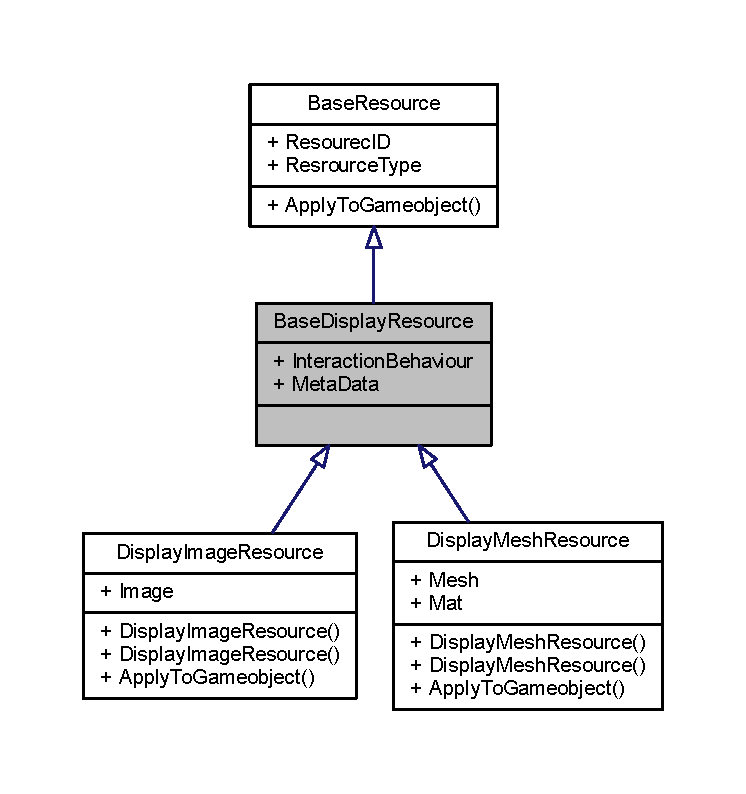
\includegraphics[width=350pt]{class_base_display_resource__inherit__graph}
\end{center}
\end{figure}


Collaboration diagram for Base\+Display\+Resource\+:
\nopagebreak
\begin{figure}[H]
\begin{center}
\leavevmode
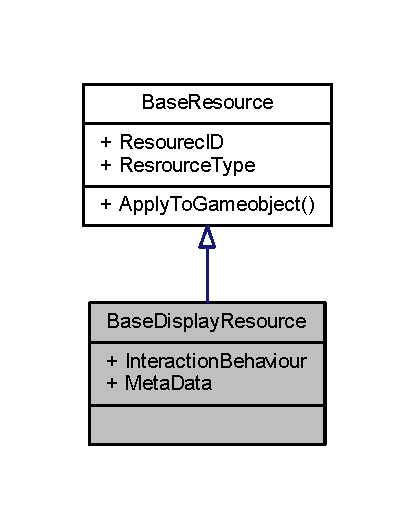
\includegraphics[width=199pt]{class_base_display_resource__coll__graph}
\end{center}
\end{figure}
\subsection*{Public Attributes}
\begin{DoxyCompactItemize}
\item 
string \mbox{\hyperlink{class_base_display_resource_a076a3844786354934f897ff2e9b24a18}{Interaction\+Behaviour}} = \char`\"{}\char`\"{}
\begin{DoxyCompactList}\small\item\em The interaction behaviour the display wants to provide \end{DoxyCompactList}\end{DoxyCompactItemize}
\subsection*{Properties}
\begin{DoxyCompactItemize}
\item 
\mbox{\hyperlink{class_meta_data}{Meta\+Data}} \mbox{\hyperlink{class_base_display_resource_a0a9f0a877d169dd6c5c07c66ae563618}{Meta\+Data}}\hspace{0.3cm}{\ttfamily  \mbox{[}get, protected set\mbox{]}}
\begin{DoxyCompactList}\small\item\em The Metadata associated with this display resource \end{DoxyCompactList}\end{DoxyCompactItemize}
\subsection*{Additional Inherited Members}


\subsection{Detailed Description}
base class for resource 



\subsection{Member Data Documentation}
\mbox{\Hypertarget{class_base_display_resource_a076a3844786354934f897ff2e9b24a18}\label{class_base_display_resource_a076a3844786354934f897ff2e9b24a18}} 
\index{Base\+Display\+Resource@{Base\+Display\+Resource}!Interaction\+Behaviour@{Interaction\+Behaviour}}
\index{Interaction\+Behaviour@{Interaction\+Behaviour}!Base\+Display\+Resource@{Base\+Display\+Resource}}
\subsubsection{\texorpdfstring{Interaction\+Behaviour}{InteractionBehaviour}}
{\footnotesize\ttfamily string Base\+Display\+Resource.\+Interaction\+Behaviour = \char`\"{}\char`\"{}}



The interaction behaviour the display wants to provide 



\subsection{Property Documentation}
\mbox{\Hypertarget{class_base_display_resource_a0a9f0a877d169dd6c5c07c66ae563618}\label{class_base_display_resource_a0a9f0a877d169dd6c5c07c66ae563618}} 
\index{Base\+Display\+Resource@{Base\+Display\+Resource}!Meta\+Data@{Meta\+Data}}
\index{Meta\+Data@{Meta\+Data}!Base\+Display\+Resource@{Base\+Display\+Resource}}
\subsubsection{\texorpdfstring{Meta\+Data}{MetaData}}
{\footnotesize\ttfamily \mbox{\hyperlink{class_meta_data}{Meta\+Data}} Base\+Display\+Resource.\+Meta\+Data\hspace{0.3cm}{\ttfamily [get]}, {\ttfamily [protected set]}}



The Metadata associated with this display resource 



The documentation for this class was generated from the following file\+:\begin{DoxyCompactItemize}
\item 
C\+:/\+Unity\+Projects/\+Virt\+Muse/\+Room\+Gen\+Prototype/\+Assets/\+Scripts/\+Resources/\mbox{\hyperlink{_resource_8cs}{Resource.\+cs}}\end{DoxyCompactItemize}

\hypertarget{class_base_door}{}\section{Base\+Door Class Reference}
\label{class_base_door}\index{Base\+Door@{Base\+Door}}


Inheritance diagram for Base\+Door\+:\nopagebreak
\begin{figure}[H]
\begin{center}
\leavevmode
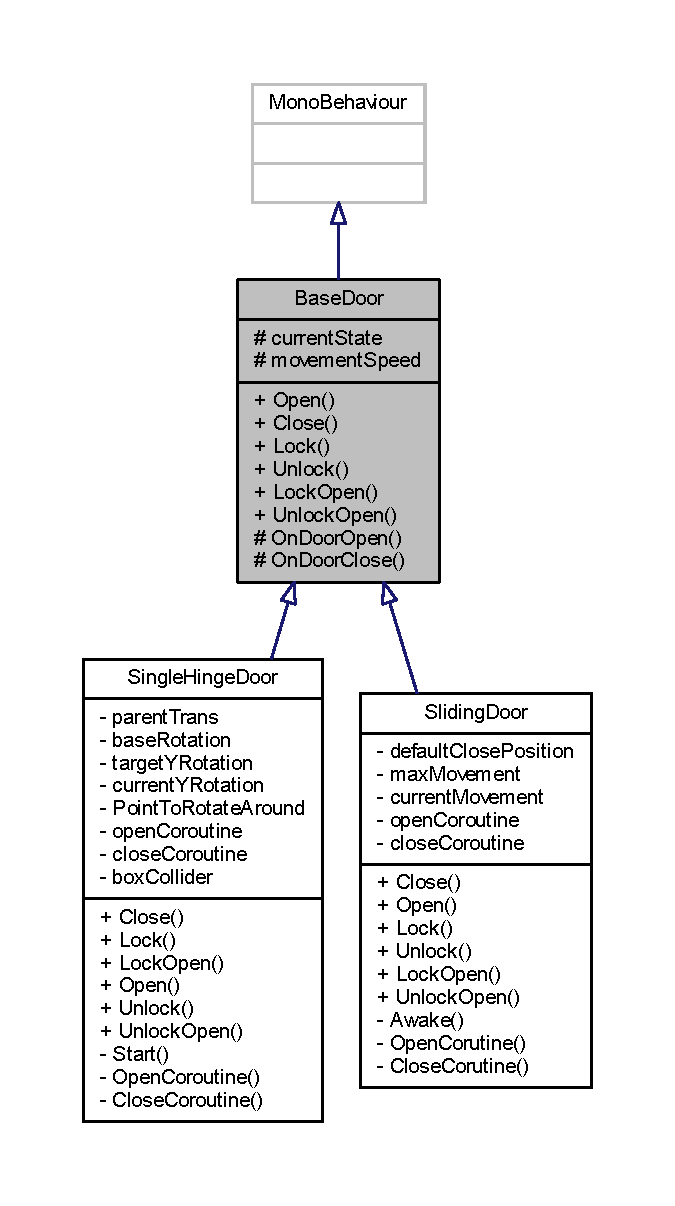
\includegraphics[height=550pt]{class_base_door__inherit__graph}
\end{center}
\end{figure}


Collaboration diagram for Base\+Door\+:\nopagebreak
\begin{figure}[H]
\begin{center}
\leavevmode
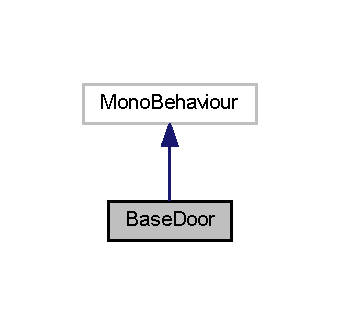
\includegraphics[width=177pt]{class_base_door__coll__graph}
\end{center}
\end{figure}
\subsection*{Public Types}
\begin{DoxyCompactItemize}
\item 
enum \mbox{\hyperlink{class_base_door_a22e038571daf23b362eb8aaedc78cb43}{Door\+State}} \{ \newline
\mbox{\hyperlink{class_base_door_a22e038571daf23b362eb8aaedc78cb43ac3bf447eabe632720a3aa1a7ce401274}{Door\+State.\+Open}}, 
\mbox{\hyperlink{class_base_door_a22e038571daf23b362eb8aaedc78cb43a9bd99a0beea48f10663fc4a7d7a33140}{Door\+State.\+Opening}}, 
\mbox{\hyperlink{class_base_door_a22e038571daf23b362eb8aaedc78cb43a03f4a47830f97377a35321051685071e}{Door\+State.\+Closed}}, 
\mbox{\hyperlink{class_base_door_a22e038571daf23b362eb8aaedc78cb43a5c8de6f894682fdb1786037b2040a26e}{Door\+State.\+Closing}}, 
\newline
\mbox{\hyperlink{class_base_door_a22e038571daf23b362eb8aaedc78cb43a79e87b5071e987722119d21ac38e9b0b}{Door\+State.\+Locked\+Close}}, 
\mbox{\hyperlink{class_base_door_a22e038571daf23b362eb8aaedc78cb43ac3c271ab63e95ff3d1b0e1eac01c9e90}{Door\+State.\+Locked\+Open}}
 \}
\end{DoxyCompactItemize}
\subsection*{Public Member Functions}
\begin{DoxyCompactItemize}
\item 
abstract void \mbox{\hyperlink{class_base_door_a418df6f73cc5c56b6989c0512a6a909b}{Open}} ()
\begin{DoxyCompactList}\small\item\em function called to open the door \end{DoxyCompactList}\item 
abstract void \mbox{\hyperlink{class_base_door_a94151e5cbf90bd3d2b55f339b87916c7}{Close}} ()
\begin{DoxyCompactList}\small\item\em function called to close door \end{DoxyCompactList}\item 
abstract void \mbox{\hyperlink{class_base_door_a2b616c52626299f25ac25f7deab44dc4}{Lock}} (string key)
\begin{DoxyCompactList}\small\item\em function called to lock a door closed \end{DoxyCompactList}\item 
abstract void \mbox{\hyperlink{class_base_door_a1fe85317a4742aec4d03deb7c0d52fd2}{Unlock}} (string key)
\begin{DoxyCompactList}\small\item\em function to unlock a door if it is locked \end{DoxyCompactList}\item 
abstract void \mbox{\hyperlink{class_base_door_a9a851525c3b6e878bec459992ac75408}{Lock\+Open}} ()
\begin{DoxyCompactList}\small\item\em function to lock a door open and stop it from closing \end{DoxyCompactList}\item 
abstract void \mbox{\hyperlink{class_base_door_aae09177b7a5578ede6d44f758551684e}{Unlock\+Open}} ()
\begin{DoxyCompactList}\small\item\em function to unlock a door from it\textquotesingle{}s forced open state \end{DoxyCompactList}\end{DoxyCompactItemize}
\subsection*{Protected Member Functions}
\begin{DoxyCompactItemize}
\item 
void \mbox{\hyperlink{class_base_door_af53bd804dcee24b1f2019c2d2e8e03c6}{On\+Door\+Open}} ()
\begin{DoxyCompactList}\small\item\em wrapper class to invoke event from sub classes \end{DoxyCompactList}\item 
void \mbox{\hyperlink{class_base_door_a3ce14aa6aca622f9d18e7054e76ec8d2}{On\+Door\+Close}} ()
\begin{DoxyCompactList}\small\item\em wrapper function to invoke event from sub classes \end{DoxyCompactList}\end{DoxyCompactItemize}
\subsection*{Protected Attributes}
\begin{DoxyCompactItemize}
\item 
\mbox{\hyperlink{class_base_door_a22e038571daf23b362eb8aaedc78cb43}{Door\+State}} \mbox{\hyperlink{class_base_door_a79de3a0eaae4ea2749f384224dce6692}{current\+State}}
\begin{DoxyCompactList}\small\item\em the current state of the door \end{DoxyCompactList}\item 
float \mbox{\hyperlink{class_base_door_aace8dcf06aaae9d78ebd0d55931ab3e3}{movement\+Speed}}
\begin{DoxyCompactList}\small\item\em the movement speed of the door when opening and closing \end{DoxyCompactList}\end{DoxyCompactItemize}
\subsection*{Events}
\begin{DoxyCompactItemize}
\item 
Action$<$ \mbox{\hyperlink{class_base_door}{Base\+Door}} $>$ \mbox{\hyperlink{class_base_door_a88b84b3eafa96f6a3290b0aa5b55d9c0}{On\+Open}}
\begin{DoxyCompactList}\small\item\em event invoked when the door reaches open state \end{DoxyCompactList}\item 
Action$<$ \mbox{\hyperlink{class_base_door}{Base\+Door}} $>$ \mbox{\hyperlink{class_base_door_a382fd7054c500c9075ef67792f39eab5}{On\+Close}}
\begin{DoxyCompactList}\small\item\em event invoked when the door reaches closed state \end{DoxyCompactList}\end{DoxyCompactItemize}


\subsection{Member Enumeration Documentation}
\mbox{\Hypertarget{class_base_door_a22e038571daf23b362eb8aaedc78cb43}\label{class_base_door_a22e038571daf23b362eb8aaedc78cb43}} 
\index{Base\+Door@{Base\+Door}!Door\+State@{Door\+State}}
\index{Door\+State@{Door\+State}!Base\+Door@{Base\+Door}}
\subsubsection{\texorpdfstring{Door\+State}{DoorState}}
{\footnotesize\ttfamily enum \mbox{\hyperlink{class_base_door_a22e038571daf23b362eb8aaedc78cb43}{Base\+Door.\+Door\+State}}\hspace{0.3cm}{\ttfamily [strong]}}

\begin{DoxyEnumFields}{Enumerator}
\raisebox{\heightof{T}}[0pt][0pt]{\index{Open@{Open}!Base\+Door@{Base\+Door}}\index{Base\+Door@{Base\+Door}!Open@{Open}}}\mbox{\Hypertarget{class_base_door_a22e038571daf23b362eb8aaedc78cb43ac3bf447eabe632720a3aa1a7ce401274}\label{class_base_door_a22e038571daf23b362eb8aaedc78cb43ac3bf447eabe632720a3aa1a7ce401274}} 
Open&\\
\hline

\raisebox{\heightof{T}}[0pt][0pt]{\index{Opening@{Opening}!Base\+Door@{Base\+Door}}\index{Base\+Door@{Base\+Door}!Opening@{Opening}}}\mbox{\Hypertarget{class_base_door_a22e038571daf23b362eb8aaedc78cb43a9bd99a0beea48f10663fc4a7d7a33140}\label{class_base_door_a22e038571daf23b362eb8aaedc78cb43a9bd99a0beea48f10663fc4a7d7a33140}} 
Opening&\\
\hline

\raisebox{\heightof{T}}[0pt][0pt]{\index{Closed@{Closed}!Base\+Door@{Base\+Door}}\index{Base\+Door@{Base\+Door}!Closed@{Closed}}}\mbox{\Hypertarget{class_base_door_a22e038571daf23b362eb8aaedc78cb43a03f4a47830f97377a35321051685071e}\label{class_base_door_a22e038571daf23b362eb8aaedc78cb43a03f4a47830f97377a35321051685071e}} 
Closed&\\
\hline

\raisebox{\heightof{T}}[0pt][0pt]{\index{Closing@{Closing}!Base\+Door@{Base\+Door}}\index{Base\+Door@{Base\+Door}!Closing@{Closing}}}\mbox{\Hypertarget{class_base_door_a22e038571daf23b362eb8aaedc78cb43a5c8de6f894682fdb1786037b2040a26e}\label{class_base_door_a22e038571daf23b362eb8aaedc78cb43a5c8de6f894682fdb1786037b2040a26e}} 
Closing&\\
\hline

\raisebox{\heightof{T}}[0pt][0pt]{\index{Locked\+Close@{Locked\+Close}!Base\+Door@{Base\+Door}}\index{Base\+Door@{Base\+Door}!Locked\+Close@{Locked\+Close}}}\mbox{\Hypertarget{class_base_door_a22e038571daf23b362eb8aaedc78cb43a79e87b5071e987722119d21ac38e9b0b}\label{class_base_door_a22e038571daf23b362eb8aaedc78cb43a79e87b5071e987722119d21ac38e9b0b}} 
Locked\+Close&\\
\hline

\raisebox{\heightof{T}}[0pt][0pt]{\index{Locked\+Open@{Locked\+Open}!Base\+Door@{Base\+Door}}\index{Base\+Door@{Base\+Door}!Locked\+Open@{Locked\+Open}}}\mbox{\Hypertarget{class_base_door_a22e038571daf23b362eb8aaedc78cb43ac3c271ab63e95ff3d1b0e1eac01c9e90}\label{class_base_door_a22e038571daf23b362eb8aaedc78cb43ac3c271ab63e95ff3d1b0e1eac01c9e90}} 
Locked\+Open&\\
\hline

\end{DoxyEnumFields}


\subsection{Member Function Documentation}
\mbox{\Hypertarget{class_base_door_a94151e5cbf90bd3d2b55f339b87916c7}\label{class_base_door_a94151e5cbf90bd3d2b55f339b87916c7}} 
\index{Base\+Door@{Base\+Door}!Close@{Close}}
\index{Close@{Close}!Base\+Door@{Base\+Door}}
\subsubsection{\texorpdfstring{Close()}{Close()}}
{\footnotesize\ttfamily abstract void Base\+Door.\+Close (\begin{DoxyParamCaption}{ }\end{DoxyParamCaption})\hspace{0.3cm}{\ttfamily [pure virtual]}}



function called to close door 



Implemented in \mbox{\hyperlink{class_single_hinge_door_a19848e36fb259f92594916d1af76d3b4}{Single\+Hinge\+Door}}, and \mbox{\hyperlink{class_sliding_door_a22d2e8580503b045da48510214599746}{Sliding\+Door}}.

Here is the caller graph for this function\+:\nopagebreak
\begin{figure}[H]
\begin{center}
\leavevmode
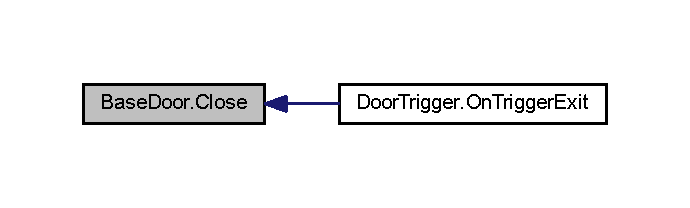
\includegraphics[width=331pt]{class_base_door_a94151e5cbf90bd3d2b55f339b87916c7_icgraph}
\end{center}
\end{figure}
\mbox{\Hypertarget{class_base_door_a2b616c52626299f25ac25f7deab44dc4}\label{class_base_door_a2b616c52626299f25ac25f7deab44dc4}} 
\index{Base\+Door@{Base\+Door}!Lock@{Lock}}
\index{Lock@{Lock}!Base\+Door@{Base\+Door}}
\subsubsection{\texorpdfstring{Lock()}{Lock()}}
{\footnotesize\ttfamily abstract void Base\+Door.\+Lock (\begin{DoxyParamCaption}\item[{string}]{key }\end{DoxyParamCaption})\hspace{0.3cm}{\ttfamily [pure virtual]}}



function called to lock a door closed 


\begin{DoxyParams}{Parameters}
{\em key} & the key needed to lock the door\\
\hline
\end{DoxyParams}


Implemented in \mbox{\hyperlink{class_single_hinge_door_a329ff33388675ec531996bdb33dd0c70}{Single\+Hinge\+Door}}, and \mbox{\hyperlink{class_sliding_door_a2b21b6ea3181ac95520e0490c900d1a6}{Sliding\+Door}}.

Here is the caller graph for this function\+:
\nopagebreak
\begin{figure}[H]
\begin{center}
\leavevmode
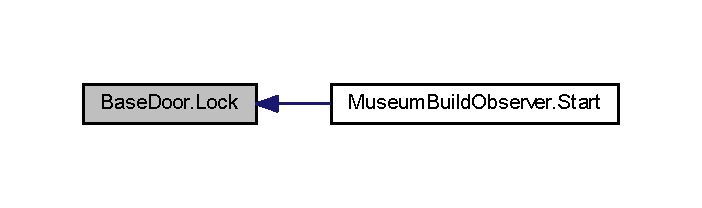
\includegraphics[width=337pt]{class_base_door_a2b616c52626299f25ac25f7deab44dc4_icgraph}
\end{center}
\end{figure}
\mbox{\Hypertarget{class_base_door_a9a851525c3b6e878bec459992ac75408}\label{class_base_door_a9a851525c3b6e878bec459992ac75408}} 
\index{Base\+Door@{Base\+Door}!Lock\+Open@{Lock\+Open}}
\index{Lock\+Open@{Lock\+Open}!Base\+Door@{Base\+Door}}
\subsubsection{\texorpdfstring{Lock\+Open()}{LockOpen()}}
{\footnotesize\ttfamily abstract void Base\+Door.\+Lock\+Open (\begin{DoxyParamCaption}{ }\end{DoxyParamCaption})\hspace{0.3cm}{\ttfamily [pure virtual]}}



function to lock a door open and stop it from closing 



Implemented in \mbox{\hyperlink{class_sliding_door_aca96469919dc50b5b3cc77cd6f4fc7d2}{Sliding\+Door}}, and \mbox{\hyperlink{class_single_hinge_door_aea7072ec0a9ea4fc80f24dc400681478}{Single\+Hinge\+Door}}.

Here is the caller graph for this function\+:
\nopagebreak
\begin{figure}[H]
\begin{center}
\leavevmode
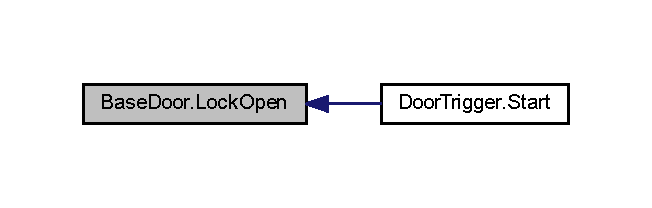
\includegraphics[width=313pt]{class_base_door_a9a851525c3b6e878bec459992ac75408_icgraph}
\end{center}
\end{figure}
\mbox{\Hypertarget{class_base_door_a3ce14aa6aca622f9d18e7054e76ec8d2}\label{class_base_door_a3ce14aa6aca622f9d18e7054e76ec8d2}} 
\index{Base\+Door@{Base\+Door}!On\+Door\+Close@{On\+Door\+Close}}
\index{On\+Door\+Close@{On\+Door\+Close}!Base\+Door@{Base\+Door}}
\subsubsection{\texorpdfstring{On\+Door\+Close()}{OnDoorClose()}}
{\footnotesize\ttfamily void Base\+Door.\+On\+Door\+Close (\begin{DoxyParamCaption}{ }\end{DoxyParamCaption})\hspace{0.3cm}{\ttfamily [protected]}}



wrapper function to invoke event from sub classes 

Here is the caller graph for this function\+:
\nopagebreak
\begin{figure}[H]
\begin{center}
\leavevmode
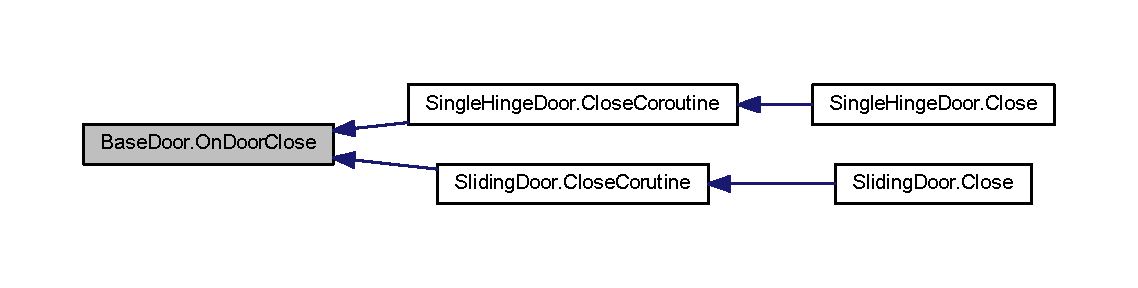
\includegraphics[width=350pt]{class_base_door_a3ce14aa6aca622f9d18e7054e76ec8d2_icgraph}
\end{center}
\end{figure}
\mbox{\Hypertarget{class_base_door_af53bd804dcee24b1f2019c2d2e8e03c6}\label{class_base_door_af53bd804dcee24b1f2019c2d2e8e03c6}} 
\index{Base\+Door@{Base\+Door}!On\+Door\+Open@{On\+Door\+Open}}
\index{On\+Door\+Open@{On\+Door\+Open}!Base\+Door@{Base\+Door}}
\subsubsection{\texorpdfstring{On\+Door\+Open()}{OnDoorOpen()}}
{\footnotesize\ttfamily void Base\+Door.\+On\+Door\+Open (\begin{DoxyParamCaption}{ }\end{DoxyParamCaption})\hspace{0.3cm}{\ttfamily [protected]}}



wrapper class to invoke event from sub classes 

Here is the caller graph for this function\+:
\nopagebreak
\begin{figure}[H]
\begin{center}
\leavevmode
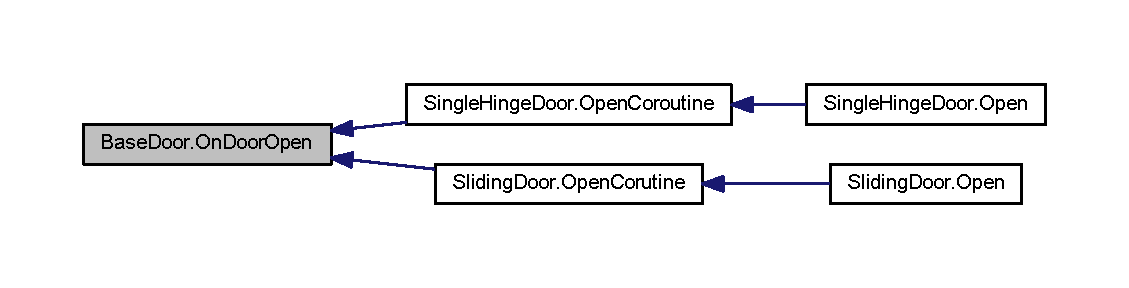
\includegraphics[width=350pt]{class_base_door_af53bd804dcee24b1f2019c2d2e8e03c6_icgraph}
\end{center}
\end{figure}
\mbox{\Hypertarget{class_base_door_a418df6f73cc5c56b6989c0512a6a909b}\label{class_base_door_a418df6f73cc5c56b6989c0512a6a909b}} 
\index{Base\+Door@{Base\+Door}!Open@{Open}}
\index{Open@{Open}!Base\+Door@{Base\+Door}}
\subsubsection{\texorpdfstring{Open()}{Open()}}
{\footnotesize\ttfamily abstract void Base\+Door.\+Open (\begin{DoxyParamCaption}{ }\end{DoxyParamCaption})\hspace{0.3cm}{\ttfamily [pure virtual]}}



function called to open the door 



Implemented in \mbox{\hyperlink{class_single_hinge_door_ad48e670701a9e9d35f97de3b8ff36208}{Single\+Hinge\+Door}}, and \mbox{\hyperlink{class_sliding_door_aaf090e96cc143eb5ed3eaf875045efc9}{Sliding\+Door}}.

Here is the caller graph for this function\+:
\nopagebreak
\begin{figure}[H]
\begin{center}
\leavevmode
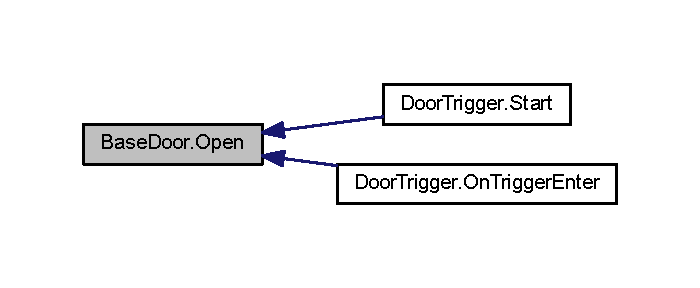
\includegraphics[width=336pt]{class_base_door_a418df6f73cc5c56b6989c0512a6a909b_icgraph}
\end{center}
\end{figure}
\mbox{\Hypertarget{class_base_door_a1fe85317a4742aec4d03deb7c0d52fd2}\label{class_base_door_a1fe85317a4742aec4d03deb7c0d52fd2}} 
\index{Base\+Door@{Base\+Door}!Unlock@{Unlock}}
\index{Unlock@{Unlock}!Base\+Door@{Base\+Door}}
\subsubsection{\texorpdfstring{Unlock()}{Unlock()}}
{\footnotesize\ttfamily abstract void Base\+Door.\+Unlock (\begin{DoxyParamCaption}\item[{string}]{key }\end{DoxyParamCaption})\hspace{0.3cm}{\ttfamily [pure virtual]}}



function to unlock a door if it is locked 


\begin{DoxyParams}{Parameters}
{\em key} & the key needed to unlock it\\
\hline
\end{DoxyParams}


Implemented in \mbox{\hyperlink{class_single_hinge_door_a130d674b08d4b9e8028b08ef2084ab77}{Single\+Hinge\+Door}}, and \mbox{\hyperlink{class_sliding_door_a259817872880d475d54ba9721a6db5cc}{Sliding\+Door}}.

Here is the caller graph for this function\+:
\nopagebreak
\begin{figure}[H]
\begin{center}
\leavevmode
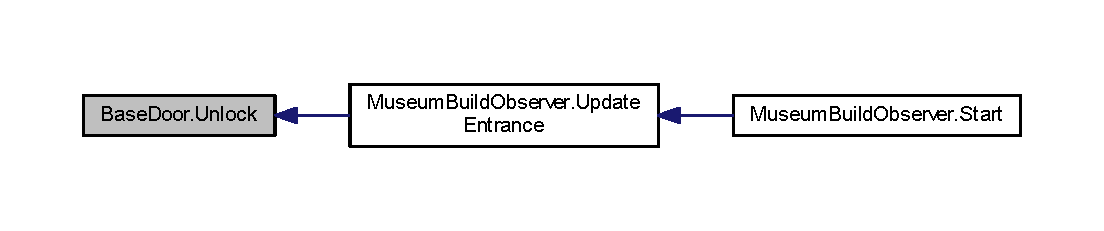
\includegraphics[width=350pt]{class_base_door_a1fe85317a4742aec4d03deb7c0d52fd2_icgraph}
\end{center}
\end{figure}
\mbox{\Hypertarget{class_base_door_aae09177b7a5578ede6d44f758551684e}\label{class_base_door_aae09177b7a5578ede6d44f758551684e}} 
\index{Base\+Door@{Base\+Door}!Unlock\+Open@{Unlock\+Open}}
\index{Unlock\+Open@{Unlock\+Open}!Base\+Door@{Base\+Door}}
\subsubsection{\texorpdfstring{Unlock\+Open()}{UnlockOpen()}}
{\footnotesize\ttfamily abstract void Base\+Door.\+Unlock\+Open (\begin{DoxyParamCaption}{ }\end{DoxyParamCaption})\hspace{0.3cm}{\ttfamily [pure virtual]}}



function to unlock a door from it\textquotesingle{}s forced open state 



Implemented in \mbox{\hyperlink{class_single_hinge_door_a5e5785f02f35b8b109d4c50d3f912013}{Single\+Hinge\+Door}}, and \mbox{\hyperlink{class_sliding_door_af3b93ba6356b95277be1913224ad1415}{Sliding\+Door}}.



\subsection{Member Data Documentation}
\mbox{\Hypertarget{class_base_door_a79de3a0eaae4ea2749f384224dce6692}\label{class_base_door_a79de3a0eaae4ea2749f384224dce6692}} 
\index{Base\+Door@{Base\+Door}!current\+State@{current\+State}}
\index{current\+State@{current\+State}!Base\+Door@{Base\+Door}}
\subsubsection{\texorpdfstring{current\+State}{currentState}}
{\footnotesize\ttfamily \mbox{\hyperlink{class_base_door_a22e038571daf23b362eb8aaedc78cb43}{Door\+State}} Base\+Door.\+current\+State\hspace{0.3cm}{\ttfamily [protected]}}



the current state of the door 

\mbox{\Hypertarget{class_base_door_aace8dcf06aaae9d78ebd0d55931ab3e3}\label{class_base_door_aace8dcf06aaae9d78ebd0d55931ab3e3}} 
\index{Base\+Door@{Base\+Door}!movement\+Speed@{movement\+Speed}}
\index{movement\+Speed@{movement\+Speed}!Base\+Door@{Base\+Door}}
\subsubsection{\texorpdfstring{movement\+Speed}{movementSpeed}}
{\footnotesize\ttfamily float Base\+Door.\+movement\+Speed\hspace{0.3cm}{\ttfamily [protected]}}



the movement speed of the door when opening and closing 



\subsection{Event Documentation}
\mbox{\Hypertarget{class_base_door_a382fd7054c500c9075ef67792f39eab5}\label{class_base_door_a382fd7054c500c9075ef67792f39eab5}} 
\index{Base\+Door@{Base\+Door}!On\+Close@{On\+Close}}
\index{On\+Close@{On\+Close}!Base\+Door@{Base\+Door}}
\subsubsection{\texorpdfstring{On\+Close}{OnClose}}
{\footnotesize\ttfamily Action$<$\mbox{\hyperlink{class_base_door}{Base\+Door}}$>$ Base\+Door.\+On\+Close}



event invoked when the door reaches closed state 

\mbox{\Hypertarget{class_base_door_a88b84b3eafa96f6a3290b0aa5b55d9c0}\label{class_base_door_a88b84b3eafa96f6a3290b0aa5b55d9c0}} 
\index{Base\+Door@{Base\+Door}!On\+Open@{On\+Open}}
\index{On\+Open@{On\+Open}!Base\+Door@{Base\+Door}}
\subsubsection{\texorpdfstring{On\+Open}{OnOpen}}
{\footnotesize\ttfamily Action$<$\mbox{\hyperlink{class_base_door}{Base\+Door}}$>$ Base\+Door.\+On\+Open}



event invoked when the door reaches open state 



The documentation for this class was generated from the following file\+:\begin{DoxyCompactItemize}
\item 
C\+:/\+Unity\+Projects/\+Virt\+Muse/\+Room\+Gen\+Prototype/\+Assets/\+Scripts/\+Door/\mbox{\hyperlink{_base_door_8cs}{Base\+Door.\+cs}}\end{DoxyCompactItemize}

\hypertarget{class_base_resource}{}\section{Base\+Resource Class Reference}
\label{class_base_resource}\index{Base\+Resource@{Base\+Resource}}


base class for any resource be it display resource or other  




Inheritance diagram for Base\+Resource\+:
\nopagebreak
\begin{figure}[H]
\begin{center}
\leavevmode
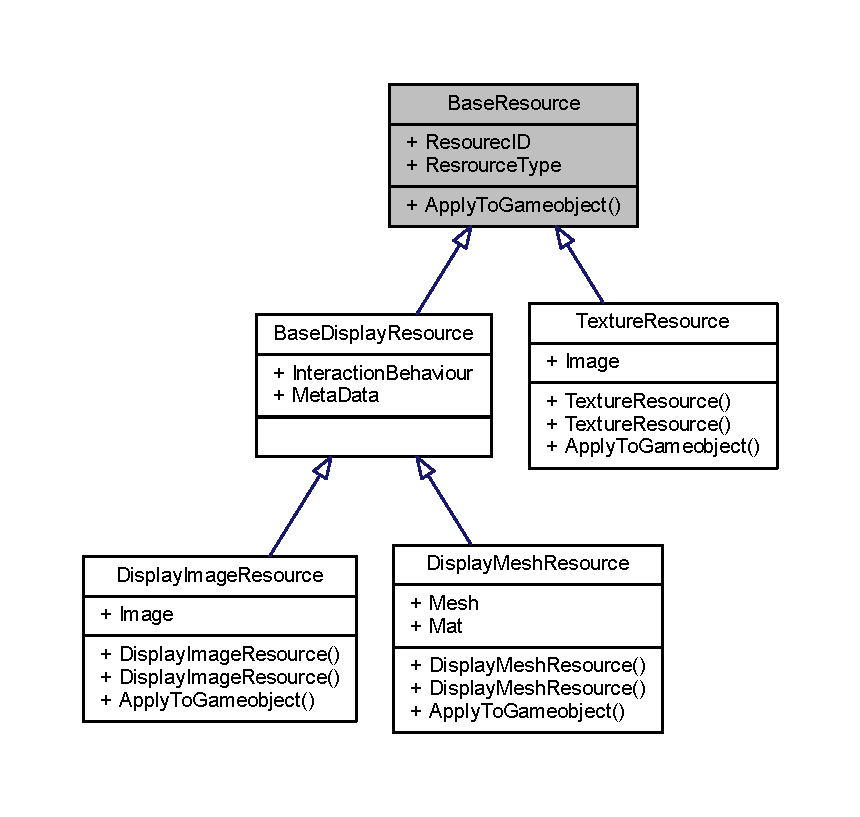
\includegraphics[width=328pt]{class_base_resource__inherit__graph}
\end{center}
\end{figure}
\subsection*{Public Member Functions}
\begin{DoxyCompactItemize}
\item 
abstract void \mbox{\hyperlink{class_base_resource_a2d832c8042114da9e3f6240651d59703}{Apply\+To\+Gameobject}} (Game\+Object obj)
\begin{DoxyCompactList}\small\item\em function that applies a resource to a gamobject \end{DoxyCompactList}\end{DoxyCompactItemize}
\subsection*{Properties}
\begin{DoxyCompactItemize}
\item 
int \mbox{\hyperlink{class_base_resource_adbdcd8935067e622c993b912a475c21b}{Resourec\+ID}}\hspace{0.3cm}{\ttfamily  \mbox{[}get, set\mbox{]}}
\begin{DoxyCompactList}\small\item\em The resource ID \end{DoxyCompactList}\item 
\mbox{\hyperlink{namespace_virt_muse_web_1_1_models_ab185d30c831a1ac813a53670c29d6397}{Resource\+Type}} \mbox{\hyperlink{class_base_resource_a6c40931e66a2e4fd8061f069eb0c0ba8}{Resrource\+Type}}\hspace{0.3cm}{\ttfamily  \mbox{[}get, set\mbox{]}}
\begin{DoxyCompactList}\small\item\em The type of resource currently\+: Image Mesh \mbox{\hyperlink{class_room_style}{Room\+Style}} \end{DoxyCompactList}\end{DoxyCompactItemize}


\subsection{Detailed Description}
base class for any resource be it display resource or other 



\subsection{Member Function Documentation}
\mbox{\Hypertarget{class_base_resource_a2d832c8042114da9e3f6240651d59703}\label{class_base_resource_a2d832c8042114da9e3f6240651d59703}} 
\index{Base\+Resource@{Base\+Resource}!Apply\+To\+Gameobject@{Apply\+To\+Gameobject}}
\index{Apply\+To\+Gameobject@{Apply\+To\+Gameobject}!Base\+Resource@{Base\+Resource}}
\subsubsection{\texorpdfstring{Apply\+To\+Gameobject()}{ApplyToGameobject()}}
{\footnotesize\ttfamily abstract void Base\+Resource.\+Apply\+To\+Gameobject (\begin{DoxyParamCaption}\item[{Game\+Object}]{obj }\end{DoxyParamCaption})\hspace{0.3cm}{\ttfamily [pure virtual]}}



function that applies a resource to a gamobject 


\begin{DoxyParams}{Parameters}
{\em obj} & the object the resource is applied to\\
\hline
\end{DoxyParams}


Implemented in \mbox{\hyperlink{class_display_image_resource_a26992a5ecb6c449d85539cc5d07112e2}{Display\+Image\+Resource}}, and \mbox{\hyperlink{class_display_mesh_resource_a62672f28a402bebeed1cb79fcca81828}{Display\+Mesh\+Resource}}.

Here is the caller graph for this function\+:
\nopagebreak
\begin{figure}[H]
\begin{center}
\leavevmode
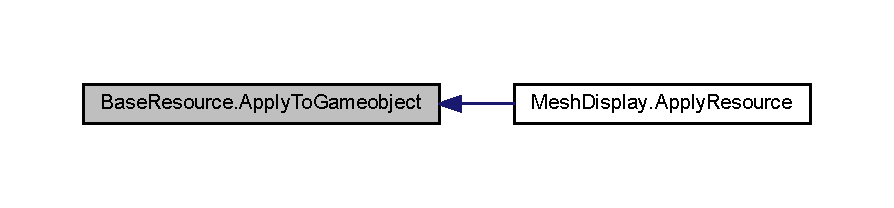
\includegraphics[width=350pt]{class_base_resource_a2d832c8042114da9e3f6240651d59703_icgraph}
\end{center}
\end{figure}


\subsection{Property Documentation}
\mbox{\Hypertarget{class_base_resource_adbdcd8935067e622c993b912a475c21b}\label{class_base_resource_adbdcd8935067e622c993b912a475c21b}} 
\index{Base\+Resource@{Base\+Resource}!Resourec\+ID@{Resourec\+ID}}
\index{Resourec\+ID@{Resourec\+ID}!Base\+Resource@{Base\+Resource}}
\subsubsection{\texorpdfstring{Resourec\+ID}{ResourecID}}
{\footnotesize\ttfamily int Base\+Resource.\+Resourec\+ID\hspace{0.3cm}{\ttfamily [get]}, {\ttfamily [set]}}



The resource ID 

\mbox{\Hypertarget{class_base_resource_a6c40931e66a2e4fd8061f069eb0c0ba8}\label{class_base_resource_a6c40931e66a2e4fd8061f069eb0c0ba8}} 
\index{Base\+Resource@{Base\+Resource}!Resrource\+Type@{Resrource\+Type}}
\index{Resrource\+Type@{Resrource\+Type}!Base\+Resource@{Base\+Resource}}
\subsubsection{\texorpdfstring{Resrource\+Type}{ResrourceType}}
{\footnotesize\ttfamily \mbox{\hyperlink{namespace_virt_muse_web_1_1_models_ab185d30c831a1ac813a53670c29d6397}{Resource\+Type}} Base\+Resource.\+Resrource\+Type\hspace{0.3cm}{\ttfamily [get]}, {\ttfamily [set]}}



The type of resource currently\+: Image Mesh \mbox{\hyperlink{class_room_style}{Room\+Style}} 



The documentation for this class was generated from the following file\+:\begin{DoxyCompactItemize}
\item 
C\+:/\+Unity\+Projects/\+Virt\+Muse/\+Room\+Gen\+Prototype/\+Assets/\+Scripts/\+Resources/\mbox{\hyperlink{_resource_8cs}{Resource.\+cs}}\end{DoxyCompactItemize}

\hypertarget{class_base_room_type_placable_cheker}{}\section{Base\+Room\+Type\+Placable\+Cheker Class Reference}
\label{class_base_room_type_placable_cheker}\index{Base\+Room\+Type\+Placable\+Cheker@{Base\+Room\+Type\+Placable\+Cheker}}


checks for the room types defined by me if they are placable at a certain location in the musem  




Inheritance diagram for Base\+Room\+Type\+Placable\+Cheker\+:
\nopagebreak
\begin{figure}[H]
\begin{center}
\leavevmode
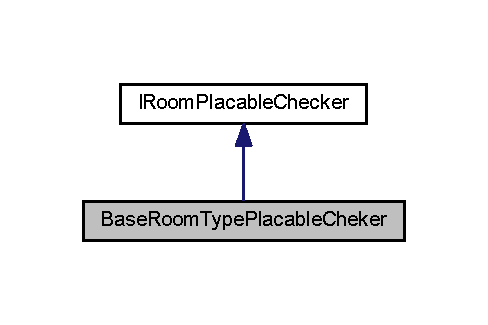
\includegraphics[width=234pt]{class_base_room_type_placable_cheker__inherit__graph}
\end{center}
\end{figure}


Collaboration diagram for Base\+Room\+Type\+Placable\+Cheker\+:
\nopagebreak
\begin{figure}[H]
\begin{center}
\leavevmode
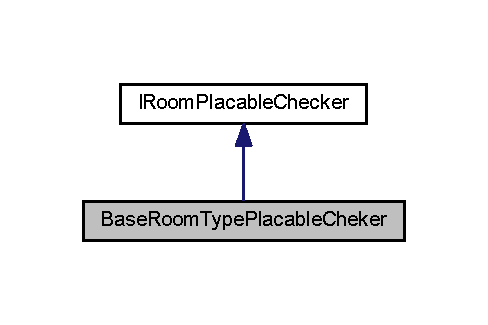
\includegraphics[width=234pt]{class_base_room_type_placable_cheker__coll__graph}
\end{center}
\end{figure}
\subsection*{Public Member Functions}
\begin{DoxyCompactItemize}
\item 
\mbox{\hyperlink{class_base_room_type_placable_cheker_a5d13e7de140af3ba2a4aa12e3724f333}{Base\+Room\+Type\+Placable\+Cheker}} (\mbox{\hyperlink{_room_8cs_ab540f7414f306325d92272bcef1e34e1}{Room\+Type}} type)
\item 
virtual bool \mbox{\hyperlink{class_base_room_type_placable_cheker_a1081710d512b5f2496d390ece6cdbadd}{Check\+If\+Placable}} (Vector2\+Int origin, out List$<$ Vector2\+Int\mbox{[}$\,$\mbox{]}$>$ possible\+Sequences, \mbox{\hyperlink{class_museum}{Museum}} virt\+Muse)
\begin{DoxyCompactList}\small\item\em function that checks if a room is placable at this location in the museum when the musem is gnerated \end{DoxyCompactList}\end{DoxyCompactItemize}
\subsection*{Private Attributes}
\begin{DoxyCompactItemize}
\item 
List$<$ Vector2\+Int\mbox{[}$\,$\mbox{]}$>$ \mbox{\hyperlink{class_base_room_type_placable_cheker_aa1c2ec3105266167905e9be9af7a82be}{step\+Sequences}}
\begin{DoxyCompactList}\small\item\em the type for which this placable checker has been defined \end{DoxyCompactList}\end{DoxyCompactItemize}


\subsection{Detailed Description}
checks for the room types defined by me if they are placable at a certain location in the musem 



\subsection{Constructor \& Destructor Documentation}
\mbox{\Hypertarget{class_base_room_type_placable_cheker_a5d13e7de140af3ba2a4aa12e3724f333}\label{class_base_room_type_placable_cheker_a5d13e7de140af3ba2a4aa12e3724f333}} 
\index{Base\+Room\+Type\+Placable\+Cheker@{Base\+Room\+Type\+Placable\+Cheker}!Base\+Room\+Type\+Placable\+Cheker@{Base\+Room\+Type\+Placable\+Cheker}}
\index{Base\+Room\+Type\+Placable\+Cheker@{Base\+Room\+Type\+Placable\+Cheker}!Base\+Room\+Type\+Placable\+Cheker@{Base\+Room\+Type\+Placable\+Cheker}}
\subsubsection{\texorpdfstring{Base\+Room\+Type\+Placable\+Cheker()}{BaseRoomTypePlacableCheker()}}
{\footnotesize\ttfamily Base\+Room\+Type\+Placable\+Cheker.\+Base\+Room\+Type\+Placable\+Cheker (\begin{DoxyParamCaption}\item[{\mbox{\hyperlink{_room_8cs_ab540f7414f306325d92272bcef1e34e1}{Room\+Type}}}]{type }\end{DoxyParamCaption})}



\subsection{Member Function Documentation}
\mbox{\Hypertarget{class_base_room_type_placable_cheker_a1081710d512b5f2496d390ece6cdbadd}\label{class_base_room_type_placable_cheker_a1081710d512b5f2496d390ece6cdbadd}} 
\index{Base\+Room\+Type\+Placable\+Cheker@{Base\+Room\+Type\+Placable\+Cheker}!Check\+If\+Placable@{Check\+If\+Placable}}
\index{Check\+If\+Placable@{Check\+If\+Placable}!Base\+Room\+Type\+Placable\+Cheker@{Base\+Room\+Type\+Placable\+Cheker}}
\subsubsection{\texorpdfstring{Check\+If\+Placable()}{CheckIfPlacable()}}
{\footnotesize\ttfamily virtual bool Base\+Room\+Type\+Placable\+Cheker.\+Check\+If\+Placable (\begin{DoxyParamCaption}\item[{Vector2\+Int}]{origin,  }\item[{out List$<$ Vector2\+Int\mbox{[}$\,$\mbox{]}$>$}]{possible\+Sequences,  }\item[{\mbox{\hyperlink{class_museum}{Museum}}}]{virt\+Muse }\end{DoxyParamCaption})\hspace{0.3cm}{\ttfamily [virtual]}}



function that checks if a room is placable at this location in the museum when the musem is gnerated 


\begin{DoxyParams}{Parameters}
{\em origin} & the origin position of the room\\
\hline
{\em possible\+Sequences} & out of all the poss directions of steps to build this room type\\
\hline
{\em virt\+Muse} & the virtual museum the room should be placed in\\
\hline
\end{DoxyParams}
\begin{DoxyReturn}{Returns}
ture if room is placable, false if not
\end{DoxyReturn}


Implements \mbox{\hyperlink{interface_i_room_placable_checker_ab4a1591854373fc3b48619dbeb1e2755}{I\+Room\+Placable\+Checker}}.



\subsection{Member Data Documentation}
\mbox{\Hypertarget{class_base_room_type_placable_cheker_aa1c2ec3105266167905e9be9af7a82be}\label{class_base_room_type_placable_cheker_aa1c2ec3105266167905e9be9af7a82be}} 
\index{Base\+Room\+Type\+Placable\+Cheker@{Base\+Room\+Type\+Placable\+Cheker}!step\+Sequences@{step\+Sequences}}
\index{step\+Sequences@{step\+Sequences}!Base\+Room\+Type\+Placable\+Cheker@{Base\+Room\+Type\+Placable\+Cheker}}
\subsubsection{\texorpdfstring{step\+Sequences}{stepSequences}}
{\footnotesize\ttfamily List$<$Vector2\+Int\mbox{[}$\,$\mbox{]}$>$ Base\+Room\+Type\+Placable\+Cheker.\+step\+Sequences\hspace{0.3cm}{\ttfamily [private]}}



the type for which this placable checker has been defined 

the possible steps one can take from the base tile we want to place the room at that can be taken to build this rom shape 

The documentation for this class was generated from the following file\+:\begin{DoxyCompactItemize}
\item 
C\+:/\+Unity\+Projects/\+Virt\+Muse/\+Room\+Gen\+Prototype/\+Assets/\+Scripts/\+Virt\+Museum/\+Room\+\_\+\+Walls/\+Room\+Placable\+Checkers/\mbox{\hyperlink{_base_room_placable_checker_8cs}{Base\+Room\+Placable\+Checker.\+cs}}\end{DoxyCompactItemize}

\hypertarget{class_big_room_wall_validator}{}\section{Big\+Room\+Wall\+Validator Class Reference}
\label{class_big_room_wall_validator}\index{Big\+Room\+Wall\+Validator@{Big\+Room\+Wall\+Validator}}


wall validator for 2x2 rooms  




Inheritance diagram for Big\+Room\+Wall\+Validator\+:
\nopagebreak
\begin{figure}[H]
\begin{center}
\leavevmode
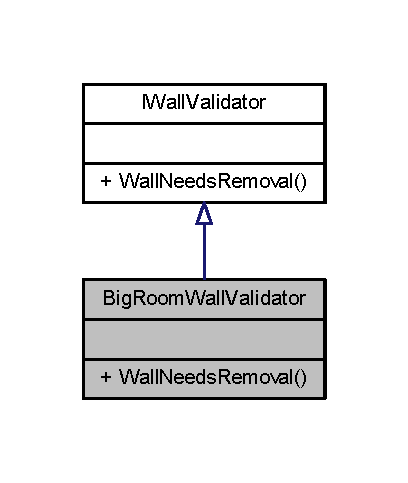
\includegraphics[width=194pt]{class_big_room_wall_validator__inherit__graph}
\end{center}
\end{figure}


Collaboration diagram for Big\+Room\+Wall\+Validator\+:
\nopagebreak
\begin{figure}[H]
\begin{center}
\leavevmode
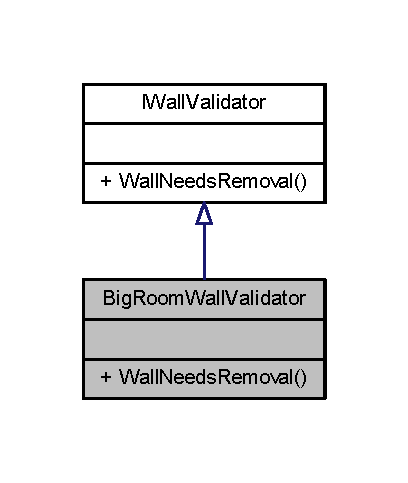
\includegraphics[width=194pt]{class_big_room_wall_validator__coll__graph}
\end{center}
\end{figure}
\subsection*{Public Member Functions}
\begin{DoxyCompactItemize}
\item 
bool \mbox{\hyperlink{class_big_room_wall_validator_abc5968ccc9e70e3d5b8de7ccff2c69bb}{Wall\+Needs\+Removal}} (uint corner\+One\+Count, uint corner\+Two\+Count)
\begin{DoxyCompactList}\small\item\em Checks if this wall needs to be removed for this roomtype by checking how often this corner appearse in all walls for every tile of the room \end{DoxyCompactList}\end{DoxyCompactItemize}


\subsection{Detailed Description}
wall validator for 2x2 rooms 



\subsection{Member Function Documentation}
\mbox{\Hypertarget{class_big_room_wall_validator_abc5968ccc9e70e3d5b8de7ccff2c69bb}\label{class_big_room_wall_validator_abc5968ccc9e70e3d5b8de7ccff2c69bb}} 
\index{Big\+Room\+Wall\+Validator@{Big\+Room\+Wall\+Validator}!Wall\+Needs\+Removal@{Wall\+Needs\+Removal}}
\index{Wall\+Needs\+Removal@{Wall\+Needs\+Removal}!Big\+Room\+Wall\+Validator@{Big\+Room\+Wall\+Validator}}
\subsubsection{\texorpdfstring{Wall\+Needs\+Removal()}{WallNeedsRemoval()}}
{\footnotesize\ttfamily bool Big\+Room\+Wall\+Validator.\+Wall\+Needs\+Removal (\begin{DoxyParamCaption}\item[{uint}]{corner\+One\+Count,  }\item[{uint}]{corner\+Two\+Count }\end{DoxyParamCaption})}



Checks if this wall needs to be removed for this roomtype by checking how often this corner appearse in all walls for every tile of the room 

\begin{DoxyReturn}{Returns}
true if wall is to be kept, false otherwise
\end{DoxyReturn}


Implements \mbox{\hyperlink{interface_i_wall_validator_a1618acf45bf2614985aeb8b240bf7da8}{I\+Wall\+Validator}}.



The documentation for this class was generated from the following file\+:\begin{DoxyCompactItemize}
\item 
C\+:/\+Unity\+Projects/\+Virt\+Muse/\+Room\+Gen\+Prototype/\+Assets/\+Scripts/\+Virt\+Museum/\+Room\+\_\+\+Walls/\+Wall\+Validators/\mbox{\hyperlink{_big_room_wall_validator_8cs}{Big\+Room\+Wall\+Validator.\+cs}}\end{DoxyCompactItemize}

\hypertarget{class_bounding_sphere}{}\section{Bounding\+Sphere Class Reference}
\label{class_bounding_sphere}\index{Bounding\+Sphere@{Bounding\+Sphere}}


Collaboration diagram for Bounding\+Sphere\+:
\nopagebreak
\begin{figure}[H]
\begin{center}
\leavevmode
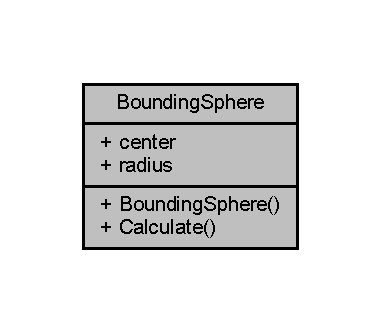
\includegraphics[width=183pt]{class_bounding_sphere__coll__graph}
\end{center}
\end{figure}
\subsection*{Public Member Functions}
\begin{DoxyCompactItemize}
\item 
\mbox{\hyperlink{class_bounding_sphere_ad35e7960a2e532e8f7cbebbca2136ef7}{Bounding\+Sphere}} (Vector3 a\+Center, float a\+Radius)
\end{DoxyCompactItemize}
\subsection*{Static Public Member Functions}
\begin{DoxyCompactItemize}
\item 
static \mbox{\hyperlink{class_bounding_sphere}{Bounding\+Sphere}} \mbox{\hyperlink{class_bounding_sphere_a29c277d13a701089666b94fabf3c87d6}{Calculate}} (I\+Enumerable$<$ Vector3 $>$ a\+Points)
\begin{DoxyCompactList}\small\item\em calculates a bounding sphrere for a given list of vertices \end{DoxyCompactList}\end{DoxyCompactItemize}
\subsection*{Public Attributes}
\begin{DoxyCompactItemize}
\item 
Vector3 \mbox{\hyperlink{class_bounding_sphere_a0996d0f450c5e7fcca8446ebbd8ddc20}{center}}
\begin{DoxyCompactList}\small\item\em center of the bounding sphre \end{DoxyCompactList}\item 
float \mbox{\hyperlink{class_bounding_sphere_ad507cd54bc4021617024c2545fe9379c}{radius}}
\begin{DoxyCompactList}\small\item\em radius of bounding sphere \end{DoxyCompactList}\end{DoxyCompactItemize}


\subsection{Constructor \& Destructor Documentation}
\mbox{\Hypertarget{class_bounding_sphere_ad35e7960a2e532e8f7cbebbca2136ef7}\label{class_bounding_sphere_ad35e7960a2e532e8f7cbebbca2136ef7}} 
\index{Bounding\+Sphere@{Bounding\+Sphere}!Bounding\+Sphere@{Bounding\+Sphere}}
\index{Bounding\+Sphere@{Bounding\+Sphere}!Bounding\+Sphere@{Bounding\+Sphere}}
\subsubsection{\texorpdfstring{Bounding\+Sphere()}{BoundingSphere()}}
{\footnotesize\ttfamily Bounding\+Sphere.\+Bounding\+Sphere (\begin{DoxyParamCaption}\item[{Vector3}]{a\+Center,  }\item[{float}]{a\+Radius }\end{DoxyParamCaption})}

Here is the caller graph for this function\+:
\nopagebreak
\begin{figure}[H]
\begin{center}
\leavevmode
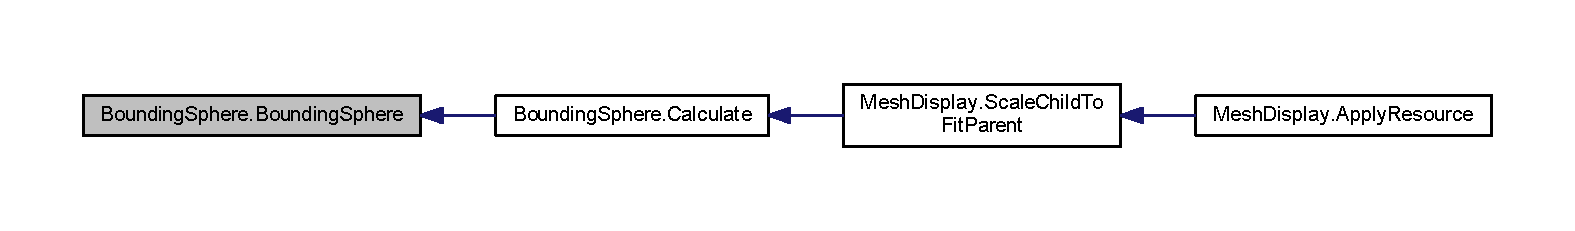
\includegraphics[width=350pt]{class_bounding_sphere_ad35e7960a2e532e8f7cbebbca2136ef7_icgraph}
\end{center}
\end{figure}


\subsection{Member Function Documentation}
\mbox{\Hypertarget{class_bounding_sphere_a29c277d13a701089666b94fabf3c87d6}\label{class_bounding_sphere_a29c277d13a701089666b94fabf3c87d6}} 
\index{Bounding\+Sphere@{Bounding\+Sphere}!Calculate@{Calculate}}
\index{Calculate@{Calculate}!Bounding\+Sphere@{Bounding\+Sphere}}
\subsubsection{\texorpdfstring{Calculate()}{Calculate()}}
{\footnotesize\ttfamily static \mbox{\hyperlink{class_bounding_sphere}{Bounding\+Sphere}} Bounding\+Sphere.\+Calculate (\begin{DoxyParamCaption}\item[{I\+Enumerable$<$ Vector3 $>$}]{a\+Points }\end{DoxyParamCaption})\hspace{0.3cm}{\ttfamily [static]}}



calculates a bounding sphrere for a given list of vertices 


\begin{DoxyParams}{Parameters}
{\em a\+Points} & the list of vertices for whom the bounding sphere should be calculated\\
\hline
\end{DoxyParams}
\begin{DoxyReturn}{Returns}
the bounding sphere
\end{DoxyReturn}
Here is the call graph for this function\+:
\nopagebreak
\begin{figure}[H]
\begin{center}
\leavevmode
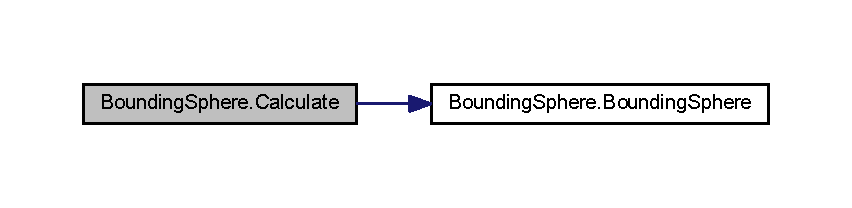
\includegraphics[width=350pt]{class_bounding_sphere_a29c277d13a701089666b94fabf3c87d6_cgraph}
\end{center}
\end{figure}
Here is the caller graph for this function\+:
\nopagebreak
\begin{figure}[H]
\begin{center}
\leavevmode
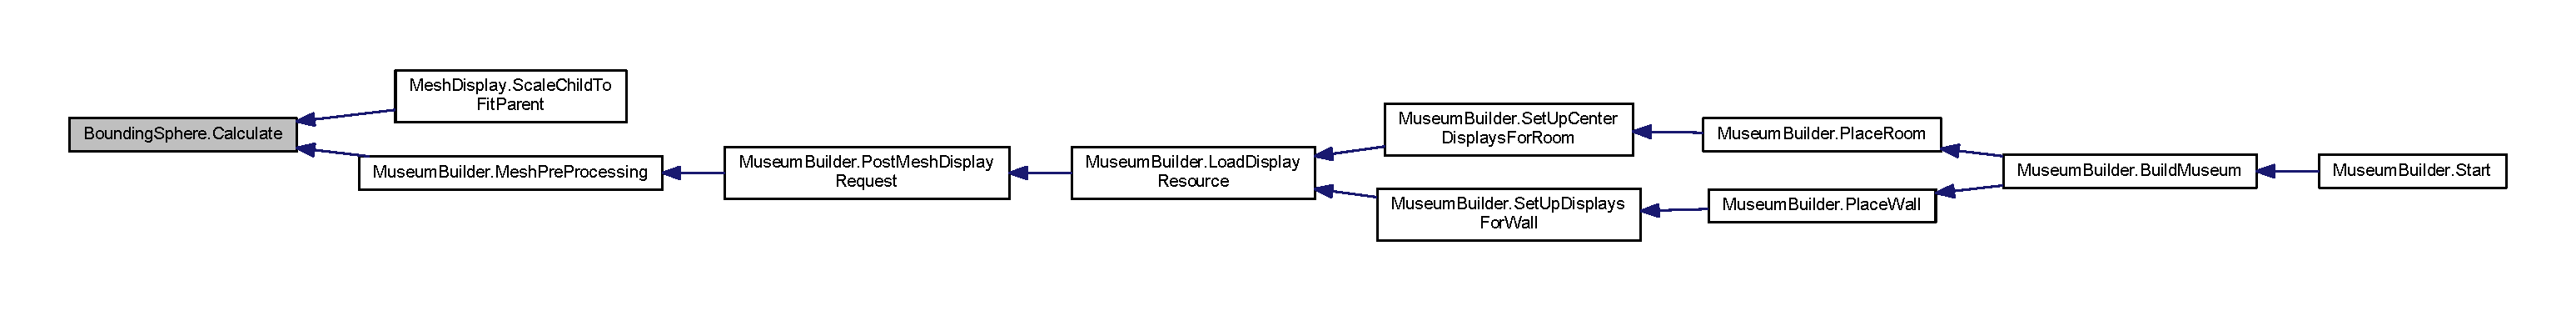
\includegraphics[width=350pt]{class_bounding_sphere_a29c277d13a701089666b94fabf3c87d6_icgraph}
\end{center}
\end{figure}


\subsection{Member Data Documentation}
\mbox{\Hypertarget{class_bounding_sphere_a0996d0f450c5e7fcca8446ebbd8ddc20}\label{class_bounding_sphere_a0996d0f450c5e7fcca8446ebbd8ddc20}} 
\index{Bounding\+Sphere@{Bounding\+Sphere}!center@{center}}
\index{center@{center}!Bounding\+Sphere@{Bounding\+Sphere}}
\subsubsection{\texorpdfstring{center}{center}}
{\footnotesize\ttfamily Vector3 Bounding\+Sphere.\+center}



center of the bounding sphre 

\mbox{\Hypertarget{class_bounding_sphere_ad507cd54bc4021617024c2545fe9379c}\label{class_bounding_sphere_ad507cd54bc4021617024c2545fe9379c}} 
\index{Bounding\+Sphere@{Bounding\+Sphere}!radius@{radius}}
\index{radius@{radius}!Bounding\+Sphere@{Bounding\+Sphere}}
\subsubsection{\texorpdfstring{radius}{radius}}
{\footnotesize\ttfamily float Bounding\+Sphere.\+radius}



radius of bounding sphere 



The documentation for this class was generated from the following file\+:\begin{DoxyCompactItemize}
\item 
C\+:/\+Unity\+Projects/\+Virt\+Muse/\+Room\+Gen\+Prototype/\+Assets/\+Scripts/\+Utility/\mbox{\hyperlink{_bounding_sphere_8cs}{Bounding\+Sphere.\+cs}}\end{DoxyCompactItemize}

\hypertarget{class_center_image_display}{}\section{Center\+Image\+Display Class Reference}
\label{class_center_image_display}\index{Center\+Image\+Display@{Center\+Image\+Display}}


Inheritance diagram for Center\+Image\+Display\+:
\nopagebreak
\begin{figure}[H]
\begin{center}
\leavevmode
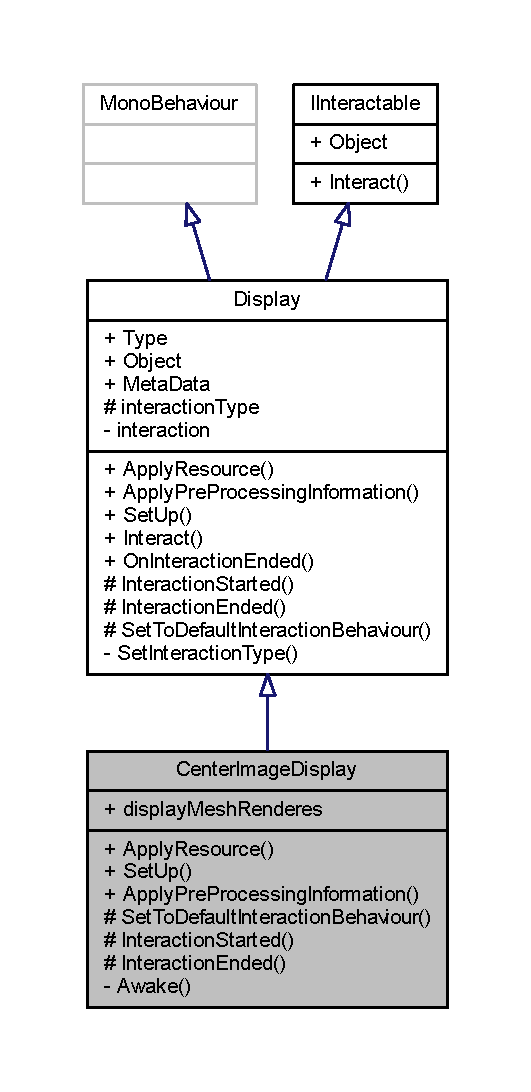
\includegraphics[width=250pt]{class_center_image_display__inherit__graph}
\end{center}
\end{figure}


Collaboration diagram for Center\+Image\+Display\+:
\nopagebreak
\begin{figure}[H]
\begin{center}
\leavevmode
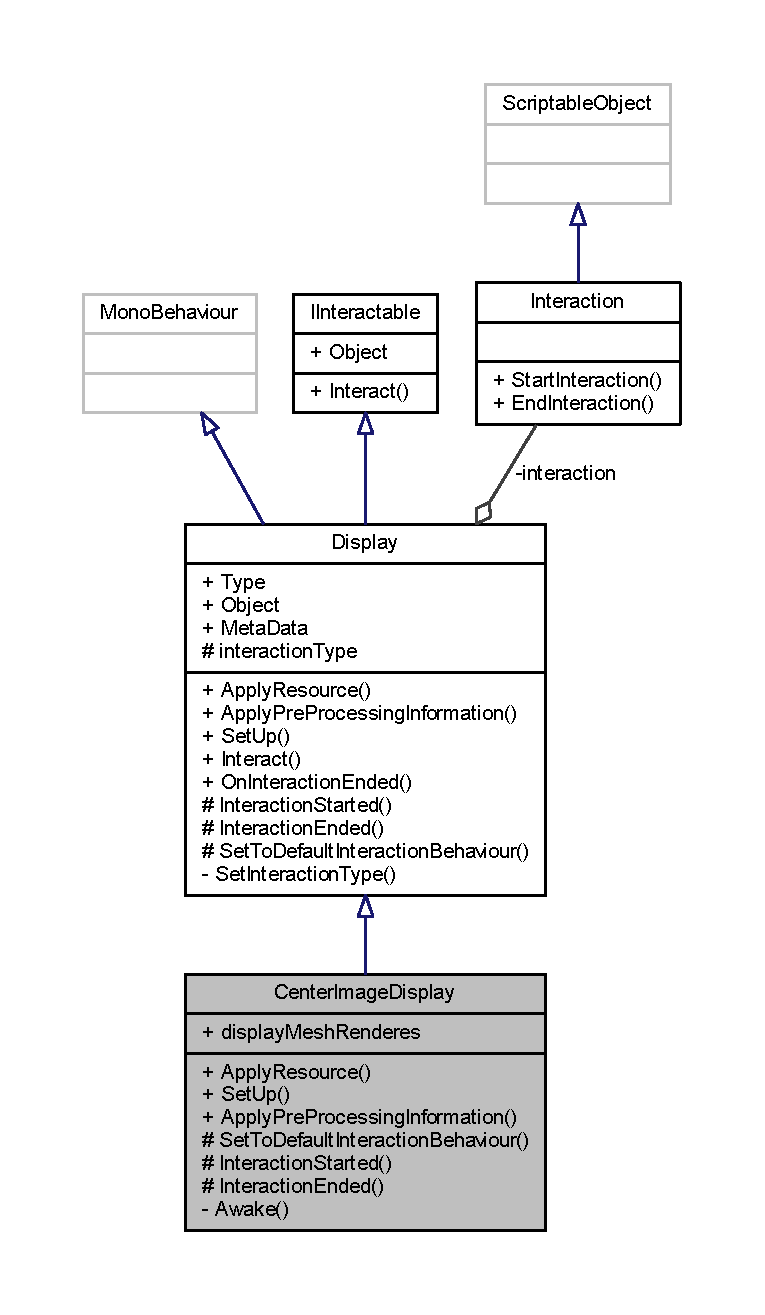
\includegraphics[width=344pt]{class_center_image_display__coll__graph}
\end{center}
\end{figure}
\subsection*{Public Member Functions}
\begin{DoxyCompactItemize}
\item 
override void \mbox{\hyperlink{class_center_image_display_a140b8b82522c1aedb473b3cd532dcd34}{Apply\+Resource}} (\mbox{\hyperlink{class_base_display_resource}{Base\+Display\+Resource}} resource)
\begin{DoxyCompactList}\small\item\em Applies a resource to a display \end{DoxyCompactList}\item 
override void \mbox{\hyperlink{class_center_image_display_a3da996020c7d8abcd24f35660945703a}{Set\+Up}} (\mbox{\hyperlink{class_museum_display_info}{Museum\+Display\+Info}} disp\+Info, Game\+Object parent)
\begin{DoxyCompactList}\small\item\em Set up the display in the museum, position and rotation \end{DoxyCompactList}\item 
override void \mbox{\hyperlink{class_center_image_display_af746f7d72e82809aaa0b5b5bf0ad2cc0}{Apply\+Pre\+Processing\+Information}} (\mbox{\hyperlink{class_pre_processing_game_object_information}{Pre\+Processing\+Game\+Object\+Information}} info)
\end{DoxyCompactItemize}
\subsection*{Public Attributes}
\begin{DoxyCompactItemize}
\item 
Raw\+Image \mbox{[}$\,$\mbox{]} \mbox{\hyperlink{class_center_image_display_afd5ccf58dcdcddc7592026ee840cf55d}{display\+Mesh\+Renderes}}
\begin{DoxyCompactList}\small\item\em the mesh renderes on all sides of the pillar \end{DoxyCompactList}\end{DoxyCompactItemize}
\subsection*{Protected Member Functions}
\begin{DoxyCompactItemize}
\item 
override System.\+Type \mbox{\hyperlink{class_center_image_display_ac6ddf9c8df99ff76c0f508ba4e45a217}{Set\+To\+Default\+Interaction\+Behaviour}} ()
\begin{DoxyCompactList}\small\item\em if the wanted behaviour is not possible or not exitent the behaviour will be set to this default \end{DoxyCompactList}\item 
override void \mbox{\hyperlink{class_center_image_display_a2944541a38bcc65b7fff15200c9f0fc3}{Interaction\+Started}} ()
\begin{DoxyCompactList}\small\item\em called when interaction with this display started used to maybe disable anything on the display gamobject if needed \end{DoxyCompactList}\item 
override void \mbox{\hyperlink{class_center_image_display_ac78f5ea36aa445bb3d12124f1baf814d}{Interaction\+Ended}} ()
\begin{DoxyCompactList}\small\item\em called when an interaction ends used to reactivate any component deactivated during the interaction \end{DoxyCompactList}\end{DoxyCompactItemize}
\subsection*{Private Member Functions}
\begin{DoxyCompactItemize}
\item 
void \mbox{\hyperlink{class_center_image_display_a413c4767daa6cca041577ba63eb3b8d5}{Awake}} ()
\end{DoxyCompactItemize}
\subsection*{Additional Inherited Members}


\subsection{Member Function Documentation}
\mbox{\Hypertarget{class_center_image_display_af746f7d72e82809aaa0b5b5bf0ad2cc0}\label{class_center_image_display_af746f7d72e82809aaa0b5b5bf0ad2cc0}} 
\index{Center\+Image\+Display@{Center\+Image\+Display}!Apply\+Pre\+Processing\+Information@{Apply\+Pre\+Processing\+Information}}
\index{Apply\+Pre\+Processing\+Information@{Apply\+Pre\+Processing\+Information}!Center\+Image\+Display@{Center\+Image\+Display}}
\subsubsection{\texorpdfstring{Apply\+Pre\+Processing\+Information()}{ApplyPreProcessingInformation()}}
{\footnotesize\ttfamily override void Center\+Image\+Display.\+Apply\+Pre\+Processing\+Information (\begin{DoxyParamCaption}\item[{\mbox{\hyperlink{class_pre_processing_game_object_information}{Pre\+Processing\+Game\+Object\+Information}}}]{info }\end{DoxyParamCaption})\hspace{0.3cm}{\ttfamily [virtual]}}



Implements \mbox{\hyperlink{class_display_ab9cd24c11c43dd87bc50e85a8e9e4c31}{Display}}.

\mbox{\Hypertarget{class_center_image_display_a140b8b82522c1aedb473b3cd532dcd34}\label{class_center_image_display_a140b8b82522c1aedb473b3cd532dcd34}} 
\index{Center\+Image\+Display@{Center\+Image\+Display}!Apply\+Resource@{Apply\+Resource}}
\index{Apply\+Resource@{Apply\+Resource}!Center\+Image\+Display@{Center\+Image\+Display}}
\subsubsection{\texorpdfstring{Apply\+Resource()}{ApplyResource()}}
{\footnotesize\ttfamily override void Center\+Image\+Display.\+Apply\+Resource (\begin{DoxyParamCaption}\item[{\mbox{\hyperlink{class_base_display_resource}{Base\+Display\+Resource}}}]{resource }\end{DoxyParamCaption})\hspace{0.3cm}{\ttfamily [virtual]}}



Applies a resource to a display 


\begin{DoxyParams}{Parameters}
{\em obj} & \\
\hline
\end{DoxyParams}


Reimplemented from \mbox{\hyperlink{class_display_a811157ddb42ae4d72f690457a08711d3}{Display}}.

\mbox{\Hypertarget{class_center_image_display_a413c4767daa6cca041577ba63eb3b8d5}\label{class_center_image_display_a413c4767daa6cca041577ba63eb3b8d5}} 
\index{Center\+Image\+Display@{Center\+Image\+Display}!Awake@{Awake}}
\index{Awake@{Awake}!Center\+Image\+Display@{Center\+Image\+Display}}
\subsubsection{\texorpdfstring{Awake()}{Awake()}}
{\footnotesize\ttfamily void Center\+Image\+Display.\+Awake (\begin{DoxyParamCaption}{ }\end{DoxyParamCaption})\hspace{0.3cm}{\ttfamily [private]}}

\mbox{\Hypertarget{class_center_image_display_ac78f5ea36aa445bb3d12124f1baf814d}\label{class_center_image_display_ac78f5ea36aa445bb3d12124f1baf814d}} 
\index{Center\+Image\+Display@{Center\+Image\+Display}!Interaction\+Ended@{Interaction\+Ended}}
\index{Interaction\+Ended@{Interaction\+Ended}!Center\+Image\+Display@{Center\+Image\+Display}}
\subsubsection{\texorpdfstring{Interaction\+Ended()}{InteractionEnded()}}
{\footnotesize\ttfamily override void Center\+Image\+Display.\+Interaction\+Ended (\begin{DoxyParamCaption}{ }\end{DoxyParamCaption})\hspace{0.3cm}{\ttfamily [protected]}, {\ttfamily [virtual]}}



called when an interaction ends used to reactivate any component deactivated during the interaction 



Implements \mbox{\hyperlink{class_display_a6fd38485267e1b78f1d1dfb589ec4ae0}{Display}}.

\mbox{\Hypertarget{class_center_image_display_a2944541a38bcc65b7fff15200c9f0fc3}\label{class_center_image_display_a2944541a38bcc65b7fff15200c9f0fc3}} 
\index{Center\+Image\+Display@{Center\+Image\+Display}!Interaction\+Started@{Interaction\+Started}}
\index{Interaction\+Started@{Interaction\+Started}!Center\+Image\+Display@{Center\+Image\+Display}}
\subsubsection{\texorpdfstring{Interaction\+Started()}{InteractionStarted()}}
{\footnotesize\ttfamily override void Center\+Image\+Display.\+Interaction\+Started (\begin{DoxyParamCaption}{ }\end{DoxyParamCaption})\hspace{0.3cm}{\ttfamily [protected]}, {\ttfamily [virtual]}}



called when interaction with this display started used to maybe disable anything on the display gamobject if needed 



Implements \mbox{\hyperlink{class_display_a21c51fcf185403197a78a5acfd2065de}{Display}}.

\mbox{\Hypertarget{class_center_image_display_ac6ddf9c8df99ff76c0f508ba4e45a217}\label{class_center_image_display_ac6ddf9c8df99ff76c0f508ba4e45a217}} 
\index{Center\+Image\+Display@{Center\+Image\+Display}!Set\+To\+Default\+Interaction\+Behaviour@{Set\+To\+Default\+Interaction\+Behaviour}}
\index{Set\+To\+Default\+Interaction\+Behaviour@{Set\+To\+Default\+Interaction\+Behaviour}!Center\+Image\+Display@{Center\+Image\+Display}}
\subsubsection{\texorpdfstring{Set\+To\+Default\+Interaction\+Behaviour()}{SetToDefaultInteractionBehaviour()}}
{\footnotesize\ttfamily override System.\+Type Center\+Image\+Display.\+Set\+To\+Default\+Interaction\+Behaviour (\begin{DoxyParamCaption}{ }\end{DoxyParamCaption})\hspace{0.3cm}{\ttfamily [protected]}, {\ttfamily [virtual]}}



if the wanted behaviour is not possible or not exitent the behaviour will be set to this default 



Implements \mbox{\hyperlink{class_display_a81f07350cf50b3924f4fe269e1b4cf17}{Display}}.

\mbox{\Hypertarget{class_center_image_display_a3da996020c7d8abcd24f35660945703a}\label{class_center_image_display_a3da996020c7d8abcd24f35660945703a}} 
\index{Center\+Image\+Display@{Center\+Image\+Display}!Set\+Up@{Set\+Up}}
\index{Set\+Up@{Set\+Up}!Center\+Image\+Display@{Center\+Image\+Display}}
\subsubsection{\texorpdfstring{Set\+Up()}{SetUp()}}
{\footnotesize\ttfamily override void Center\+Image\+Display.\+Set\+Up (\begin{DoxyParamCaption}\item[{\mbox{\hyperlink{class_museum_display_info}{Museum\+Display\+Info}}}]{disp\+Info,  }\item[{Game\+Object}]{parent }\end{DoxyParamCaption})\hspace{0.3cm}{\ttfamily [virtual]}}



Set up the display in the museum, position and rotation 


\begin{DoxyParams}{Parameters}
{\em disp\+Info} & \\
\hline
{\em parent} & \\
\hline
\end{DoxyParams}


Implements \mbox{\hyperlink{class_display_a57325251fbeac943cd48520e50f0bec4}{Display}}.



\subsection{Member Data Documentation}
\mbox{\Hypertarget{class_center_image_display_afd5ccf58dcdcddc7592026ee840cf55d}\label{class_center_image_display_afd5ccf58dcdcddc7592026ee840cf55d}} 
\index{Center\+Image\+Display@{Center\+Image\+Display}!display\+Mesh\+Renderes@{display\+Mesh\+Renderes}}
\index{display\+Mesh\+Renderes@{display\+Mesh\+Renderes}!Center\+Image\+Display@{Center\+Image\+Display}}
\subsubsection{\texorpdfstring{display\+Mesh\+Renderes}{displayMeshRenderes}}
{\footnotesize\ttfamily Raw\+Image \mbox{[}$\,$\mbox{]} Center\+Image\+Display.\+display\+Mesh\+Renderes}



the mesh renderes on all sides of the pillar 



The documentation for this class was generated from the following file\+:\begin{DoxyCompactItemize}
\item 
C\+:/\+Unity\+Projects/\+Virt\+Muse/\+Room\+Gen\+Prototype/\+Assets/\+Scripts/\+Displays/\mbox{\hyperlink{_center_image_display_8cs}{Center\+Image\+Display.\+cs}}\end{DoxyCompactItemize}

\hypertarget{class_center_mesh_display}{}\section{Center\+Mesh\+Display Class Reference}
\label{class_center_mesh_display}\index{Center\+Mesh\+Display@{Center\+Mesh\+Display}}


Inheritance diagram for Center\+Mesh\+Display\+:
\nopagebreak
\begin{figure}[H]
\begin{center}
\leavevmode
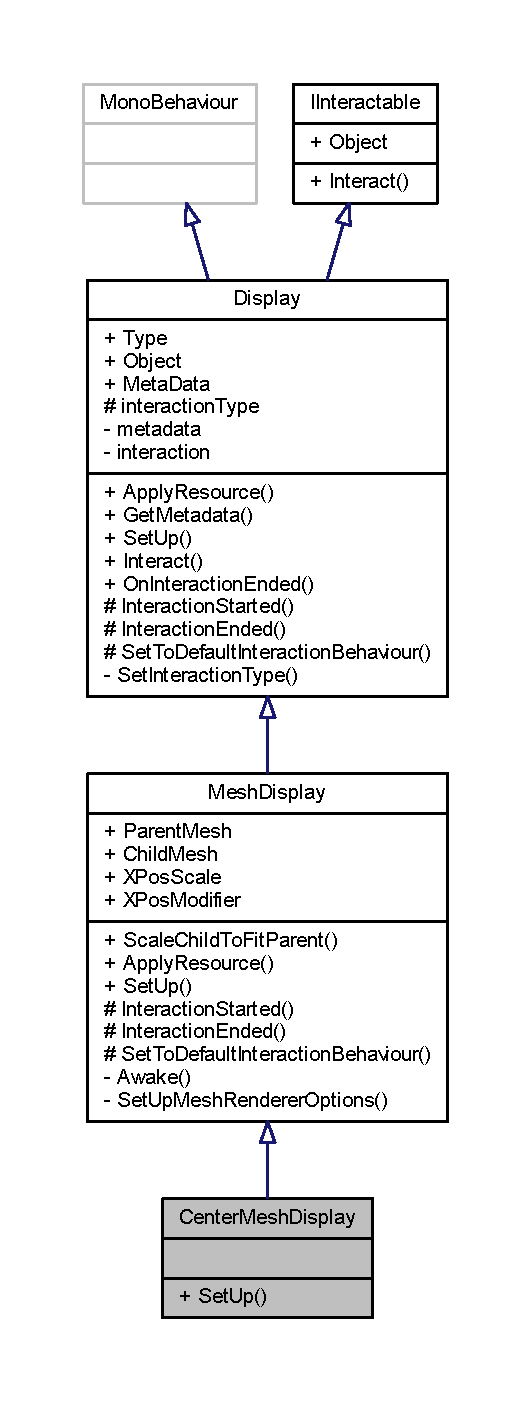
\includegraphics[height=550pt]{class_center_mesh_display__inherit__graph}
\end{center}
\end{figure}


Collaboration diagram for Center\+Mesh\+Display\+:
\nopagebreak
\begin{figure}[H]
\begin{center}
\leavevmode
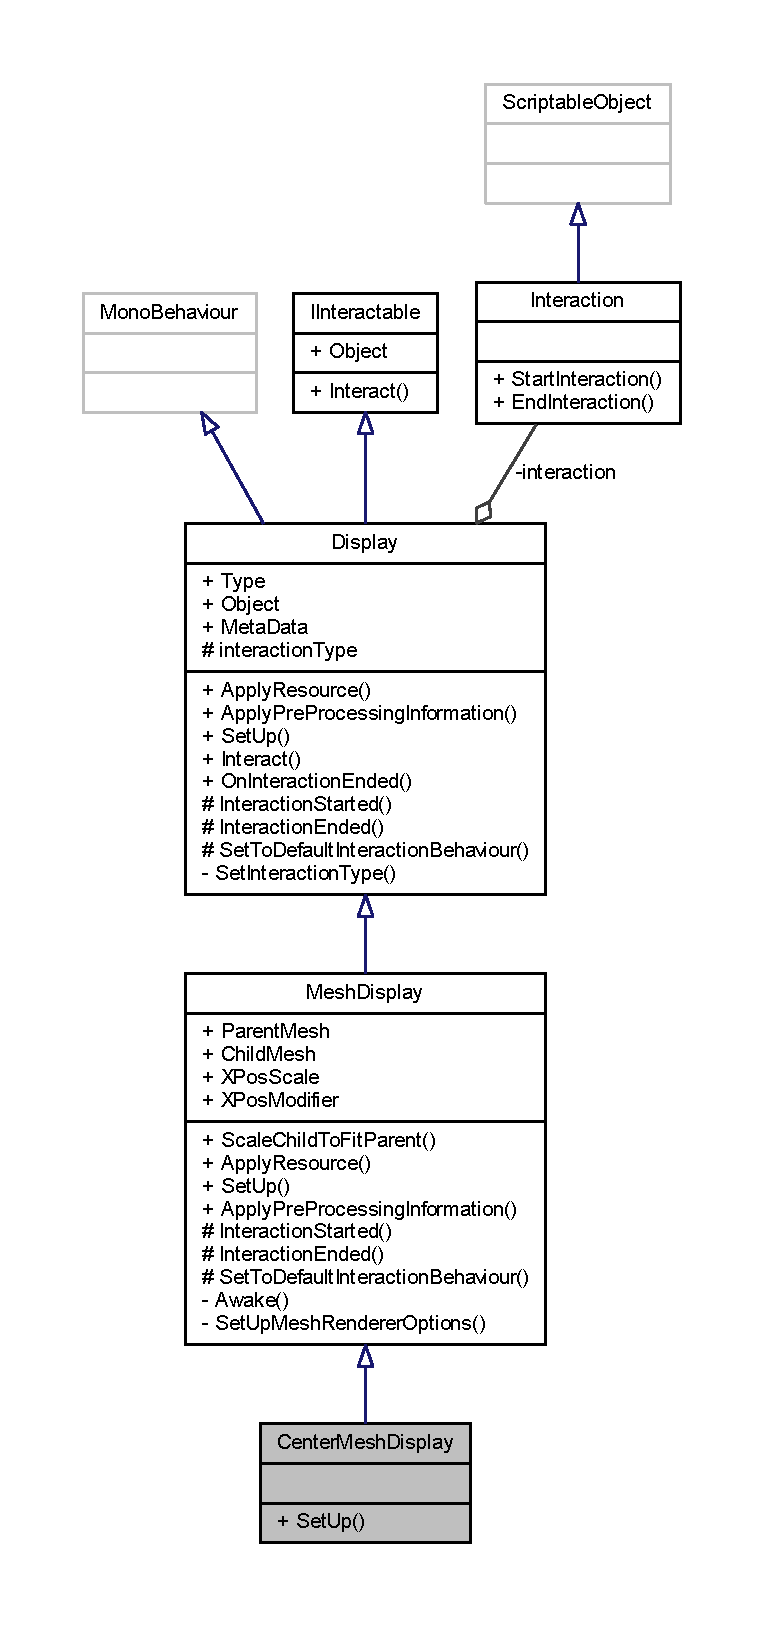
\includegraphics[height=550pt]{class_center_mesh_display__coll__graph}
\end{center}
\end{figure}
\subsection*{Public Member Functions}
\begin{DoxyCompactItemize}
\item 
override void \mbox{\hyperlink{class_center_mesh_display_a9d14ccee557aa886938d1d86ee016930}{Set\+Up}} (\mbox{\hyperlink{class_museum_display_info}{Museum\+Display\+Info}} disp\+Info, Game\+Object parent)
\begin{DoxyCompactList}\small\item\em position and parenting setup \end{DoxyCompactList}\end{DoxyCompactItemize}
\subsection*{Additional Inherited Members}


\subsection{Member Function Documentation}
\mbox{\Hypertarget{class_center_mesh_display_a9d14ccee557aa886938d1d86ee016930}\label{class_center_mesh_display_a9d14ccee557aa886938d1d86ee016930}} 
\index{Center\+Mesh\+Display@{Center\+Mesh\+Display}!Set\+Up@{Set\+Up}}
\index{Set\+Up@{Set\+Up}!Center\+Mesh\+Display@{Center\+Mesh\+Display}}
\subsubsection{\texorpdfstring{Set\+Up()}{SetUp()}}
{\footnotesize\ttfamily override void Center\+Mesh\+Display.\+Set\+Up (\begin{DoxyParamCaption}\item[{\mbox{\hyperlink{class_museum_display_info}{Museum\+Display\+Info}}}]{disp\+Info,  }\item[{Game\+Object}]{parent }\end{DoxyParamCaption})\hspace{0.3cm}{\ttfamily [virtual]}}



position and parenting setup 



Implements \mbox{\hyperlink{class_display_a57325251fbeac943cd48520e50f0bec4}{Display}}.



The documentation for this class was generated from the following file\+:\begin{DoxyCompactItemize}
\item 
C\+:/\+Unity\+Projects/\+Virt\+Muse/\+Room\+Gen\+Prototype/\+Assets/\+Scripts/\+Displays/\mbox{\hyperlink{_center_mesh_display_8cs}{Center\+Mesh\+Display.\+cs}}\end{DoxyCompactItemize}

\hypertarget{class_display}{}\section{Display Class Reference}
\label{class_display}\index{Display@{Display}}


The base class for displaying resources  




Inheritance diagram for Display\+:
\nopagebreak
\begin{figure}[H]
\begin{center}
\leavevmode
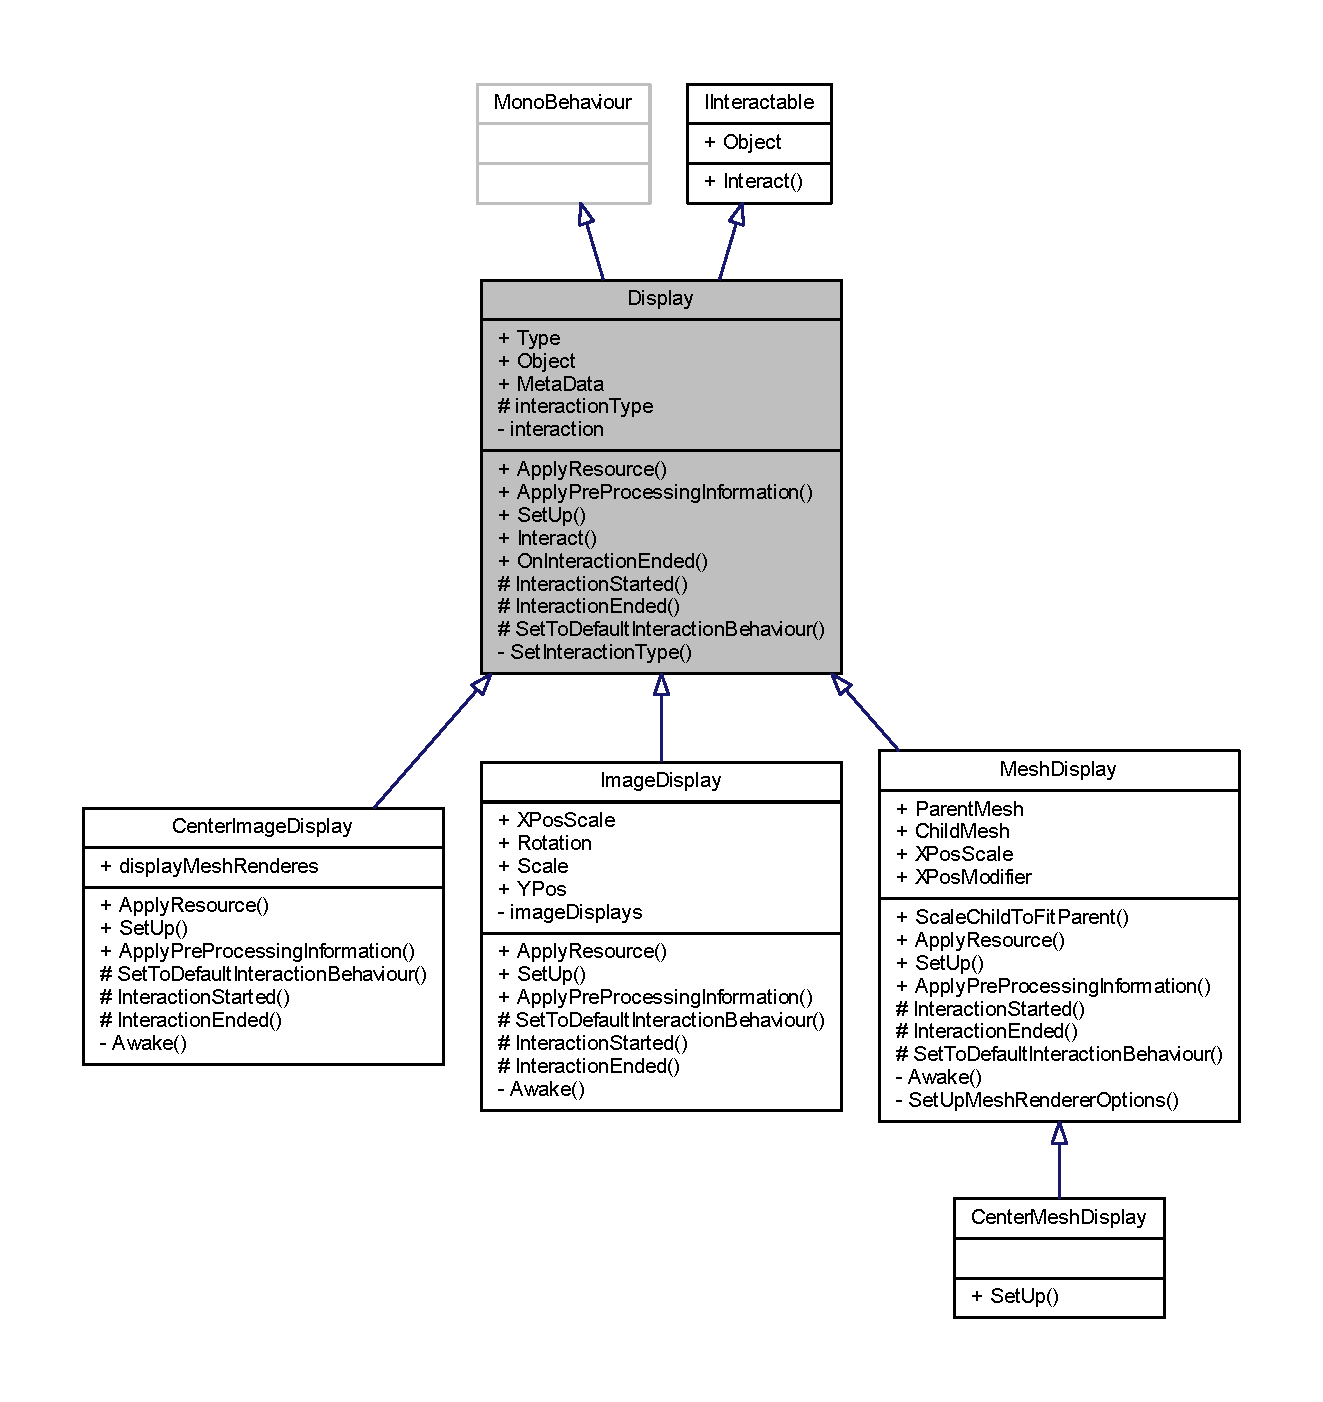
\includegraphics[width=350pt]{class_display__inherit__graph}
\end{center}
\end{figure}


Collaboration diagram for Display\+:
\nopagebreak
\begin{figure}[H]
\begin{center}
\leavevmode
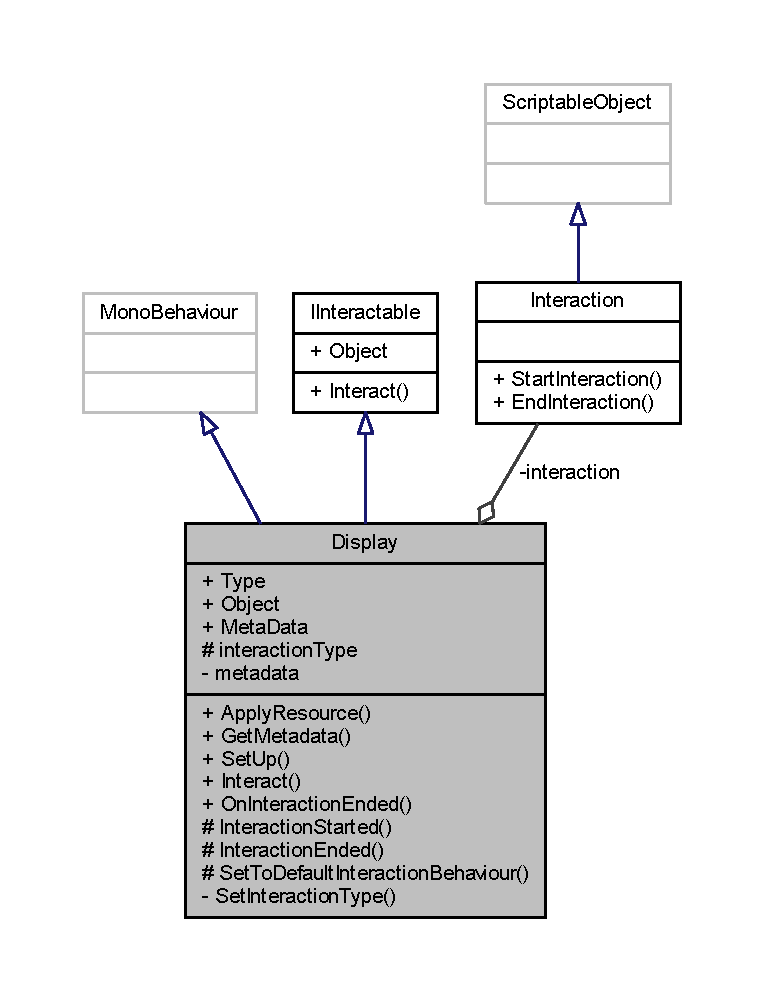
\includegraphics[width=344pt]{class_display__coll__graph}
\end{center}
\end{figure}
\subsection*{Public Types}
\begin{DoxyCompactItemize}
\item 
enum \mbox{\hyperlink{class_display_a7f7abc559192ef7e8f4a03382d3492d7}{Display\+Type}} \{ \mbox{\hyperlink{class_display_a7f7abc559192ef7e8f4a03382d3492d7a6465642df623349960f917dcf68ba989}{Display\+Type.\+Mesh\+Display}}, 
\mbox{\hyperlink{class_display_a7f7abc559192ef7e8f4a03382d3492d7a6790a36b5a0528029d4ed43891266fcb}{Display\+Type.\+Image\+Display}}
 \}
\end{DoxyCompactItemize}
\subsection*{Public Member Functions}
\begin{DoxyCompactItemize}
\item 
virtual void \mbox{\hyperlink{class_display_a811157ddb42ae4d72f690457a08711d3}{Apply\+Resource}} (\mbox{\hyperlink{class_base_display_resource}{Base\+Display\+Resource}} resource)
\begin{DoxyCompactList}\small\item\em Applies a resource to a display \end{DoxyCompactList}\item 
abstract void \mbox{\hyperlink{class_display_ab9cd24c11c43dd87bc50e85a8e9e4c31}{Apply\+Pre\+Processing\+Information}} (\mbox{\hyperlink{class_pre_processing_game_object_information}{Pre\+Processing\+Game\+Object\+Information}} info)
\item 
abstract void \mbox{\hyperlink{class_display_a57325251fbeac943cd48520e50f0bec4}{Set\+Up}} (\mbox{\hyperlink{class_museum_display_info}{Museum\+Display\+Info}} disp\+Info, Game\+Object parent)
\begin{DoxyCompactList}\small\item\em Set up the display in the museum, position and rotation \end{DoxyCompactList}\item 
void \mbox{\hyperlink{class_display_a43fc2a6f19bbf2f1bdb676392b37e921}{Interact}} (\mbox{\hyperlink{class_player}{Player}} player)
\begin{DoxyCompactList}\small\item\em called when the player interacts with this display \end{DoxyCompactList}\item 
void \mbox{\hyperlink{class_display_a29f45efdf15e97219d2c8a614d699da8}{On\+Interaction\+Ended}} (\mbox{\hyperlink{class_player_interaction_event_args}{Player\+Interaction\+Event\+Args}} arg)
\begin{DoxyCompactList}\small\item\em called from event when the interction is ended \end{DoxyCompactList}\end{DoxyCompactItemize}
\subsection*{Protected Member Functions}
\begin{DoxyCompactItemize}
\item 
abstract void \mbox{\hyperlink{class_display_a21c51fcf185403197a78a5acfd2065de}{Interaction\+Started}} ()
\begin{DoxyCompactList}\small\item\em called when interaction with this display started used to maybe disable anything on the display gamobject if needed \end{DoxyCompactList}\item 
abstract void \mbox{\hyperlink{class_display_a6fd38485267e1b78f1d1dfb589ec4ae0}{Interaction\+Ended}} ()
\begin{DoxyCompactList}\small\item\em called when an interaction ends used to reactivate any component deactivated during the interaction \end{DoxyCompactList}\item 
abstract \mbox{\hyperlink{class_display_a2c80ba13fff1fd81aaa6915b28e8c14f}{Type}} \mbox{\hyperlink{class_display_a81f07350cf50b3924f4fe269e1b4cf17}{Set\+To\+Default\+Interaction\+Behaviour}} ()
\begin{DoxyCompactList}\small\item\em if the wanted behaviour is not possible or not exitent the behaviour will be set to this default \end{DoxyCompactList}\end{DoxyCompactItemize}
\subsection*{Protected Attributes}
\begin{DoxyCompactItemize}
\item 
\mbox{\hyperlink{class_display_a2c80ba13fff1fd81aaa6915b28e8c14f}{Type}} \mbox{\hyperlink{class_display_aab913d6cfa4e9631e8129ed131e79196}{interaction\+Type}}
\begin{DoxyCompactList}\small\item\em System type of the interaction the display provides \end{DoxyCompactList}\end{DoxyCompactItemize}
\subsection*{Properties}
\begin{DoxyCompactItemize}
\item 
\mbox{\hyperlink{class_display_a7f7abc559192ef7e8f4a03382d3492d7}{Display\+Type}} \mbox{\hyperlink{class_display_a2c80ba13fff1fd81aaa6915b28e8c14f}{Type}}\hspace{0.3cm}{\ttfamily  \mbox{[}get, protected set\mbox{]}}
\begin{DoxyCompactList}\small\item\em Type of display \end{DoxyCompactList}\item 
Game\+Object \mbox{\hyperlink{class_display_a32b9644a140d330a9c51cfdbb6f6093c}{Object}}\hspace{0.3cm}{\ttfamily  \mbox{[}get\mbox{]}}
\item 
\mbox{\hyperlink{class_meta_data}{Meta\+Data}} \mbox{\hyperlink{class_display_a9ae693bcb1553822aed7ae887a65591c}{Meta\+Data}}\hspace{0.3cm}{\ttfamily  \mbox{[}get, private set\mbox{]}}
\begin{DoxyCompactList}\small\item\em the metadata that further describes the resource held by the display \end{DoxyCompactList}\end{DoxyCompactItemize}
\subsection*{Private Member Functions}
\begin{DoxyCompactItemize}
\item 
void \mbox{\hyperlink{class_display_af8aa8a663725645f431095397ad802e6}{Set\+Interaction\+Type}} (string wanted\+\_\+behaviour)
\begin{DoxyCompactList}\small\item\em sets the interaction type of this display \end{DoxyCompactList}\end{DoxyCompactItemize}
\subsection*{Private Attributes}
\begin{DoxyCompactItemize}
\item 
\mbox{\hyperlink{class_interaction}{Interaction}} \mbox{\hyperlink{class_display_af35594f083ed6dd4279183215719583f}{interaction}}
\begin{DoxyCompactList}\small\item\em the interaction that is currently taking place \end{DoxyCompactList}\end{DoxyCompactItemize}


\subsection{Detailed Description}
The base class for displaying resources 



\subsection{Member Enumeration Documentation}
\mbox{\Hypertarget{class_display_a7f7abc559192ef7e8f4a03382d3492d7}\label{class_display_a7f7abc559192ef7e8f4a03382d3492d7}} 
\index{Display@{Display}!Display\+Type@{Display\+Type}}
\index{Display\+Type@{Display\+Type}!Display@{Display}}
\subsubsection{\texorpdfstring{Display\+Type}{DisplayType}}
{\footnotesize\ttfamily enum \mbox{\hyperlink{class_display_a7f7abc559192ef7e8f4a03382d3492d7}{Display.\+Display\+Type}}\hspace{0.3cm}{\ttfamily [strong]}}

\begin{DoxyEnumFields}{Enumerator}
\raisebox{\heightof{T}}[0pt][0pt]{\index{Mesh\+Display@{Mesh\+Display}!Display@{Display}}\index{Display@{Display}!Mesh\+Display@{Mesh\+Display}}}\mbox{\Hypertarget{class_display_a7f7abc559192ef7e8f4a03382d3492d7a6465642df623349960f917dcf68ba989}\label{class_display_a7f7abc559192ef7e8f4a03382d3492d7a6465642df623349960f917dcf68ba989}} 
Mesh\+Display&\\
\hline

\raisebox{\heightof{T}}[0pt][0pt]{\index{Image\+Display@{Image\+Display}!Display@{Display}}\index{Display@{Display}!Image\+Display@{Image\+Display}}}\mbox{\Hypertarget{class_display_a7f7abc559192ef7e8f4a03382d3492d7a6790a36b5a0528029d4ed43891266fcb}\label{class_display_a7f7abc559192ef7e8f4a03382d3492d7a6790a36b5a0528029d4ed43891266fcb}} 
Image\+Display&\\
\hline

\end{DoxyEnumFields}


\subsection{Member Function Documentation}
\mbox{\Hypertarget{class_display_ab9cd24c11c43dd87bc50e85a8e9e4c31}\label{class_display_ab9cd24c11c43dd87bc50e85a8e9e4c31}} 
\index{Display@{Display}!Apply\+Pre\+Processing\+Information@{Apply\+Pre\+Processing\+Information}}
\index{Apply\+Pre\+Processing\+Information@{Apply\+Pre\+Processing\+Information}!Display@{Display}}
\subsubsection{\texorpdfstring{Apply\+Pre\+Processing\+Information()}{ApplyPreProcessingInformation()}}
{\footnotesize\ttfamily abstract void Display.\+Apply\+Pre\+Processing\+Information (\begin{DoxyParamCaption}\item[{\mbox{\hyperlink{class_pre_processing_game_object_information}{Pre\+Processing\+Game\+Object\+Information}}}]{info }\end{DoxyParamCaption})\hspace{0.3cm}{\ttfamily [pure virtual]}}



Implemented in \mbox{\hyperlink{class_mesh_display_ab52b4d43c963b3bef383e2eebd1e4115}{Mesh\+Display}}, \mbox{\hyperlink{class_image_display_a0ad82d85f6c4ec5eabb65afa1ae72bc1}{Image\+Display}}, and \mbox{\hyperlink{class_center_image_display_af746f7d72e82809aaa0b5b5bf0ad2cc0}{Center\+Image\+Display}}.

Here is the caller graph for this function\+:
\nopagebreak
\begin{figure}[H]
\begin{center}
\leavevmode
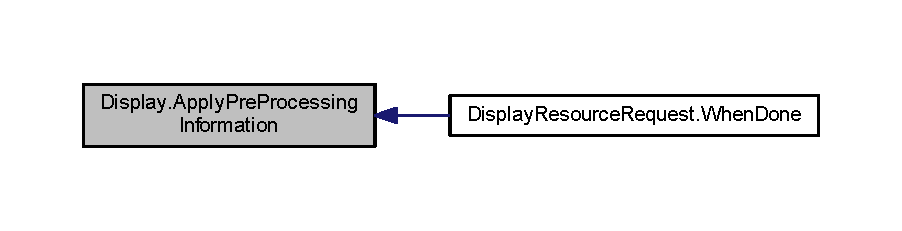
\includegraphics[width=350pt]{class_display_ab9cd24c11c43dd87bc50e85a8e9e4c31_icgraph}
\end{center}
\end{figure}
\mbox{\Hypertarget{class_display_a811157ddb42ae4d72f690457a08711d3}\label{class_display_a811157ddb42ae4d72f690457a08711d3}} 
\index{Display@{Display}!Apply\+Resource@{Apply\+Resource}}
\index{Apply\+Resource@{Apply\+Resource}!Display@{Display}}
\subsubsection{\texorpdfstring{Apply\+Resource()}{ApplyResource()}}
{\footnotesize\ttfamily virtual void Display.\+Apply\+Resource (\begin{DoxyParamCaption}\item[{\mbox{\hyperlink{class_base_display_resource}{Base\+Display\+Resource}}}]{resource }\end{DoxyParamCaption})\hspace{0.3cm}{\ttfamily [virtual]}}



Applies a resource to a display 


\begin{DoxyParams}{Parameters}
{\em obj} & \\
\hline
\end{DoxyParams}


Reimplemented in \mbox{\hyperlink{class_mesh_display_ab9a24f407a8ff995658097a98242095e}{Mesh\+Display}}, \mbox{\hyperlink{class_image_display_ab4cae8c66db7e7d77ab117fe24e63980}{Image\+Display}}, and \mbox{\hyperlink{class_center_image_display_a140b8b82522c1aedb473b3cd532dcd34}{Center\+Image\+Display}}.

Here is the call graph for this function\+:
\nopagebreak
\begin{figure}[H]
\begin{center}
\leavevmode
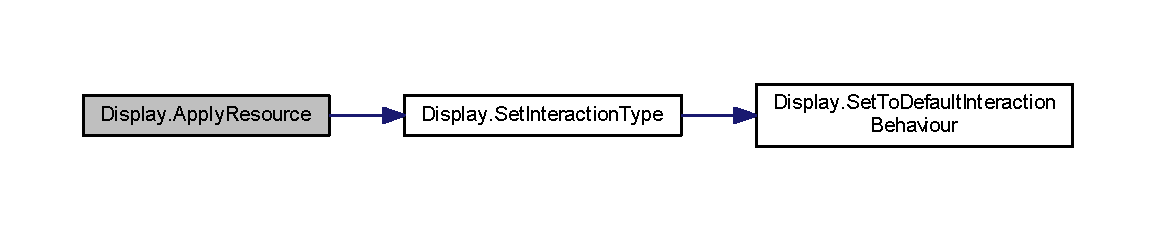
\includegraphics[width=350pt]{class_display_a811157ddb42ae4d72f690457a08711d3_cgraph}
\end{center}
\end{figure}
Here is the caller graph for this function\+:
\nopagebreak
\begin{figure}[H]
\begin{center}
\leavevmode
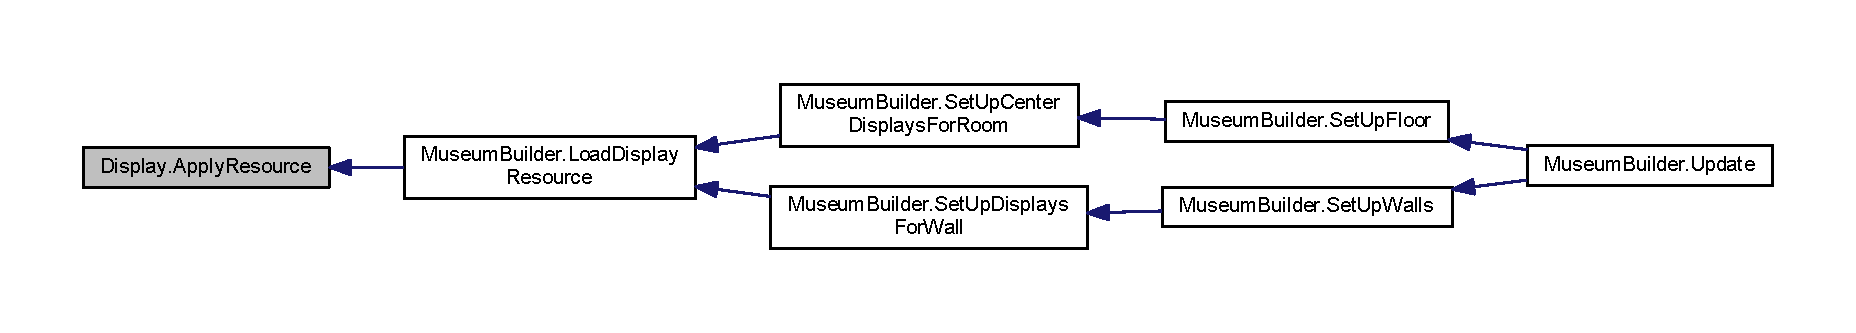
\includegraphics[width=350pt]{class_display_a811157ddb42ae4d72f690457a08711d3_icgraph}
\end{center}
\end{figure}
\mbox{\Hypertarget{class_display_a43fc2a6f19bbf2f1bdb676392b37e921}\label{class_display_a43fc2a6f19bbf2f1bdb676392b37e921}} 
\index{Display@{Display}!Interact@{Interact}}
\index{Interact@{Interact}!Display@{Display}}
\subsubsection{\texorpdfstring{Interact()}{Interact()}}
{\footnotesize\ttfamily void Display.\+Interact (\begin{DoxyParamCaption}\item[{\mbox{\hyperlink{class_player}{Player}}}]{player }\end{DoxyParamCaption})}



called when the player interacts with this display 


\begin{DoxyParams}{Parameters}
{\em player} & \\
\hline
\end{DoxyParams}


Implements \mbox{\hyperlink{interface_i_interactable_a736e28381ac0e7ca60f5fae2feb95afe}{I\+Interactable}}.

Here is the call graph for this function\+:
\nopagebreak
\begin{figure}[H]
\begin{center}
\leavevmode
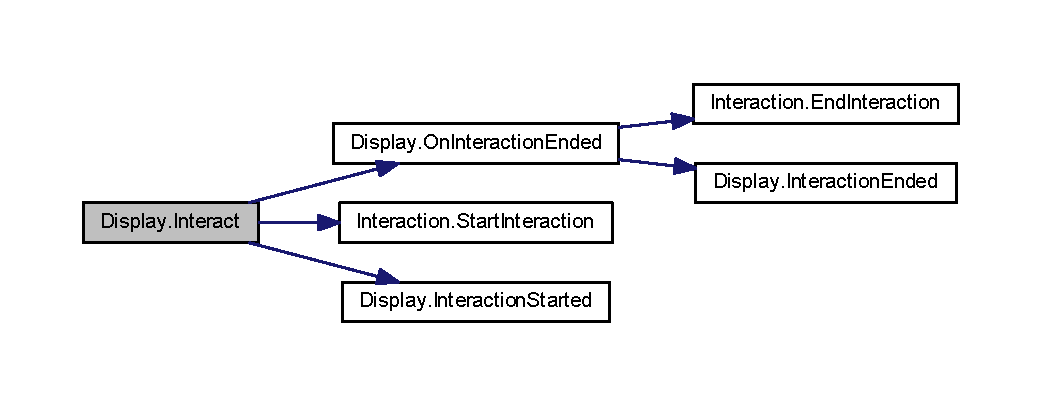
\includegraphics[width=350pt]{class_display_a43fc2a6f19bbf2f1bdb676392b37e921_cgraph}
\end{center}
\end{figure}
\mbox{\Hypertarget{class_display_a6fd38485267e1b78f1d1dfb589ec4ae0}\label{class_display_a6fd38485267e1b78f1d1dfb589ec4ae0}} 
\index{Display@{Display}!Interaction\+Ended@{Interaction\+Ended}}
\index{Interaction\+Ended@{Interaction\+Ended}!Display@{Display}}
\subsubsection{\texorpdfstring{Interaction\+Ended()}{InteractionEnded()}}
{\footnotesize\ttfamily abstract void Display.\+Interaction\+Ended (\begin{DoxyParamCaption}{ }\end{DoxyParamCaption})\hspace{0.3cm}{\ttfamily [protected]}, {\ttfamily [pure virtual]}}



called when an interaction ends used to reactivate any component deactivated during the interaction 



Implemented in \mbox{\hyperlink{class_mesh_display_a23f7ab8b0f48536940ad1cc2145297b3}{Mesh\+Display}}, \mbox{\hyperlink{class_image_display_a94c5928ef81449c37740d0bd0a8f4062}{Image\+Display}}, and \mbox{\hyperlink{class_center_image_display_ac78f5ea36aa445bb3d12124f1baf814d}{Center\+Image\+Display}}.

Here is the caller graph for this function\+:
\nopagebreak
\begin{figure}[H]
\begin{center}
\leavevmode
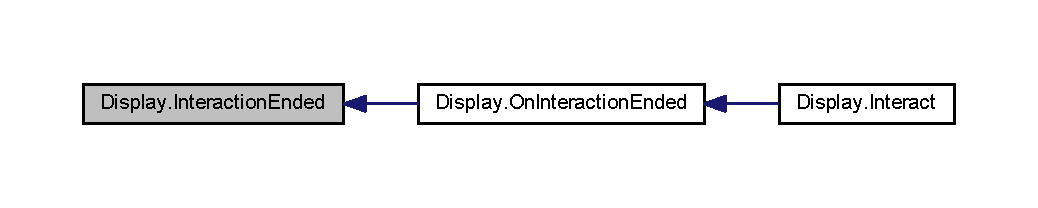
\includegraphics[width=350pt]{class_display_a6fd38485267e1b78f1d1dfb589ec4ae0_icgraph}
\end{center}
\end{figure}
\mbox{\Hypertarget{class_display_a21c51fcf185403197a78a5acfd2065de}\label{class_display_a21c51fcf185403197a78a5acfd2065de}} 
\index{Display@{Display}!Interaction\+Started@{Interaction\+Started}}
\index{Interaction\+Started@{Interaction\+Started}!Display@{Display}}
\subsubsection{\texorpdfstring{Interaction\+Started()}{InteractionStarted()}}
{\footnotesize\ttfamily abstract void Display.\+Interaction\+Started (\begin{DoxyParamCaption}{ }\end{DoxyParamCaption})\hspace{0.3cm}{\ttfamily [protected]}, {\ttfamily [pure virtual]}}



called when interaction with this display started used to maybe disable anything on the display gamobject if needed 



Implemented in \mbox{\hyperlink{class_mesh_display_aa4affc65c23027c877f511fc2b8aaeb8}{Mesh\+Display}}, \mbox{\hyperlink{class_image_display_a1fdf91b09cd5329059d38033f1330ffb}{Image\+Display}}, and \mbox{\hyperlink{class_center_image_display_a2944541a38bcc65b7fff15200c9f0fc3}{Center\+Image\+Display}}.

Here is the caller graph for this function\+:
\nopagebreak
\begin{figure}[H]
\begin{center}
\leavevmode
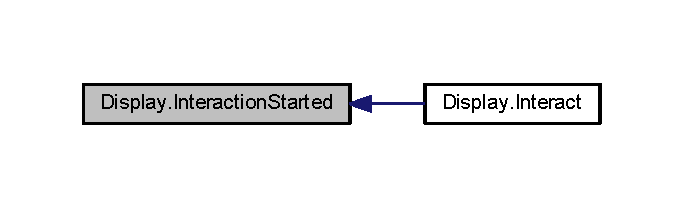
\includegraphics[width=328pt]{class_display_a21c51fcf185403197a78a5acfd2065de_icgraph}
\end{center}
\end{figure}
\mbox{\Hypertarget{class_display_a29f45efdf15e97219d2c8a614d699da8}\label{class_display_a29f45efdf15e97219d2c8a614d699da8}} 
\index{Display@{Display}!On\+Interaction\+Ended@{On\+Interaction\+Ended}}
\index{On\+Interaction\+Ended@{On\+Interaction\+Ended}!Display@{Display}}
\subsubsection{\texorpdfstring{On\+Interaction\+Ended()}{OnInteractionEnded()}}
{\footnotesize\ttfamily void Display.\+On\+Interaction\+Ended (\begin{DoxyParamCaption}\item[{\mbox{\hyperlink{class_player_interaction_event_args}{Player\+Interaction\+Event\+Args}}}]{arg }\end{DoxyParamCaption})}



called from event when the interction is ended 


\begin{DoxyParams}{Parameters}
{\em arg} & event arguments\\
\hline
\end{DoxyParams}
Here is the call graph for this function\+:
\nopagebreak
\begin{figure}[H]
\begin{center}
\leavevmode
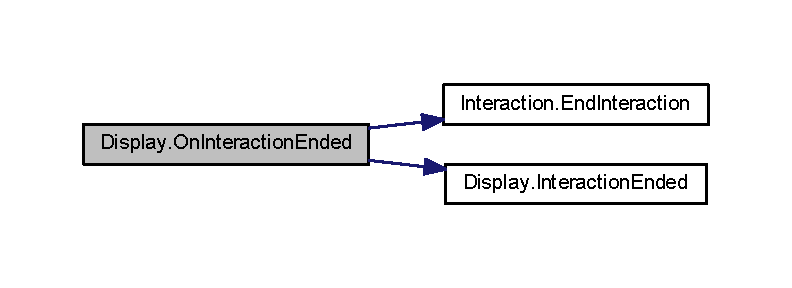
\includegraphics[width=350pt]{class_display_a29f45efdf15e97219d2c8a614d699da8_cgraph}
\end{center}
\end{figure}
Here is the caller graph for this function\+:
\nopagebreak
\begin{figure}[H]
\begin{center}
\leavevmode
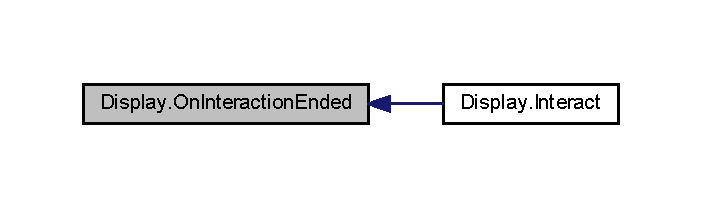
\includegraphics[width=337pt]{class_display_a29f45efdf15e97219d2c8a614d699da8_icgraph}
\end{center}
\end{figure}
\mbox{\Hypertarget{class_display_af8aa8a663725645f431095397ad802e6}\label{class_display_af8aa8a663725645f431095397ad802e6}} 
\index{Display@{Display}!Set\+Interaction\+Type@{Set\+Interaction\+Type}}
\index{Set\+Interaction\+Type@{Set\+Interaction\+Type}!Display@{Display}}
\subsubsection{\texorpdfstring{Set\+Interaction\+Type()}{SetInteractionType()}}
{\footnotesize\ttfamily void Display.\+Set\+Interaction\+Type (\begin{DoxyParamCaption}\item[{string}]{wanted\+\_\+behaviour }\end{DoxyParamCaption})\hspace{0.3cm}{\ttfamily [private]}}



sets the interaction type of this display 


\begin{DoxyParams}{Parameters}
{\em wanted\+\_\+behaviour} & the wanted behaviour\\
\hline
\end{DoxyParams}
Here is the call graph for this function\+:
\nopagebreak
\begin{figure}[H]
\begin{center}
\leavevmode
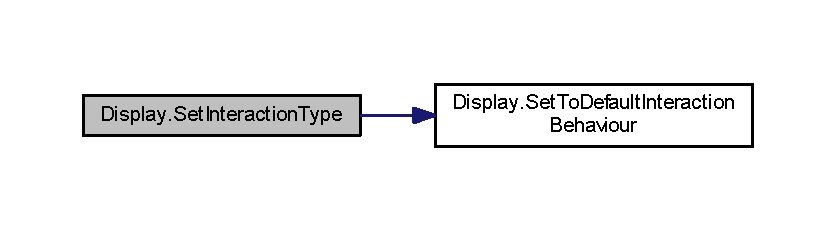
\includegraphics[width=350pt]{class_display_af8aa8a663725645f431095397ad802e6_cgraph}
\end{center}
\end{figure}
Here is the caller graph for this function\+:
\nopagebreak
\begin{figure}[H]
\begin{center}
\leavevmode
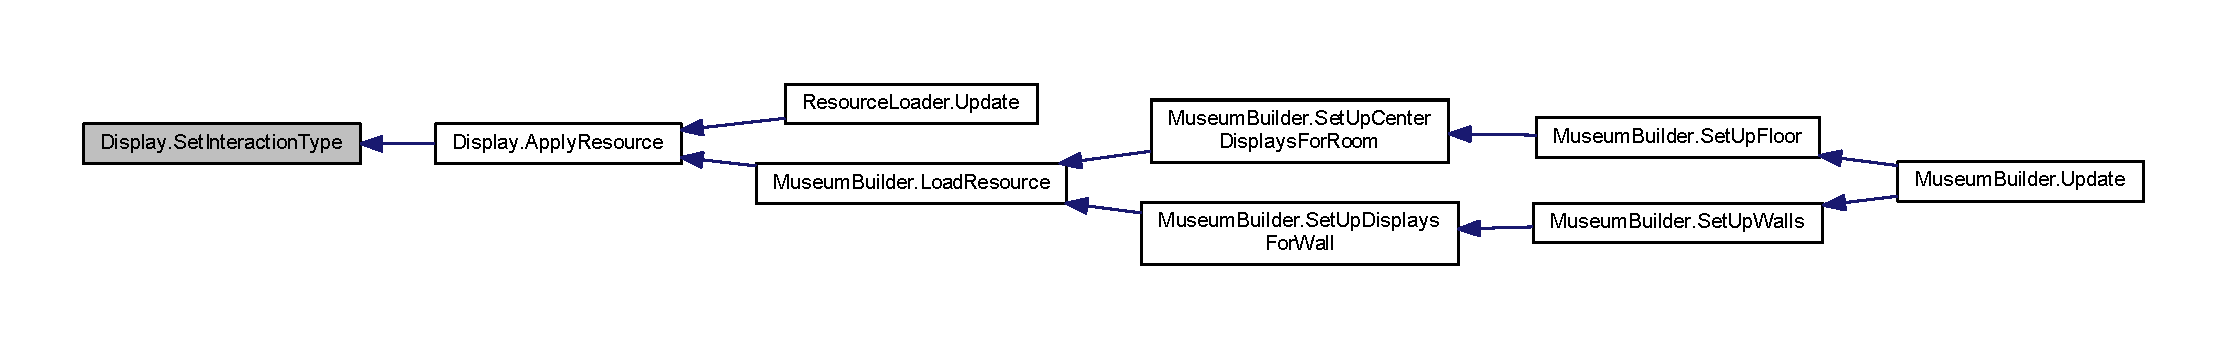
\includegraphics[width=350pt]{class_display_af8aa8a663725645f431095397ad802e6_icgraph}
\end{center}
\end{figure}
\mbox{\Hypertarget{class_display_a81f07350cf50b3924f4fe269e1b4cf17}\label{class_display_a81f07350cf50b3924f4fe269e1b4cf17}} 
\index{Display@{Display}!Set\+To\+Default\+Interaction\+Behaviour@{Set\+To\+Default\+Interaction\+Behaviour}}
\index{Set\+To\+Default\+Interaction\+Behaviour@{Set\+To\+Default\+Interaction\+Behaviour}!Display@{Display}}
\subsubsection{\texorpdfstring{Set\+To\+Default\+Interaction\+Behaviour()}{SetToDefaultInteractionBehaviour()}}
{\footnotesize\ttfamily abstract \mbox{\hyperlink{class_display_a2c80ba13fff1fd81aaa6915b28e8c14f}{Type}} Display.\+Set\+To\+Default\+Interaction\+Behaviour (\begin{DoxyParamCaption}{ }\end{DoxyParamCaption})\hspace{0.3cm}{\ttfamily [protected]}, {\ttfamily [pure virtual]}}



if the wanted behaviour is not possible or not exitent the behaviour will be set to this default 



Implemented in \mbox{\hyperlink{class_mesh_display_a8cd58e07cb9d64598c3bbc6701515d1d}{Mesh\+Display}}, \mbox{\hyperlink{class_image_display_ae975595939d76dd1db32e6f029f53ab6}{Image\+Display}}, and \mbox{\hyperlink{class_center_image_display_ac6ddf9c8df99ff76c0f508ba4e45a217}{Center\+Image\+Display}}.

Here is the caller graph for this function\+:
\nopagebreak
\begin{figure}[H]
\begin{center}
\leavevmode
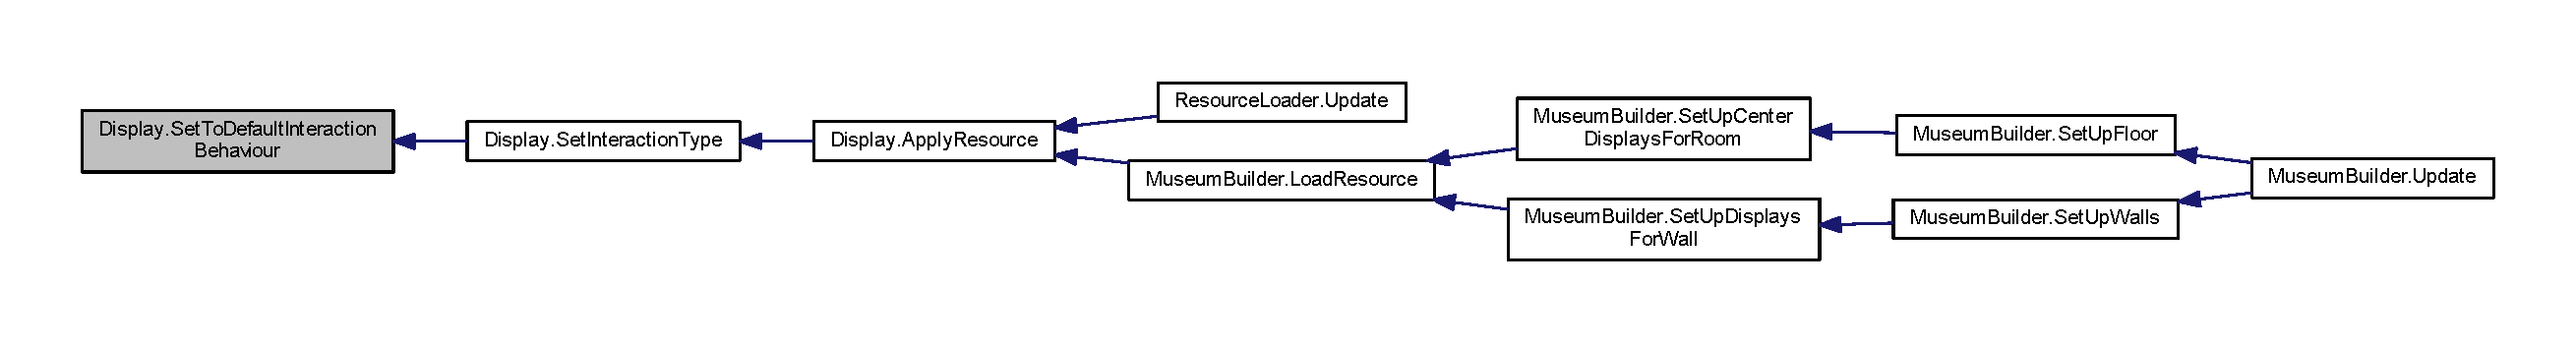
\includegraphics[width=350pt]{class_display_a81f07350cf50b3924f4fe269e1b4cf17_icgraph}
\end{center}
\end{figure}
\mbox{\Hypertarget{class_display_a57325251fbeac943cd48520e50f0bec4}\label{class_display_a57325251fbeac943cd48520e50f0bec4}} 
\index{Display@{Display}!Set\+Up@{Set\+Up}}
\index{Set\+Up@{Set\+Up}!Display@{Display}}
\subsubsection{\texorpdfstring{Set\+Up()}{SetUp()}}
{\footnotesize\ttfamily abstract void Display.\+Set\+Up (\begin{DoxyParamCaption}\item[{\mbox{\hyperlink{class_museum_display_info}{Museum\+Display\+Info}}}]{disp\+Info,  }\item[{Game\+Object}]{parent }\end{DoxyParamCaption})\hspace{0.3cm}{\ttfamily [pure virtual]}}



Set up the display in the museum, position and rotation 


\begin{DoxyParams}{Parameters}
{\em disp\+Info} & \\
\hline
{\em parent} & \\
\hline
\end{DoxyParams}


Implemented in \mbox{\hyperlink{class_mesh_display_adb19ca4d076a93df64d1c035663fce0f}{Mesh\+Display}}, \mbox{\hyperlink{class_image_display_a28fead7caeeb12490d26fae943da6a1e}{Image\+Display}}, \mbox{\hyperlink{class_center_image_display_a3da996020c7d8abcd24f35660945703a}{Center\+Image\+Display}}, and \mbox{\hyperlink{class_center_mesh_display_a9d14ccee557aa886938d1d86ee016930}{Center\+Mesh\+Display}}.

Here is the caller graph for this function\+:
\nopagebreak
\begin{figure}[H]
\begin{center}
\leavevmode
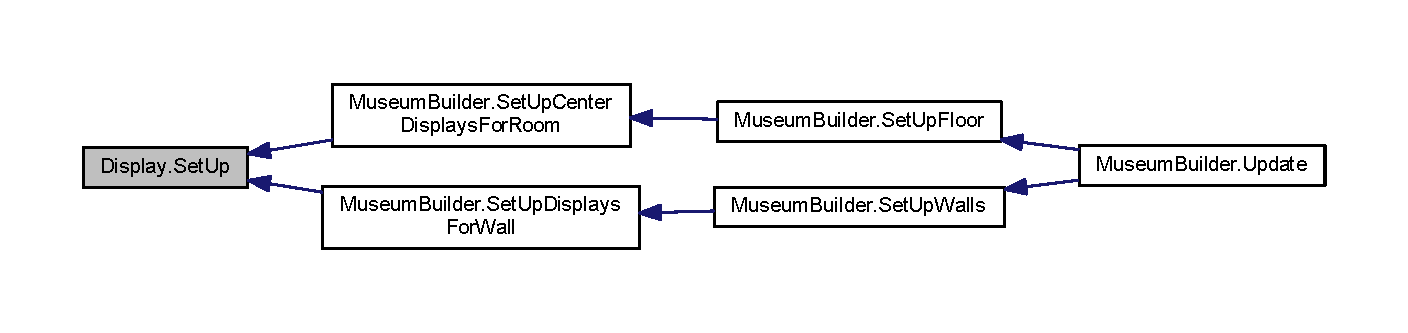
\includegraphics[width=350pt]{class_display_a57325251fbeac943cd48520e50f0bec4_icgraph}
\end{center}
\end{figure}


\subsection{Member Data Documentation}
\mbox{\Hypertarget{class_display_af35594f083ed6dd4279183215719583f}\label{class_display_af35594f083ed6dd4279183215719583f}} 
\index{Display@{Display}!interaction@{interaction}}
\index{interaction@{interaction}!Display@{Display}}
\subsubsection{\texorpdfstring{interaction}{interaction}}
{\footnotesize\ttfamily \mbox{\hyperlink{class_interaction}{Interaction}} Display.\+interaction\hspace{0.3cm}{\ttfamily [private]}}



the interaction that is currently taking place 

\mbox{\Hypertarget{class_display_aab913d6cfa4e9631e8129ed131e79196}\label{class_display_aab913d6cfa4e9631e8129ed131e79196}} 
\index{Display@{Display}!interaction\+Type@{interaction\+Type}}
\index{interaction\+Type@{interaction\+Type}!Display@{Display}}
\subsubsection{\texorpdfstring{interaction\+Type}{interactionType}}
{\footnotesize\ttfamily \mbox{\hyperlink{class_display_a2c80ba13fff1fd81aaa6915b28e8c14f}{Type}} Display.\+interaction\+Type\hspace{0.3cm}{\ttfamily [protected]}}



System type of the interaction the display provides 



\subsection{Property Documentation}
\mbox{\Hypertarget{class_display_a9ae693bcb1553822aed7ae887a65591c}\label{class_display_a9ae693bcb1553822aed7ae887a65591c}} 
\index{Display@{Display}!Meta\+Data@{Meta\+Data}}
\index{Meta\+Data@{Meta\+Data}!Display@{Display}}
\subsubsection{\texorpdfstring{Meta\+Data}{MetaData}}
{\footnotesize\ttfamily \mbox{\hyperlink{class_meta_data}{Meta\+Data}} Display.\+Meta\+Data\hspace{0.3cm}{\ttfamily [get]}, {\ttfamily [private set]}}



the metadata that further describes the resource held by the display 

\mbox{\Hypertarget{class_display_a32b9644a140d330a9c51cfdbb6f6093c}\label{class_display_a32b9644a140d330a9c51cfdbb6f6093c}} 
\index{Display@{Display}!Object@{Object}}
\index{Object@{Object}!Display@{Display}}
\subsubsection{\texorpdfstring{Object}{Object}}
{\footnotesize\ttfamily Game\+Object Display.\+Object\hspace{0.3cm}{\ttfamily [get]}}

\mbox{\Hypertarget{class_display_a2c80ba13fff1fd81aaa6915b28e8c14f}\label{class_display_a2c80ba13fff1fd81aaa6915b28e8c14f}} 
\index{Display@{Display}!Type@{Type}}
\index{Type@{Type}!Display@{Display}}
\subsubsection{\texorpdfstring{Type}{Type}}
{\footnotesize\ttfamily \mbox{\hyperlink{class_display_a7f7abc559192ef7e8f4a03382d3492d7}{Display\+Type}} Display.\+Type\hspace{0.3cm}{\ttfamily [get]}, {\ttfamily [protected set]}}



Type of display 



The documentation for this class was generated from the following file\+:\begin{DoxyCompactItemize}
\item 
C\+:/\+Unity\+Projects/\+Virt\+Muse/\+Room\+Gen\+Prototype/\+Assets/\+Scripts/\+Displays/\mbox{\hyperlink{_display_8cs}{Display.\+cs}}\end{DoxyCompactItemize}

\hypertarget{class_display_image_resource}{}\section{Display\+Image\+Resource Class Reference}
\label{class_display_image_resource}\index{Display\+Image\+Resource@{Display\+Image\+Resource}}


resource that is a image that needs to be displayed  




Inheritance diagram for Display\+Image\+Resource\+:
\nopagebreak
\begin{figure}[H]
\begin{center}
\leavevmode
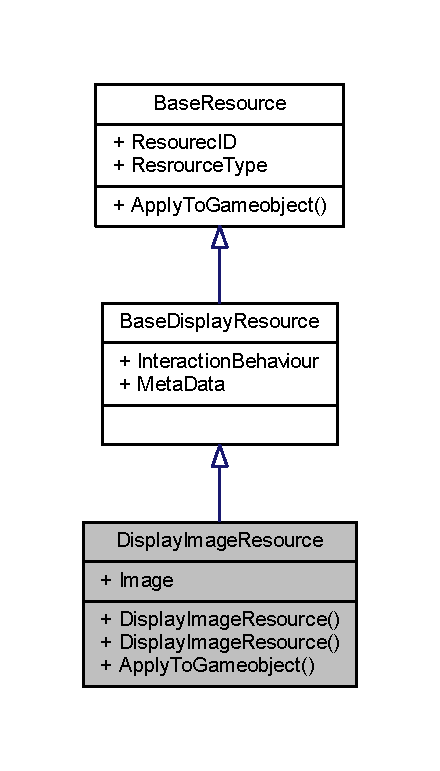
\includegraphics[width=211pt]{class_display_image_resource__inherit__graph}
\end{center}
\end{figure}


Collaboration diagram for Display\+Image\+Resource\+:
\nopagebreak
\begin{figure}[H]
\begin{center}
\leavevmode
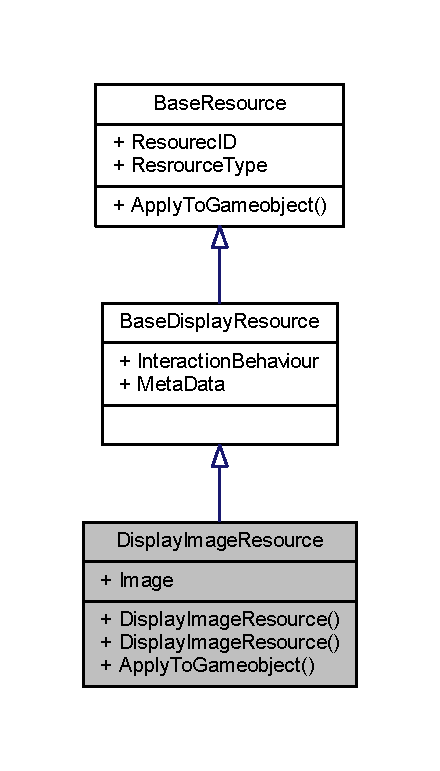
\includegraphics[width=211pt]{class_display_image_resource__coll__graph}
\end{center}
\end{figure}
\subsection*{Public Member Functions}
\begin{DoxyCompactItemize}
\item 
\mbox{\hyperlink{class_display_image_resource_a8c3e434da20e617201d74cfdb913817b}{Display\+Image\+Resource}} ()
\begin{DoxyCompactList}\small\item\em no param ctor, does not initialize anything \end{DoxyCompactList}\item 
\mbox{\hyperlink{class_display_image_resource_aa7b4bf3e8d324ea5b789322748b21b8e}{Display\+Image\+Resource}} (Texture2D img)
\begin{DoxyCompactList}\small\item\em ctor that sets the texture of the resource \end{DoxyCompactList}\item 
override void \mbox{\hyperlink{class_display_image_resource_a26992a5ecb6c449d85539cc5d07112e2}{Apply\+To\+Gameobject}} (Game\+Object obj)
\begin{DoxyCompactList}\small\item\em applies texture to gamobject by getting the meshrenderer of the object or adding one if it does not exist and setting the material of the render to a new material with the defualt sprites shader and the Image as texture \end{DoxyCompactList}\end{DoxyCompactItemize}
\subsection*{Properties}
\begin{DoxyCompactItemize}
\item 
Texture2D \mbox{\hyperlink{class_display_image_resource_a6268f6612b7c533eafc2b6c8f91c2925}{Image}}\hspace{0.3cm}{\ttfamily  \mbox{[}get, set\mbox{]}}
\end{DoxyCompactItemize}
\subsection*{Additional Inherited Members}


\subsection{Detailed Description}
resource that is a image that needs to be displayed 



\subsection{Constructor \& Destructor Documentation}
\mbox{\Hypertarget{class_display_image_resource_a8c3e434da20e617201d74cfdb913817b}\label{class_display_image_resource_a8c3e434da20e617201d74cfdb913817b}} 
\index{Display\+Image\+Resource@{Display\+Image\+Resource}!Display\+Image\+Resource@{Display\+Image\+Resource}}
\index{Display\+Image\+Resource@{Display\+Image\+Resource}!Display\+Image\+Resource@{Display\+Image\+Resource}}
\subsubsection{\texorpdfstring{Display\+Image\+Resource()}{DisplayImageResource()}\hspace{0.1cm}{\footnotesize\ttfamily [1/2]}}
{\footnotesize\ttfamily Display\+Image\+Resource.\+Display\+Image\+Resource (\begin{DoxyParamCaption}{ }\end{DoxyParamCaption})}



no param ctor, does not initialize anything 

\mbox{\Hypertarget{class_display_image_resource_aa7b4bf3e8d324ea5b789322748b21b8e}\label{class_display_image_resource_aa7b4bf3e8d324ea5b789322748b21b8e}} 
\index{Display\+Image\+Resource@{Display\+Image\+Resource}!Display\+Image\+Resource@{Display\+Image\+Resource}}
\index{Display\+Image\+Resource@{Display\+Image\+Resource}!Display\+Image\+Resource@{Display\+Image\+Resource}}
\subsubsection{\texorpdfstring{Display\+Image\+Resource()}{DisplayImageResource()}\hspace{0.1cm}{\footnotesize\ttfamily [2/2]}}
{\footnotesize\ttfamily Display\+Image\+Resource.\+Display\+Image\+Resource (\begin{DoxyParamCaption}\item[{Texture2D}]{img }\end{DoxyParamCaption})}



ctor that sets the texture of the resource 


\begin{DoxyParams}{Parameters}
{\em img} & the texture of the resource\\
\hline
\end{DoxyParams}


\subsection{Member Function Documentation}
\mbox{\Hypertarget{class_display_image_resource_a26992a5ecb6c449d85539cc5d07112e2}\label{class_display_image_resource_a26992a5ecb6c449d85539cc5d07112e2}} 
\index{Display\+Image\+Resource@{Display\+Image\+Resource}!Apply\+To\+Gameobject@{Apply\+To\+Gameobject}}
\index{Apply\+To\+Gameobject@{Apply\+To\+Gameobject}!Display\+Image\+Resource@{Display\+Image\+Resource}}
\subsubsection{\texorpdfstring{Apply\+To\+Gameobject()}{ApplyToGameobject()}}
{\footnotesize\ttfamily override void Display\+Image\+Resource.\+Apply\+To\+Gameobject (\begin{DoxyParamCaption}\item[{Game\+Object}]{obj }\end{DoxyParamCaption})\hspace{0.3cm}{\ttfamily [virtual]}}



applies texture to gamobject by getting the meshrenderer of the object or adding one if it does not exist and setting the material of the render to a new material with the defualt sprites shader and the Image as texture 


\begin{DoxyParams}{Parameters}
{\em obj} & \\
\hline
\end{DoxyParams}


Implements \mbox{\hyperlink{class_base_resource_a2d832c8042114da9e3f6240651d59703}{Base\+Resource}}.



\subsection{Property Documentation}
\mbox{\Hypertarget{class_display_image_resource_a6268f6612b7c533eafc2b6c8f91c2925}\label{class_display_image_resource_a6268f6612b7c533eafc2b6c8f91c2925}} 
\index{Display\+Image\+Resource@{Display\+Image\+Resource}!Image@{Image}}
\index{Image@{Image}!Display\+Image\+Resource@{Display\+Image\+Resource}}
\subsubsection{\texorpdfstring{Image}{Image}}
{\footnotesize\ttfamily Texture2D Display\+Image\+Resource.\+Image\hspace{0.3cm}{\ttfamily [get]}, {\ttfamily [set]}}



The documentation for this class was generated from the following file\+:\begin{DoxyCompactItemize}
\item 
C\+:/\+Unity\+Projects/\+Virt\+Muse/\+Room\+Gen\+Prototype/\+Assets/\+Scripts/\+Resources/\mbox{\hyperlink{_resource_8cs}{Resource.\+cs}}\end{DoxyCompactItemize}

\hypertarget{class_display_mesh_resource}{}\section{Display\+Mesh\+Resource Class Reference}
\label{class_display_mesh_resource}\index{Display\+Mesh\+Resource@{Display\+Mesh\+Resource}}


a resource that is a mesh  




Inheritance diagram for Display\+Mesh\+Resource\+:
\nopagebreak
\begin{figure}[H]
\begin{center}
\leavevmode
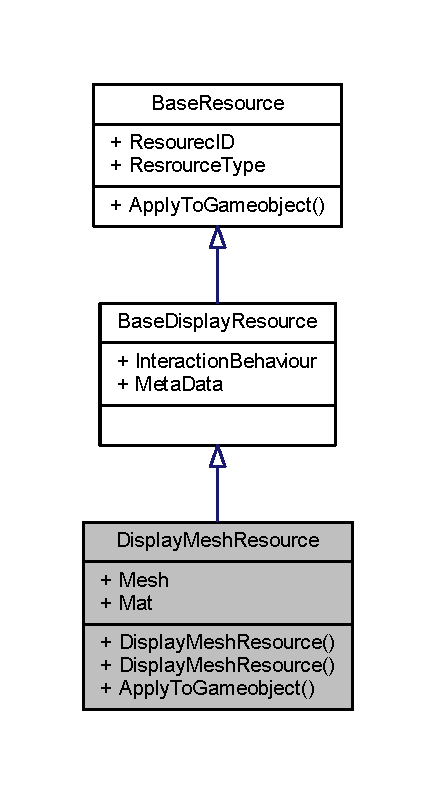
\includegraphics[width=209pt]{class_display_mesh_resource__inherit__graph}
\end{center}
\end{figure}


Collaboration diagram for Display\+Mesh\+Resource\+:
\nopagebreak
\begin{figure}[H]
\begin{center}
\leavevmode
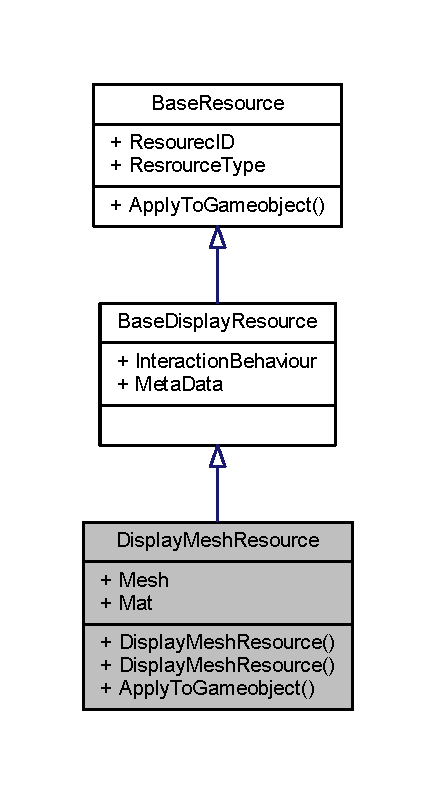
\includegraphics[width=209pt]{class_display_mesh_resource__coll__graph}
\end{center}
\end{figure}
\subsection*{Public Member Functions}
\begin{DoxyCompactItemize}
\item 
\mbox{\hyperlink{class_display_mesh_resource_ab51d570e0165de27fc603b69ae026e6b}{Display\+Mesh\+Resource}} ()
\item 
\mbox{\hyperlink{class_display_mesh_resource_aa4b6bc70724de2c056737f015cad4a41}{Display\+Mesh\+Resource}} (\mbox{\hyperlink{class_display_mesh_resource_a3ea74e82fc6354c0d84ed87b996e64d9}{Mesh}} msh, Material mat)
\item 
override void \mbox{\hyperlink{class_display_mesh_resource_a62672f28a402bebeed1cb79fcca81828}{Apply\+To\+Gameobject}} (Game\+Object obj)
\begin{DoxyCompactList}\small\item\em function that applies a resource to a gamobject \end{DoxyCompactList}\end{DoxyCompactItemize}
\subsection*{Properties}
\begin{DoxyCompactItemize}
\item 
Mesh \mbox{\hyperlink{class_display_mesh_resource_a3ea74e82fc6354c0d84ed87b996e64d9}{Mesh}}\hspace{0.3cm}{\ttfamily  \mbox{[}get, set\mbox{]}}
\item 
Material \mbox{\hyperlink{class_display_mesh_resource_addb4fd55147fa231d6ea1acc8a7a6cf5}{Mat}}\hspace{0.3cm}{\ttfamily  \mbox{[}get, set\mbox{]}}
\end{DoxyCompactItemize}
\subsection*{Additional Inherited Members}


\subsection{Detailed Description}
a resource that is a mesh 



\subsection{Constructor \& Destructor Documentation}
\mbox{\Hypertarget{class_display_mesh_resource_ab51d570e0165de27fc603b69ae026e6b}\label{class_display_mesh_resource_ab51d570e0165de27fc603b69ae026e6b}} 
\index{Display\+Mesh\+Resource@{Display\+Mesh\+Resource}!Display\+Mesh\+Resource@{Display\+Mesh\+Resource}}
\index{Display\+Mesh\+Resource@{Display\+Mesh\+Resource}!Display\+Mesh\+Resource@{Display\+Mesh\+Resource}}
\subsubsection{\texorpdfstring{Display\+Mesh\+Resource()}{DisplayMeshResource()}\hspace{0.1cm}{\footnotesize\ttfamily [1/2]}}
{\footnotesize\ttfamily Display\+Mesh\+Resource.\+Display\+Mesh\+Resource (\begin{DoxyParamCaption}{ }\end{DoxyParamCaption})}

\mbox{\Hypertarget{class_display_mesh_resource_aa4b6bc70724de2c056737f015cad4a41}\label{class_display_mesh_resource_aa4b6bc70724de2c056737f015cad4a41}} 
\index{Display\+Mesh\+Resource@{Display\+Mesh\+Resource}!Display\+Mesh\+Resource@{Display\+Mesh\+Resource}}
\index{Display\+Mesh\+Resource@{Display\+Mesh\+Resource}!Display\+Mesh\+Resource@{Display\+Mesh\+Resource}}
\subsubsection{\texorpdfstring{Display\+Mesh\+Resource()}{DisplayMeshResource()}\hspace{0.1cm}{\footnotesize\ttfamily [2/2]}}
{\footnotesize\ttfamily Display\+Mesh\+Resource.\+Display\+Mesh\+Resource (\begin{DoxyParamCaption}\item[{\mbox{\hyperlink{class_display_mesh_resource_a3ea74e82fc6354c0d84ed87b996e64d9}{Mesh}}}]{msh,  }\item[{Material}]{mat }\end{DoxyParamCaption})}



\subsection{Member Function Documentation}
\mbox{\Hypertarget{class_display_mesh_resource_a62672f28a402bebeed1cb79fcca81828}\label{class_display_mesh_resource_a62672f28a402bebeed1cb79fcca81828}} 
\index{Display\+Mesh\+Resource@{Display\+Mesh\+Resource}!Apply\+To\+Gameobject@{Apply\+To\+Gameobject}}
\index{Apply\+To\+Gameobject@{Apply\+To\+Gameobject}!Display\+Mesh\+Resource@{Display\+Mesh\+Resource}}
\subsubsection{\texorpdfstring{Apply\+To\+Gameobject()}{ApplyToGameobject()}}
{\footnotesize\ttfamily override void Display\+Mesh\+Resource.\+Apply\+To\+Gameobject (\begin{DoxyParamCaption}\item[{Game\+Object}]{obj }\end{DoxyParamCaption})\hspace{0.3cm}{\ttfamily [virtual]}}



function that applies a resource to a gamobject 


\begin{DoxyParams}{Parameters}
{\em obj} & the object the resource is applied to\\
\hline
\end{DoxyParams}


Implements \mbox{\hyperlink{class_base_resource_a2d832c8042114da9e3f6240651d59703}{Base\+Resource}}.



\subsection{Property Documentation}
\mbox{\Hypertarget{class_display_mesh_resource_addb4fd55147fa231d6ea1acc8a7a6cf5}\label{class_display_mesh_resource_addb4fd55147fa231d6ea1acc8a7a6cf5}} 
\index{Display\+Mesh\+Resource@{Display\+Mesh\+Resource}!Mat@{Mat}}
\index{Mat@{Mat}!Display\+Mesh\+Resource@{Display\+Mesh\+Resource}}
\subsubsection{\texorpdfstring{Mat}{Mat}}
{\footnotesize\ttfamily Material Display\+Mesh\+Resource.\+Mat\hspace{0.3cm}{\ttfamily [get]}, {\ttfamily [set]}}

\mbox{\Hypertarget{class_display_mesh_resource_a3ea74e82fc6354c0d84ed87b996e64d9}\label{class_display_mesh_resource_a3ea74e82fc6354c0d84ed87b996e64d9}} 
\index{Display\+Mesh\+Resource@{Display\+Mesh\+Resource}!Mesh@{Mesh}}
\index{Mesh@{Mesh}!Display\+Mesh\+Resource@{Display\+Mesh\+Resource}}
\subsubsection{\texorpdfstring{Mesh}{Mesh}}
{\footnotesize\ttfamily Mesh Display\+Mesh\+Resource.\+Mesh\hspace{0.3cm}{\ttfamily [get]}, {\ttfamily [set]}}



The documentation for this class was generated from the following file\+:\begin{DoxyCompactItemize}
\item 
C\+:/\+Unity\+Projects/\+Virt\+Muse/\+Room\+Gen\+Prototype/\+Assets/\+Scripts/\+Resources/\mbox{\hyperlink{_resource_8cs}{Resource.\+cs}}\end{DoxyCompactItemize}

\hypertarget{class_door_trigger}{}\section{Door\+Trigger Class Reference}
\label{class_door_trigger}\index{Door\+Trigger@{Door\+Trigger}}


Box collider trigger that opens and closes a door it is responsible for  




Inheritance diagram for Door\+Trigger\+:
\nopagebreak
\begin{figure}[H]
\begin{center}
\leavevmode
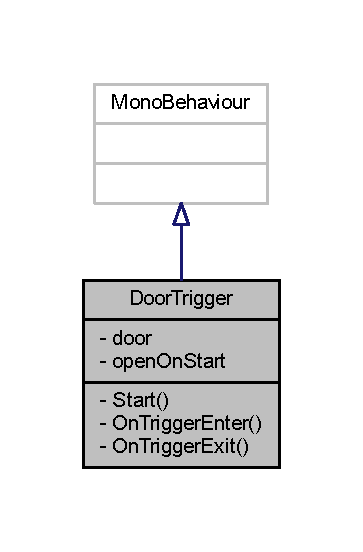
\includegraphics[width=163pt]{class_door_trigger__inherit__graph}
\end{center}
\end{figure}


Collaboration diagram for Door\+Trigger\+:
\nopagebreak
\begin{figure}[H]
\begin{center}
\leavevmode
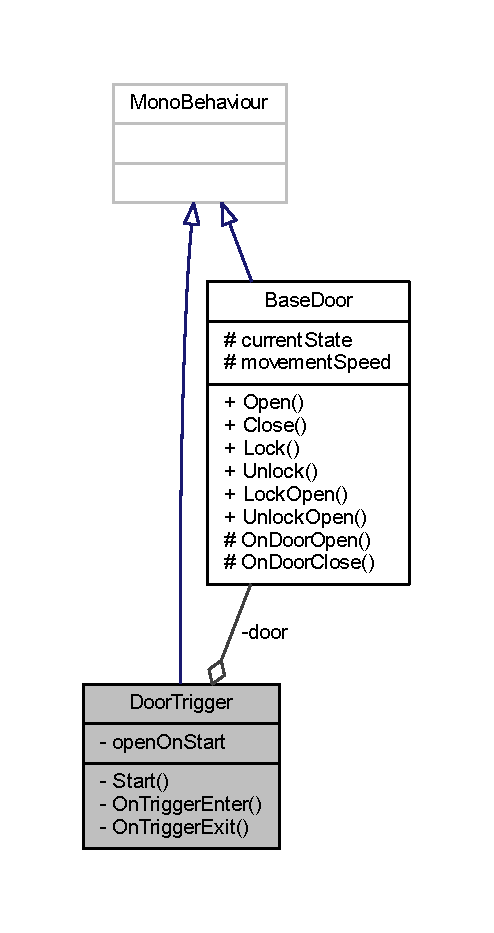
\includegraphics[width=189pt]{class_door_trigger__coll__graph}
\end{center}
\end{figure}
\subsection*{Events}
\begin{DoxyCompactItemize}
\item 
Action$<$ Collider, \mbox{\hyperlink{class_base_door}{Base\+Door}} $>$ \mbox{\hyperlink{class_door_trigger_aaf26dd7fb0f0ce643f5fd50805e2b4e0}{On\+Collider\+Enter}}
\item 
Action$<$ Collider, \mbox{\hyperlink{class_base_door}{Base\+Door}} $>$ \mbox{\hyperlink{class_door_trigger_af00f29ad47c5853b9f8ff03048223e30}{On\+Collider\+Leave}}
\end{DoxyCompactItemize}
\subsection*{Private Member Functions}
\begin{DoxyCompactItemize}
\item 
void \mbox{\hyperlink{class_door_trigger_a3b079888a26feb3139b6a0507b89c65c}{Start}} ()
\item 
void \mbox{\hyperlink{class_door_trigger_a9cad842a8527ec462aae682c8c50b118}{On\+Trigger\+Enter}} (Collider other)
\item 
void \mbox{\hyperlink{class_door_trigger_adee54426b691466c5d667b912816bb56}{On\+Trigger\+Exit}} (Collider other)
\end{DoxyCompactItemize}
\subsection*{Private Attributes}
\begin{DoxyCompactItemize}
\item 
\mbox{\hyperlink{class_base_door}{Base\+Door}} \mbox{\hyperlink{class_door_trigger_a592b30ac7c1c4b719d6a90fa96fbb046}{door}}
\item 
bool \mbox{\hyperlink{class_door_trigger_ac3f14399b44bff7efd22f9ce4d4ef5c6}{open\+On\+Start}} = true
\end{DoxyCompactItemize}


\subsection{Detailed Description}
Box collider trigger that opens and closes a door it is responsible for 



\subsection{Member Function Documentation}
\mbox{\Hypertarget{class_door_trigger_a9cad842a8527ec462aae682c8c50b118}\label{class_door_trigger_a9cad842a8527ec462aae682c8c50b118}} 
\index{Door\+Trigger@{Door\+Trigger}!On\+Trigger\+Enter@{On\+Trigger\+Enter}}
\index{On\+Trigger\+Enter@{On\+Trigger\+Enter}!Door\+Trigger@{Door\+Trigger}}
\subsubsection{\texorpdfstring{On\+Trigger\+Enter()}{OnTriggerEnter()}}
{\footnotesize\ttfamily void Door\+Trigger.\+On\+Trigger\+Enter (\begin{DoxyParamCaption}\item[{Collider}]{other }\end{DoxyParamCaption})\hspace{0.3cm}{\ttfamily [private]}}

Here is the call graph for this function\+:
\nopagebreak
\begin{figure}[H]
\begin{center}
\leavevmode
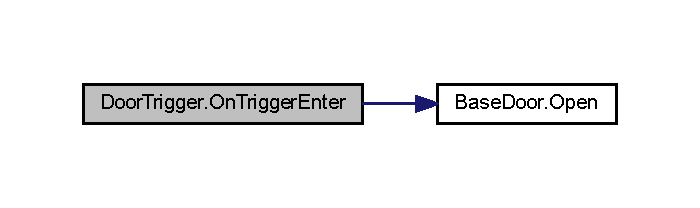
\includegraphics[width=336pt]{class_door_trigger_a9cad842a8527ec462aae682c8c50b118_cgraph}
\end{center}
\end{figure}
\mbox{\Hypertarget{class_door_trigger_adee54426b691466c5d667b912816bb56}\label{class_door_trigger_adee54426b691466c5d667b912816bb56}} 
\index{Door\+Trigger@{Door\+Trigger}!On\+Trigger\+Exit@{On\+Trigger\+Exit}}
\index{On\+Trigger\+Exit@{On\+Trigger\+Exit}!Door\+Trigger@{Door\+Trigger}}
\subsubsection{\texorpdfstring{On\+Trigger\+Exit()}{OnTriggerExit()}}
{\footnotesize\ttfamily void Door\+Trigger.\+On\+Trigger\+Exit (\begin{DoxyParamCaption}\item[{Collider}]{other }\end{DoxyParamCaption})\hspace{0.3cm}{\ttfamily [private]}}

Here is the call graph for this function\+:
\nopagebreak
\begin{figure}[H]
\begin{center}
\leavevmode
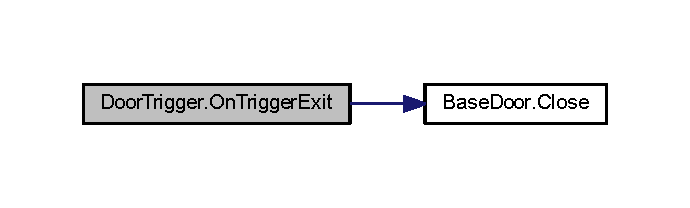
\includegraphics[width=331pt]{class_door_trigger_adee54426b691466c5d667b912816bb56_cgraph}
\end{center}
\end{figure}
\mbox{\Hypertarget{class_door_trigger_a3b079888a26feb3139b6a0507b89c65c}\label{class_door_trigger_a3b079888a26feb3139b6a0507b89c65c}} 
\index{Door\+Trigger@{Door\+Trigger}!Start@{Start}}
\index{Start@{Start}!Door\+Trigger@{Door\+Trigger}}
\subsubsection{\texorpdfstring{Start()}{Start()}}
{\footnotesize\ttfamily void Door\+Trigger.\+Start (\begin{DoxyParamCaption}{ }\end{DoxyParamCaption})\hspace{0.3cm}{\ttfamily [private]}}

Here is the call graph for this function\+:
\nopagebreak
\begin{figure}[H]
\begin{center}
\leavevmode
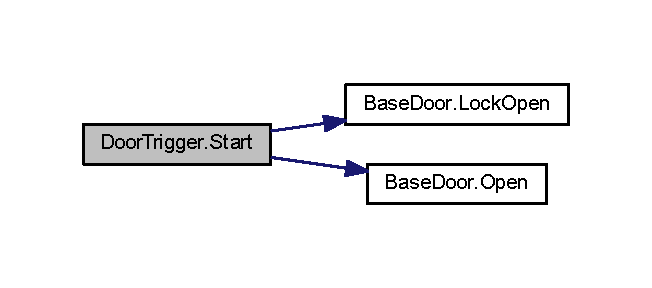
\includegraphics[width=313pt]{class_door_trigger_a3b079888a26feb3139b6a0507b89c65c_cgraph}
\end{center}
\end{figure}


\subsection{Member Data Documentation}
\mbox{\Hypertarget{class_door_trigger_a592b30ac7c1c4b719d6a90fa96fbb046}\label{class_door_trigger_a592b30ac7c1c4b719d6a90fa96fbb046}} 
\index{Door\+Trigger@{Door\+Trigger}!door@{door}}
\index{door@{door}!Door\+Trigger@{Door\+Trigger}}
\subsubsection{\texorpdfstring{door}{door}}
{\footnotesize\ttfamily \mbox{\hyperlink{class_base_door}{Base\+Door}} Door\+Trigger.\+door\hspace{0.3cm}{\ttfamily [private]}}

\mbox{\Hypertarget{class_door_trigger_ac3f14399b44bff7efd22f9ce4d4ef5c6}\label{class_door_trigger_ac3f14399b44bff7efd22f9ce4d4ef5c6}} 
\index{Door\+Trigger@{Door\+Trigger}!open\+On\+Start@{open\+On\+Start}}
\index{open\+On\+Start@{open\+On\+Start}!Door\+Trigger@{Door\+Trigger}}
\subsubsection{\texorpdfstring{open\+On\+Start}{openOnStart}}
{\footnotesize\ttfamily bool Door\+Trigger.\+open\+On\+Start = true\hspace{0.3cm}{\ttfamily [private]}}



\subsection{Event Documentation}
\mbox{\Hypertarget{class_door_trigger_aaf26dd7fb0f0ce643f5fd50805e2b4e0}\label{class_door_trigger_aaf26dd7fb0f0ce643f5fd50805e2b4e0}} 
\index{Door\+Trigger@{Door\+Trigger}!On\+Collider\+Enter@{On\+Collider\+Enter}}
\index{On\+Collider\+Enter@{On\+Collider\+Enter}!Door\+Trigger@{Door\+Trigger}}
\subsubsection{\texorpdfstring{On\+Collider\+Enter}{OnColliderEnter}}
{\footnotesize\ttfamily Action$<$Collider, \mbox{\hyperlink{class_base_door}{Base\+Door}}$>$ Door\+Trigger.\+On\+Collider\+Enter}

\mbox{\Hypertarget{class_door_trigger_af00f29ad47c5853b9f8ff03048223e30}\label{class_door_trigger_af00f29ad47c5853b9f8ff03048223e30}} 
\index{Door\+Trigger@{Door\+Trigger}!On\+Collider\+Leave@{On\+Collider\+Leave}}
\index{On\+Collider\+Leave@{On\+Collider\+Leave}!Door\+Trigger@{Door\+Trigger}}
\subsubsection{\texorpdfstring{On\+Collider\+Leave}{OnColliderLeave}}
{\footnotesize\ttfamily Action$<$Collider, \mbox{\hyperlink{class_base_door}{Base\+Door}}$>$ Door\+Trigger.\+On\+Collider\+Leave}



The documentation for this class was generated from the following file\+:\begin{DoxyCompactItemize}
\item 
C\+:/\+Unity\+Projects/\+Virt\+Muse/\+Room\+Gen\+Prototype/\+Assets/\+Scripts/\+Door/\mbox{\hyperlink{_door_trigger_8cs}{Door\+Trigger.\+cs}}\end{DoxyCompactItemize}

\hypertarget{interface_i_holdable_object}{}\section{I\+Holdable\+Object Interface Reference}
\label{interface_i_holdable_object}\index{I\+Holdable\+Object@{I\+Holdable\+Object}}


Inheritance diagram for I\+Holdable\+Object\+:
\nopagebreak
\begin{figure}[H]
\begin{center}
\leavevmode
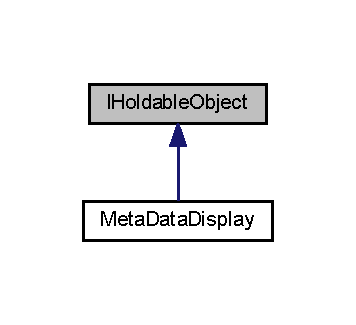
\includegraphics[width=171pt]{interface_i_holdable_object__inherit__graph}
\end{center}
\end{figure}
\subsection*{Public Member Functions}
\begin{DoxyCompactItemize}
\item 
void \mbox{\hyperlink{interface_i_holdable_object_a6f63fec8fb8f715ad5cdd08aa5ec0ea5}{On\+Held\+Infront\+Of\+Face}} ()
\begin{DoxyCompactList}\small\item\em called when hand reaches infront of face position right after state was set to infront of face \end{DoxyCompactList}\item 
void \mbox{\hyperlink{interface_i_holdable_object_abe7c5e5ed97fb5c908c91da5b8714f0e}{On\+Put\+Away}} ()
\begin{DoxyCompactList}\small\item\em Called when the hand reaches it\textquotesingle{}s rest positon right after the state is set to Rest\+Position \end{DoxyCompactList}\item 
void \mbox{\hyperlink{interface_i_holdable_object_af5dcdd5524539104706dadd8a0e15e08}{On\+Started\+Move\+Infront\+Of\+Face}} ()
\begin{DoxyCompactList}\small\item\em called when hand starts moving towards the infront of face position right after the state is set to Moving\+Infrontof\+Face \end{DoxyCompactList}\item 
void \mbox{\hyperlink{interface_i_holdable_object_a75f802a9736db51e5e8d1568689dd11c}{On\+Started\+Move\+Away\+From\+Face}} ()
\begin{DoxyCompactList}\small\item\em called when the hand starts moving away from the face right after the hand state is set to Moving\+To\+Rest\+Position \end{DoxyCompactList}\item 
void \mbox{\hyperlink{interface_i_holdable_object_a3fe2e7a7d0740225142053583f438333}{Position\+Object\+In\+Hand}} (\mbox{\hyperlink{class_player_hand}{Player\+Hand}} hand)
\begin{DoxyCompactList}\small\item\em used to probably parent obj to hand gamobjt and set local position called by grab object of the hand \end{DoxyCompactList}\item 
void \mbox{\hyperlink{interface_i_holdable_object_a7b8a42a0c12a26b1668c4dd904f38355}{On\+Grabed}} (\mbox{\hyperlink{class_player_hand}{Player\+Hand}} hand)
\begin{DoxyCompactList}\small\item\em Called the frame this object is grabbed can be seen as an initializer function for when the obj is grabbed \end{DoxyCompactList}\item 
void \mbox{\hyperlink{interface_i_holdable_object_a19523673c41505d8533aa50b957e95a1}{On\+Dropped}} (\mbox{\hyperlink{class_player_hand}{Player\+Hand}} hand)
\begin{DoxyCompactList}\small\item\em Called the frame this object is dropped by a hand can be seen as a destroy/cleanup function for the opbject when called the hand does not hold the object anyomre \end{DoxyCompactList}\item 
bool \mbox{\hyperlink{interface_i_holdable_object_a0356d534c17ab4e04fba00b42abeea77}{Is\+Interested\+In\+Interactable\+Objects}} ()
\begin{DoxyCompactList}\small\item\em this functions defines iof the held object gets information about an interactable object forwarded to him \end{DoxyCompactList}\item 
void \mbox{\hyperlink{interface_i_holdable_object_aeb32a55273b99d16f9fb5b86f6a73f80}{Set\+Interacted\+Object}} (\mbox{\hyperlink{interface_i_interactable}{I\+Interactable}} i\+Obj)
\begin{DoxyCompactList}\small\item\em function get\textquotesingle{}s called by hand if the held object is interessted in interacted objects \end{DoxyCompactList}\end{DoxyCompactItemize}
\subsection*{Properties}
\begin{DoxyCompactItemize}
\item 
Game\+Object \mbox{\hyperlink{interface_i_holdable_object_a99b6760e4f5c71c79d8b084673a3818b}{Object}}\hspace{0.3cm}{\ttfamily  \mbox{[}get\mbox{]}}
\begin{DoxyCompactList}\small\item\em the gameobject this interface(actually mono behav implementign it but don\textquotesingle{}t sweat it) is attached to \end{DoxyCompactList}\end{DoxyCompactItemize}


\subsection{Member Function Documentation}
\mbox{\Hypertarget{interface_i_holdable_object_a0356d534c17ab4e04fba00b42abeea77}\label{interface_i_holdable_object_a0356d534c17ab4e04fba00b42abeea77}} 
\index{I\+Holdable\+Object@{I\+Holdable\+Object}!Is\+Interested\+In\+Interactable\+Objects@{Is\+Interested\+In\+Interactable\+Objects}}
\index{Is\+Interested\+In\+Interactable\+Objects@{Is\+Interested\+In\+Interactable\+Objects}!I\+Holdable\+Object@{I\+Holdable\+Object}}
\subsubsection{\texorpdfstring{Is\+Interested\+In\+Interactable\+Objects()}{IsInterestedInInteractableObjects()}}
{\footnotesize\ttfamily bool I\+Holdable\+Object.\+Is\+Interested\+In\+Interactable\+Objects (\begin{DoxyParamCaption}{ }\end{DoxyParamCaption})}



this functions defines iof the held object gets information about an interactable object forwarded to him 

\begin{DoxyReturn}{Returns}

\end{DoxyReturn}


Implemented in \mbox{\hyperlink{class_meta_data_display_a6aa943864ef85667977a13c895c2ce23}{Meta\+Data\+Display}}.

Here is the caller graph for this function\+:
\nopagebreak
\begin{figure}[H]
\begin{center}
\leavevmode
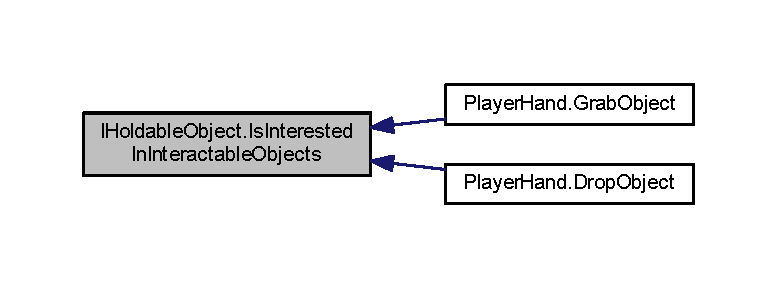
\includegraphics[width=350pt]{interface_i_holdable_object_a0356d534c17ab4e04fba00b42abeea77_icgraph}
\end{center}
\end{figure}
\mbox{\Hypertarget{interface_i_holdable_object_a19523673c41505d8533aa50b957e95a1}\label{interface_i_holdable_object_a19523673c41505d8533aa50b957e95a1}} 
\index{I\+Holdable\+Object@{I\+Holdable\+Object}!On\+Dropped@{On\+Dropped}}
\index{On\+Dropped@{On\+Dropped}!I\+Holdable\+Object@{I\+Holdable\+Object}}
\subsubsection{\texorpdfstring{On\+Dropped()}{OnDropped()}}
{\footnotesize\ttfamily void I\+Holdable\+Object.\+On\+Dropped (\begin{DoxyParamCaption}\item[{\mbox{\hyperlink{class_player_hand}{Player\+Hand}}}]{hand }\end{DoxyParamCaption})}



Called the frame this object is dropped by a hand can be seen as a destroy/cleanup function for the opbject when called the hand does not hold the object anyomre 


\begin{DoxyParams}{Parameters}
{\em hand} & the hand that held the object\\
\hline
\end{DoxyParams}


Implemented in \mbox{\hyperlink{class_meta_data_display_a274478924e6a4df19484a469ae2869ce}{Meta\+Data\+Display}}.

Here is the caller graph for this function\+:
\nopagebreak
\begin{figure}[H]
\begin{center}
\leavevmode
\includegraphics[width=350pt]{interface_i_holdable_object_a19523673c41505d8533aa50b957e95a1_icgraph}
\end{center}
\end{figure}
\mbox{\Hypertarget{interface_i_holdable_object_a7b8a42a0c12a26b1668c4dd904f38355}\label{interface_i_holdable_object_a7b8a42a0c12a26b1668c4dd904f38355}} 
\index{I\+Holdable\+Object@{I\+Holdable\+Object}!On\+Grabed@{On\+Grabed}}
\index{On\+Grabed@{On\+Grabed}!I\+Holdable\+Object@{I\+Holdable\+Object}}
\subsubsection{\texorpdfstring{On\+Grabed()}{OnGrabed()}}
{\footnotesize\ttfamily void I\+Holdable\+Object.\+On\+Grabed (\begin{DoxyParamCaption}\item[{\mbox{\hyperlink{class_player_hand}{Player\+Hand}}}]{hand }\end{DoxyParamCaption})}



Called the frame this object is grabbed can be seen as an initializer function for when the obj is grabbed 


\begin{DoxyParams}{Parameters}
{\em hand} & the hand that grabed this object\\
\hline
\end{DoxyParams}


Implemented in \mbox{\hyperlink{class_meta_data_display_a7d639d7bc58c9340a7f5274884bbc11d}{Meta\+Data\+Display}}.

Here is the caller graph for this function\+:
\nopagebreak
\begin{figure}[H]
\begin{center}
\leavevmode
\includegraphics[width=350pt]{interface_i_holdable_object_a7b8a42a0c12a26b1668c4dd904f38355_icgraph}
\end{center}
\end{figure}
\mbox{\Hypertarget{interface_i_holdable_object_a6f63fec8fb8f715ad5cdd08aa5ec0ea5}\label{interface_i_holdable_object_a6f63fec8fb8f715ad5cdd08aa5ec0ea5}} 
\index{I\+Holdable\+Object@{I\+Holdable\+Object}!On\+Held\+Infront\+Of\+Face@{On\+Held\+Infront\+Of\+Face}}
\index{On\+Held\+Infront\+Of\+Face@{On\+Held\+Infront\+Of\+Face}!I\+Holdable\+Object@{I\+Holdable\+Object}}
\subsubsection{\texorpdfstring{On\+Held\+Infront\+Of\+Face()}{OnHeldInfrontOfFace()}}
{\footnotesize\ttfamily void I\+Holdable\+Object.\+On\+Held\+Infront\+Of\+Face (\begin{DoxyParamCaption}{ }\end{DoxyParamCaption})}



called when hand reaches infront of face position right after state was set to infront of face 



Implemented in \mbox{\hyperlink{class_meta_data_display_ab91c62e23ca6af27f8a30859d5a172c9}{Meta\+Data\+Display}}.

Here is the caller graph for this function\+:
\nopagebreak
\begin{figure}[H]
\begin{center}
\leavevmode
\includegraphics[width=350pt]{interface_i_holdable_object_a6f63fec8fb8f715ad5cdd08aa5ec0ea5_icgraph}
\end{center}
\end{figure}
\mbox{\Hypertarget{interface_i_holdable_object_abe7c5e5ed97fb5c908c91da5b8714f0e}\label{interface_i_holdable_object_abe7c5e5ed97fb5c908c91da5b8714f0e}} 
\index{I\+Holdable\+Object@{I\+Holdable\+Object}!On\+Put\+Away@{On\+Put\+Away}}
\index{On\+Put\+Away@{On\+Put\+Away}!I\+Holdable\+Object@{I\+Holdable\+Object}}
\subsubsection{\texorpdfstring{On\+Put\+Away()}{OnPutAway()}}
{\footnotesize\ttfamily void I\+Holdable\+Object.\+On\+Put\+Away (\begin{DoxyParamCaption}{ }\end{DoxyParamCaption})}



Called when the hand reaches it\textquotesingle{}s rest positon right after the state is set to Rest\+Position 



Implemented in \mbox{\hyperlink{class_meta_data_display_a55888c6c3e3e224d89d95b6c63652762}{Meta\+Data\+Display}}.

Here is the caller graph for this function\+:
\nopagebreak
\begin{figure}[H]
\begin{center}
\leavevmode
\includegraphics[width=350pt]{interface_i_holdable_object_abe7c5e5ed97fb5c908c91da5b8714f0e_icgraph}
\end{center}
\end{figure}
\mbox{\Hypertarget{interface_i_holdable_object_a75f802a9736db51e5e8d1568689dd11c}\label{interface_i_holdable_object_a75f802a9736db51e5e8d1568689dd11c}} 
\index{I\+Holdable\+Object@{I\+Holdable\+Object}!On\+Started\+Move\+Away\+From\+Face@{On\+Started\+Move\+Away\+From\+Face}}
\index{On\+Started\+Move\+Away\+From\+Face@{On\+Started\+Move\+Away\+From\+Face}!I\+Holdable\+Object@{I\+Holdable\+Object}}
\subsubsection{\texorpdfstring{On\+Started\+Move\+Away\+From\+Face()}{OnStartedMoveAwayFromFace()}}
{\footnotesize\ttfamily void I\+Holdable\+Object.\+On\+Started\+Move\+Away\+From\+Face (\begin{DoxyParamCaption}{ }\end{DoxyParamCaption})}



called when the hand starts moving away from the face right after the hand state is set to Moving\+To\+Rest\+Position 



Implemented in \mbox{\hyperlink{class_meta_data_display_a98518b3d82ffd1e428cab9a2328fb018}{Meta\+Data\+Display}}.

Here is the caller graph for this function\+:
\nopagebreak
\begin{figure}[H]
\begin{center}
\leavevmode
\includegraphics[width=350pt]{interface_i_holdable_object_a75f802a9736db51e5e8d1568689dd11c_icgraph}
\end{center}
\end{figure}
\mbox{\Hypertarget{interface_i_holdable_object_af5dcdd5524539104706dadd8a0e15e08}\label{interface_i_holdable_object_af5dcdd5524539104706dadd8a0e15e08}} 
\index{I\+Holdable\+Object@{I\+Holdable\+Object}!On\+Started\+Move\+Infront\+Of\+Face@{On\+Started\+Move\+Infront\+Of\+Face}}
\index{On\+Started\+Move\+Infront\+Of\+Face@{On\+Started\+Move\+Infront\+Of\+Face}!I\+Holdable\+Object@{I\+Holdable\+Object}}
\subsubsection{\texorpdfstring{On\+Started\+Move\+Infront\+Of\+Face()}{OnStartedMoveInfrontOfFace()}}
{\footnotesize\ttfamily void I\+Holdable\+Object.\+On\+Started\+Move\+Infront\+Of\+Face (\begin{DoxyParamCaption}{ }\end{DoxyParamCaption})}



called when hand starts moving towards the infront of face position right after the state is set to Moving\+Infrontof\+Face 



Implemented in \mbox{\hyperlink{class_meta_data_display_aa0a9b9ca8243943104c82602e69a0541}{Meta\+Data\+Display}}.

Here is the caller graph for this function\+:
\nopagebreak
\begin{figure}[H]
\begin{center}
\leavevmode
\includegraphics[width=350pt]{interface_i_holdable_object_af5dcdd5524539104706dadd8a0e15e08_icgraph}
\end{center}
\end{figure}
\mbox{\Hypertarget{interface_i_holdable_object_a3fe2e7a7d0740225142053583f438333}\label{interface_i_holdable_object_a3fe2e7a7d0740225142053583f438333}} 
\index{I\+Holdable\+Object@{I\+Holdable\+Object}!Position\+Object\+In\+Hand@{Position\+Object\+In\+Hand}}
\index{Position\+Object\+In\+Hand@{Position\+Object\+In\+Hand}!I\+Holdable\+Object@{I\+Holdable\+Object}}
\subsubsection{\texorpdfstring{Position\+Object\+In\+Hand()}{PositionObjectInHand()}}
{\footnotesize\ttfamily void I\+Holdable\+Object.\+Position\+Object\+In\+Hand (\begin{DoxyParamCaption}\item[{\mbox{\hyperlink{class_player_hand}{Player\+Hand}}}]{hand }\end{DoxyParamCaption})}



used to probably parent obj to hand gamobjt and set local position called by grab object of the hand 


\begin{DoxyParams}{Parameters}
{\em hand} & \\
\hline
\end{DoxyParams}


Implemented in \mbox{\hyperlink{class_meta_data_display_a1ecbc336a25464fc9999120066263e2a}{Meta\+Data\+Display}}.

\mbox{\Hypertarget{interface_i_holdable_object_aeb32a55273b99d16f9fb5b86f6a73f80}\label{interface_i_holdable_object_aeb32a55273b99d16f9fb5b86f6a73f80}} 
\index{I\+Holdable\+Object@{I\+Holdable\+Object}!Set\+Interacted\+Object@{Set\+Interacted\+Object}}
\index{Set\+Interacted\+Object@{Set\+Interacted\+Object}!I\+Holdable\+Object@{I\+Holdable\+Object}}
\subsubsection{\texorpdfstring{Set\+Interacted\+Object()}{SetInteractedObject()}}
{\footnotesize\ttfamily void I\+Holdable\+Object.\+Set\+Interacted\+Object (\begin{DoxyParamCaption}\item[{\mbox{\hyperlink{interface_i_interactable}{I\+Interactable}}}]{i\+Obj }\end{DoxyParamCaption})}



function get\textquotesingle{}s called by hand if the held object is interessted in interacted objects 


\begin{DoxyParams}{Parameters}
{\em i\+Obj} & the object the player interacted with\\
\hline
\end{DoxyParams}


Implemented in \mbox{\hyperlink{class_meta_data_display_a29b7b1ec6193b73606dc7da89c387529}{Meta\+Data\+Display}}.

Here is the caller graph for this function\+:
\nopagebreak
\begin{figure}[H]
\begin{center}
\leavevmode
\includegraphics[width=350pt]{interface_i_holdable_object_aeb32a55273b99d16f9fb5b86f6a73f80_icgraph}
\end{center}
\end{figure}


\subsection{Property Documentation}
\mbox{\Hypertarget{interface_i_holdable_object_a99b6760e4f5c71c79d8b084673a3818b}\label{interface_i_holdable_object_a99b6760e4f5c71c79d8b084673a3818b}} 
\index{I\+Holdable\+Object@{I\+Holdable\+Object}!Object@{Object}}
\index{Object@{Object}!I\+Holdable\+Object@{I\+Holdable\+Object}}
\subsubsection{\texorpdfstring{Object}{Object}}
{\footnotesize\ttfamily Game\+Object I\+Holdable\+Object.\+Object\hspace{0.3cm}{\ttfamily [get]}}



the gameobject this interface(actually mono behav implementign it but don\textquotesingle{}t sweat it) is attached to 



The documentation for this interface was generated from the following file\+:\begin{DoxyCompactItemize}
\item 
C\+:/\+Unity\+Projects/\+Virt\+Muse/\+Room\+Gen\+Prototype/\+Assets/\+Scripts/\+Utility/\+Interfaces/\mbox{\hyperlink{_i_holdable_object_8cs}{I\+Holdable\+Object.\+cs}}\end{DoxyCompactItemize}

\hypertarget{interface_i_interactable}{}\section{I\+Interactable Interface Reference}
\label{interface_i_interactable}\index{I\+Interactable@{I\+Interactable}}


Inheritance diagram for I\+Interactable\+:
\nopagebreak
\begin{figure}[H]
\begin{center}
\leavevmode
\includegraphics[width=350pt]{interface_i_interactable__inherit__graph}
\end{center}
\end{figure}
\subsection*{Public Member Functions}
\begin{DoxyCompactItemize}
\item 
void \mbox{\hyperlink{interface_i_interactable_a736e28381ac0e7ca60f5fae2feb95afe}{Interact}} (\mbox{\hyperlink{class_player}{Player}} player)
\begin{DoxyCompactList}\small\item\em function called when an interaction is started by a player \end{DoxyCompactList}\end{DoxyCompactItemize}
\subsection*{Properties}
\begin{DoxyCompactItemize}
\item 
Game\+Object \mbox{\hyperlink{interface_i_interactable_a1ea155218acad8d933577fa071de48af}{Object}}\hspace{0.3cm}{\ttfamily  \mbox{[}get\mbox{]}}
\end{DoxyCompactItemize}


\subsection{Member Function Documentation}
\mbox{\Hypertarget{interface_i_interactable_a736e28381ac0e7ca60f5fae2feb95afe}\label{interface_i_interactable_a736e28381ac0e7ca60f5fae2feb95afe}} 
\index{I\+Interactable@{I\+Interactable}!Interact@{Interact}}
\index{Interact@{Interact}!I\+Interactable@{I\+Interactable}}
\subsubsection{\texorpdfstring{Interact()}{Interact()}}
{\footnotesize\ttfamily void I\+Interactable.\+Interact (\begin{DoxyParamCaption}\item[{\mbox{\hyperlink{class_player}{Player}}}]{player }\end{DoxyParamCaption})}



function called when an interaction is started by a player 


\begin{DoxyParams}{Parameters}
{\em player} & \\
\hline
\end{DoxyParams}


Implemented in \mbox{\hyperlink{class_display_a43fc2a6f19bbf2f1bdb676392b37e921}{Display}}.

Here is the caller graph for this function\+:
\nopagebreak
\begin{figure}[H]
\begin{center}
\leavevmode
\includegraphics[width=350pt]{interface_i_interactable_a736e28381ac0e7ca60f5fae2feb95afe_icgraph}
\end{center}
\end{figure}


\subsection{Property Documentation}
\mbox{\Hypertarget{interface_i_interactable_a1ea155218acad8d933577fa071de48af}\label{interface_i_interactable_a1ea155218acad8d933577fa071de48af}} 
\index{I\+Interactable@{I\+Interactable}!Object@{Object}}
\index{Object@{Object}!I\+Interactable@{I\+Interactable}}
\subsubsection{\texorpdfstring{Object}{Object}}
{\footnotesize\ttfamily Game\+Object I\+Interactable.\+Object\hspace{0.3cm}{\ttfamily [get]}}



The documentation for this interface was generated from the following file\+:\begin{DoxyCompactItemize}
\item 
C\+:/\+Unity\+Projects/\+Virt\+Muse/\+Room\+Gen\+Prototype/\+Assets/\+Scripts/\+Utility/\+Interfaces/\mbox{\hyperlink{_i_interactable_8cs}{I\+Interactable.\+cs}}\end{DoxyCompactItemize}

\hypertarget{class_image_display}{}\section{Image\+Display Class Reference}
\label{class_image_display}\index{Image\+Display@{Image\+Display}}


Inheritance diagram for Image\+Display\+:
\nopagebreak
\begin{figure}[H]
\begin{center}
\leavevmode
\includegraphics[width=250pt]{class_image_display__inherit__graph}
\end{center}
\end{figure}


Collaboration diagram for Image\+Display\+:
\nopagebreak
\begin{figure}[H]
\begin{center}
\leavevmode
\includegraphics[width=344pt]{class_image_display__coll__graph}
\end{center}
\end{figure}
\subsection*{Public Member Functions}
\begin{DoxyCompactItemize}
\item 
override void \mbox{\hyperlink{class_image_display_ab4cae8c66db7e7d77ab117fe24e63980}{Apply\+Resource}} (\mbox{\hyperlink{class_base_display_resource}{Base\+Display\+Resource}} resource)
\begin{DoxyCompactList}\small\item\em Applies a resource to a display \end{DoxyCompactList}\item 
override void \mbox{\hyperlink{class_image_display_a28fead7caeeb12490d26fae943da6a1e}{Set\+Up}} (\mbox{\hyperlink{class_museum_display_info}{Museum\+Display\+Info}} disp\+Info, Game\+Object parent)
\begin{DoxyCompactList}\small\item\em Set up the display in the museum, position and rotation \end{DoxyCompactList}\item 
override void \mbox{\hyperlink{class_image_display_a0ad82d85f6c4ec5eabb65afa1ae72bc1}{Apply\+Pre\+Processing\+Information}} (\mbox{\hyperlink{class_pre_processing_game_object_information}{Pre\+Processing\+Game\+Object\+Information}} info)
\end{DoxyCompactItemize}
\subsection*{Static Public Attributes}
\begin{DoxyCompactItemize}
\item 
static float \mbox{\hyperlink{class_image_display_ae1044419b2f9dfa64d75329e48e312de}{X\+Pos\+Scale}} = .\+55f
\begin{DoxyCompactList}\small\item\em scales the x pos when setuping \end{DoxyCompactList}\item 
static Vector3 \mbox{\hyperlink{class_image_display_a8ecd7f162065170c3f5cbcf906b11873}{Rotation}} = new Vector3(0, -\/90f, 0)
\begin{DoxyCompactList}\small\item\em the rotation of the image display \end{DoxyCompactList}\item 
static float \mbox{\hyperlink{class_image_display_aac7ba9a36c272ad5c6873119b521ed5e}{Scale}} = 0.\+2f
\begin{DoxyCompactList}\small\item\em scale of the image \end{DoxyCompactList}\item 
static float \mbox{\hyperlink{class_image_display_ac0ef458ef2e417549068a631e35f39d6}{Y\+Pos}} = -\/.\+3f
\begin{DoxyCompactList}\small\item\em local y position of the image \end{DoxyCompactList}\end{DoxyCompactItemize}
\subsection*{Protected Member Functions}
\begin{DoxyCompactItemize}
\item 
override System.\+Type \mbox{\hyperlink{class_image_display_ae975595939d76dd1db32e6f029f53ab6}{Set\+To\+Default\+Interaction\+Behaviour}} ()
\begin{DoxyCompactList}\small\item\em if the wanted behaviour is not possible or not exitent the behaviour will be set to this default \end{DoxyCompactList}\item 
override void \mbox{\hyperlink{class_image_display_a1fdf91b09cd5329059d38033f1330ffb}{Interaction\+Started}} ()
\begin{DoxyCompactList}\small\item\em called when interaction with this display started used to maybe disable anything on the display gamobject if needed \end{DoxyCompactList}\item 
override void \mbox{\hyperlink{class_image_display_a94c5928ef81449c37740d0bd0a8f4062}{Interaction\+Ended}} ()
\begin{DoxyCompactList}\small\item\em called when an interaction ends used to reactivate any component deactivated during the interaction \end{DoxyCompactList}\end{DoxyCompactItemize}
\subsection*{Private Member Functions}
\begin{DoxyCompactItemize}
\item 
void \mbox{\hyperlink{class_image_display_a3dfa32d33641e56a6623265150b8ddba}{Awake}} ()
\end{DoxyCompactItemize}
\subsection*{Private Attributes}
\begin{DoxyCompactItemize}
\item 
Raw\+Image \mbox{[}$\,$\mbox{]} \mbox{\hyperlink{class_image_display_a3f64480a2ecdc17ac43e0db335ca8a4c}{image\+Displays}}
\begin{DoxyCompactList}\small\item\em the mseh render that displays the image \end{DoxyCompactList}\end{DoxyCompactItemize}
\subsection*{Additional Inherited Members}


\subsection{Member Function Documentation}
\mbox{\Hypertarget{class_image_display_a0ad82d85f6c4ec5eabb65afa1ae72bc1}\label{class_image_display_a0ad82d85f6c4ec5eabb65afa1ae72bc1}} 
\index{Image\+Display@{Image\+Display}!Apply\+Pre\+Processing\+Information@{Apply\+Pre\+Processing\+Information}}
\index{Apply\+Pre\+Processing\+Information@{Apply\+Pre\+Processing\+Information}!Image\+Display@{Image\+Display}}
\subsubsection{\texorpdfstring{Apply\+Pre\+Processing\+Information()}{ApplyPreProcessingInformation()}}
{\footnotesize\ttfamily override void Image\+Display.\+Apply\+Pre\+Processing\+Information (\begin{DoxyParamCaption}\item[{\mbox{\hyperlink{class_pre_processing_game_object_information}{Pre\+Processing\+Game\+Object\+Information}}}]{info }\end{DoxyParamCaption})\hspace{0.3cm}{\ttfamily [virtual]}}



Implements \mbox{\hyperlink{class_display_ab9cd24c11c43dd87bc50e85a8e9e4c31}{Display}}.

\mbox{\Hypertarget{class_image_display_ab4cae8c66db7e7d77ab117fe24e63980}\label{class_image_display_ab4cae8c66db7e7d77ab117fe24e63980}} 
\index{Image\+Display@{Image\+Display}!Apply\+Resource@{Apply\+Resource}}
\index{Apply\+Resource@{Apply\+Resource}!Image\+Display@{Image\+Display}}
\subsubsection{\texorpdfstring{Apply\+Resource()}{ApplyResource()}}
{\footnotesize\ttfamily override void Image\+Display.\+Apply\+Resource (\begin{DoxyParamCaption}\item[{\mbox{\hyperlink{class_base_display_resource}{Base\+Display\+Resource}}}]{resource }\end{DoxyParamCaption})\hspace{0.3cm}{\ttfamily [virtual]}}



Applies a resource to a display 


\begin{DoxyParams}{Parameters}
{\em obj} & \\
\hline
\end{DoxyParams}


Reimplemented from \mbox{\hyperlink{class_display_a811157ddb42ae4d72f690457a08711d3}{Display}}.

\mbox{\Hypertarget{class_image_display_a3dfa32d33641e56a6623265150b8ddba}\label{class_image_display_a3dfa32d33641e56a6623265150b8ddba}} 
\index{Image\+Display@{Image\+Display}!Awake@{Awake}}
\index{Awake@{Awake}!Image\+Display@{Image\+Display}}
\subsubsection{\texorpdfstring{Awake()}{Awake()}}
{\footnotesize\ttfamily void Image\+Display.\+Awake (\begin{DoxyParamCaption}{ }\end{DoxyParamCaption})\hspace{0.3cm}{\ttfamily [private]}}

\mbox{\Hypertarget{class_image_display_a94c5928ef81449c37740d0bd0a8f4062}\label{class_image_display_a94c5928ef81449c37740d0bd0a8f4062}} 
\index{Image\+Display@{Image\+Display}!Interaction\+Ended@{Interaction\+Ended}}
\index{Interaction\+Ended@{Interaction\+Ended}!Image\+Display@{Image\+Display}}
\subsubsection{\texorpdfstring{Interaction\+Ended()}{InteractionEnded()}}
{\footnotesize\ttfamily override void Image\+Display.\+Interaction\+Ended (\begin{DoxyParamCaption}{ }\end{DoxyParamCaption})\hspace{0.3cm}{\ttfamily [protected]}, {\ttfamily [virtual]}}



called when an interaction ends used to reactivate any component deactivated during the interaction 



Implements \mbox{\hyperlink{class_display_a6fd38485267e1b78f1d1dfb589ec4ae0}{Display}}.

\mbox{\Hypertarget{class_image_display_a1fdf91b09cd5329059d38033f1330ffb}\label{class_image_display_a1fdf91b09cd5329059d38033f1330ffb}} 
\index{Image\+Display@{Image\+Display}!Interaction\+Started@{Interaction\+Started}}
\index{Interaction\+Started@{Interaction\+Started}!Image\+Display@{Image\+Display}}
\subsubsection{\texorpdfstring{Interaction\+Started()}{InteractionStarted()}}
{\footnotesize\ttfamily override void Image\+Display.\+Interaction\+Started (\begin{DoxyParamCaption}{ }\end{DoxyParamCaption})\hspace{0.3cm}{\ttfamily [protected]}, {\ttfamily [virtual]}}



called when interaction with this display started used to maybe disable anything on the display gamobject if needed 



Implements \mbox{\hyperlink{class_display_a21c51fcf185403197a78a5acfd2065de}{Display}}.

\mbox{\Hypertarget{class_image_display_ae975595939d76dd1db32e6f029f53ab6}\label{class_image_display_ae975595939d76dd1db32e6f029f53ab6}} 
\index{Image\+Display@{Image\+Display}!Set\+To\+Default\+Interaction\+Behaviour@{Set\+To\+Default\+Interaction\+Behaviour}}
\index{Set\+To\+Default\+Interaction\+Behaviour@{Set\+To\+Default\+Interaction\+Behaviour}!Image\+Display@{Image\+Display}}
\subsubsection{\texorpdfstring{Set\+To\+Default\+Interaction\+Behaviour()}{SetToDefaultInteractionBehaviour()}}
{\footnotesize\ttfamily override System.\+Type Image\+Display.\+Set\+To\+Default\+Interaction\+Behaviour (\begin{DoxyParamCaption}{ }\end{DoxyParamCaption})\hspace{0.3cm}{\ttfamily [protected]}, {\ttfamily [virtual]}}



if the wanted behaviour is not possible or not exitent the behaviour will be set to this default 



Implements \mbox{\hyperlink{class_display_a81f07350cf50b3924f4fe269e1b4cf17}{Display}}.

\mbox{\Hypertarget{class_image_display_a28fead7caeeb12490d26fae943da6a1e}\label{class_image_display_a28fead7caeeb12490d26fae943da6a1e}} 
\index{Image\+Display@{Image\+Display}!Set\+Up@{Set\+Up}}
\index{Set\+Up@{Set\+Up}!Image\+Display@{Image\+Display}}
\subsubsection{\texorpdfstring{Set\+Up()}{SetUp()}}
{\footnotesize\ttfamily override void Image\+Display.\+Set\+Up (\begin{DoxyParamCaption}\item[{\mbox{\hyperlink{class_museum_display_info}{Museum\+Display\+Info}}}]{disp\+Info,  }\item[{Game\+Object}]{parent }\end{DoxyParamCaption})\hspace{0.3cm}{\ttfamily [virtual]}}



Set up the display in the museum, position and rotation 


\begin{DoxyParams}{Parameters}
{\em disp\+Info} & \\
\hline
{\em parent} & \\
\hline
\end{DoxyParams}


Implements \mbox{\hyperlink{class_display_a57325251fbeac943cd48520e50f0bec4}{Display}}.



\subsection{Member Data Documentation}
\mbox{\Hypertarget{class_image_display_a3f64480a2ecdc17ac43e0db335ca8a4c}\label{class_image_display_a3f64480a2ecdc17ac43e0db335ca8a4c}} 
\index{Image\+Display@{Image\+Display}!image\+Displays@{image\+Displays}}
\index{image\+Displays@{image\+Displays}!Image\+Display@{Image\+Display}}
\subsubsection{\texorpdfstring{image\+Displays}{imageDisplays}}
{\footnotesize\ttfamily Raw\+Image \mbox{[}$\,$\mbox{]} Image\+Display.\+image\+Displays\hspace{0.3cm}{\ttfamily [private]}}



the mseh render that displays the image 

\mbox{\Hypertarget{class_image_display_a8ecd7f162065170c3f5cbcf906b11873}\label{class_image_display_a8ecd7f162065170c3f5cbcf906b11873}} 
\index{Image\+Display@{Image\+Display}!Rotation@{Rotation}}
\index{Rotation@{Rotation}!Image\+Display@{Image\+Display}}
\subsubsection{\texorpdfstring{Rotation}{Rotation}}
{\footnotesize\ttfamily Vector3 Image\+Display.\+Rotation = new Vector3(0, -\/90f, 0)\hspace{0.3cm}{\ttfamily [static]}}



the rotation of the image display 

\mbox{\Hypertarget{class_image_display_aac7ba9a36c272ad5c6873119b521ed5e}\label{class_image_display_aac7ba9a36c272ad5c6873119b521ed5e}} 
\index{Image\+Display@{Image\+Display}!Scale@{Scale}}
\index{Scale@{Scale}!Image\+Display@{Image\+Display}}
\subsubsection{\texorpdfstring{Scale}{Scale}}
{\footnotesize\ttfamily float Image\+Display.\+Scale = 0.\+2f\hspace{0.3cm}{\ttfamily [static]}}



scale of the image 

\mbox{\Hypertarget{class_image_display_ae1044419b2f9dfa64d75329e48e312de}\label{class_image_display_ae1044419b2f9dfa64d75329e48e312de}} 
\index{Image\+Display@{Image\+Display}!X\+Pos\+Scale@{X\+Pos\+Scale}}
\index{X\+Pos\+Scale@{X\+Pos\+Scale}!Image\+Display@{Image\+Display}}
\subsubsection{\texorpdfstring{X\+Pos\+Scale}{XPosScale}}
{\footnotesize\ttfamily float Image\+Display.\+X\+Pos\+Scale = .\+55f\hspace{0.3cm}{\ttfamily [static]}}



scales the x pos when setuping 

\mbox{\Hypertarget{class_image_display_ac0ef458ef2e417549068a631e35f39d6}\label{class_image_display_ac0ef458ef2e417549068a631e35f39d6}} 
\index{Image\+Display@{Image\+Display}!Y\+Pos@{Y\+Pos}}
\index{Y\+Pos@{Y\+Pos}!Image\+Display@{Image\+Display}}
\subsubsection{\texorpdfstring{Y\+Pos}{YPos}}
{\footnotesize\ttfamily float Image\+Display.\+Y\+Pos = -\/.\+3f\hspace{0.3cm}{\ttfamily [static]}}



local y position of the image 



The documentation for this class was generated from the following file\+:\begin{DoxyCompactItemize}
\item 
C\+:/\+Unity\+Projects/\+Virt\+Muse/\+Room\+Gen\+Prototype/\+Assets/\+Scripts/\+Displays/\mbox{\hyperlink{_image_display_8cs}{Image\+Display.\+cs}}\end{DoxyCompactItemize}

\hypertarget{class_interaction}{}\section{Interaction Class Reference}
\label{class_interaction}\index{Interaction@{Interaction}}


This is the base class for any interaction any class inhereting from this should  




Inheritance diagram for Interaction\+:
\nopagebreak
\begin{figure}[H]
\begin{center}
\leavevmode
\includegraphics[width=200pt]{class_interaction__inherit__graph}
\end{center}
\end{figure}


Collaboration diagram for Interaction\+:
\nopagebreak
\begin{figure}[H]
\begin{center}
\leavevmode
\includegraphics[width=169pt]{class_interaction__coll__graph}
\end{center}
\end{figure}
\subsection*{Public Member Functions}
\begin{DoxyCompactItemize}
\item 
abstract void \mbox{\hyperlink{class_interaction_afa5031e1db8f7c23cf26c896937e69f9}{Start\+Interaction}} (Game\+Object activator, Game\+Object interacted\+Upon)
\begin{DoxyCompactList}\small\item\em Function that should be called on interact This Function should apply the Interaction\+Components \end{DoxyCompactList}\item 
abstract void \mbox{\hyperlink{class_interaction_a13c7d99dbecf8e0d61973fd23de6400c}{End\+Interaction}} ()
\begin{DoxyCompactList}\small\item\em function called on end of interaction should cleanup any components added to any gamobject \end{DoxyCompactList}\end{DoxyCompactItemize}


\subsection{Detailed Description}
This is the base class for any interaction any class inhereting from this should 



\subsection{Member Function Documentation}
\mbox{\Hypertarget{class_interaction_a13c7d99dbecf8e0d61973fd23de6400c}\label{class_interaction_a13c7d99dbecf8e0d61973fd23de6400c}} 
\index{Interaction@{Interaction}!End\+Interaction@{End\+Interaction}}
\index{End\+Interaction@{End\+Interaction}!Interaction@{Interaction}}
\subsubsection{\texorpdfstring{End\+Interaction()}{EndInteraction()}}
{\footnotesize\ttfamily abstract void Interaction.\+End\+Interaction (\begin{DoxyParamCaption}{ }\end{DoxyParamCaption})\hspace{0.3cm}{\ttfamily [pure virtual]}}



function called on end of interaction should cleanup any components added to any gamobject 



Implemented in \mbox{\hyperlink{class_obejct_in_hand_interaction_a67633fc3c21606d209e8e54db5c516a9}{Obejct\+In\+Hand\+Interaction}}.

Here is the caller graph for this function\+:
\nopagebreak
\begin{figure}[H]
\begin{center}
\leavevmode
\includegraphics[width=350pt]{class_interaction_a13c7d99dbecf8e0d61973fd23de6400c_icgraph}
\end{center}
\end{figure}
\mbox{\Hypertarget{class_interaction_afa5031e1db8f7c23cf26c896937e69f9}\label{class_interaction_afa5031e1db8f7c23cf26c896937e69f9}} 
\index{Interaction@{Interaction}!Start\+Interaction@{Start\+Interaction}}
\index{Start\+Interaction@{Start\+Interaction}!Interaction@{Interaction}}
\subsubsection{\texorpdfstring{Start\+Interaction()}{StartInteraction()}}
{\footnotesize\ttfamily abstract void Interaction.\+Start\+Interaction (\begin{DoxyParamCaption}\item[{Game\+Object}]{activator,  }\item[{Game\+Object}]{interacted\+Upon }\end{DoxyParamCaption})\hspace{0.3cm}{\ttfamily [pure virtual]}}



Function that should be called on interact This Function should apply the Interaction\+Components 


\begin{DoxyParams}{Parameters}
{\em activator} & \\
\hline
{\em interacted\+Upon} & \\
\hline
\end{DoxyParams}


Implemented in \mbox{\hyperlink{class_obejct_in_hand_interaction_a9046df053628946f7ce5f4e484097482}{Obejct\+In\+Hand\+Interaction}}.

Here is the caller graph for this function\+:
\nopagebreak
\begin{figure}[H]
\begin{center}
\leavevmode
\includegraphics[width=331pt]{class_interaction_afa5031e1db8f7c23cf26c896937e69f9_icgraph}
\end{center}
\end{figure}


The documentation for this class was generated from the following file\+:\begin{DoxyCompactItemize}
\item 
C\+:/\+Unity\+Projects/\+Virt\+Muse/\+Room\+Gen\+Prototype/\+Assets/\+Scripts/\+Interaction/\mbox{\hyperlink{_interaction_8cs}{Interaction.\+cs}}\end{DoxyCompactItemize}

\hypertarget{class_interaction_component}{}\section{Interaction\+Component Class Reference}
\label{class_interaction_component}\index{Interaction\+Component@{Interaction\+Component}}


Base Component class for any interaction that should be possible between two gameobjects  




Inheritance diagram for Interaction\+Component\+:
\nopagebreak
\begin{figure}[H]
\begin{center}
\leavevmode
\includegraphics[width=216pt]{class_interaction_component__inherit__graph}
\end{center}
\end{figure}


Collaboration diagram for Interaction\+Component\+:\nopagebreak
\begin{figure}[H]
\begin{center}
\leavevmode
\includegraphics[width=191pt]{class_interaction_component__coll__graph}
\end{center}
\end{figure}
\subsection*{Public Member Functions}
\begin{DoxyCompactItemize}
\item 
abstract void \mbox{\hyperlink{class_interaction_component_a80d4c2288af453dd9611bbea092843e5}{Start\+Interaction}} (Game\+Object activator, Game\+Object interacted\+Upon)
\begin{DoxyCompactList}\small\item\em This functions is called after the component was added to the gameobject it is applied to \end{DoxyCompactList}\end{DoxyCompactItemize}
\subsection*{Protected Member Functions}
\begin{DoxyCompactItemize}
\item 
abstract void \mbox{\hyperlink{class_interaction_component_aa28f5c9f92b342c3d52f8b0b251fb4fa}{Destroy}} ()
\begin{DoxyCompactList}\small\item\em called from the On\+Destroy event of the base class should cleanup after the object if any other components on any of the interacting object where disabled and reenable them \end{DoxyCompactList}\end{DoxyCompactItemize}
\subsection*{Private Member Functions}
\begin{DoxyCompactItemize}
\item 
void \mbox{\hyperlink{class_interaction_component_a3add77b0cb9df6b962ea2c66d317fa46}{On\+Destroy}} ()
\end{DoxyCompactItemize}


\subsection{Detailed Description}
Base Component class for any interaction that should be possible between two gameobjects 



\subsection{Member Function Documentation}
\mbox{\Hypertarget{class_interaction_component_aa28f5c9f92b342c3d52f8b0b251fb4fa}\label{class_interaction_component_aa28f5c9f92b342c3d52f8b0b251fb4fa}} 
\index{Interaction\+Component@{Interaction\+Component}!Destroy@{Destroy}}
\index{Destroy@{Destroy}!Interaction\+Component@{Interaction\+Component}}
\subsubsection{\texorpdfstring{Destroy()}{Destroy()}}
{\footnotesize\ttfamily abstract void Interaction\+Component.\+Destroy (\begin{DoxyParamCaption}{ }\end{DoxyParamCaption})\hspace{0.3cm}{\ttfamily [protected]}, {\ttfamily [pure virtual]}}



called from the On\+Destroy event of the base class should cleanup after the object if any other components on any of the interacting object where disabled and reenable them 



Implemented in \mbox{\hyperlink{class_rotate_and_zoom_component_aa116a1acdc75d587605b6fa043474982}{Rotate\+And\+Zoom\+Component}}.

Here is the caller graph for this function\+:\nopagebreak
\begin{figure}[H]
\begin{center}
\leavevmode
\includegraphics[width=350pt]{class_interaction_component_aa28f5c9f92b342c3d52f8b0b251fb4fa_icgraph}
\end{center}
\end{figure}
\mbox{\Hypertarget{class_interaction_component_a3add77b0cb9df6b962ea2c66d317fa46}\label{class_interaction_component_a3add77b0cb9df6b962ea2c66d317fa46}} 
\index{Interaction\+Component@{Interaction\+Component}!On\+Destroy@{On\+Destroy}}
\index{On\+Destroy@{On\+Destroy}!Interaction\+Component@{Interaction\+Component}}
\subsubsection{\texorpdfstring{On\+Destroy()}{OnDestroy()}}
{\footnotesize\ttfamily void Interaction\+Component.\+On\+Destroy (\begin{DoxyParamCaption}{ }\end{DoxyParamCaption})\hspace{0.3cm}{\ttfamily [private]}}

Here is the call graph for this function\+:\nopagebreak
\begin{figure}[H]
\begin{center}
\leavevmode
\includegraphics[width=350pt]{class_interaction_component_a3add77b0cb9df6b962ea2c66d317fa46_cgraph}
\end{center}
\end{figure}
\mbox{\Hypertarget{class_interaction_component_a80d4c2288af453dd9611bbea092843e5}\label{class_interaction_component_a80d4c2288af453dd9611bbea092843e5}} 
\index{Interaction\+Component@{Interaction\+Component}!Start\+Interaction@{Start\+Interaction}}
\index{Start\+Interaction@{Start\+Interaction}!Interaction\+Component@{Interaction\+Component}}
\subsubsection{\texorpdfstring{Start\+Interaction()}{StartInteraction()}}
{\footnotesize\ttfamily abstract void Interaction\+Component.\+Start\+Interaction (\begin{DoxyParamCaption}\item[{Game\+Object}]{activator,  }\item[{Game\+Object}]{interacted\+Upon }\end{DoxyParamCaption})\hspace{0.3cm}{\ttfamily [pure virtual]}}



This functions is called after the component was added to the gameobject it is applied to 


\begin{DoxyParams}{Parameters}
{\em activator} & \\
\hline
{\em interacted\+Upon} & \\
\hline
\end{DoxyParams}


Implemented in \mbox{\hyperlink{class_rotate_and_zoom_component_ac6afb9569858cf59c584c7bdfac41def}{Rotate\+And\+Zoom\+Component}}.



The documentation for this class was generated from the following file\+:\begin{DoxyCompactItemize}
\item 
C\+:/\+Unity\+Projects/\+Virt\+Muse/\+Room\+Gen\+Prototype/\+Assets/\+Scripts/\+Interaction/\mbox{\hyperlink{_interaction_8cs}{Interaction.\+cs}}\end{DoxyCompactItemize}

\hypertarget{class_interaction_prompt}{}\section{Interaction\+Prompt Class Reference}
\label{class_interaction_prompt}\index{Interaction\+Prompt@{Interaction\+Prompt}}


Inheritance diagram for Interaction\+Prompt\+:
\nopagebreak
\begin{figure}[H]
\begin{center}
\leavevmode
\includegraphics[width=250pt]{class_interaction_prompt__inherit__graph}
\end{center}
\end{figure}


Collaboration diagram for Interaction\+Prompt\+:
\nopagebreak
\begin{figure}[H]
\begin{center}
\leavevmode
\includegraphics[width=350pt]{class_interaction_prompt__coll__graph}
\end{center}
\end{figure}
\subsection*{Public Member Functions}
\begin{DoxyCompactItemize}
\item 
void \mbox{\hyperlink{class_interaction_prompt_a409ac8c36942c10be65238a7281932c2}{Set\+Active}} (bool state)
\begin{DoxyCompactList}\small\item\em sets gamobject active or inactive \end{DoxyCompactList}\item 
void \mbox{\hyperlink{class_interaction_prompt_a86cfcd9a578717260de54c04a51d6175}{Place\+At\+And\+Rotate}} (Vector3 position, Quaternion rotation)
\begin{DoxyCompactList}\small\item\em sets location and rotation of gamobject(world position) \end{DoxyCompactList}\item 
void \mbox{\hyperlink{class_interaction_prompt_affe2190bb7ca5e5476074dbbbb846b3c}{Place\+At}} (Vector3 positon)
\begin{DoxyCompactList}\small\item\em sets world potsition of gameobject \end{DoxyCompactList}\item 
void \mbox{\hyperlink{class_interaction_prompt_a88851b5b82c1413a6aad2c02d24708f6}{Set\+Rotation}} (Quaternion rot)
\begin{DoxyCompactList}\small\item\em sets world rotation of gameobject \end{DoxyCompactList}\item 
void \mbox{\hyperlink{class_interaction_prompt_a85caeb27db4542f995d8704966beefc1}{Place\+Between}} (Vector3 pos1, Vector3 pos2, float t)
\begin{DoxyCompactList}\small\item\em places gamobject between two world positions with linear interpolation \end{DoxyCompactList}\item 
void \mbox{\hyperlink{class_interaction_prompt_a98a4e4f01398f5d5f5e56802e67cffd2}{Place\+Between\+And\+Rotate\+Towards\+First}} (Transform first, Transform second, float t)
\begin{DoxyCompactList}\small\item\em Places gamobject between two other gamobjects and rotates it so that it looks at the first param \end{DoxyCompactList}\item 
void \mbox{\hyperlink{class_interaction_prompt_ac68329e8bcb18bc4556695f506d5b410}{Set\+Text}} (string new\+\_\+text)
\begin{DoxyCompactList}\small\item\em sets the text and forces a mesh update of the T\+M\+Pro object \end{DoxyCompactList}\end{DoxyCompactItemize}
\subsection*{Private Member Functions}
\begin{DoxyCompactItemize}
\item 
void \mbox{\hyperlink{class_interaction_prompt_ada65c2aa759ea18aa2ccf6ba8cd3843b}{Start}} ()
\item 
void \mbox{\hyperlink{class_interaction_prompt_abdf8e29663a41a36dc2db027f3187c49}{Late\+Update}} ()
\end{DoxyCompactItemize}
\subsection*{Private Attributes}
\begin{DoxyCompactItemize}
\item 
Text\+Mesh\+Pro\+U\+G\+UI \mbox{\hyperlink{class_interaction_prompt_a4636f2a267626c679099028ef84aecf7}{text}}
\begin{DoxyCompactList}\small\item\em text field where text should be displayed \end{DoxyCompactList}\item 
\mbox{\hyperlink{class_player}{Player}} \mbox{\hyperlink{class_interaction_prompt_a4fbdf117c9d51678d8e74c32b04e206a}{player}}
\begin{DoxyCompactList}\small\item\em the player for to whom the text should appear infront of \end{DoxyCompactList}\item 
Game\+Object \mbox{\hyperlink{class_interaction_prompt_a2ede1aad42e153f5b4a3fafe4233e8be}{obj}}
\begin{DoxyCompactList}\small\item\em the gamobject where between the player and it, the pop up text should appear \end{DoxyCompactList}\end{DoxyCompactItemize}


\subsection{Member Function Documentation}
\mbox{\Hypertarget{class_interaction_prompt_abdf8e29663a41a36dc2db027f3187c49}\label{class_interaction_prompt_abdf8e29663a41a36dc2db027f3187c49}} 
\index{Interaction\+Prompt@{Interaction\+Prompt}!Late\+Update@{Late\+Update}}
\index{Late\+Update@{Late\+Update}!Interaction\+Prompt@{Interaction\+Prompt}}
\subsubsection{\texorpdfstring{Late\+Update()}{LateUpdate()}}
{\footnotesize\ttfamily void Interaction\+Prompt.\+Late\+Update (\begin{DoxyParamCaption}{ }\end{DoxyParamCaption})\hspace{0.3cm}{\ttfamily [private]}}

Here is the call graph for this function\+:
\nopagebreak
\begin{figure}[H]
\begin{center}
\leavevmode
\includegraphics[width=350pt]{class_interaction_prompt_abdf8e29663a41a36dc2db027f3187c49_cgraph}
\end{center}
\end{figure}
\mbox{\Hypertarget{class_interaction_prompt_affe2190bb7ca5e5476074dbbbb846b3c}\label{class_interaction_prompt_affe2190bb7ca5e5476074dbbbb846b3c}} 
\index{Interaction\+Prompt@{Interaction\+Prompt}!Place\+At@{Place\+At}}
\index{Place\+At@{Place\+At}!Interaction\+Prompt@{Interaction\+Prompt}}
\subsubsection{\texorpdfstring{Place\+At()}{PlaceAt()}}
{\footnotesize\ttfamily void Interaction\+Prompt.\+Place\+At (\begin{DoxyParamCaption}\item[{Vector3}]{positon }\end{DoxyParamCaption})}



sets world potsition of gameobject 


\begin{DoxyParams}{Parameters}
{\em positon} & the world position\\
\hline
\end{DoxyParams}
\mbox{\Hypertarget{class_interaction_prompt_a86cfcd9a578717260de54c04a51d6175}\label{class_interaction_prompt_a86cfcd9a578717260de54c04a51d6175}} 
\index{Interaction\+Prompt@{Interaction\+Prompt}!Place\+At\+And\+Rotate@{Place\+At\+And\+Rotate}}
\index{Place\+At\+And\+Rotate@{Place\+At\+And\+Rotate}!Interaction\+Prompt@{Interaction\+Prompt}}
\subsubsection{\texorpdfstring{Place\+At\+And\+Rotate()}{PlaceAtAndRotate()}}
{\footnotesize\ttfamily void Interaction\+Prompt.\+Place\+At\+And\+Rotate (\begin{DoxyParamCaption}\item[{Vector3}]{position,  }\item[{Quaternion}]{rotation }\end{DoxyParamCaption})}



sets location and rotation of gamobject(world position) 


\begin{DoxyParams}{Parameters}
{\em position} & the world position of the gameobject\\
\hline
{\em rotation} & the world rotation of the gameobject\\
\hline
\end{DoxyParams}
\mbox{\Hypertarget{class_interaction_prompt_a85caeb27db4542f995d8704966beefc1}\label{class_interaction_prompt_a85caeb27db4542f995d8704966beefc1}} 
\index{Interaction\+Prompt@{Interaction\+Prompt}!Place\+Between@{Place\+Between}}
\index{Place\+Between@{Place\+Between}!Interaction\+Prompt@{Interaction\+Prompt}}
\subsubsection{\texorpdfstring{Place\+Between()}{PlaceBetween()}}
{\footnotesize\ttfamily void Interaction\+Prompt.\+Place\+Between (\begin{DoxyParamCaption}\item[{Vector3}]{pos1,  }\item[{Vector3}]{pos2,  }\item[{float}]{t }\end{DoxyParamCaption})}



places gamobject between two world positions with linear interpolation 


\begin{DoxyParams}{Parameters}
{\em pos1} & first position in world coords\\
\hline
{\em pos2} & second position in world coords\\
\hline
{\em t} & time param of linear interpolation\\
\hline
\end{DoxyParams}
Here is the caller graph for this function\+:
\nopagebreak
\begin{figure}[H]
\begin{center}
\leavevmode
\includegraphics[width=350pt]{class_interaction_prompt_a85caeb27db4542f995d8704966beefc1_icgraph}
\end{center}
\end{figure}
\mbox{\Hypertarget{class_interaction_prompt_a98a4e4f01398f5d5f5e56802e67cffd2}\label{class_interaction_prompt_a98a4e4f01398f5d5f5e56802e67cffd2}} 
\index{Interaction\+Prompt@{Interaction\+Prompt}!Place\+Between\+And\+Rotate\+Towards\+First@{Place\+Between\+And\+Rotate\+Towards\+First}}
\index{Place\+Between\+And\+Rotate\+Towards\+First@{Place\+Between\+And\+Rotate\+Towards\+First}!Interaction\+Prompt@{Interaction\+Prompt}}
\subsubsection{\texorpdfstring{Place\+Between\+And\+Rotate\+Towards\+First()}{PlaceBetweenAndRotateTowardsFirst()}}
{\footnotesize\ttfamily void Interaction\+Prompt.\+Place\+Between\+And\+Rotate\+Towards\+First (\begin{DoxyParamCaption}\item[{Transform}]{first,  }\item[{Transform}]{second,  }\item[{float}]{t }\end{DoxyParamCaption})}



Places gamobject between two other gamobjects and rotates it so that it looks at the first param 


\begin{DoxyParams}{Parameters}
{\em first} & transform of g\+Obj which should be looked at\\
\hline
{\em second} & transform of g\+Obj where it should be placed between with first\\
\hline
{\em t} & time param of linear interpolation\\
\hline
\end{DoxyParams}
Here is the call graph for this function\+:
\nopagebreak
\begin{figure}[H]
\begin{center}
\leavevmode
\includegraphics[width=350pt]{class_interaction_prompt_a98a4e4f01398f5d5f5e56802e67cffd2_cgraph}
\end{center}
\end{figure}
Here is the caller graph for this function\+:
\nopagebreak
\begin{figure}[H]
\begin{center}
\leavevmode
\includegraphics[width=350pt]{class_interaction_prompt_a98a4e4f01398f5d5f5e56802e67cffd2_icgraph}
\end{center}
\end{figure}
\mbox{\Hypertarget{class_interaction_prompt_a409ac8c36942c10be65238a7281932c2}\label{class_interaction_prompt_a409ac8c36942c10be65238a7281932c2}} 
\index{Interaction\+Prompt@{Interaction\+Prompt}!Set\+Active@{Set\+Active}}
\index{Set\+Active@{Set\+Active}!Interaction\+Prompt@{Interaction\+Prompt}}
\subsubsection{\texorpdfstring{Set\+Active()}{SetActive()}}
{\footnotesize\ttfamily void Interaction\+Prompt.\+Set\+Active (\begin{DoxyParamCaption}\item[{bool}]{state }\end{DoxyParamCaption})}



sets gamobject active or inactive 


\begin{DoxyParams}{Parameters}
{\em state} & the active state\\
\hline
\end{DoxyParams}
Here is the caller graph for this function\+:
\nopagebreak
\begin{figure}[H]
\begin{center}
\leavevmode
\includegraphics[width=350pt]{class_interaction_prompt_a409ac8c36942c10be65238a7281932c2_icgraph}
\end{center}
\end{figure}
\mbox{\Hypertarget{class_interaction_prompt_a88851b5b82c1413a6aad2c02d24708f6}\label{class_interaction_prompt_a88851b5b82c1413a6aad2c02d24708f6}} 
\index{Interaction\+Prompt@{Interaction\+Prompt}!Set\+Rotation@{Set\+Rotation}}
\index{Set\+Rotation@{Set\+Rotation}!Interaction\+Prompt@{Interaction\+Prompt}}
\subsubsection{\texorpdfstring{Set\+Rotation()}{SetRotation()}}
{\footnotesize\ttfamily void Interaction\+Prompt.\+Set\+Rotation (\begin{DoxyParamCaption}\item[{Quaternion}]{rot }\end{DoxyParamCaption})}



sets world rotation of gameobject 


\begin{DoxyParams}{Parameters}
{\em rot} & world rotation\\
\hline
\end{DoxyParams}
\mbox{\Hypertarget{class_interaction_prompt_ac68329e8bcb18bc4556695f506d5b410}\label{class_interaction_prompt_ac68329e8bcb18bc4556695f506d5b410}} 
\index{Interaction\+Prompt@{Interaction\+Prompt}!Set\+Text@{Set\+Text}}
\index{Set\+Text@{Set\+Text}!Interaction\+Prompt@{Interaction\+Prompt}}
\subsubsection{\texorpdfstring{Set\+Text()}{SetText()}}
{\footnotesize\ttfamily void Interaction\+Prompt.\+Set\+Text (\begin{DoxyParamCaption}\item[{string}]{new\+\_\+text }\end{DoxyParamCaption})}



sets the text and forces a mesh update of the T\+M\+Pro object 


\begin{DoxyParams}{Parameters}
{\em new\+\_\+text} & the new text that should be displayed\\
\hline
\end{DoxyParams}
Here is the caller graph for this function\+:
\nopagebreak
\begin{figure}[H]
\begin{center}
\leavevmode
\includegraphics[width=314pt]{class_interaction_prompt_ac68329e8bcb18bc4556695f506d5b410_icgraph}
\end{center}
\end{figure}
\mbox{\Hypertarget{class_interaction_prompt_ada65c2aa759ea18aa2ccf6ba8cd3843b}\label{class_interaction_prompt_ada65c2aa759ea18aa2ccf6ba8cd3843b}} 
\index{Interaction\+Prompt@{Interaction\+Prompt}!Start@{Start}}
\index{Start@{Start}!Interaction\+Prompt@{Interaction\+Prompt}}
\subsubsection{\texorpdfstring{Start()}{Start()}}
{\footnotesize\ttfamily void Interaction\+Prompt.\+Start (\begin{DoxyParamCaption}{ }\end{DoxyParamCaption})\hspace{0.3cm}{\ttfamily [private]}}

Here is the call graph for this function\+:
\nopagebreak
\begin{figure}[H]
\begin{center}
\leavevmode
\includegraphics[width=350pt]{class_interaction_prompt_ada65c2aa759ea18aa2ccf6ba8cd3843b_cgraph}
\end{center}
\end{figure}


\subsection{Member Data Documentation}
\mbox{\Hypertarget{class_interaction_prompt_a2ede1aad42e153f5b4a3fafe4233e8be}\label{class_interaction_prompt_a2ede1aad42e153f5b4a3fafe4233e8be}} 
\index{Interaction\+Prompt@{Interaction\+Prompt}!obj@{obj}}
\index{obj@{obj}!Interaction\+Prompt@{Interaction\+Prompt}}
\subsubsection{\texorpdfstring{obj}{obj}}
{\footnotesize\ttfamily Game\+Object Interaction\+Prompt.\+obj\hspace{0.3cm}{\ttfamily [private]}}



the gamobject where between the player and it, the pop up text should appear 

\mbox{\Hypertarget{class_interaction_prompt_a4fbdf117c9d51678d8e74c32b04e206a}\label{class_interaction_prompt_a4fbdf117c9d51678d8e74c32b04e206a}} 
\index{Interaction\+Prompt@{Interaction\+Prompt}!player@{player}}
\index{player@{player}!Interaction\+Prompt@{Interaction\+Prompt}}
\subsubsection{\texorpdfstring{player}{player}}
{\footnotesize\ttfamily \mbox{\hyperlink{class_player}{Player}} Interaction\+Prompt.\+player\hspace{0.3cm}{\ttfamily [private]}}



the player for to whom the text should appear infront of 

\mbox{\Hypertarget{class_interaction_prompt_a4636f2a267626c679099028ef84aecf7}\label{class_interaction_prompt_a4636f2a267626c679099028ef84aecf7}} 
\index{Interaction\+Prompt@{Interaction\+Prompt}!text@{text}}
\index{text@{text}!Interaction\+Prompt@{Interaction\+Prompt}}
\subsubsection{\texorpdfstring{text}{text}}
{\footnotesize\ttfamily Text\+Mesh\+Pro\+U\+G\+UI Interaction\+Prompt.\+text\hspace{0.3cm}{\ttfamily [private]}}



text field where text should be displayed 



The documentation for this class was generated from the following file\+:\begin{DoxyCompactItemize}
\item 
C\+:/\+Unity\+Projects/\+Virt\+Muse/\+Room\+Gen\+Prototype/\+Assets/\+Scripts/\+Utility/\+Pop\+Up\+Text/\mbox{\hyperlink{_interaction_prompt_8cs}{Interaction\+Prompt.\+cs}}\end{DoxyCompactItemize}

\hypertarget{interface_i_room_placable_checker}{}\section{I\+Room\+Placable\+Checker Interface Reference}
\label{interface_i_room_placable_checker}\index{I\+Room\+Placable\+Checker@{I\+Room\+Placable\+Checker}}


Inheritance diagram for I\+Room\+Placable\+Checker\+:
\nopagebreak
\begin{figure}[H]
\begin{center}
\leavevmode
\includegraphics[width=234pt]{interface_i_room_placable_checker__inherit__graph}
\end{center}
\end{figure}
\subsection*{Public Member Functions}
\begin{DoxyCompactItemize}
\item 
bool \mbox{\hyperlink{interface_i_room_placable_checker_ab4a1591854373fc3b48619dbeb1e2755}{Check\+If\+Placable}} (Vector2\+Int origin, out List$<$ Vector2\+Int\mbox{[}$\,$\mbox{]}$>$ possible\+Sequences, \mbox{\hyperlink{class_museum}{Museum}} virt\+Muse)
\begin{DoxyCompactList}\small\item\em function that checks if a room is placable at this location in the museum when the musem is gnerated \end{DoxyCompactList}\end{DoxyCompactItemize}


\subsection{Member Function Documentation}
\mbox{\Hypertarget{interface_i_room_placable_checker_ab4a1591854373fc3b48619dbeb1e2755}\label{interface_i_room_placable_checker_ab4a1591854373fc3b48619dbeb1e2755}} 
\index{I\+Room\+Placable\+Checker@{I\+Room\+Placable\+Checker}!Check\+If\+Placable@{Check\+If\+Placable}}
\index{Check\+If\+Placable@{Check\+If\+Placable}!I\+Room\+Placable\+Checker@{I\+Room\+Placable\+Checker}}
\subsubsection{\texorpdfstring{Check\+If\+Placable()}{CheckIfPlacable()}}
{\footnotesize\ttfamily bool I\+Room\+Placable\+Checker.\+Check\+If\+Placable (\begin{DoxyParamCaption}\item[{Vector2\+Int}]{origin,  }\item[{out List$<$ Vector2\+Int\mbox{[}$\,$\mbox{]}$>$}]{possible\+Sequences,  }\item[{\mbox{\hyperlink{class_museum}{Museum}}}]{virt\+Muse }\end{DoxyParamCaption})}



function that checks if a room is placable at this location in the museum when the musem is gnerated 


\begin{DoxyParams}{Parameters}
{\em origin} & the origin position of the room\\
\hline
{\em possible\+Sequences} & out of all the poss directions of steps to build this room type\\
\hline
{\em virt\+Muse} & the virtual museum the room should be placed in\\
\hline
\end{DoxyParams}
\begin{DoxyReturn}{Returns}
ture if room is placable, false if not
\end{DoxyReturn}


Implemented in \mbox{\hyperlink{class_base_room_type_placable_cheker_a1081710d512b5f2496d390ece6cdbadd}{Base\+Room\+Type\+Placable\+Cheker}}.



The documentation for this interface was generated from the following file\+:\begin{DoxyCompactItemize}
\item 
C\+:/\+Unity\+Projects/\+Virt\+Muse/\+Room\+Gen\+Prototype/\+Assets/\+Scripts/\+Utility/\+Interfaces/\mbox{\hyperlink{_i_room_placable_checker_8cs}{I\+Room\+Placable\+Checker.\+cs}}\end{DoxyCompactItemize}

\hypertarget{interface_i_wall_validator}{}\section{I\+Wall\+Validator Interface Reference}
\label{interface_i_wall_validator}\index{I\+Wall\+Validator@{I\+Wall\+Validator}}


Inheritance diagram for I\+Wall\+Validator\+:
\nopagebreak
\begin{figure}[H]
\begin{center}
\leavevmode
\includegraphics[width=350pt]{interface_i_wall_validator__inherit__graph}
\end{center}
\end{figure}


Collaboration diagram for I\+Wall\+Validator\+:
\nopagebreak
\begin{figure}[H]
\begin{center}
\leavevmode
\includegraphics[width=196pt]{interface_i_wall_validator__coll__graph}
\end{center}
\end{figure}
\subsection*{Public Member Functions}
\begin{DoxyCompactItemize}
\item 
bool \mbox{\hyperlink{interface_i_wall_validator_a1618acf45bf2614985aeb8b240bf7da8}{Wall\+Needs\+Removal}} (uint corner\+One\+Count, uint corner\+Two\+Count)
\begin{DoxyCompactList}\small\item\em Checks if this wall needs to be removed for this roomtype by checking how often this corner appearse in all walls for every tile of the room \end{DoxyCompactList}\end{DoxyCompactItemize}


\subsection{Member Function Documentation}
\mbox{\Hypertarget{interface_i_wall_validator_a1618acf45bf2614985aeb8b240bf7da8}\label{interface_i_wall_validator_a1618acf45bf2614985aeb8b240bf7da8}} 
\index{I\+Wall\+Validator@{I\+Wall\+Validator}!Wall\+Needs\+Removal@{Wall\+Needs\+Removal}}
\index{Wall\+Needs\+Removal@{Wall\+Needs\+Removal}!I\+Wall\+Validator@{I\+Wall\+Validator}}
\subsubsection{\texorpdfstring{Wall\+Needs\+Removal()}{WallNeedsRemoval()}}
{\footnotesize\ttfamily bool I\+Wall\+Validator.\+Wall\+Needs\+Removal (\begin{DoxyParamCaption}\item[{uint}]{corner\+One\+Count,  }\item[{uint}]{corner\+Two\+Count }\end{DoxyParamCaption})}



Checks if this wall needs to be removed for this roomtype by checking how often this corner appearse in all walls for every tile of the room 

\begin{DoxyReturn}{Returns}
true if wall is to be kept, false otherwise
\end{DoxyReturn}


Implemented in \mbox{\hyperlink{class_big_room_wall_validator_abc5968ccc9e70e3d5b8de7ccff2c69bb}{Big\+Room\+Wall\+Validator}}, \mbox{\hyperlink{class_long_room_wall_validator_a552c1bbadec7bc3ab93a3fae2e512ebe}{Long\+Room\+Wall\+Validator}}, \mbox{\hyperlink{class_l_room_wall_vaildator_a1de3495c1d8cc0a4591b617d2137b497}{L\+Room\+Wall\+Vaildator}}, and \mbox{\hyperlink{class_normal_room_wall_validator_a30c0496c8203077f3c327da93f38f7c7}{Normal\+Room\+Wall\+Validator}}.



The documentation for this interface was generated from the following file\+:\begin{DoxyCompactItemize}
\item 
C\+:/\+Unity\+Projects/\+Virt\+Muse/\+Room\+Gen\+Prototype/\+Assets/\+Scripts/\+Utility/\+Interfaces/\mbox{\hyperlink{_i_wall_validator_8cs}{I\+Wall\+Validator.\+cs}}\end{DoxyCompactItemize}

\hypertarget{class_long_room_wall_validator}{}\section{Long\+Room\+Wall\+Validator Class Reference}
\label{class_long_room_wall_validator}\index{Long\+Room\+Wall\+Validator@{Long\+Room\+Wall\+Validator}}


wall validator for 1x2 rooms  




Inheritance diagram for Long\+Room\+Wall\+Validator\+:\nopagebreak
\begin{figure}[H]
\begin{center}
\leavevmode
\includegraphics[width=201pt]{class_long_room_wall_validator__inherit__graph}
\end{center}
\end{figure}


Collaboration diagram for Long\+Room\+Wall\+Validator\+:\nopagebreak
\begin{figure}[H]
\begin{center}
\leavevmode
\includegraphics[width=201pt]{class_long_room_wall_validator__coll__graph}
\end{center}
\end{figure}
\subsection*{Public Member Functions}
\begin{DoxyCompactItemize}
\item 
bool \mbox{\hyperlink{class_long_room_wall_validator_a552c1bbadec7bc3ab93a3fae2e512ebe}{Wall\+Needs\+Removal}} (uint corner\+One\+Count, uint corner\+Two\+Count)
\begin{DoxyCompactList}\small\item\em Checks if this wall needs to be removed for this roomtype by checking how often this corner appearse in all walls for every tile of the room \end{DoxyCompactList}\end{DoxyCompactItemize}


\subsection{Detailed Description}
wall validator for 1x2 rooms 



\subsection{Member Function Documentation}
\mbox{\Hypertarget{class_long_room_wall_validator_a552c1bbadec7bc3ab93a3fae2e512ebe}\label{class_long_room_wall_validator_a552c1bbadec7bc3ab93a3fae2e512ebe}} 
\index{Long\+Room\+Wall\+Validator@{Long\+Room\+Wall\+Validator}!Wall\+Needs\+Removal@{Wall\+Needs\+Removal}}
\index{Wall\+Needs\+Removal@{Wall\+Needs\+Removal}!Long\+Room\+Wall\+Validator@{Long\+Room\+Wall\+Validator}}
\subsubsection{\texorpdfstring{Wall\+Needs\+Removal()}{WallNeedsRemoval()}}
{\footnotesize\ttfamily bool Long\+Room\+Wall\+Validator.\+Wall\+Needs\+Removal (\begin{DoxyParamCaption}\item[{uint}]{corner\+One\+Count,  }\item[{uint}]{corner\+Two\+Count }\end{DoxyParamCaption})}



Checks if this wall needs to be removed for this roomtype by checking how often this corner appearse in all walls for every tile of the room 

\begin{DoxyReturn}{Returns}
true if wall is to be kept, false otherwise
\end{DoxyReturn}


Implements \mbox{\hyperlink{interface_i_wall_validator_a1618acf45bf2614985aeb8b240bf7da8}{I\+Wall\+Validator}}.



The documentation for this class was generated from the following file\+:\begin{DoxyCompactItemize}
\item 
C\+:/\+Unity\+Projects/\+Virt\+Muse/\+Room\+Gen\+Prototype/\+Assets/\+Scripts/\+Virt\+Museum/\+Room\+\_\+\+Walls/\+Wall\+Validators/\mbox{\hyperlink{_long_room_wall_validator_8cs}{Long\+Room\+Wall\+Validator.\+cs}}\end{DoxyCompactItemize}

\hypertarget{class_lorem_ipsum}{}\section{Lorem\+Ipsum Class Reference}
\label{class_lorem_ipsum}\index{Lorem\+Ipsum@{Lorem\+Ipsum}}


defines a lorem ipsum text for testing purposes  


\subsection*{Static Public Attributes}
\begin{DoxyCompactItemize}
\item 
static string \mbox{\hyperlink{class_lorem_ipsum_a1a11ef50e3a5b94928207b15b4ce6fa6}{Ipsum\+Lorem}} = @\char`\"{}Lorem ipsum dolor sit amet, consetetur sadipscing elitr, sed diam nonumy eirmod tempor invidunt ut labore et dolore magna aliquyam erat, sed diam voluptua. At vero eos et accusam et justo duo dolores et ea rebum. Stet clita kasd gubergren, no sea takimata sanctus est Lorem ipsum dolor sit amet. Lorem ipsum dolor sit amet, consetetur sadipscing elitr, sed diam nonumy eirmod tempor invidunt ut labore et dolore magna aliquyam erat, sed diam voluptua. At vero eos et accusam et justo duo dolores et ea rebum. Stet clita kasd gubergren, no sea takimata sanctus est Lorem ipsum dolor sit amet. Lorem ipsum dolor sit amet, consetetur sadipscing elitr, sed diam nonumy eirmod tempor invidunt ut labore et dolore magna aliquyam erat, sed diam voluptua. At vero eos et accusam et justo duo dolores et ea rebum. Stet clita kasd gubergren, no sea takimata sanctus est Lorem ipsum dolor sit amet.\char`\"{}
\begin{DoxyCompactList}\small\item\em pre gnerated lorem ipsum text \end{DoxyCompactList}\end{DoxyCompactItemize}


\subsection{Detailed Description}
defines a lorem ipsum text for testing purposes 



\subsection{Member Data Documentation}
\mbox{\Hypertarget{class_lorem_ipsum_a1a11ef50e3a5b94928207b15b4ce6fa6}\label{class_lorem_ipsum_a1a11ef50e3a5b94928207b15b4ce6fa6}} 
\index{Lorem\+Ipsum@{Lorem\+Ipsum}!Ipsum\+Lorem@{Ipsum\+Lorem}}
\index{Ipsum\+Lorem@{Ipsum\+Lorem}!Lorem\+Ipsum@{Lorem\+Ipsum}}
\subsubsection{\texorpdfstring{Ipsum\+Lorem}{IpsumLorem}}
{\footnotesize\ttfamily string Lorem\+Ipsum.\+Ipsum\+Lorem = @\char`\"{}Lorem ipsum dolor sit amet, consetetur sadipscing elitr, sed diam nonumy eirmod tempor invidunt ut labore et dolore magna aliquyam erat, sed diam voluptua. At vero eos et accusam et justo duo dolores et ea rebum. Stet clita kasd gubergren, no sea takimata sanctus est Lorem ipsum dolor sit amet. Lorem ipsum dolor sit amet, consetetur sadipscing elitr, sed diam nonumy eirmod tempor invidunt ut labore et dolore magna aliquyam erat, sed diam voluptua. At vero eos et accusam et justo duo dolores et ea rebum. Stet clita kasd gubergren, no sea takimata sanctus est Lorem ipsum dolor sit amet. Lorem ipsum dolor sit amet, consetetur sadipscing elitr, sed diam nonumy eirmod tempor invidunt ut labore et dolore magna aliquyam erat, sed diam voluptua. At vero eos et accusam et justo duo dolores et ea rebum. Stet clita kasd gubergren, no sea takimata sanctus est Lorem ipsum dolor sit amet.\char`\"{}\hspace{0.3cm}{\ttfamily [static]}}



pre gnerated lorem ipsum text 



The documentation for this class was generated from the following file\+:\begin{DoxyCompactItemize}
\item 
C\+:/\+Unity\+Projects/\+Virt\+Muse/\+Room\+Gen\+Prototype/\+Assets/\+Scripts/\+Utility/\mbox{\hyperlink{_lorem_ipsum_8cs}{Lorem\+Ipsum.\+cs}}\end{DoxyCompactItemize}

\hypertarget{class_l_room_wall_vaildator}{}\section{L\+Room\+Wall\+Vaildator Class Reference}
\label{class_l_room_wall_vaildator}\index{L\+Room\+Wall\+Vaildator@{L\+Room\+Wall\+Vaildator}}


wall validator for L-\/shaped rooms(2x2 -\/1 rooms)  




Inheritance diagram for L\+Room\+Wall\+Vaildator\+:
\nopagebreak
\begin{figure}[H]
\begin{center}
\leavevmode
\includegraphics[width=185pt]{class_l_room_wall_vaildator__inherit__graph}
\end{center}
\end{figure}


Collaboration diagram for L\+Room\+Wall\+Vaildator\+:
\nopagebreak
\begin{figure}[H]
\begin{center}
\leavevmode
\includegraphics[width=185pt]{class_l_room_wall_vaildator__coll__graph}
\end{center}
\end{figure}
\subsection*{Public Member Functions}
\begin{DoxyCompactItemize}
\item 
bool \mbox{\hyperlink{class_l_room_wall_vaildator_a1de3495c1d8cc0a4591b617d2137b497}{Wall\+Needs\+Removal}} (uint corner\+One\+Count, uint corner\+Two\+Count)
\begin{DoxyCompactList}\small\item\em Checks if this wall needs to be removed for this roomtype by checking how often this corner appearse in all walls for every tile of the room \end{DoxyCompactList}\end{DoxyCompactItemize}


\subsection{Detailed Description}
wall validator for L-\/shaped rooms(2x2 -\/1 rooms) 



\subsection{Member Function Documentation}
\mbox{\Hypertarget{class_l_room_wall_vaildator_a1de3495c1d8cc0a4591b617d2137b497}\label{class_l_room_wall_vaildator_a1de3495c1d8cc0a4591b617d2137b497}} 
\index{L\+Room\+Wall\+Vaildator@{L\+Room\+Wall\+Vaildator}!Wall\+Needs\+Removal@{Wall\+Needs\+Removal}}
\index{Wall\+Needs\+Removal@{Wall\+Needs\+Removal}!L\+Room\+Wall\+Vaildator@{L\+Room\+Wall\+Vaildator}}
\subsubsection{\texorpdfstring{Wall\+Needs\+Removal()}{WallNeedsRemoval()}}
{\footnotesize\ttfamily bool L\+Room\+Wall\+Vaildator.\+Wall\+Needs\+Removal (\begin{DoxyParamCaption}\item[{uint}]{corner\+One\+Count,  }\item[{uint}]{corner\+Two\+Count }\end{DoxyParamCaption})}



Checks if this wall needs to be removed for this roomtype by checking how often this corner appearse in all walls for every tile of the room 

\begin{DoxyReturn}{Returns}
true if wall is to be kept, false otherwise
\end{DoxyReturn}


Implements \mbox{\hyperlink{interface_i_wall_validator_a1618acf45bf2614985aeb8b240bf7da8}{I\+Wall\+Validator}}.



The documentation for this class was generated from the following file\+:\begin{DoxyCompactItemize}
\item 
C\+:/\+Unity\+Projects/\+Virt\+Muse/\+Room\+Gen\+Prototype/\+Assets/\+Scripts/\+Virt\+Museum/\+Room\+\_\+\+Walls/\+Wall\+Validators/\mbox{\hyperlink{_l_room_wall_vaildator_8cs}{L\+Room\+Wall\+Vaildator.\+cs}}\end{DoxyCompactItemize}

\hypertarget{class_mesh_display}{}\section{Mesh\+Display Class Reference}
\label{class_mesh_display}\index{Mesh\+Display@{Mesh\+Display}}


Inheritance diagram for Mesh\+Display\+:
\nopagebreak
\begin{figure}[H]
\begin{center}
\leavevmode
\includegraphics[height=550pt]{class_mesh_display__inherit__graph}
\end{center}
\end{figure}


Collaboration diagram for Mesh\+Display\+:
\nopagebreak
\begin{figure}[H]
\begin{center}
\leavevmode
\includegraphics[height=550pt]{class_mesh_display__coll__graph}
\end{center}
\end{figure}
\subsection*{Public Member Functions}
\begin{DoxyCompactItemize}
\item 
void \mbox{\hyperlink{class_mesh_display_a94176ce6e76cc683336051b49573ab1f}{Scale\+Child\+To\+Fit\+Parent}} ()
\begin{DoxyCompactList}\small\item\em scales the mesh that needs displaying to a size so that is fits into the glass sphere \end{DoxyCompactList}\item 
override void \mbox{\hyperlink{class_mesh_display_ab9a24f407a8ff995658097a98242095e}{Apply\+Resource}} (\mbox{\hyperlink{class_base_display_resource}{Base\+Display\+Resource}} resource)
\begin{DoxyCompactList}\small\item\em Applies a resource to a display \end{DoxyCompactList}\item 
override void \mbox{\hyperlink{class_mesh_display_adb19ca4d076a93df64d1c035663fce0f}{Set\+Up}} (\mbox{\hyperlink{class_museum_display_info}{Museum\+Display\+Info}} disp\+Info, Game\+Object parent)
\begin{DoxyCompactList}\small\item\em Set up the display in the museum, position and rotation \end{DoxyCompactList}\end{DoxyCompactItemize}
\subsection*{Public Attributes}
\begin{DoxyCompactItemize}
\item 
Mesh\+Filter \mbox{\hyperlink{class_mesh_display_a112cd7fd6e19ed52906cbb4240dc6735}{Parent\+Mesh}}
\begin{DoxyCompactList}\small\item\em mesh of the glass sphere holding the mesh to display \end{DoxyCompactList}\item 
Mesh\+Filter \mbox{\hyperlink{class_mesh_display_aef69e30c103e4ccea952b87876384d6d}{Child\+Mesh}}
\begin{DoxyCompactList}\small\item\em the mseh that is displayed in this display \end{DoxyCompactList}\end{DoxyCompactItemize}
\subsection*{Static Public Attributes}
\begin{DoxyCompactItemize}
\item 
static float \mbox{\hyperlink{class_mesh_display_a13c5ad03c68d0b4519bfb8ca23ac6f11}{X\+Pos\+Scale}}
\item 
static float \mbox{\hyperlink{class_mesh_display_a6b33d912f5f2abd389f3feb3af1ce621}{X\+Pos\+Modifier}}
\end{DoxyCompactItemize}
\subsection*{Protected Member Functions}
\begin{DoxyCompactItemize}
\item 
override void \mbox{\hyperlink{class_mesh_display_aa4affc65c23027c877f511fc2b8aaeb8}{Interaction\+Started}} ()
\begin{DoxyCompactList}\small\item\em called when interaction with this display started used to maybe disable anything on the display gamobject if needed \end{DoxyCompactList}\item 
override void \mbox{\hyperlink{class_mesh_display_a23f7ab8b0f48536940ad1cc2145297b3}{Interaction\+Ended}} ()
\begin{DoxyCompactList}\small\item\em called when an interaction ends used to reactivate any component deactivated during the interaction \end{DoxyCompactList}\item 
override \mbox{\hyperlink{class_display_a2c80ba13fff1fd81aaa6915b28e8c14f}{Type}} \mbox{\hyperlink{class_mesh_display_a8cd58e07cb9d64598c3bbc6701515d1d}{Set\+To\+Default\+Interaction\+Behaviour}} ()
\begin{DoxyCompactList}\small\item\em if the wanted behaviour is not possible or not exitent the behaviour will be set to this default \end{DoxyCompactList}\end{DoxyCompactItemize}
\subsection*{Private Member Functions}
\begin{DoxyCompactItemize}
\item 
void \mbox{\hyperlink{class_mesh_display_a13c3b8325ff12c302510a38ead46aba3}{Awake}} ()
\item 
void \mbox{\hyperlink{class_mesh_display_ab87e001316410059093fac5d92326ef2}{Set\+Up\+Mesh\+Renderer\+Options}} ()
\begin{DoxyCompactList}\small\item\em setsup the meshrenderer options of the child \end{DoxyCompactList}\end{DoxyCompactItemize}
\subsection*{Additional Inherited Members}


\subsection{Member Function Documentation}
\mbox{\Hypertarget{class_mesh_display_ab9a24f407a8ff995658097a98242095e}\label{class_mesh_display_ab9a24f407a8ff995658097a98242095e}} 
\index{Mesh\+Display@{Mesh\+Display}!Apply\+Resource@{Apply\+Resource}}
\index{Apply\+Resource@{Apply\+Resource}!Mesh\+Display@{Mesh\+Display}}
\subsubsection{\texorpdfstring{Apply\+Resource()}{ApplyResource()}}
{\footnotesize\ttfamily override void Mesh\+Display.\+Apply\+Resource (\begin{DoxyParamCaption}\item[{\mbox{\hyperlink{class_base_display_resource}{Base\+Display\+Resource}}}]{resource }\end{DoxyParamCaption})\hspace{0.3cm}{\ttfamily [virtual]}}



Applies a resource to a display 


\begin{DoxyParams}{Parameters}
{\em obj} & \\
\hline
\end{DoxyParams}


Reimplemented from \mbox{\hyperlink{class_display_a811157ddb42ae4d72f690457a08711d3}{Display}}.

Here is the call graph for this function\+:
\nopagebreak
\begin{figure}[H]
\begin{center}
\leavevmode
\includegraphics[width=350pt]{class_mesh_display_ab9a24f407a8ff995658097a98242095e_cgraph}
\end{center}
\end{figure}
\mbox{\Hypertarget{class_mesh_display_a13c3b8325ff12c302510a38ead46aba3}\label{class_mesh_display_a13c3b8325ff12c302510a38ead46aba3}} 
\index{Mesh\+Display@{Mesh\+Display}!Awake@{Awake}}
\index{Awake@{Awake}!Mesh\+Display@{Mesh\+Display}}
\subsubsection{\texorpdfstring{Awake()}{Awake()}}
{\footnotesize\ttfamily void Mesh\+Display.\+Awake (\begin{DoxyParamCaption}{ }\end{DoxyParamCaption})\hspace{0.3cm}{\ttfamily [private]}}

\mbox{\Hypertarget{class_mesh_display_a23f7ab8b0f48536940ad1cc2145297b3}\label{class_mesh_display_a23f7ab8b0f48536940ad1cc2145297b3}} 
\index{Mesh\+Display@{Mesh\+Display}!Interaction\+Ended@{Interaction\+Ended}}
\index{Interaction\+Ended@{Interaction\+Ended}!Mesh\+Display@{Mesh\+Display}}
\subsubsection{\texorpdfstring{Interaction\+Ended()}{InteractionEnded()}}
{\footnotesize\ttfamily override void Mesh\+Display.\+Interaction\+Ended (\begin{DoxyParamCaption}{ }\end{DoxyParamCaption})\hspace{0.3cm}{\ttfamily [protected]}, {\ttfamily [virtual]}}



called when an interaction ends used to reactivate any component deactivated during the interaction 



Implements \mbox{\hyperlink{class_display_a6fd38485267e1b78f1d1dfb589ec4ae0}{Display}}.

\mbox{\Hypertarget{class_mesh_display_aa4affc65c23027c877f511fc2b8aaeb8}\label{class_mesh_display_aa4affc65c23027c877f511fc2b8aaeb8}} 
\index{Mesh\+Display@{Mesh\+Display}!Interaction\+Started@{Interaction\+Started}}
\index{Interaction\+Started@{Interaction\+Started}!Mesh\+Display@{Mesh\+Display}}
\subsubsection{\texorpdfstring{Interaction\+Started()}{InteractionStarted()}}
{\footnotesize\ttfamily override void Mesh\+Display.\+Interaction\+Started (\begin{DoxyParamCaption}{ }\end{DoxyParamCaption})\hspace{0.3cm}{\ttfamily [protected]}, {\ttfamily [virtual]}}



called when interaction with this display started used to maybe disable anything on the display gamobject if needed 



Implements \mbox{\hyperlink{class_display_a21c51fcf185403197a78a5acfd2065de}{Display}}.

\mbox{\Hypertarget{class_mesh_display_a94176ce6e76cc683336051b49573ab1f}\label{class_mesh_display_a94176ce6e76cc683336051b49573ab1f}} 
\index{Mesh\+Display@{Mesh\+Display}!Scale\+Child\+To\+Fit\+Parent@{Scale\+Child\+To\+Fit\+Parent}}
\index{Scale\+Child\+To\+Fit\+Parent@{Scale\+Child\+To\+Fit\+Parent}!Mesh\+Display@{Mesh\+Display}}
\subsubsection{\texorpdfstring{Scale\+Child\+To\+Fit\+Parent()}{ScaleChildToFitParent()}}
{\footnotesize\ttfamily void Mesh\+Display.\+Scale\+Child\+To\+Fit\+Parent (\begin{DoxyParamCaption}{ }\end{DoxyParamCaption})}



scales the mesh that needs displaying to a size so that is fits into the glass sphere 

Here is the call graph for this function\+:
\nopagebreak
\begin{figure}[H]
\begin{center}
\leavevmode
\includegraphics[width=350pt]{class_mesh_display_a94176ce6e76cc683336051b49573ab1f_cgraph}
\end{center}
\end{figure}
Here is the caller graph for this function\+:
\nopagebreak
\begin{figure}[H]
\begin{center}
\leavevmode
\includegraphics[width=350pt]{class_mesh_display_a94176ce6e76cc683336051b49573ab1f_icgraph}
\end{center}
\end{figure}
\mbox{\Hypertarget{class_mesh_display_a8cd58e07cb9d64598c3bbc6701515d1d}\label{class_mesh_display_a8cd58e07cb9d64598c3bbc6701515d1d}} 
\index{Mesh\+Display@{Mesh\+Display}!Set\+To\+Default\+Interaction\+Behaviour@{Set\+To\+Default\+Interaction\+Behaviour}}
\index{Set\+To\+Default\+Interaction\+Behaviour@{Set\+To\+Default\+Interaction\+Behaviour}!Mesh\+Display@{Mesh\+Display}}
\subsubsection{\texorpdfstring{Set\+To\+Default\+Interaction\+Behaviour()}{SetToDefaultInteractionBehaviour()}}
{\footnotesize\ttfamily override \mbox{\hyperlink{class_display_a2c80ba13fff1fd81aaa6915b28e8c14f}{Type}} Mesh\+Display.\+Set\+To\+Default\+Interaction\+Behaviour (\begin{DoxyParamCaption}{ }\end{DoxyParamCaption})\hspace{0.3cm}{\ttfamily [protected]}, {\ttfamily [virtual]}}



if the wanted behaviour is not possible or not exitent the behaviour will be set to this default 



Implements \mbox{\hyperlink{class_display_a81f07350cf50b3924f4fe269e1b4cf17}{Display}}.

\mbox{\Hypertarget{class_mesh_display_adb19ca4d076a93df64d1c035663fce0f}\label{class_mesh_display_adb19ca4d076a93df64d1c035663fce0f}} 
\index{Mesh\+Display@{Mesh\+Display}!Set\+Up@{Set\+Up}}
\index{Set\+Up@{Set\+Up}!Mesh\+Display@{Mesh\+Display}}
\subsubsection{\texorpdfstring{Set\+Up()}{SetUp()}}
{\footnotesize\ttfamily override void Mesh\+Display.\+Set\+Up (\begin{DoxyParamCaption}\item[{\mbox{\hyperlink{class_museum_display_info}{Museum\+Display\+Info}}}]{disp\+Info,  }\item[{Game\+Object}]{parent }\end{DoxyParamCaption})\hspace{0.3cm}{\ttfamily [virtual]}}



Set up the display in the museum, position and rotation 


\begin{DoxyParams}{Parameters}
{\em disp\+Info} & \\
\hline
{\em parent} & \\
\hline
\end{DoxyParams}


Implements \mbox{\hyperlink{class_display_a57325251fbeac943cd48520e50f0bec4}{Display}}.

\mbox{\Hypertarget{class_mesh_display_ab87e001316410059093fac5d92326ef2}\label{class_mesh_display_ab87e001316410059093fac5d92326ef2}} 
\index{Mesh\+Display@{Mesh\+Display}!Set\+Up\+Mesh\+Renderer\+Options@{Set\+Up\+Mesh\+Renderer\+Options}}
\index{Set\+Up\+Mesh\+Renderer\+Options@{Set\+Up\+Mesh\+Renderer\+Options}!Mesh\+Display@{Mesh\+Display}}
\subsubsection{\texorpdfstring{Set\+Up\+Mesh\+Renderer\+Options()}{SetUpMeshRendererOptions()}}
{\footnotesize\ttfamily void Mesh\+Display.\+Set\+Up\+Mesh\+Renderer\+Options (\begin{DoxyParamCaption}{ }\end{DoxyParamCaption})\hspace{0.3cm}{\ttfamily [private]}}



setsup the meshrenderer options of the child 

Here is the caller graph for this function\+:
\nopagebreak
\begin{figure}[H]
\begin{center}
\leavevmode
\includegraphics[width=350pt]{class_mesh_display_ab87e001316410059093fac5d92326ef2_icgraph}
\end{center}
\end{figure}


\subsection{Member Data Documentation}
\mbox{\Hypertarget{class_mesh_display_aef69e30c103e4ccea952b87876384d6d}\label{class_mesh_display_aef69e30c103e4ccea952b87876384d6d}} 
\index{Mesh\+Display@{Mesh\+Display}!Child\+Mesh@{Child\+Mesh}}
\index{Child\+Mesh@{Child\+Mesh}!Mesh\+Display@{Mesh\+Display}}
\subsubsection{\texorpdfstring{Child\+Mesh}{ChildMesh}}
{\footnotesize\ttfamily Mesh\+Filter Mesh\+Display.\+Child\+Mesh}



the mseh that is displayed in this display 

\mbox{\Hypertarget{class_mesh_display_a112cd7fd6e19ed52906cbb4240dc6735}\label{class_mesh_display_a112cd7fd6e19ed52906cbb4240dc6735}} 
\index{Mesh\+Display@{Mesh\+Display}!Parent\+Mesh@{Parent\+Mesh}}
\index{Parent\+Mesh@{Parent\+Mesh}!Mesh\+Display@{Mesh\+Display}}
\subsubsection{\texorpdfstring{Parent\+Mesh}{ParentMesh}}
{\footnotesize\ttfamily Mesh\+Filter Mesh\+Display.\+Parent\+Mesh}



mesh of the glass sphere holding the mesh to display 

\mbox{\Hypertarget{class_mesh_display_a6b33d912f5f2abd389f3feb3af1ce621}\label{class_mesh_display_a6b33d912f5f2abd389f3feb3af1ce621}} 
\index{Mesh\+Display@{Mesh\+Display}!X\+Pos\+Modifier@{X\+Pos\+Modifier}}
\index{X\+Pos\+Modifier@{X\+Pos\+Modifier}!Mesh\+Display@{Mesh\+Display}}
\subsubsection{\texorpdfstring{X\+Pos\+Modifier}{XPosModifier}}
{\footnotesize\ttfamily float Mesh\+Display.\+X\+Pos\+Modifier\hspace{0.3cm}{\ttfamily [static]}}

\mbox{\Hypertarget{class_mesh_display_a13c5ad03c68d0b4519bfb8ca23ac6f11}\label{class_mesh_display_a13c5ad03c68d0b4519bfb8ca23ac6f11}} 
\index{Mesh\+Display@{Mesh\+Display}!X\+Pos\+Scale@{X\+Pos\+Scale}}
\index{X\+Pos\+Scale@{X\+Pos\+Scale}!Mesh\+Display@{Mesh\+Display}}
\subsubsection{\texorpdfstring{X\+Pos\+Scale}{XPosScale}}
{\footnotesize\ttfamily float Mesh\+Display.\+X\+Pos\+Scale\hspace{0.3cm}{\ttfamily [static]}}



The documentation for this class was generated from the following file\+:\begin{DoxyCompactItemize}
\item 
C\+:/\+Unity\+Projects/\+Virt\+Muse/\+Room\+Gen\+Prototype/\+Assets/\+Scripts/\+Displays/\mbox{\hyperlink{_mesh_display_8cs}{Mesh\+Display.\+cs}}\end{DoxyCompactItemize}

\hypertarget{class_meta_data}{}\section{Meta\+Data Class Reference}
\label{class_meta_data}\index{Meta\+Data@{Meta\+Data}}


metadata related to resource containt further information  




Collaboration diagram for Meta\+Data\+:
\nopagebreak
\begin{figure}[H]
\begin{center}
\leavevmode
\includegraphics[width=222pt]{class_meta_data__coll__graph}
\end{center}
\end{figure}
\subsection*{Public Member Functions}
\begin{DoxyCompactItemize}
\item 
\mbox{\hyperlink{class_meta_data_a51477d7066b8b3e42d41236f62ef5f36}{Meta\+Data}} ()
\item 
string \mbox{\hyperlink{class_meta_data_ad61836ec0caf65061ecdcd16c0ee6109}{Serialize}} ()
\item 
string \mbox{\hyperlink{class_meta_data_a6060e6297723e54b0df6c20defb57297}{Get\+Field\+With\+Attribute\+Type\+As\+String}} (string Attribute\+Type, int proficency=-\/1)
\end{DoxyCompactItemize}
\subsection*{Static Public Member Functions}
\begin{DoxyCompactItemize}
\item 
static \mbox{\hyperlink{class_meta_data}{Meta\+Data}} \mbox{\hyperlink{class_meta_data_adcfb4cc074566933e35c3f14451960ed}{Deserialize}} (string data)
\end{DoxyCompactItemize}
\subsection*{Properties}
\begin{DoxyCompactItemize}
\item 
string \mbox{\hyperlink{class_meta_data_a1bbd18efe27fdbeb0ee920414caa12c8}{Resource\+ID}}\hspace{0.3cm}{\ttfamily  \mbox{[}get, set\mbox{]}}
\item 
List$<$ string $>$ \mbox{\hyperlink{class_meta_data_a1cdef15bd6753836cd2baa6533ebc306}{associated\+Resource\+I\+Ds}}\hspace{0.3cm}{\ttfamily  \mbox{[}get, set\mbox{]}}
\item 
string \mbox{\hyperlink{class_meta_data_abb2ca2ab73300089a68d6c38f5610949}{Name\+Of\+Piece}}\hspace{0.3cm}{\ttfamily  \mbox{[}get, set\mbox{]}}
\item 
List$<$ string $>$ \mbox{\hyperlink{class_meta_data_a498505a8b02fe2f7413092c42d81e8a7}{Creators}}\hspace{0.3cm}{\ttfamily  \mbox{[}get, set\mbox{]}}
\item 
string \mbox{\hyperlink{class_meta_data_a693a56223c266f028740844681877e45}{Date\+Of\+Creation}}\hspace{0.3cm}{\ttfamily  \mbox{[}get, set\mbox{]}}
\item 
Dictionary$<$ int, string $>$ \mbox{\hyperlink{class_meta_data_ab307dc4b5f061d3c8f610048176a6520}{Furter\+Information\+According\+To\+L\+OD}}\hspace{0.3cm}{\ttfamily  \mbox{[}get, set\mbox{]}}
\item 
List$<$ string $>$ \mbox{\hyperlink{class_meta_data_acb76cf00c140a3da86a35ff350d0c05f}{Sources}}\hspace{0.3cm}{\ttfamily  \mbox{[}get, set\mbox{]}}
\item 
string \mbox{\hyperlink{class_meta_data_a43c021341f7ac2b2237041aae37bd3db}{License}}\hspace{0.3cm}{\ttfamily  \mbox{[}get, set\mbox{]}}
\end{DoxyCompactItemize}


\subsection{Detailed Description}
metadata related to resource containt further information 



\subsection{Constructor \& Destructor Documentation}
\mbox{\Hypertarget{class_meta_data_a51477d7066b8b3e42d41236f62ef5f36}\label{class_meta_data_a51477d7066b8b3e42d41236f62ef5f36}} 
\index{Meta\+Data@{Meta\+Data}!Meta\+Data@{Meta\+Data}}
\index{Meta\+Data@{Meta\+Data}!Meta\+Data@{Meta\+Data}}
\subsubsection{\texorpdfstring{Meta\+Data()}{MetaData()}}
{\footnotesize\ttfamily Meta\+Data.\+Meta\+Data (\begin{DoxyParamCaption}{ }\end{DoxyParamCaption})}

Here is the caller graph for this function\+:
\nopagebreak
\begin{figure}[H]
\begin{center}
\leavevmode
\includegraphics[width=330pt]{class_meta_data_a51477d7066b8b3e42d41236f62ef5f36_icgraph}
\end{center}
\end{figure}


\subsection{Member Function Documentation}
\mbox{\Hypertarget{class_meta_data_adcfb4cc074566933e35c3f14451960ed}\label{class_meta_data_adcfb4cc074566933e35c3f14451960ed}} 
\index{Meta\+Data@{Meta\+Data}!Deserialize@{Deserialize}}
\index{Deserialize@{Deserialize}!Meta\+Data@{Meta\+Data}}
\subsubsection{\texorpdfstring{Deserialize()}{Deserialize()}}
{\footnotesize\ttfamily static \mbox{\hyperlink{class_meta_data}{Meta\+Data}} Meta\+Data.\+Deserialize (\begin{DoxyParamCaption}\item[{string}]{data }\end{DoxyParamCaption})\hspace{0.3cm}{\ttfamily [static]}}

Here is the call graph for this function\+:
\nopagebreak
\begin{figure}[H]
\begin{center}
\leavevmode
\includegraphics[width=330pt]{class_meta_data_adcfb4cc074566933e35c3f14451960ed_cgraph}
\end{center}
\end{figure}
\mbox{\Hypertarget{class_meta_data_a6060e6297723e54b0df6c20defb57297}\label{class_meta_data_a6060e6297723e54b0df6c20defb57297}} 
\index{Meta\+Data@{Meta\+Data}!Get\+Field\+With\+Attribute\+Type\+As\+String@{Get\+Field\+With\+Attribute\+Type\+As\+String}}
\index{Get\+Field\+With\+Attribute\+Type\+As\+String@{Get\+Field\+With\+Attribute\+Type\+As\+String}!Meta\+Data@{Meta\+Data}}
\subsubsection{\texorpdfstring{Get\+Field\+With\+Attribute\+Type\+As\+String()}{GetFieldWithAttributeTypeAsString()}}
{\footnotesize\ttfamily string Meta\+Data.\+Get\+Field\+With\+Attribute\+Type\+As\+String (\begin{DoxyParamCaption}\item[{string}]{Attribute\+Type,  }\item[{int}]{proficency = {\ttfamily -\/1} }\end{DoxyParamCaption})}

\mbox{\Hypertarget{class_meta_data_ad61836ec0caf65061ecdcd16c0ee6109}\label{class_meta_data_ad61836ec0caf65061ecdcd16c0ee6109}} 
\index{Meta\+Data@{Meta\+Data}!Serialize@{Serialize}}
\index{Serialize@{Serialize}!Meta\+Data@{Meta\+Data}}
\subsubsection{\texorpdfstring{Serialize()}{Serialize()}}
{\footnotesize\ttfamily string Meta\+Data.\+Serialize (\begin{DoxyParamCaption}{ }\end{DoxyParamCaption})}



\subsection{Property Documentation}
\mbox{\Hypertarget{class_meta_data_a1cdef15bd6753836cd2baa6533ebc306}\label{class_meta_data_a1cdef15bd6753836cd2baa6533ebc306}} 
\index{Meta\+Data@{Meta\+Data}!associated\+Resource\+I\+Ds@{associated\+Resource\+I\+Ds}}
\index{associated\+Resource\+I\+Ds@{associated\+Resource\+I\+Ds}!Meta\+Data@{Meta\+Data}}
\subsubsection{\texorpdfstring{associated\+Resource\+I\+Ds}{associatedResourceIDs}}
{\footnotesize\ttfamily List$<$string$>$ Meta\+Data.\+associated\+Resource\+I\+Ds\hspace{0.3cm}{\ttfamily [get]}, {\ttfamily [set]}}

\mbox{\Hypertarget{class_meta_data_a498505a8b02fe2f7413092c42d81e8a7}\label{class_meta_data_a498505a8b02fe2f7413092c42d81e8a7}} 
\index{Meta\+Data@{Meta\+Data}!Creators@{Creators}}
\index{Creators@{Creators}!Meta\+Data@{Meta\+Data}}
\subsubsection{\texorpdfstring{Creators}{Creators}}
{\footnotesize\ttfamily List$<$string$>$ Meta\+Data.\+Creators\hspace{0.3cm}{\ttfamily [get]}, {\ttfamily [set]}}

\mbox{\Hypertarget{class_meta_data_a693a56223c266f028740844681877e45}\label{class_meta_data_a693a56223c266f028740844681877e45}} 
\index{Meta\+Data@{Meta\+Data}!Date\+Of\+Creation@{Date\+Of\+Creation}}
\index{Date\+Of\+Creation@{Date\+Of\+Creation}!Meta\+Data@{Meta\+Data}}
\subsubsection{\texorpdfstring{Date\+Of\+Creation}{DateOfCreation}}
{\footnotesize\ttfamily string Meta\+Data.\+Date\+Of\+Creation\hspace{0.3cm}{\ttfamily [get]}, {\ttfamily [set]}}

\mbox{\Hypertarget{class_meta_data_ab307dc4b5f061d3c8f610048176a6520}\label{class_meta_data_ab307dc4b5f061d3c8f610048176a6520}} 
\index{Meta\+Data@{Meta\+Data}!Furter\+Information\+According\+To\+L\+OD@{Furter\+Information\+According\+To\+L\+OD}}
\index{Furter\+Information\+According\+To\+L\+OD@{Furter\+Information\+According\+To\+L\+OD}!Meta\+Data@{Meta\+Data}}
\subsubsection{\texorpdfstring{Furter\+Information\+According\+To\+L\+OD}{FurterInformationAccordingToLOD}}
{\footnotesize\ttfamily Dictionary$<$int, string$>$ Meta\+Data.\+Furter\+Information\+According\+To\+L\+OD\hspace{0.3cm}{\ttfamily [get]}, {\ttfamily [set]}}

\mbox{\Hypertarget{class_meta_data_a43c021341f7ac2b2237041aae37bd3db}\label{class_meta_data_a43c021341f7ac2b2237041aae37bd3db}} 
\index{Meta\+Data@{Meta\+Data}!License@{License}}
\index{License@{License}!Meta\+Data@{Meta\+Data}}
\subsubsection{\texorpdfstring{License}{License}}
{\footnotesize\ttfamily string Meta\+Data.\+License\hspace{0.3cm}{\ttfamily [get]}, {\ttfamily [set]}}

\mbox{\Hypertarget{class_meta_data_abb2ca2ab73300089a68d6c38f5610949}\label{class_meta_data_abb2ca2ab73300089a68d6c38f5610949}} 
\index{Meta\+Data@{Meta\+Data}!Name\+Of\+Piece@{Name\+Of\+Piece}}
\index{Name\+Of\+Piece@{Name\+Of\+Piece}!Meta\+Data@{Meta\+Data}}
\subsubsection{\texorpdfstring{Name\+Of\+Piece}{NameOfPiece}}
{\footnotesize\ttfamily string Meta\+Data.\+Name\+Of\+Piece\hspace{0.3cm}{\ttfamily [get]}, {\ttfamily [set]}}

\mbox{\Hypertarget{class_meta_data_a1bbd18efe27fdbeb0ee920414caa12c8}\label{class_meta_data_a1bbd18efe27fdbeb0ee920414caa12c8}} 
\index{Meta\+Data@{Meta\+Data}!Resource\+ID@{Resource\+ID}}
\index{Resource\+ID@{Resource\+ID}!Meta\+Data@{Meta\+Data}}
\subsubsection{\texorpdfstring{Resource\+ID}{ResourceID}}
{\footnotesize\ttfamily string Meta\+Data.\+Resource\+ID\hspace{0.3cm}{\ttfamily [get]}, {\ttfamily [set]}}

\mbox{\Hypertarget{class_meta_data_acb76cf00c140a3da86a35ff350d0c05f}\label{class_meta_data_acb76cf00c140a3da86a35ff350d0c05f}} 
\index{Meta\+Data@{Meta\+Data}!Sources@{Sources}}
\index{Sources@{Sources}!Meta\+Data@{Meta\+Data}}
\subsubsection{\texorpdfstring{Sources}{Sources}}
{\footnotesize\ttfamily List$<$string$>$ Meta\+Data.\+Sources\hspace{0.3cm}{\ttfamily [get]}, {\ttfamily [set]}}



The documentation for this class was generated from the following file\+:\begin{DoxyCompactItemize}
\item 
C\+:/\+Unity\+Projects/\+Virt\+Muse/\+Room\+Gen\+Prototype/\+Assets/\+Scripts/\+Meta\+Data/\mbox{\hyperlink{_meta_data_8cs}{Meta\+Data.\+cs}}\end{DoxyCompactItemize}

\hypertarget{class_meta_data_attribute}{}\section{Meta\+Data\+Attribute Class Reference}
\label{class_meta_data_attribute}\index{Meta\+Data\+Attribute@{Meta\+Data\+Attribute}}


Inheritance diagram for Meta\+Data\+Attribute\+:\nopagebreak
\begin{figure}[H]
\begin{center}
\leavevmode
\includegraphics[width=190pt]{class_meta_data_attribute__inherit__graph}
\end{center}
\end{figure}


Collaboration diagram for Meta\+Data\+Attribute\+:\nopagebreak
\begin{figure}[H]
\begin{center}
\leavevmode
\includegraphics[width=190pt]{class_meta_data_attribute__coll__graph}
\end{center}
\end{figure}
\subsection*{Public Types}
\begin{DoxyCompactItemize}
\item 
enum \mbox{\hyperlink{class_meta_data_attribute_a6ee5864d9fdea1bf498aa2d4b529af41}{Meta\+Data\+Display\+Type}} \{ \mbox{\hyperlink{class_meta_data_attribute_a6ee5864d9fdea1bf498aa2d4b529af41a93cb463a4e09c5dc2e7079741d8883d4}{Meta\+Data\+Display\+Type.\+First\+Page}}, 
\mbox{\hyperlink{class_meta_data_attribute_a6ee5864d9fdea1bf498aa2d4b529af41a30c38ed106d7d71b9a1ce0534ea1befd}{Meta\+Data\+Display\+Type.\+New\+Page}}
 \}
\begin{DoxyCompactList}\small\item\em Defines if a metadata member should be created as a text field on the first page of the metadata display or as a button that generates a new page that is filled \end{DoxyCompactList}\end{DoxyCompactItemize}
\subsection*{Public Member Functions}
\begin{DoxyCompactItemize}
\item 
\mbox{\hyperlink{class_meta_data_attribute_a68d376f9c6ad4daf9a4fe395fef6e13b}{Meta\+Data\+Attribute}} (string type, \mbox{\hyperlink{class_meta_data_attribute_a6ee5864d9fdea1bf498aa2d4b529af41}{Meta\+Data\+Display\+Type}} dispT)
\item 
override int \mbox{\hyperlink{class_meta_data_attribute_a8be44bd8123e36e30662fc1d1c0b99c8}{Get\+Hash\+Code}} ()
\end{DoxyCompactItemize}
\subsection*{Properties}
\begin{DoxyCompactItemize}
\item 
string \mbox{\hyperlink{class_meta_data_attribute_a99c1ec7f87489d95f2221e7f71976066}{Type}}\hspace{0.3cm}{\ttfamily  \mbox{[}get, private set\mbox{]}}
\item 
\mbox{\hyperlink{class_meta_data_attribute_a6ee5864d9fdea1bf498aa2d4b529af41}{Meta\+Data\+Display\+Type}} \mbox{\hyperlink{class_meta_data_attribute_ad1a7f54c9fc93b7b7ceeedee16419a6c}{Display\+Type}}\hspace{0.3cm}{\ttfamily  \mbox{[}get, private set\mbox{]}}
\end{DoxyCompactItemize}


\subsection{Member Enumeration Documentation}
\mbox{\Hypertarget{class_meta_data_attribute_a6ee5864d9fdea1bf498aa2d4b529af41}\label{class_meta_data_attribute_a6ee5864d9fdea1bf498aa2d4b529af41}} 
\index{Meta\+Data\+Attribute@{Meta\+Data\+Attribute}!Meta\+Data\+Display\+Type@{Meta\+Data\+Display\+Type}}
\index{Meta\+Data\+Display\+Type@{Meta\+Data\+Display\+Type}!Meta\+Data\+Attribute@{Meta\+Data\+Attribute}}
\subsubsection{\texorpdfstring{Meta\+Data\+Display\+Type}{MetaDataDisplayType}}
{\footnotesize\ttfamily enum \mbox{\hyperlink{class_meta_data_attribute_a6ee5864d9fdea1bf498aa2d4b529af41}{Meta\+Data\+Attribute.\+Meta\+Data\+Display\+Type}}\hspace{0.3cm}{\ttfamily [strong]}}



Defines if a metadata member should be created as a text field on the first page of the metadata display or as a button that generates a new page that is filled 

\begin{DoxyEnumFields}{Enumerator}
\raisebox{\heightof{T}}[0pt][0pt]{\index{First\+Page@{First\+Page}!Meta\+Data\+Attribute@{Meta\+Data\+Attribute}}\index{Meta\+Data\+Attribute@{Meta\+Data\+Attribute}!First\+Page@{First\+Page}}}\mbox{\Hypertarget{class_meta_data_attribute_a6ee5864d9fdea1bf498aa2d4b529af41a93cb463a4e09c5dc2e7079741d8883d4}\label{class_meta_data_attribute_a6ee5864d9fdea1bf498aa2d4b529af41a93cb463a4e09c5dc2e7079741d8883d4}} 
First\+Page&\\
\hline

\raisebox{\heightof{T}}[0pt][0pt]{\index{New\+Page@{New\+Page}!Meta\+Data\+Attribute@{Meta\+Data\+Attribute}}\index{Meta\+Data\+Attribute@{Meta\+Data\+Attribute}!New\+Page@{New\+Page}}}\mbox{\Hypertarget{class_meta_data_attribute_a6ee5864d9fdea1bf498aa2d4b529af41a30c38ed106d7d71b9a1ce0534ea1befd}\label{class_meta_data_attribute_a6ee5864d9fdea1bf498aa2d4b529af41a30c38ed106d7d71b9a1ce0534ea1befd}} 
New\+Page&\\
\hline

\end{DoxyEnumFields}


\subsection{Constructor \& Destructor Documentation}
\mbox{\Hypertarget{class_meta_data_attribute_a68d376f9c6ad4daf9a4fe395fef6e13b}\label{class_meta_data_attribute_a68d376f9c6ad4daf9a4fe395fef6e13b}} 
\index{Meta\+Data\+Attribute@{Meta\+Data\+Attribute}!Meta\+Data\+Attribute@{Meta\+Data\+Attribute}}
\index{Meta\+Data\+Attribute@{Meta\+Data\+Attribute}!Meta\+Data\+Attribute@{Meta\+Data\+Attribute}}
\subsubsection{\texorpdfstring{Meta\+Data\+Attribute()}{MetaDataAttribute()}}
{\footnotesize\ttfamily Meta\+Data\+Attribute.\+Meta\+Data\+Attribute (\begin{DoxyParamCaption}\item[{string}]{type,  }\item[{\mbox{\hyperlink{class_meta_data_attribute_a6ee5864d9fdea1bf498aa2d4b529af41}{Meta\+Data\+Display\+Type}}}]{dispT }\end{DoxyParamCaption})}



\subsection{Member Function Documentation}
\mbox{\Hypertarget{class_meta_data_attribute_a8be44bd8123e36e30662fc1d1c0b99c8}\label{class_meta_data_attribute_a8be44bd8123e36e30662fc1d1c0b99c8}} 
\index{Meta\+Data\+Attribute@{Meta\+Data\+Attribute}!Get\+Hash\+Code@{Get\+Hash\+Code}}
\index{Get\+Hash\+Code@{Get\+Hash\+Code}!Meta\+Data\+Attribute@{Meta\+Data\+Attribute}}
\subsubsection{\texorpdfstring{Get\+Hash\+Code()}{GetHashCode()}}
{\footnotesize\ttfamily override int Meta\+Data\+Attribute.\+Get\+Hash\+Code (\begin{DoxyParamCaption}{ }\end{DoxyParamCaption})}



\subsection{Property Documentation}
\mbox{\Hypertarget{class_meta_data_attribute_ad1a7f54c9fc93b7b7ceeedee16419a6c}\label{class_meta_data_attribute_ad1a7f54c9fc93b7b7ceeedee16419a6c}} 
\index{Meta\+Data\+Attribute@{Meta\+Data\+Attribute}!Display\+Type@{Display\+Type}}
\index{Display\+Type@{Display\+Type}!Meta\+Data\+Attribute@{Meta\+Data\+Attribute}}
\subsubsection{\texorpdfstring{Display\+Type}{DisplayType}}
{\footnotesize\ttfamily \mbox{\hyperlink{class_meta_data_attribute_a6ee5864d9fdea1bf498aa2d4b529af41}{Meta\+Data\+Display\+Type}} Meta\+Data\+Attribute.\+Display\+Type\hspace{0.3cm}{\ttfamily [get]}, {\ttfamily [private set]}}

\mbox{\Hypertarget{class_meta_data_attribute_a99c1ec7f87489d95f2221e7f71976066}\label{class_meta_data_attribute_a99c1ec7f87489d95f2221e7f71976066}} 
\index{Meta\+Data\+Attribute@{Meta\+Data\+Attribute}!Type@{Type}}
\index{Type@{Type}!Meta\+Data\+Attribute@{Meta\+Data\+Attribute}}
\subsubsection{\texorpdfstring{Type}{Type}}
{\footnotesize\ttfamily string Meta\+Data\+Attribute.\+Type\hspace{0.3cm}{\ttfamily [get]}, {\ttfamily [private set]}}



The documentation for this class was generated from the following file\+:\begin{DoxyCompactItemize}
\item 
C\+:/\+Unity\+Projects/\+Virt\+Muse/\+Room\+Gen\+Prototype/\+Assets/\+Scripts/\+Meta\+Data/\mbox{\hyperlink{_meta_data_8cs}{Meta\+Data.\+cs}}\end{DoxyCompactItemize}

\hypertarget{class_meta_data_display}{}\section{Meta\+Data\+Display Class Reference}
\label{class_meta_data_display}\index{Meta\+Data\+Display@{Meta\+Data\+Display}}


The display for all the metadata T\+O\+DO\+: make interactable and define pickup interaction  




Inheritance diagram for Meta\+Data\+Display\+:
\nopagebreak
\begin{figure}[H]
\begin{center}
\leavevmode
\includegraphics[height=550pt]{class_meta_data_display__inherit__graph}
\end{center}
\end{figure}


Collaboration diagram for Meta\+Data\+Display\+:
\nopagebreak
\begin{figure}[H]
\begin{center}
\leavevmode
\includegraphics[height=550pt]{class_meta_data_display__coll__graph}
\end{center}
\end{figure}
\subsection*{Public Member Functions}
\begin{DoxyCompactItemize}
\item 
void \mbox{\hyperlink{class_meta_data_display_ab91c62e23ca6af27f8a30859d5a172c9}{On\+Held\+Infront\+Of\+Face}} ()
\begin{DoxyCompactList}\small\item\em stops all corutines sets local rotation dissolves cursor lock \end{DoxyCompactList}\item 
void \mbox{\hyperlink{class_meta_data_display_a55888c6c3e3e224d89d95b6c63652762}{On\+Put\+Away}} ()
\begin{DoxyCompactList}\small\item\em sets inactive and stops all corutines \end{DoxyCompactList}\item 
void \mbox{\hyperlink{class_meta_data_display_aa0a9b9ca8243943104c82602e69a0541}{On\+Started\+Move\+Infront\+Of\+Face}} ()
\begin{DoxyCompactList}\small\item\em starts corutine to rotate to 0deg and sets self active \end{DoxyCompactList}\item 
void \mbox{\hyperlink{class_meta_data_display_a98518b3d82ffd1e428cab9a2328fb018}{On\+Started\+Move\+Away\+From\+Face}} ()
\begin{DoxyCompactList}\small\item\em start corutine to rotate towards 90 deg and locks cursor \end{DoxyCompactList}\item 
void \mbox{\hyperlink{class_meta_data_display_a1ecbc336a25464fc9999120066263e2a}{Position\+Object\+In\+Hand}} (\mbox{\hyperlink{class_player_hand}{Player\+Hand}} hand)
\begin{DoxyCompactList}\small\item\em sets local position to somthing depending on hand state \end{DoxyCompactList}\item 
bool \mbox{\hyperlink{class_meta_data_display_a6aa943864ef85667977a13c895c2ce23}{Is\+Interested\+In\+Interactable\+Objects}} ()
\begin{DoxyCompactList}\small\item\em is intersted in interactable objects should probably be a property \end{DoxyCompactList}\item 
void \mbox{\hyperlink{class_meta_data_display_a29b7b1ec6193b73606dc7da89c387529}{Set\+Interacted\+Object}} (\mbox{\hyperlink{interface_i_interactable}{I\+Interactable}} i\+Obj)
\begin{DoxyCompactList}\small\item\em applies the metadata of the interacted object if it is a display that has been interacted with \end{DoxyCompactList}\item 
void \mbox{\hyperlink{class_meta_data_display_a7d639d7bc58c9340a7f5274884bbc11d}{On\+Grabed}} (\mbox{\hyperlink{class_player_hand}{Player\+Hand}} hand)
\begin{DoxyCompactList}\small\item\em calls poisiton object in hand and gets the fpc of the player \end{DoxyCompactList}\item 
void \mbox{\hyperlink{class_meta_data_display_a274478924e6a4df19484a469ae2869ce}{On\+Dropped}} (\mbox{\hyperlink{class_player_hand}{Player\+Hand}} hand)
\begin{DoxyCompactList}\small\item\em stops all corutines and clears the fpc clears metadata probably and sets cursor lock \end{DoxyCompactList}\end{DoxyCompactItemize}
\subsection*{Properties}
\begin{DoxyCompactItemize}
\item 
Game\+Object \mbox{\hyperlink{class_meta_data_display_a6c8c48f48c075530099da10bb4b9b7c4}{Object}}\hspace{0.3cm}{\ttfamily  \mbox{[}get\mbox{]}}
\begin{DoxyCompactList}\small\item\em the gameobject the behaviour is placed upon(used by interface) \end{DoxyCompactList}\end{DoxyCompactItemize}
\subsection*{Private Member Functions}
\begin{DoxyCompactItemize}
\item 
void \mbox{\hyperlink{class_meta_data_display_a45d9e14c784a8526dafd62f8efec02a7}{Awake}} ()
\item 
void \mbox{\hyperlink{class_meta_data_display_a1f06c004b7d217cbf4075b0b8eb1650e}{Setup\+Button\+Prefab\+Correctly}} (int num\+Fields)
\item 
void \mbox{\hyperlink{class_meta_data_display_a9306b452a284969cbca1414a034eb5c9}{Create\+Metadata\+Display}} (\mbox{\hyperlink{class_meta_data_attribute}{Meta\+Data\+Attribute}} attribute)
\begin{DoxyCompactList}\small\item\em creates the metadata display for a certain attribute \end{DoxyCompactList}\item 
void \mbox{\hyperlink{class_meta_data_display_ab982cb6123576aff6eae89a859899ad0}{Apply\+Metadata\+To\+Dislplay}} (\mbox{\hyperlink{class_meta_data}{Meta\+Data}} meta)
\begin{DoxyCompactList}\small\item\em Applys a metadata to the display \end{DoxyCompactList}\item 
I\+Enumerator \mbox{\hyperlink{class_meta_data_display_adee283ec76c3631bf535ae3e5071090b}{Rotate\+To}} (Vector3 loc\+Euler)
\begin{DoxyCompactList}\small\item\em rotates to given rotation in local coords \end{DoxyCompactList}\end{DoxyCompactItemize}
\subsection*{Private Attributes}
\begin{DoxyCompactItemize}
\item 
Canvas \mbox{\hyperlink{class_meta_data_display_aafcc610f0d96f968cda456a0a4ec539f}{button\+Base\+Canvas}}
\begin{DoxyCompactList}\small\item\em The canvas that holds all the buttons that are lead to the singular displays \end{DoxyCompactList}\item 
Canvas \mbox{\hyperlink{class_meta_data_display_ab6cf1e74b49c27d63fcc863d1be99aa6}{display\+Base\+Canvas}}
\begin{DoxyCompactList}\small\item\em the canvas that holds all the pages displaying the different information \end{DoxyCompactList}\item 
Game\+Object \mbox{\hyperlink{class_meta_data_display_a82ed5fe18cb79fe0fedc8f8a4eb082d7}{metadata\+Buttons\+Prefab}}
\begin{DoxyCompactList}\small\item\em the prefab for the metadata button that when clicked opens the page for this info \end{DoxyCompactList}\item 
Game\+Object \mbox{\hyperlink{class_meta_data_display_af81a664bb7d39381b2dd82da5b67ec94}{display\+Page\+Prefab}}
\begin{DoxyCompactList}\small\item\em the prefab for the singular pages displaying the information \end{DoxyCompactList}\item 
List$<$ Tuple$<$ Text\+Mesh\+Pro\+U\+G\+UI, string $>$ $>$ \mbox{\hyperlink{class_meta_data_display_a347d0dacfa16900eb101f45904a89f73}{content\+Displays}} = new List$<$Tuple$<$Text\+Mesh\+Pro\+U\+G\+UI, string$>$$>$()
\begin{DoxyCompactList}\small\item\em Containers for the tmp text fields associated with what information of the metadata they need to display(taken from metadata attribute) \end{DoxyCompactList}\item 
First\+Person\+Controller \mbox{\hyperlink{class_meta_data_display_a91e82b2cdd0e114b1616ef8ced5773bc}{fpc}}
\begin{DoxyCompactList}\small\item\em first person controller of player used to disable/enable cursor lock \end{DoxyCompactList}\item 
Vector3 \mbox{\hyperlink{class_meta_data_display_a4e34e1d8b9c75b14c8f6c855fb2111f1}{in\+Hand\+Position}}
\begin{DoxyCompactList}\small\item\em The local position of the gameobject when placed in a hand \end{DoxyCompactList}\item 
Vector3 \mbox{\hyperlink{class_meta_data_display_a9ef2490b62574ea0bab65606aec7dfa3}{in\+Rest\+Position\+Rotation}}
\begin{DoxyCompactList}\small\item\em the rotation of the displa when in rest position \end{DoxyCompactList}\item 
Vector3 \mbox{\hyperlink{class_meta_data_display_ae41331b0fbedf8bfd267c2b3a0adab1d}{infont\+Of\+Face\+Rotation}}
\begin{DoxyCompactList}\small\item\em rotation of display when held infront of face \end{DoxyCompactList}\item 
float \mbox{\hyperlink{class_meta_data_display_a612841c627976605dcf6e6463ae9263a}{seconds\+To\+Rotate}}
\begin{DoxyCompactList}\small\item\em how many seconds it should take to rotate from one rotation to another \end{DoxyCompactList}\item 
Vector3 \mbox{\hyperlink{class_meta_data_display_acf43e79c248b25fb43dcf3d997c25c59}{vel}} = Vector3.\+zero
\begin{DoxyCompactList}\small\item\em velocity used by smoothdamp to rotate \end{DoxyCompactList}\end{DoxyCompactItemize}


\subsection{Detailed Description}
The display for all the metadata T\+O\+DO\+: make interactable and define pickup interaction 



\subsection{Member Function Documentation}
\mbox{\Hypertarget{class_meta_data_display_ab982cb6123576aff6eae89a859899ad0}\label{class_meta_data_display_ab982cb6123576aff6eae89a859899ad0}} 
\index{Meta\+Data\+Display@{Meta\+Data\+Display}!Apply\+Metadata\+To\+Dislplay@{Apply\+Metadata\+To\+Dislplay}}
\index{Apply\+Metadata\+To\+Dislplay@{Apply\+Metadata\+To\+Dislplay}!Meta\+Data\+Display@{Meta\+Data\+Display}}
\subsubsection{\texorpdfstring{Apply\+Metadata\+To\+Dislplay()}{ApplyMetadataToDislplay()}}
{\footnotesize\ttfamily void Meta\+Data\+Display.\+Apply\+Metadata\+To\+Dislplay (\begin{DoxyParamCaption}\item[{\mbox{\hyperlink{class_meta_data}{Meta\+Data}}}]{meta }\end{DoxyParamCaption})\hspace{0.3cm}{\ttfamily [private]}}



Applys a metadata to the display 


\begin{DoxyParams}{Parameters}
{\em meta} & the metadata whose information should be displayed\\
\hline
\end{DoxyParams}
Here is the caller graph for this function\+:
\nopagebreak
\begin{figure}[H]
\begin{center}
\leavevmode
\includegraphics[width=350pt]{class_meta_data_display_ab982cb6123576aff6eae89a859899ad0_icgraph}
\end{center}
\end{figure}
\mbox{\Hypertarget{class_meta_data_display_a45d9e14c784a8526dafd62f8efec02a7}\label{class_meta_data_display_a45d9e14c784a8526dafd62f8efec02a7}} 
\index{Meta\+Data\+Display@{Meta\+Data\+Display}!Awake@{Awake}}
\index{Awake@{Awake}!Meta\+Data\+Display@{Meta\+Data\+Display}}
\subsubsection{\texorpdfstring{Awake()}{Awake()}}
{\footnotesize\ttfamily void Meta\+Data\+Display.\+Awake (\begin{DoxyParamCaption}{ }\end{DoxyParamCaption})\hspace{0.3cm}{\ttfamily [private]}}

Here is the call graph for this function\+:
\nopagebreak
\begin{figure}[H]
\begin{center}
\leavevmode
\includegraphics[width=350pt]{class_meta_data_display_a45d9e14c784a8526dafd62f8efec02a7_cgraph}
\end{center}
\end{figure}
\mbox{\Hypertarget{class_meta_data_display_a9306b452a284969cbca1414a034eb5c9}\label{class_meta_data_display_a9306b452a284969cbca1414a034eb5c9}} 
\index{Meta\+Data\+Display@{Meta\+Data\+Display}!Create\+Metadata\+Display@{Create\+Metadata\+Display}}
\index{Create\+Metadata\+Display@{Create\+Metadata\+Display}!Meta\+Data\+Display@{Meta\+Data\+Display}}
\subsubsection{\texorpdfstring{Create\+Metadata\+Display()}{CreateMetadataDisplay()}}
{\footnotesize\ttfamily void Meta\+Data\+Display.\+Create\+Metadata\+Display (\begin{DoxyParamCaption}\item[{\mbox{\hyperlink{class_meta_data_attribute}{Meta\+Data\+Attribute}}}]{attribute }\end{DoxyParamCaption})\hspace{0.3cm}{\ttfamily [private]}}



creates the metadata display for a certain attribute 


\begin{DoxyParams}{Parameters}
{\em attribute} & \\
\hline
\end{DoxyParams}
Here is the caller graph for this function\+:
\nopagebreak
\begin{figure}[H]
\begin{center}
\leavevmode
\includegraphics[width=350pt]{class_meta_data_display_a9306b452a284969cbca1414a034eb5c9_icgraph}
\end{center}
\end{figure}
\mbox{\Hypertarget{class_meta_data_display_a6aa943864ef85667977a13c895c2ce23}\label{class_meta_data_display_a6aa943864ef85667977a13c895c2ce23}} 
\index{Meta\+Data\+Display@{Meta\+Data\+Display}!Is\+Interested\+In\+Interactable\+Objects@{Is\+Interested\+In\+Interactable\+Objects}}
\index{Is\+Interested\+In\+Interactable\+Objects@{Is\+Interested\+In\+Interactable\+Objects}!Meta\+Data\+Display@{Meta\+Data\+Display}}
\subsubsection{\texorpdfstring{Is\+Interested\+In\+Interactable\+Objects()}{IsInterestedInInteractableObjects()}}
{\footnotesize\ttfamily bool Meta\+Data\+Display.\+Is\+Interested\+In\+Interactable\+Objects (\begin{DoxyParamCaption}{ }\end{DoxyParamCaption})}



is intersted in interactable objects should probably be a property 

\begin{DoxyReturn}{Returns}
true
\end{DoxyReturn}


Implements \mbox{\hyperlink{interface_i_holdable_object_a0356d534c17ab4e04fba00b42abeea77}{I\+Holdable\+Object}}.

\mbox{\Hypertarget{class_meta_data_display_a274478924e6a4df19484a469ae2869ce}\label{class_meta_data_display_a274478924e6a4df19484a469ae2869ce}} 
\index{Meta\+Data\+Display@{Meta\+Data\+Display}!On\+Dropped@{On\+Dropped}}
\index{On\+Dropped@{On\+Dropped}!Meta\+Data\+Display@{Meta\+Data\+Display}}
\subsubsection{\texorpdfstring{On\+Dropped()}{OnDropped()}}
{\footnotesize\ttfamily void Meta\+Data\+Display.\+On\+Dropped (\begin{DoxyParamCaption}\item[{\mbox{\hyperlink{class_player_hand}{Player\+Hand}}}]{hand }\end{DoxyParamCaption})}



stops all corutines and clears the fpc clears metadata probably and sets cursor lock 


\begin{DoxyParams}{Parameters}
{\em hand} & \\
\hline
\end{DoxyParams}


Implements \mbox{\hyperlink{interface_i_holdable_object_a19523673c41505d8533aa50b957e95a1}{I\+Holdable\+Object}}.

\mbox{\Hypertarget{class_meta_data_display_a7d639d7bc58c9340a7f5274884bbc11d}\label{class_meta_data_display_a7d639d7bc58c9340a7f5274884bbc11d}} 
\index{Meta\+Data\+Display@{Meta\+Data\+Display}!On\+Grabed@{On\+Grabed}}
\index{On\+Grabed@{On\+Grabed}!Meta\+Data\+Display@{Meta\+Data\+Display}}
\subsubsection{\texorpdfstring{On\+Grabed()}{OnGrabed()}}
{\footnotesize\ttfamily void Meta\+Data\+Display.\+On\+Grabed (\begin{DoxyParamCaption}\item[{\mbox{\hyperlink{class_player_hand}{Player\+Hand}}}]{hand }\end{DoxyParamCaption})}



calls poisiton object in hand and gets the fpc of the player 


\begin{DoxyParams}{Parameters}
{\em hand} & \\
\hline
\end{DoxyParams}


Implements \mbox{\hyperlink{interface_i_holdable_object_a7b8a42a0c12a26b1668c4dd904f38355}{I\+Holdable\+Object}}.

Here is the call graph for this function\+:
\nopagebreak
\begin{figure}[H]
\begin{center}
\leavevmode
\includegraphics[width=350pt]{class_meta_data_display_a7d639d7bc58c9340a7f5274884bbc11d_cgraph}
\end{center}
\end{figure}
\mbox{\Hypertarget{class_meta_data_display_ab91c62e23ca6af27f8a30859d5a172c9}\label{class_meta_data_display_ab91c62e23ca6af27f8a30859d5a172c9}} 
\index{Meta\+Data\+Display@{Meta\+Data\+Display}!On\+Held\+Infront\+Of\+Face@{On\+Held\+Infront\+Of\+Face}}
\index{On\+Held\+Infront\+Of\+Face@{On\+Held\+Infront\+Of\+Face}!Meta\+Data\+Display@{Meta\+Data\+Display}}
\subsubsection{\texorpdfstring{On\+Held\+Infront\+Of\+Face()}{OnHeldInfrontOfFace()}}
{\footnotesize\ttfamily void Meta\+Data\+Display.\+On\+Held\+Infront\+Of\+Face (\begin{DoxyParamCaption}{ }\end{DoxyParamCaption})}



stops all corutines sets local rotation dissolves cursor lock 



Implements \mbox{\hyperlink{interface_i_holdable_object_a6f63fec8fb8f715ad5cdd08aa5ec0ea5}{I\+Holdable\+Object}}.

\mbox{\Hypertarget{class_meta_data_display_a55888c6c3e3e224d89d95b6c63652762}\label{class_meta_data_display_a55888c6c3e3e224d89d95b6c63652762}} 
\index{Meta\+Data\+Display@{Meta\+Data\+Display}!On\+Put\+Away@{On\+Put\+Away}}
\index{On\+Put\+Away@{On\+Put\+Away}!Meta\+Data\+Display@{Meta\+Data\+Display}}
\subsubsection{\texorpdfstring{On\+Put\+Away()}{OnPutAway()}}
{\footnotesize\ttfamily void Meta\+Data\+Display.\+On\+Put\+Away (\begin{DoxyParamCaption}{ }\end{DoxyParamCaption})}



sets inactive and stops all corutines 



Implements \mbox{\hyperlink{interface_i_holdable_object_abe7c5e5ed97fb5c908c91da5b8714f0e}{I\+Holdable\+Object}}.

\mbox{\Hypertarget{class_meta_data_display_a98518b3d82ffd1e428cab9a2328fb018}\label{class_meta_data_display_a98518b3d82ffd1e428cab9a2328fb018}} 
\index{Meta\+Data\+Display@{Meta\+Data\+Display}!On\+Started\+Move\+Away\+From\+Face@{On\+Started\+Move\+Away\+From\+Face}}
\index{On\+Started\+Move\+Away\+From\+Face@{On\+Started\+Move\+Away\+From\+Face}!Meta\+Data\+Display@{Meta\+Data\+Display}}
\subsubsection{\texorpdfstring{On\+Started\+Move\+Away\+From\+Face()}{OnStartedMoveAwayFromFace()}}
{\footnotesize\ttfamily void Meta\+Data\+Display.\+On\+Started\+Move\+Away\+From\+Face (\begin{DoxyParamCaption}{ }\end{DoxyParamCaption})}



start corutine to rotate towards 90 deg and locks cursor 



Implements \mbox{\hyperlink{interface_i_holdable_object_a75f802a9736db51e5e8d1568689dd11c}{I\+Holdable\+Object}}.

Here is the call graph for this function\+:
\nopagebreak
\begin{figure}[H]
\begin{center}
\leavevmode
\includegraphics[width=350pt]{class_meta_data_display_a98518b3d82ffd1e428cab9a2328fb018_cgraph}
\end{center}
\end{figure}
\mbox{\Hypertarget{class_meta_data_display_aa0a9b9ca8243943104c82602e69a0541}\label{class_meta_data_display_aa0a9b9ca8243943104c82602e69a0541}} 
\index{Meta\+Data\+Display@{Meta\+Data\+Display}!On\+Started\+Move\+Infront\+Of\+Face@{On\+Started\+Move\+Infront\+Of\+Face}}
\index{On\+Started\+Move\+Infront\+Of\+Face@{On\+Started\+Move\+Infront\+Of\+Face}!Meta\+Data\+Display@{Meta\+Data\+Display}}
\subsubsection{\texorpdfstring{On\+Started\+Move\+Infront\+Of\+Face()}{OnStartedMoveInfrontOfFace()}}
{\footnotesize\ttfamily void Meta\+Data\+Display.\+On\+Started\+Move\+Infront\+Of\+Face (\begin{DoxyParamCaption}{ }\end{DoxyParamCaption})}



starts corutine to rotate to 0deg and sets self active 



Implements \mbox{\hyperlink{interface_i_holdable_object_af5dcdd5524539104706dadd8a0e15e08}{I\+Holdable\+Object}}.

Here is the call graph for this function\+:
\nopagebreak
\begin{figure}[H]
\begin{center}
\leavevmode
\includegraphics[width=350pt]{class_meta_data_display_aa0a9b9ca8243943104c82602e69a0541_cgraph}
\end{center}
\end{figure}
\mbox{\Hypertarget{class_meta_data_display_a1ecbc336a25464fc9999120066263e2a}\label{class_meta_data_display_a1ecbc336a25464fc9999120066263e2a}} 
\index{Meta\+Data\+Display@{Meta\+Data\+Display}!Position\+Object\+In\+Hand@{Position\+Object\+In\+Hand}}
\index{Position\+Object\+In\+Hand@{Position\+Object\+In\+Hand}!Meta\+Data\+Display@{Meta\+Data\+Display}}
\subsubsection{\texorpdfstring{Position\+Object\+In\+Hand()}{PositionObjectInHand()}}
{\footnotesize\ttfamily void Meta\+Data\+Display.\+Position\+Object\+In\+Hand (\begin{DoxyParamCaption}\item[{\mbox{\hyperlink{class_player_hand}{Player\+Hand}}}]{hand }\end{DoxyParamCaption})}



sets local position to somthing depending on hand state 


\begin{DoxyParams}{Parameters}
{\em hand} & the hand holding the display\\
\hline
\end{DoxyParams}


Implements \mbox{\hyperlink{interface_i_holdable_object_a3fe2e7a7d0740225142053583f438333}{I\+Holdable\+Object}}.

Here is the caller graph for this function\+:
\nopagebreak
\begin{figure}[H]
\begin{center}
\leavevmode
\includegraphics[width=350pt]{class_meta_data_display_a1ecbc336a25464fc9999120066263e2a_icgraph}
\end{center}
\end{figure}
\mbox{\Hypertarget{class_meta_data_display_adee283ec76c3631bf535ae3e5071090b}\label{class_meta_data_display_adee283ec76c3631bf535ae3e5071090b}} 
\index{Meta\+Data\+Display@{Meta\+Data\+Display}!Rotate\+To@{Rotate\+To}}
\index{Rotate\+To@{Rotate\+To}!Meta\+Data\+Display@{Meta\+Data\+Display}}
\subsubsection{\texorpdfstring{Rotate\+To()}{RotateTo()}}
{\footnotesize\ttfamily I\+Enumerator Meta\+Data\+Display.\+Rotate\+To (\begin{DoxyParamCaption}\item[{Vector3}]{loc\+Euler }\end{DoxyParamCaption})\hspace{0.3cm}{\ttfamily [private]}}



rotates to given rotation in local coords 


\begin{DoxyParams}{Parameters}
{\em loc\+Euler} & local angle to rotate towards\\
\hline
\end{DoxyParams}
Here is the caller graph for this function\+:
\nopagebreak
\begin{figure}[H]
\begin{center}
\leavevmode
\includegraphics[width=350pt]{class_meta_data_display_adee283ec76c3631bf535ae3e5071090b_icgraph}
\end{center}
\end{figure}
\mbox{\Hypertarget{class_meta_data_display_a29b7b1ec6193b73606dc7da89c387529}\label{class_meta_data_display_a29b7b1ec6193b73606dc7da89c387529}} 
\index{Meta\+Data\+Display@{Meta\+Data\+Display}!Set\+Interacted\+Object@{Set\+Interacted\+Object}}
\index{Set\+Interacted\+Object@{Set\+Interacted\+Object}!Meta\+Data\+Display@{Meta\+Data\+Display}}
\subsubsection{\texorpdfstring{Set\+Interacted\+Object()}{SetInteractedObject()}}
{\footnotesize\ttfamily void Meta\+Data\+Display.\+Set\+Interacted\+Object (\begin{DoxyParamCaption}\item[{\mbox{\hyperlink{interface_i_interactable}{I\+Interactable}}}]{i\+Obj }\end{DoxyParamCaption})}



applies the metadata of the interacted object if it is a display that has been interacted with 


\begin{DoxyParams}{Parameters}
{\em i\+Obj} & the interacted object\\
\hline
\end{DoxyParams}


Implements \mbox{\hyperlink{interface_i_holdable_object_aeb32a55273b99d16f9fb5b86f6a73f80}{I\+Holdable\+Object}}.

Here is the call graph for this function\+:
\nopagebreak
\begin{figure}[H]
\begin{center}
\leavevmode
\includegraphics[width=350pt]{class_meta_data_display_a29b7b1ec6193b73606dc7da89c387529_cgraph}
\end{center}
\end{figure}
\mbox{\Hypertarget{class_meta_data_display_a1f06c004b7d217cbf4075b0b8eb1650e}\label{class_meta_data_display_a1f06c004b7d217cbf4075b0b8eb1650e}} 
\index{Meta\+Data\+Display@{Meta\+Data\+Display}!Setup\+Button\+Prefab\+Correctly@{Setup\+Button\+Prefab\+Correctly}}
\index{Setup\+Button\+Prefab\+Correctly@{Setup\+Button\+Prefab\+Correctly}!Meta\+Data\+Display@{Meta\+Data\+Display}}
\subsubsection{\texorpdfstring{Setup\+Button\+Prefab\+Correctly()}{SetupButtonPrefabCorrectly()}}
{\footnotesize\ttfamily void Meta\+Data\+Display.\+Setup\+Button\+Prefab\+Correctly (\begin{DoxyParamCaption}\item[{int}]{num\+Fields }\end{DoxyParamCaption})\hspace{0.3cm}{\ttfamily [private]}}





setsup layout element preferred height for easier more correct button set up 


\begin{DoxyParams}{Parameters}
{\em num\+Fields} & the number of fields the metadata has\\
\hline
\end{DoxyParams}
Here is the caller graph for this function\+:
\nopagebreak
\begin{figure}[H]
\begin{center}
\leavevmode
\includegraphics[width=350pt]{class_meta_data_display_a1f06c004b7d217cbf4075b0b8eb1650e_icgraph}
\end{center}
\end{figure}


\subsection{Member Data Documentation}
\mbox{\Hypertarget{class_meta_data_display_aafcc610f0d96f968cda456a0a4ec539f}\label{class_meta_data_display_aafcc610f0d96f968cda456a0a4ec539f}} 
\index{Meta\+Data\+Display@{Meta\+Data\+Display}!button\+Base\+Canvas@{button\+Base\+Canvas}}
\index{button\+Base\+Canvas@{button\+Base\+Canvas}!Meta\+Data\+Display@{Meta\+Data\+Display}}
\subsubsection{\texorpdfstring{button\+Base\+Canvas}{buttonBaseCanvas}}
{\footnotesize\ttfamily Canvas Meta\+Data\+Display.\+button\+Base\+Canvas\hspace{0.3cm}{\ttfamily [private]}}



The canvas that holds all the buttons that are lead to the singular displays 

\mbox{\Hypertarget{class_meta_data_display_a347d0dacfa16900eb101f45904a89f73}\label{class_meta_data_display_a347d0dacfa16900eb101f45904a89f73}} 
\index{Meta\+Data\+Display@{Meta\+Data\+Display}!content\+Displays@{content\+Displays}}
\index{content\+Displays@{content\+Displays}!Meta\+Data\+Display@{Meta\+Data\+Display}}
\subsubsection{\texorpdfstring{content\+Displays}{contentDisplays}}
{\footnotesize\ttfamily List$<$Tuple$<$Text\+Mesh\+Pro\+U\+G\+UI,string$>$ $>$ Meta\+Data\+Display.\+content\+Displays = new List$<$Tuple$<$Text\+Mesh\+Pro\+U\+G\+UI, string$>$$>$()\hspace{0.3cm}{\ttfamily [private]}}



Containers for the tmp text fields associated with what information of the metadata they need to display(taken from metadata attribute) 

\mbox{\Hypertarget{class_meta_data_display_ab6cf1e74b49c27d63fcc863d1be99aa6}\label{class_meta_data_display_ab6cf1e74b49c27d63fcc863d1be99aa6}} 
\index{Meta\+Data\+Display@{Meta\+Data\+Display}!display\+Base\+Canvas@{display\+Base\+Canvas}}
\index{display\+Base\+Canvas@{display\+Base\+Canvas}!Meta\+Data\+Display@{Meta\+Data\+Display}}
\subsubsection{\texorpdfstring{display\+Base\+Canvas}{displayBaseCanvas}}
{\footnotesize\ttfamily Canvas Meta\+Data\+Display.\+display\+Base\+Canvas\hspace{0.3cm}{\ttfamily [private]}}



the canvas that holds all the pages displaying the different information 

\mbox{\Hypertarget{class_meta_data_display_af81a664bb7d39381b2dd82da5b67ec94}\label{class_meta_data_display_af81a664bb7d39381b2dd82da5b67ec94}} 
\index{Meta\+Data\+Display@{Meta\+Data\+Display}!display\+Page\+Prefab@{display\+Page\+Prefab}}
\index{display\+Page\+Prefab@{display\+Page\+Prefab}!Meta\+Data\+Display@{Meta\+Data\+Display}}
\subsubsection{\texorpdfstring{display\+Page\+Prefab}{displayPagePrefab}}
{\footnotesize\ttfamily Game\+Object Meta\+Data\+Display.\+display\+Page\+Prefab\hspace{0.3cm}{\ttfamily [private]}}



the prefab for the singular pages displaying the information 

\mbox{\Hypertarget{class_meta_data_display_a91e82b2cdd0e114b1616ef8ced5773bc}\label{class_meta_data_display_a91e82b2cdd0e114b1616ef8ced5773bc}} 
\index{Meta\+Data\+Display@{Meta\+Data\+Display}!fpc@{fpc}}
\index{fpc@{fpc}!Meta\+Data\+Display@{Meta\+Data\+Display}}
\subsubsection{\texorpdfstring{fpc}{fpc}}
{\footnotesize\ttfamily First\+Person\+Controller Meta\+Data\+Display.\+fpc\hspace{0.3cm}{\ttfamily [private]}}



first person controller of player used to disable/enable cursor lock 

\mbox{\Hypertarget{class_meta_data_display_ae41331b0fbedf8bfd267c2b3a0adab1d}\label{class_meta_data_display_ae41331b0fbedf8bfd267c2b3a0adab1d}} 
\index{Meta\+Data\+Display@{Meta\+Data\+Display}!infont\+Of\+Face\+Rotation@{infont\+Of\+Face\+Rotation}}
\index{infont\+Of\+Face\+Rotation@{infont\+Of\+Face\+Rotation}!Meta\+Data\+Display@{Meta\+Data\+Display}}
\subsubsection{\texorpdfstring{infont\+Of\+Face\+Rotation}{infontOfFaceRotation}}
{\footnotesize\ttfamily Vector3 Meta\+Data\+Display.\+infont\+Of\+Face\+Rotation\hspace{0.3cm}{\ttfamily [private]}}



rotation of display when held infront of face 

\mbox{\Hypertarget{class_meta_data_display_a4e34e1d8b9c75b14c8f6c855fb2111f1}\label{class_meta_data_display_a4e34e1d8b9c75b14c8f6c855fb2111f1}} 
\index{Meta\+Data\+Display@{Meta\+Data\+Display}!in\+Hand\+Position@{in\+Hand\+Position}}
\index{in\+Hand\+Position@{in\+Hand\+Position}!Meta\+Data\+Display@{Meta\+Data\+Display}}
\subsubsection{\texorpdfstring{in\+Hand\+Position}{inHandPosition}}
{\footnotesize\ttfamily Vector3 Meta\+Data\+Display.\+in\+Hand\+Position\hspace{0.3cm}{\ttfamily [private]}}



The local position of the gameobject when placed in a hand 

\mbox{\Hypertarget{class_meta_data_display_a9ef2490b62574ea0bab65606aec7dfa3}\label{class_meta_data_display_a9ef2490b62574ea0bab65606aec7dfa3}} 
\index{Meta\+Data\+Display@{Meta\+Data\+Display}!in\+Rest\+Position\+Rotation@{in\+Rest\+Position\+Rotation}}
\index{in\+Rest\+Position\+Rotation@{in\+Rest\+Position\+Rotation}!Meta\+Data\+Display@{Meta\+Data\+Display}}
\subsubsection{\texorpdfstring{in\+Rest\+Position\+Rotation}{inRestPositionRotation}}
{\footnotesize\ttfamily Vector3 Meta\+Data\+Display.\+in\+Rest\+Position\+Rotation\hspace{0.3cm}{\ttfamily [private]}}



the rotation of the displa when in rest position 

\mbox{\Hypertarget{class_meta_data_display_a82ed5fe18cb79fe0fedc8f8a4eb082d7}\label{class_meta_data_display_a82ed5fe18cb79fe0fedc8f8a4eb082d7}} 
\index{Meta\+Data\+Display@{Meta\+Data\+Display}!metadata\+Buttons\+Prefab@{metadata\+Buttons\+Prefab}}
\index{metadata\+Buttons\+Prefab@{metadata\+Buttons\+Prefab}!Meta\+Data\+Display@{Meta\+Data\+Display}}
\subsubsection{\texorpdfstring{metadata\+Buttons\+Prefab}{metadataButtonsPrefab}}
{\footnotesize\ttfamily Game\+Object Meta\+Data\+Display.\+metadata\+Buttons\+Prefab\hspace{0.3cm}{\ttfamily [private]}}



the prefab for the metadata button that when clicked opens the page for this info 

\mbox{\Hypertarget{class_meta_data_display_a612841c627976605dcf6e6463ae9263a}\label{class_meta_data_display_a612841c627976605dcf6e6463ae9263a}} 
\index{Meta\+Data\+Display@{Meta\+Data\+Display}!seconds\+To\+Rotate@{seconds\+To\+Rotate}}
\index{seconds\+To\+Rotate@{seconds\+To\+Rotate}!Meta\+Data\+Display@{Meta\+Data\+Display}}
\subsubsection{\texorpdfstring{seconds\+To\+Rotate}{secondsToRotate}}
{\footnotesize\ttfamily float Meta\+Data\+Display.\+seconds\+To\+Rotate\hspace{0.3cm}{\ttfamily [private]}}



how many seconds it should take to rotate from one rotation to another 

\mbox{\Hypertarget{class_meta_data_display_acf43e79c248b25fb43dcf3d997c25c59}\label{class_meta_data_display_acf43e79c248b25fb43dcf3d997c25c59}} 
\index{Meta\+Data\+Display@{Meta\+Data\+Display}!vel@{vel}}
\index{vel@{vel}!Meta\+Data\+Display@{Meta\+Data\+Display}}
\subsubsection{\texorpdfstring{vel}{vel}}
{\footnotesize\ttfamily Vector3 Meta\+Data\+Display.\+vel = Vector3.\+zero\hspace{0.3cm}{\ttfamily [private]}}



velocity used by smoothdamp to rotate 



\subsection{Property Documentation}
\mbox{\Hypertarget{class_meta_data_display_a6c8c48f48c075530099da10bb4b9b7c4}\label{class_meta_data_display_a6c8c48f48c075530099da10bb4b9b7c4}} 
\index{Meta\+Data\+Display@{Meta\+Data\+Display}!Object@{Object}}
\index{Object@{Object}!Meta\+Data\+Display@{Meta\+Data\+Display}}
\subsubsection{\texorpdfstring{Object}{Object}}
{\footnotesize\ttfamily Game\+Object Meta\+Data\+Display.\+Object\hspace{0.3cm}{\ttfamily [get]}}



the gameobject the behaviour is placed upon(used by interface) 



The documentation for this class was generated from the following file\+:\begin{DoxyCompactItemize}
\item 
C\+:/\+Unity\+Projects/\+Virt\+Muse/\+Room\+Gen\+Prototype/\+Assets/\+Scripts/\+Meta\+Data/\mbox{\hyperlink{_meta_data_display_8cs}{Meta\+Data\+Display.\+cs}}\end{DoxyCompactItemize}

\hypertarget{class_museum}{}\section{Museum Class Reference}
\label{class_museum}\index{Museum@{Museum}}


Collaboration diagram for Museum\+:
\nopagebreak
\begin{figure}[H]
\begin{center}
\leavevmode
\includegraphics[width=247pt]{class_museum__coll__graph}
\end{center}
\end{figure}
\subsection*{Public Member Functions}
\begin{DoxyCompactItemize}
\item 
\mbox{\hyperlink{class_museum_aa946df02a55ba522f7a39ac688648733}{Museum}} (int size)
\item 
void \mbox{\hyperlink{class_museum_a2a301b4e27f35da164ffa03b3d3d7e81}{Generate}} (string seed, bool build\+Museums\+Graph=true)
\begin{DoxyCompactList}\small\item\em T\+HE C\+L\+I\+E\+NT S\+H\+O\+U\+LD N\+E\+V\+ER N\+E\+ED TO C\+A\+LL T\+H\+IS F\+U\+N\+C\+T\+I\+ON O\+U\+T\+S\+I\+DE OF D\+E\+B\+U\+G\+G\+I\+NG Generates a \mbox{\hyperlink{class_museum}{Museum}} baisc algortihm\+: \end{DoxyCompactList}\item 
\mbox{\hyperlink{class_room}{Room}} \mbox{\hyperlink{class_museum_a31c3e63a3a1e2edf6e219cb1f04b9515}{Get\+Room\+By\+ID}} (uint Room\+ID)
\begin{DoxyCompactList}\small\item\em Finds a room via the ID of it \end{DoxyCompactList}\item 
int \mbox{\hyperlink{class_museum_a405e60db962417dde46d46180cbf81df}{Transform\+Tile\+Coord\+Into\+OneD}} (Vector2\+Int coord)
\begin{DoxyCompactList}\small\item\em Transforms a two dimensional coord(row$\vert$column) into a one dimensional coord for this museum \end{DoxyCompactList}\item 
Vector2\+Int \mbox{\hyperlink{class_museum_a458545a518b026779c23e6c5b477bbf4}{Transform\+One\+D\+Coord\+Into\+TwoD}} (int coord)
\begin{DoxyCompactList}\small\item\em Transforms a one dimensional value into a row and column value for this museum item1 in tuple = x item2 in tuple = y \end{DoxyCompactList}\item 
int \mbox{\hyperlink{class_museum_a6e441db98efeaa314ae974222aea08e6}{Add\+Wall}} (\mbox{\hyperlink{class_wall}{Wall}} w)
\begin{DoxyCompactList}\small\item\em Adds a wall to the walls container if the wall doesn\textquotesingle{}t exist otherwise returns the index of the wall that already exists (2 rooms share one wall in that case) \end{DoxyCompactList}\item 
string \mbox{\hyperlink{class_museum_ac956bb7d7454f99944af157c79f695b8}{Serialize}} ()
\begin{DoxyCompactList}\small\item\em Serilaizes a museum to an xml string \end{DoxyCompactList}\end{DoxyCompactItemize}
\subsection*{Static Public Member Functions}
\begin{DoxyCompactItemize}
\item 
static \mbox{\hyperlink{class_museum}{Museum}} \mbox{\hyperlink{class_museum_a1b4fb627a19112e3ba3d25e8108de2c3}{Deserialize}} (string data)
\begin{DoxyCompactList}\small\item\em creates a museum from an xml string \end{DoxyCompactList}\item 
static void \mbox{\hyperlink{class_museum_a4317c41f1bef1ffeee3678f5c342c9aa}{Add\+New\+Room\+Placable\+Checker}} (\mbox{\hyperlink{_room_8cs_ab540f7414f306325d92272bcef1e34e1}{Room\+Type}} t, \mbox{\hyperlink{interface_i_room_placable_checker}{I\+Room\+Placable\+Checker}} checker, bool override\+Existing)
\begin{DoxyCompactList}\small\item\em adds a new room placable checker \end{DoxyCompactList}\end{DoxyCompactItemize}
\subsection*{Properties}
\begin{DoxyCompactItemize}
\item 
int \mbox{\hyperlink{class_museum_a954b0f1a64a26af54502b46c4058d99d}{Size}}\hspace{0.3cm}{\ttfamily  \mbox{[}get, set\mbox{]}}
\begin{DoxyCompactList}\small\item\em defines size of museum they currently are always same width and height \end{DoxyCompactList}\item 
int \mbox{[},\mbox{]} \mbox{\hyperlink{class_museum_add7cf92391f0c501eaf2ebb76ddd54f6}{Room\+Map}}\hspace{0.3cm}{\ttfamily  \mbox{[}get, protected set\mbox{]}}
\begin{DoxyCompactList}\small\item\em map of all the tiles in the museum and which room type is placed in this tile -\/1 if there is currently no room on this tile \end{DoxyCompactList}\item 
List$<$ \mbox{\hyperlink{class_room}{Room}} $>$ \mbox{\hyperlink{class_museum_afbe49bbdcf1b263d32fd0ae323289e7d}{Rooms}}\hspace{0.3cm}{\ttfamily  \mbox{[}get, protected set\mbox{]}}
\begin{DoxyCompactList}\small\item\em list of all the rooms that build this museum \end{DoxyCompactList}\item 
List$<$ \mbox{\hyperlink{class_wall}{Wall}} $>$ \mbox{\hyperlink{class_museum_a4851cdf10f162bbf4b26c757874031da}{Walls}}\hspace{0.3cm}{\ttfamily  \mbox{[}get, protected set\mbox{]}}
\begin{DoxyCompactList}\small\item\em list of all the walls in the museum \end{DoxyCompactList}\item 
\mbox{\hyperlink{class_museum_graph}{Museum\+Graph}} \mbox{\hyperlink{class_museum_abdd7abe1cc5b4de86c868edb9f3ca177}{Museums\+Graph}}\hspace{0.3cm}{\ttfamily  \mbox{[}get, protected set\mbox{]}}
\begin{DoxyCompactList}\small\item\em a graph that defines the connectivty of the rooms with each other \end{DoxyCompactList}\item 
int \mbox{\hyperlink{class_museum_ab814feb2d391ec372dfc3a6c6c61c51f}{Current\+Number\+Of\+Doors}}\hspace{0.3cm}{\ttfamily  \mbox{[}get\mbox{]}}
\begin{DoxyCompactList}\small\item\em the current number of doors in the museum \end{DoxyCompactList}\item 
int \mbox{\hyperlink{class_museum_ac6942612f3be979812b450ee9140caf1}{Number\+Of\+Displays}}\hspace{0.3cm}{\ttfamily  \mbox{[}get\mbox{]}}
\begin{DoxyCompactList}\small\item\em the current number of displays in the museum \end{DoxyCompactList}\end{DoxyCompactItemize}
\subsection*{Private Member Functions}
\begin{DoxyCompactItemize}
\item 
void \mbox{\hyperlink{class_museum_ae07741bc8fd7f97c84fed0050e18c3c4}{Fill\+Displays}} (System.\+Random rng)
\begin{DoxyCompactList}\small\item\em Fills the displas that exist in the museum also creates texture info for walls W\+A\+R\+N\+I\+NG\+: C\+U\+R\+R\+E\+N\+T\+LY T\+E\+MP I\+M\+P\+L\+E\+M\+E\+N\+T\+A\+T\+I\+ON \end{DoxyCompactList}\item 
List$<$ Vector2\+Int $>$ \mbox{\hyperlink{class_museum_af5b732fe3a0821d02852171a73cf8f8b}{Get\+Sourrounding\+Tiles}} (Vector2\+Int pos)
\begin{DoxyCompactList}\small\item\em returns the sourrounding tiles for a given position \end{DoxyCompactList}\item 
void \mbox{\hyperlink{class_museum_a6a161feedcbb8a471eb0e68b7e3e4027}{Log\+Map}} ()
\item 
void \mbox{\hyperlink{class_museum_a237d1ccf7cb53c4db64647b6addc6576}{Log\+Outline}} (Hash\+Set$<$ int $>$ outline)
\item 
void \mbox{\hyperlink{class_museum_a6b395af086d9773720b1cb5536f405a8}{Remove\+Walls\+Containig\+Point}} (Vector2 p)
\end{DoxyCompactItemize}
\subsection*{Static Private Attributes}
\begin{DoxyCompactItemize}
\item 
static Dictionary$<$ \mbox{\hyperlink{_room_8cs_ab540f7414f306325d92272bcef1e34e1}{Room\+Type}}, \mbox{\hyperlink{interface_i_room_placable_checker}{I\+Room\+Placable\+Checker}} $>$ \mbox{\hyperlink{class_museum_af3826f71fcb80bd1bf30f5fbf75b5e28}{room\+Type\+To\+Placeable\+Checker}}
\begin{DoxyCompactList}\small\item\em helper dictionary that maps from room type to placable checker of this room \end{DoxyCompactList}\end{DoxyCompactItemize}


\subsection{Constructor \& Destructor Documentation}
\mbox{\Hypertarget{class_museum_aa946df02a55ba522f7a39ac688648733}\label{class_museum_aa946df02a55ba522f7a39ac688648733}} 
\index{Museum@{Museum}!Museum@{Museum}}
\index{Museum@{Museum}!Museum@{Museum}}
\subsubsection{\texorpdfstring{Museum()}{Museum()}}
{\footnotesize\ttfamily Museum.\+Museum (\begin{DoxyParamCaption}\item[{int}]{size }\end{DoxyParamCaption})}

Here is the caller graph for this function\+:
\nopagebreak
\begin{figure}[H]
\begin{center}
\leavevmode
\includegraphics[width=350pt]{class_museum_aa946df02a55ba522f7a39ac688648733_icgraph}
\end{center}
\end{figure}


\subsection{Member Function Documentation}
\mbox{\Hypertarget{class_museum_a4317c41f1bef1ffeee3678f5c342c9aa}\label{class_museum_a4317c41f1bef1ffeee3678f5c342c9aa}} 
\index{Museum@{Museum}!Add\+New\+Room\+Placable\+Checker@{Add\+New\+Room\+Placable\+Checker}}
\index{Add\+New\+Room\+Placable\+Checker@{Add\+New\+Room\+Placable\+Checker}!Museum@{Museum}}
\subsubsection{\texorpdfstring{Add\+New\+Room\+Placable\+Checker()}{AddNewRoomPlacableChecker()}}
{\footnotesize\ttfamily static void Museum.\+Add\+New\+Room\+Placable\+Checker (\begin{DoxyParamCaption}\item[{\mbox{\hyperlink{_room_8cs_ab540f7414f306325d92272bcef1e34e1}{Room\+Type}}}]{t,  }\item[{\mbox{\hyperlink{interface_i_room_placable_checker}{I\+Room\+Placable\+Checker}}}]{checker,  }\item[{bool}]{override\+Existing }\end{DoxyParamCaption})\hspace{0.3cm}{\ttfamily [static]}}



adds a new room placable checker 


\begin{DoxyParams}{Parameters}
{\em t} & new room type\\
\hline
{\em checker} & the placable checker for this type\\
\hline
{\em override\+Existing} & flag if already existing placable checker should be overwritten\\
\hline
\end{DoxyParams}
\mbox{\Hypertarget{class_museum_a6e441db98efeaa314ae974222aea08e6}\label{class_museum_a6e441db98efeaa314ae974222aea08e6}} 
\index{Museum@{Museum}!Add\+Wall@{Add\+Wall}}
\index{Add\+Wall@{Add\+Wall}!Museum@{Museum}}
\subsubsection{\texorpdfstring{Add\+Wall()}{AddWall()}}
{\footnotesize\ttfamily int Museum.\+Add\+Wall (\begin{DoxyParamCaption}\item[{\mbox{\hyperlink{class_wall}{Wall}}}]{w }\end{DoxyParamCaption})}



Adds a wall to the walls container if the wall doesn\textquotesingle{}t exist otherwise returns the index of the wall that already exists (2 rooms share one wall in that case) 

\begin{DoxyReturn}{Returns}
the location of the wall in the museum walls array
\end{DoxyReturn}
Here is the call graph for this function\+:\nopagebreak
\begin{figure}[H]
\begin{center}
\leavevmode
\includegraphics[width=350pt]{class_museum_a6e441db98efeaa314ae974222aea08e6_cgraph}
\end{center}
\end{figure}
Here is the caller graph for this function\+:\nopagebreak
\begin{figure}[H]
\begin{center}
\leavevmode
\includegraphics[width=350pt]{class_museum_a6e441db98efeaa314ae974222aea08e6_icgraph}
\end{center}
\end{figure}
\mbox{\Hypertarget{class_museum_a1b4fb627a19112e3ba3d25e8108de2c3}\label{class_museum_a1b4fb627a19112e3ba3d25e8108de2c3}} 
\index{Museum@{Museum}!Deserialize@{Deserialize}}
\index{Deserialize@{Deserialize}!Museum@{Museum}}
\subsubsection{\texorpdfstring{Deserialize()}{Deserialize()}}
{\footnotesize\ttfamily static \mbox{\hyperlink{class_museum}{Museum}} Museum.\+Deserialize (\begin{DoxyParamCaption}\item[{string}]{data }\end{DoxyParamCaption})\hspace{0.3cm}{\ttfamily [static]}}



creates a museum from an xml string 


\begin{DoxyParams}{Parameters}
{\em data} & \\
\hline
\end{DoxyParams}
\begin{DoxyReturn}{Returns}

\end{DoxyReturn}
Here is the call graph for this function\+:\nopagebreak
\begin{figure}[H]
\begin{center}
\leavevmode
\includegraphics[width=316pt]{class_museum_a1b4fb627a19112e3ba3d25e8108de2c3_cgraph}
\end{center}
\end{figure}
Here is the caller graph for this function\+:
\nopagebreak
\begin{figure}[H]
\begin{center}
\leavevmode
\includegraphics[width=350pt]{class_museum_a1b4fb627a19112e3ba3d25e8108de2c3_icgraph}
\end{center}
\end{figure}
\mbox{\Hypertarget{class_museum_ae07741bc8fd7f97c84fed0050e18c3c4}\label{class_museum_ae07741bc8fd7f97c84fed0050e18c3c4}} 
\index{Museum@{Museum}!Fill\+Displays@{Fill\+Displays}}
\index{Fill\+Displays@{Fill\+Displays}!Museum@{Museum}}
\subsubsection{\texorpdfstring{Fill\+Displays()}{FillDisplays()}}
{\footnotesize\ttfamily void Museum.\+Fill\+Displays (\begin{DoxyParamCaption}\item[{System.\+Random}]{rng }\end{DoxyParamCaption})\hspace{0.3cm}{\ttfamily [private]}}



Fills the displas that exist in the museum also creates texture info for walls W\+A\+R\+N\+I\+NG\+: C\+U\+R\+R\+E\+N\+T\+LY T\+E\+MP I\+M\+P\+L\+E\+M\+E\+N\+T\+A\+T\+I\+ON 

\mbox{\Hypertarget{class_museum_a2a301b4e27f35da164ffa03b3d3d7e81}\label{class_museum_a2a301b4e27f35da164ffa03b3d3d7e81}} 
\index{Museum@{Museum}!Generate@{Generate}}
\index{Generate@{Generate}!Museum@{Museum}}
\subsubsection{\texorpdfstring{Generate()}{Generate()}}
{\footnotesize\ttfamily void Museum.\+Generate (\begin{DoxyParamCaption}\item[{string}]{seed,  }\item[{bool}]{build\+Museums\+Graph = {\ttfamily true} }\end{DoxyParamCaption})}



T\+HE C\+L\+I\+E\+NT S\+H\+O\+U\+LD N\+E\+V\+ER N\+E\+ED TO C\+A\+LL T\+H\+IS F\+U\+N\+C\+T\+I\+ON O\+U\+T\+S\+I\+DE OF D\+E\+B\+U\+G\+G\+I\+NG Generates a \mbox{\hyperlink{class_museum}{Museum}} baisc algortihm\+: 


\begin{DoxyEnumerate}
\item palce random 1x1 room as start
\item get outline around this room
\item choose random tile from outline
\item find out what rooms can be placed at this tile
\item place one of the possible rooms
\item connect new room to already existing rooms
\item update outline
\item repeat from step 3. until no more tiles in outline
\item fill all the displays that are in the museum
\item build museum graph T\+H\+IS IS T\+HE D\+E\+B\+UG I\+M\+P\+L\+E\+M\+E\+N\+T\+A\+T\+I\+ON OF T\+HE A\+L\+G\+O\+R\+I\+T\+HM U\+S\+ED TO V\+I\+S\+U\+A\+L\+I\+ZE T\+HE A\+L\+G\+O\+R\+I\+T\+HM F\+I\+N\+AL I\+M\+P\+L\+E\+M\+E\+N\+T\+A\+T\+I\+ON IN V\+I\+R\+T\+M\+U\+S\+E\+W\+E\+B\+P\+R\+O\+J\+E\+CT 
\end{DoxyEnumerate}


\begin{DoxyParams}{Parameters}
{\em seed} & \\
\hline
\end{DoxyParams}
Here is the call graph for this function\+:
\nopagebreak
\begin{figure}[H]
\begin{center}
\leavevmode
\includegraphics[width=350pt]{class_museum_a2a301b4e27f35da164ffa03b3d3d7e81_cgraph}
\end{center}
\end{figure}
Here is the caller graph for this function\+:
\nopagebreak
\begin{figure}[H]
\begin{center}
\leavevmode
\includegraphics[width=350pt]{class_museum_a2a301b4e27f35da164ffa03b3d3d7e81_icgraph}
\end{center}
\end{figure}
\mbox{\Hypertarget{class_museum_a31c3e63a3a1e2edf6e219cb1f04b9515}\label{class_museum_a31c3e63a3a1e2edf6e219cb1f04b9515}} 
\index{Museum@{Museum}!Get\+Room\+By\+ID@{Get\+Room\+By\+ID}}
\index{Get\+Room\+By\+ID@{Get\+Room\+By\+ID}!Museum@{Museum}}
\subsubsection{\texorpdfstring{Get\+Room\+By\+I\+D()}{GetRoomByID()}}
{\footnotesize\ttfamily \mbox{\hyperlink{class_room}{Room}} Museum.\+Get\+Room\+By\+ID (\begin{DoxyParamCaption}\item[{uint}]{Room\+ID }\end{DoxyParamCaption})}



Finds a room via the ID of it 


\begin{DoxyParams}{Parameters}
{\em Room\+ID} & the room ID of the room we are looking for\\
\hline
\end{DoxyParams}
\begin{DoxyReturn}{Returns}
The room with the ID
\end{DoxyReturn}
\mbox{\Hypertarget{class_museum_af5b732fe3a0821d02852171a73cf8f8b}\label{class_museum_af5b732fe3a0821d02852171a73cf8f8b}} 
\index{Museum@{Museum}!Get\+Sourrounding\+Tiles@{Get\+Sourrounding\+Tiles}}
\index{Get\+Sourrounding\+Tiles@{Get\+Sourrounding\+Tiles}!Museum@{Museum}}
\subsubsection{\texorpdfstring{Get\+Sourrounding\+Tiles()}{GetSourroundingTiles()}}
{\footnotesize\ttfamily List$<$Vector2\+Int$>$ Museum.\+Get\+Sourrounding\+Tiles (\begin{DoxyParamCaption}\item[{Vector2\+Int}]{pos }\end{DoxyParamCaption})\hspace{0.3cm}{\ttfamily [private]}}



returns the sourrounding tiles for a given position 


\begin{DoxyParams}{Parameters}
{\em pos} & \\
\hline
\end{DoxyParams}
\begin{DoxyReturn}{Returns}

\end{DoxyReturn}
Here is the caller graph for this function\+:
\nopagebreak
\begin{figure}[H]
\begin{center}
\leavevmode
\includegraphics[width=350pt]{class_museum_af5b732fe3a0821d02852171a73cf8f8b_icgraph}
\end{center}
\end{figure}
\mbox{\Hypertarget{class_museum_a6a161feedcbb8a471eb0e68b7e3e4027}\label{class_museum_a6a161feedcbb8a471eb0e68b7e3e4027}} 
\index{Museum@{Museum}!Log\+Map@{Log\+Map}}
\index{Log\+Map@{Log\+Map}!Museum@{Museum}}
\subsubsection{\texorpdfstring{Log\+Map()}{LogMap()}}
{\footnotesize\ttfamily void Museum.\+Log\+Map (\begin{DoxyParamCaption}{ }\end{DoxyParamCaption})\hspace{0.3cm}{\ttfamily [private]}}

\mbox{\Hypertarget{class_museum_a237d1ccf7cb53c4db64647b6addc6576}\label{class_museum_a237d1ccf7cb53c4db64647b6addc6576}} 
\index{Museum@{Museum}!Log\+Outline@{Log\+Outline}}
\index{Log\+Outline@{Log\+Outline}!Museum@{Museum}}
\subsubsection{\texorpdfstring{Log\+Outline()}{LogOutline()}}
{\footnotesize\ttfamily void Museum.\+Log\+Outline (\begin{DoxyParamCaption}\item[{Hash\+Set$<$ int $>$}]{outline }\end{DoxyParamCaption})\hspace{0.3cm}{\ttfamily [private]}}

\mbox{\Hypertarget{class_museum_a6b395af086d9773720b1cb5536f405a8}\label{class_museum_a6b395af086d9773720b1cb5536f405a8}} 
\index{Museum@{Museum}!Remove\+Walls\+Containig\+Point@{Remove\+Walls\+Containig\+Point}}
\index{Remove\+Walls\+Containig\+Point@{Remove\+Walls\+Containig\+Point}!Museum@{Museum}}
\subsubsection{\texorpdfstring{Remove\+Walls\+Containig\+Point()}{RemoveWallsContainigPoint()}}
{\footnotesize\ttfamily void Museum.\+Remove\+Walls\+Containig\+Point (\begin{DoxyParamCaption}\item[{Vector2}]{p }\end{DoxyParamCaption})\hspace{0.3cm}{\ttfamily [private]}}

\mbox{\Hypertarget{class_museum_ac956bb7d7454f99944af157c79f695b8}\label{class_museum_ac956bb7d7454f99944af157c79f695b8}} 
\index{Museum@{Museum}!Serialize@{Serialize}}
\index{Serialize@{Serialize}!Museum@{Museum}}
\subsubsection{\texorpdfstring{Serialize()}{Serialize()}}
{\footnotesize\ttfamily string Museum.\+Serialize (\begin{DoxyParamCaption}{ }\end{DoxyParamCaption})}



Serilaizes a museum to an xml string 

\begin{DoxyReturn}{Returns}

\end{DoxyReturn}
\mbox{\Hypertarget{class_museum_a458545a518b026779c23e6c5b477bbf4}\label{class_museum_a458545a518b026779c23e6c5b477bbf4}} 
\index{Museum@{Museum}!Transform\+One\+D\+Coord\+Into\+TwoD@{Transform\+One\+D\+Coord\+Into\+TwoD}}
\index{Transform\+One\+D\+Coord\+Into\+TwoD@{Transform\+One\+D\+Coord\+Into\+TwoD}!Museum@{Museum}}
\subsubsection{\texorpdfstring{Transform\+One\+D\+Coord\+Into\+Two\+D()}{TransformOneDCoordIntoTwoD()}}
{\footnotesize\ttfamily Vector2\+Int Museum.\+Transform\+One\+D\+Coord\+Into\+TwoD (\begin{DoxyParamCaption}\item[{int}]{coord }\end{DoxyParamCaption})}



Transforms a one dimensional value into a row and column value for this museum item1 in tuple = x item2 in tuple = y 

\mbox{\Hypertarget{class_museum_a405e60db962417dde46d46180cbf81df}\label{class_museum_a405e60db962417dde46d46180cbf81df}} 
\index{Museum@{Museum}!Transform\+Tile\+Coord\+Into\+OneD@{Transform\+Tile\+Coord\+Into\+OneD}}
\index{Transform\+Tile\+Coord\+Into\+OneD@{Transform\+Tile\+Coord\+Into\+OneD}!Museum@{Museum}}
\subsubsection{\texorpdfstring{Transform\+Tile\+Coord\+Into\+One\+D()}{TransformTileCoordIntoOneD()}}
{\footnotesize\ttfamily int Museum.\+Transform\+Tile\+Coord\+Into\+OneD (\begin{DoxyParamCaption}\item[{Vector2\+Int}]{coord }\end{DoxyParamCaption})}



Transforms a two dimensional coord(row$\vert$column) into a one dimensional coord for this museum 


\begin{DoxyParams}{Parameters}
{\em coord} & \\
\hline
\end{DoxyParams}
\begin{DoxyReturn}{Returns}

\end{DoxyReturn}
Here is the caller graph for this function\+:
\nopagebreak
\begin{figure}[H]
\begin{center}
\leavevmode
\includegraphics[width=350pt]{class_museum_a405e60db962417dde46d46180cbf81df_icgraph}
\end{center}
\end{figure}


\subsection{Member Data Documentation}
\mbox{\Hypertarget{class_museum_af3826f71fcb80bd1bf30f5fbf75b5e28}\label{class_museum_af3826f71fcb80bd1bf30f5fbf75b5e28}} 
\index{Museum@{Museum}!room\+Type\+To\+Placeable\+Checker@{room\+Type\+To\+Placeable\+Checker}}
\index{room\+Type\+To\+Placeable\+Checker@{room\+Type\+To\+Placeable\+Checker}!Museum@{Museum}}
\subsubsection{\texorpdfstring{room\+Type\+To\+Placeable\+Checker}{roomTypeToPlaceableChecker}}
{\footnotesize\ttfamily Dictionary$<$\mbox{\hyperlink{_room_8cs_ab540f7414f306325d92272bcef1e34e1}{Room\+Type}}, \mbox{\hyperlink{interface_i_room_placable_checker}{I\+Room\+Placable\+Checker}}$>$ Museum.\+room\+Type\+To\+Placeable\+Checker\hspace{0.3cm}{\ttfamily [static]}, {\ttfamily [private]}}

{\bfseries Initial value\+:}
\begin{DoxyCode}
= \textcolor{keyword}{new} Dictionary<RoomType, IRoomPlacableChecker>()
\{
        \{ \mbox{\hyperlink{_room_8cs_ab540f7414f306325d92272bcef1e34e1}{RoomType}}.Normal, \textcolor{keyword}{new} \mbox{\hyperlink{class_base_room_type_placable_cheker}{BaseRoomTypePlacableCheker}}(
      \mbox{\hyperlink{_room_8cs_ab540f7414f306325d92272bcef1e34e1}{RoomType}}.Normal) \},
        \{ \mbox{\hyperlink{_room_8cs_ab540f7414f306325d92272bcef1e34e1}{RoomType}}.Long, \textcolor{keyword}{new} \mbox{\hyperlink{class_base_room_type_placable_cheker}{BaseRoomTypePlacableCheker}}(
      \mbox{\hyperlink{_room_8cs_ab540f7414f306325d92272bcef1e34e1}{RoomType}}.Long) \},
        \{ \mbox{\hyperlink{_room_8cs_ab540f7414f306325d92272bcef1e34e1}{RoomType}}.Big, \textcolor{keyword}{new} \mbox{\hyperlink{class_base_room_type_placable_cheker}{BaseRoomTypePlacableCheker}}(
      \mbox{\hyperlink{_room_8cs_ab540f7414f306325d92272bcef1e34e1}{RoomType}}.Big) \},
        \{ \mbox{\hyperlink{_room_8cs_ab540f7414f306325d92272bcef1e34e1}{RoomType}}.L, \textcolor{keyword}{new} \mbox{\hyperlink{class_base_room_type_placable_cheker}{BaseRoomTypePlacableCheker}}(
      \mbox{\hyperlink{_room_8cs_ab540f7414f306325d92272bcef1e34e1}{RoomType}}.L) \}
\}
\end{DoxyCode}


helper dictionary that maps from room type to placable checker of this room 



\subsection{Property Documentation}
\mbox{\Hypertarget{class_museum_ab814feb2d391ec372dfc3a6c6c61c51f}\label{class_museum_ab814feb2d391ec372dfc3a6c6c61c51f}} 
\index{Museum@{Museum}!Current\+Number\+Of\+Doors@{Current\+Number\+Of\+Doors}}
\index{Current\+Number\+Of\+Doors@{Current\+Number\+Of\+Doors}!Museum@{Museum}}
\subsubsection{\texorpdfstring{Current\+Number\+Of\+Doors}{CurrentNumberOfDoors}}
{\footnotesize\ttfamily int Museum.\+Current\+Number\+Of\+Doors\hspace{0.3cm}{\ttfamily [get]}}



the current number of doors in the museum 

\mbox{\Hypertarget{class_museum_abdd7abe1cc5b4de86c868edb9f3ca177}\label{class_museum_abdd7abe1cc5b4de86c868edb9f3ca177}} 
\index{Museum@{Museum}!Museums\+Graph@{Museums\+Graph}}
\index{Museums\+Graph@{Museums\+Graph}!Museum@{Museum}}
\subsubsection{\texorpdfstring{Museums\+Graph}{MuseumsGraph}}
{\footnotesize\ttfamily \mbox{\hyperlink{class_museum_graph}{Museum\+Graph}} Museum.\+Museums\+Graph\hspace{0.3cm}{\ttfamily [get]}, {\ttfamily [protected set]}}



a graph that defines the connectivty of the rooms with each other 

\mbox{\Hypertarget{class_museum_ac6942612f3be979812b450ee9140caf1}\label{class_museum_ac6942612f3be979812b450ee9140caf1}} 
\index{Museum@{Museum}!Number\+Of\+Displays@{Number\+Of\+Displays}}
\index{Number\+Of\+Displays@{Number\+Of\+Displays}!Museum@{Museum}}
\subsubsection{\texorpdfstring{Number\+Of\+Displays}{NumberOfDisplays}}
{\footnotesize\ttfamily int Museum.\+Number\+Of\+Displays\hspace{0.3cm}{\ttfamily [get]}}



the current number of displays in the museum 

\mbox{\Hypertarget{class_museum_add7cf92391f0c501eaf2ebb76ddd54f6}\label{class_museum_add7cf92391f0c501eaf2ebb76ddd54f6}} 
\index{Museum@{Museum}!Room\+Map@{Room\+Map}}
\index{Room\+Map@{Room\+Map}!Museum@{Museum}}
\subsubsection{\texorpdfstring{Room\+Map}{RoomMap}}
{\footnotesize\ttfamily int \mbox{[},\mbox{]} Museum.\+Room\+Map\hspace{0.3cm}{\ttfamily [get]}, {\ttfamily [protected set]}}



map of all the tiles in the museum and which room type is placed in this tile -\/1 if there is currently no room on this tile 

\mbox{\Hypertarget{class_museum_afbe49bbdcf1b263d32fd0ae323289e7d}\label{class_museum_afbe49bbdcf1b263d32fd0ae323289e7d}} 
\index{Museum@{Museum}!Rooms@{Rooms}}
\index{Rooms@{Rooms}!Museum@{Museum}}
\subsubsection{\texorpdfstring{Rooms}{Rooms}}
{\footnotesize\ttfamily List$<$\mbox{\hyperlink{class_room}{Room}}$>$ Museum.\+Rooms\hspace{0.3cm}{\ttfamily [get]}, {\ttfamily [protected set]}}



list of all the rooms that build this museum 

\mbox{\Hypertarget{class_museum_a954b0f1a64a26af54502b46c4058d99d}\label{class_museum_a954b0f1a64a26af54502b46c4058d99d}} 
\index{Museum@{Museum}!Size@{Size}}
\index{Size@{Size}!Museum@{Museum}}
\subsubsection{\texorpdfstring{Size}{Size}}
{\footnotesize\ttfamily int Museum.\+Size\hspace{0.3cm}{\ttfamily [get]}, {\ttfamily [set]}}



defines size of museum they currently are always same width and height 

\mbox{\Hypertarget{class_museum_a4851cdf10f162bbf4b26c757874031da}\label{class_museum_a4851cdf10f162bbf4b26c757874031da}} 
\index{Museum@{Museum}!Walls@{Walls}}
\index{Walls@{Walls}!Museum@{Museum}}
\subsubsection{\texorpdfstring{Walls}{Walls}}
{\footnotesize\ttfamily List$<$\mbox{\hyperlink{class_wall}{Wall}}$>$ Museum.\+Walls\hspace{0.3cm}{\ttfamily [get]}, {\ttfamily [protected set]}}



list of all the walls in the museum 



The documentation for this class was generated from the following file\+:\begin{DoxyCompactItemize}
\item 
C\+:/\+Unity\+Projects/\+Virt\+Muse/\+Room\+Gen\+Prototype/\+Assets/\+Scripts/\+Virt\+Museum/\mbox{\hyperlink{_museum_8cs}{Museum.\+cs}}\end{DoxyCompactItemize}

\hypertarget{class_museum_builder}{}\section{Museum\+Builder Class Reference}
\label{class_museum_builder}\index{Museum\+Builder@{Museum\+Builder}}


Inheritance diagram for Museum\+Builder\+:
\nopagebreak
\begin{figure}[H]
\begin{center}
\leavevmode
\includegraphics[width=164pt]{class_museum_builder__inherit__graph}
\end{center}
\end{figure}


Collaboration diagram for Museum\+Builder\+:
\nopagebreak
\begin{figure}[H]
\begin{center}
\leavevmode
\includegraphics[width=350pt]{class_museum_builder__coll__graph}
\end{center}
\end{figure}
\subsection*{Public Attributes}
\begin{DoxyCompactItemize}
\item 
Game\+Object \mbox{\hyperlink{class_museum_builder_a357c5b16bf4a1b1a10eacfec75bf2869}{Floor\+Prefab}}
\item 
Game\+Object \mbox{\hyperlink{class_museum_builder_adede3b195361b0b02def8c0c26ccb5d0}{Wall\+Prefab}}
\item 
Game\+Object \mbox{\hyperlink{class_museum_builder_a9494f3d21dd268b7d542ece9901e6b7c}{Wall\+With\+Door\+Prefab}}
\item 
Game\+Object \mbox{\hyperlink{class_museum_builder_a1a8a4b93806cc0edfc74a9b94750e96c}{Center\+Image\+Display\+Prefab}}
\item 
Game\+Object \mbox{\hyperlink{class_museum_builder_acb0c15557dd0d3151d42e7b28b57ee31}{Center\+Mesh\+Display}}
\item 
Game\+Object \mbox{\hyperlink{class_museum_builder_adc42d6478ee13f86e50fd0be210d9a4e}{Mesh\+Display\+Prefab}}
\item 
Game\+Object \mbox{\hyperlink{class_museum_builder_ad898a0067b63d2386284e0130849bf9a}{Wall\+Image\+Display\+Prefab}}
\item 
Game\+Object \mbox{\hyperlink{class_museum_builder_a9966f9ce8cc1117cb72e3aa42ea1a490}{Ceiling\+Prefab}}
\item 
Game\+Object \mbox{\hyperlink{class_museum_builder_a57f709574a50b97bb8f44f0d53606c44}{Player}}
\item 
Mesh\+Filter \mbox{[}$\,$\mbox{]} \mbox{\hyperlink{class_museum_builder_aac70b019fbefe1d65a4853448eed0609}{Test\+Mesh}}
\begin{DoxyCompactList}\small\item\em temp test meshes \end{DoxyCompactList}\item 
Texture2D \mbox{[}$\,$\mbox{]} \mbox{\hyperlink{class_museum_builder_a002d66342d0fc72765e89a6f78bd312f}{Test\+Textures}}
\begin{DoxyCompactList}\small\item\em temp mesh textures \end{DoxyCompactList}\item 
float \mbox{\hyperlink{class_museum_builder_a754d766babff00a827e99b8bc51ff716}{Floor\+X\+Pos\+Scale}}
\begin{DoxyCompactList}\small\item\em scaling of position in x direction \end{DoxyCompactList}\item 
float \mbox{\hyperlink{class_museum_builder_a221fec90b7a551d41df9a6593b649c51}{Floor\+Z\+Pos\+Scale}}
\begin{DoxyCompactList}\small\item\em caling of floor position in z direction \end{DoxyCompactList}\item 
bool \mbox{\hyperlink{class_museum_builder_a13b0442ec3a7b4aededb9a7d90572c70}{Disable\+After\+Request}}
\begin{DoxyCompactList}\small\item\em temp \end{DoxyCompactList}\end{DoxyCompactItemize}
\subsection*{Static Public Attributes}
\begin{DoxyCompactItemize}
\item 
static \mbox{\hyperlink{class_museum_builder}{Museum\+Builder}} \mbox{\hyperlink{class_museum_builder_a072af37ad11eefd26fbac2f98e9414bf}{Instance}}
\begin{DoxyCompactList}\small\item\em instance of the builder \end{DoxyCompactList}\item 
static Queue$<$ string $>$ \mbox{\hyperlink{class_museum_builder_ab659e7b1adaace5d5c8dec90df493483}{Museum\+Data}} = new Queue$<$string$>$()
\begin{DoxyCompactList}\small\item\em temp queue for testing \end{DoxyCompactList}\end{DoxyCompactItemize}
\subsection*{Private Member Functions}
\begin{DoxyCompactItemize}
\item 
void \mbox{\hyperlink{class_museum_builder_a846546ea2e9bf91bba2a166dc2b01e2d}{Awake}} ()
\item 
void \mbox{\hyperlink{class_museum_builder_a33c69af71baa8a6033be9d2fc04ef5f8}{Start}} ()
\item 
void \mbox{\hyperlink{class_museum_builder_a6f66f859260dac43de5248e3c4a0b25c}{Update}} ()
\item 
void \mbox{\hyperlink{class_museum_builder_a7a68d64f1f418c4cdf43afc48ffa07b1}{Set\+Up\+Floor}} (List$<$ Game\+Object $>$ floors)
\item 
void \mbox{\hyperlink{class_museum_builder_a52350d2e48a73d0e5400e2d8d31a8913}{Set\+Up\+Walls}} (List$<$ Game\+Object $>$ floors)
\begin{DoxyCompactList}\small\item\em Sets up wall gameobjects for a museum \end{DoxyCompactList}\item 
void \mbox{\hyperlink{class_museum_builder_a159e037415aaf348d5a0af9561be8560}{Set\+Up\+Center\+Displays\+For\+Room}} (\mbox{\hyperlink{class_room}{Room}} r, List$<$ Game\+Object $>$ associated\+Floor\+Gameobjects)
\begin{DoxyCompactList}\small\item\em Creates the center displays for a room List used for correct parenting of gamobject \end{DoxyCompactList}\item 
void \mbox{\hyperlink{class_museum_builder_adbfb12c00a855fe0f816bc18a51a72e5}{Set\+Up\+Displays\+For\+Wall}} (\mbox{\hyperlink{class_wall}{Wall}} w, Game\+Object wall\+Obj)
\begin{DoxyCompactList}\small\item\em Creates wall displays for museum \end{DoxyCompactList}\item 
void \mbox{\hyperlink{class_museum_builder_a2c456481ed3350f0113041111d63d0ec}{Load\+Resource}} (\mbox{\hyperlink{class_display}{Display}} disp, string resource\+Locator)
\begin{DoxyCompactList}\small\item\em Loads \mbox{\hyperlink{class_resource}{Resource}} for a dsiplay \end{DoxyCompactList}\item 
void \mbox{\hyperlink{class_museum_builder_ad1991ecd1258a2eb6d020d3c429ad9c8}{Add\+To\+Room\+Managment\+Unit}} (uint room\+ID, Game\+Object obj\+To\+Add)
\end{DoxyCompactItemize}
\subsection*{Private Attributes}
\begin{DoxyCompactItemize}
\item 
float \mbox{\hyperlink{class_museum_builder_ae878fab80ac14114029e1fe78877f26a}{wall\+Height}}
\begin{DoxyCompactList}\small\item\em height of walls in the msuem \end{DoxyCompactList}\item 
int \mbox{\hyperlink{class_museum_builder_ade9354ab3c65386fb3ba9c5d5db94a1d}{Test\+Text\+Size}}
\item 
int \mbox{\hyperlink{class_museum_builder_aa8b616ce266d39591cc20f6cc884333b}{curr\+Idx}} = 0
\item 
\mbox{\hyperlink{class_museum}{Museum}} \mbox{\hyperlink{class_museum_builder_a353644d408300bbadf427e0a0971d039}{virt\+Muse}} = null
\begin{DoxyCompactList}\small\item\em the museum being built \end{DoxyCompactList}\item 
\mbox{\hyperlink{class_museum_controller}{Museum\+Controller}} \mbox{\hyperlink{class_museum_builder_ab63ff4582a395d2172a05542dbca8341}{\+\_\+\+Musem\+Controller\+Instance}}
\begin{DoxyCompactList}\small\item\em instance of the museum controller \end{DoxyCompactList}\end{DoxyCompactItemize}


\subsection{Member Function Documentation}
\mbox{\Hypertarget{class_museum_builder_ad1991ecd1258a2eb6d020d3c429ad9c8}\label{class_museum_builder_ad1991ecd1258a2eb6d020d3c429ad9c8}} 
\index{Museum\+Builder@{Museum\+Builder}!Add\+To\+Room\+Managment\+Unit@{Add\+To\+Room\+Managment\+Unit}}
\index{Add\+To\+Room\+Managment\+Unit@{Add\+To\+Room\+Managment\+Unit}!Museum\+Builder@{Museum\+Builder}}
\subsubsection{\texorpdfstring{Add\+To\+Room\+Managment\+Unit()}{AddToRoomManagmentUnit()}}
{\footnotesize\ttfamily void Museum\+Builder.\+Add\+To\+Room\+Managment\+Unit (\begin{DoxyParamCaption}\item[{uint}]{room\+ID,  }\item[{Game\+Object}]{obj\+To\+Add }\end{DoxyParamCaption})\hspace{0.3cm}{\ttfamily [private]}}

Here is the call graph for this function\+:
\nopagebreak
\begin{figure}[H]
\begin{center}
\leavevmode
\includegraphics[width=350pt]{class_museum_builder_ad1991ecd1258a2eb6d020d3c429ad9c8_cgraph}
\end{center}
\end{figure}
Here is the caller graph for this function\+:
\nopagebreak
\begin{figure}[H]
\begin{center}
\leavevmode
\includegraphics[width=350pt]{class_museum_builder_ad1991ecd1258a2eb6d020d3c429ad9c8_icgraph}
\end{center}
\end{figure}
\mbox{\Hypertarget{class_museum_builder_a846546ea2e9bf91bba2a166dc2b01e2d}\label{class_museum_builder_a846546ea2e9bf91bba2a166dc2b01e2d}} 
\index{Museum\+Builder@{Museum\+Builder}!Awake@{Awake}}
\index{Awake@{Awake}!Museum\+Builder@{Museum\+Builder}}
\subsubsection{\texorpdfstring{Awake()}{Awake()}}
{\footnotesize\ttfamily void Museum\+Builder.\+Awake (\begin{DoxyParamCaption}{ }\end{DoxyParamCaption})\hspace{0.3cm}{\ttfamily [private]}}

\mbox{\Hypertarget{class_museum_builder_a2c456481ed3350f0113041111d63d0ec}\label{class_museum_builder_a2c456481ed3350f0113041111d63d0ec}} 
\index{Museum\+Builder@{Museum\+Builder}!Load\+Resource@{Load\+Resource}}
\index{Load\+Resource@{Load\+Resource}!Museum\+Builder@{Museum\+Builder}}
\subsubsection{\texorpdfstring{Load\+Resource()}{LoadResource()}}
{\footnotesize\ttfamily void Museum\+Builder.\+Load\+Resource (\begin{DoxyParamCaption}\item[{\mbox{\hyperlink{class_display}{Display}}}]{disp,  }\item[{string}]{resource\+Locator }\end{DoxyParamCaption})\hspace{0.3cm}{\ttfamily [private]}}



Loads \mbox{\hyperlink{class_resource}{Resource}} for a dsiplay 

Here is the call graph for this function\+:
\nopagebreak
\begin{figure}[H]
\begin{center}
\leavevmode
\includegraphics[width=350pt]{class_museum_builder_a2c456481ed3350f0113041111d63d0ec_cgraph}
\end{center}
\end{figure}
Here is the caller graph for this function\+:
\nopagebreak
\begin{figure}[H]
\begin{center}
\leavevmode
\includegraphics[width=350pt]{class_museum_builder_a2c456481ed3350f0113041111d63d0ec_icgraph}
\end{center}
\end{figure}
\mbox{\Hypertarget{class_museum_builder_a159e037415aaf348d5a0af9561be8560}\label{class_museum_builder_a159e037415aaf348d5a0af9561be8560}} 
\index{Museum\+Builder@{Museum\+Builder}!Set\+Up\+Center\+Displays\+For\+Room@{Set\+Up\+Center\+Displays\+For\+Room}}
\index{Set\+Up\+Center\+Displays\+For\+Room@{Set\+Up\+Center\+Displays\+For\+Room}!Museum\+Builder@{Museum\+Builder}}
\subsubsection{\texorpdfstring{Set\+Up\+Center\+Displays\+For\+Room()}{SetUpCenterDisplaysForRoom()}}
{\footnotesize\ttfamily void Museum\+Builder.\+Set\+Up\+Center\+Displays\+For\+Room (\begin{DoxyParamCaption}\item[{\mbox{\hyperlink{class_room}{Room}}}]{r,  }\item[{List$<$ Game\+Object $>$}]{associated\+Floor\+Gameobjects }\end{DoxyParamCaption})\hspace{0.3cm}{\ttfamily [private]}}



Creates the center displays for a room List used for correct parenting of gamobject 

Here is the call graph for this function\+:
\nopagebreak
\begin{figure}[H]
\begin{center}
\leavevmode
\includegraphics[width=350pt]{class_museum_builder_a159e037415aaf348d5a0af9561be8560_cgraph}
\end{center}
\end{figure}
Here is the caller graph for this function\+:
\nopagebreak
\begin{figure}[H]
\begin{center}
\leavevmode
\includegraphics[width=350pt]{class_museum_builder_a159e037415aaf348d5a0af9561be8560_icgraph}
\end{center}
\end{figure}
\mbox{\Hypertarget{class_museum_builder_adbfb12c00a855fe0f816bc18a51a72e5}\label{class_museum_builder_adbfb12c00a855fe0f816bc18a51a72e5}} 
\index{Museum\+Builder@{Museum\+Builder}!Set\+Up\+Displays\+For\+Wall@{Set\+Up\+Displays\+For\+Wall}}
\index{Set\+Up\+Displays\+For\+Wall@{Set\+Up\+Displays\+For\+Wall}!Museum\+Builder@{Museum\+Builder}}
\subsubsection{\texorpdfstring{Set\+Up\+Displays\+For\+Wall()}{SetUpDisplaysForWall()}}
{\footnotesize\ttfamily void Museum\+Builder.\+Set\+Up\+Displays\+For\+Wall (\begin{DoxyParamCaption}\item[{\mbox{\hyperlink{class_wall}{Wall}}}]{w,  }\item[{Game\+Object}]{wall\+Obj }\end{DoxyParamCaption})\hspace{0.3cm}{\ttfamily [private]}}



Creates wall displays for museum 

Here is the call graph for this function\+:
\nopagebreak
\begin{figure}[H]
\begin{center}
\leavevmode
\includegraphics[width=350pt]{class_museum_builder_adbfb12c00a855fe0f816bc18a51a72e5_cgraph}
\end{center}
\end{figure}
Here is the caller graph for this function\+:
\nopagebreak
\begin{figure}[H]
\begin{center}
\leavevmode
\includegraphics[width=350pt]{class_museum_builder_adbfb12c00a855fe0f816bc18a51a72e5_icgraph}
\end{center}
\end{figure}
\mbox{\Hypertarget{class_museum_builder_a7a68d64f1f418c4cdf43afc48ffa07b1}\label{class_museum_builder_a7a68d64f1f418c4cdf43afc48ffa07b1}} 
\index{Museum\+Builder@{Museum\+Builder}!Set\+Up\+Floor@{Set\+Up\+Floor}}
\index{Set\+Up\+Floor@{Set\+Up\+Floor}!Museum\+Builder@{Museum\+Builder}}
\subsubsection{\texorpdfstring{Set\+Up\+Floor()}{SetUpFloor()}}
{\footnotesize\ttfamily void Museum\+Builder.\+Set\+Up\+Floor (\begin{DoxyParamCaption}\item[{List$<$ Game\+Object $>$}]{floors }\end{DoxyParamCaption})\hspace{0.3cm}{\ttfamily [private]}}





Sets up the floor for a museum fills list of gameobjects used for parenting information when setting up walls Here is the call graph for this function\+:
\nopagebreak
\begin{figure}[H]
\begin{center}
\leavevmode
\includegraphics[width=350pt]{class_museum_builder_a7a68d64f1f418c4cdf43afc48ffa07b1_cgraph}
\end{center}
\end{figure}
Here is the caller graph for this function\+:
\nopagebreak
\begin{figure}[H]
\begin{center}
\leavevmode
\includegraphics[width=350pt]{class_museum_builder_a7a68d64f1f418c4cdf43afc48ffa07b1_icgraph}
\end{center}
\end{figure}
\mbox{\Hypertarget{class_museum_builder_a52350d2e48a73d0e5400e2d8d31a8913}\label{class_museum_builder_a52350d2e48a73d0e5400e2d8d31a8913}} 
\index{Museum\+Builder@{Museum\+Builder}!Set\+Up\+Walls@{Set\+Up\+Walls}}
\index{Set\+Up\+Walls@{Set\+Up\+Walls}!Museum\+Builder@{Museum\+Builder}}
\subsubsection{\texorpdfstring{Set\+Up\+Walls()}{SetUpWalls()}}
{\footnotesize\ttfamily void Museum\+Builder.\+Set\+Up\+Walls (\begin{DoxyParamCaption}\item[{List$<$ Game\+Object $>$}]{floors }\end{DoxyParamCaption})\hspace{0.3cm}{\ttfamily [private]}}



Sets up wall gameobjects for a museum 


\begin{DoxyParams}{Parameters}
{\em floors} & \\
\hline
\end{DoxyParams}
Here is the call graph for this function\+:
\nopagebreak
\begin{figure}[H]
\begin{center}
\leavevmode
\includegraphics[width=350pt]{class_museum_builder_a52350d2e48a73d0e5400e2d8d31a8913_cgraph}
\end{center}
\end{figure}
Here is the caller graph for this function\+:
\nopagebreak
\begin{figure}[H]
\begin{center}
\leavevmode
\includegraphics[width=350pt]{class_museum_builder_a52350d2e48a73d0e5400e2d8d31a8913_icgraph}
\end{center}
\end{figure}
\mbox{\Hypertarget{class_museum_builder_a33c69af71baa8a6033be9d2fc04ef5f8}\label{class_museum_builder_a33c69af71baa8a6033be9d2fc04ef5f8}} 
\index{Museum\+Builder@{Museum\+Builder}!Start@{Start}}
\index{Start@{Start}!Museum\+Builder@{Museum\+Builder}}
\subsubsection{\texorpdfstring{Start()}{Start()}}
{\footnotesize\ttfamily void Museum\+Builder.\+Start (\begin{DoxyParamCaption}{ }\end{DoxyParamCaption})\hspace{0.3cm}{\ttfamily [private]}}

Here is the call graph for this function\+:
\nopagebreak
\begin{figure}[H]
\begin{center}
\leavevmode
\includegraphics[width=350pt]{class_museum_builder_a33c69af71baa8a6033be9d2fc04ef5f8_cgraph}
\end{center}
\end{figure}
\mbox{\Hypertarget{class_museum_builder_a6f66f859260dac43de5248e3c4a0b25c}\label{class_museum_builder_a6f66f859260dac43de5248e3c4a0b25c}} 
\index{Museum\+Builder@{Museum\+Builder}!Update@{Update}}
\index{Update@{Update}!Museum\+Builder@{Museum\+Builder}}
\subsubsection{\texorpdfstring{Update()}{Update()}}
{\footnotesize\ttfamily void Museum\+Builder.\+Update (\begin{DoxyParamCaption}{ }\end{DoxyParamCaption})\hspace{0.3cm}{\ttfamily [private]}}

Here is the call graph for this function\+:
\nopagebreak
\begin{figure}[H]
\begin{center}
\leavevmode
\includegraphics[width=350pt]{class_museum_builder_a6f66f859260dac43de5248e3c4a0b25c_cgraph}
\end{center}
\end{figure}


\subsection{Member Data Documentation}
\mbox{\Hypertarget{class_museum_builder_ab63ff4582a395d2172a05542dbca8341}\label{class_museum_builder_ab63ff4582a395d2172a05542dbca8341}} 
\index{Museum\+Builder@{Museum\+Builder}!\+\_\+\+Musem\+Controller\+Instance@{\+\_\+\+Musem\+Controller\+Instance}}
\index{\+\_\+\+Musem\+Controller\+Instance@{\+\_\+\+Musem\+Controller\+Instance}!Museum\+Builder@{Museum\+Builder}}
\subsubsection{\texorpdfstring{\+\_\+\+Musem\+Controller\+Instance}{\_MusemControllerInstance}}
{\footnotesize\ttfamily \mbox{\hyperlink{class_museum_controller}{Museum\+Controller}} Museum\+Builder.\+\_\+\+Musem\+Controller\+Instance\hspace{0.3cm}{\ttfamily [private]}}



instance of the museum controller 

\mbox{\Hypertarget{class_museum_builder_a9966f9ce8cc1117cb72e3aa42ea1a490}\label{class_museum_builder_a9966f9ce8cc1117cb72e3aa42ea1a490}} 
\index{Museum\+Builder@{Museum\+Builder}!Ceiling\+Prefab@{Ceiling\+Prefab}}
\index{Ceiling\+Prefab@{Ceiling\+Prefab}!Museum\+Builder@{Museum\+Builder}}
\subsubsection{\texorpdfstring{Ceiling\+Prefab}{CeilingPrefab}}
{\footnotesize\ttfamily Game\+Object Museum\+Builder.\+Ceiling\+Prefab}

\mbox{\Hypertarget{class_museum_builder_a1a8a4b93806cc0edfc74a9b94750e96c}\label{class_museum_builder_a1a8a4b93806cc0edfc74a9b94750e96c}} 
\index{Museum\+Builder@{Museum\+Builder}!Center\+Image\+Display\+Prefab@{Center\+Image\+Display\+Prefab}}
\index{Center\+Image\+Display\+Prefab@{Center\+Image\+Display\+Prefab}!Museum\+Builder@{Museum\+Builder}}
\subsubsection{\texorpdfstring{Center\+Image\+Display\+Prefab}{CenterImageDisplayPrefab}}
{\footnotesize\ttfamily Game\+Object Museum\+Builder.\+Center\+Image\+Display\+Prefab}

\mbox{\Hypertarget{class_museum_builder_acb0c15557dd0d3151d42e7b28b57ee31}\label{class_museum_builder_acb0c15557dd0d3151d42e7b28b57ee31}} 
\index{Museum\+Builder@{Museum\+Builder}!Center\+Mesh\+Display@{Center\+Mesh\+Display}}
\index{Center\+Mesh\+Display@{Center\+Mesh\+Display}!Museum\+Builder@{Museum\+Builder}}
\subsubsection{\texorpdfstring{Center\+Mesh\+Display}{CenterMeshDisplay}}
{\footnotesize\ttfamily Game\+Object Museum\+Builder.\+Center\+Mesh\+Display}

\mbox{\Hypertarget{class_museum_builder_aa8b616ce266d39591cc20f6cc884333b}\label{class_museum_builder_aa8b616ce266d39591cc20f6cc884333b}} 
\index{Museum\+Builder@{Museum\+Builder}!curr\+Idx@{curr\+Idx}}
\index{curr\+Idx@{curr\+Idx}!Museum\+Builder@{Museum\+Builder}}
\subsubsection{\texorpdfstring{curr\+Idx}{currIdx}}
{\footnotesize\ttfamily int Museum\+Builder.\+curr\+Idx = 0\hspace{0.3cm}{\ttfamily [private]}}

\mbox{\Hypertarget{class_museum_builder_a13b0442ec3a7b4aededb9a7d90572c70}\label{class_museum_builder_a13b0442ec3a7b4aededb9a7d90572c70}} 
\index{Museum\+Builder@{Museum\+Builder}!Disable\+After\+Request@{Disable\+After\+Request}}
\index{Disable\+After\+Request@{Disable\+After\+Request}!Museum\+Builder@{Museum\+Builder}}
\subsubsection{\texorpdfstring{Disable\+After\+Request}{DisableAfterRequest}}
{\footnotesize\ttfamily bool Museum\+Builder.\+Disable\+After\+Request}



temp 

\mbox{\Hypertarget{class_museum_builder_a357c5b16bf4a1b1a10eacfec75bf2869}\label{class_museum_builder_a357c5b16bf4a1b1a10eacfec75bf2869}} 
\index{Museum\+Builder@{Museum\+Builder}!Floor\+Prefab@{Floor\+Prefab}}
\index{Floor\+Prefab@{Floor\+Prefab}!Museum\+Builder@{Museum\+Builder}}
\subsubsection{\texorpdfstring{Floor\+Prefab}{FloorPrefab}}
{\footnotesize\ttfamily Game\+Object Museum\+Builder.\+Floor\+Prefab}

\mbox{\Hypertarget{class_museum_builder_a754d766babff00a827e99b8bc51ff716}\label{class_museum_builder_a754d766babff00a827e99b8bc51ff716}} 
\index{Museum\+Builder@{Museum\+Builder}!Floor\+X\+Pos\+Scale@{Floor\+X\+Pos\+Scale}}
\index{Floor\+X\+Pos\+Scale@{Floor\+X\+Pos\+Scale}!Museum\+Builder@{Museum\+Builder}}
\subsubsection{\texorpdfstring{Floor\+X\+Pos\+Scale}{FloorXPosScale}}
{\footnotesize\ttfamily float Museum\+Builder.\+Floor\+X\+Pos\+Scale}



scaling of position in x direction 

\mbox{\Hypertarget{class_museum_builder_a221fec90b7a551d41df9a6593b649c51}\label{class_museum_builder_a221fec90b7a551d41df9a6593b649c51}} 
\index{Museum\+Builder@{Museum\+Builder}!Floor\+Z\+Pos\+Scale@{Floor\+Z\+Pos\+Scale}}
\index{Floor\+Z\+Pos\+Scale@{Floor\+Z\+Pos\+Scale}!Museum\+Builder@{Museum\+Builder}}
\subsubsection{\texorpdfstring{Floor\+Z\+Pos\+Scale}{FloorZPosScale}}
{\footnotesize\ttfamily float Museum\+Builder.\+Floor\+Z\+Pos\+Scale}



caling of floor position in z direction 

\mbox{\Hypertarget{class_museum_builder_a072af37ad11eefd26fbac2f98e9414bf}\label{class_museum_builder_a072af37ad11eefd26fbac2f98e9414bf}} 
\index{Museum\+Builder@{Museum\+Builder}!Instance@{Instance}}
\index{Instance@{Instance}!Museum\+Builder@{Museum\+Builder}}
\subsubsection{\texorpdfstring{Instance}{Instance}}
{\footnotesize\ttfamily \mbox{\hyperlink{class_museum_builder}{Museum\+Builder}} Museum\+Builder.\+Instance\hspace{0.3cm}{\ttfamily [static]}}



instance of the builder 

\mbox{\Hypertarget{class_museum_builder_adc42d6478ee13f86e50fd0be210d9a4e}\label{class_museum_builder_adc42d6478ee13f86e50fd0be210d9a4e}} 
\index{Museum\+Builder@{Museum\+Builder}!Mesh\+Display\+Prefab@{Mesh\+Display\+Prefab}}
\index{Mesh\+Display\+Prefab@{Mesh\+Display\+Prefab}!Museum\+Builder@{Museum\+Builder}}
\subsubsection{\texorpdfstring{Mesh\+Display\+Prefab}{MeshDisplayPrefab}}
{\footnotesize\ttfamily Game\+Object Museum\+Builder.\+Mesh\+Display\+Prefab}

\mbox{\Hypertarget{class_museum_builder_ab659e7b1adaace5d5c8dec90df493483}\label{class_museum_builder_ab659e7b1adaace5d5c8dec90df493483}} 
\index{Museum\+Builder@{Museum\+Builder}!Museum\+Data@{Museum\+Data}}
\index{Museum\+Data@{Museum\+Data}!Museum\+Builder@{Museum\+Builder}}
\subsubsection{\texorpdfstring{Museum\+Data}{MuseumData}}
{\footnotesize\ttfamily Queue$<$string$>$ Museum\+Builder.\+Museum\+Data = new Queue$<$string$>$()\hspace{0.3cm}{\ttfamily [static]}}



temp queue for testing 

\mbox{\Hypertarget{class_museum_builder_a57f709574a50b97bb8f44f0d53606c44}\label{class_museum_builder_a57f709574a50b97bb8f44f0d53606c44}} 
\index{Museum\+Builder@{Museum\+Builder}!Player@{Player}}
\index{Player@{Player}!Museum\+Builder@{Museum\+Builder}}
\subsubsection{\texorpdfstring{Player}{Player}}
{\footnotesize\ttfamily Game\+Object Museum\+Builder.\+Player}

\mbox{\Hypertarget{class_museum_builder_aac70b019fbefe1d65a4853448eed0609}\label{class_museum_builder_aac70b019fbefe1d65a4853448eed0609}} 
\index{Museum\+Builder@{Museum\+Builder}!Test\+Mesh@{Test\+Mesh}}
\index{Test\+Mesh@{Test\+Mesh}!Museum\+Builder@{Museum\+Builder}}
\subsubsection{\texorpdfstring{Test\+Mesh}{TestMesh}}
{\footnotesize\ttfamily Mesh\+Filter \mbox{[}$\,$\mbox{]} Museum\+Builder.\+Test\+Mesh}



temp test meshes 

\mbox{\Hypertarget{class_museum_builder_ade9354ab3c65386fb3ba9c5d5db94a1d}\label{class_museum_builder_ade9354ab3c65386fb3ba9c5d5db94a1d}} 
\index{Museum\+Builder@{Museum\+Builder}!Test\+Text\+Size@{Test\+Text\+Size}}
\index{Test\+Text\+Size@{Test\+Text\+Size}!Museum\+Builder@{Museum\+Builder}}
\subsubsection{\texorpdfstring{Test\+Text\+Size}{TestTextSize}}
{\footnotesize\ttfamily int Museum\+Builder.\+Test\+Text\+Size\hspace{0.3cm}{\ttfamily [private]}}

\mbox{\Hypertarget{class_museum_builder_a002d66342d0fc72765e89a6f78bd312f}\label{class_museum_builder_a002d66342d0fc72765e89a6f78bd312f}} 
\index{Museum\+Builder@{Museum\+Builder}!Test\+Textures@{Test\+Textures}}
\index{Test\+Textures@{Test\+Textures}!Museum\+Builder@{Museum\+Builder}}
\subsubsection{\texorpdfstring{Test\+Textures}{TestTextures}}
{\footnotesize\ttfamily Texture2D \mbox{[}$\,$\mbox{]} Museum\+Builder.\+Test\+Textures}



temp mesh textures 

\mbox{\Hypertarget{class_museum_builder_a353644d408300bbadf427e0a0971d039}\label{class_museum_builder_a353644d408300bbadf427e0a0971d039}} 
\index{Museum\+Builder@{Museum\+Builder}!virt\+Muse@{virt\+Muse}}
\index{virt\+Muse@{virt\+Muse}!Museum\+Builder@{Museum\+Builder}}
\subsubsection{\texorpdfstring{virt\+Muse}{virtMuse}}
{\footnotesize\ttfamily \mbox{\hyperlink{class_museum}{Museum}} Museum\+Builder.\+virt\+Muse = null\hspace{0.3cm}{\ttfamily [private]}}



the museum being built 

\mbox{\Hypertarget{class_museum_builder_ae878fab80ac14114029e1fe78877f26a}\label{class_museum_builder_ae878fab80ac14114029e1fe78877f26a}} 
\index{Museum\+Builder@{Museum\+Builder}!wall\+Height@{wall\+Height}}
\index{wall\+Height@{wall\+Height}!Museum\+Builder@{Museum\+Builder}}
\subsubsection{\texorpdfstring{wall\+Height}{wallHeight}}
{\footnotesize\ttfamily float Museum\+Builder.\+wall\+Height\hspace{0.3cm}{\ttfamily [private]}}



height of walls in the msuem 

\mbox{\Hypertarget{class_museum_builder_ad898a0067b63d2386284e0130849bf9a}\label{class_museum_builder_ad898a0067b63d2386284e0130849bf9a}} 
\index{Museum\+Builder@{Museum\+Builder}!Wall\+Image\+Display\+Prefab@{Wall\+Image\+Display\+Prefab}}
\index{Wall\+Image\+Display\+Prefab@{Wall\+Image\+Display\+Prefab}!Museum\+Builder@{Museum\+Builder}}
\subsubsection{\texorpdfstring{Wall\+Image\+Display\+Prefab}{WallImageDisplayPrefab}}
{\footnotesize\ttfamily Game\+Object Museum\+Builder.\+Wall\+Image\+Display\+Prefab}

\mbox{\Hypertarget{class_museum_builder_adede3b195361b0b02def8c0c26ccb5d0}\label{class_museum_builder_adede3b195361b0b02def8c0c26ccb5d0}} 
\index{Museum\+Builder@{Museum\+Builder}!Wall\+Prefab@{Wall\+Prefab}}
\index{Wall\+Prefab@{Wall\+Prefab}!Museum\+Builder@{Museum\+Builder}}
\subsubsection{\texorpdfstring{Wall\+Prefab}{WallPrefab}}
{\footnotesize\ttfamily Game\+Object Museum\+Builder.\+Wall\+Prefab}

\mbox{\Hypertarget{class_museum_builder_a9494f3d21dd268b7d542ece9901e6b7c}\label{class_museum_builder_a9494f3d21dd268b7d542ece9901e6b7c}} 
\index{Museum\+Builder@{Museum\+Builder}!Wall\+With\+Door\+Prefab@{Wall\+With\+Door\+Prefab}}
\index{Wall\+With\+Door\+Prefab@{Wall\+With\+Door\+Prefab}!Museum\+Builder@{Museum\+Builder}}
\subsubsection{\texorpdfstring{Wall\+With\+Door\+Prefab}{WallWithDoorPrefab}}
{\footnotesize\ttfamily Game\+Object Museum\+Builder.\+Wall\+With\+Door\+Prefab}



The documentation for this class was generated from the following file\+:\begin{DoxyCompactItemize}
\item 
C\+:/\+Unity\+Projects/\+Virt\+Muse/\+Room\+Gen\+Prototype/\+Assets/\+Scripts/\+Virt\+Museum/\mbox{\hyperlink{_museum_builder_8cs}{Museum\+Builder.\+cs}}\end{DoxyCompactItemize}

\hypertarget{class_museum_controller}{}\section{Museum\+Controller Class Reference}
\label{class_museum_controller}\index{Museum\+Controller@{Museum\+Controller}}


Inheritance diagram for Museum\+Controller\+:\nopagebreak
\begin{figure}[H]
\begin{center}
\leavevmode
\includegraphics[width=261pt]{class_museum_controller__inherit__graph}
\end{center}
\end{figure}


Collaboration diagram for Museum\+Controller\+:
\nopagebreak
\begin{figure}[H]
\begin{center}
\leavevmode
\includegraphics[height=550pt]{class_museum_controller__coll__graph}
\end{center}
\end{figure}
\subsection*{Public Member Functions}
\begin{DoxyCompactItemize}
\item 
void \mbox{\hyperlink{class_museum_controller_a276d26ec047cda4e6f36b29fb673d968}{Set\+Museum\+To\+Control}} (\mbox{\hyperlink{class_museum}{Museum}} vir\+Mus)
\begin{DoxyCompactList}\small\item\em Sets the museum that needs controlling creating the room managment units \end{DoxyCompactList}\item 
\mbox{\hyperlink{class_room_managment_unit}{Room\+Managment\+Unit}} \mbox{\hyperlink{class_museum_controller_a430d02fd399da5cea23a02f4b9269418}{Get\+Room\+Managment\+Unit\+For\+Room}} (uint r)
\begin{DoxyCompactList}\small\item\em returns room managment unit that belongs to this room id \end{DoxyCompactList}\item 
void \mbox{\hyperlink{class_museum_controller_a56fa5cc287bbe98e48284641da456f61}{Log\+Room\+Managment\+Unit\+For\+Room}} (uint room\+ID)
\begin{DoxyCompactList}\small\item\em logs a room managment unit for a given room id \end{DoxyCompactList}\end{DoxyCompactItemize}
\subsection*{Static Public Attributes}
\begin{DoxyCompactItemize}
\item 
static \mbox{\hyperlink{class_museum_controller}{Museum\+Controller}} \mbox{\hyperlink{class_museum_controller_ab4bf6462a15c26e2acb9340ec207d9a6}{Instance}}
\begin{DoxyCompactList}\small\item\em the instance of the controller \end{DoxyCompactList}\end{DoxyCompactItemize}
\subsection*{Private Member Functions}
\begin{DoxyCompactItemize}
\item 
void \mbox{\hyperlink{class_museum_controller_a410c60188546e65ea43c8d7c85cc0713}{Awake}} ()
\item 
void \mbox{\hyperlink{class_museum_controller_a3c48dd82fe1c3b55ee978ced6095f84e}{Start}} ()
\item 
void \mbox{\hyperlink{class_museum_controller_adfeaf699686c1a1aad33bd585db636b9}{Update}} ()
\item 
void \mbox{\hyperlink{class_museum_controller_a8f4312e1b672427e94e590e499d2ca8d}{Load\+Room\+And\+Neighbors}} (\mbox{\hyperlink{class_room}{Room}} r\+To\+Load)
\begin{DoxyCompactList}\small\item\em Loads a room and it\textquotesingle{}s direct neighbors according to the museum graph Load currently means set gamobject active$^\wedge$$^\wedge$ \end{DoxyCompactList}\item 
void \mbox{\hyperlink{class_museum_controller_aa65b2ea9f99d62431282233f0582fc4a}{Unload\+Room\+And\+Neighbors}} (\mbox{\hyperlink{class_room}{Room}} r\+To\+Unload)
\begin{DoxyCompactList}\small\item\em unloads a room and it\textquotesingle{}s immediate neighbors according to the museum graph unload currently means set gamobject inactive$^\wedge$$^\wedge$ \end{DoxyCompactList}\item 
bool \mbox{\hyperlink{class_museum_controller_a5b242d5604840f35efb90e4b645829fe}{In\+Bounds}} (int x, int y)
\begin{DoxyCompactList}\small\item\em checks if cords are in bound of the room grid \end{DoxyCompactList}\item 
void \mbox{\hyperlink{class_museum_controller_a09d2311468a7d9359368ddb266cdf898}{On\+Draw\+Gizmos}} ()
\item 
void \mbox{\hyperlink{class_museum_controller_a35d0940d2ad548791dda37d371132124}{Draw\+Museum\+Graph}} ()
\begin{DoxyCompactList}\small\item\em draws the museum graph as gizmos \end{DoxyCompactList}\end{DoxyCompactItemize}
\subsection*{Private Attributes}
\begin{DoxyCompactItemize}
\item 
float \mbox{\hyperlink{class_museum_controller_a48d4258798186a4c7bea39d1f522e4ca}{x\+Position\+Scaler}}
\begin{DoxyCompactList}\small\item\em scaler to convert from world to museum coords \end{DoxyCompactList}\item 
float \mbox{\hyperlink{class_museum_controller_a8d52c606f74d7363018bd4a291b010ec}{z\+Position\+Scaler}}
\begin{DoxyCompactList}\small\item\em scaler to convert from world to museum coords \end{DoxyCompactList}\item 
Transform \mbox{\hyperlink{class_museum_controller_a7741c74482a18bc9ffea21da0f78ec23}{player}}
\begin{DoxyCompactList}\small\item\em the transform of the player gameobject \end{DoxyCompactList}\item 
bool \mbox{\hyperlink{class_museum_controller_a45d6d1ffedb15567ac080d1e47092fdc}{manage\+Rooms}}
\begin{DoxyCompactList}\small\item\em flag to decide if rooms should be managed ro not \end{DoxyCompactList}\item 
bool \mbox{\hyperlink{class_museum_controller_a1a767943d586c25b0fe68bafd35276d5}{draw\+Graph\+Gizmos}}
\begin{DoxyCompactList}\small\item\em flag to decide if gizmos should be drawn \end{DoxyCompactList}\item 
bool \mbox{\hyperlink{class_museum_controller_a4ee410c0d4bf59e30d0374537fc28dcb}{draw\+Room\+Managment\+Unit\+Gizmos}}
\begin{DoxyCompactList}\small\item\em flag to decide if room managment gizmos should be drawn \end{DoxyCompactList}\item 
\mbox{\hyperlink{class_museum_graph}{Museum\+Graph}} \mbox{\hyperlink{class_museum_controller_a57a917ddd05b61fde1cc3bd5ea6dff58}{virt\+Muse\+Graph}}
\begin{DoxyCompactList}\small\item\em the graph of room conectivity for a museum \end{DoxyCompactList}\item 
int \mbox{\hyperlink{class_museum_controller_afdb90407fa9a9f8712edc815798bf2c0}{museum\+Size}}
\begin{DoxyCompactList}\small\item\em the size of the museum \end{DoxyCompactList}\item 
Dictionary$<$ uint, \mbox{\hyperlink{class_room_managment_unit}{Room\+Managment\+Unit}} $>$ \mbox{\hyperlink{class_museum_controller_a57b266b14d5c65fb079c5a186bdca086}{room\+Managment\+Map}}
\begin{DoxyCompactList}\small\item\em dictionary mapping from room id to room mamangment unit \end{DoxyCompactList}\item 
Dictionary$<$ uint, \mbox{\hyperlink{class_room}{Room}} $>$ \mbox{\hyperlink{class_museum_controller_a7a6b5291769b64502b696b1d12a9622c}{room\+Dictionary}}
\begin{DoxyCompactList}\small\item\em temp dictionary that maps from room id to room \end{DoxyCompactList}\item 
\mbox{\hyperlink{class_room}{Room}} \mbox{[},\mbox{]} \mbox{\hyperlink{class_museum_controller_a8f8aae6242a4e941a011e2f50b51823d}{room\+Map}}
\begin{DoxyCompactList}\small\item\em grid with size of museum that has refrence to which room this tile belongs too \end{DoxyCompactList}\item 
\mbox{\hyperlink{class_room}{Room}} \mbox{\hyperlink{class_museum_controller_ad8a32fa2d9bbd8d2e995331183cd20fb}{room\+Player\+Is\+In}}
\begin{DoxyCompactList}\small\item\em the room the player is currently in \end{DoxyCompactList}\end{DoxyCompactItemize}


\subsection{Member Function Documentation}
\mbox{\Hypertarget{class_museum_controller_a410c60188546e65ea43c8d7c85cc0713}\label{class_museum_controller_a410c60188546e65ea43c8d7c85cc0713}} 
\index{Museum\+Controller@{Museum\+Controller}!Awake@{Awake}}
\index{Awake@{Awake}!Museum\+Controller@{Museum\+Controller}}
\subsubsection{\texorpdfstring{Awake()}{Awake()}}
{\footnotesize\ttfamily void Museum\+Controller.\+Awake (\begin{DoxyParamCaption}{ }\end{DoxyParamCaption})\hspace{0.3cm}{\ttfamily [private]}}

\mbox{\Hypertarget{class_museum_controller_a35d0940d2ad548791dda37d371132124}\label{class_museum_controller_a35d0940d2ad548791dda37d371132124}} 
\index{Museum\+Controller@{Museum\+Controller}!Draw\+Museum\+Graph@{Draw\+Museum\+Graph}}
\index{Draw\+Museum\+Graph@{Draw\+Museum\+Graph}!Museum\+Controller@{Museum\+Controller}}
\subsubsection{\texorpdfstring{Draw\+Museum\+Graph()}{DrawMuseumGraph()}}
{\footnotesize\ttfamily void Museum\+Controller.\+Draw\+Museum\+Graph (\begin{DoxyParamCaption}{ }\end{DoxyParamCaption})\hspace{0.3cm}{\ttfamily [private]}}



draws the museum graph as gizmos 

Here is the caller graph for this function\+:\nopagebreak
\begin{figure}[H]
\begin{center}
\leavevmode
\includegraphics[width=350pt]{class_museum_controller_a35d0940d2ad548791dda37d371132124_icgraph}
\end{center}
\end{figure}
\mbox{\Hypertarget{class_museum_controller_a430d02fd399da5cea23a02f4b9269418}\label{class_museum_controller_a430d02fd399da5cea23a02f4b9269418}} 
\index{Museum\+Controller@{Museum\+Controller}!Get\+Room\+Managment\+Unit\+For\+Room@{Get\+Room\+Managment\+Unit\+For\+Room}}
\index{Get\+Room\+Managment\+Unit\+For\+Room@{Get\+Room\+Managment\+Unit\+For\+Room}!Museum\+Controller@{Museum\+Controller}}
\subsubsection{\texorpdfstring{Get\+Room\+Managment\+Unit\+For\+Room()}{GetRoomManagmentUnitForRoom()}}
{\footnotesize\ttfamily \mbox{\hyperlink{class_room_managment_unit}{Room\+Managment\+Unit}} Museum\+Controller.\+Get\+Room\+Managment\+Unit\+For\+Room (\begin{DoxyParamCaption}\item[{uint}]{r }\end{DoxyParamCaption})}



returns room managment unit that belongs to this room id 


\begin{DoxyParams}{Parameters}
{\em r} & the room id\\
\hline
\end{DoxyParams}
\begin{DoxyReturn}{Returns}
the room managment unit
\end{DoxyReturn}
Here is the caller graph for this function\+:
\nopagebreak
\begin{figure}[H]
\begin{center}
\leavevmode
\includegraphics[width=350pt]{class_museum_controller_a430d02fd399da5cea23a02f4b9269418_icgraph}
\end{center}
\end{figure}
\mbox{\Hypertarget{class_museum_controller_a5b242d5604840f35efb90e4b645829fe}\label{class_museum_controller_a5b242d5604840f35efb90e4b645829fe}} 
\index{Museum\+Controller@{Museum\+Controller}!In\+Bounds@{In\+Bounds}}
\index{In\+Bounds@{In\+Bounds}!Museum\+Controller@{Museum\+Controller}}
\subsubsection{\texorpdfstring{In\+Bounds()}{InBounds()}}
{\footnotesize\ttfamily bool Museum\+Controller.\+In\+Bounds (\begin{DoxyParamCaption}\item[{int}]{x,  }\item[{int}]{y }\end{DoxyParamCaption})\hspace{0.3cm}{\ttfamily [private]}}



checks if cords are in bound of the room grid 


\begin{DoxyParams}{Parameters}
{\em x} & \\
\hline
{\em y} & \\
\hline
\end{DoxyParams}
\begin{DoxyReturn}{Returns}

\end{DoxyReturn}
Here is the caller graph for this function\+:
\nopagebreak
\begin{figure}[H]
\begin{center}
\leavevmode
\includegraphics[width=350pt]{class_museum_controller_a5b242d5604840f35efb90e4b645829fe_icgraph}
\end{center}
\end{figure}
\mbox{\Hypertarget{class_museum_controller_a8f4312e1b672427e94e590e499d2ca8d}\label{class_museum_controller_a8f4312e1b672427e94e590e499d2ca8d}} 
\index{Museum\+Controller@{Museum\+Controller}!Load\+Room\+And\+Neighbors@{Load\+Room\+And\+Neighbors}}
\index{Load\+Room\+And\+Neighbors@{Load\+Room\+And\+Neighbors}!Museum\+Controller@{Museum\+Controller}}
\subsubsection{\texorpdfstring{Load\+Room\+And\+Neighbors()}{LoadRoomAndNeighbors()}}
{\footnotesize\ttfamily void Museum\+Controller.\+Load\+Room\+And\+Neighbors (\begin{DoxyParamCaption}\item[{\mbox{\hyperlink{class_room}{Room}}}]{r\+To\+Load }\end{DoxyParamCaption})\hspace{0.3cm}{\ttfamily [private]}}



Loads a room and it\textquotesingle{}s direct neighbors according to the museum graph Load currently means set gamobject active$^\wedge$$^\wedge$ 


\begin{DoxyParams}{Parameters}
{\em r\+To\+Load} & The room that needs loading\\
\hline
\end{DoxyParams}
Here is the call graph for this function\+:
\nopagebreak
\begin{figure}[H]
\begin{center}
\leavevmode
\includegraphics[width=350pt]{class_museum_controller_a8f4312e1b672427e94e590e499d2ca8d_cgraph}
\end{center}
\end{figure}
Here is the caller graph for this function\+:
\nopagebreak
\begin{figure}[H]
\begin{center}
\leavevmode
\includegraphics[width=350pt]{class_museum_controller_a8f4312e1b672427e94e590e499d2ca8d_icgraph}
\end{center}
\end{figure}
\mbox{\Hypertarget{class_museum_controller_a56fa5cc287bbe98e48284641da456f61}\label{class_museum_controller_a56fa5cc287bbe98e48284641da456f61}} 
\index{Museum\+Controller@{Museum\+Controller}!Log\+Room\+Managment\+Unit\+For\+Room@{Log\+Room\+Managment\+Unit\+For\+Room}}
\index{Log\+Room\+Managment\+Unit\+For\+Room@{Log\+Room\+Managment\+Unit\+For\+Room}!Museum\+Controller@{Museum\+Controller}}
\subsubsection{\texorpdfstring{Log\+Room\+Managment\+Unit\+For\+Room()}{LogRoomManagmentUnitForRoom()}}
{\footnotesize\ttfamily void Museum\+Controller.\+Log\+Room\+Managment\+Unit\+For\+Room (\begin{DoxyParamCaption}\item[{uint}]{room\+ID }\end{DoxyParamCaption})}



logs a room managment unit for a given room id 


\begin{DoxyParams}{Parameters}
{\em room\+ID} & the room id of the room that needs logging\\
\hline
\end{DoxyParams}
\mbox{\Hypertarget{class_museum_controller_a09d2311468a7d9359368ddb266cdf898}\label{class_museum_controller_a09d2311468a7d9359368ddb266cdf898}} 
\index{Museum\+Controller@{Museum\+Controller}!On\+Draw\+Gizmos@{On\+Draw\+Gizmos}}
\index{On\+Draw\+Gizmos@{On\+Draw\+Gizmos}!Museum\+Controller@{Museum\+Controller}}
\subsubsection{\texorpdfstring{On\+Draw\+Gizmos()}{OnDrawGizmos()}}
{\footnotesize\ttfamily void Museum\+Controller.\+On\+Draw\+Gizmos (\begin{DoxyParamCaption}{ }\end{DoxyParamCaption})\hspace{0.3cm}{\ttfamily [private]}}

Here is the call graph for this function\+:
\nopagebreak
\begin{figure}[H]
\begin{center}
\leavevmode
\includegraphics[width=350pt]{class_museum_controller_a09d2311468a7d9359368ddb266cdf898_cgraph}
\end{center}
\end{figure}
\mbox{\Hypertarget{class_museum_controller_a276d26ec047cda4e6f36b29fb673d968}\label{class_museum_controller_a276d26ec047cda4e6f36b29fb673d968}} 
\index{Museum\+Controller@{Museum\+Controller}!Set\+Museum\+To\+Control@{Set\+Museum\+To\+Control}}
\index{Set\+Museum\+To\+Control@{Set\+Museum\+To\+Control}!Museum\+Controller@{Museum\+Controller}}
\subsubsection{\texorpdfstring{Set\+Museum\+To\+Control()}{SetMuseumToControl()}}
{\footnotesize\ttfamily void Museum\+Controller.\+Set\+Museum\+To\+Control (\begin{DoxyParamCaption}\item[{\mbox{\hyperlink{class_museum}{Museum}}}]{vir\+Mus }\end{DoxyParamCaption})}



Sets the museum that needs controlling creating the room managment units 


\begin{DoxyParams}{Parameters}
{\em vir\+Mus} & the museum that needs controlling\\
\hline
\end{DoxyParams}
Here is the caller graph for this function\+:
\nopagebreak
\begin{figure}[H]
\begin{center}
\leavevmode
\includegraphics[width=350pt]{class_museum_controller_a276d26ec047cda4e6f36b29fb673d968_icgraph}
\end{center}
\end{figure}
\mbox{\Hypertarget{class_museum_controller_a3c48dd82fe1c3b55ee978ced6095f84e}\label{class_museum_controller_a3c48dd82fe1c3b55ee978ced6095f84e}} 
\index{Museum\+Controller@{Museum\+Controller}!Start@{Start}}
\index{Start@{Start}!Museum\+Controller@{Museum\+Controller}}
\subsubsection{\texorpdfstring{Start()}{Start()}}
{\footnotesize\ttfamily void Museum\+Controller.\+Start (\begin{DoxyParamCaption}{ }\end{DoxyParamCaption})\hspace{0.3cm}{\ttfamily [private]}}

Here is the call graph for this function\+:
\nopagebreak
\begin{figure}[H]
\begin{center}
\leavevmode
\includegraphics[width=350pt]{class_museum_controller_a3c48dd82fe1c3b55ee978ced6095f84e_cgraph}
\end{center}
\end{figure}
\mbox{\Hypertarget{class_museum_controller_aa65b2ea9f99d62431282233f0582fc4a}\label{class_museum_controller_aa65b2ea9f99d62431282233f0582fc4a}} 
\index{Museum\+Controller@{Museum\+Controller}!Unload\+Room\+And\+Neighbors@{Unload\+Room\+And\+Neighbors}}
\index{Unload\+Room\+And\+Neighbors@{Unload\+Room\+And\+Neighbors}!Museum\+Controller@{Museum\+Controller}}
\subsubsection{\texorpdfstring{Unload\+Room\+And\+Neighbors()}{UnloadRoomAndNeighbors()}}
{\footnotesize\ttfamily void Museum\+Controller.\+Unload\+Room\+And\+Neighbors (\begin{DoxyParamCaption}\item[{\mbox{\hyperlink{class_room}{Room}}}]{r\+To\+Unload }\end{DoxyParamCaption})\hspace{0.3cm}{\ttfamily [private]}}



unloads a room and it\textquotesingle{}s immediate neighbors according to the museum graph unload currently means set gamobject inactive$^\wedge$$^\wedge$ 


\begin{DoxyParams}{Parameters}
{\em r\+To\+Unload} & the room that needs unloading\\
\hline
\end{DoxyParams}
Here is the call graph for this function\+:
\nopagebreak
\begin{figure}[H]
\begin{center}
\leavevmode
\includegraphics[width=350pt]{class_museum_controller_aa65b2ea9f99d62431282233f0582fc4a_cgraph}
\end{center}
\end{figure}
Here is the caller graph for this function\+:
\nopagebreak
\begin{figure}[H]
\begin{center}
\leavevmode
\includegraphics[width=350pt]{class_museum_controller_aa65b2ea9f99d62431282233f0582fc4a_icgraph}
\end{center}
\end{figure}
\mbox{\Hypertarget{class_museum_controller_adfeaf699686c1a1aad33bd585db636b9}\label{class_museum_controller_adfeaf699686c1a1aad33bd585db636b9}} 
\index{Museum\+Controller@{Museum\+Controller}!Update@{Update}}
\index{Update@{Update}!Museum\+Controller@{Museum\+Controller}}
\subsubsection{\texorpdfstring{Update()}{Update()}}
{\footnotesize\ttfamily void Museum\+Controller.\+Update (\begin{DoxyParamCaption}{ }\end{DoxyParamCaption})\hspace{0.3cm}{\ttfamily [private]}}

Here is the call graph for this function\+:
\nopagebreak
\begin{figure}[H]
\begin{center}
\leavevmode
\includegraphics[width=350pt]{class_museum_controller_adfeaf699686c1a1aad33bd585db636b9_cgraph}
\end{center}
\end{figure}


\subsection{Member Data Documentation}
\mbox{\Hypertarget{class_museum_controller_a1a767943d586c25b0fe68bafd35276d5}\label{class_museum_controller_a1a767943d586c25b0fe68bafd35276d5}} 
\index{Museum\+Controller@{Museum\+Controller}!draw\+Graph\+Gizmos@{draw\+Graph\+Gizmos}}
\index{draw\+Graph\+Gizmos@{draw\+Graph\+Gizmos}!Museum\+Controller@{Museum\+Controller}}
\subsubsection{\texorpdfstring{draw\+Graph\+Gizmos}{drawGraphGizmos}}
{\footnotesize\ttfamily bool Museum\+Controller.\+draw\+Graph\+Gizmos\hspace{0.3cm}{\ttfamily [private]}}



flag to decide if gizmos should be drawn 

\mbox{\Hypertarget{class_museum_controller_a4ee410c0d4bf59e30d0374537fc28dcb}\label{class_museum_controller_a4ee410c0d4bf59e30d0374537fc28dcb}} 
\index{Museum\+Controller@{Museum\+Controller}!draw\+Room\+Managment\+Unit\+Gizmos@{draw\+Room\+Managment\+Unit\+Gizmos}}
\index{draw\+Room\+Managment\+Unit\+Gizmos@{draw\+Room\+Managment\+Unit\+Gizmos}!Museum\+Controller@{Museum\+Controller}}
\subsubsection{\texorpdfstring{draw\+Room\+Managment\+Unit\+Gizmos}{drawRoomManagmentUnitGizmos}}
{\footnotesize\ttfamily bool Museum\+Controller.\+draw\+Room\+Managment\+Unit\+Gizmos\hspace{0.3cm}{\ttfamily [private]}}



flag to decide if room managment gizmos should be drawn 

\mbox{\Hypertarget{class_museum_controller_ab4bf6462a15c26e2acb9340ec207d9a6}\label{class_museum_controller_ab4bf6462a15c26e2acb9340ec207d9a6}} 
\index{Museum\+Controller@{Museum\+Controller}!Instance@{Instance}}
\index{Instance@{Instance}!Museum\+Controller@{Museum\+Controller}}
\subsubsection{\texorpdfstring{Instance}{Instance}}
{\footnotesize\ttfamily \mbox{\hyperlink{class_museum_controller}{Museum\+Controller}} Museum\+Controller.\+Instance\hspace{0.3cm}{\ttfamily [static]}}



the instance of the controller 

\mbox{\Hypertarget{class_museum_controller_a45d6d1ffedb15567ac080d1e47092fdc}\label{class_museum_controller_a45d6d1ffedb15567ac080d1e47092fdc}} 
\index{Museum\+Controller@{Museum\+Controller}!manage\+Rooms@{manage\+Rooms}}
\index{manage\+Rooms@{manage\+Rooms}!Museum\+Controller@{Museum\+Controller}}
\subsubsection{\texorpdfstring{manage\+Rooms}{manageRooms}}
{\footnotesize\ttfamily bool Museum\+Controller.\+manage\+Rooms\hspace{0.3cm}{\ttfamily [private]}}



flag to decide if rooms should be managed ro not 

\mbox{\Hypertarget{class_museum_controller_afdb90407fa9a9f8712edc815798bf2c0}\label{class_museum_controller_afdb90407fa9a9f8712edc815798bf2c0}} 
\index{Museum\+Controller@{Museum\+Controller}!museum\+Size@{museum\+Size}}
\index{museum\+Size@{museum\+Size}!Museum\+Controller@{Museum\+Controller}}
\subsubsection{\texorpdfstring{museum\+Size}{museumSize}}
{\footnotesize\ttfamily int Museum\+Controller.\+museum\+Size\hspace{0.3cm}{\ttfamily [private]}}



the size of the museum 

\mbox{\Hypertarget{class_museum_controller_a7741c74482a18bc9ffea21da0f78ec23}\label{class_museum_controller_a7741c74482a18bc9ffea21da0f78ec23}} 
\index{Museum\+Controller@{Museum\+Controller}!player@{player}}
\index{player@{player}!Museum\+Controller@{Museum\+Controller}}
\subsubsection{\texorpdfstring{player}{player}}
{\footnotesize\ttfamily Transform Museum\+Controller.\+player\hspace{0.3cm}{\ttfamily [private]}}



the transform of the player gameobject 

\mbox{\Hypertarget{class_museum_controller_a7a6b5291769b64502b696b1d12a9622c}\label{class_museum_controller_a7a6b5291769b64502b696b1d12a9622c}} 
\index{Museum\+Controller@{Museum\+Controller}!room\+Dictionary@{room\+Dictionary}}
\index{room\+Dictionary@{room\+Dictionary}!Museum\+Controller@{Museum\+Controller}}
\subsubsection{\texorpdfstring{room\+Dictionary}{roomDictionary}}
{\footnotesize\ttfamily Dictionary$<$uint, \mbox{\hyperlink{class_room}{Room}}$>$ Museum\+Controller.\+room\+Dictionary\hspace{0.3cm}{\ttfamily [private]}}



temp dictionary that maps from room id to room 

\mbox{\Hypertarget{class_museum_controller_a57b266b14d5c65fb079c5a186bdca086}\label{class_museum_controller_a57b266b14d5c65fb079c5a186bdca086}} 
\index{Museum\+Controller@{Museum\+Controller}!room\+Managment\+Map@{room\+Managment\+Map}}
\index{room\+Managment\+Map@{room\+Managment\+Map}!Museum\+Controller@{Museum\+Controller}}
\subsubsection{\texorpdfstring{room\+Managment\+Map}{roomManagmentMap}}
{\footnotesize\ttfamily Dictionary$<$uint, \mbox{\hyperlink{class_room_managment_unit}{Room\+Managment\+Unit}}$>$ Museum\+Controller.\+room\+Managment\+Map\hspace{0.3cm}{\ttfamily [private]}}



dictionary mapping from room id to room mamangment unit 

\mbox{\Hypertarget{class_museum_controller_a8f8aae6242a4e941a011e2f50b51823d}\label{class_museum_controller_a8f8aae6242a4e941a011e2f50b51823d}} 
\index{Museum\+Controller@{Museum\+Controller}!room\+Map@{room\+Map}}
\index{room\+Map@{room\+Map}!Museum\+Controller@{Museum\+Controller}}
\subsubsection{\texorpdfstring{room\+Map}{roomMap}}
{\footnotesize\ttfamily \mbox{\hyperlink{class_room}{Room}} \mbox{[},\mbox{]} Museum\+Controller.\+room\+Map\hspace{0.3cm}{\ttfamily [private]}}



grid with size of museum that has refrence to which room this tile belongs too 

\mbox{\Hypertarget{class_museum_controller_ad8a32fa2d9bbd8d2e995331183cd20fb}\label{class_museum_controller_ad8a32fa2d9bbd8d2e995331183cd20fb}} 
\index{Museum\+Controller@{Museum\+Controller}!room\+Player\+Is\+In@{room\+Player\+Is\+In}}
\index{room\+Player\+Is\+In@{room\+Player\+Is\+In}!Museum\+Controller@{Museum\+Controller}}
\subsubsection{\texorpdfstring{room\+Player\+Is\+In}{roomPlayerIsIn}}
{\footnotesize\ttfamily \mbox{\hyperlink{class_room}{Room}} Museum\+Controller.\+room\+Player\+Is\+In\hspace{0.3cm}{\ttfamily [private]}}



the room the player is currently in 

\mbox{\Hypertarget{class_museum_controller_a57a917ddd05b61fde1cc3bd5ea6dff58}\label{class_museum_controller_a57a917ddd05b61fde1cc3bd5ea6dff58}} 
\index{Museum\+Controller@{Museum\+Controller}!virt\+Muse\+Graph@{virt\+Muse\+Graph}}
\index{virt\+Muse\+Graph@{virt\+Muse\+Graph}!Museum\+Controller@{Museum\+Controller}}
\subsubsection{\texorpdfstring{virt\+Muse\+Graph}{virtMuseGraph}}
{\footnotesize\ttfamily \mbox{\hyperlink{class_museum_graph}{Museum\+Graph}} Museum\+Controller.\+virt\+Muse\+Graph\hspace{0.3cm}{\ttfamily [private]}}



the graph of room conectivity for a museum 

\mbox{\Hypertarget{class_museum_controller_a48d4258798186a4c7bea39d1f522e4ca}\label{class_museum_controller_a48d4258798186a4c7bea39d1f522e4ca}} 
\index{Museum\+Controller@{Museum\+Controller}!x\+Position\+Scaler@{x\+Position\+Scaler}}
\index{x\+Position\+Scaler@{x\+Position\+Scaler}!Museum\+Controller@{Museum\+Controller}}
\subsubsection{\texorpdfstring{x\+Position\+Scaler}{xPositionScaler}}
{\footnotesize\ttfamily float Museum\+Controller.\+x\+Position\+Scaler\hspace{0.3cm}{\ttfamily [private]}}



scaler to convert from world to museum coords 

\mbox{\Hypertarget{class_museum_controller_a8d52c606f74d7363018bd4a291b010ec}\label{class_museum_controller_a8d52c606f74d7363018bd4a291b010ec}} 
\index{Museum\+Controller@{Museum\+Controller}!z\+Position\+Scaler@{z\+Position\+Scaler}}
\index{z\+Position\+Scaler@{z\+Position\+Scaler}!Museum\+Controller@{Museum\+Controller}}
\subsubsection{\texorpdfstring{z\+Position\+Scaler}{zPositionScaler}}
{\footnotesize\ttfamily float Museum\+Controller.\+z\+Position\+Scaler\hspace{0.3cm}{\ttfamily [private]}}



scaler to convert from world to museum coords 



The documentation for this class was generated from the following file\+:\begin{DoxyCompactItemize}
\item 
C\+:/\+Unity\+Projects/\+Virt\+Muse/\+Room\+Gen\+Prototype/\+Assets/\+Scripts/\+Controllers/\mbox{\hyperlink{_museum_controller_8cs}{Museum\+Controller.\+cs}}\end{DoxyCompactItemize}

\hypertarget{class_museum_display_info}{}\section{Museum\+Display\+Info Class Reference}
\label{class_museum_display_info}\index{Museum\+Display\+Info@{Museum\+Display\+Info}}
\subsection*{Public Member Functions}
\begin{DoxyCompactItemize}
\item 
\mbox{\hyperlink{class_museum_display_info_a755099749d31cd5c6f06a2d0210832b9}{Museum\+Display\+Info}} ()
\end{DoxyCompactItemize}
\subsection*{Public Attributes}
\begin{DoxyCompactItemize}
\item 
\mbox{\hyperlink{_museum_8cs_a18c0cbeece6bcb1c64d7463ce253ff50}{Display\+Type}} \mbox{\hyperlink{class_museum_display_info_af1d44e6a63020a6ba8e2f5dff181ecbf}{Type}}
\begin{DoxyCompactList}\small\item\em type of display \end{DoxyCompactList}\item 
int \mbox{\hyperlink{class_museum_display_info_a25d91f72173cc5c600c2a3e1e381828f}{Associated\+Resource\+Locator}}
\begin{DoxyCompactList}\small\item\em locator to this resource so that server can send it to client \end{DoxyCompactList}\item 
uint \mbox{\hyperlink{class_museum_display_info_af044b6e18f3d6f17832ee2bd10c0cc62}{Associated\+Room\+ID}}
\begin{DoxyCompactList}\small\item\em \mbox{\hyperlink{class_room}{Room}} ID where dispay is in(even when wall display) \end{DoxyCompactList}\item 
Vector2 \mbox{\hyperlink{class_museum_display_info_ab51b43a4fad77be4256ee61a957bfbfb}{Position\+Modifier}}
\begin{DoxyCompactList}\small\item\em position modication of display gameobject \end{DoxyCompactList}\end{DoxyCompactItemize}


\subsection{Constructor \& Destructor Documentation}
\mbox{\Hypertarget{class_museum_display_info_a755099749d31cd5c6f06a2d0210832b9}\label{class_museum_display_info_a755099749d31cd5c6f06a2d0210832b9}} 
\index{Museum\+Display\+Info@{Museum\+Display\+Info}!Museum\+Display\+Info@{Museum\+Display\+Info}}
\index{Museum\+Display\+Info@{Museum\+Display\+Info}!Museum\+Display\+Info@{Museum\+Display\+Info}}
\subsubsection{\texorpdfstring{Museum\+Display\+Info()}{MuseumDisplayInfo()}}
{\footnotesize\ttfamily Museum\+Display\+Info.\+Museum\+Display\+Info (\begin{DoxyParamCaption}{ }\end{DoxyParamCaption})}



\subsection{Member Data Documentation}
\mbox{\Hypertarget{class_museum_display_info_a25d91f72173cc5c600c2a3e1e381828f}\label{class_museum_display_info_a25d91f72173cc5c600c2a3e1e381828f}} 
\index{Museum\+Display\+Info@{Museum\+Display\+Info}!Associated\+Resource\+Locator@{Associated\+Resource\+Locator}}
\index{Associated\+Resource\+Locator@{Associated\+Resource\+Locator}!Museum\+Display\+Info@{Museum\+Display\+Info}}
\subsubsection{\texorpdfstring{Associated\+Resource\+Locator}{AssociatedResourceLocator}}
{\footnotesize\ttfamily int Museum\+Display\+Info.\+Associated\+Resource\+Locator}



locator to this resource so that server can send it to client 

\mbox{\Hypertarget{class_museum_display_info_af044b6e18f3d6f17832ee2bd10c0cc62}\label{class_museum_display_info_af044b6e18f3d6f17832ee2bd10c0cc62}} 
\index{Museum\+Display\+Info@{Museum\+Display\+Info}!Associated\+Room\+ID@{Associated\+Room\+ID}}
\index{Associated\+Room\+ID@{Associated\+Room\+ID}!Museum\+Display\+Info@{Museum\+Display\+Info}}
\subsubsection{\texorpdfstring{Associated\+Room\+ID}{AssociatedRoomID}}
{\footnotesize\ttfamily uint Museum\+Display\+Info.\+Associated\+Room\+ID}



\mbox{\hyperlink{class_room}{Room}} ID where dispay is in(even when wall display) 

\mbox{\Hypertarget{class_museum_display_info_ab51b43a4fad77be4256ee61a957bfbfb}\label{class_museum_display_info_ab51b43a4fad77be4256ee61a957bfbfb}} 
\index{Museum\+Display\+Info@{Museum\+Display\+Info}!Position\+Modifier@{Position\+Modifier}}
\index{Position\+Modifier@{Position\+Modifier}!Museum\+Display\+Info@{Museum\+Display\+Info}}
\subsubsection{\texorpdfstring{Position\+Modifier}{PositionModifier}}
{\footnotesize\ttfamily Vector2 Museum\+Display\+Info.\+Position\+Modifier}



position modication of display gameobject 

\mbox{\Hypertarget{class_museum_display_info_af1d44e6a63020a6ba8e2f5dff181ecbf}\label{class_museum_display_info_af1d44e6a63020a6ba8e2f5dff181ecbf}} 
\index{Museum\+Display\+Info@{Museum\+Display\+Info}!Type@{Type}}
\index{Type@{Type}!Museum\+Display\+Info@{Museum\+Display\+Info}}
\subsubsection{\texorpdfstring{Type}{Type}}
{\footnotesize\ttfamily \mbox{\hyperlink{_museum_8cs_a18c0cbeece6bcb1c64d7463ce253ff50}{Display\+Type}} Museum\+Display\+Info.\+Type}



type of display 



The documentation for this class was generated from the following file\+:\begin{DoxyCompactItemize}
\item 
C\+:/\+Unity\+Projects/\+Virt\+Muse/\+Room\+Gen\+Prototype/\+Assets/\+Scripts/\+Virt\+Museum/\mbox{\hyperlink{_museum_display_info_8cs}{Museum\+Display\+Info.\+cs}}\end{DoxyCompactItemize}

\hypertarget{class_museum_generator}{}\section{Museum\+Generator Class Reference}
\label{class_museum_generator}\index{Museum\+Generator@{Museum\+Generator}}


Inheritance diagram for Museum\+Generator\+:
\nopagebreak
\begin{figure}[H]
\begin{center}
\leavevmode
\includegraphics[width=230pt]{class_museum_generator__inherit__graph}
\end{center}
\end{figure}


Collaboration diagram for Museum\+Generator\+:
\nopagebreak
\begin{figure}[H]
\begin{center}
\leavevmode
\includegraphics[height=550pt]{class_museum_generator__coll__graph}
\end{center}
\end{figure}
\subsection*{Public Member Functions}
\begin{DoxyCompactItemize}
\item 
void \mbox{\hyperlink{class_museum_generator_a5ead852effaa81309fe98b4d61fe9759}{Request\+New\+Museum}} (string request, Queue$<$ string $>$ requester)
\begin{DoxyCompactList}\small\item\em enqueues a new museum request \end{DoxyCompactList}\end{DoxyCompactItemize}
\subsection*{Public Attributes}
\begin{DoxyCompactItemize}
\item 
int \mbox{\hyperlink{class_museum_generator_a3274560824ac1574cf5b23b70c93f549}{S\+I\+ZE}}
\begin{DoxyCompactList}\small\item\em temp size selector of museum \end{DoxyCompactList}\item 
Color \mbox{[}$\,$\mbox{]} \mbox{\hyperlink{class_museum_generator_abc5bc077cf9c07228ecc90887c534373}{Room\+Type\+Colors}}
\begin{DoxyCompactList}\small\item\em debug color array for room types \end{DoxyCompactList}\item 
string \mbox{\hyperlink{class_museum_generator_a79420e442fa719cbcbceb76df5659209}{Seed}} = \char`\"{}\char`\"{}
\begin{DoxyCompactList}\small\item\em seed used to gnerate museum \end{DoxyCompactList}\item 
Game\+Object \mbox{\hyperlink{class_museum_generator_ae7a748c64ae256fdc85e29a79a2fc0a8}{cube\+Prefab}}
\begin{DoxyCompactList}\small\item\em debug cube prefab for debug outuput \end{DoxyCompactList}\item 
\mbox{\hyperlink{_room_8cs_ab540f7414f306325d92272bcef1e34e1}{Room\+Type}} \mbox{\hyperlink{class_museum_generator_afba388daa5228b0542ebdf7799521ca9}{type\+To\+Draw\+Walls\+For}}
\begin{DoxyCompactList}\small\item\em debug helper to only draw walls for this room type \end{DoxyCompactList}\item 
bool \mbox{\hyperlink{class_museum_generator_a3a354ad136bc8f11fce23708625ccfde}{Draw\+All\+Walls}}
\begin{DoxyCompactList}\small\item\em flag if all walls should be drawn or not \end{DoxyCompactList}\item 
bool \mbox{\hyperlink{class_museum_generator_a102f8361f66eb629d3ad5c9951616b42}{Draw\+Gizmos}}
\begin{DoxyCompactList}\small\item\em flag if gizmos should be drawn or not \end{DoxyCompactList}\item 
\mbox{\hyperlink{class_museum}{Museum}} \mbox{\hyperlink{class_museum_generator_abd9c3bf24730c6ad36b0ae78838ffaa8}{Virt\+Muse}} = null
\begin{DoxyCompactList}\small\item\em museum being generated \end{DoxyCompactList}\item 
bool \mbox{\hyperlink{class_museum_generator_a09fab0187bd69fd0c13220168b4a7ad2}{Create\+Debug\+Gameobject}}
\begin{DoxyCompactList}\small\item\em flag if debug output should be gnerated \end{DoxyCompactList}\end{DoxyCompactItemize}
\subsection*{Static Public Attributes}
\begin{DoxyCompactItemize}
\item 
static \mbox{\hyperlink{class_museum_generator}{Museum\+Generator}} \mbox{\hyperlink{class_museum_generator_ab3655c1b58520b049e4ca4f80744180a}{Instance}}
\begin{DoxyCompactList}\small\item\em instance \end{DoxyCompactList}\end{DoxyCompactItemize}
\subsection*{Private Member Functions}
\begin{DoxyCompactItemize}
\item 
void \mbox{\hyperlink{class_museum_generator_abc3127d3a23107a350064fc49c5495c1}{On\+Enable}} ()
\begin{DoxyCompactList}\small\item\em sets Instance of generator \end{DoxyCompactList}\item 
void \mbox{\hyperlink{class_museum_generator_afa0b7c3e8ab1bccedc4c7828cbf4724e}{Update}} ()
\item 
void \mbox{\hyperlink{class_museum_generator_a65ac409691646fa2f92ee9b84294ac57}{Generate\+Temp\+Room\+Display}} (int height, Hash\+Set$<$ int $>$ outline)
\item 
void \mbox{\hyperlink{class_museum_generator_a1b9419222535f317005ca9fe1fe757f3}{Generate\+Temp\+Room\+Display}} ()
\begin{DoxyCompactList}\small\item\em gnerates a temp display of the museum but only floor walls handled by draw gizmos \end{DoxyCompactList}\item 
void \mbox{\hyperlink{class_museum_generator_a7c219625d39af0857271734995728a10}{On\+Draw\+Gizmos}} ()
\begin{DoxyCompactList}\small\item\em gnerates walls for museum in editor and color codes them depending on type \end{DoxyCompactList}\end{DoxyCompactItemize}
\subsection*{Static Private Attributes}
\begin{DoxyCompactItemize}
\item 
static Queue$<$ Tuple$<$ \mbox{\hyperlink{class_museum_request}{Museum\+Request}}, Queue$<$ string $>$ $>$ $>$ \mbox{\hyperlink{class_museum_generator_a5295b75989f837f22b5d3de571061572}{museum\+Requests}} = new Queue$<$Tuple$<$\mbox{\hyperlink{class_museum_request}{Museum\+Request}}, Queue$<$string$>$$>$$>$()
\begin{DoxyCompactList}\small\item\em temp queue for testing \end{DoxyCompactList}\end{DoxyCompactItemize}


\subsection{Member Function Documentation}
\mbox{\Hypertarget{class_museum_generator_a65ac409691646fa2f92ee9b84294ac57}\label{class_museum_generator_a65ac409691646fa2f92ee9b84294ac57}} 
\index{Museum\+Generator@{Museum\+Generator}!Generate\+Temp\+Room\+Display@{Generate\+Temp\+Room\+Display}}
\index{Generate\+Temp\+Room\+Display@{Generate\+Temp\+Room\+Display}!Museum\+Generator@{Museum\+Generator}}
\subsubsection{\texorpdfstring{Generate\+Temp\+Room\+Display()}{GenerateTempRoomDisplay()}\hspace{0.1cm}{\footnotesize\ttfamily [1/2]}}
{\footnotesize\ttfamily void Museum\+Generator.\+Generate\+Temp\+Room\+Display (\begin{DoxyParamCaption}\item[{int}]{height,  }\item[{Hash\+Set$<$ int $>$}]{outline }\end{DoxyParamCaption})\hspace{0.3cm}{\ttfamily [private]}}

\mbox{\Hypertarget{class_museum_generator_a1b9419222535f317005ca9fe1fe757f3}\label{class_museum_generator_a1b9419222535f317005ca9fe1fe757f3}} 
\index{Museum\+Generator@{Museum\+Generator}!Generate\+Temp\+Room\+Display@{Generate\+Temp\+Room\+Display}}
\index{Generate\+Temp\+Room\+Display@{Generate\+Temp\+Room\+Display}!Museum\+Generator@{Museum\+Generator}}
\subsubsection{\texorpdfstring{Generate\+Temp\+Room\+Display()}{GenerateTempRoomDisplay()}\hspace{0.1cm}{\footnotesize\ttfamily [2/2]}}
{\footnotesize\ttfamily void Museum\+Generator.\+Generate\+Temp\+Room\+Display (\begin{DoxyParamCaption}{ }\end{DoxyParamCaption})\hspace{0.3cm}{\ttfamily [private]}}



gnerates a temp display of the museum but only floor walls handled by draw gizmos 

Here is the caller graph for this function\+:
\nopagebreak
\begin{figure}[H]
\begin{center}
\leavevmode
\includegraphics[width=350pt]{class_museum_generator_a1b9419222535f317005ca9fe1fe757f3_icgraph}
\end{center}
\end{figure}
\mbox{\Hypertarget{class_museum_generator_a7c219625d39af0857271734995728a10}\label{class_museum_generator_a7c219625d39af0857271734995728a10}} 
\index{Museum\+Generator@{Museum\+Generator}!On\+Draw\+Gizmos@{On\+Draw\+Gizmos}}
\index{On\+Draw\+Gizmos@{On\+Draw\+Gizmos}!Museum\+Generator@{Museum\+Generator}}
\subsubsection{\texorpdfstring{On\+Draw\+Gizmos()}{OnDrawGizmos()}}
{\footnotesize\ttfamily void Museum\+Generator.\+On\+Draw\+Gizmos (\begin{DoxyParamCaption}{ }\end{DoxyParamCaption})\hspace{0.3cm}{\ttfamily [private]}}



gnerates walls for museum in editor and color codes them depending on type 

\mbox{\Hypertarget{class_museum_generator_abc3127d3a23107a350064fc49c5495c1}\label{class_museum_generator_abc3127d3a23107a350064fc49c5495c1}} 
\index{Museum\+Generator@{Museum\+Generator}!On\+Enable@{On\+Enable}}
\index{On\+Enable@{On\+Enable}!Museum\+Generator@{Museum\+Generator}}
\subsubsection{\texorpdfstring{On\+Enable()}{OnEnable()}}
{\footnotesize\ttfamily void Museum\+Generator.\+On\+Enable (\begin{DoxyParamCaption}{ }\end{DoxyParamCaption})\hspace{0.3cm}{\ttfamily [private]}}



sets Instance of generator 

\mbox{\Hypertarget{class_museum_generator_a5ead852effaa81309fe98b4d61fe9759}\label{class_museum_generator_a5ead852effaa81309fe98b4d61fe9759}} 
\index{Museum\+Generator@{Museum\+Generator}!Request\+New\+Museum@{Request\+New\+Museum}}
\index{Request\+New\+Museum@{Request\+New\+Museum}!Museum\+Generator@{Museum\+Generator}}
\subsubsection{\texorpdfstring{Request\+New\+Museum()}{RequestNewMuseum()}}
{\footnotesize\ttfamily void Museum\+Generator.\+Request\+New\+Museum (\begin{DoxyParamCaption}\item[{string}]{request,  }\item[{Queue$<$ string $>$}]{requester }\end{DoxyParamCaption})}



enqueues a new museum request 


\begin{DoxyParams}{Parameters}
{\em request} & the request as a xml string\\
\hline
{\em requester} & queue where respone should go??? no idea-\/$>$ yes indeed\\
\hline
\end{DoxyParams}
Here is the call graph for this function\+:
\nopagebreak
\begin{figure}[H]
\begin{center}
\leavevmode
\includegraphics[width=350pt]{class_museum_generator_a5ead852effaa81309fe98b4d61fe9759_cgraph}
\end{center}
\end{figure}
Here is the caller graph for this function\+:
\nopagebreak
\begin{figure}[H]
\begin{center}
\leavevmode
\includegraphics[width=350pt]{class_museum_generator_a5ead852effaa81309fe98b4d61fe9759_icgraph}
\end{center}
\end{figure}
\mbox{\Hypertarget{class_museum_generator_afa0b7c3e8ab1bccedc4c7828cbf4724e}\label{class_museum_generator_afa0b7c3e8ab1bccedc4c7828cbf4724e}} 
\index{Museum\+Generator@{Museum\+Generator}!Update@{Update}}
\index{Update@{Update}!Museum\+Generator@{Museum\+Generator}}
\subsubsection{\texorpdfstring{Update()}{Update()}}
{\footnotesize\ttfamily void Museum\+Generator.\+Update (\begin{DoxyParamCaption}{ }\end{DoxyParamCaption})\hspace{0.3cm}{\ttfamily [private]}}

Here is the call graph for this function\+:
\nopagebreak
\begin{figure}[H]
\begin{center}
\leavevmode
\includegraphics[width=350pt]{class_museum_generator_afa0b7c3e8ab1bccedc4c7828cbf4724e_cgraph}
\end{center}
\end{figure}


\subsection{Member Data Documentation}
\mbox{\Hypertarget{class_museum_generator_a09fab0187bd69fd0c13220168b4a7ad2}\label{class_museum_generator_a09fab0187bd69fd0c13220168b4a7ad2}} 
\index{Museum\+Generator@{Museum\+Generator}!Create\+Debug\+Gameobject@{Create\+Debug\+Gameobject}}
\index{Create\+Debug\+Gameobject@{Create\+Debug\+Gameobject}!Museum\+Generator@{Museum\+Generator}}
\subsubsection{\texorpdfstring{Create\+Debug\+Gameobject}{CreateDebugGameobject}}
{\footnotesize\ttfamily bool Museum\+Generator.\+Create\+Debug\+Gameobject}



flag if debug output should be gnerated 

\mbox{\Hypertarget{class_museum_generator_ae7a748c64ae256fdc85e29a79a2fc0a8}\label{class_museum_generator_ae7a748c64ae256fdc85e29a79a2fc0a8}} 
\index{Museum\+Generator@{Museum\+Generator}!cube\+Prefab@{cube\+Prefab}}
\index{cube\+Prefab@{cube\+Prefab}!Museum\+Generator@{Museum\+Generator}}
\subsubsection{\texorpdfstring{cube\+Prefab}{cubePrefab}}
{\footnotesize\ttfamily Game\+Object Museum\+Generator.\+cube\+Prefab}



debug cube prefab for debug outuput 

\mbox{\Hypertarget{class_museum_generator_a3a354ad136bc8f11fce23708625ccfde}\label{class_museum_generator_a3a354ad136bc8f11fce23708625ccfde}} 
\index{Museum\+Generator@{Museum\+Generator}!Draw\+All\+Walls@{Draw\+All\+Walls}}
\index{Draw\+All\+Walls@{Draw\+All\+Walls}!Museum\+Generator@{Museum\+Generator}}
\subsubsection{\texorpdfstring{Draw\+All\+Walls}{DrawAllWalls}}
{\footnotesize\ttfamily bool Museum\+Generator.\+Draw\+All\+Walls}



flag if all walls should be drawn or not 

\mbox{\Hypertarget{class_museum_generator_a102f8361f66eb629d3ad5c9951616b42}\label{class_museum_generator_a102f8361f66eb629d3ad5c9951616b42}} 
\index{Museum\+Generator@{Museum\+Generator}!Draw\+Gizmos@{Draw\+Gizmos}}
\index{Draw\+Gizmos@{Draw\+Gizmos}!Museum\+Generator@{Museum\+Generator}}
\subsubsection{\texorpdfstring{Draw\+Gizmos}{DrawGizmos}}
{\footnotesize\ttfamily bool Museum\+Generator.\+Draw\+Gizmos}



flag if gizmos should be drawn or not 

\mbox{\Hypertarget{class_museum_generator_ab3655c1b58520b049e4ca4f80744180a}\label{class_museum_generator_ab3655c1b58520b049e4ca4f80744180a}} 
\index{Museum\+Generator@{Museum\+Generator}!Instance@{Instance}}
\index{Instance@{Instance}!Museum\+Generator@{Museum\+Generator}}
\subsubsection{\texorpdfstring{Instance}{Instance}}
{\footnotesize\ttfamily \mbox{\hyperlink{class_museum_generator}{Museum\+Generator}} Museum\+Generator.\+Instance\hspace{0.3cm}{\ttfamily [static]}}



instance 

\mbox{\Hypertarget{class_museum_generator_a5295b75989f837f22b5d3de571061572}\label{class_museum_generator_a5295b75989f837f22b5d3de571061572}} 
\index{Museum\+Generator@{Museum\+Generator}!museum\+Requests@{museum\+Requests}}
\index{museum\+Requests@{museum\+Requests}!Museum\+Generator@{Museum\+Generator}}
\subsubsection{\texorpdfstring{museum\+Requests}{museumRequests}}
{\footnotesize\ttfamily Queue$<$Tuple$<$\mbox{\hyperlink{class_museum_request}{Museum\+Request}},Queue$<$string$>$ $>$ $>$ Museum\+Generator.\+museum\+Requests = new Queue$<$Tuple$<$\mbox{\hyperlink{class_museum_request}{Museum\+Request}}, Queue$<$string$>$$>$$>$()\hspace{0.3cm}{\ttfamily [static]}, {\ttfamily [private]}}



temp queue for testing 

\mbox{\Hypertarget{class_museum_generator_abc5bc077cf9c07228ecc90887c534373}\label{class_museum_generator_abc5bc077cf9c07228ecc90887c534373}} 
\index{Museum\+Generator@{Museum\+Generator}!Room\+Type\+Colors@{Room\+Type\+Colors}}
\index{Room\+Type\+Colors@{Room\+Type\+Colors}!Museum\+Generator@{Museum\+Generator}}
\subsubsection{\texorpdfstring{Room\+Type\+Colors}{RoomTypeColors}}
{\footnotesize\ttfamily Color \mbox{[}$\,$\mbox{]} Museum\+Generator.\+Room\+Type\+Colors}



debug color array for room types 

\mbox{\Hypertarget{class_museum_generator_a79420e442fa719cbcbceb76df5659209}\label{class_museum_generator_a79420e442fa719cbcbceb76df5659209}} 
\index{Museum\+Generator@{Museum\+Generator}!Seed@{Seed}}
\index{Seed@{Seed}!Museum\+Generator@{Museum\+Generator}}
\subsubsection{\texorpdfstring{Seed}{Seed}}
{\footnotesize\ttfamily string Museum\+Generator.\+Seed = \char`\"{}\char`\"{}}



seed used to gnerate museum 

\mbox{\Hypertarget{class_museum_generator_a3274560824ac1574cf5b23b70c93f549}\label{class_museum_generator_a3274560824ac1574cf5b23b70c93f549}} 
\index{Museum\+Generator@{Museum\+Generator}!S\+I\+ZE@{S\+I\+ZE}}
\index{S\+I\+ZE@{S\+I\+ZE}!Museum\+Generator@{Museum\+Generator}}
\subsubsection{\texorpdfstring{S\+I\+ZE}{SIZE}}
{\footnotesize\ttfamily int Museum\+Generator.\+S\+I\+ZE}



temp size selector of museum 

\mbox{\Hypertarget{class_museum_generator_afba388daa5228b0542ebdf7799521ca9}\label{class_museum_generator_afba388daa5228b0542ebdf7799521ca9}} 
\index{Museum\+Generator@{Museum\+Generator}!type\+To\+Draw\+Walls\+For@{type\+To\+Draw\+Walls\+For}}
\index{type\+To\+Draw\+Walls\+For@{type\+To\+Draw\+Walls\+For}!Museum\+Generator@{Museum\+Generator}}
\subsubsection{\texorpdfstring{type\+To\+Draw\+Walls\+For}{typeToDrawWallsFor}}
{\footnotesize\ttfamily \mbox{\hyperlink{_room_8cs_ab540f7414f306325d92272bcef1e34e1}{Room\+Type}} Museum\+Generator.\+type\+To\+Draw\+Walls\+For}



debug helper to only draw walls for this room type 

\mbox{\Hypertarget{class_museum_generator_abd9c3bf24730c6ad36b0ae78838ffaa8}\label{class_museum_generator_abd9c3bf24730c6ad36b0ae78838ffaa8}} 
\index{Museum\+Generator@{Museum\+Generator}!Virt\+Muse@{Virt\+Muse}}
\index{Virt\+Muse@{Virt\+Muse}!Museum\+Generator@{Museum\+Generator}}
\subsubsection{\texorpdfstring{Virt\+Muse}{VirtMuse}}
{\footnotesize\ttfamily \mbox{\hyperlink{class_museum}{Museum}} Museum\+Generator.\+Virt\+Muse = null}



museum being generated 



The documentation for this class was generated from the following file\+:\begin{DoxyCompactItemize}
\item 
C\+:/\+Unity\+Projects/\+Virt\+Muse/\+Room\+Gen\+Prototype/\+Assets/\+Scripts/\+Virt\+Museum/\mbox{\hyperlink{_museum_generator_8cs}{Museum\+Generator.\+cs}}\end{DoxyCompactItemize}

\hypertarget{class_museum_graph}{}\section{Museum\+Graph Class Reference}
\label{class_museum_graph}\index{Museum\+Graph@{Museum\+Graph}}


Collaboration diagram for Museum\+Graph\+:\nopagebreak
\begin{figure}[H]
\begin{center}
\leavevmode
\includegraphics[width=197pt]{class_museum_graph__coll__graph}
\end{center}
\end{figure}
\subsection*{Classes}
\begin{DoxyCompactItemize}
\item 
class \mbox{\hyperlink{class_museum_graph_1_1_node}{Node}}
\end{DoxyCompactItemize}
\subsection*{Public Member Functions}
\begin{DoxyCompactItemize}
\item 
\mbox{\hyperlink{class_museum_graph_a36c6cda2e0045c0d501e6c1c5dc286bf}{Museum\+Graph}} ()
\item 
void \mbox{\hyperlink{class_museum_graph_a36a26248bb9c304f8e67c60eb6d517f5}{Build\+Museum\+Graph}} (\mbox{\hyperlink{class_museum}{Museum}} virt\+Muse)
\begin{DoxyCompactList}\small\item\em builds a graph of the museum nodes are rooms edges are when two rooms have a door between each other \end{DoxyCompactList}\item 
\mbox{\hyperlink{class_museum_graph_1_1_node}{Node}} \mbox{\hyperlink{class_museum_graph_a82509a5eb8dd2020aaee17261bedb974}{Get\+Node\+For\+Room}} (\mbox{\hyperlink{class_room}{Room}} r)
\begin{DoxyCompactList}\small\item\em gets a museum node that represents this room \end{DoxyCompactList}\end{DoxyCompactItemize}
\subsection*{Properties}
\begin{DoxyCompactItemize}
\item 
List$<$ \mbox{\hyperlink{class_museum_graph_1_1_node}{Node}} $>$ \mbox{\hyperlink{class_museum_graph_aa166ad4620069c3aaa4b87fd3ae4bfd7}{Nodes}}\hspace{0.3cm}{\ttfamily  \mbox{[}get\mbox{]}}
\begin{DoxyCompactList}\small\item\em list of all the nodes in the graph \end{DoxyCompactList}\end{DoxyCompactItemize}
\subsection*{Private Attributes}
\begin{DoxyCompactItemize}
\item 
Dictionary$<$ uint, \mbox{\hyperlink{class_museum_graph_1_1_node}{Node}} $>$ \mbox{\hyperlink{class_museum_graph_a79484680da9ead2da6cca2a8225458e5}{Node\+Map}}
\begin{DoxyCompactList}\small\item\em map that maps from node id to ref \end{DoxyCompactList}\end{DoxyCompactItemize}


\subsection{Constructor \& Destructor Documentation}
\mbox{\Hypertarget{class_museum_graph_a36c6cda2e0045c0d501e6c1c5dc286bf}\label{class_museum_graph_a36c6cda2e0045c0d501e6c1c5dc286bf}} 
\index{Museum\+Graph@{Museum\+Graph}!Museum\+Graph@{Museum\+Graph}}
\index{Museum\+Graph@{Museum\+Graph}!Museum\+Graph@{Museum\+Graph}}
\subsubsection{\texorpdfstring{Museum\+Graph()}{MuseumGraph()}}
{\footnotesize\ttfamily Museum\+Graph.\+Museum\+Graph (\begin{DoxyParamCaption}{ }\end{DoxyParamCaption})}



\subsection{Member Function Documentation}
\mbox{\Hypertarget{class_museum_graph_a36a26248bb9c304f8e67c60eb6d517f5}\label{class_museum_graph_a36a26248bb9c304f8e67c60eb6d517f5}} 
\index{Museum\+Graph@{Museum\+Graph}!Build\+Museum\+Graph@{Build\+Museum\+Graph}}
\index{Build\+Museum\+Graph@{Build\+Museum\+Graph}!Museum\+Graph@{Museum\+Graph}}
\subsubsection{\texorpdfstring{Build\+Museum\+Graph()}{BuildMuseumGraph()}}
{\footnotesize\ttfamily void Museum\+Graph.\+Build\+Museum\+Graph (\begin{DoxyParamCaption}\item[{\mbox{\hyperlink{class_museum}{Museum}}}]{virt\+Muse }\end{DoxyParamCaption})}



builds a graph of the museum nodes are rooms edges are when two rooms have a door between each other 


\begin{DoxyParams}{Parameters}
{\em virt\+Muse} & the museum the graph should be built for\\
\hline
\end{DoxyParams}
Here is the call graph for this function\+:\nopagebreak
\begin{figure}[H]
\begin{center}
\leavevmode
\includegraphics[width=350pt]{class_museum_graph_a36a26248bb9c304f8e67c60eb6d517f5_cgraph}
\end{center}
\end{figure}
Here is the caller graph for this function\+:
\nopagebreak
\begin{figure}[H]
\begin{center}
\leavevmode
\includegraphics[width=350pt]{class_museum_graph_a36a26248bb9c304f8e67c60eb6d517f5_icgraph}
\end{center}
\end{figure}
\mbox{\Hypertarget{class_museum_graph_a82509a5eb8dd2020aaee17261bedb974}\label{class_museum_graph_a82509a5eb8dd2020aaee17261bedb974}} 
\index{Museum\+Graph@{Museum\+Graph}!Get\+Node\+For\+Room@{Get\+Node\+For\+Room}}
\index{Get\+Node\+For\+Room@{Get\+Node\+For\+Room}!Museum\+Graph@{Museum\+Graph}}
\subsubsection{\texorpdfstring{Get\+Node\+For\+Room()}{GetNodeForRoom()}}
{\footnotesize\ttfamily \mbox{\hyperlink{class_museum_graph_1_1_node}{Node}} Museum\+Graph.\+Get\+Node\+For\+Room (\begin{DoxyParamCaption}\item[{\mbox{\hyperlink{class_room}{Room}}}]{r }\end{DoxyParamCaption})}



gets a museum node that represents this room 

Here is the caller graph for this function\+:\nopagebreak
\begin{figure}[H]
\begin{center}
\leavevmode
\includegraphics[width=350pt]{class_museum_graph_a82509a5eb8dd2020aaee17261bedb974_icgraph}
\end{center}
\end{figure}


\subsection{Member Data Documentation}
\mbox{\Hypertarget{class_museum_graph_a79484680da9ead2da6cca2a8225458e5}\label{class_museum_graph_a79484680da9ead2da6cca2a8225458e5}} 
\index{Museum\+Graph@{Museum\+Graph}!Node\+Map@{Node\+Map}}
\index{Node\+Map@{Node\+Map}!Museum\+Graph@{Museum\+Graph}}
\subsubsection{\texorpdfstring{Node\+Map}{NodeMap}}
{\footnotesize\ttfamily Dictionary$<$uint, \mbox{\hyperlink{class_museum_graph_1_1_node}{Node}}$>$ Museum\+Graph.\+Node\+Map\hspace{0.3cm}{\ttfamily [private]}}



map that maps from node id to ref 



\subsection{Property Documentation}
\mbox{\Hypertarget{class_museum_graph_aa166ad4620069c3aaa4b87fd3ae4bfd7}\label{class_museum_graph_aa166ad4620069c3aaa4b87fd3ae4bfd7}} 
\index{Museum\+Graph@{Museum\+Graph}!Nodes@{Nodes}}
\index{Nodes@{Nodes}!Museum\+Graph@{Museum\+Graph}}
\subsubsection{\texorpdfstring{Nodes}{Nodes}}
{\footnotesize\ttfamily List$<$\mbox{\hyperlink{class_museum_graph_1_1_node}{Node}}$>$ Museum\+Graph.\+Nodes\hspace{0.3cm}{\ttfamily [get]}}



list of all the nodes in the graph 



The documentation for this class was generated from the following file\+:\begin{DoxyCompactItemize}
\item 
C\+:/\+Unity\+Projects/\+Virt\+Muse/\+Room\+Gen\+Prototype/\+Assets/\+Scripts/\+Virt\+Museum/\mbox{\hyperlink{_museum_graph_8cs}{Museum\+Graph.\+cs}}\end{DoxyCompactItemize}

\hypertarget{class_museum_request}{}\section{Museum\+Request Class Reference}
\label{class_museum_request}\index{Museum\+Request@{Museum\+Request}}


Inheritance diagram for Museum\+Request\+:
\nopagebreak
\begin{figure}[H]
\begin{center}
\leavevmode
\includegraphics[width=176pt]{class_museum_request__inherit__graph}
\end{center}
\end{figure}


Collaboration diagram for Museum\+Request\+:
\nopagebreak
\begin{figure}[H]
\begin{center}
\leavevmode
\includegraphics[width=176pt]{class_museum_request__coll__graph}
\end{center}
\end{figure}
\subsection*{Public Member Functions}
\begin{DoxyCompactItemize}
\item 
\mbox{\hyperlink{class_museum_request_a5912914896c546559a250b0d6c7fd65b}{Museum\+Request}} (\mbox{\hyperlink{class_museum_request_data}{Museum\+Request\+Data}} data, Action$<$ \mbox{\hyperlink{class_museum}{Museum}} $>$callback)
\item 
I\+Enumerator \mbox{\hyperlink{class_museum_request_a41b1a4699551a86415a877d5380febe1}{Start\+Work\+Request}} ()
\begin{DoxyCompactList}\small\item\em Called when the resource starts working, should most likely start a new thread \end{DoxyCompactList}\item 
void \mbox{\hyperlink{class_museum_request_af34f7bf3bc637d500983a44272577a2e}{When\+Done}} ()
\begin{DoxyCompactList}\small\item\em called when done with request, and it is now time to apply it to a gameobject \end{DoxyCompactList}\end{DoxyCompactItemize}
\subsection*{Properties}
\begin{DoxyCompactItemize}
\item 
bool \mbox{\hyperlink{class_museum_request_afed65eefeb6ae0675fe955f65e80e671}{Is\+Done}}\hspace{0.3cm}{\ttfamily  \mbox{[}get, private set\mbox{]}}
\item 
string \mbox{\hyperlink{class_museum_request_a05cd8ccf3dcc6fda7ccd84f8d920f013}{Base\+U\+RL}}\hspace{0.3cm}{\ttfamily  \mbox{[}get, set\mbox{]}}
\item 
\mbox{\hyperlink{class_museum_request_data}{Museum\+Request\+Data}} \mbox{\hyperlink{class_museum_request_aa08e270eb7e8db5c654f1db0641b71c8}{Request\+Data}}\hspace{0.3cm}{\ttfamily  \mbox{[}get, protected set\mbox{]}}
\begin{DoxyCompactList}\small\item\em The museum request data sent to the server \end{DoxyCompactList}\item 
Action$<$ \mbox{\hyperlink{class_museum}{Museum}} $>$ \mbox{\hyperlink{class_museum_request_a004ce0050bd4782e8074937ba3a71724}{Call\+Back}}\hspace{0.3cm}{\ttfamily  \mbox{[}get, protected set\mbox{]}}
\begin{DoxyCompactList}\small\item\em the function that builds the museum from the data received from the server \end{DoxyCompactList}\item 
\mbox{\hyperlink{class_museum}{Museum}} \mbox{\hyperlink{class_museum_request_aad328b5658542811993e5770a9fb052a}{Response}}\hspace{0.3cm}{\ttfamily  \mbox{[}get, protected set\mbox{]}}
\begin{DoxyCompactList}\small\item\em The response from the server \end{DoxyCompactList}\end{DoxyCompactItemize}


\subsection{Constructor \& Destructor Documentation}
\mbox{\Hypertarget{class_museum_request_a5912914896c546559a250b0d6c7fd65b}\label{class_museum_request_a5912914896c546559a250b0d6c7fd65b}} 
\index{Museum\+Request@{Museum\+Request}!Museum\+Request@{Museum\+Request}}
\index{Museum\+Request@{Museum\+Request}!Museum\+Request@{Museum\+Request}}
\subsubsection{\texorpdfstring{Museum\+Request()}{MuseumRequest()}}
{\footnotesize\ttfamily Museum\+Request.\+Museum\+Request (\begin{DoxyParamCaption}\item[{\mbox{\hyperlink{class_museum_request_data}{Museum\+Request\+Data}}}]{data,  }\item[{Action$<$ \mbox{\hyperlink{class_museum}{Museum}} $>$}]{callback }\end{DoxyParamCaption})}



\subsection{Member Function Documentation}
\mbox{\Hypertarget{class_museum_request_a41b1a4699551a86415a877d5380febe1}\label{class_museum_request_a41b1a4699551a86415a877d5380febe1}} 
\index{Museum\+Request@{Museum\+Request}!Start\+Work\+Request@{Start\+Work\+Request}}
\index{Start\+Work\+Request@{Start\+Work\+Request}!Museum\+Request@{Museum\+Request}}
\subsubsection{\texorpdfstring{Start\+Work\+Request()}{StartWorkRequest()}}
{\footnotesize\ttfamily I\+Enumerator Museum\+Request.\+Start\+Work\+Request (\begin{DoxyParamCaption}{ }\end{DoxyParamCaption})}



Called when the resource starts working, should most likely start a new thread 



Implements \mbox{\hyperlink{interface_i_resource_request_a5b40a09cb820283600ac9e3f846936f9}{I\+Resource\+Request}}.

Here is the call graph for this function\+:
\nopagebreak
\begin{figure}[H]
\begin{center}
\leavevmode
\includegraphics[width=350pt]{class_museum_request_a41b1a4699551a86415a877d5380febe1_cgraph}
\end{center}
\end{figure}
\mbox{\Hypertarget{class_museum_request_af34f7bf3bc637d500983a44272577a2e}\label{class_museum_request_af34f7bf3bc637d500983a44272577a2e}} 
\index{Museum\+Request@{Museum\+Request}!When\+Done@{When\+Done}}
\index{When\+Done@{When\+Done}!Museum\+Request@{Museum\+Request}}
\subsubsection{\texorpdfstring{When\+Done()}{WhenDone()}}
{\footnotesize\ttfamily void Museum\+Request.\+When\+Done (\begin{DoxyParamCaption}{ }\end{DoxyParamCaption})}



called when done with request, and it is now time to apply it to a gameobject 



Implements \mbox{\hyperlink{interface_i_resource_request_a056e427fa6233602456ccb2d4c405aa0}{I\+Resource\+Request}}.



\subsection{Property Documentation}
\mbox{\Hypertarget{class_museum_request_a05cd8ccf3dcc6fda7ccd84f8d920f013}\label{class_museum_request_a05cd8ccf3dcc6fda7ccd84f8d920f013}} 
\index{Museum\+Request@{Museum\+Request}!Base\+U\+RL@{Base\+U\+RL}}
\index{Base\+U\+RL@{Base\+U\+RL}!Museum\+Request@{Museum\+Request}}
\subsubsection{\texorpdfstring{Base\+U\+RL}{BaseURL}}
{\footnotesize\ttfamily string Museum\+Request.\+Base\+U\+RL\hspace{0.3cm}{\ttfamily [get]}, {\ttfamily [set]}}

\mbox{\Hypertarget{class_museum_request_a004ce0050bd4782e8074937ba3a71724}\label{class_museum_request_a004ce0050bd4782e8074937ba3a71724}} 
\index{Museum\+Request@{Museum\+Request}!Call\+Back@{Call\+Back}}
\index{Call\+Back@{Call\+Back}!Museum\+Request@{Museum\+Request}}
\subsubsection{\texorpdfstring{Call\+Back}{CallBack}}
{\footnotesize\ttfamily Action$<$\mbox{\hyperlink{class_museum}{Museum}}$>$ Museum\+Request.\+Call\+Back\hspace{0.3cm}{\ttfamily [get]}, {\ttfamily [protected set]}}



the function that builds the museum from the data received from the server 

\mbox{\Hypertarget{class_museum_request_afed65eefeb6ae0675fe955f65e80e671}\label{class_museum_request_afed65eefeb6ae0675fe955f65e80e671}} 
\index{Museum\+Request@{Museum\+Request}!Is\+Done@{Is\+Done}}
\index{Is\+Done@{Is\+Done}!Museum\+Request@{Museum\+Request}}
\subsubsection{\texorpdfstring{Is\+Done}{IsDone}}
{\footnotesize\ttfamily bool Museum\+Request.\+Is\+Done\hspace{0.3cm}{\ttfamily [get]}, {\ttfamily [private set]}}

\mbox{\Hypertarget{class_museum_request_aa08e270eb7e8db5c654f1db0641b71c8}\label{class_museum_request_aa08e270eb7e8db5c654f1db0641b71c8}} 
\index{Museum\+Request@{Museum\+Request}!Request\+Data@{Request\+Data}}
\index{Request\+Data@{Request\+Data}!Museum\+Request@{Museum\+Request}}
\subsubsection{\texorpdfstring{Request\+Data}{RequestData}}
{\footnotesize\ttfamily \mbox{\hyperlink{class_museum_request_data}{Museum\+Request\+Data}} Museum\+Request.\+Request\+Data\hspace{0.3cm}{\ttfamily [get]}, {\ttfamily [protected set]}}



The museum request data sent to the server 

\mbox{\Hypertarget{class_museum_request_aad328b5658542811993e5770a9fb052a}\label{class_museum_request_aad328b5658542811993e5770a9fb052a}} 
\index{Museum\+Request@{Museum\+Request}!Response@{Response}}
\index{Response@{Response}!Museum\+Request@{Museum\+Request}}
\subsubsection{\texorpdfstring{Response}{Response}}
{\footnotesize\ttfamily \mbox{\hyperlink{class_museum}{Museum}} Museum\+Request.\+Response\hspace{0.3cm}{\ttfamily [get]}, {\ttfamily [protected set]}}



The response from the server 



The documentation for this class was generated from the following file\+:\begin{DoxyCompactItemize}
\item 
C\+:/\+Unity\+Projects/\+Virt\+Muse/\+Room\+Gen\+Prototype/\+Assets/\+Scripts/\+Resources/\mbox{\hyperlink{_museum_request_8cs}{Museum\+Request.\+cs}}\end{DoxyCompactItemize}

\hypertarget{class_museum_texture_info}{}\section{Museum\+Texture\+Info Class Reference}
\label{class_museum_texture_info}\index{Museum\+Texture\+Info@{Museum\+Texture\+Info}}
\subsection*{Public Member Functions}
\begin{DoxyCompactItemize}
\item 
\mbox{\hyperlink{class_museum_texture_info_a930fdf9cdf96752c649660bed901178f}{Museum\+Texture\+Info}} ()
\end{DoxyCompactItemize}
\subsection*{Public Attributes}
\begin{DoxyCompactItemize}
\item 
int \mbox{\hyperlink{class_museum_texture_info_a5b0c9f041422a931cab7b3de689fe44e}{Associated\+Resource\+Locators}}
\begin{DoxyCompactList}\small\item\em The resource locator to get the texture from the server (aka id of texture in database) \end{DoxyCompactList}\item 
string \mbox{\hyperlink{class_museum_texture_info_a31425831c498a46842b2cce06e629183}{Associated\+ID}} = \char`\"{}\char`\"{}
\begin{DoxyCompactList}\small\item\em ID of the associated wall or room wall ids and room ids differ aka string here so that we can figure out what format it has when needed \end{DoxyCompactList}\item 
int \mbox{\hyperlink{class_museum_texture_info_aaa15a48a616e6212ead2dd506f452974}{Position\+Modifier}}
\begin{DoxyCompactList}\small\item\em Defines if texture starts from 0 to half widht, of from half width to width when used by walls for flloors and ceilings it has no meaning \end{DoxyCompactList}\end{DoxyCompactItemize}


\subsection{Constructor \& Destructor Documentation}
\mbox{\Hypertarget{class_museum_texture_info_a930fdf9cdf96752c649660bed901178f}\label{class_museum_texture_info_a930fdf9cdf96752c649660bed901178f}} 
\index{Museum\+Texture\+Info@{Museum\+Texture\+Info}!Museum\+Texture\+Info@{Museum\+Texture\+Info}}
\index{Museum\+Texture\+Info@{Museum\+Texture\+Info}!Museum\+Texture\+Info@{Museum\+Texture\+Info}}
\subsubsection{\texorpdfstring{Museum\+Texture\+Info()}{MuseumTextureInfo()}}
{\footnotesize\ttfamily Museum\+Texture\+Info.\+Museum\+Texture\+Info (\begin{DoxyParamCaption}{ }\end{DoxyParamCaption})}



\subsection{Member Data Documentation}
\mbox{\Hypertarget{class_museum_texture_info_a31425831c498a46842b2cce06e629183}\label{class_museum_texture_info_a31425831c498a46842b2cce06e629183}} 
\index{Museum\+Texture\+Info@{Museum\+Texture\+Info}!Associated\+ID@{Associated\+ID}}
\index{Associated\+ID@{Associated\+ID}!Museum\+Texture\+Info@{Museum\+Texture\+Info}}
\subsubsection{\texorpdfstring{Associated\+ID}{AssociatedID}}
{\footnotesize\ttfamily string Museum\+Texture\+Info.\+Associated\+ID = \char`\"{}\char`\"{}}



ID of the associated wall or room wall ids and room ids differ aka string here so that we can figure out what format it has when needed 

\mbox{\Hypertarget{class_museum_texture_info_a5b0c9f041422a931cab7b3de689fe44e}\label{class_museum_texture_info_a5b0c9f041422a931cab7b3de689fe44e}} 
\index{Museum\+Texture\+Info@{Museum\+Texture\+Info}!Associated\+Resource\+Locators@{Associated\+Resource\+Locators}}
\index{Associated\+Resource\+Locators@{Associated\+Resource\+Locators}!Museum\+Texture\+Info@{Museum\+Texture\+Info}}
\subsubsection{\texorpdfstring{Associated\+Resource\+Locators}{AssociatedResourceLocators}}
{\footnotesize\ttfamily int Museum\+Texture\+Info.\+Associated\+Resource\+Locators}



The resource locator to get the texture from the server (aka id of texture in database) 

\mbox{\Hypertarget{class_museum_texture_info_aaa15a48a616e6212ead2dd506f452974}\label{class_museum_texture_info_aaa15a48a616e6212ead2dd506f452974}} 
\index{Museum\+Texture\+Info@{Museum\+Texture\+Info}!Position\+Modifier@{Position\+Modifier}}
\index{Position\+Modifier@{Position\+Modifier}!Museum\+Texture\+Info@{Museum\+Texture\+Info}}
\subsubsection{\texorpdfstring{Position\+Modifier}{PositionModifier}}
{\footnotesize\ttfamily int Museum\+Texture\+Info.\+Position\+Modifier}



Defines if texture starts from 0 to half widht, of from half width to width when used by walls for flloors and ceilings it has no meaning 



The documentation for this class was generated from the following file\+:\begin{DoxyCompactItemize}
\item 
C\+:/\+Unity\+Projects/\+Virt\+Muse/\+Room\+Gen\+Prototype/\+Assets/\+Scripts/\+Virt\+Museum/\mbox{\hyperlink{_museum_texture_info_8cs}{Museum\+Texture\+Info.\+cs}}\end{DoxyCompactItemize}

\hypertarget{class_museum_graph_1_1_node}{}\section{Museum\+Graph.\+Node Class Reference}
\label{class_museum_graph_1_1_node}\index{Museum\+Graph.\+Node@{Museum\+Graph.\+Node}}


Collaboration diagram for Museum\+Graph.\+Node\+:
\nopagebreak
\begin{figure}[H]
\begin{center}
\leavevmode
\includegraphics[width=186pt]{class_museum_graph_1_1_node__coll__graph}
\end{center}
\end{figure}
\subsection*{Public Member Functions}
\begin{DoxyCompactItemize}
\item 
\mbox{\hyperlink{class_museum_graph_1_1_node_a917a203c77b5aa5e65c7293ba896d2c1}{Node}} (uint node\+ID)
\item 
bool \mbox{\hyperlink{class_museum_graph_1_1_node_adecbc3b471d15c5480d4c13e9502ac27}{Add\+Edge}} (uint new\+Edge)
\begin{DoxyCompactList}\small\item\em adss an edge to this node \end{DoxyCompactList}\item 
override bool \mbox{\hyperlink{class_museum_graph_1_1_node_a341a560512b816a8af059813480ef9da}{Equals}} (object obj)
\item 
override int \mbox{\hyperlink{class_museum_graph_1_1_node_adcc32750b64d61121c1431ffc41b0f8d}{Get\+Hash\+Code}} ()
\item 
override string \mbox{\hyperlink{class_museum_graph_1_1_node_a3bfacc4d5a119f353c81b197ad6a4642}{To\+String}} ()
\end{DoxyCompactItemize}
\subsection*{Static Public Member Functions}
\begin{DoxyCompactItemize}
\item 
static void \mbox{\hyperlink{class_museum_graph_1_1_node_afc85f1140ee37f6365863f34ac3482bc}{Connect\+Nodes}} (\mbox{\hyperlink{class_museum_graph_1_1_node}{Node}} a, \mbox{\hyperlink{class_museum_graph_1_1_node}{Node}} b)
\begin{DoxyCompactList}\small\item\em creates edges between two nodes \end{DoxyCompactList}\end{DoxyCompactItemize}
\subsection*{Properties}
\begin{DoxyCompactItemize}
\item 
uint \mbox{\hyperlink{class_museum_graph_1_1_node_a6d459bfb4115130070c796f1179c27b2}{Node\+ID}}\hspace{0.3cm}{\ttfamily  \mbox{[}get, protected set\mbox{]}}
\begin{DoxyCompactList}\small\item\em Unique id of node in this graph \end{DoxyCompactList}\item 
Hash\+Set$<$ uint $>$ \mbox{\hyperlink{class_museum_graph_1_1_node_a1442b10b52f4d1819db3b035d9aa0dd5}{Edges}}\hspace{0.3cm}{\ttfamily  \mbox{[}get, protected set\mbox{]}}
\begin{DoxyCompactList}\small\item\em list of node ids where this node has edges to \end{DoxyCompactList}\end{DoxyCompactItemize}


\subsection{Constructor \& Destructor Documentation}
\mbox{\Hypertarget{class_museum_graph_1_1_node_a917a203c77b5aa5e65c7293ba896d2c1}\label{class_museum_graph_1_1_node_a917a203c77b5aa5e65c7293ba896d2c1}} 
\index{Museum\+Graph\+::\+Node@{Museum\+Graph\+::\+Node}!Node@{Node}}
\index{Node@{Node}!Museum\+Graph\+::\+Node@{Museum\+Graph\+::\+Node}}
\subsubsection{\texorpdfstring{Node()}{Node()}}
{\footnotesize\ttfamily Museum\+Graph.\+Node.\+Node (\begin{DoxyParamCaption}\item[{uint}]{node\+ID }\end{DoxyParamCaption})}

Here is the caller graph for this function\+:
\nopagebreak
\begin{figure}[H]
\begin{center}
\leavevmode
\includegraphics[width=350pt]{class_museum_graph_1_1_node_a917a203c77b5aa5e65c7293ba896d2c1_icgraph}
\end{center}
\end{figure}


\subsection{Member Function Documentation}
\mbox{\Hypertarget{class_museum_graph_1_1_node_adecbc3b471d15c5480d4c13e9502ac27}\label{class_museum_graph_1_1_node_adecbc3b471d15c5480d4c13e9502ac27}} 
\index{Museum\+Graph\+::\+Node@{Museum\+Graph\+::\+Node}!Add\+Edge@{Add\+Edge}}
\index{Add\+Edge@{Add\+Edge}!Museum\+Graph\+::\+Node@{Museum\+Graph\+::\+Node}}
\subsubsection{\texorpdfstring{Add\+Edge()}{AddEdge()}}
{\footnotesize\ttfamily bool Museum\+Graph.\+Node.\+Add\+Edge (\begin{DoxyParamCaption}\item[{uint}]{new\+Edge }\end{DoxyParamCaption})}



adss an edge to this node 


\begin{DoxyParams}{Parameters}
{\em new\+Edge} & the id of the node where the new edge goes to\\
\hline
\end{DoxyParams}
\begin{DoxyReturn}{Returns}

\end{DoxyReturn}
Here is the caller graph for this function\+:
\nopagebreak
\begin{figure}[H]
\begin{center}
\leavevmode
\includegraphics[width=350pt]{class_museum_graph_1_1_node_adecbc3b471d15c5480d4c13e9502ac27_icgraph}
\end{center}
\end{figure}
\mbox{\Hypertarget{class_museum_graph_1_1_node_afc85f1140ee37f6365863f34ac3482bc}\label{class_museum_graph_1_1_node_afc85f1140ee37f6365863f34ac3482bc}} 
\index{Museum\+Graph\+::\+Node@{Museum\+Graph\+::\+Node}!Connect\+Nodes@{Connect\+Nodes}}
\index{Connect\+Nodes@{Connect\+Nodes}!Museum\+Graph\+::\+Node@{Museum\+Graph\+::\+Node}}
\subsubsection{\texorpdfstring{Connect\+Nodes()}{ConnectNodes()}}
{\footnotesize\ttfamily static void Museum\+Graph.\+Node.\+Connect\+Nodes (\begin{DoxyParamCaption}\item[{\mbox{\hyperlink{class_museum_graph_1_1_node}{Node}}}]{a,  }\item[{\mbox{\hyperlink{class_museum_graph_1_1_node}{Node}}}]{b }\end{DoxyParamCaption})\hspace{0.3cm}{\ttfamily [static]}}



creates edges between two nodes 

Here is the call graph for this function\+:
\nopagebreak
\begin{figure}[H]
\begin{center}
\leavevmode
\includegraphics[width=350pt]{class_museum_graph_1_1_node_afc85f1140ee37f6365863f34ac3482bc_cgraph}
\end{center}
\end{figure}
Here is the caller graph for this function\+:
\nopagebreak
\begin{figure}[H]
\begin{center}
\leavevmode
\includegraphics[width=350pt]{class_museum_graph_1_1_node_afc85f1140ee37f6365863f34ac3482bc_icgraph}
\end{center}
\end{figure}
\mbox{\Hypertarget{class_museum_graph_1_1_node_a341a560512b816a8af059813480ef9da}\label{class_museum_graph_1_1_node_a341a560512b816a8af059813480ef9da}} 
\index{Museum\+Graph\+::\+Node@{Museum\+Graph\+::\+Node}!Equals@{Equals}}
\index{Equals@{Equals}!Museum\+Graph\+::\+Node@{Museum\+Graph\+::\+Node}}
\subsubsection{\texorpdfstring{Equals()}{Equals()}}
{\footnotesize\ttfamily override bool Museum\+Graph.\+Node.\+Equals (\begin{DoxyParamCaption}\item[{object}]{obj }\end{DoxyParamCaption})}

Here is the call graph for this function\+:
\nopagebreak
\begin{figure}[H]
\begin{center}
\leavevmode
\includegraphics[width=350pt]{class_museum_graph_1_1_node_a341a560512b816a8af059813480ef9da_cgraph}
\end{center}
\end{figure}
\mbox{\Hypertarget{class_museum_graph_1_1_node_adcc32750b64d61121c1431ffc41b0f8d}\label{class_museum_graph_1_1_node_adcc32750b64d61121c1431ffc41b0f8d}} 
\index{Museum\+Graph\+::\+Node@{Museum\+Graph\+::\+Node}!Get\+Hash\+Code@{Get\+Hash\+Code}}
\index{Get\+Hash\+Code@{Get\+Hash\+Code}!Museum\+Graph\+::\+Node@{Museum\+Graph\+::\+Node}}
\subsubsection{\texorpdfstring{Get\+Hash\+Code()}{GetHashCode()}}
{\footnotesize\ttfamily override int Museum\+Graph.\+Node.\+Get\+Hash\+Code (\begin{DoxyParamCaption}{ }\end{DoxyParamCaption})}

\mbox{\Hypertarget{class_museum_graph_1_1_node_a3bfacc4d5a119f353c81b197ad6a4642}\label{class_museum_graph_1_1_node_a3bfacc4d5a119f353c81b197ad6a4642}} 
\index{Museum\+Graph\+::\+Node@{Museum\+Graph\+::\+Node}!To\+String@{To\+String}}
\index{To\+String@{To\+String}!Museum\+Graph\+::\+Node@{Museum\+Graph\+::\+Node}}
\subsubsection{\texorpdfstring{To\+String()}{ToString()}}
{\footnotesize\ttfamily override string Museum\+Graph.\+Node.\+To\+String (\begin{DoxyParamCaption}{ }\end{DoxyParamCaption})}



\subsection{Property Documentation}
\mbox{\Hypertarget{class_museum_graph_1_1_node_a1442b10b52f4d1819db3b035d9aa0dd5}\label{class_museum_graph_1_1_node_a1442b10b52f4d1819db3b035d9aa0dd5}} 
\index{Museum\+Graph\+::\+Node@{Museum\+Graph\+::\+Node}!Edges@{Edges}}
\index{Edges@{Edges}!Museum\+Graph\+::\+Node@{Museum\+Graph\+::\+Node}}
\subsubsection{\texorpdfstring{Edges}{Edges}}
{\footnotesize\ttfamily Hash\+Set$<$uint$>$ Museum\+Graph.\+Node.\+Edges\hspace{0.3cm}{\ttfamily [get]}, {\ttfamily [protected set]}}



list of node ids where this node has edges to 

\mbox{\Hypertarget{class_museum_graph_1_1_node_a6d459bfb4115130070c796f1179c27b2}\label{class_museum_graph_1_1_node_a6d459bfb4115130070c796f1179c27b2}} 
\index{Museum\+Graph\+::\+Node@{Museum\+Graph\+::\+Node}!Node\+ID@{Node\+ID}}
\index{Node\+ID@{Node\+ID}!Museum\+Graph\+::\+Node@{Museum\+Graph\+::\+Node}}
\subsubsection{\texorpdfstring{Node\+ID}{NodeID}}
{\footnotesize\ttfamily uint Museum\+Graph.\+Node.\+Node\+ID\hspace{0.3cm}{\ttfamily [get]}, {\ttfamily [protected set]}}



Unique id of node in this graph 



The documentation for this class was generated from the following file\+:\begin{DoxyCompactItemize}
\item 
C\+:/\+Unity\+Projects/\+Virt\+Muse/\+Room\+Gen\+Prototype/\+Assets/\+Scripts/\+Virt\+Museum/\mbox{\hyperlink{_museum_graph_8cs}{Museum\+Graph.\+cs}}\end{DoxyCompactItemize}

\hypertarget{class_normal_room_wall_validator}{}\section{Normal\+Room\+Wall\+Validator Class Reference}
\label{class_normal_room_wall_validator}\index{Normal\+Room\+Wall\+Validator@{Normal\+Room\+Wall\+Validator}}


wall validator for 1x1 rooms  




Inheritance diagram for Normal\+Room\+Wall\+Validator\+:\nopagebreak
\begin{figure}[H]
\begin{center}
\leavevmode
\includegraphics[width=211pt]{class_normal_room_wall_validator__inherit__graph}
\end{center}
\end{figure}


Collaboration diagram for Normal\+Room\+Wall\+Validator\+:\nopagebreak
\begin{figure}[H]
\begin{center}
\leavevmode
\includegraphics[width=211pt]{class_normal_room_wall_validator__coll__graph}
\end{center}
\end{figure}
\subsection*{Public Member Functions}
\begin{DoxyCompactItemize}
\item 
bool \mbox{\hyperlink{class_normal_room_wall_validator_a30c0496c8203077f3c327da93f38f7c7}{Wall\+Needs\+Removal}} (uint corner\+One\+Count, uint corner\+Two\+Count)
\begin{DoxyCompactList}\small\item\em Checks if this wall needs to be removed for this roomtype by checking how often this corner appearse in all walls for every tile of the room \end{DoxyCompactList}\end{DoxyCompactItemize}


\subsection{Detailed Description}
wall validator for 1x1 rooms 



\subsection{Member Function Documentation}
\mbox{\Hypertarget{class_normal_room_wall_validator_a30c0496c8203077f3c327da93f38f7c7}\label{class_normal_room_wall_validator_a30c0496c8203077f3c327da93f38f7c7}} 
\index{Normal\+Room\+Wall\+Validator@{Normal\+Room\+Wall\+Validator}!Wall\+Needs\+Removal@{Wall\+Needs\+Removal}}
\index{Wall\+Needs\+Removal@{Wall\+Needs\+Removal}!Normal\+Room\+Wall\+Validator@{Normal\+Room\+Wall\+Validator}}
\subsubsection{\texorpdfstring{Wall\+Needs\+Removal()}{WallNeedsRemoval()}}
{\footnotesize\ttfamily bool Normal\+Room\+Wall\+Validator.\+Wall\+Needs\+Removal (\begin{DoxyParamCaption}\item[{uint}]{corner\+One\+Count,  }\item[{uint}]{corner\+Two\+Count }\end{DoxyParamCaption})}



Checks if this wall needs to be removed for this roomtype by checking how often this corner appearse in all walls for every tile of the room 

\begin{DoxyReturn}{Returns}
true if wall is to be kept, false otherwise
\end{DoxyReturn}


Implements \mbox{\hyperlink{interface_i_wall_validator_a1618acf45bf2614985aeb8b240bf7da8}{I\+Wall\+Validator}}.



The documentation for this class was generated from the following file\+:\begin{DoxyCompactItemize}
\item 
C\+:/\+Unity\+Projects/\+Virt\+Muse/\+Room\+Gen\+Prototype/\+Assets/\+Scripts/\+Virt\+Museum/\+Room\+\_\+\+Walls/\+Wall\+Validators/\mbox{\hyperlink{_normal_room_wall_validator_8cs}{Normal\+Room\+Wall\+Validator.\+cs}}\end{DoxyCompactItemize}

\hypertarget{class_obejct_in_hand_interaction}{}\section{Obejct\+In\+Hand\+Interaction Class Reference}
\label{class_obejct_in_hand_interaction}\index{Obejct\+In\+Hand\+Interaction@{Obejct\+In\+Hand\+Interaction}}


T\+O\+DO F\+IX  




Inheritance diagram for Obejct\+In\+Hand\+Interaction\+:
\nopagebreak
\begin{figure}[H]
\begin{center}
\leavevmode
\includegraphics[width=200pt]{class_obejct_in_hand_interaction__inherit__graph}
\end{center}
\end{figure}


Collaboration diagram for Obejct\+In\+Hand\+Interaction\+:
\nopagebreak
\begin{figure}[H]
\begin{center}
\leavevmode
\includegraphics[width=350pt]{class_obejct_in_hand_interaction__coll__graph}
\end{center}
\end{figure}
\subsection*{Public Member Functions}
\begin{DoxyCompactItemize}
\item 
override void \mbox{\hyperlink{class_obejct_in_hand_interaction_a9046df053628946f7ce5f4e484097482}{Start\+Interaction}} (Game\+Object activator, Game\+Object interacted\+Upon)
\begin{DoxyCompactList}\small\item\em Function that should be called on interact This Function should apply the Interaction\+Components \end{DoxyCompactList}\item 
override void \mbox{\hyperlink{class_obejct_in_hand_interaction_a67633fc3c21606d209e8e54db5c516a9}{End\+Interaction}} ()
\begin{DoxyCompactList}\small\item\em function called on end of interaction should cleanup any components added to any gamobject \end{DoxyCompactList}\end{DoxyCompactItemize}
\subsection*{Private Attributes}
\begin{DoxyCompactItemize}
\item 
\mbox{\hyperlink{class_object_in_hand_component}{Object\+In\+Hand\+Component}} \mbox{\hyperlink{class_obejct_in_hand_interaction_a3efd026997c61e49e9ffd3f26e1c80dd}{comp}}
\begin{DoxyCompactList}\small\item\em the component behaviour when an object is in hand and rotated \end{DoxyCompactList}\end{DoxyCompactItemize}


\subsection{Detailed Description}
T\+O\+DO F\+IX 



\subsection{Member Function Documentation}
\mbox{\Hypertarget{class_obejct_in_hand_interaction_a67633fc3c21606d209e8e54db5c516a9}\label{class_obejct_in_hand_interaction_a67633fc3c21606d209e8e54db5c516a9}} 
\index{Obejct\+In\+Hand\+Interaction@{Obejct\+In\+Hand\+Interaction}!End\+Interaction@{End\+Interaction}}
\index{End\+Interaction@{End\+Interaction}!Obejct\+In\+Hand\+Interaction@{Obejct\+In\+Hand\+Interaction}}
\subsubsection{\texorpdfstring{End\+Interaction()}{EndInteraction()}}
{\footnotesize\ttfamily override void Obejct\+In\+Hand\+Interaction.\+End\+Interaction (\begin{DoxyParamCaption}{ }\end{DoxyParamCaption})\hspace{0.3cm}{\ttfamily [virtual]}}



function called on end of interaction should cleanup any components added to any gamobject 



Implements \mbox{\hyperlink{class_interaction_a13c7d99dbecf8e0d61973fd23de6400c}{Interaction}}.

\mbox{\Hypertarget{class_obejct_in_hand_interaction_a9046df053628946f7ce5f4e484097482}\label{class_obejct_in_hand_interaction_a9046df053628946f7ce5f4e484097482}} 
\index{Obejct\+In\+Hand\+Interaction@{Obejct\+In\+Hand\+Interaction}!Start\+Interaction@{Start\+Interaction}}
\index{Start\+Interaction@{Start\+Interaction}!Obejct\+In\+Hand\+Interaction@{Obejct\+In\+Hand\+Interaction}}
\subsubsection{\texorpdfstring{Start\+Interaction()}{StartInteraction()}}
{\footnotesize\ttfamily override void Obejct\+In\+Hand\+Interaction.\+Start\+Interaction (\begin{DoxyParamCaption}\item[{Game\+Object}]{activator,  }\item[{Game\+Object}]{interacted\+Upon }\end{DoxyParamCaption})\hspace{0.3cm}{\ttfamily [virtual]}}



Function that should be called on interact This Function should apply the Interaction\+Components 


\begin{DoxyParams}{Parameters}
{\em activator} & \\
\hline
{\em interacted\+Upon} & \\
\hline
\end{DoxyParams}


Implements \mbox{\hyperlink{class_interaction_afa5031e1db8f7c23cf26c896937e69f9}{Interaction}}.

Here is the call graph for this function\+:
\nopagebreak
\begin{figure}[H]
\begin{center}
\leavevmode
\includegraphics[width=350pt]{class_obejct_in_hand_interaction_a9046df053628946f7ce5f4e484097482_cgraph}
\end{center}
\end{figure}


\subsection{Member Data Documentation}
\mbox{\Hypertarget{class_obejct_in_hand_interaction_a3efd026997c61e49e9ffd3f26e1c80dd}\label{class_obejct_in_hand_interaction_a3efd026997c61e49e9ffd3f26e1c80dd}} 
\index{Obejct\+In\+Hand\+Interaction@{Obejct\+In\+Hand\+Interaction}!comp@{comp}}
\index{comp@{comp}!Obejct\+In\+Hand\+Interaction@{Obejct\+In\+Hand\+Interaction}}
\subsubsection{\texorpdfstring{comp}{comp}}
{\footnotesize\ttfamily \mbox{\hyperlink{class_object_in_hand_component}{Object\+In\+Hand\+Component}} Obejct\+In\+Hand\+Interaction.\+comp\hspace{0.3cm}{\ttfamily [private]}}



the component behaviour when an object is in hand and rotated 



The documentation for this class was generated from the following file\+:\begin{DoxyCompactItemize}
\item 
C\+:/\+Unity\+Projects/\+Virt\+Muse/\+Room\+Gen\+Prototype/\+Assets/\+Scripts/\+Interaction/\mbox{\hyperlink{_object_in_hand_interaction_8cs}{Object\+In\+Hand\+Interaction.\+cs}}\end{DoxyCompactItemize}

\hypertarget{class_object_in_hand_component}{}\section{Object\+In\+Hand\+Component Class Reference}
\label{class_object_in_hand_component}\index{Object\+In\+Hand\+Component@{Object\+In\+Hand\+Component}}


the bahaviour that allows to rotate an obnject that is held with the mouse  




Inheritance diagram for Object\+In\+Hand\+Component\+:
\nopagebreak
\begin{figure}[H]
\begin{center}
\leavevmode
\includegraphics[width=205pt]{class_object_in_hand_component__inherit__graph}
\end{center}
\end{figure}


Collaboration diagram for Object\+In\+Hand\+Component\+:
\nopagebreak
\begin{figure}[H]
\begin{center}
\leavevmode
\includegraphics[height=550pt]{class_object_in_hand_component__coll__graph}
\end{center}
\end{figure}
\subsection*{Public Member Functions}
\begin{DoxyCompactItemize}
\item 
void \mbox{\hyperlink{class_object_in_hand_component_a3399bcee7bffea9b599f1dd8d6e2a93c}{Start\+Interaction}} (\mbox{\hyperlink{class_player}{Player}} p, Transform obj\+To\+Rot)
\begin{DoxyCompactList}\small\item\em sets the object and player that are itneracting \end{DoxyCompactList}\item 
override void \mbox{\hyperlink{class_object_in_hand_component_aed115a3a0f70c23370cab4428454025c}{Start\+Interaction}} (Game\+Object activator, Game\+Object interacted\+Upon)
\begin{DoxyCompactList}\small\item\em setup function when interaction starts \end{DoxyCompactList}\end{DoxyCompactItemize}
\subsection*{Protected Member Functions}
\begin{DoxyCompactItemize}
\item 
override void \mbox{\hyperlink{class_object_in_hand_component_a932b69c4977ec0836389b71a6aa1366c}{Destroy}} ()
\begin{DoxyCompactList}\small\item\em cleanup funciton after interaction was ended \end{DoxyCompactList}\end{DoxyCompactItemize}
\subsection*{Private Member Functions}
\begin{DoxyCompactItemize}
\item 
void \mbox{\hyperlink{class_object_in_hand_component_aa3e0ef83a3a10b498b95eb07a405b0e9}{Update}} ()
\item 
void \mbox{\hyperlink{class_object_in_hand_component_aa00e6e5af513b7c24e36e7e74b1f7ae4}{Handle\+Rotation}} ()
\begin{DoxyCompactList}\small\item\em Handles rotation of the object \end{DoxyCompactList}\item 
void \mbox{\hyperlink{class_object_in_hand_component_a01fb8169d53ed7176d1aae0729f7caa1}{Handle\+Zoom}} ()
\begin{DoxyCompactList}\small\item\em handles the zoom of camera \end{DoxyCompactList}\end{DoxyCompactItemize}
\subsection*{Private Attributes}
\begin{DoxyCompactItemize}
\item 
\mbox{\hyperlink{class_player}{Player}} \mbox{\hyperlink{class_object_in_hand_component_add0e2bed573b54275914fc48c37b958c}{player\+Holding\+Object}}
\begin{DoxyCompactList}\small\item\em the player holding the object \end{DoxyCompactList}\item 
Transform \mbox{\hyperlink{class_object_in_hand_component_adbeb015fd1ac714798d886db0b6f940a}{object\+To\+Rotate}}
\begin{DoxyCompactList}\small\item\em transform of the object that need rotating \end{DoxyCompactList}\item 
Key\+Code \mbox{\hyperlink{class_object_in_hand_component_aa84650b4fd81b0c4aa0bc91d2a371625}{rotation\+Key}} = Key\+Code.\+Mouse0
\begin{DoxyCompactList}\small\item\em key that need pressing to rotate the object \end{DoxyCompactList}\item 
Vector3 \mbox{\hyperlink{class_object_in_hand_component_a002cb792e31eb3f99e15c126a07fa67b}{init\+Cam\+Loc\+Pos}}
\begin{DoxyCompactList}\small\item\em the initial camera position for zoom reasons \end{DoxyCompactList}\item 
float \mbox{\hyperlink{class_object_in_hand_component_a173143fff5ee217d1148281e49f26e10}{currentT}} = 0f
\begin{DoxyCompactList}\small\item\em current T for lerping of zoom level \end{DoxyCompactList}\item 
Vector3 \mbox{\hyperlink{class_object_in_hand_component_abbcf3780d099790d8d2e799ab4447ec6}{vel}}
\begin{DoxyCompactList}\small\item\em velocity vector used by smooth damp \end{DoxyCompactList}\item 
Quaternion \mbox{\hyperlink{class_object_in_hand_component_a0dcb3b1519006abc8524c6d913069292}{initial\+Object\+Rotation}}
\begin{DoxyCompactList}\small\item\em The Rotation of the object when the interaction starts \end{DoxyCompactList}\end{DoxyCompactItemize}


\subsection{Detailed Description}
the bahaviour that allows to rotate an obnject that is held with the mouse 



\subsection{Member Function Documentation}
\mbox{\Hypertarget{class_object_in_hand_component_a932b69c4977ec0836389b71a6aa1366c}\label{class_object_in_hand_component_a932b69c4977ec0836389b71a6aa1366c}} 
\index{Object\+In\+Hand\+Component@{Object\+In\+Hand\+Component}!Destroy@{Destroy}}
\index{Destroy@{Destroy}!Object\+In\+Hand\+Component@{Object\+In\+Hand\+Component}}
\subsubsection{\texorpdfstring{Destroy()}{Destroy()}}
{\footnotesize\ttfamily override void Object\+In\+Hand\+Component.\+Destroy (\begin{DoxyParamCaption}{ }\end{DoxyParamCaption})\hspace{0.3cm}{\ttfamily [protected]}, {\ttfamily [virtual]}}



cleanup funciton after interaction was ended 



Implements \mbox{\hyperlink{class_interaction_component_aa28f5c9f92b342c3d52f8b0b251fb4fa}{Interaction\+Component}}.

\mbox{\Hypertarget{class_object_in_hand_component_aa00e6e5af513b7c24e36e7e74b1f7ae4}\label{class_object_in_hand_component_aa00e6e5af513b7c24e36e7e74b1f7ae4}} 
\index{Object\+In\+Hand\+Component@{Object\+In\+Hand\+Component}!Handle\+Rotation@{Handle\+Rotation}}
\index{Handle\+Rotation@{Handle\+Rotation}!Object\+In\+Hand\+Component@{Object\+In\+Hand\+Component}}
\subsubsection{\texorpdfstring{Handle\+Rotation()}{HandleRotation()}}
{\footnotesize\ttfamily void Object\+In\+Hand\+Component.\+Handle\+Rotation (\begin{DoxyParamCaption}{ }\end{DoxyParamCaption})\hspace{0.3cm}{\ttfamily [private]}}



Handles rotation of the object 

Here is the caller graph for this function\+:
\nopagebreak
\begin{figure}[H]
\begin{center}
\leavevmode
\includegraphics[width=350pt]{class_object_in_hand_component_aa00e6e5af513b7c24e36e7e74b1f7ae4_icgraph}
\end{center}
\end{figure}
\mbox{\Hypertarget{class_object_in_hand_component_a01fb8169d53ed7176d1aae0729f7caa1}\label{class_object_in_hand_component_a01fb8169d53ed7176d1aae0729f7caa1}} 
\index{Object\+In\+Hand\+Component@{Object\+In\+Hand\+Component}!Handle\+Zoom@{Handle\+Zoom}}
\index{Handle\+Zoom@{Handle\+Zoom}!Object\+In\+Hand\+Component@{Object\+In\+Hand\+Component}}
\subsubsection{\texorpdfstring{Handle\+Zoom()}{HandleZoom()}}
{\footnotesize\ttfamily void Object\+In\+Hand\+Component.\+Handle\+Zoom (\begin{DoxyParamCaption}{ }\end{DoxyParamCaption})\hspace{0.3cm}{\ttfamily [private]}}



handles the zoom of camera 

Here is the caller graph for this function\+:
\nopagebreak
\begin{figure}[H]
\begin{center}
\leavevmode
\includegraphics[width=350pt]{class_object_in_hand_component_a01fb8169d53ed7176d1aae0729f7caa1_icgraph}
\end{center}
\end{figure}
\mbox{\Hypertarget{class_object_in_hand_component_a3399bcee7bffea9b599f1dd8d6e2a93c}\label{class_object_in_hand_component_a3399bcee7bffea9b599f1dd8d6e2a93c}} 
\index{Object\+In\+Hand\+Component@{Object\+In\+Hand\+Component}!Start\+Interaction@{Start\+Interaction}}
\index{Start\+Interaction@{Start\+Interaction}!Object\+In\+Hand\+Component@{Object\+In\+Hand\+Component}}
\subsubsection{\texorpdfstring{Start\+Interaction()}{StartInteraction()}\hspace{0.1cm}{\footnotesize\ttfamily [1/2]}}
{\footnotesize\ttfamily void Object\+In\+Hand\+Component.\+Start\+Interaction (\begin{DoxyParamCaption}\item[{\mbox{\hyperlink{class_player}{Player}}}]{p,  }\item[{Transform}]{obj\+To\+Rot }\end{DoxyParamCaption})}



sets the object and player that are itneracting 

Here is the caller graph for this function\+:
\nopagebreak
\begin{figure}[H]
\begin{center}
\leavevmode
\includegraphics[width=350pt]{class_object_in_hand_component_a3399bcee7bffea9b599f1dd8d6e2a93c_icgraph}
\end{center}
\end{figure}
\mbox{\Hypertarget{class_object_in_hand_component_aed115a3a0f70c23370cab4428454025c}\label{class_object_in_hand_component_aed115a3a0f70c23370cab4428454025c}} 
\index{Object\+In\+Hand\+Component@{Object\+In\+Hand\+Component}!Start\+Interaction@{Start\+Interaction}}
\index{Start\+Interaction@{Start\+Interaction}!Object\+In\+Hand\+Component@{Object\+In\+Hand\+Component}}
\subsubsection{\texorpdfstring{Start\+Interaction()}{StartInteraction()}\hspace{0.1cm}{\footnotesize\ttfamily [2/2]}}
{\footnotesize\ttfamily override void Object\+In\+Hand\+Component.\+Start\+Interaction (\begin{DoxyParamCaption}\item[{Game\+Object}]{activator,  }\item[{Game\+Object}]{interacted\+Upon }\end{DoxyParamCaption})\hspace{0.3cm}{\ttfamily [virtual]}}



setup function when interaction starts 


\begin{DoxyParams}{Parameters}
{\em activator} & obj activating interaction\\
\hline
{\em interacted\+Upon} & object that is interacted upon\\
\hline
\end{DoxyParams}


Implements \mbox{\hyperlink{class_interaction_component_a80d4c2288af453dd9611bbea092843e5}{Interaction\+Component}}.

Here is the call graph for this function\+:
\nopagebreak
\begin{figure}[H]
\begin{center}
\leavevmode
\includegraphics[width=350pt]{class_object_in_hand_component_aed115a3a0f70c23370cab4428454025c_cgraph}
\end{center}
\end{figure}
\mbox{\Hypertarget{class_object_in_hand_component_aa3e0ef83a3a10b498b95eb07a405b0e9}\label{class_object_in_hand_component_aa3e0ef83a3a10b498b95eb07a405b0e9}} 
\index{Object\+In\+Hand\+Component@{Object\+In\+Hand\+Component}!Update@{Update}}
\index{Update@{Update}!Object\+In\+Hand\+Component@{Object\+In\+Hand\+Component}}
\subsubsection{\texorpdfstring{Update()}{Update()}}
{\footnotesize\ttfamily void Object\+In\+Hand\+Component.\+Update (\begin{DoxyParamCaption}{ }\end{DoxyParamCaption})\hspace{0.3cm}{\ttfamily [private]}}

Here is the call graph for this function\+:
\nopagebreak
\begin{figure}[H]
\begin{center}
\leavevmode
\includegraphics[width=350pt]{class_object_in_hand_component_aa3e0ef83a3a10b498b95eb07a405b0e9_cgraph}
\end{center}
\end{figure}


\subsection{Member Data Documentation}
\mbox{\Hypertarget{class_object_in_hand_component_a173143fff5ee217d1148281e49f26e10}\label{class_object_in_hand_component_a173143fff5ee217d1148281e49f26e10}} 
\index{Object\+In\+Hand\+Component@{Object\+In\+Hand\+Component}!currentT@{currentT}}
\index{currentT@{currentT}!Object\+In\+Hand\+Component@{Object\+In\+Hand\+Component}}
\subsubsection{\texorpdfstring{currentT}{currentT}}
{\footnotesize\ttfamily float Object\+In\+Hand\+Component.\+currentT = 0f\hspace{0.3cm}{\ttfamily [private]}}



current T for lerping of zoom level 

\mbox{\Hypertarget{class_object_in_hand_component_a002cb792e31eb3f99e15c126a07fa67b}\label{class_object_in_hand_component_a002cb792e31eb3f99e15c126a07fa67b}} 
\index{Object\+In\+Hand\+Component@{Object\+In\+Hand\+Component}!init\+Cam\+Loc\+Pos@{init\+Cam\+Loc\+Pos}}
\index{init\+Cam\+Loc\+Pos@{init\+Cam\+Loc\+Pos}!Object\+In\+Hand\+Component@{Object\+In\+Hand\+Component}}
\subsubsection{\texorpdfstring{init\+Cam\+Loc\+Pos}{initCamLocPos}}
{\footnotesize\ttfamily Vector3 Object\+In\+Hand\+Component.\+init\+Cam\+Loc\+Pos\hspace{0.3cm}{\ttfamily [private]}}



the initial camera position for zoom reasons 

\mbox{\Hypertarget{class_object_in_hand_component_a0dcb3b1519006abc8524c6d913069292}\label{class_object_in_hand_component_a0dcb3b1519006abc8524c6d913069292}} 
\index{Object\+In\+Hand\+Component@{Object\+In\+Hand\+Component}!initial\+Object\+Rotation@{initial\+Object\+Rotation}}
\index{initial\+Object\+Rotation@{initial\+Object\+Rotation}!Object\+In\+Hand\+Component@{Object\+In\+Hand\+Component}}
\subsubsection{\texorpdfstring{initial\+Object\+Rotation}{initialObjectRotation}}
{\footnotesize\ttfamily Quaternion Object\+In\+Hand\+Component.\+initial\+Object\+Rotation\hspace{0.3cm}{\ttfamily [private]}}



The Rotation of the object when the interaction starts 

\mbox{\Hypertarget{class_object_in_hand_component_adbeb015fd1ac714798d886db0b6f940a}\label{class_object_in_hand_component_adbeb015fd1ac714798d886db0b6f940a}} 
\index{Object\+In\+Hand\+Component@{Object\+In\+Hand\+Component}!object\+To\+Rotate@{object\+To\+Rotate}}
\index{object\+To\+Rotate@{object\+To\+Rotate}!Object\+In\+Hand\+Component@{Object\+In\+Hand\+Component}}
\subsubsection{\texorpdfstring{object\+To\+Rotate}{objectToRotate}}
{\footnotesize\ttfamily Transform Object\+In\+Hand\+Component.\+object\+To\+Rotate\hspace{0.3cm}{\ttfamily [private]}}



transform of the object that need rotating 

\mbox{\Hypertarget{class_object_in_hand_component_add0e2bed573b54275914fc48c37b958c}\label{class_object_in_hand_component_add0e2bed573b54275914fc48c37b958c}} 
\index{Object\+In\+Hand\+Component@{Object\+In\+Hand\+Component}!player\+Holding\+Object@{player\+Holding\+Object}}
\index{player\+Holding\+Object@{player\+Holding\+Object}!Object\+In\+Hand\+Component@{Object\+In\+Hand\+Component}}
\subsubsection{\texorpdfstring{player\+Holding\+Object}{playerHoldingObject}}
{\footnotesize\ttfamily \mbox{\hyperlink{class_player}{Player}} Object\+In\+Hand\+Component.\+player\+Holding\+Object\hspace{0.3cm}{\ttfamily [private]}}



the player holding the object 

\mbox{\Hypertarget{class_object_in_hand_component_aa84650b4fd81b0c4aa0bc91d2a371625}\label{class_object_in_hand_component_aa84650b4fd81b0c4aa0bc91d2a371625}} 
\index{Object\+In\+Hand\+Component@{Object\+In\+Hand\+Component}!rotation\+Key@{rotation\+Key}}
\index{rotation\+Key@{rotation\+Key}!Object\+In\+Hand\+Component@{Object\+In\+Hand\+Component}}
\subsubsection{\texorpdfstring{rotation\+Key}{rotationKey}}
{\footnotesize\ttfamily Key\+Code Object\+In\+Hand\+Component.\+rotation\+Key = Key\+Code.\+Mouse0\hspace{0.3cm}{\ttfamily [private]}}



key that need pressing to rotate the object 

\mbox{\Hypertarget{class_object_in_hand_component_abbcf3780d099790d8d2e799ab4447ec6}\label{class_object_in_hand_component_abbcf3780d099790d8d2e799ab4447ec6}} 
\index{Object\+In\+Hand\+Component@{Object\+In\+Hand\+Component}!vel@{vel}}
\index{vel@{vel}!Object\+In\+Hand\+Component@{Object\+In\+Hand\+Component}}
\subsubsection{\texorpdfstring{vel}{vel}}
{\footnotesize\ttfamily Vector3 Object\+In\+Hand\+Component.\+vel\hspace{0.3cm}{\ttfamily [private]}}



velocity vector used by smooth damp 



The documentation for this class was generated from the following file\+:\begin{DoxyCompactItemize}
\item 
C\+:/\+Unity\+Projects/\+Virt\+Muse/\+Room\+Gen\+Prototype/\+Assets/\+Scripts/\+Interaction/\mbox{\hyperlink{_object_in_hand_interaction_8cs}{Object\+In\+Hand\+Interaction.\+cs}}\end{DoxyCompactItemize}

\hypertarget{class_p_c_player_hand}{}\section{P\+C\+Player\+Hand Class Reference}
\label{class_p_c_player_hand}\index{P\+C\+Player\+Hand@{P\+C\+Player\+Hand}}


Inheritance diagram for P\+C\+Player\+Hand\+:
\nopagebreak
\begin{figure}[H]
\begin{center}
\leavevmode
\includegraphics[width=163pt]{class_p_c_player_hand__inherit__graph}
\end{center}
\end{figure}


Collaboration diagram for P\+C\+Player\+Hand\+:
\nopagebreak
\begin{figure}[H]
\begin{center}
\leavevmode
\includegraphics[width=275pt]{class_p_c_player_hand__coll__graph}
\end{center}
\end{figure}
\subsection*{Public Member Functions}
\begin{DoxyCompactItemize}
\item 
override void \mbox{\hyperlink{class_p_c_player_hand_a42c7ffd95f8493901c93e2c1e4576585}{Drop\+Object}} ()
\begin{DoxyCompactList}\small\item\em drops any held object, unssubscribes this object from all events \end{DoxyCompactList}\item 
override void \mbox{\hyperlink{class_p_c_player_hand_a08da28b459501727d269733569559c24}{Grab\+Object}} (\mbox{\hyperlink{interface_i_holdable_object}{I\+Holdable\+Object}} hold\+Obj)
\begin{DoxyCompactList}\small\item\em subscribes object to all relevent events and calles on obj grabbed \end{DoxyCompactList}\end{DoxyCompactItemize}
\subsection*{Properties}
\begin{DoxyCompactItemize}
\item 
\mbox{\hyperlink{class_player}{Player}} \mbox{\hyperlink{class_p_c_player_hand_a8c3efd819803169fc351ce8e456a8a0f}{p}}\hspace{0.3cm}{\ttfamily  \mbox{[}get, set\mbox{]}}
\begin{DoxyCompactList}\small\item\em used so that player shows up in editor \end{DoxyCompactList}\end{DoxyCompactItemize}
\subsection*{Private Member Functions}
\begin{DoxyCompactItemize}
\item 
void \mbox{\hyperlink{class_p_c_player_hand_aa3eed40e80c66f9e85905cf2c2c4fcbe}{Start}} ()
\item 
void \mbox{\hyperlink{class_p_c_player_hand_a40a567183ee039605d5778060e5ce17a}{On\+Draw\+Gizmos}} ()
\item 
void \mbox{\hyperlink{class_p_c_player_hand_a1fec11a83fbd674a2a0ff6790704a847}{Update}} ()
\item 
void \mbox{\hyperlink{class_p_c_player_hand_a81d7137403650fb8da125b6356d50496}{Handle\+Movement}} ()
\begin{DoxyCompactList}\small\item\em handels state transitions of hand and how to move it in the case of move hand key being pressed \end{DoxyCompactList}\item 
I\+Enumerator \mbox{\hyperlink{class_p_c_player_hand_a338f6e5898a4953d48c046354ffef9e2}{Move\+To}} (Vector3 position, \mbox{\hyperlink{class_player_hand_a1af76750da713cbc88856161d8d5ac0e}{Hand\+State}} next\+State)
\begin{DoxyCompactList}\small\item\em corutione that moves to a local position \end{DoxyCompactList}\end{DoxyCompactItemize}
\subsection*{Private Attributes}
\begin{DoxyCompactItemize}
\item 
Vector3 \mbox{\hyperlink{class_p_c_player_hand_a67a82329e791c5fce99188ba601e229d}{rest\+Position}}
\begin{DoxyCompactList}\small\item\em the position the mouse has when in rest position \end{DoxyCompactList}\item 
Vector3 \mbox{\hyperlink{class_p_c_player_hand_a25ff91db9893158f5185b4826d563e60}{infront\+Of\+Face\+Position}}
\begin{DoxyCompactList}\small\item\em the position the hand has when held infront of the face \end{DoxyCompactList}\item 
Key\+Code \mbox{\hyperlink{class_p_c_player_hand_a3f0649f12dc9268301b87757fab97873}{move\+Hand\+Key}}
\begin{DoxyCompactList}\small\item\em the key that starts the process of moving the hand eiter into rest or infront of face position \end{DoxyCompactList}\item 
\mbox{\hyperlink{class_meta_data_display}{Meta\+Data\+Display}} \mbox{\hyperlink{class_p_c_player_hand_a132e4dc18579e0b2b561857fafaca912}{meta\+Display}}
\begin{DoxyCompactList}\small\item\em the meta display held from the start \end{DoxyCompactList}\item 
float \mbox{\hyperlink{class_p_c_player_hand_aaa5dc972ddaedd270c6f4c19a4c4f61b}{movement\+Time}}
\begin{DoxyCompactList}\small\item\em Time To reach one position to another in seconds \end{DoxyCompactList}\item 
Vector3 \mbox{\hyperlink{class_p_c_player_hand_a15c7717a137aa7790c06f2bdf9b247a1}{velocity}} = Vector3.\+zero
\begin{DoxyCompactList}\small\item\em velocity vector used by smoothdamp \end{DoxyCompactList}\end{DoxyCompactItemize}
\subsection*{Additional Inherited Members}


\subsection{Member Function Documentation}
\mbox{\Hypertarget{class_p_c_player_hand_a42c7ffd95f8493901c93e2c1e4576585}\label{class_p_c_player_hand_a42c7ffd95f8493901c93e2c1e4576585}} 
\index{P\+C\+Player\+Hand@{P\+C\+Player\+Hand}!Drop\+Object@{Drop\+Object}}
\index{Drop\+Object@{Drop\+Object}!P\+C\+Player\+Hand@{P\+C\+Player\+Hand}}
\subsubsection{\texorpdfstring{Drop\+Object()}{DropObject()}}
{\footnotesize\ttfamily override void P\+C\+Player\+Hand.\+Drop\+Object (\begin{DoxyParamCaption}{ }\end{DoxyParamCaption})\hspace{0.3cm}{\ttfamily [virtual]}}



drops any held object, unssubscribes this object from all events 



Reimplemented from \mbox{\hyperlink{class_player_hand_a3b127b846b420ef37cba3a3a8de68e78}{Player\+Hand}}.

\mbox{\Hypertarget{class_p_c_player_hand_a08da28b459501727d269733569559c24}\label{class_p_c_player_hand_a08da28b459501727d269733569559c24}} 
\index{P\+C\+Player\+Hand@{P\+C\+Player\+Hand}!Grab\+Object@{Grab\+Object}}
\index{Grab\+Object@{Grab\+Object}!P\+C\+Player\+Hand@{P\+C\+Player\+Hand}}
\subsubsection{\texorpdfstring{Grab\+Object()}{GrabObject()}}
{\footnotesize\ttfamily override void P\+C\+Player\+Hand.\+Grab\+Object (\begin{DoxyParamCaption}\item[{\mbox{\hyperlink{interface_i_holdable_object}{I\+Holdable\+Object}}}]{hold\+Obj }\end{DoxyParamCaption})\hspace{0.3cm}{\ttfamily [virtual]}}



subscribes object to all relevent events and calles on obj grabbed 



Reimplemented from \mbox{\hyperlink{class_player_hand_a64a86af904a77f4a0b92d72bd5fdf43c}{Player\+Hand}}.

Here is the caller graph for this function\+:
\nopagebreak
\begin{figure}[H]
\begin{center}
\leavevmode
\includegraphics[width=350pt]{class_p_c_player_hand_a08da28b459501727d269733569559c24_icgraph}
\end{center}
\end{figure}
\mbox{\Hypertarget{class_p_c_player_hand_a81d7137403650fb8da125b6356d50496}\label{class_p_c_player_hand_a81d7137403650fb8da125b6356d50496}} 
\index{P\+C\+Player\+Hand@{P\+C\+Player\+Hand}!Handle\+Movement@{Handle\+Movement}}
\index{Handle\+Movement@{Handle\+Movement}!P\+C\+Player\+Hand@{P\+C\+Player\+Hand}}
\subsubsection{\texorpdfstring{Handle\+Movement()}{HandleMovement()}}
{\footnotesize\ttfamily void P\+C\+Player\+Hand.\+Handle\+Movement (\begin{DoxyParamCaption}{ }\end{DoxyParamCaption})\hspace{0.3cm}{\ttfamily [private]}}



handels state transitions of hand and how to move it in the case of move hand key being pressed 

Here is the call graph for this function\+:
\nopagebreak
\begin{figure}[H]
\begin{center}
\leavevmode
\includegraphics[width=350pt]{class_p_c_player_hand_a81d7137403650fb8da125b6356d50496_cgraph}
\end{center}
\end{figure}
Here is the caller graph for this function\+:
\nopagebreak
\begin{figure}[H]
\begin{center}
\leavevmode
\includegraphics[width=350pt]{class_p_c_player_hand_a81d7137403650fb8da125b6356d50496_icgraph}
\end{center}
\end{figure}
\mbox{\Hypertarget{class_p_c_player_hand_a338f6e5898a4953d48c046354ffef9e2}\label{class_p_c_player_hand_a338f6e5898a4953d48c046354ffef9e2}} 
\index{P\+C\+Player\+Hand@{P\+C\+Player\+Hand}!Move\+To@{Move\+To}}
\index{Move\+To@{Move\+To}!P\+C\+Player\+Hand@{P\+C\+Player\+Hand}}
\subsubsection{\texorpdfstring{Move\+To()}{MoveTo()}}
{\footnotesize\ttfamily I\+Enumerator P\+C\+Player\+Hand.\+Move\+To (\begin{DoxyParamCaption}\item[{Vector3}]{position,  }\item[{\mbox{\hyperlink{class_player_hand_a1af76750da713cbc88856161d8d5ac0e}{Hand\+State}}}]{next\+State }\end{DoxyParamCaption})\hspace{0.3cm}{\ttfamily [private]}}



corutione that moves to a local position 


\begin{DoxyParams}{Parameters}
{\em position} & the position to move to\\
\hline
{\em next\+State} & the state the hand enters next\\
\hline
\end{DoxyParams}
Here is the caller graph for this function\+:
\nopagebreak
\begin{figure}[H]
\begin{center}
\leavevmode
\includegraphics[width=350pt]{class_p_c_player_hand_a338f6e5898a4953d48c046354ffef9e2_icgraph}
\end{center}
\end{figure}
\mbox{\Hypertarget{class_p_c_player_hand_a40a567183ee039605d5778060e5ce17a}\label{class_p_c_player_hand_a40a567183ee039605d5778060e5ce17a}} 
\index{P\+C\+Player\+Hand@{P\+C\+Player\+Hand}!On\+Draw\+Gizmos@{On\+Draw\+Gizmos}}
\index{On\+Draw\+Gizmos@{On\+Draw\+Gizmos}!P\+C\+Player\+Hand@{P\+C\+Player\+Hand}}
\subsubsection{\texorpdfstring{On\+Draw\+Gizmos()}{OnDrawGizmos()}}
{\footnotesize\ttfamily void P\+C\+Player\+Hand.\+On\+Draw\+Gizmos (\begin{DoxyParamCaption}{ }\end{DoxyParamCaption})\hspace{0.3cm}{\ttfamily [private]}}

\mbox{\Hypertarget{class_p_c_player_hand_aa3eed40e80c66f9e85905cf2c2c4fcbe}\label{class_p_c_player_hand_aa3eed40e80c66f9e85905cf2c2c4fcbe}} 
\index{P\+C\+Player\+Hand@{P\+C\+Player\+Hand}!Start@{Start}}
\index{Start@{Start}!P\+C\+Player\+Hand@{P\+C\+Player\+Hand}}
\subsubsection{\texorpdfstring{Start()}{Start()}}
{\footnotesize\ttfamily void P\+C\+Player\+Hand.\+Start (\begin{DoxyParamCaption}{ }\end{DoxyParamCaption})\hspace{0.3cm}{\ttfamily [private]}}

Here is the call graph for this function\+:
\nopagebreak
\begin{figure}[H]
\begin{center}
\leavevmode
\includegraphics[width=350pt]{class_p_c_player_hand_aa3eed40e80c66f9e85905cf2c2c4fcbe_cgraph}
\end{center}
\end{figure}
\mbox{\Hypertarget{class_p_c_player_hand_a1fec11a83fbd674a2a0ff6790704a847}\label{class_p_c_player_hand_a1fec11a83fbd674a2a0ff6790704a847}} 
\index{P\+C\+Player\+Hand@{P\+C\+Player\+Hand}!Update@{Update}}
\index{Update@{Update}!P\+C\+Player\+Hand@{P\+C\+Player\+Hand}}
\subsubsection{\texorpdfstring{Update()}{Update()}}
{\footnotesize\ttfamily void P\+C\+Player\+Hand.\+Update (\begin{DoxyParamCaption}{ }\end{DoxyParamCaption})\hspace{0.3cm}{\ttfamily [private]}}

Here is the call graph for this function\+:
\nopagebreak
\begin{figure}[H]
\begin{center}
\leavevmode
\includegraphics[width=350pt]{class_p_c_player_hand_a1fec11a83fbd674a2a0ff6790704a847_cgraph}
\end{center}
\end{figure}


\subsection{Member Data Documentation}
\mbox{\Hypertarget{class_p_c_player_hand_a25ff91db9893158f5185b4826d563e60}\label{class_p_c_player_hand_a25ff91db9893158f5185b4826d563e60}} 
\index{P\+C\+Player\+Hand@{P\+C\+Player\+Hand}!infront\+Of\+Face\+Position@{infront\+Of\+Face\+Position}}
\index{infront\+Of\+Face\+Position@{infront\+Of\+Face\+Position}!P\+C\+Player\+Hand@{P\+C\+Player\+Hand}}
\subsubsection{\texorpdfstring{infront\+Of\+Face\+Position}{infrontOfFacePosition}}
{\footnotesize\ttfamily Vector3 P\+C\+Player\+Hand.\+infront\+Of\+Face\+Position\hspace{0.3cm}{\ttfamily [private]}}



the position the hand has when held infront of the face 

\mbox{\Hypertarget{class_p_c_player_hand_a132e4dc18579e0b2b561857fafaca912}\label{class_p_c_player_hand_a132e4dc18579e0b2b561857fafaca912}} 
\index{P\+C\+Player\+Hand@{P\+C\+Player\+Hand}!meta\+Display@{meta\+Display}}
\index{meta\+Display@{meta\+Display}!P\+C\+Player\+Hand@{P\+C\+Player\+Hand}}
\subsubsection{\texorpdfstring{meta\+Display}{metaDisplay}}
{\footnotesize\ttfamily \mbox{\hyperlink{class_meta_data_display}{Meta\+Data\+Display}} P\+C\+Player\+Hand.\+meta\+Display\hspace{0.3cm}{\ttfamily [private]}}



the meta display held from the start 

\mbox{\Hypertarget{class_p_c_player_hand_a3f0649f12dc9268301b87757fab97873}\label{class_p_c_player_hand_a3f0649f12dc9268301b87757fab97873}} 
\index{P\+C\+Player\+Hand@{P\+C\+Player\+Hand}!move\+Hand\+Key@{move\+Hand\+Key}}
\index{move\+Hand\+Key@{move\+Hand\+Key}!P\+C\+Player\+Hand@{P\+C\+Player\+Hand}}
\subsubsection{\texorpdfstring{move\+Hand\+Key}{moveHandKey}}
{\footnotesize\ttfamily Key\+Code P\+C\+Player\+Hand.\+move\+Hand\+Key\hspace{0.3cm}{\ttfamily [private]}}



the key that starts the process of moving the hand eiter into rest or infront of face position 

\mbox{\Hypertarget{class_p_c_player_hand_aaa5dc972ddaedd270c6f4c19a4c4f61b}\label{class_p_c_player_hand_aaa5dc972ddaedd270c6f4c19a4c4f61b}} 
\index{P\+C\+Player\+Hand@{P\+C\+Player\+Hand}!movement\+Time@{movement\+Time}}
\index{movement\+Time@{movement\+Time}!P\+C\+Player\+Hand@{P\+C\+Player\+Hand}}
\subsubsection{\texorpdfstring{movement\+Time}{movementTime}}
{\footnotesize\ttfamily float P\+C\+Player\+Hand.\+movement\+Time\hspace{0.3cm}{\ttfamily [private]}}



Time To reach one position to another in seconds 

\mbox{\Hypertarget{class_p_c_player_hand_a67a82329e791c5fce99188ba601e229d}\label{class_p_c_player_hand_a67a82329e791c5fce99188ba601e229d}} 
\index{P\+C\+Player\+Hand@{P\+C\+Player\+Hand}!rest\+Position@{rest\+Position}}
\index{rest\+Position@{rest\+Position}!P\+C\+Player\+Hand@{P\+C\+Player\+Hand}}
\subsubsection{\texorpdfstring{rest\+Position}{restPosition}}
{\footnotesize\ttfamily Vector3 P\+C\+Player\+Hand.\+rest\+Position\hspace{0.3cm}{\ttfamily [private]}}



the position the mouse has when in rest position 

\mbox{\Hypertarget{class_p_c_player_hand_a15c7717a137aa7790c06f2bdf9b247a1}\label{class_p_c_player_hand_a15c7717a137aa7790c06f2bdf9b247a1}} 
\index{P\+C\+Player\+Hand@{P\+C\+Player\+Hand}!velocity@{velocity}}
\index{velocity@{velocity}!P\+C\+Player\+Hand@{P\+C\+Player\+Hand}}
\subsubsection{\texorpdfstring{velocity}{velocity}}
{\footnotesize\ttfamily Vector3 P\+C\+Player\+Hand.\+velocity = Vector3.\+zero\hspace{0.3cm}{\ttfamily [private]}}



velocity vector used by smoothdamp 



\subsection{Property Documentation}
\mbox{\Hypertarget{class_p_c_player_hand_a8c3efd819803169fc351ce8e456a8a0f}\label{class_p_c_player_hand_a8c3efd819803169fc351ce8e456a8a0f}} 
\index{P\+C\+Player\+Hand@{P\+C\+Player\+Hand}!p@{p}}
\index{p@{p}!P\+C\+Player\+Hand@{P\+C\+Player\+Hand}}
\subsubsection{\texorpdfstring{p}{p}}
{\footnotesize\ttfamily \mbox{\hyperlink{class_player}{Player}} P\+C\+Player\+Hand.\+p\hspace{0.3cm}{\ttfamily [get]}, {\ttfamily [set]}, {\ttfamily [private]}}



used so that player shows up in editor 



The documentation for this class was generated from the following file\+:\begin{DoxyCompactItemize}
\item 
C\+:/\+Unity\+Projects/\+Virt\+Muse/\+Room\+Gen\+Prototype/\+Assets/\+Scripts/\+Player/\+Player\+Hand/\mbox{\hyperlink{_p_c_player_hand_8cs}{P\+C\+Player\+Hand.\+cs}}\end{DoxyCompactItemize}

\hypertarget{class_player}{}\section{Player Class Reference}
\label{class_player}\index{Player@{Player}}


Inheritance diagram for Player\+:\nopagebreak
\begin{figure}[H]
\begin{center}
\leavevmode
\includegraphics[width=207pt]{class_player__inherit__graph}
\end{center}
\end{figure}


Collaboration diagram for Player\+:
\nopagebreak
\begin{figure}[H]
\begin{center}
\leavevmode
\includegraphics[height=550pt]{class_player__coll__graph}
\end{center}
\end{figure}
\subsection*{Public Types}
\begin{DoxyCompactItemize}
\item 
enum \mbox{\hyperlink{class_player_aa3b6104791d642173caf761cf81f8c08}{State}} \{ \mbox{\hyperlink{class_player_aa3b6104791d642173caf761cf81f8c08adefe967ad0373b2274fc298f19125ca7}{State.\+Moving}}, 
\mbox{\hyperlink{class_player_aa3b6104791d642173caf761cf81f8c08af023446a52e84d38f186937dad1d8f76}{State.\+Interacting}}
 \}
\end{DoxyCompactItemize}
\subsection*{Public Attributes}
\begin{DoxyCompactItemize}
\item 
Camera \mbox{\hyperlink{class_player_af09423c3841ebcb3c1e77cf3fa1b0084}{Player\+Cam}}
\begin{DoxyCompactList}\small\item\em The camera that is the player head so to speek \end{DoxyCompactList}\item 
First\+Person\+Controller \mbox{\hyperlink{class_player_a2b1dcb2e1f53c780a7501dbc6f89a174}{First\+Person\+Controller}}
\begin{DoxyCompactList}\small\item\em The first person controller of the std unity assets \end{DoxyCompactList}\item 
\mbox{\hyperlink{class_player_hand}{Player\+Hand}} \mbox{\hyperlink{class_player_add63756ae44fffede30732d219ed0410}{P\+Hand}}
\begin{DoxyCompactList}\small\item\em The player hand \end{DoxyCompactList}\end{DoxyCompactItemize}
\subsection*{Properties}
\begin{DoxyCompactItemize}
\item 
float \mbox{\hyperlink{class_player_adafd180f492907d445a3ace023f63040}{Ray\+Cast\+Max\+Dist}}\hspace{0.3cm}{\ttfamily  \mbox{[}get, protected set\mbox{]}}
\end{DoxyCompactItemize}
\subsection*{Events}
\begin{DoxyCompactItemize}
\item 
Action$<$ \mbox{\hyperlink{class_player_interaction_event_args}{Player\+Interaction\+Event\+Args}} $>$ \mbox{\hyperlink{class_player_a22eae36e514445cac4172890ed186638}{On\+Interaction\+Start}}
\begin{DoxyCompactList}\small\item\em called right before I\+Interacttable function called and player state set to interacting same frame as interact button is pressed \end{DoxyCompactList}\item 
Action$<$ \mbox{\hyperlink{class_player_interaction_event_args}{Player\+Interaction\+Event\+Args}} $>$ \mbox{\hyperlink{class_player_a08a7813ef2273b80058d734256218cff}{On\+Interaction\+End}}
\begin{DoxyCompactList}\small\item\em Called right befor playerstate is set to not interacting, the frame where the cancel interaction button is pressed \end{DoxyCompactList}\item 
Action$<$ \mbox{\hyperlink{class_player_interaction_event_args}{Player\+Interaction\+Event\+Args}} $>$ \mbox{\hyperlink{class_player_a6da2c61e5e06e970835852ed3d65157c}{On\+In\+Interaction\+Range}}
\begin{DoxyCompactList}\small\item\em called once for any display when the player moves in range to interact with it W\+A\+R\+N\+I\+NG\+: C\+U\+R\+R\+E\+N\+T\+LY C\+A\+L\+L\+ED E\+V\+E\+RY F\+R\+A\+ME U\+N\+T\+IL T\+O\+DO IS D\+O\+NE \end{DoxyCompactList}\item 
System.\+Action \mbox{\hyperlink{class_player_a319e807c138700dc247ebbba9579899e}{On\+Out\+Of\+Interaction\+Range}}
\end{DoxyCompactItemize}
\subsection*{Private Member Functions}
\begin{DoxyCompactItemize}
\item 
void \mbox{\hyperlink{class_player_aaddfa9f3b558df64f5d1d09e2b906901}{Awake}} ()
\item 
void \mbox{\hyperlink{class_player_a1a09a3ded16ac1646f6bdd4f25fe0ddd}{Start}} ()
\item 
void \mbox{\hyperlink{class_player_aace80372e18e32fe177e295fe5d93ba8}{Update}} ()
\item 
void \mbox{\hyperlink{class_player_a5f5cd09ca02aa4a73fb2df2828671596}{Handle\+Display\+Raycast}} ()
\begin{DoxyCompactList}\small\item\em handles the raycast to see if we can interact with anything and calls appropriate evetns \end{DoxyCompactList}\item 
void \mbox{\hyperlink{class_player_a377a703ca99ceaf80d62874b2585c745}{Handle\+Interaction}} ()
\begin{DoxyCompactList}\small\item\em handles the possibility of the player interacting with somthing if he is in range and calls appropriate events \end{DoxyCompactList}\end{DoxyCompactItemize}
\subsection*{Private Attributes}
\begin{DoxyCompactItemize}
\item 
Ray \mbox{\hyperlink{class_player_ae2a4edadae1e278ef28c3bb236e7af83}{center\+Ray}}
\begin{DoxyCompactList}\small\item\em ray that is cent throught the center of the screen to see if anything interactable is hit \end{DoxyCompactList}\item 
float \mbox{\hyperlink{class_player_a322b20647ba7b9c279006c4745f7eae9}{ray\+Cast\+Max\+Dist}}
\begin{DoxyCompactList}\small\item\em limits the distance the ray that checks for anything interactbale hit \end{DoxyCompactList}\item 
Key\+Code \mbox{\hyperlink{class_player_ad17e0e6b44972e1c99a08fbaa38b0672}{interact\+Key}}
\begin{DoxyCompactList}\small\item\em the key that needs to be pressed to start an interaction if possible \end{DoxyCompactList}\item 
\mbox{\hyperlink{class_interaction_prompt}{Interaction\+Prompt}} \mbox{\hyperlink{class_player_aa1545460a9996f71150823c51dc60ab5}{interaction\+Prompt}}
\begin{DoxyCompactList}\small\item\em the prompt that appear when an interaction is possible should probably be removed \end{DoxyCompactList}\item 
\mbox{\hyperlink{class_player_aa3b6104791d642173caf761cf81f8c08}{State}} \mbox{\hyperlink{class_player_a8b94069330ce05b42769d5cc61c6f00a}{player\+State}}
\begin{DoxyCompactList}\small\item\em The state of the player \end{DoxyCompactList}\item 
\mbox{\hyperlink{interface_i_interactable}{I\+Interactable}} \mbox{\hyperlink{class_player_ac05f1557fc411c88274df512abb865ac}{last\+Interactable\+Hit}}
\begin{DoxyCompactList}\small\item\em The display that was hit last, can be null should probaly be \mbox{\hyperlink{interface_i_interactable}{I\+Interactable}} \end{DoxyCompactList}\end{DoxyCompactItemize}


\subsection{Member Enumeration Documentation}
\mbox{\Hypertarget{class_player_aa3b6104791d642173caf761cf81f8c08}\label{class_player_aa3b6104791d642173caf761cf81f8c08}} 
\index{Player@{Player}!State@{State}}
\index{State@{State}!Player@{Player}}
\subsubsection{\texorpdfstring{State}{State}}
{\footnotesize\ttfamily enum \mbox{\hyperlink{class_player_aa3b6104791d642173caf761cf81f8c08}{Player.\+State}}\hspace{0.3cm}{\ttfamily [strong]}}

\begin{DoxyEnumFields}{Enumerator}
\raisebox{\heightof{T}}[0pt][0pt]{\index{Moving@{Moving}!Player@{Player}}\index{Player@{Player}!Moving@{Moving}}}\mbox{\Hypertarget{class_player_aa3b6104791d642173caf761cf81f8c08adefe967ad0373b2274fc298f19125ca7}\label{class_player_aa3b6104791d642173caf761cf81f8c08adefe967ad0373b2274fc298f19125ca7}} 
Moving&\\
\hline

\raisebox{\heightof{T}}[0pt][0pt]{\index{Interacting@{Interacting}!Player@{Player}}\index{Player@{Player}!Interacting@{Interacting}}}\mbox{\Hypertarget{class_player_aa3b6104791d642173caf761cf81f8c08af023446a52e84d38f186937dad1d8f76}\label{class_player_aa3b6104791d642173caf761cf81f8c08af023446a52e84d38f186937dad1d8f76}} 
Interacting&\\
\hline

\end{DoxyEnumFields}


\subsection{Member Function Documentation}
\mbox{\Hypertarget{class_player_aaddfa9f3b558df64f5d1d09e2b906901}\label{class_player_aaddfa9f3b558df64f5d1d09e2b906901}} 
\index{Player@{Player}!Awake@{Awake}}
\index{Awake@{Awake}!Player@{Player}}
\subsubsection{\texorpdfstring{Awake()}{Awake()}}
{\footnotesize\ttfamily void Player.\+Awake (\begin{DoxyParamCaption}{ }\end{DoxyParamCaption})\hspace{0.3cm}{\ttfamily [private]}}

\mbox{\Hypertarget{class_player_a5f5cd09ca02aa4a73fb2df2828671596}\label{class_player_a5f5cd09ca02aa4a73fb2df2828671596}} 
\index{Player@{Player}!Handle\+Display\+Raycast@{Handle\+Display\+Raycast}}
\index{Handle\+Display\+Raycast@{Handle\+Display\+Raycast}!Player@{Player}}
\subsubsection{\texorpdfstring{Handle\+Display\+Raycast()}{HandleDisplayRaycast()}}
{\footnotesize\ttfamily void Player.\+Handle\+Display\+Raycast (\begin{DoxyParamCaption}{ }\end{DoxyParamCaption})\hspace{0.3cm}{\ttfamily [private]}}



handles the raycast to see if we can interact with anything and calls appropriate evetns 

Here is the caller graph for this function\+:\nopagebreak
\begin{figure}[H]
\begin{center}
\leavevmode
\includegraphics[width=340pt]{class_player_a5f5cd09ca02aa4a73fb2df2828671596_icgraph}
\end{center}
\end{figure}
\mbox{\Hypertarget{class_player_a377a703ca99ceaf80d62874b2585c745}\label{class_player_a377a703ca99ceaf80d62874b2585c745}} 
\index{Player@{Player}!Handle\+Interaction@{Handle\+Interaction}}
\index{Handle\+Interaction@{Handle\+Interaction}!Player@{Player}}
\subsubsection{\texorpdfstring{Handle\+Interaction()}{HandleInteraction()}}
{\footnotesize\ttfamily void Player.\+Handle\+Interaction (\begin{DoxyParamCaption}{ }\end{DoxyParamCaption})\hspace{0.3cm}{\ttfamily [private]}}



handles the possibility of the player interacting with somthing if he is in range and calls appropriate events 

Here is the call graph for this function\+:\nopagebreak
\begin{figure}[H]
\begin{center}
\leavevmode
\includegraphics[width=342pt]{class_player_a377a703ca99ceaf80d62874b2585c745_cgraph}
\end{center}
\end{figure}
Here is the caller graph for this function\+:\nopagebreak
\begin{figure}[H]
\begin{center}
\leavevmode
\includegraphics[width=316pt]{class_player_a377a703ca99ceaf80d62874b2585c745_icgraph}
\end{center}
\end{figure}
\mbox{\Hypertarget{class_player_a1a09a3ded16ac1646f6bdd4f25fe0ddd}\label{class_player_a1a09a3ded16ac1646f6bdd4f25fe0ddd}} 
\index{Player@{Player}!Start@{Start}}
\index{Start@{Start}!Player@{Player}}
\subsubsection{\texorpdfstring{Start()}{Start()}}
{\footnotesize\ttfamily void Player.\+Start (\begin{DoxyParamCaption}{ }\end{DoxyParamCaption})\hspace{0.3cm}{\ttfamily [private]}}

Here is the call graph for this function\+:\nopagebreak
\begin{figure}[H]
\begin{center}
\leavevmode
\includegraphics[width=314pt]{class_player_a1a09a3ded16ac1646f6bdd4f25fe0ddd_cgraph}
\end{center}
\end{figure}
\mbox{\Hypertarget{class_player_aace80372e18e32fe177e295fe5d93ba8}\label{class_player_aace80372e18e32fe177e295fe5d93ba8}} 
\index{Player@{Player}!Update@{Update}}
\index{Update@{Update}!Player@{Player}}
\subsubsection{\texorpdfstring{Update()}{Update()}}
{\footnotesize\ttfamily void Player.\+Update (\begin{DoxyParamCaption}{ }\end{DoxyParamCaption})\hspace{0.3cm}{\ttfamily [private]}}

Here is the call graph for this function\+:\nopagebreak
\begin{figure}[H]
\begin{center}
\leavevmode
\includegraphics[width=350pt]{class_player_aace80372e18e32fe177e295fe5d93ba8_cgraph}
\end{center}
\end{figure}


\subsection{Member Data Documentation}
\mbox{\Hypertarget{class_player_ae2a4edadae1e278ef28c3bb236e7af83}\label{class_player_ae2a4edadae1e278ef28c3bb236e7af83}} 
\index{Player@{Player}!center\+Ray@{center\+Ray}}
\index{center\+Ray@{center\+Ray}!Player@{Player}}
\subsubsection{\texorpdfstring{center\+Ray}{centerRay}}
{\footnotesize\ttfamily Ray Player.\+center\+Ray\hspace{0.3cm}{\ttfamily [private]}}



ray that is cent throught the center of the screen to see if anything interactable is hit 

\mbox{\Hypertarget{class_player_a2b1dcb2e1f53c780a7501dbc6f89a174}\label{class_player_a2b1dcb2e1f53c780a7501dbc6f89a174}} 
\index{Player@{Player}!First\+Person\+Controller@{First\+Person\+Controller}}
\index{First\+Person\+Controller@{First\+Person\+Controller}!Player@{Player}}
\subsubsection{\texorpdfstring{First\+Person\+Controller}{FirstPersonController}}
{\footnotesize\ttfamily First\+Person\+Controller Player.\+First\+Person\+Controller}



The first person controller of the std unity assets 

\mbox{\Hypertarget{class_player_aa1545460a9996f71150823c51dc60ab5}\label{class_player_aa1545460a9996f71150823c51dc60ab5}} 
\index{Player@{Player}!interaction\+Prompt@{interaction\+Prompt}}
\index{interaction\+Prompt@{interaction\+Prompt}!Player@{Player}}
\subsubsection{\texorpdfstring{interaction\+Prompt}{interactionPrompt}}
{\footnotesize\ttfamily \mbox{\hyperlink{class_interaction_prompt}{Interaction\+Prompt}} Player.\+interaction\+Prompt\hspace{0.3cm}{\ttfamily [private]}}



the prompt that appear when an interaction is possible should probably be removed 

\mbox{\Hypertarget{class_player_ad17e0e6b44972e1c99a08fbaa38b0672}\label{class_player_ad17e0e6b44972e1c99a08fbaa38b0672}} 
\index{Player@{Player}!interact\+Key@{interact\+Key}}
\index{interact\+Key@{interact\+Key}!Player@{Player}}
\subsubsection{\texorpdfstring{interact\+Key}{interactKey}}
{\footnotesize\ttfamily Key\+Code Player.\+interact\+Key\hspace{0.3cm}{\ttfamily [private]}}



the key that needs to be pressed to start an interaction if possible 

\mbox{\Hypertarget{class_player_ac05f1557fc411c88274df512abb865ac}\label{class_player_ac05f1557fc411c88274df512abb865ac}} 
\index{Player@{Player}!last\+Interactable\+Hit@{last\+Interactable\+Hit}}
\index{last\+Interactable\+Hit@{last\+Interactable\+Hit}!Player@{Player}}
\subsubsection{\texorpdfstring{last\+Interactable\+Hit}{lastInteractableHit}}
{\footnotesize\ttfamily \mbox{\hyperlink{interface_i_interactable}{I\+Interactable}} Player.\+last\+Interactable\+Hit\hspace{0.3cm}{\ttfamily [private]}}



The display that was hit last, can be null should probaly be \mbox{\hyperlink{interface_i_interactable}{I\+Interactable}} 

\mbox{\Hypertarget{class_player_add63756ae44fffede30732d219ed0410}\label{class_player_add63756ae44fffede30732d219ed0410}} 
\index{Player@{Player}!P\+Hand@{P\+Hand}}
\index{P\+Hand@{P\+Hand}!Player@{Player}}
\subsubsection{\texorpdfstring{P\+Hand}{PHand}}
{\footnotesize\ttfamily \mbox{\hyperlink{class_player_hand}{Player\+Hand}} Player.\+P\+Hand}



The player hand 

\mbox{\Hypertarget{class_player_af09423c3841ebcb3c1e77cf3fa1b0084}\label{class_player_af09423c3841ebcb3c1e77cf3fa1b0084}} 
\index{Player@{Player}!Player\+Cam@{Player\+Cam}}
\index{Player\+Cam@{Player\+Cam}!Player@{Player}}
\subsubsection{\texorpdfstring{Player\+Cam}{PlayerCam}}
{\footnotesize\ttfamily Camera Player.\+Player\+Cam}



The camera that is the player head so to speek 

\mbox{\Hypertarget{class_player_a8b94069330ce05b42769d5cc61c6f00a}\label{class_player_a8b94069330ce05b42769d5cc61c6f00a}} 
\index{Player@{Player}!player\+State@{player\+State}}
\index{player\+State@{player\+State}!Player@{Player}}
\subsubsection{\texorpdfstring{player\+State}{playerState}}
{\footnotesize\ttfamily \mbox{\hyperlink{class_player_aa3b6104791d642173caf761cf81f8c08}{State}} Player.\+player\+State\hspace{0.3cm}{\ttfamily [private]}}



The state of the player 

\mbox{\Hypertarget{class_player_a322b20647ba7b9c279006c4745f7eae9}\label{class_player_a322b20647ba7b9c279006c4745f7eae9}} 
\index{Player@{Player}!ray\+Cast\+Max\+Dist@{ray\+Cast\+Max\+Dist}}
\index{ray\+Cast\+Max\+Dist@{ray\+Cast\+Max\+Dist}!Player@{Player}}
\subsubsection{\texorpdfstring{ray\+Cast\+Max\+Dist}{rayCastMaxDist}}
{\footnotesize\ttfamily float Player.\+ray\+Cast\+Max\+Dist\hspace{0.3cm}{\ttfamily [private]}}



limits the distance the ray that checks for anything interactbale hit 



\subsection{Property Documentation}
\mbox{\Hypertarget{class_player_adafd180f492907d445a3ace023f63040}\label{class_player_adafd180f492907d445a3ace023f63040}} 
\index{Player@{Player}!Ray\+Cast\+Max\+Dist@{Ray\+Cast\+Max\+Dist}}
\index{Ray\+Cast\+Max\+Dist@{Ray\+Cast\+Max\+Dist}!Player@{Player}}
\subsubsection{\texorpdfstring{Ray\+Cast\+Max\+Dist}{RayCastMaxDist}}
{\footnotesize\ttfamily float Player.\+Ray\+Cast\+Max\+Dist\hspace{0.3cm}{\ttfamily [get]}, {\ttfamily [protected set]}}



\subsection{Event Documentation}
\mbox{\Hypertarget{class_player_a6da2c61e5e06e970835852ed3d65157c}\label{class_player_a6da2c61e5e06e970835852ed3d65157c}} 
\index{Player@{Player}!On\+In\+Interaction\+Range@{On\+In\+Interaction\+Range}}
\index{On\+In\+Interaction\+Range@{On\+In\+Interaction\+Range}!Player@{Player}}
\subsubsection{\texorpdfstring{On\+In\+Interaction\+Range}{OnInInteractionRange}}
{\footnotesize\ttfamily Action$<$\mbox{\hyperlink{class_player_interaction_event_args}{Player\+Interaction\+Event\+Args}}$>$ Player.\+On\+In\+Interaction\+Range}



called once for any display when the player moves in range to interact with it W\+A\+R\+N\+I\+NG\+: C\+U\+R\+R\+E\+N\+T\+LY C\+A\+L\+L\+ED E\+V\+E\+RY F\+R\+A\+ME U\+N\+T\+IL T\+O\+DO IS D\+O\+NE 

\mbox{\Hypertarget{class_player_a08a7813ef2273b80058d734256218cff}\label{class_player_a08a7813ef2273b80058d734256218cff}} 
\index{Player@{Player}!On\+Interaction\+End@{On\+Interaction\+End}}
\index{On\+Interaction\+End@{On\+Interaction\+End}!Player@{Player}}
\subsubsection{\texorpdfstring{On\+Interaction\+End}{OnInteractionEnd}}
{\footnotesize\ttfamily Action$<$\mbox{\hyperlink{class_player_interaction_event_args}{Player\+Interaction\+Event\+Args}}$>$ Player.\+On\+Interaction\+End}



Called right befor playerstate is set to not interacting, the frame where the cancel interaction button is pressed 

\mbox{\Hypertarget{class_player_a22eae36e514445cac4172890ed186638}\label{class_player_a22eae36e514445cac4172890ed186638}} 
\index{Player@{Player}!On\+Interaction\+Start@{On\+Interaction\+Start}}
\index{On\+Interaction\+Start@{On\+Interaction\+Start}!Player@{Player}}
\subsubsection{\texorpdfstring{On\+Interaction\+Start}{OnInteractionStart}}
{\footnotesize\ttfamily Action$<$\mbox{\hyperlink{class_player_interaction_event_args}{Player\+Interaction\+Event\+Args}}$>$ Player.\+On\+Interaction\+Start}



called right before I\+Interacttable function called and player state set to interacting same frame as interact button is pressed 

\mbox{\Hypertarget{class_player_a319e807c138700dc247ebbba9579899e}\label{class_player_a319e807c138700dc247ebbba9579899e}} 
\index{Player@{Player}!On\+Out\+Of\+Interaction\+Range@{On\+Out\+Of\+Interaction\+Range}}
\index{On\+Out\+Of\+Interaction\+Range@{On\+Out\+Of\+Interaction\+Range}!Player@{Player}}
\subsubsection{\texorpdfstring{On\+Out\+Of\+Interaction\+Range}{OnOutOfInteractionRange}}
{\footnotesize\ttfamily System.\+Action Player.\+On\+Out\+Of\+Interaction\+Range}





called the frame when player moves out of interaction range when the interacable object in the previous fame was not null 

The documentation for this class was generated from the following file\+:\begin{DoxyCompactItemize}
\item 
C\+:/\+Unity\+Projects/\+Virt\+Muse/\+Room\+Gen\+Prototype/\+Assets/\+Scripts/\+Player/\mbox{\hyperlink{_player_8cs}{Player.\+cs}}\end{DoxyCompactItemize}

\hypertarget{class_player_display_interaction_event_args}{}\section{Player\+Display\+Interaction\+Event\+Args Class Reference}
\label{class_player_display_interaction_event_args}\index{Player\+Display\+Interaction\+Event\+Args@{Player\+Display\+Interaction\+Event\+Args}}


event arguments when player is interacting with a dispaly  




Inheritance diagram for Player\+Display\+Interaction\+Event\+Args\+:
\nopagebreak
\begin{figure}[H]
\begin{center}
\leavevmode
\includegraphics[width=229pt]{class_player_display_interaction_event_args__inherit__graph}
\end{center}
\end{figure}


Collaboration diagram for Player\+Display\+Interaction\+Event\+Args\+:
\nopagebreak
\begin{figure}[H]
\begin{center}
\leavevmode
\includegraphics[width=229pt]{class_player_display_interaction_event_args__coll__graph}
\end{center}
\end{figure}
\subsection*{Public Member Functions}
\begin{DoxyCompactItemize}
\item 
\mbox{\hyperlink{class_player_display_interaction_event_args_a55466b3a7dae1ed3b825c4e6c7e4967c}{Player\+Display\+Interaction\+Event\+Args}} (\mbox{\hyperlink{class_player}{Player}} player, \mbox{\hyperlink{class_display}{Display}} disp)
\end{DoxyCompactItemize}
\subsection*{Properties}
\begin{DoxyCompactItemize}
\item 
\mbox{\hyperlink{class_display}{Display}} \mbox{\hyperlink{class_player_display_interaction_event_args_a52aeb669218099852d66e6fc02247b8f}{Display\+Interacted\+With}}\hspace{0.3cm}{\ttfamily  \mbox{[}get, protected set\mbox{]}}
\item 
\mbox{\hyperlink{class_display_a7f7abc559192ef7e8f4a03382d3492d7}{Display.\+Display\+Type}} \mbox{\hyperlink{class_player_display_interaction_event_args_a535db31e6a8cae469787cb100f2a4ba6}{Interacted\+Display\+Type}}\hspace{0.3cm}{\ttfamily  \mbox{[}get\mbox{]}}
\end{DoxyCompactItemize}
\subsection*{Additional Inherited Members}


\subsection{Detailed Description}
event arguments when player is interacting with a dispaly 



\subsection{Constructor \& Destructor Documentation}
\mbox{\Hypertarget{class_player_display_interaction_event_args_a55466b3a7dae1ed3b825c4e6c7e4967c}\label{class_player_display_interaction_event_args_a55466b3a7dae1ed3b825c4e6c7e4967c}} 
\index{Player\+Display\+Interaction\+Event\+Args@{Player\+Display\+Interaction\+Event\+Args}!Player\+Display\+Interaction\+Event\+Args@{Player\+Display\+Interaction\+Event\+Args}}
\index{Player\+Display\+Interaction\+Event\+Args@{Player\+Display\+Interaction\+Event\+Args}!Player\+Display\+Interaction\+Event\+Args@{Player\+Display\+Interaction\+Event\+Args}}
\subsubsection{\texorpdfstring{Player\+Display\+Interaction\+Event\+Args()}{PlayerDisplayInteractionEventArgs()}}
{\footnotesize\ttfamily Player\+Display\+Interaction\+Event\+Args.\+Player\+Display\+Interaction\+Event\+Args (\begin{DoxyParamCaption}\item[{\mbox{\hyperlink{class_player}{Player}}}]{player,  }\item[{\mbox{\hyperlink{class_display}{Display}}}]{disp }\end{DoxyParamCaption})}



\subsection{Property Documentation}
\mbox{\Hypertarget{class_player_display_interaction_event_args_a52aeb669218099852d66e6fc02247b8f}\label{class_player_display_interaction_event_args_a52aeb669218099852d66e6fc02247b8f}} 
\index{Player\+Display\+Interaction\+Event\+Args@{Player\+Display\+Interaction\+Event\+Args}!Display\+Interacted\+With@{Display\+Interacted\+With}}
\index{Display\+Interacted\+With@{Display\+Interacted\+With}!Player\+Display\+Interaction\+Event\+Args@{Player\+Display\+Interaction\+Event\+Args}}
\subsubsection{\texorpdfstring{Display\+Interacted\+With}{DisplayInteractedWith}}
{\footnotesize\ttfamily \mbox{\hyperlink{class_display}{Display}} Player\+Display\+Interaction\+Event\+Args.\+Display\+Interacted\+With\hspace{0.3cm}{\ttfamily [get]}, {\ttfamily [protected set]}}

\mbox{\Hypertarget{class_player_display_interaction_event_args_a535db31e6a8cae469787cb100f2a4ba6}\label{class_player_display_interaction_event_args_a535db31e6a8cae469787cb100f2a4ba6}} 
\index{Player\+Display\+Interaction\+Event\+Args@{Player\+Display\+Interaction\+Event\+Args}!Interacted\+Display\+Type@{Interacted\+Display\+Type}}
\index{Interacted\+Display\+Type@{Interacted\+Display\+Type}!Player\+Display\+Interaction\+Event\+Args@{Player\+Display\+Interaction\+Event\+Args}}
\subsubsection{\texorpdfstring{Interacted\+Display\+Type}{InteractedDisplayType}}
{\footnotesize\ttfamily \mbox{\hyperlink{class_display_a7f7abc559192ef7e8f4a03382d3492d7}{Display.\+Display\+Type}} Player\+Display\+Interaction\+Event\+Args.\+Interacted\+Display\+Type\hspace{0.3cm}{\ttfamily [get]}}



The documentation for this class was generated from the following file\+:\begin{DoxyCompactItemize}
\item 
C\+:/\+Unity\+Projects/\+Virt\+Muse/\+Room\+Gen\+Prototype/\+Assets/\+Scripts/\+Utility/\+Event\+Args/\mbox{\hyperlink{_player_interaction_event_args_8cs}{Player\+Interaction\+Event\+Args.\+cs}}\end{DoxyCompactItemize}

\hypertarget{class_player_hand}{}\section{Player\+Hand Class Reference}
\label{class_player_hand}\index{Player\+Hand@{Player\+Hand}}


Inheritance diagram for Player\+Hand\+:
\nopagebreak
\begin{figure}[H]
\begin{center}
\leavevmode
\includegraphics[width=163pt]{class_player_hand__inherit__graph}
\end{center}
\end{figure}


Collaboration diagram for Player\+Hand\+:
\nopagebreak
\begin{figure}[H]
\begin{center}
\leavevmode
\includegraphics[width=266pt]{class_player_hand__coll__graph}
\end{center}
\end{figure}
\subsection*{Public Types}
\begin{DoxyCompactItemize}
\item 
enum \mbox{\hyperlink{class_player_hand_a1af76750da713cbc88856161d8d5ac0e}{Hand\+State}} \{ \mbox{\hyperlink{class_player_hand_a1af76750da713cbc88856161d8d5ac0eae9472019d82c6986ba42e1c6c9ddd812}{Hand\+State.\+In\+Resting\+Position}}, 
\mbox{\hyperlink{class_player_hand_a1af76750da713cbc88856161d8d5ac0ea0ffcf44fe0ab61c236ab3692a7cb3a22}{Hand\+State.\+Infront\+Of\+Face}}, 
\mbox{\hyperlink{class_player_hand_a1af76750da713cbc88856161d8d5ac0eae19d086cff66ea84fd45f01a2122af60}{Hand\+State.\+Moving\+Toward\+Resting\+Position}}, 
\mbox{\hyperlink{class_player_hand_a1af76750da713cbc88856161d8d5ac0eac9696ab2c297170cfe81d7ace9f096a6}{Hand\+State.\+Moving\+Infront\+Of\+Face}}
 \}
\end{DoxyCompactItemize}
\subsection*{Public Member Functions}
\begin{DoxyCompactItemize}
\item 
virtual void \mbox{\hyperlink{class_player_hand_a64a86af904a77f4a0b92d72bd5fdf43c}{Grab\+Object}} (\mbox{\hyperlink{interface_i_holdable_object}{I\+Holdable\+Object}} hold\+Obj)
\begin{DoxyCompactList}\small\item\em subscribes object to all relevent events and calles on obj grabbed \end{DoxyCompactList}\item 
virtual void \mbox{\hyperlink{class_player_hand_a3b127b846b420ef37cba3a3a8de68e78}{Drop\+Object}} ()
\begin{DoxyCompactList}\small\item\em drops any held object, unssubscribes this object from all events \end{DoxyCompactList}\item 
void \mbox{\hyperlink{class_player_hand_a67095e4c1db1e3369c435dd1fe1ebec5}{Forward\+Interactable\+Object}} (\mbox{\hyperlink{class_player_interaction_event_args}{Player\+Interaction\+Event\+Args}} interact\+Obj)
\begin{DoxyCompactList}\small\item\em Forwards the \mbox{\hyperlink{interface_i_interactable}{I\+Interactable}} information to the held object if it is intersted in so that not all object need to know about the player makes sure that the I\+Interacteable is not null or it wont be called so that the held obj doesn\textquotesingle{}t need to worry about it \end{DoxyCompactList}\end{DoxyCompactItemize}
\subsection*{Protected Member Functions}
\begin{DoxyCompactItemize}
\item 
void \mbox{\hyperlink{class_player_hand_a886f7afd66af7f0dc59696953aaed4b4}{Invoke\+In\+Resting\+Position}} ()
\begin{DoxyCompactList}\small\item\em invokes event In\+Resting\+Position \end{DoxyCompactList}\item 
void \mbox{\hyperlink{class_player_hand_aa2accfa8b13a70b78b1cd4029cdaaa1e}{Invoke\+On\+Reached\+Infront\+Of\+Face\+Position}} ()
\begin{DoxyCompactList}\small\item\em invokes invent On\+Reached\+In\+Front\+Of\+Face\+Position \end{DoxyCompactList}\item 
void \mbox{\hyperlink{class_player_hand_a2c861364aaf53271c0e3dc1e42ee5e47}{Invoke\+On\+Start\+Moving\+To\+Rest\+Position}} ()
\begin{DoxyCompactList}\small\item\em invokes On\+Start\+Moving\+To\+Rest\+Position event \end{DoxyCompactList}\item 
void \mbox{\hyperlink{class_player_hand_a1f8cc0ae3bc7e9d3c4d21943eb09852e}{Invoke\+On\+Start\+Moving\+Infront\+Of\+Face}} ()
\begin{DoxyCompactList}\small\item\em invokes On\+Start\+Moving\+Infront\+O\+F\+Face event \end{DoxyCompactList}\end{DoxyCompactItemize}
\subsection*{Protected Attributes}
\begin{DoxyCompactItemize}
\item 
\mbox{\hyperlink{interface_i_holdable_object}{I\+Holdable\+Object}} \mbox{\hyperlink{class_player_hand_a043a1be665181f9e3c9d00cd18e4c4fe}{object\+In\+Hand}}
\begin{DoxyCompactList}\small\item\em the object currently held by the hand \end{DoxyCompactList}\end{DoxyCompactItemize}
\subsection*{Properties}
\begin{DoxyCompactItemize}
\item 
\mbox{\hyperlink{class_player_hand_a1af76750da713cbc88856161d8d5ac0e}{Hand\+State}} \mbox{\hyperlink{class_player_hand_a6eb1eff28793294622f4037a0aa7afeb}{Current\+State}}\hspace{0.3cm}{\ttfamily  \mbox{[}get, protected set\mbox{]}}
\begin{DoxyCompactList}\small\item\em The current state of the hand \end{DoxyCompactList}\item 
\mbox{\hyperlink{class_player}{Player}} \mbox{\hyperlink{class_player_hand_a0d33095483c291ac3dd5b5350974b626}{Owning\+Player}}\hspace{0.3cm}{\ttfamily  \mbox{[}get, set\mbox{]}}
\begin{DoxyCompactList}\small\item\em The player this hand belongs to \end{DoxyCompactList}\end{DoxyCompactItemize}
\subsection*{Events}
\begin{DoxyCompactItemize}
\item 
Action \mbox{\hyperlink{class_player_hand_a3a8432e3dbd04a1c12c95ca0c0fd186b}{In\+Resting\+Position}}
\begin{DoxyCompactList}\small\item\em called after state is set to rest position \end{DoxyCompactList}\item 
Action \mbox{\hyperlink{class_player_hand_a9f27078422ba536d94e6fb76e093cf7c}{On\+Reached\+Infron\+Of\+Face\+Position}}
\begin{DoxyCompactList}\small\item\em called after state is set to Infront\+Of\+Face \end{DoxyCompactList}\item 
Action \mbox{\hyperlink{class_player_hand_ac82ac43be97123cde5f02f5811a63397}{On\+Start\+Moving\+To\+Rest\+Position}}
\begin{DoxyCompactList}\small\item\em called after state is set to Moving\+Toward\+Resting\+Position \end{DoxyCompactList}\item 
Action \mbox{\hyperlink{class_player_hand_ab33d70a8efd0adeed59aa3f5a5747349}{On\+Start\+Moving\+Infront\+Of\+Face}}
\begin{DoxyCompactList}\small\item\em called after state is set to Moving\+Infront\+Of\+Face \end{DoxyCompactList}\item 
Action$<$ \mbox{\hyperlink{interface_i_holdable_object}{I\+Holdable\+Object}}, \mbox{\hyperlink{class_player_hand}{Player\+Hand}} $>$ \mbox{\hyperlink{class_player_hand_af3875f350ce765612b5af99e8e9d5837}{On\+Grab\+Object}}
\begin{DoxyCompactList}\small\item\em called after(same frame) object\+In\+Hand is set and object was subscribed to all hand events it needs to know \end{DoxyCompactList}\item 
Action$<$ \mbox{\hyperlink{interface_i_holdable_object}{I\+Holdable\+Object}}, \mbox{\hyperlink{class_player_hand}{Player\+Hand}} $>$ \mbox{\hyperlink{class_player_hand_ac22e288fe18167393a51eec5ad0cbfc0}{On\+Drop\+Object}}
\begin{DoxyCompactList}\small\item\em called the frame the object is dropped, when the obj was unsbscribed from all events, and the object\+In\+Hand was set to null \end{DoxyCompactList}\end{DoxyCompactItemize}
\subsection*{Private Attributes}
\begin{DoxyCompactItemize}
\item 
\mbox{\hyperlink{class_player_hand_a1af76750da713cbc88856161d8d5ac0e}{Hand\+State}} \mbox{\hyperlink{class_player_hand_ab038075d9d0b60c19a1c80f6baebfa58}{\+\_\+current\+State}}
\end{DoxyCompactItemize}


\subsection{Member Enumeration Documentation}
\mbox{\Hypertarget{class_player_hand_a1af76750da713cbc88856161d8d5ac0e}\label{class_player_hand_a1af76750da713cbc88856161d8d5ac0e}} 
\index{Player\+Hand@{Player\+Hand}!Hand\+State@{Hand\+State}}
\index{Hand\+State@{Hand\+State}!Player\+Hand@{Player\+Hand}}
\subsubsection{\texorpdfstring{Hand\+State}{HandState}}
{\footnotesize\ttfamily enum \mbox{\hyperlink{class_player_hand_a1af76750da713cbc88856161d8d5ac0e}{Player\+Hand.\+Hand\+State}}\hspace{0.3cm}{\ttfamily [strong]}}

\begin{DoxyEnumFields}{Enumerator}
\raisebox{\heightof{T}}[0pt][0pt]{\index{In\+Resting\+Position@{In\+Resting\+Position}!Player\+Hand@{Player\+Hand}}\index{Player\+Hand@{Player\+Hand}!In\+Resting\+Position@{In\+Resting\+Position}}}\mbox{\Hypertarget{class_player_hand_a1af76750da713cbc88856161d8d5ac0eae9472019d82c6986ba42e1c6c9ddd812}\label{class_player_hand_a1af76750da713cbc88856161d8d5ac0eae9472019d82c6986ba42e1c6c9ddd812}} 
In\+Resting\+Position&\\
\hline

\raisebox{\heightof{T}}[0pt][0pt]{\index{Infront\+Of\+Face@{Infront\+Of\+Face}!Player\+Hand@{Player\+Hand}}\index{Player\+Hand@{Player\+Hand}!Infront\+Of\+Face@{Infront\+Of\+Face}}}\mbox{\Hypertarget{class_player_hand_a1af76750da713cbc88856161d8d5ac0ea0ffcf44fe0ab61c236ab3692a7cb3a22}\label{class_player_hand_a1af76750da713cbc88856161d8d5ac0ea0ffcf44fe0ab61c236ab3692a7cb3a22}} 
Infront\+Of\+Face&\\
\hline

\raisebox{\heightof{T}}[0pt][0pt]{\index{Moving\+Toward\+Resting\+Position@{Moving\+Toward\+Resting\+Position}!Player\+Hand@{Player\+Hand}}\index{Player\+Hand@{Player\+Hand}!Moving\+Toward\+Resting\+Position@{Moving\+Toward\+Resting\+Position}}}\mbox{\Hypertarget{class_player_hand_a1af76750da713cbc88856161d8d5ac0eae19d086cff66ea84fd45f01a2122af60}\label{class_player_hand_a1af76750da713cbc88856161d8d5ac0eae19d086cff66ea84fd45f01a2122af60}} 
Moving\+Toward\+Resting\+Position&\\
\hline

\raisebox{\heightof{T}}[0pt][0pt]{\index{Moving\+Infront\+Of\+Face@{Moving\+Infront\+Of\+Face}!Player\+Hand@{Player\+Hand}}\index{Player\+Hand@{Player\+Hand}!Moving\+Infront\+Of\+Face@{Moving\+Infront\+Of\+Face}}}\mbox{\Hypertarget{class_player_hand_a1af76750da713cbc88856161d8d5ac0eac9696ab2c297170cfe81d7ace9f096a6}\label{class_player_hand_a1af76750da713cbc88856161d8d5ac0eac9696ab2c297170cfe81d7ace9f096a6}} 
Moving\+Infront\+Of\+Face&\\
\hline

\end{DoxyEnumFields}


\subsection{Member Function Documentation}
\mbox{\Hypertarget{class_player_hand_a3b127b846b420ef37cba3a3a8de68e78}\label{class_player_hand_a3b127b846b420ef37cba3a3a8de68e78}} 
\index{Player\+Hand@{Player\+Hand}!Drop\+Object@{Drop\+Object}}
\index{Drop\+Object@{Drop\+Object}!Player\+Hand@{Player\+Hand}}
\subsubsection{\texorpdfstring{Drop\+Object()}{DropObject()}}
{\footnotesize\ttfamily virtual void Player\+Hand.\+Drop\+Object (\begin{DoxyParamCaption}{ }\end{DoxyParamCaption})\hspace{0.3cm}{\ttfamily [virtual]}}



drops any held object, unssubscribes this object from all events 



Reimplemented in \mbox{\hyperlink{class_p_c_player_hand_a42c7ffd95f8493901c93e2c1e4576585}{P\+C\+Player\+Hand}}.

Here is the call graph for this function\+:
\nopagebreak
\begin{figure}[H]
\begin{center}
\leavevmode
\includegraphics[width=350pt]{class_player_hand_a3b127b846b420ef37cba3a3a8de68e78_cgraph}
\end{center}
\end{figure}
\mbox{\Hypertarget{class_player_hand_a67095e4c1db1e3369c435dd1fe1ebec5}\label{class_player_hand_a67095e4c1db1e3369c435dd1fe1ebec5}} 
\index{Player\+Hand@{Player\+Hand}!Forward\+Interactable\+Object@{Forward\+Interactable\+Object}}
\index{Forward\+Interactable\+Object@{Forward\+Interactable\+Object}!Player\+Hand@{Player\+Hand}}
\subsubsection{\texorpdfstring{Forward\+Interactable\+Object()}{ForwardInteractableObject()}}
{\footnotesize\ttfamily void Player\+Hand.\+Forward\+Interactable\+Object (\begin{DoxyParamCaption}\item[{\mbox{\hyperlink{class_player_interaction_event_args}{Player\+Interaction\+Event\+Args}}}]{interact\+Obj }\end{DoxyParamCaption})}



Forwards the \mbox{\hyperlink{interface_i_interactable}{I\+Interactable}} information to the held object if it is intersted in so that not all object need to know about the player makes sure that the I\+Interacteable is not null or it wont be called so that the held obj doesn\textquotesingle{}t need to worry about it 


\begin{DoxyParams}{Parameters}
{\em interact\+Obj} & the interacteb object interaction event params\\
\hline
\end{DoxyParams}
Here is the call graph for this function\+:
\nopagebreak
\begin{figure}[H]
\begin{center}
\leavevmode
\includegraphics[width=350pt]{class_player_hand_a67095e4c1db1e3369c435dd1fe1ebec5_cgraph}
\end{center}
\end{figure}
Here is the caller graph for this function\+:
\nopagebreak
\begin{figure}[H]
\begin{center}
\leavevmode
\includegraphics[width=350pt]{class_player_hand_a67095e4c1db1e3369c435dd1fe1ebec5_icgraph}
\end{center}
\end{figure}
\mbox{\Hypertarget{class_player_hand_a64a86af904a77f4a0b92d72bd5fdf43c}\label{class_player_hand_a64a86af904a77f4a0b92d72bd5fdf43c}} 
\index{Player\+Hand@{Player\+Hand}!Grab\+Object@{Grab\+Object}}
\index{Grab\+Object@{Grab\+Object}!Player\+Hand@{Player\+Hand}}
\subsubsection{\texorpdfstring{Grab\+Object()}{GrabObject()}}
{\footnotesize\ttfamily virtual void Player\+Hand.\+Grab\+Object (\begin{DoxyParamCaption}\item[{\mbox{\hyperlink{interface_i_holdable_object}{I\+Holdable\+Object}}}]{hold\+Obj }\end{DoxyParamCaption})\hspace{0.3cm}{\ttfamily [virtual]}}



subscribes object to all relevent events and calles on obj grabbed 



Reimplemented in \mbox{\hyperlink{class_p_c_player_hand_a08da28b459501727d269733569559c24}{P\+C\+Player\+Hand}}.

Here is the call graph for this function\+:
\nopagebreak
\begin{figure}[H]
\begin{center}
\leavevmode
\includegraphics[width=350pt]{class_player_hand_a64a86af904a77f4a0b92d72bd5fdf43c_cgraph}
\end{center}
\end{figure}
\mbox{\Hypertarget{class_player_hand_a886f7afd66af7f0dc59696953aaed4b4}\label{class_player_hand_a886f7afd66af7f0dc59696953aaed4b4}} 
\index{Player\+Hand@{Player\+Hand}!Invoke\+In\+Resting\+Position@{Invoke\+In\+Resting\+Position}}
\index{Invoke\+In\+Resting\+Position@{Invoke\+In\+Resting\+Position}!Player\+Hand@{Player\+Hand}}
\subsubsection{\texorpdfstring{Invoke\+In\+Resting\+Position()}{InvokeInRestingPosition()}}
{\footnotesize\ttfamily void Player\+Hand.\+Invoke\+In\+Resting\+Position (\begin{DoxyParamCaption}{ }\end{DoxyParamCaption})\hspace{0.3cm}{\ttfamily [protected]}}



invokes event In\+Resting\+Position 

Here is the caller graph for this function\+:
\nopagebreak
\begin{figure}[H]
\begin{center}
\leavevmode
\includegraphics[width=350pt]{class_player_hand_a886f7afd66af7f0dc59696953aaed4b4_icgraph}
\end{center}
\end{figure}
\mbox{\Hypertarget{class_player_hand_aa2accfa8b13a70b78b1cd4029cdaaa1e}\label{class_player_hand_aa2accfa8b13a70b78b1cd4029cdaaa1e}} 
\index{Player\+Hand@{Player\+Hand}!Invoke\+On\+Reached\+Infront\+Of\+Face\+Position@{Invoke\+On\+Reached\+Infront\+Of\+Face\+Position}}
\index{Invoke\+On\+Reached\+Infront\+Of\+Face\+Position@{Invoke\+On\+Reached\+Infront\+Of\+Face\+Position}!Player\+Hand@{Player\+Hand}}
\subsubsection{\texorpdfstring{Invoke\+On\+Reached\+Infront\+Of\+Face\+Position()}{InvokeOnReachedInfrontOfFacePosition()}}
{\footnotesize\ttfamily void Player\+Hand.\+Invoke\+On\+Reached\+Infront\+Of\+Face\+Position (\begin{DoxyParamCaption}{ }\end{DoxyParamCaption})\hspace{0.3cm}{\ttfamily [protected]}}



invokes invent On\+Reached\+In\+Front\+Of\+Face\+Position 

\mbox{\Hypertarget{class_player_hand_a1f8cc0ae3bc7e9d3c4d21943eb09852e}\label{class_player_hand_a1f8cc0ae3bc7e9d3c4d21943eb09852e}} 
\index{Player\+Hand@{Player\+Hand}!Invoke\+On\+Start\+Moving\+Infront\+Of\+Face@{Invoke\+On\+Start\+Moving\+Infront\+Of\+Face}}
\index{Invoke\+On\+Start\+Moving\+Infront\+Of\+Face@{Invoke\+On\+Start\+Moving\+Infront\+Of\+Face}!Player\+Hand@{Player\+Hand}}
\subsubsection{\texorpdfstring{Invoke\+On\+Start\+Moving\+Infront\+Of\+Face()}{InvokeOnStartMovingInfrontOfFace()}}
{\footnotesize\ttfamily void Player\+Hand.\+Invoke\+On\+Start\+Moving\+Infront\+Of\+Face (\begin{DoxyParamCaption}{ }\end{DoxyParamCaption})\hspace{0.3cm}{\ttfamily [protected]}}



invokes On\+Start\+Moving\+Infront\+O\+F\+Face event 

\mbox{\Hypertarget{class_player_hand_a2c861364aaf53271c0e3dc1e42ee5e47}\label{class_player_hand_a2c861364aaf53271c0e3dc1e42ee5e47}} 
\index{Player\+Hand@{Player\+Hand}!Invoke\+On\+Start\+Moving\+To\+Rest\+Position@{Invoke\+On\+Start\+Moving\+To\+Rest\+Position}}
\index{Invoke\+On\+Start\+Moving\+To\+Rest\+Position@{Invoke\+On\+Start\+Moving\+To\+Rest\+Position}!Player\+Hand@{Player\+Hand}}
\subsubsection{\texorpdfstring{Invoke\+On\+Start\+Moving\+To\+Rest\+Position()}{InvokeOnStartMovingToRestPosition()}}
{\footnotesize\ttfamily void Player\+Hand.\+Invoke\+On\+Start\+Moving\+To\+Rest\+Position (\begin{DoxyParamCaption}{ }\end{DoxyParamCaption})\hspace{0.3cm}{\ttfamily [protected]}}



invokes On\+Start\+Moving\+To\+Rest\+Position event 



\subsection{Member Data Documentation}
\mbox{\Hypertarget{class_player_hand_ab038075d9d0b60c19a1c80f6baebfa58}\label{class_player_hand_ab038075d9d0b60c19a1c80f6baebfa58}} 
\index{Player\+Hand@{Player\+Hand}!\+\_\+current\+State@{\+\_\+current\+State}}
\index{\+\_\+current\+State@{\+\_\+current\+State}!Player\+Hand@{Player\+Hand}}
\subsubsection{\texorpdfstring{\+\_\+current\+State}{\_currentState}}
{\footnotesize\ttfamily \mbox{\hyperlink{class_player_hand_a1af76750da713cbc88856161d8d5ac0e}{Hand\+State}} Player\+Hand.\+\_\+current\+State\hspace{0.3cm}{\ttfamily [private]}}

\mbox{\Hypertarget{class_player_hand_a043a1be665181f9e3c9d00cd18e4c4fe}\label{class_player_hand_a043a1be665181f9e3c9d00cd18e4c4fe}} 
\index{Player\+Hand@{Player\+Hand}!object\+In\+Hand@{object\+In\+Hand}}
\index{object\+In\+Hand@{object\+In\+Hand}!Player\+Hand@{Player\+Hand}}
\subsubsection{\texorpdfstring{object\+In\+Hand}{objectInHand}}
{\footnotesize\ttfamily \mbox{\hyperlink{interface_i_holdable_object}{I\+Holdable\+Object}} Player\+Hand.\+object\+In\+Hand\hspace{0.3cm}{\ttfamily [protected]}}



the object currently held by the hand 



\subsection{Property Documentation}
\mbox{\Hypertarget{class_player_hand_a6eb1eff28793294622f4037a0aa7afeb}\label{class_player_hand_a6eb1eff28793294622f4037a0aa7afeb}} 
\index{Player\+Hand@{Player\+Hand}!Current\+State@{Current\+State}}
\index{Current\+State@{Current\+State}!Player\+Hand@{Player\+Hand}}
\subsubsection{\texorpdfstring{Current\+State}{CurrentState}}
{\footnotesize\ttfamily \mbox{\hyperlink{class_player_hand_a1af76750da713cbc88856161d8d5ac0e}{Hand\+State}} Player\+Hand.\+Current\+State\hspace{0.3cm}{\ttfamily [get]}, {\ttfamily [protected set]}}



The current state of the hand 

\mbox{\Hypertarget{class_player_hand_a0d33095483c291ac3dd5b5350974b626}\label{class_player_hand_a0d33095483c291ac3dd5b5350974b626}} 
\index{Player\+Hand@{Player\+Hand}!Owning\+Player@{Owning\+Player}}
\index{Owning\+Player@{Owning\+Player}!Player\+Hand@{Player\+Hand}}
\subsubsection{\texorpdfstring{Owning\+Player}{OwningPlayer}}
{\footnotesize\ttfamily \mbox{\hyperlink{class_player}{Player}} Player\+Hand.\+Owning\+Player\hspace{0.3cm}{\ttfamily [get]}, {\ttfamily [set]}}



The player this hand belongs to 



\subsection{Event Documentation}
\mbox{\Hypertarget{class_player_hand_a3a8432e3dbd04a1c12c95ca0c0fd186b}\label{class_player_hand_a3a8432e3dbd04a1c12c95ca0c0fd186b}} 
\index{Player\+Hand@{Player\+Hand}!In\+Resting\+Position@{In\+Resting\+Position}}
\index{In\+Resting\+Position@{In\+Resting\+Position}!Player\+Hand@{Player\+Hand}}
\subsubsection{\texorpdfstring{In\+Resting\+Position}{InRestingPosition}}
{\footnotesize\ttfamily Action Player\+Hand.\+In\+Resting\+Position}



called after state is set to rest position 

\mbox{\Hypertarget{class_player_hand_ac22e288fe18167393a51eec5ad0cbfc0}\label{class_player_hand_ac22e288fe18167393a51eec5ad0cbfc0}} 
\index{Player\+Hand@{Player\+Hand}!On\+Drop\+Object@{On\+Drop\+Object}}
\index{On\+Drop\+Object@{On\+Drop\+Object}!Player\+Hand@{Player\+Hand}}
\subsubsection{\texorpdfstring{On\+Drop\+Object}{OnDropObject}}
{\footnotesize\ttfamily Action$<$\mbox{\hyperlink{interface_i_holdable_object}{I\+Holdable\+Object}}, \mbox{\hyperlink{class_player_hand}{Player\+Hand}}$>$ Player\+Hand.\+On\+Drop\+Object}



called the frame the object is dropped, when the obj was unsbscribed from all events, and the object\+In\+Hand was set to null 

\mbox{\Hypertarget{class_player_hand_af3875f350ce765612b5af99e8e9d5837}\label{class_player_hand_af3875f350ce765612b5af99e8e9d5837}} 
\index{Player\+Hand@{Player\+Hand}!On\+Grab\+Object@{On\+Grab\+Object}}
\index{On\+Grab\+Object@{On\+Grab\+Object}!Player\+Hand@{Player\+Hand}}
\subsubsection{\texorpdfstring{On\+Grab\+Object}{OnGrabObject}}
{\footnotesize\ttfamily Action$<$\mbox{\hyperlink{interface_i_holdable_object}{I\+Holdable\+Object}}, \mbox{\hyperlink{class_player_hand}{Player\+Hand}}$>$ Player\+Hand.\+On\+Grab\+Object}



called after(same frame) object\+In\+Hand is set and object was subscribed to all hand events it needs to know 

\mbox{\Hypertarget{class_player_hand_a9f27078422ba536d94e6fb76e093cf7c}\label{class_player_hand_a9f27078422ba536d94e6fb76e093cf7c}} 
\index{Player\+Hand@{Player\+Hand}!On\+Reached\+Infron\+Of\+Face\+Position@{On\+Reached\+Infron\+Of\+Face\+Position}}
\index{On\+Reached\+Infron\+Of\+Face\+Position@{On\+Reached\+Infron\+Of\+Face\+Position}!Player\+Hand@{Player\+Hand}}
\subsubsection{\texorpdfstring{On\+Reached\+Infron\+Of\+Face\+Position}{OnReachedInfronOfFacePosition}}
{\footnotesize\ttfamily Action Player\+Hand.\+On\+Reached\+Infron\+Of\+Face\+Position}



called after state is set to Infront\+Of\+Face 

\mbox{\Hypertarget{class_player_hand_ab33d70a8efd0adeed59aa3f5a5747349}\label{class_player_hand_ab33d70a8efd0adeed59aa3f5a5747349}} 
\index{Player\+Hand@{Player\+Hand}!On\+Start\+Moving\+Infront\+Of\+Face@{On\+Start\+Moving\+Infront\+Of\+Face}}
\index{On\+Start\+Moving\+Infront\+Of\+Face@{On\+Start\+Moving\+Infront\+Of\+Face}!Player\+Hand@{Player\+Hand}}
\subsubsection{\texorpdfstring{On\+Start\+Moving\+Infront\+Of\+Face}{OnStartMovingInfrontOfFace}}
{\footnotesize\ttfamily Action Player\+Hand.\+On\+Start\+Moving\+Infront\+Of\+Face}



called after state is set to Moving\+Infront\+Of\+Face 

\mbox{\Hypertarget{class_player_hand_ac82ac43be97123cde5f02f5811a63397}\label{class_player_hand_ac82ac43be97123cde5f02f5811a63397}} 
\index{Player\+Hand@{Player\+Hand}!On\+Start\+Moving\+To\+Rest\+Position@{On\+Start\+Moving\+To\+Rest\+Position}}
\index{On\+Start\+Moving\+To\+Rest\+Position@{On\+Start\+Moving\+To\+Rest\+Position}!Player\+Hand@{Player\+Hand}}
\subsubsection{\texorpdfstring{On\+Start\+Moving\+To\+Rest\+Position}{OnStartMovingToRestPosition}}
{\footnotesize\ttfamily Action Player\+Hand.\+On\+Start\+Moving\+To\+Rest\+Position}



called after state is set to Moving\+Toward\+Resting\+Position 



The documentation for this class was generated from the following file\+:\begin{DoxyCompactItemize}
\item 
C\+:/\+Unity\+Projects/\+Virt\+Muse/\+Room\+Gen\+Prototype/\+Assets/\+Scripts/\+Player/\+Player\+Hand/\mbox{\hyperlink{_player_hand_8cs}{Player\+Hand.\+cs}}\end{DoxyCompactItemize}

\hypertarget{class_player_interaction_event_args}{}\section{Player\+Interaction\+Event\+Args Class Reference}
\label{class_player_interaction_event_args}\index{Player\+Interaction\+Event\+Args@{Player\+Interaction\+Event\+Args}}


base event arguments when a player interacts with somthing interactable  




Inheritance diagram for Player\+Interaction\+Event\+Args\+:
\nopagebreak
\begin{figure}[H]
\begin{center}
\leavevmode
\includegraphics[width=229pt]{class_player_interaction_event_args__inherit__graph}
\end{center}
\end{figure}


Collaboration diagram for Player\+Interaction\+Event\+Args\+:
\nopagebreak
\begin{figure}[H]
\begin{center}
\leavevmode
\includegraphics[width=229pt]{class_player_interaction_event_args__coll__graph}
\end{center}
\end{figure}
\subsection*{Public Types}
\begin{DoxyCompactItemize}
\item 
enum \mbox{\hyperlink{class_player_interaction_event_args_a5ee5b290c0a1c78cd0496cad571933d2}{Interacting\+With}} \{ \mbox{\hyperlink{class_player_interaction_event_args_a5ee5b290c0a1c78cd0496cad571933d2ab9987a246a537f4fe86f1f2e3d10dbdb}{Interacting\+With.\+Display}}
 \}
\end{DoxyCompactItemize}
\subsection*{Public Member Functions}
\begin{DoxyCompactItemize}
\item 
\mbox{\hyperlink{class_player_interaction_event_args_ab67ebc6a7a2d9d4a618a59154d21ea99}{Player\+Interaction\+Event\+Args}} (\mbox{\hyperlink{class_player}{Player}} player, \mbox{\hyperlink{interface_i_interactable}{I\+Interactable}} obj, \mbox{\hyperlink{class_player_interaction_event_args_a5ee5b290c0a1c78cd0496cad571933d2}{Interacting\+With}} type)
\end{DoxyCompactItemize}
\subsection*{Properties}
\begin{DoxyCompactItemize}
\item 
\mbox{\hyperlink{class_player_interaction_event_args_a5ee5b290c0a1c78cd0496cad571933d2}{Interacting\+With}} \mbox{\hyperlink{class_player_interaction_event_args_a86883bf68369007a3dc968a90f4c2138}{Interaction\+Type}}\hspace{0.3cm}{\ttfamily  \mbox{[}get, protected set\mbox{]}}
\item 
\mbox{\hyperlink{class_player}{Player}} \mbox{\hyperlink{class_player_interaction_event_args_a6e4d98fdc7ecd9286e014ec6c289055d}{Interacting\+Player}}\hspace{0.3cm}{\ttfamily  \mbox{[}get, protected set\mbox{]}}
\item 
Game\+Object \mbox{\hyperlink{class_player_interaction_event_args_aed3b17be64843abba84c9eed7309be4e}{Object\+Interacted\+With}}\hspace{0.3cm}{\ttfamily  \mbox{[}get\mbox{]}}
\item 
\mbox{\hyperlink{interface_i_interactable}{I\+Interactable}} \mbox{\hyperlink{class_player_interaction_event_args_ae88bd017816f3fd0d3e2f6f88bbf5c74}{Interacted\+Object}}\hspace{0.3cm}{\ttfamily  \mbox{[}get, protected set\mbox{]}}
\item 
Vector3 \mbox{\hyperlink{class_player_interaction_event_args_ad617d63ef8fe45afe5d4792e7055a2fb}{Player\+Position}}\hspace{0.3cm}{\ttfamily  \mbox{[}get\mbox{]}}
\item 
Vector3 \mbox{\hyperlink{class_player_interaction_event_args_a610706ef98e54ba59ce5012a3506e3a3}{Object\+Position}}\hspace{0.3cm}{\ttfamily  \mbox{[}get\mbox{]}}
\item 
Transform \mbox{\hyperlink{class_player_interaction_event_args_a0e71620f6280954cb8307bb10f519763}{Player\+Transform}}\hspace{0.3cm}{\ttfamily  \mbox{[}get\mbox{]}}
\item 
Transform \mbox{\hyperlink{class_player_interaction_event_args_a85b1b1e10b2e9e3816c8c4efc0b00546}{Object\+Transform}}\hspace{0.3cm}{\ttfamily  \mbox{[}get\mbox{]}}
\item 
Camera \mbox{\hyperlink{class_player_interaction_event_args_ad0f36344e3ceeca3f286ebbff8414d3e}{Player\+Camera}}\hspace{0.3cm}{\ttfamily  \mbox{[}get\mbox{]}}
\end{DoxyCompactItemize}


\subsection{Detailed Description}
base event arguments when a player interacts with somthing interactable 



\subsection{Member Enumeration Documentation}
\mbox{\Hypertarget{class_player_interaction_event_args_a5ee5b290c0a1c78cd0496cad571933d2}\label{class_player_interaction_event_args_a5ee5b290c0a1c78cd0496cad571933d2}} 
\index{Player\+Interaction\+Event\+Args@{Player\+Interaction\+Event\+Args}!Interacting\+With@{Interacting\+With}}
\index{Interacting\+With@{Interacting\+With}!Player\+Interaction\+Event\+Args@{Player\+Interaction\+Event\+Args}}
\subsubsection{\texorpdfstring{Interacting\+With}{InteractingWith}}
{\footnotesize\ttfamily enum \mbox{\hyperlink{class_player_interaction_event_args_a5ee5b290c0a1c78cd0496cad571933d2}{Player\+Interaction\+Event\+Args.\+Interacting\+With}}\hspace{0.3cm}{\ttfamily [strong]}}

\begin{DoxyEnumFields}{Enumerator}
\raisebox{\heightof{T}}[0pt][0pt]{\index{Display@{Display}!Player\+Interaction\+Event\+Args@{Player\+Interaction\+Event\+Args}}\index{Player\+Interaction\+Event\+Args@{Player\+Interaction\+Event\+Args}!Display@{Display}}}\mbox{\Hypertarget{class_player_interaction_event_args_a5ee5b290c0a1c78cd0496cad571933d2ab9987a246a537f4fe86f1f2e3d10dbdb}\label{class_player_interaction_event_args_a5ee5b290c0a1c78cd0496cad571933d2ab9987a246a537f4fe86f1f2e3d10dbdb}} 
Display&\\
\hline

\end{DoxyEnumFields}


\subsection{Constructor \& Destructor Documentation}
\mbox{\Hypertarget{class_player_interaction_event_args_ab67ebc6a7a2d9d4a618a59154d21ea99}\label{class_player_interaction_event_args_ab67ebc6a7a2d9d4a618a59154d21ea99}} 
\index{Player\+Interaction\+Event\+Args@{Player\+Interaction\+Event\+Args}!Player\+Interaction\+Event\+Args@{Player\+Interaction\+Event\+Args}}
\index{Player\+Interaction\+Event\+Args@{Player\+Interaction\+Event\+Args}!Player\+Interaction\+Event\+Args@{Player\+Interaction\+Event\+Args}}
\subsubsection{\texorpdfstring{Player\+Interaction\+Event\+Args()}{PlayerInteractionEventArgs()}}
{\footnotesize\ttfamily Player\+Interaction\+Event\+Args.\+Player\+Interaction\+Event\+Args (\begin{DoxyParamCaption}\item[{\mbox{\hyperlink{class_player}{Player}}}]{player,  }\item[{\mbox{\hyperlink{interface_i_interactable}{I\+Interactable}}}]{obj,  }\item[{\mbox{\hyperlink{class_player_interaction_event_args_a5ee5b290c0a1c78cd0496cad571933d2}{Interacting\+With}}}]{type }\end{DoxyParamCaption})}



\subsection{Property Documentation}
\mbox{\Hypertarget{class_player_interaction_event_args_ae88bd017816f3fd0d3e2f6f88bbf5c74}\label{class_player_interaction_event_args_ae88bd017816f3fd0d3e2f6f88bbf5c74}} 
\index{Player\+Interaction\+Event\+Args@{Player\+Interaction\+Event\+Args}!Interacted\+Object@{Interacted\+Object}}
\index{Interacted\+Object@{Interacted\+Object}!Player\+Interaction\+Event\+Args@{Player\+Interaction\+Event\+Args}}
\subsubsection{\texorpdfstring{Interacted\+Object}{InteractedObject}}
{\footnotesize\ttfamily \mbox{\hyperlink{interface_i_interactable}{I\+Interactable}} Player\+Interaction\+Event\+Args.\+Interacted\+Object\hspace{0.3cm}{\ttfamily [get]}, {\ttfamily [protected set]}}

\mbox{\Hypertarget{class_player_interaction_event_args_a6e4d98fdc7ecd9286e014ec6c289055d}\label{class_player_interaction_event_args_a6e4d98fdc7ecd9286e014ec6c289055d}} 
\index{Player\+Interaction\+Event\+Args@{Player\+Interaction\+Event\+Args}!Interacting\+Player@{Interacting\+Player}}
\index{Interacting\+Player@{Interacting\+Player}!Player\+Interaction\+Event\+Args@{Player\+Interaction\+Event\+Args}}
\subsubsection{\texorpdfstring{Interacting\+Player}{InteractingPlayer}}
{\footnotesize\ttfamily \mbox{\hyperlink{class_player}{Player}} Player\+Interaction\+Event\+Args.\+Interacting\+Player\hspace{0.3cm}{\ttfamily [get]}, {\ttfamily [protected set]}}

\mbox{\Hypertarget{class_player_interaction_event_args_a86883bf68369007a3dc968a90f4c2138}\label{class_player_interaction_event_args_a86883bf68369007a3dc968a90f4c2138}} 
\index{Player\+Interaction\+Event\+Args@{Player\+Interaction\+Event\+Args}!Interaction\+Type@{Interaction\+Type}}
\index{Interaction\+Type@{Interaction\+Type}!Player\+Interaction\+Event\+Args@{Player\+Interaction\+Event\+Args}}
\subsubsection{\texorpdfstring{Interaction\+Type}{InteractionType}}
{\footnotesize\ttfamily \mbox{\hyperlink{class_player_interaction_event_args_a5ee5b290c0a1c78cd0496cad571933d2}{Interacting\+With}} Player\+Interaction\+Event\+Args.\+Interaction\+Type\hspace{0.3cm}{\ttfamily [get]}, {\ttfamily [protected set]}}

\mbox{\Hypertarget{class_player_interaction_event_args_aed3b17be64843abba84c9eed7309be4e}\label{class_player_interaction_event_args_aed3b17be64843abba84c9eed7309be4e}} 
\index{Player\+Interaction\+Event\+Args@{Player\+Interaction\+Event\+Args}!Object\+Interacted\+With@{Object\+Interacted\+With}}
\index{Object\+Interacted\+With@{Object\+Interacted\+With}!Player\+Interaction\+Event\+Args@{Player\+Interaction\+Event\+Args}}
\subsubsection{\texorpdfstring{Object\+Interacted\+With}{ObjectInteractedWith}}
{\footnotesize\ttfamily Game\+Object Player\+Interaction\+Event\+Args.\+Object\+Interacted\+With\hspace{0.3cm}{\ttfamily [get]}}

\mbox{\Hypertarget{class_player_interaction_event_args_a610706ef98e54ba59ce5012a3506e3a3}\label{class_player_interaction_event_args_a610706ef98e54ba59ce5012a3506e3a3}} 
\index{Player\+Interaction\+Event\+Args@{Player\+Interaction\+Event\+Args}!Object\+Position@{Object\+Position}}
\index{Object\+Position@{Object\+Position}!Player\+Interaction\+Event\+Args@{Player\+Interaction\+Event\+Args}}
\subsubsection{\texorpdfstring{Object\+Position}{ObjectPosition}}
{\footnotesize\ttfamily Vector3 Player\+Interaction\+Event\+Args.\+Object\+Position\hspace{0.3cm}{\ttfamily [get]}}

\mbox{\Hypertarget{class_player_interaction_event_args_a85b1b1e10b2e9e3816c8c4efc0b00546}\label{class_player_interaction_event_args_a85b1b1e10b2e9e3816c8c4efc0b00546}} 
\index{Player\+Interaction\+Event\+Args@{Player\+Interaction\+Event\+Args}!Object\+Transform@{Object\+Transform}}
\index{Object\+Transform@{Object\+Transform}!Player\+Interaction\+Event\+Args@{Player\+Interaction\+Event\+Args}}
\subsubsection{\texorpdfstring{Object\+Transform}{ObjectTransform}}
{\footnotesize\ttfamily Transform Player\+Interaction\+Event\+Args.\+Object\+Transform\hspace{0.3cm}{\ttfamily [get]}}

\mbox{\Hypertarget{class_player_interaction_event_args_ad0f36344e3ceeca3f286ebbff8414d3e}\label{class_player_interaction_event_args_ad0f36344e3ceeca3f286ebbff8414d3e}} 
\index{Player\+Interaction\+Event\+Args@{Player\+Interaction\+Event\+Args}!Player\+Camera@{Player\+Camera}}
\index{Player\+Camera@{Player\+Camera}!Player\+Interaction\+Event\+Args@{Player\+Interaction\+Event\+Args}}
\subsubsection{\texorpdfstring{Player\+Camera}{PlayerCamera}}
{\footnotesize\ttfamily Camera Player\+Interaction\+Event\+Args.\+Player\+Camera\hspace{0.3cm}{\ttfamily [get]}}

\mbox{\Hypertarget{class_player_interaction_event_args_ad617d63ef8fe45afe5d4792e7055a2fb}\label{class_player_interaction_event_args_ad617d63ef8fe45afe5d4792e7055a2fb}} 
\index{Player\+Interaction\+Event\+Args@{Player\+Interaction\+Event\+Args}!Player\+Position@{Player\+Position}}
\index{Player\+Position@{Player\+Position}!Player\+Interaction\+Event\+Args@{Player\+Interaction\+Event\+Args}}
\subsubsection{\texorpdfstring{Player\+Position}{PlayerPosition}}
{\footnotesize\ttfamily Vector3 Player\+Interaction\+Event\+Args.\+Player\+Position\hspace{0.3cm}{\ttfamily [get]}}

\mbox{\Hypertarget{class_player_interaction_event_args_a0e71620f6280954cb8307bb10f519763}\label{class_player_interaction_event_args_a0e71620f6280954cb8307bb10f519763}} 
\index{Player\+Interaction\+Event\+Args@{Player\+Interaction\+Event\+Args}!Player\+Transform@{Player\+Transform}}
\index{Player\+Transform@{Player\+Transform}!Player\+Interaction\+Event\+Args@{Player\+Interaction\+Event\+Args}}
\subsubsection{\texorpdfstring{Player\+Transform}{PlayerTransform}}
{\footnotesize\ttfamily Transform Player\+Interaction\+Event\+Args.\+Player\+Transform\hspace{0.3cm}{\ttfamily [get]}}



The documentation for this class was generated from the following file\+:\begin{DoxyCompactItemize}
\item 
C\+:/\+Unity\+Projects/\+Virt\+Muse/\+Room\+Gen\+Prototype/\+Assets/\+Scripts/\+Utility/\+Event\+Args/\mbox{\hyperlink{_player_interaction_event_args_8cs}{Player\+Interaction\+Event\+Args.\+cs}}\end{DoxyCompactItemize}

\hypertarget{struct_resource_loader_1_1_request}{}\section{Resource\+Loader.\+Request Struct Reference}
\label{struct_resource_loader_1_1_request}\index{Resource\+Loader.\+Request@{Resource\+Loader.\+Request}}


struct for a request from the museum builder to get a certain resource from the server  




Collaboration diagram for Resource\+Loader.\+Request\+:
\nopagebreak
\begin{figure}[H]
\begin{center}
\leavevmode
\includegraphics[width=344pt]{struct_resource_loader_1_1_request__coll__graph}
\end{center}
\end{figure}
\subsection*{Public Member Functions}
\begin{DoxyCompactItemize}
\item 
\mbox{\hyperlink{struct_resource_loader_1_1_request_a3427794aa15130e022643f9a89a8b433}{Request}} (\mbox{\hyperlink{class_display}{Display}} display, string resourece\+Locator)
\end{DoxyCompactItemize}
\subsection*{Public Attributes}
\begin{DoxyCompactItemize}
\item 
\mbox{\hyperlink{class_display}{Display}} \mbox{\hyperlink{struct_resource_loader_1_1_request_ae29b4b250dc743adb48015484cf31697}{disp}}
\item 
string \mbox{\hyperlink{struct_resource_loader_1_1_request_aa5c217683710db8ab1f700365acb8d19}{Resource\+Locator}}
\end{DoxyCompactItemize}


\subsection{Detailed Description}
struct for a request from the museum builder to get a certain resource from the server 



\subsection{Constructor \& Destructor Documentation}
\mbox{\Hypertarget{struct_resource_loader_1_1_request_a3427794aa15130e022643f9a89a8b433}\label{struct_resource_loader_1_1_request_a3427794aa15130e022643f9a89a8b433}} 
\index{Resource\+Loader\+::\+Request@{Resource\+Loader\+::\+Request}!Request@{Request}}
\index{Request@{Request}!Resource\+Loader\+::\+Request@{Resource\+Loader\+::\+Request}}
\subsubsection{\texorpdfstring{Request()}{Request()}}
{\footnotesize\ttfamily Resource\+Loader.\+Request.\+Request (\begin{DoxyParamCaption}\item[{\mbox{\hyperlink{class_display}{Display}}}]{display,  }\item[{string}]{resourece\+Locator }\end{DoxyParamCaption})}



\subsection{Member Data Documentation}
\mbox{\Hypertarget{struct_resource_loader_1_1_request_ae29b4b250dc743adb48015484cf31697}\label{struct_resource_loader_1_1_request_ae29b4b250dc743adb48015484cf31697}} 
\index{Resource\+Loader\+::\+Request@{Resource\+Loader\+::\+Request}!disp@{disp}}
\index{disp@{disp}!Resource\+Loader\+::\+Request@{Resource\+Loader\+::\+Request}}
\subsubsection{\texorpdfstring{disp}{disp}}
{\footnotesize\ttfamily \mbox{\hyperlink{class_display}{Display}} Resource\+Loader.\+Request.\+disp}

\mbox{\Hypertarget{struct_resource_loader_1_1_request_aa5c217683710db8ab1f700365acb8d19}\label{struct_resource_loader_1_1_request_aa5c217683710db8ab1f700365acb8d19}} 
\index{Resource\+Loader\+::\+Request@{Resource\+Loader\+::\+Request}!Resource\+Locator@{Resource\+Locator}}
\index{Resource\+Locator@{Resource\+Locator}!Resource\+Loader\+::\+Request@{Resource\+Loader\+::\+Request}}
\subsubsection{\texorpdfstring{Resource\+Locator}{ResourceLocator}}
{\footnotesize\ttfamily string Resource\+Loader.\+Request.\+Resource\+Locator}



The documentation for this struct was generated from the following file\+:\begin{DoxyCompactItemize}
\item 
C\+:/\+Unity\+Projects/\+Virt\+Muse/\+Room\+Gen\+Prototype/\+Assets/\+Scripts/\+Resources/\+Resource\+Loader/\mbox{\hyperlink{_resource_loader_8cs}{Resource\+Loader.\+cs}}\end{DoxyCompactItemize}

\hypertarget{struct_resource_loader_1_1_request_result}{}\section{Resource\+Loader.\+Request\+Result Struct Reference}
\label{struct_resource_loader_1_1_request_result}\index{Resource\+Loader.\+Request\+Result@{Resource\+Loader.\+Request\+Result}}


the result of a request after it was revieved from the server  




Collaboration diagram for Resource\+Loader.\+Request\+Result\+:
\nopagebreak
\begin{figure}[H]
\begin{center}
\leavevmode
\includegraphics[width=234pt]{struct_resource_loader_1_1_request_result__coll__graph}
\end{center}
\end{figure}
\subsection*{Public Member Functions}
\begin{DoxyCompactItemize}
\item 
\mbox{\hyperlink{struct_resource_loader_1_1_request_result_ad45093e71854563c37697c621b1ae5a7}{Request\+Result}} (Action$<$ \mbox{\hyperlink{struct_resource_loader_1_1_request_result}{Request\+Result}} $>$ display, \mbox{\hyperlink{class_base_resource}{Base\+Resource}} to\+Apply)
\end{DoxyCompactItemize}
\subsection*{Public Attributes}
\begin{DoxyCompactItemize}
\item 
Action$<$ \mbox{\hyperlink{struct_resource_loader_1_1_request_result}{Request\+Result}} $>$ \mbox{\hyperlink{struct_resource_loader_1_1_request_result_a5fc428ab3bd32cff753734f7c9f55620}{request\+Call\+Back}}
\begin{DoxyCompactList}\small\item\em callback to resource requester, called by main unity thread eg safe that callback touches gamobjects(sensually ofc) \end{DoxyCompactList}\item 
\mbox{\hyperlink{class_base_resource}{Base\+Resource}} \mbox{\hyperlink{struct_resource_loader_1_1_request_result_acf9eab09a9d18dad45a9990026bfaea1}{res}}
\end{DoxyCompactItemize}


\subsection{Detailed Description}
the result of a request after it was revieved from the server 



\subsection{Constructor \& Destructor Documentation}
\mbox{\Hypertarget{struct_resource_loader_1_1_request_result_ad45093e71854563c37697c621b1ae5a7}\label{struct_resource_loader_1_1_request_result_ad45093e71854563c37697c621b1ae5a7}} 
\index{Resource\+Loader\+::\+Request\+Result@{Resource\+Loader\+::\+Request\+Result}!Request\+Result@{Request\+Result}}
\index{Request\+Result@{Request\+Result}!Resource\+Loader\+::\+Request\+Result@{Resource\+Loader\+::\+Request\+Result}}
\subsubsection{\texorpdfstring{Request\+Result()}{RequestResult()}}
{\footnotesize\ttfamily Resource\+Loader.\+Request\+Result.\+Request\+Result (\begin{DoxyParamCaption}\item[{Action$<$ \mbox{\hyperlink{struct_resource_loader_1_1_request_result}{Request\+Result}} $>$}]{display,  }\item[{\mbox{\hyperlink{class_base_resource}{Base\+Resource}}}]{to\+Apply }\end{DoxyParamCaption})}



\subsection{Member Data Documentation}
\mbox{\Hypertarget{struct_resource_loader_1_1_request_result_a5fc428ab3bd32cff753734f7c9f55620}\label{struct_resource_loader_1_1_request_result_a5fc428ab3bd32cff753734f7c9f55620}} 
\index{Resource\+Loader\+::\+Request\+Result@{Resource\+Loader\+::\+Request\+Result}!request\+Call\+Back@{request\+Call\+Back}}
\index{request\+Call\+Back@{request\+Call\+Back}!Resource\+Loader\+::\+Request\+Result@{Resource\+Loader\+::\+Request\+Result}}
\subsubsection{\texorpdfstring{request\+Call\+Back}{requestCallBack}}
{\footnotesize\ttfamily Action$<$\mbox{\hyperlink{struct_resource_loader_1_1_request_result}{Request\+Result}}$>$ Resource\+Loader.\+Request\+Result.\+request\+Call\+Back}



callback to resource requester, called by main unity thread eg safe that callback touches gamobjects(sensually ofc) 

\mbox{\Hypertarget{struct_resource_loader_1_1_request_result_acf9eab09a9d18dad45a9990026bfaea1}\label{struct_resource_loader_1_1_request_result_acf9eab09a9d18dad45a9990026bfaea1}} 
\index{Resource\+Loader\+::\+Request\+Result@{Resource\+Loader\+::\+Request\+Result}!res@{res}}
\index{res@{res}!Resource\+Loader\+::\+Request\+Result@{Resource\+Loader\+::\+Request\+Result}}
\subsubsection{\texorpdfstring{res}{res}}
{\footnotesize\ttfamily \mbox{\hyperlink{class_base_resource}{Base\+Resource}} Resource\+Loader.\+Request\+Result.\+res}



The documentation for this struct was generated from the following file\+:\begin{DoxyCompactItemize}
\item 
C\+:/\+Unity\+Projects/\+Virt\+Muse/\+Room\+Gen\+Prototype/\+Assets/\+Scripts/\+Resources/\+Resource\+Loader/\mbox{\hyperlink{_resource_loader_8cs}{Resource\+Loader.\+cs}}\end{DoxyCompactItemize}

\hypertarget{class_resource_loader}{}\section{Resource\+Loader Class Reference}
\label{class_resource_loader}\index{Resource\+Loader@{Resource\+Loader}}


Manages the loading of resources for the client W\+A\+R\+N\+I\+NG N\+OT I\+M\+P\+L\+E\+M\+E\+N\+T\+ED C\+U\+R\+R\+E\+N\+T\+LY S\+H\+O\+U\+LD BE S\+E\+EN AS A W\+H\+AT TO E\+X\+P\+E\+CT  




Inheritance diagram for Resource\+Loader\+:
\nopagebreak
\begin{figure}[H]
\begin{center}
\leavevmode
\includegraphics[width=189pt]{class_resource_loader__inherit__graph}
\end{center}
\end{figure}


Collaboration diagram for Resource\+Loader\+:
\nopagebreak
\begin{figure}[H]
\begin{center}
\leavevmode
\includegraphics[width=189pt]{class_resource_loader__coll__graph}
\end{center}
\end{figure}
\subsection*{Classes}
\begin{DoxyCompactItemize}
\item 
struct \mbox{\hyperlink{struct_resource_loader_1_1_request}{Request}}
\begin{DoxyCompactList}\small\item\em struct for a request from the museum builder to get a certain resource from the server \end{DoxyCompactList}\item 
struct \mbox{\hyperlink{struct_resource_loader_1_1_request_result}{Request\+Result}}
\begin{DoxyCompactList}\small\item\em the result of a request after it was revieved from the server \end{DoxyCompactList}\end{DoxyCompactItemize}
\subsection*{Public Member Functions}
\begin{DoxyCompactItemize}
\item 
void \mbox{\hyperlink{class_resource_loader_a901b6c5f5391cb35d69d0917ea4a2b5a}{Request\+Resource}} (Action$<$ \mbox{\hyperlink{struct_resource_loader_1_1_request_result}{Request\+Result}} $>$ callback, string Resource\+Locator, string res\+Type)
\begin{DoxyCompactList}\small\item\em sets a request for a resource \end{DoxyCompactList}\item 
\mbox{\hyperlink{struct_resource_loader_1_1_request_result}{Request\+Result}} \mbox{\hyperlink{class_resource_loader_ae0f219fead6e05415dc2523529d81561}{Retrive\+Result}} ()
\begin{DoxyCompactList}\small\item\em function to retrieve a result of a request \end{DoxyCompactList}\end{DoxyCompactItemize}
\subsection*{Public Attributes}
\begin{DoxyCompactItemize}
\item 
string \mbox{\hyperlink{class_resource_loader_adeb4ddafee015e2630ed66e26ec4a4ae}{responestring}} = \char`\"{}\char`\"{}
\end{DoxyCompactItemize}
\subsection*{Properties}
\begin{DoxyCompactItemize}
\item 
static \mbox{\hyperlink{class_resource_loader}{Resource\+Loader}} \mbox{\hyperlink{class_resource_loader_a66d4b7f32938dad50d13f48e362b7b76}{Instance}}\hspace{0.3cm}{\ttfamily  \mbox{[}get, protected set\mbox{]}}
\end{DoxyCompactItemize}
\subsection*{Private Member Functions}
\begin{DoxyCompactItemize}
\item 
void \mbox{\hyperlink{class_resource_loader_ad258acc6c5c963d5ca93dbe36e243d20}{Awake}} ()
\item 
void \mbox{\hyperlink{class_resource_loader_a20a1036648a453863c96b51d33edfa11}{Update}} ()
\item 
void \mbox{\hyperlink{class_resource_loader_a088ef33ee82be6e64028b6b5512fad5d}{Load\+Resource}} (\mbox{\hyperlink{struct_resource_loader_1_1_request}{Request}} req)
\item 
void \mbox{\hyperlink{class_resource_loader_a39eb6b54c79c44d103b0aedfcdc69f81}{Test\+Request}} ()
\end{DoxyCompactItemize}
\subsection*{Private Attributes}
\begin{DoxyCompactItemize}
\item 
Queue$<$ \mbox{\hyperlink{struct_resource_loader_1_1_request_result}{Request\+Result}} $>$ \mbox{\hyperlink{class_resource_loader_aac461f634dc821609293616d32e7288e}{Loaded\+Resources}} = new Queue$<$\mbox{\hyperlink{struct_resource_loader_1_1_request_result}{Request\+Result}}$>$()
\item 
Queue$<$ \mbox{\hyperlink{struct_resource_loader_1_1_request}{Request}} $>$ \mbox{\hyperlink{class_resource_loader_acd6d1957bdc4e0212991af05e3454633}{Load\+Requests}} = new Queue$<$\mbox{\hyperlink{struct_resource_loader_1_1_request}{Request}}$>$()
\end{DoxyCompactItemize}


\subsection{Detailed Description}
Manages the loading of resources for the client W\+A\+R\+N\+I\+NG N\+OT I\+M\+P\+L\+E\+M\+E\+N\+T\+ED C\+U\+R\+R\+E\+N\+T\+LY S\+H\+O\+U\+LD BE S\+E\+EN AS A W\+H\+AT TO E\+X\+P\+E\+CT 



\subsection{Member Function Documentation}
\mbox{\Hypertarget{class_resource_loader_ad258acc6c5c963d5ca93dbe36e243d20}\label{class_resource_loader_ad258acc6c5c963d5ca93dbe36e243d20}} 
\index{Resource\+Loader@{Resource\+Loader}!Awake@{Awake}}
\index{Awake@{Awake}!Resource\+Loader@{Resource\+Loader}}
\subsubsection{\texorpdfstring{Awake()}{Awake()}}
{\footnotesize\ttfamily void Resource\+Loader.\+Awake (\begin{DoxyParamCaption}{ }\end{DoxyParamCaption})\hspace{0.3cm}{\ttfamily [private]}}

\mbox{\Hypertarget{class_resource_loader_a088ef33ee82be6e64028b6b5512fad5d}\label{class_resource_loader_a088ef33ee82be6e64028b6b5512fad5d}} 
\index{Resource\+Loader@{Resource\+Loader}!Load\+Resource@{Load\+Resource}}
\index{Load\+Resource@{Load\+Resource}!Resource\+Loader@{Resource\+Loader}}
\subsubsection{\texorpdfstring{Load\+Resource()}{LoadResource()}}
{\footnotesize\ttfamily void Resource\+Loader.\+Load\+Resource (\begin{DoxyParamCaption}\item[{\mbox{\hyperlink{struct_resource_loader_1_1_request}{Request}}}]{req }\end{DoxyParamCaption})\hspace{0.3cm}{\ttfamily [private]}}

Here is the caller graph for this function\+:
\nopagebreak
\begin{figure}[H]
\begin{center}
\leavevmode
\includegraphics[width=350pt]{class_resource_loader_a088ef33ee82be6e64028b6b5512fad5d_icgraph}
\end{center}
\end{figure}
\mbox{\Hypertarget{class_resource_loader_a901b6c5f5391cb35d69d0917ea4a2b5a}\label{class_resource_loader_a901b6c5f5391cb35d69d0917ea4a2b5a}} 
\index{Resource\+Loader@{Resource\+Loader}!Request\+Resource@{Request\+Resource}}
\index{Request\+Resource@{Request\+Resource}!Resource\+Loader@{Resource\+Loader}}
\subsubsection{\texorpdfstring{Request\+Resource()}{RequestResource()}}
{\footnotesize\ttfamily void Resource\+Loader.\+Request\+Resource (\begin{DoxyParamCaption}\item[{Action$<$ \mbox{\hyperlink{struct_resource_loader_1_1_request_result}{Request\+Result}} $>$}]{callback,  }\item[{string}]{Resource\+Locator,  }\item[{string}]{res\+Type }\end{DoxyParamCaption})}



sets a request for a resource 

\mbox{\Hypertarget{class_resource_loader_ae0f219fead6e05415dc2523529d81561}\label{class_resource_loader_ae0f219fead6e05415dc2523529d81561}} 
\index{Resource\+Loader@{Resource\+Loader}!Retrive\+Result@{Retrive\+Result}}
\index{Retrive\+Result@{Retrive\+Result}!Resource\+Loader@{Resource\+Loader}}
\subsubsection{\texorpdfstring{Retrive\+Result()}{RetriveResult()}}
{\footnotesize\ttfamily \mbox{\hyperlink{struct_resource_loader_1_1_request_result}{Request\+Result}} Resource\+Loader.\+Retrive\+Result (\begin{DoxyParamCaption}{ }\end{DoxyParamCaption})}



function to retrieve a result of a request 

\begin{DoxyReturn}{Returns}

\end{DoxyReturn}
\mbox{\Hypertarget{class_resource_loader_a39eb6b54c79c44d103b0aedfcdc69f81}\label{class_resource_loader_a39eb6b54c79c44d103b0aedfcdc69f81}} 
\index{Resource\+Loader@{Resource\+Loader}!Test\+Request@{Test\+Request}}
\index{Test\+Request@{Test\+Request}!Resource\+Loader@{Resource\+Loader}}
\subsubsection{\texorpdfstring{Test\+Request()}{TestRequest()}}
{\footnotesize\ttfamily void Resource\+Loader.\+Test\+Request (\begin{DoxyParamCaption}{ }\end{DoxyParamCaption})\hspace{0.3cm}{\ttfamily [private]}}

\mbox{\Hypertarget{class_resource_loader_a20a1036648a453863c96b51d33edfa11}\label{class_resource_loader_a20a1036648a453863c96b51d33edfa11}} 
\index{Resource\+Loader@{Resource\+Loader}!Update@{Update}}
\index{Update@{Update}!Resource\+Loader@{Resource\+Loader}}
\subsubsection{\texorpdfstring{Update()}{Update()}}
{\footnotesize\ttfamily void Resource\+Loader.\+Update (\begin{DoxyParamCaption}{ }\end{DoxyParamCaption})\hspace{0.3cm}{\ttfamily [private]}}

Here is the call graph for this function\+:
\nopagebreak
\begin{figure}[H]
\begin{center}
\leavevmode
\includegraphics[width=350pt]{class_resource_loader_a20a1036648a453863c96b51d33edfa11_cgraph}
\end{center}
\end{figure}


\subsection{Member Data Documentation}
\mbox{\Hypertarget{class_resource_loader_aac461f634dc821609293616d32e7288e}\label{class_resource_loader_aac461f634dc821609293616d32e7288e}} 
\index{Resource\+Loader@{Resource\+Loader}!Loaded\+Resources@{Loaded\+Resources}}
\index{Loaded\+Resources@{Loaded\+Resources}!Resource\+Loader@{Resource\+Loader}}
\subsubsection{\texorpdfstring{Loaded\+Resources}{LoadedResources}}
{\footnotesize\ttfamily Queue$<$\mbox{\hyperlink{struct_resource_loader_1_1_request_result}{Request\+Result}}$>$ Resource\+Loader.\+Loaded\+Resources = new Queue$<$\mbox{\hyperlink{struct_resource_loader_1_1_request_result}{Request\+Result}}$>$()\hspace{0.3cm}{\ttfamily [private]}}

\mbox{\Hypertarget{class_resource_loader_acd6d1957bdc4e0212991af05e3454633}\label{class_resource_loader_acd6d1957bdc4e0212991af05e3454633}} 
\index{Resource\+Loader@{Resource\+Loader}!Load\+Requests@{Load\+Requests}}
\index{Load\+Requests@{Load\+Requests}!Resource\+Loader@{Resource\+Loader}}
\subsubsection{\texorpdfstring{Load\+Requests}{LoadRequests}}
{\footnotesize\ttfamily Queue$<$\mbox{\hyperlink{struct_resource_loader_1_1_request}{Request}}$>$ Resource\+Loader.\+Load\+Requests = new Queue$<$\mbox{\hyperlink{struct_resource_loader_1_1_request}{Request}}$>$()\hspace{0.3cm}{\ttfamily [private]}}

\mbox{\Hypertarget{class_resource_loader_adeb4ddafee015e2630ed66e26ec4a4ae}\label{class_resource_loader_adeb4ddafee015e2630ed66e26ec4a4ae}} 
\index{Resource\+Loader@{Resource\+Loader}!responestring@{responestring}}
\index{responestring@{responestring}!Resource\+Loader@{Resource\+Loader}}
\subsubsection{\texorpdfstring{responestring}{responestring}}
{\footnotesize\ttfamily string Resource\+Loader.\+responestring = \char`\"{}\char`\"{}}



\subsection{Property Documentation}
\mbox{\Hypertarget{class_resource_loader_a66d4b7f32938dad50d13f48e362b7b76}\label{class_resource_loader_a66d4b7f32938dad50d13f48e362b7b76}} 
\index{Resource\+Loader@{Resource\+Loader}!Instance@{Instance}}
\index{Instance@{Instance}!Resource\+Loader@{Resource\+Loader}}
\subsubsection{\texorpdfstring{Instance}{Instance}}
{\footnotesize\ttfamily \mbox{\hyperlink{class_resource_loader}{Resource\+Loader}} Resource\+Loader.\+Instance\hspace{0.3cm}{\ttfamily [static]}, {\ttfamily [get]}, {\ttfamily [protected set]}}



The documentation for this class was generated from the following file\+:\begin{DoxyCompactItemize}
\item 
C\+:/\+Unity\+Projects/\+Virt\+Muse/\+Room\+Gen\+Prototype/\+Assets/\+Scripts/\+Resources/\+Resource\+Loader/\mbox{\hyperlink{_resource_loader_8cs}{Resource\+Loader.\+cs}}\end{DoxyCompactItemize}

\hypertarget{class_resource_manager}{}\section{Resource\+Manager Class Reference}
\label{class_resource_manager}\index{Resource\+Manager@{Resource\+Manager}}


protypte resource manager that should be run on the server  




Collaboration diagram for Resource\+Manager\+:
\nopagebreak
\begin{figure}[H]
\begin{center}
\leavevmode
\includegraphics[width=239pt]{class_resource_manager__coll__graph}
\end{center}
\end{figure}
\subsection*{Public Member Functions}
\begin{DoxyCompactItemize}
\item 
void \mbox{\hyperlink{class_resource_manager_ad36cc6bc6286e385b6b51cca3a3284a2}{Add\+New\+Museum\+Type}} (string new\+Type)
\item 
List$<$ string $>$ \mbox{\hyperlink{class_resource_manager_a72e9243fdaf77f0fb479f0cf4070ea22}{Get\+Possible\+Museum\+Types}} ()
\item 
void \mbox{\hyperlink{class_resource_manager_a00d051848c81ffb1dbb180861895b127}{Add\+New\+Resource\+For\+Type}} (string type, Unity\+Engine.\+Object obj, Func$<$ Unity\+Engine.\+Object, byte\mbox{[}$\,$\mbox{]}$>$Serialize)
\begin{DoxyCompactList}\small\item\em Saves a unity engine object to the corretct location \end{DoxyCompactList}\item 
int \mbox{\hyperlink{class_resource_manager_a9ed8a67faa621d30d9790c0847f45a72}{Get\+Number\+Of\+Resources\+For\+Type}} (string type)
\end{DoxyCompactItemize}
\subsection*{Properties}
\begin{DoxyCompactItemize}
\item 
static \mbox{\hyperlink{class_resource_manager}{Resource\+Manager}} \mbox{\hyperlink{class_resource_manager_a5980d46bdd1e2e1b4961ef63cc82d0cb}{Instance}}\hspace{0.3cm}{\ttfamily  \mbox{[}get\mbox{]}}
\end{DoxyCompactItemize}
\subsection*{Private Member Functions}
\begin{DoxyCompactItemize}
\item 
\mbox{\hyperlink{class_resource_manager_a735c18a05da5cee46ddd367f2ea2cbaa}{Resource\+Manager}} ()
\end{DoxyCompactItemize}
\subsection*{Private Attributes}
\begin{DoxyCompactItemize}
\item 
string \mbox{\hyperlink{class_resource_manager_a96bd19ebc1522ce7902e65246890b302}{resource\+Path}}
\item 
Hash\+Set$<$ string $>$ \mbox{\hyperlink{class_resource_manager_a85a0c1cff1b6a05750826a2f0efcbd6d}{Museum\+Types}}
\item 
string \mbox{\hyperlink{class_resource_manager_a01dc42a70cb973472fd9c2df8330f35a}{Resource\+Ending}} = \char`\"{}.res\char`\"{}
\item 
string \mbox{\hyperlink{class_resource_manager_a9577139e032703d0f36ef980dcd303ad}{Meta\+Data\+Ending}} = \char`\"{}.meta\char`\"{}
\end{DoxyCompactItemize}
\subsection*{Static Private Attributes}
\begin{DoxyCompactItemize}
\item 
static \mbox{\hyperlink{class_resource_manager}{Resource\+Manager}} \mbox{\hyperlink{class_resource_manager_ad2220b6e0d46489a5ad32c6faf624b2e}{\+\_\+\+Instance}}
\end{DoxyCompactItemize}


\subsection{Detailed Description}
protypte resource manager that should be run on the server 



\subsection{Constructor \& Destructor Documentation}
\mbox{\Hypertarget{class_resource_manager_a735c18a05da5cee46ddd367f2ea2cbaa}\label{class_resource_manager_a735c18a05da5cee46ddd367f2ea2cbaa}} 
\index{Resource\+Manager@{Resource\+Manager}!Resource\+Manager@{Resource\+Manager}}
\index{Resource\+Manager@{Resource\+Manager}!Resource\+Manager@{Resource\+Manager}}
\subsubsection{\texorpdfstring{Resource\+Manager()}{ResourceManager()}}
{\footnotesize\ttfamily Resource\+Manager.\+Resource\+Manager (\begin{DoxyParamCaption}{ }\end{DoxyParamCaption})\hspace{0.3cm}{\ttfamily [private]}}



\subsection{Member Function Documentation}
\mbox{\Hypertarget{class_resource_manager_ad36cc6bc6286e385b6b51cca3a3284a2}\label{class_resource_manager_ad36cc6bc6286e385b6b51cca3a3284a2}} 
\index{Resource\+Manager@{Resource\+Manager}!Add\+New\+Museum\+Type@{Add\+New\+Museum\+Type}}
\index{Add\+New\+Museum\+Type@{Add\+New\+Museum\+Type}!Resource\+Manager@{Resource\+Manager}}
\subsubsection{\texorpdfstring{Add\+New\+Museum\+Type()}{AddNewMuseumType()}}
{\footnotesize\ttfamily void Resource\+Manager.\+Add\+New\+Museum\+Type (\begin{DoxyParamCaption}\item[{string}]{new\+Type }\end{DoxyParamCaption})}

\mbox{\Hypertarget{class_resource_manager_a00d051848c81ffb1dbb180861895b127}\label{class_resource_manager_a00d051848c81ffb1dbb180861895b127}} 
\index{Resource\+Manager@{Resource\+Manager}!Add\+New\+Resource\+For\+Type@{Add\+New\+Resource\+For\+Type}}
\index{Add\+New\+Resource\+For\+Type@{Add\+New\+Resource\+For\+Type}!Resource\+Manager@{Resource\+Manager}}
\subsubsection{\texorpdfstring{Add\+New\+Resource\+For\+Type()}{AddNewResourceForType()}}
{\footnotesize\ttfamily void Resource\+Manager.\+Add\+New\+Resource\+For\+Type (\begin{DoxyParamCaption}\item[{string}]{type,  }\item[{Unity\+Engine.\+Object}]{obj,  }\item[{Func$<$ Unity\+Engine.\+Object, byte\mbox{[}$\,$\mbox{]}$>$}]{Serialize }\end{DoxyParamCaption})}



Saves a unity engine object to the corretct location 

\mbox{\Hypertarget{class_resource_manager_a9ed8a67faa621d30d9790c0847f45a72}\label{class_resource_manager_a9ed8a67faa621d30d9790c0847f45a72}} 
\index{Resource\+Manager@{Resource\+Manager}!Get\+Number\+Of\+Resources\+For\+Type@{Get\+Number\+Of\+Resources\+For\+Type}}
\index{Get\+Number\+Of\+Resources\+For\+Type@{Get\+Number\+Of\+Resources\+For\+Type}!Resource\+Manager@{Resource\+Manager}}
\subsubsection{\texorpdfstring{Get\+Number\+Of\+Resources\+For\+Type()}{GetNumberOfResourcesForType()}}
{\footnotesize\ttfamily int Resource\+Manager.\+Get\+Number\+Of\+Resources\+For\+Type (\begin{DoxyParamCaption}\item[{string}]{type }\end{DoxyParamCaption})}

\mbox{\Hypertarget{class_resource_manager_a72e9243fdaf77f0fb479f0cf4070ea22}\label{class_resource_manager_a72e9243fdaf77f0fb479f0cf4070ea22}} 
\index{Resource\+Manager@{Resource\+Manager}!Get\+Possible\+Museum\+Types@{Get\+Possible\+Museum\+Types}}
\index{Get\+Possible\+Museum\+Types@{Get\+Possible\+Museum\+Types}!Resource\+Manager@{Resource\+Manager}}
\subsubsection{\texorpdfstring{Get\+Possible\+Museum\+Types()}{GetPossibleMuseumTypes()}}
{\footnotesize\ttfamily List$<$string$>$ Resource\+Manager.\+Get\+Possible\+Museum\+Types (\begin{DoxyParamCaption}{ }\end{DoxyParamCaption})}



\subsection{Member Data Documentation}
\mbox{\Hypertarget{class_resource_manager_ad2220b6e0d46489a5ad32c6faf624b2e}\label{class_resource_manager_ad2220b6e0d46489a5ad32c6faf624b2e}} 
\index{Resource\+Manager@{Resource\+Manager}!\+\_\+\+Instance@{\+\_\+\+Instance}}
\index{\+\_\+\+Instance@{\+\_\+\+Instance}!Resource\+Manager@{Resource\+Manager}}
\subsubsection{\texorpdfstring{\+\_\+\+Instance}{\_Instance}}
{\footnotesize\ttfamily \mbox{\hyperlink{class_resource_manager}{Resource\+Manager}} Resource\+Manager.\+\_\+\+Instance\hspace{0.3cm}{\ttfamily [static]}, {\ttfamily [private]}}

\mbox{\Hypertarget{class_resource_manager_a9577139e032703d0f36ef980dcd303ad}\label{class_resource_manager_a9577139e032703d0f36ef980dcd303ad}} 
\index{Resource\+Manager@{Resource\+Manager}!Meta\+Data\+Ending@{Meta\+Data\+Ending}}
\index{Meta\+Data\+Ending@{Meta\+Data\+Ending}!Resource\+Manager@{Resource\+Manager}}
\subsubsection{\texorpdfstring{Meta\+Data\+Ending}{MetaDataEnding}}
{\footnotesize\ttfamily string Resource\+Manager.\+Meta\+Data\+Ending = \char`\"{}.meta\char`\"{}\hspace{0.3cm}{\ttfamily [private]}}

\mbox{\Hypertarget{class_resource_manager_a85a0c1cff1b6a05750826a2f0efcbd6d}\label{class_resource_manager_a85a0c1cff1b6a05750826a2f0efcbd6d}} 
\index{Resource\+Manager@{Resource\+Manager}!Museum\+Types@{Museum\+Types}}
\index{Museum\+Types@{Museum\+Types}!Resource\+Manager@{Resource\+Manager}}
\subsubsection{\texorpdfstring{Museum\+Types}{MuseumTypes}}
{\footnotesize\ttfamily Hash\+Set$<$string$>$ Resource\+Manager.\+Museum\+Types\hspace{0.3cm}{\ttfamily [private]}}

\mbox{\Hypertarget{class_resource_manager_a01dc42a70cb973472fd9c2df8330f35a}\label{class_resource_manager_a01dc42a70cb973472fd9c2df8330f35a}} 
\index{Resource\+Manager@{Resource\+Manager}!Resource\+Ending@{Resource\+Ending}}
\index{Resource\+Ending@{Resource\+Ending}!Resource\+Manager@{Resource\+Manager}}
\subsubsection{\texorpdfstring{Resource\+Ending}{ResourceEnding}}
{\footnotesize\ttfamily string Resource\+Manager.\+Resource\+Ending = \char`\"{}.res\char`\"{}\hspace{0.3cm}{\ttfamily [private]}}

\mbox{\Hypertarget{class_resource_manager_a96bd19ebc1522ce7902e65246890b302}\label{class_resource_manager_a96bd19ebc1522ce7902e65246890b302}} 
\index{Resource\+Manager@{Resource\+Manager}!resource\+Path@{resource\+Path}}
\index{resource\+Path@{resource\+Path}!Resource\+Manager@{Resource\+Manager}}
\subsubsection{\texorpdfstring{resource\+Path}{resourcePath}}
{\footnotesize\ttfamily string Resource\+Manager.\+resource\+Path\hspace{0.3cm}{\ttfamily [private]}}



\subsection{Property Documentation}
\mbox{\Hypertarget{class_resource_manager_a5980d46bdd1e2e1b4961ef63cc82d0cb}\label{class_resource_manager_a5980d46bdd1e2e1b4961ef63cc82d0cb}} 
\index{Resource\+Manager@{Resource\+Manager}!Instance@{Instance}}
\index{Instance@{Instance}!Resource\+Manager@{Resource\+Manager}}
\subsubsection{\texorpdfstring{Instance}{Instance}}
{\footnotesize\ttfamily \mbox{\hyperlink{class_resource_manager}{Resource\+Manager}} Resource\+Manager.\+Instance\hspace{0.3cm}{\ttfamily [static]}, {\ttfamily [get]}}



The documentation for this class was generated from the following file\+:\begin{DoxyCompactItemize}
\item 
C\+:/\+Unity\+Projects/\+Virt\+Muse/\+Room\+Gen\+Prototype/\+Assets/\+Scripts/\+Resources/\+Resource\+Manager/\mbox{\hyperlink{_resource_manager_8cs}{Resource\+Manager.\+cs}}\end{DoxyCompactItemize}

\hypertarget{class_room}{}\section{Room Class Reference}
\label{class_room}\index{Room@{Room}}


defines a room in a virtual museum  




Collaboration diagram for Room\+:
\nopagebreak
\begin{figure}[H]
\begin{center}
\leavevmode
\includegraphics[width=147pt]{class_room__coll__graph}
\end{center}
\end{figure}
\subsection*{Public Member Functions}
\begin{DoxyCompactItemize}
\item 
\mbox{\hyperlink{class_room_aae232017aa8caf310d109e90c8821227}{Room}} (\mbox{\hyperlink{_room_8cs_ab540f7414f306325d92272bcef1e34e1}{Room\+Type}} t, List$<$ Vector2\+Int $>$ Tiles, \mbox{\hyperlink{class_museum}{Museum}} \mbox{\hyperlink{class_room_a7b3cf4bdc95a8c1bf69ae4ff71b4f02a}{virt\+Muse}})
\end{DoxyCompactItemize}
\subsection*{Static Public Member Functions}
\begin{DoxyCompactItemize}
\item 
static bool \mbox{\hyperlink{class_room_a294bb89a25ac765eca25106ccb4d1955}{Create\+Door\+Between\+Rooms}} (\mbox{\hyperlink{class_room}{Room}} r1, \mbox{\hyperlink{class_room}{Room}} r2)
\begin{DoxyCompactList}\small\item\em Creats a single door between two rooms \end{DoxyCompactList}\item 
static void \mbox{\hyperlink{class_room_a99801f9d1f4ff83d049929183715c680}{Add\+New\+Wall\+Validator}} (\mbox{\hyperlink{_room_8cs_ab540f7414f306325d92272bcef1e34e1}{Room\+Type}} t, \mbox{\hyperlink{interface_i_wall_validator}{I\+Wall\+Validator}} val, bool override\+Existing=false)
\begin{DoxyCompactList}\small\item\em adds new wall vaildator to the helper dictinary \end{DoxyCompactList}\end{DoxyCompactItemize}
\subsection*{Public Attributes}
\begin{DoxyCompactItemize}
\item 
List$<$ int $>$ \mbox{\hyperlink{class_room_a22669d53756bbfecb106f4f6c9529bb9}{Walls}}
\begin{DoxyCompactList}\small\item\em list of indices of walls in the virt musem wall list, of all the walls that are part of this room \end{DoxyCompactList}\end{DoxyCompactItemize}
\subsection*{Properties}
\begin{DoxyCompactItemize}
\item 
uint \mbox{\hyperlink{class_room_a499df97242b8996b66cc22737159f59c}{Room\+ID}}\hspace{0.3cm}{\ttfamily  \mbox{[}get, protected set\mbox{]}}
\begin{DoxyCompactList}\small\item\em the ID of this room \end{DoxyCompactList}\item 
\mbox{\hyperlink{_room_8cs_ab540f7414f306325d92272bcef1e34e1}{Room\+Type}} \mbox{\hyperlink{class_room_a55dc5c580ea31562a0aa6f11b4b8f462}{Type}}\hspace{0.3cm}{\ttfamily  \mbox{[}get, protected set\mbox{]}}
\begin{DoxyCompactList}\small\item\em The type of this room \end{DoxyCompactList}\item 
List$<$ Vector2\+Int $>$ \mbox{\hyperlink{class_room_aed67349f7f161cb2214111eff3e51018}{Room\+Tiles}}\hspace{0.3cm}{\ttfamily  \mbox{[}get, protected set\mbox{]}}
\begin{DoxyCompactList}\small\item\em all the tiles of the museum that make up this room \end{DoxyCompactList}\item 
\mbox{\hyperlink{class_museum_texture_info}{Museum\+Texture\+Info}} \mbox{\hyperlink{class_room_a3cd7f8c4f2ee7b7397a40a463cd14196}{Style\+Info}}\hspace{0.3cm}{\ttfamily  \mbox{[}get, set\mbox{]}}
\begin{DoxyCompactList}\small\item\em The room style information \end{DoxyCompactList}\item 
\mbox{\hyperlink{class_museum_display_info}{Museum\+Display\+Info}} \mbox{[}$\,$\mbox{]} \mbox{\hyperlink{class_room_ab7a1da4fa70bf843d643391bdbaa1fb5}{Center\+Display\+Infos}}\hspace{0.3cm}{\ttfamily  \mbox{[}get, protected set\mbox{]}}
\begin{DoxyCompactList}\small\item\em display information for all the displays that this room has wall displays are not counted as displays for this room \end{DoxyCompactList}\end{DoxyCompactItemize}
\subsection*{Private Member Functions}
\begin{DoxyCompactItemize}
\item 
void \mbox{\hyperlink{class_room_aade4dd11dfe01508688d382a49d7c606}{Figure\+Out\+Walls\+For\+Room}} ()
\begin{DoxyCompactList}\small\item\em Creates the correct walls for this room and ensures that the museum knows about them \end{DoxyCompactList}\item 
void \mbox{\hyperlink{class_room_a710be7ee50b4dd0abb526e344543a513}{Add\+Walls\+To\+Museum}} (List$<$ \mbox{\hyperlink{class_wall}{Wall}} $>$ temp\+Walls)
\begin{DoxyCompactList}\small\item\em Adds the walls this room has to the walls container in the museum \end{DoxyCompactList}\item 
void \mbox{\hyperlink{class_room_ae3ade89041403549ba23b6d373e62391}{Remove\+Unnecessary\+Walls}} (Dictionary$<$ float, uint $>$ Appearance\+Count, List$<$ \mbox{\hyperlink{class_wall}{Wall}} $>$ temp\+Walls)
\begin{DoxyCompactList}\small\item\em handles the removal of unncesarryly created walls in figure out walls removal is dependent on roomtype \end{DoxyCompactList}\end{DoxyCompactItemize}
\subsection*{Private Attributes}
\begin{DoxyCompactItemize}
\item 
\mbox{\hyperlink{class_museum}{Museum}} \mbox{\hyperlink{class_room_a7b3cf4bdc95a8c1bf69ae4ff71b4f02a}{virt\+Muse}}
\begin{DoxyCompactList}\small\item\em the virtual museum this room belongs to \end{DoxyCompactList}\end{DoxyCompactItemize}
\subsection*{Static Private Attributes}
\begin{DoxyCompactItemize}
\item 
static readonly Vector2 \mbox{[}$\,$\mbox{]} \mbox{\hyperlink{class_room_aeb66d344acdc21822d0598beb0d7d71b}{corner\+Offsets}}
\begin{DoxyCompactList}\small\item\em helper array to calculate corners of room with center coord given \end{DoxyCompactList}\item 
static Dictionary$<$ \mbox{\hyperlink{_room_8cs_ab540f7414f306325d92272bcef1e34e1}{Room\+Type}}, \mbox{\hyperlink{interface_i_wall_validator}{I\+Wall\+Validator}} $>$ \mbox{\hyperlink{class_room_a274899cf7b41ac5190fb7754817510d6}{wall\+Validators}}
\begin{DoxyCompactList}\small\item\em helper dictonary that maps from room type to wall validator of this type \end{DoxyCompactList}\item 
static uint \mbox{\hyperlink{class_room_a2e52c767e772a29e39cb5598aea534fb}{Room\+I\+D\+Gen}} = 0
\begin{DoxyCompactList}\small\item\em id gen for all rooms \end{DoxyCompactList}\end{DoxyCompactItemize}


\subsection{Detailed Description}
defines a room in a virtual museum 



\subsection{Constructor \& Destructor Documentation}
\mbox{\Hypertarget{class_room_aae232017aa8caf310d109e90c8821227}\label{class_room_aae232017aa8caf310d109e90c8821227}} 
\index{Room@{Room}!Room@{Room}}
\index{Room@{Room}!Room@{Room}}
\subsubsection{\texorpdfstring{Room()}{Room()}}
{\footnotesize\ttfamily Room.\+Room (\begin{DoxyParamCaption}\item[{\mbox{\hyperlink{_room_8cs_ab540f7414f306325d92272bcef1e34e1}{Room\+Type}}}]{t,  }\item[{List$<$ Vector2\+Int $>$}]{Tiles,  }\item[{\mbox{\hyperlink{class_museum}{Museum}}}]{virt\+Muse }\end{DoxyParamCaption})}

Here is the call graph for this function\+:
\nopagebreak
\begin{figure}[H]
\begin{center}
\leavevmode
\includegraphics[width=350pt]{class_room_aae232017aa8caf310d109e90c8821227_cgraph}
\end{center}
\end{figure}


\subsection{Member Function Documentation}
\mbox{\Hypertarget{class_room_a99801f9d1f4ff83d049929183715c680}\label{class_room_a99801f9d1f4ff83d049929183715c680}} 
\index{Room@{Room}!Add\+New\+Wall\+Validator@{Add\+New\+Wall\+Validator}}
\index{Add\+New\+Wall\+Validator@{Add\+New\+Wall\+Validator}!Room@{Room}}
\subsubsection{\texorpdfstring{Add\+New\+Wall\+Validator()}{AddNewWallValidator()}}
{\footnotesize\ttfamily static void Room.\+Add\+New\+Wall\+Validator (\begin{DoxyParamCaption}\item[{\mbox{\hyperlink{_room_8cs_ab540f7414f306325d92272bcef1e34e1}{Room\+Type}}}]{t,  }\item[{\mbox{\hyperlink{interface_i_wall_validator}{I\+Wall\+Validator}}}]{val,  }\item[{bool}]{override\+Existing = {\ttfamily false} }\end{DoxyParamCaption})\hspace{0.3cm}{\ttfamily [static]}}



adds new wall vaildator to the helper dictinary 


\begin{DoxyParams}{Parameters}
{\em t} & the new room type\\
\hline
{\em val} & the valdiator for this room type\\
\hline
{\em override\+Existing} & flag if any already existing one for this type should be overwritten\\
\hline
\end{DoxyParams}
\mbox{\Hypertarget{class_room_a710be7ee50b4dd0abb526e344543a513}\label{class_room_a710be7ee50b4dd0abb526e344543a513}} 
\index{Room@{Room}!Add\+Walls\+To\+Museum@{Add\+Walls\+To\+Museum}}
\index{Add\+Walls\+To\+Museum@{Add\+Walls\+To\+Museum}!Room@{Room}}
\subsubsection{\texorpdfstring{Add\+Walls\+To\+Museum()}{AddWallsToMuseum()}}
{\footnotesize\ttfamily void Room.\+Add\+Walls\+To\+Museum (\begin{DoxyParamCaption}\item[{List$<$ \mbox{\hyperlink{class_wall}{Wall}} $>$}]{temp\+Walls }\end{DoxyParamCaption})\hspace{0.3cm}{\ttfamily [private]}}



Adds the walls this room has to the walls container in the museum 


\begin{DoxyParams}{Parameters}
{\em temp\+Walls} & \\
\hline
\end{DoxyParams}
Here is the call graph for this function\+:
\nopagebreak
\begin{figure}[H]
\begin{center}
\leavevmode
\includegraphics[width=350pt]{class_room_a710be7ee50b4dd0abb526e344543a513_cgraph}
\end{center}
\end{figure}
Here is the caller graph for this function\+:
\nopagebreak
\begin{figure}[H]
\begin{center}
\leavevmode
\includegraphics[width=350pt]{class_room_a710be7ee50b4dd0abb526e344543a513_icgraph}
\end{center}
\end{figure}
\mbox{\Hypertarget{class_room_a294bb89a25ac765eca25106ccb4d1955}\label{class_room_a294bb89a25ac765eca25106ccb4d1955}} 
\index{Room@{Room}!Create\+Door\+Between\+Rooms@{Create\+Door\+Between\+Rooms}}
\index{Create\+Door\+Between\+Rooms@{Create\+Door\+Between\+Rooms}!Room@{Room}}
\subsubsection{\texorpdfstring{Create\+Door\+Between\+Rooms()}{CreateDoorBetweenRooms()}}
{\footnotesize\ttfamily static bool Room.\+Create\+Door\+Between\+Rooms (\begin{DoxyParamCaption}\item[{\mbox{\hyperlink{class_room}{Room}}}]{r1,  }\item[{\mbox{\hyperlink{class_room}{Room}}}]{r2 }\end{DoxyParamCaption})\hspace{0.3cm}{\ttfamily [static]}}



Creats a single door between two rooms 

\begin{DoxyReturn}{Returns}
ture if a door was created false otherwise
\end{DoxyReturn}
Here is the caller graph for this function\+:
\nopagebreak
\begin{figure}[H]
\begin{center}
\leavevmode
\includegraphics[width=350pt]{class_room_a294bb89a25ac765eca25106ccb4d1955_icgraph}
\end{center}
\end{figure}
\mbox{\Hypertarget{class_room_aade4dd11dfe01508688d382a49d7c606}\label{class_room_aade4dd11dfe01508688d382a49d7c606}} 
\index{Room@{Room}!Figure\+Out\+Walls\+For\+Room@{Figure\+Out\+Walls\+For\+Room}}
\index{Figure\+Out\+Walls\+For\+Room@{Figure\+Out\+Walls\+For\+Room}!Room@{Room}}
\subsubsection{\texorpdfstring{Figure\+Out\+Walls\+For\+Room()}{FigureOutWallsForRoom()}}
{\footnotesize\ttfamily void Room.\+Figure\+Out\+Walls\+For\+Room (\begin{DoxyParamCaption}{ }\end{DoxyParamCaption})\hspace{0.3cm}{\ttfamily [private]}}



Creates the correct walls for this room and ensures that the museum knows about them 

Here is the call graph for this function\+:
\nopagebreak
\begin{figure}[H]
\begin{center}
\leavevmode
\includegraphics[width=350pt]{class_room_aade4dd11dfe01508688d382a49d7c606_cgraph}
\end{center}
\end{figure}
Here is the caller graph for this function\+:
\nopagebreak
\begin{figure}[H]
\begin{center}
\leavevmode
\includegraphics[width=339pt]{class_room_aade4dd11dfe01508688d382a49d7c606_icgraph}
\end{center}
\end{figure}
\mbox{\Hypertarget{class_room_ae3ade89041403549ba23b6d373e62391}\label{class_room_ae3ade89041403549ba23b6d373e62391}} 
\index{Room@{Room}!Remove\+Unnecessary\+Walls@{Remove\+Unnecessary\+Walls}}
\index{Remove\+Unnecessary\+Walls@{Remove\+Unnecessary\+Walls}!Room@{Room}}
\subsubsection{\texorpdfstring{Remove\+Unnecessary\+Walls()}{RemoveUnnecessaryWalls()}}
{\footnotesize\ttfamily void Room.\+Remove\+Unnecessary\+Walls (\begin{DoxyParamCaption}\item[{Dictionary$<$ float, uint $>$}]{Appearance\+Count,  }\item[{List$<$ \mbox{\hyperlink{class_wall}{Wall}} $>$}]{temp\+Walls }\end{DoxyParamCaption})\hspace{0.3cm}{\ttfamily [private]}}



handles the removal of unncesarryly created walls in figure out walls removal is dependent on roomtype 

Here is the caller graph for this function\+:
\nopagebreak
\begin{figure}[H]
\begin{center}
\leavevmode
\includegraphics[width=350pt]{class_room_ae3ade89041403549ba23b6d373e62391_icgraph}
\end{center}
\end{figure}


\subsection{Member Data Documentation}
\mbox{\Hypertarget{class_room_aeb66d344acdc21822d0598beb0d7d71b}\label{class_room_aeb66d344acdc21822d0598beb0d7d71b}} 
\index{Room@{Room}!corner\+Offsets@{corner\+Offsets}}
\index{corner\+Offsets@{corner\+Offsets}!Room@{Room}}
\subsubsection{\texorpdfstring{corner\+Offsets}{cornerOffsets}}
{\footnotesize\ttfamily readonly Vector2 \mbox{[}$\,$\mbox{]} Room.\+corner\+Offsets\hspace{0.3cm}{\ttfamily [static]}, {\ttfamily [private]}}

{\bfseries Initial value\+:}
\begin{DoxyCode}
= \textcolor{keyword}{new} Vector2[]
    \{
        \textcolor{keyword}{new} Vector2(.5f, .5f),
        \textcolor{keyword}{new} Vector2(-.5f, .5f),
        \textcolor{keyword}{new} Vector2(.5f, -.5f),
        \textcolor{keyword}{new} Vector2(-.5f, -.5f)
    \}
\end{DoxyCode}


helper array to calculate corners of room with center coord given 

\mbox{\Hypertarget{class_room_a2e52c767e772a29e39cb5598aea534fb}\label{class_room_a2e52c767e772a29e39cb5598aea534fb}} 
\index{Room@{Room}!Room\+I\+D\+Gen@{Room\+I\+D\+Gen}}
\index{Room\+I\+D\+Gen@{Room\+I\+D\+Gen}!Room@{Room}}
\subsubsection{\texorpdfstring{Room\+I\+D\+Gen}{RoomIDGen}}
{\footnotesize\ttfamily uint Room.\+Room\+I\+D\+Gen = 0\hspace{0.3cm}{\ttfamily [static]}, {\ttfamily [private]}}



id gen for all rooms 

\mbox{\Hypertarget{class_room_a7b3cf4bdc95a8c1bf69ae4ff71b4f02a}\label{class_room_a7b3cf4bdc95a8c1bf69ae4ff71b4f02a}} 
\index{Room@{Room}!virt\+Muse@{virt\+Muse}}
\index{virt\+Muse@{virt\+Muse}!Room@{Room}}
\subsubsection{\texorpdfstring{virt\+Muse}{virtMuse}}
{\footnotesize\ttfamily \mbox{\hyperlink{class_museum}{Museum}} Room.\+virt\+Muse\hspace{0.3cm}{\ttfamily [private]}}



the virtual museum this room belongs to 

\mbox{\Hypertarget{class_room_a22669d53756bbfecb106f4f6c9529bb9}\label{class_room_a22669d53756bbfecb106f4f6c9529bb9}} 
\index{Room@{Room}!Walls@{Walls}}
\index{Walls@{Walls}!Room@{Room}}
\subsubsection{\texorpdfstring{Walls}{Walls}}
{\footnotesize\ttfamily List$<$int$>$ Room.\+Walls}



list of indices of walls in the virt musem wall list, of all the walls that are part of this room 

\mbox{\Hypertarget{class_room_a274899cf7b41ac5190fb7754817510d6}\label{class_room_a274899cf7b41ac5190fb7754817510d6}} 
\index{Room@{Room}!wall\+Validators@{wall\+Validators}}
\index{wall\+Validators@{wall\+Validators}!Room@{Room}}
\subsubsection{\texorpdfstring{wall\+Validators}{wallValidators}}
{\footnotesize\ttfamily Dictionary$<$\mbox{\hyperlink{_room_8cs_ab540f7414f306325d92272bcef1e34e1}{Room\+Type}}, \mbox{\hyperlink{interface_i_wall_validator}{I\+Wall\+Validator}}$>$ Room.\+wall\+Validators\hspace{0.3cm}{\ttfamily [static]}, {\ttfamily [private]}}

{\bfseries Initial value\+:}
\begin{DoxyCode}
= \textcolor{keyword}{new} Dictionary<RoomType, IWallValidator>()
    \{
        \{\mbox{\hyperlink{_room_8cs_ab540f7414f306325d92272bcef1e34e1}{RoomType}}.Normal, \textcolor{keyword}{new} \mbox{\hyperlink{class_normal_room_wall_validator}{NormalRoomWallValidator}}() \},
        \{\mbox{\hyperlink{_room_8cs_ab540f7414f306325d92272bcef1e34e1}{RoomType}}.Long, \textcolor{keyword}{new} \mbox{\hyperlink{class_long_room_wall_validator}{LongRoomWallValidator}}() \},
        \{\mbox{\hyperlink{_room_8cs_ab540f7414f306325d92272bcef1e34e1}{RoomType}}.L, \textcolor{keyword}{new} \mbox{\hyperlink{class_l_room_wall_vaildator}{LRoomWallVaildator}}() \},
        \{\mbox{\hyperlink{_room_8cs_ab540f7414f306325d92272bcef1e34e1}{RoomType}}.Big, \textcolor{keyword}{new} \mbox{\hyperlink{class_big_room_wall_validator}{BigRoomWallValidator}}() \},

    \}
\end{DoxyCode}


helper dictonary that maps from room type to wall validator of this type 



\subsection{Property Documentation}
\mbox{\Hypertarget{class_room_ab7a1da4fa70bf843d643391bdbaa1fb5}\label{class_room_ab7a1da4fa70bf843d643391bdbaa1fb5}} 
\index{Room@{Room}!Center\+Display\+Infos@{Center\+Display\+Infos}}
\index{Center\+Display\+Infos@{Center\+Display\+Infos}!Room@{Room}}
\subsubsection{\texorpdfstring{Center\+Display\+Infos}{CenterDisplayInfos}}
{\footnotesize\ttfamily \mbox{\hyperlink{class_museum_display_info}{Museum\+Display\+Info}} \mbox{[}$\,$\mbox{]} Room.\+Center\+Display\+Infos\hspace{0.3cm}{\ttfamily [get]}, {\ttfamily [protected set]}}



display information for all the displays that this room has wall displays are not counted as displays for this room 

\mbox{\Hypertarget{class_room_a499df97242b8996b66cc22737159f59c}\label{class_room_a499df97242b8996b66cc22737159f59c}} 
\index{Room@{Room}!Room\+ID@{Room\+ID}}
\index{Room\+ID@{Room\+ID}!Room@{Room}}
\subsubsection{\texorpdfstring{Room\+ID}{RoomID}}
{\footnotesize\ttfamily uint Room.\+Room\+ID\hspace{0.3cm}{\ttfamily [get]}, {\ttfamily [protected set]}}



the ID of this room 

\mbox{\Hypertarget{class_room_aed67349f7f161cb2214111eff3e51018}\label{class_room_aed67349f7f161cb2214111eff3e51018}} 
\index{Room@{Room}!Room\+Tiles@{Room\+Tiles}}
\index{Room\+Tiles@{Room\+Tiles}!Room@{Room}}
\subsubsection{\texorpdfstring{Room\+Tiles}{RoomTiles}}
{\footnotesize\ttfamily List$<$Vector2\+Int$>$ Room.\+Room\+Tiles\hspace{0.3cm}{\ttfamily [get]}, {\ttfamily [protected set]}}



all the tiles of the museum that make up this room 

\mbox{\Hypertarget{class_room_a3cd7f8c4f2ee7b7397a40a463cd14196}\label{class_room_a3cd7f8c4f2ee7b7397a40a463cd14196}} 
\index{Room@{Room}!Style\+Info@{Style\+Info}}
\index{Style\+Info@{Style\+Info}!Room@{Room}}
\subsubsection{\texorpdfstring{Style\+Info}{StyleInfo}}
{\footnotesize\ttfamily \mbox{\hyperlink{class_museum_texture_info}{Museum\+Texture\+Info}} Room.\+Style\+Info\hspace{0.3cm}{\ttfamily [get]}, {\ttfamily [set]}}



The room style information 

\mbox{\Hypertarget{class_room_a55dc5c580ea31562a0aa6f11b4b8f462}\label{class_room_a55dc5c580ea31562a0aa6f11b4b8f462}} 
\index{Room@{Room}!Type@{Type}}
\index{Type@{Type}!Room@{Room}}
\subsubsection{\texorpdfstring{Type}{Type}}
{\footnotesize\ttfamily \mbox{\hyperlink{_room_8cs_ab540f7414f306325d92272bcef1e34e1}{Room\+Type}} Room.\+Type\hspace{0.3cm}{\ttfamily [get]}, {\ttfamily [protected set]}}



The type of this room 



The documentation for this class was generated from the following file\+:\begin{DoxyCompactItemize}
\item 
C\+:/\+Unity\+Projects/\+Virt\+Muse/\+Room\+Gen\+Prototype/\+Assets/\+Scripts/\+Virt\+Museum/\+Room\+\_\+\+Walls/\mbox{\hyperlink{_room_8cs}{Room.\+cs}}\end{DoxyCompactItemize}

\hypertarget{class_room_managment_unit}{}\section{Room\+Managment\+Unit Class Reference}
\label{class_room_managment_unit}\index{Room\+Managment\+Unit@{Room\+Managment\+Unit}}


class that contains all gamobjects that are in a certain room und will manage unloading and loading for it  




Collaboration diagram for Room\+Managment\+Unit\+:
\nopagebreak
\begin{figure}[H]
\begin{center}
\leavevmode
\includegraphics[width=218pt]{class_room_managment_unit__coll__graph}
\end{center}
\end{figure}
\subsection*{Public Member Functions}
\begin{DoxyCompactItemize}
\item 
\mbox{\hyperlink{class_room_managment_unit_ad9c4cf6c496f32f6e0edbe47a4bf0295}{Room\+Managment\+Unit}} (uint room\+ID, bool loaded\+State)
\item 
void \mbox{\hyperlink{class_room_managment_unit_a7f34dfb62166ebcbd2a314f0bcdb61e9}{Load\+Room}} ()
\item 
void \mbox{\hyperlink{class_room_managment_unit_a45c039de8a79db7ada5831e0abeda972}{Unload\+Room}} ()
\item 
void \mbox{\hyperlink{class_room_managment_unit_a6043074719f8d67150cbfcff4c7a4cec}{Toggle\+Room}} ()
\item 
void \mbox{\hyperlink{class_room_managment_unit_ac7f3f62eb0e6f9f0bb239266796a323a}{Add\+Game\+Object}} (Game\+Object obj)
\item 
override int \mbox{\hyperlink{class_room_managment_unit_ad76ae60e41c36a71934ff9cccca60039}{Get\+Hash\+Code}} ()
\item 
override bool \mbox{\hyperlink{class_room_managment_unit_a663946fa33bad407b32d75aea8e7d5d9}{Equals}} (object obj)
\item 
override string \mbox{\hyperlink{class_room_managment_unit_af1299b6fbb2496cc4cb0e14a95cc2b9c}{To\+String}} ()
\end{DoxyCompactItemize}
\subsection*{Public Attributes}
\begin{DoxyCompactItemize}
\item 
List$<$ Game\+Object $>$ \mbox{\hyperlink{class_room_managment_unit_afb66a8eafa5ec0399e83b670ed2db21f}{Gameobjects\+In\+Room}}
\end{DoxyCompactItemize}
\subsection*{Properties}
\begin{DoxyCompactItemize}
\item 
bool \mbox{\hyperlink{class_room_managment_unit_a221d94b284d9888e753699938f9e7809}{Is\+Loaded}}\hspace{0.3cm}{\ttfamily  \mbox{[}get, protected set\mbox{]}}
\end{DoxyCompactItemize}
\subsection*{Private Member Functions}
\begin{DoxyCompactItemize}
\item 
void \mbox{\hyperlink{class_room_managment_unit_ae39467cac522f23c198693c215968ad7}{Set\+Gameobjects\+Active\+To}} (bool state)
\end{DoxyCompactItemize}
\subsection*{Private Attributes}
\begin{DoxyCompactItemize}
\item 
uint \mbox{\hyperlink{class_room_managment_unit_a3a8836466231ec4cc95a2328cf246a75}{Managed\+Room\+ID}}
\end{DoxyCompactItemize}


\subsection{Detailed Description}
class that contains all gamobjects that are in a certain room und will manage unloading and loading for it 



\subsection{Constructor \& Destructor Documentation}
\mbox{\Hypertarget{class_room_managment_unit_ad9c4cf6c496f32f6e0edbe47a4bf0295}\label{class_room_managment_unit_ad9c4cf6c496f32f6e0edbe47a4bf0295}} 
\index{Room\+Managment\+Unit@{Room\+Managment\+Unit}!Room\+Managment\+Unit@{Room\+Managment\+Unit}}
\index{Room\+Managment\+Unit@{Room\+Managment\+Unit}!Room\+Managment\+Unit@{Room\+Managment\+Unit}}
\subsubsection{\texorpdfstring{Room\+Managment\+Unit()}{RoomManagmentUnit()}}
{\footnotesize\ttfamily Room\+Managment\+Unit.\+Room\+Managment\+Unit (\begin{DoxyParamCaption}\item[{uint}]{room\+ID,  }\item[{bool}]{loaded\+State }\end{DoxyParamCaption})}

Here is the caller graph for this function\+:
\nopagebreak
\begin{figure}[H]
\begin{center}
\leavevmode
\includegraphics[width=350pt]{class_room_managment_unit_ad9c4cf6c496f32f6e0edbe47a4bf0295_icgraph}
\end{center}
\end{figure}


\subsection{Member Function Documentation}
\mbox{\Hypertarget{class_room_managment_unit_ac7f3f62eb0e6f9f0bb239266796a323a}\label{class_room_managment_unit_ac7f3f62eb0e6f9f0bb239266796a323a}} 
\index{Room\+Managment\+Unit@{Room\+Managment\+Unit}!Add\+Game\+Object@{Add\+Game\+Object}}
\index{Add\+Game\+Object@{Add\+Game\+Object}!Room\+Managment\+Unit@{Room\+Managment\+Unit}}
\subsubsection{\texorpdfstring{Add\+Game\+Object()}{AddGameObject()}}
{\footnotesize\ttfamily void Room\+Managment\+Unit.\+Add\+Game\+Object (\begin{DoxyParamCaption}\item[{Game\+Object}]{obj }\end{DoxyParamCaption})}

Here is the caller graph for this function\+:
\nopagebreak
\begin{figure}[H]
\begin{center}
\leavevmode
\includegraphics[width=350pt]{class_room_managment_unit_ac7f3f62eb0e6f9f0bb239266796a323a_icgraph}
\end{center}
\end{figure}
\mbox{\Hypertarget{class_room_managment_unit_a663946fa33bad407b32d75aea8e7d5d9}\label{class_room_managment_unit_a663946fa33bad407b32d75aea8e7d5d9}} 
\index{Room\+Managment\+Unit@{Room\+Managment\+Unit}!Equals@{Equals}}
\index{Equals@{Equals}!Room\+Managment\+Unit@{Room\+Managment\+Unit}}
\subsubsection{\texorpdfstring{Equals()}{Equals()}}
{\footnotesize\ttfamily override bool Room\+Managment\+Unit.\+Equals (\begin{DoxyParamCaption}\item[{object}]{obj }\end{DoxyParamCaption})}

Here is the call graph for this function\+:
\nopagebreak
\begin{figure}[H]
\begin{center}
\leavevmode
\includegraphics[width=350pt]{class_room_managment_unit_a663946fa33bad407b32d75aea8e7d5d9_cgraph}
\end{center}
\end{figure}
\mbox{\Hypertarget{class_room_managment_unit_ad76ae60e41c36a71934ff9cccca60039}\label{class_room_managment_unit_ad76ae60e41c36a71934ff9cccca60039}} 
\index{Room\+Managment\+Unit@{Room\+Managment\+Unit}!Get\+Hash\+Code@{Get\+Hash\+Code}}
\index{Get\+Hash\+Code@{Get\+Hash\+Code}!Room\+Managment\+Unit@{Room\+Managment\+Unit}}
\subsubsection{\texorpdfstring{Get\+Hash\+Code()}{GetHashCode()}}
{\footnotesize\ttfamily override int Room\+Managment\+Unit.\+Get\+Hash\+Code (\begin{DoxyParamCaption}{ }\end{DoxyParamCaption})}

\mbox{\Hypertarget{class_room_managment_unit_a7f34dfb62166ebcbd2a314f0bcdb61e9}\label{class_room_managment_unit_a7f34dfb62166ebcbd2a314f0bcdb61e9}} 
\index{Room\+Managment\+Unit@{Room\+Managment\+Unit}!Load\+Room@{Load\+Room}}
\index{Load\+Room@{Load\+Room}!Room\+Managment\+Unit@{Room\+Managment\+Unit}}
\subsubsection{\texorpdfstring{Load\+Room()}{LoadRoom()}}
{\footnotesize\ttfamily void Room\+Managment\+Unit.\+Load\+Room (\begin{DoxyParamCaption}{ }\end{DoxyParamCaption})}

Here is the call graph for this function\+:
\nopagebreak
\begin{figure}[H]
\begin{center}
\leavevmode
\includegraphics[width=350pt]{class_room_managment_unit_a7f34dfb62166ebcbd2a314f0bcdb61e9_cgraph}
\end{center}
\end{figure}
\mbox{\Hypertarget{class_room_managment_unit_ae39467cac522f23c198693c215968ad7}\label{class_room_managment_unit_ae39467cac522f23c198693c215968ad7}} 
\index{Room\+Managment\+Unit@{Room\+Managment\+Unit}!Set\+Gameobjects\+Active\+To@{Set\+Gameobjects\+Active\+To}}
\index{Set\+Gameobjects\+Active\+To@{Set\+Gameobjects\+Active\+To}!Room\+Managment\+Unit@{Room\+Managment\+Unit}}
\subsubsection{\texorpdfstring{Set\+Gameobjects\+Active\+To()}{SetGameobjectsActiveTo()}}
{\footnotesize\ttfamily void Room\+Managment\+Unit.\+Set\+Gameobjects\+Active\+To (\begin{DoxyParamCaption}\item[{bool}]{state }\end{DoxyParamCaption})\hspace{0.3cm}{\ttfamily [private]}}

Here is the caller graph for this function\+:
\nopagebreak
\begin{figure}[H]
\begin{center}
\leavevmode
\includegraphics[width=350pt]{class_room_managment_unit_ae39467cac522f23c198693c215968ad7_icgraph}
\end{center}
\end{figure}
\mbox{\Hypertarget{class_room_managment_unit_a6043074719f8d67150cbfcff4c7a4cec}\label{class_room_managment_unit_a6043074719f8d67150cbfcff4c7a4cec}} 
\index{Room\+Managment\+Unit@{Room\+Managment\+Unit}!Toggle\+Room@{Toggle\+Room}}
\index{Toggle\+Room@{Toggle\+Room}!Room\+Managment\+Unit@{Room\+Managment\+Unit}}
\subsubsection{\texorpdfstring{Toggle\+Room()}{ToggleRoom()}}
{\footnotesize\ttfamily void Room\+Managment\+Unit.\+Toggle\+Room (\begin{DoxyParamCaption}{ }\end{DoxyParamCaption})}

Here is the call graph for this function\+:
\nopagebreak
\begin{figure}[H]
\begin{center}
\leavevmode
\includegraphics[width=350pt]{class_room_managment_unit_a6043074719f8d67150cbfcff4c7a4cec_cgraph}
\end{center}
\end{figure}
\mbox{\Hypertarget{class_room_managment_unit_af1299b6fbb2496cc4cb0e14a95cc2b9c}\label{class_room_managment_unit_af1299b6fbb2496cc4cb0e14a95cc2b9c}} 
\index{Room\+Managment\+Unit@{Room\+Managment\+Unit}!To\+String@{To\+String}}
\index{To\+String@{To\+String}!Room\+Managment\+Unit@{Room\+Managment\+Unit}}
\subsubsection{\texorpdfstring{To\+String()}{ToString()}}
{\footnotesize\ttfamily override string Room\+Managment\+Unit.\+To\+String (\begin{DoxyParamCaption}{ }\end{DoxyParamCaption})}

\mbox{\Hypertarget{class_room_managment_unit_a45c039de8a79db7ada5831e0abeda972}\label{class_room_managment_unit_a45c039de8a79db7ada5831e0abeda972}} 
\index{Room\+Managment\+Unit@{Room\+Managment\+Unit}!Unload\+Room@{Unload\+Room}}
\index{Unload\+Room@{Unload\+Room}!Room\+Managment\+Unit@{Room\+Managment\+Unit}}
\subsubsection{\texorpdfstring{Unload\+Room()}{UnloadRoom()}}
{\footnotesize\ttfamily void Room\+Managment\+Unit.\+Unload\+Room (\begin{DoxyParamCaption}{ }\end{DoxyParamCaption})}

Here is the call graph for this function\+:
\nopagebreak
\begin{figure}[H]
\begin{center}
\leavevmode
\includegraphics[width=350pt]{class_room_managment_unit_a45c039de8a79db7ada5831e0abeda972_cgraph}
\end{center}
\end{figure}


\subsection{Member Data Documentation}
\mbox{\Hypertarget{class_room_managment_unit_afb66a8eafa5ec0399e83b670ed2db21f}\label{class_room_managment_unit_afb66a8eafa5ec0399e83b670ed2db21f}} 
\index{Room\+Managment\+Unit@{Room\+Managment\+Unit}!Gameobjects\+In\+Room@{Gameobjects\+In\+Room}}
\index{Gameobjects\+In\+Room@{Gameobjects\+In\+Room}!Room\+Managment\+Unit@{Room\+Managment\+Unit}}
\subsubsection{\texorpdfstring{Gameobjects\+In\+Room}{GameobjectsInRoom}}
{\footnotesize\ttfamily List$<$Game\+Object$>$ Room\+Managment\+Unit.\+Gameobjects\+In\+Room}

\mbox{\Hypertarget{class_room_managment_unit_a3a8836466231ec4cc95a2328cf246a75}\label{class_room_managment_unit_a3a8836466231ec4cc95a2328cf246a75}} 
\index{Room\+Managment\+Unit@{Room\+Managment\+Unit}!Managed\+Room\+ID@{Managed\+Room\+ID}}
\index{Managed\+Room\+ID@{Managed\+Room\+ID}!Room\+Managment\+Unit@{Room\+Managment\+Unit}}
\subsubsection{\texorpdfstring{Managed\+Room\+ID}{ManagedRoomID}}
{\footnotesize\ttfamily uint Room\+Managment\+Unit.\+Managed\+Room\+ID\hspace{0.3cm}{\ttfamily [private]}}



\subsection{Property Documentation}
\mbox{\Hypertarget{class_room_managment_unit_a221d94b284d9888e753699938f9e7809}\label{class_room_managment_unit_a221d94b284d9888e753699938f9e7809}} 
\index{Room\+Managment\+Unit@{Room\+Managment\+Unit}!Is\+Loaded@{Is\+Loaded}}
\index{Is\+Loaded@{Is\+Loaded}!Room\+Managment\+Unit@{Room\+Managment\+Unit}}
\subsubsection{\texorpdfstring{Is\+Loaded}{IsLoaded}}
{\footnotesize\ttfamily bool Room\+Managment\+Unit.\+Is\+Loaded\hspace{0.3cm}{\ttfamily [get]}, {\ttfamily [protected set]}}



The documentation for this class was generated from the following file\+:\begin{DoxyCompactItemize}
\item 
C\+:/\+Unity\+Projects/\+Virt\+Muse/\+Room\+Gen\+Prototype/\+Assets/\+Scripts/\+Room\+Management/\mbox{\hyperlink{_room_managment_unit_8cs}{Room\+Managment\+Unit.\+cs}}\end{DoxyCompactItemize}

\hypertarget{class_single_hinge_door}{}\section{Single\+Hinge\+Door Class Reference}
\label{class_single_hinge_door}\index{Single\+Hinge\+Door@{Single\+Hinge\+Door}}


single hinged door that rotates open on a single corner  




Inheritance diagram for Single\+Hinge\+Door\+:
\nopagebreak
\begin{figure}[H]
\begin{center}
\leavevmode
\includegraphics[height=550pt]{class_single_hinge_door__inherit__graph}
\end{center}
\end{figure}


Collaboration diagram for Single\+Hinge\+Door\+:
\nopagebreak
\begin{figure}[H]
\begin{center}
\leavevmode
\includegraphics[height=550pt]{class_single_hinge_door__coll__graph}
\end{center}
\end{figure}
\subsection*{Public Member Functions}
\begin{DoxyCompactItemize}
\item 
override void \mbox{\hyperlink{class_single_hinge_door_a19848e36fb259f92594916d1af76d3b4}{Close}} ()
\begin{DoxyCompactList}\small\item\em function called to close door \end{DoxyCompactList}\item 
override void \mbox{\hyperlink{class_single_hinge_door_a329ff33388675ec531996bdb33dd0c70}{Lock}} (string key)
\begin{DoxyCompactList}\small\item\em function called to lock a door closed \end{DoxyCompactList}\item 
override void \mbox{\hyperlink{class_single_hinge_door_aea7072ec0a9ea4fc80f24dc400681478}{Lock\+Open}} ()
\begin{DoxyCompactList}\small\item\em function to lock a door open and stop it from closing \end{DoxyCompactList}\item 
override void \mbox{\hyperlink{class_single_hinge_door_ad48e670701a9e9d35f97de3b8ff36208}{Open}} ()
\begin{DoxyCompactList}\small\item\em function called to open the door \end{DoxyCompactList}\item 
override void \mbox{\hyperlink{class_single_hinge_door_a130d674b08d4b9e8028b08ef2084ab77}{Unlock}} (string key)
\begin{DoxyCompactList}\small\item\em function to unlock a door if it is locked \end{DoxyCompactList}\item 
override void \mbox{\hyperlink{class_single_hinge_door_a5e5785f02f35b8b109d4c50d3f912013}{Unlock\+Open}} ()
\begin{DoxyCompactList}\small\item\em function to unlock a door from it\textquotesingle{}s forced open state \end{DoxyCompactList}\end{DoxyCompactItemize}
\subsection*{Private Member Functions}
\begin{DoxyCompactItemize}
\item 
void \mbox{\hyperlink{class_single_hinge_door_a66856e16ddf504f379a4ee5601f295c6}{Start}} ()
\item 
I\+Enumerator \mbox{\hyperlink{class_single_hinge_door_ae0aa0776b9f80616a0b2a35d968101ad}{Open\+Coroutine}} ()
\begin{DoxyCompactList}\small\item\em coroutine that opens the door \end{DoxyCompactList}\item 
I\+Enumerator \mbox{\hyperlink{class_single_hinge_door_a6b1760cbc6ac5ed4c0e9d7ecb10d2606}{Close\+Coroutine}} ()
\begin{DoxyCompactList}\small\item\em coroutine to close the door \end{DoxyCompactList}\end{DoxyCompactItemize}
\subsection*{Private Attributes}
\begin{DoxyCompactItemize}
\item 
Transform \mbox{\hyperlink{class_single_hinge_door_a11558ae80f3e4b73b10872c16e37d411}{parent\+Trans}}
\begin{DoxyCompactList}\small\item\em transform of the parent \end{DoxyCompactList}\item 
Vector3 \mbox{\hyperlink{class_single_hinge_door_af4ee5d93ff333b25ba9e9555ae6911b7}{base\+Rotation}}
\begin{DoxyCompactList}\small\item\em rotation of door when close \end{DoxyCompactList}\item 
float \mbox{\hyperlink{class_single_hinge_door_ad7088149f79d6d1834f30b63634a7794}{target\+Y\+Rotation}}
\begin{DoxyCompactList}\small\item\em rotation that door has when open \end{DoxyCompactList}\item 
float \mbox{\hyperlink{class_single_hinge_door_ab99dc842767a0d88cdf75137d51161eb}{current\+Y\+Rotation}}
\begin{DoxyCompactList}\small\item\em current rotation of the door \end{DoxyCompactList}\item 
Vector3 \mbox{\hyperlink{class_single_hinge_door_a19b06c100fb6addbc4581a4b8e1ac82a}{Point\+To\+Rotate\+Around}}
\begin{DoxyCompactList}\small\item\em the point the door rotates around \end{DoxyCompactList}\item 
Coroutine \mbox{\hyperlink{class_single_hinge_door_a5a60ac7c32f52c7c698543a9ab961078}{open\+Coroutine}}
\begin{DoxyCompactList}\small\item\em corutine ref when door is opening \end{DoxyCompactList}\item 
Coroutine \mbox{\hyperlink{class_single_hinge_door_aa313b783db03dc2ca95a49dfcb001d64}{close\+Coroutine}}
\begin{DoxyCompactList}\small\item\em coroutine ref when door is closing \end{DoxyCompactList}\item 
Box\+Collider \mbox{\hyperlink{class_single_hinge_door_ab70e6007764e1391e7b8be75b988dadd}{box\+Collider}}
\begin{DoxyCompactList}\small\item\em the doors box collider disabled whilst opening or closing active when open or closed \end{DoxyCompactList}\end{DoxyCompactItemize}
\subsection*{Additional Inherited Members}


\subsection{Detailed Description}
single hinged door that rotates open on a single corner 



\subsection{Member Function Documentation}
\mbox{\Hypertarget{class_single_hinge_door_a19848e36fb259f92594916d1af76d3b4}\label{class_single_hinge_door_a19848e36fb259f92594916d1af76d3b4}} 
\index{Single\+Hinge\+Door@{Single\+Hinge\+Door}!Close@{Close}}
\index{Close@{Close}!Single\+Hinge\+Door@{Single\+Hinge\+Door}}
\subsubsection{\texorpdfstring{Close()}{Close()}}
{\footnotesize\ttfamily override void Single\+Hinge\+Door.\+Close (\begin{DoxyParamCaption}{ }\end{DoxyParamCaption})\hspace{0.3cm}{\ttfamily [virtual]}}



function called to close door 



Implements \mbox{\hyperlink{class_base_door_a94151e5cbf90bd3d2b55f339b87916c7}{Base\+Door}}.

Here is the call graph for this function\+:
\nopagebreak
\begin{figure}[H]
\begin{center}
\leavevmode
\includegraphics[width=350pt]{class_single_hinge_door_a19848e36fb259f92594916d1af76d3b4_cgraph}
\end{center}
\end{figure}
\mbox{\Hypertarget{class_single_hinge_door_a6b1760cbc6ac5ed4c0e9d7ecb10d2606}\label{class_single_hinge_door_a6b1760cbc6ac5ed4c0e9d7ecb10d2606}} 
\index{Single\+Hinge\+Door@{Single\+Hinge\+Door}!Close\+Coroutine@{Close\+Coroutine}}
\index{Close\+Coroutine@{Close\+Coroutine}!Single\+Hinge\+Door@{Single\+Hinge\+Door}}
\subsubsection{\texorpdfstring{Close\+Coroutine()}{CloseCoroutine()}}
{\footnotesize\ttfamily I\+Enumerator Single\+Hinge\+Door.\+Close\+Coroutine (\begin{DoxyParamCaption}{ }\end{DoxyParamCaption})\hspace{0.3cm}{\ttfamily [private]}}



coroutine to close the door 

Here is the call graph for this function\+:
\nopagebreak
\begin{figure}[H]
\begin{center}
\leavevmode
\includegraphics[width=350pt]{class_single_hinge_door_a6b1760cbc6ac5ed4c0e9d7ecb10d2606_cgraph}
\end{center}
\end{figure}
Here is the caller graph for this function\+:
\nopagebreak
\begin{figure}[H]
\begin{center}
\leavevmode
\includegraphics[width=350pt]{class_single_hinge_door_a6b1760cbc6ac5ed4c0e9d7ecb10d2606_icgraph}
\end{center}
\end{figure}
\mbox{\Hypertarget{class_single_hinge_door_a329ff33388675ec531996bdb33dd0c70}\label{class_single_hinge_door_a329ff33388675ec531996bdb33dd0c70}} 
\index{Single\+Hinge\+Door@{Single\+Hinge\+Door}!Lock@{Lock}}
\index{Lock@{Lock}!Single\+Hinge\+Door@{Single\+Hinge\+Door}}
\subsubsection{\texorpdfstring{Lock()}{Lock()}}
{\footnotesize\ttfamily override void Single\+Hinge\+Door.\+Lock (\begin{DoxyParamCaption}\item[{string}]{key }\end{DoxyParamCaption})\hspace{0.3cm}{\ttfamily [virtual]}}



function called to lock a door closed 


\begin{DoxyParams}{Parameters}
{\em key} & the key needed to lock the door\\
\hline
\end{DoxyParams}


Implements \mbox{\hyperlink{class_base_door_a2b616c52626299f25ac25f7deab44dc4}{Base\+Door}}.

\mbox{\Hypertarget{class_single_hinge_door_aea7072ec0a9ea4fc80f24dc400681478}\label{class_single_hinge_door_aea7072ec0a9ea4fc80f24dc400681478}} 
\index{Single\+Hinge\+Door@{Single\+Hinge\+Door}!Lock\+Open@{Lock\+Open}}
\index{Lock\+Open@{Lock\+Open}!Single\+Hinge\+Door@{Single\+Hinge\+Door}}
\subsubsection{\texorpdfstring{Lock\+Open()}{LockOpen()}}
{\footnotesize\ttfamily override void Single\+Hinge\+Door.\+Lock\+Open (\begin{DoxyParamCaption}{ }\end{DoxyParamCaption})\hspace{0.3cm}{\ttfamily [virtual]}}



function to lock a door open and stop it from closing 



Implements \mbox{\hyperlink{class_base_door_a9a851525c3b6e878bec459992ac75408}{Base\+Door}}.

\mbox{\Hypertarget{class_single_hinge_door_ad48e670701a9e9d35f97de3b8ff36208}\label{class_single_hinge_door_ad48e670701a9e9d35f97de3b8ff36208}} 
\index{Single\+Hinge\+Door@{Single\+Hinge\+Door}!Open@{Open}}
\index{Open@{Open}!Single\+Hinge\+Door@{Single\+Hinge\+Door}}
\subsubsection{\texorpdfstring{Open()}{Open()}}
{\footnotesize\ttfamily override void Single\+Hinge\+Door.\+Open (\begin{DoxyParamCaption}{ }\end{DoxyParamCaption})\hspace{0.3cm}{\ttfamily [virtual]}}



function called to open the door 



Implements \mbox{\hyperlink{class_base_door_a418df6f73cc5c56b6989c0512a6a909b}{Base\+Door}}.

Here is the call graph for this function\+:
\nopagebreak
\begin{figure}[H]
\begin{center}
\leavevmode
\includegraphics[width=350pt]{class_single_hinge_door_ad48e670701a9e9d35f97de3b8ff36208_cgraph}
\end{center}
\end{figure}
\mbox{\Hypertarget{class_single_hinge_door_ae0aa0776b9f80616a0b2a35d968101ad}\label{class_single_hinge_door_ae0aa0776b9f80616a0b2a35d968101ad}} 
\index{Single\+Hinge\+Door@{Single\+Hinge\+Door}!Open\+Coroutine@{Open\+Coroutine}}
\index{Open\+Coroutine@{Open\+Coroutine}!Single\+Hinge\+Door@{Single\+Hinge\+Door}}
\subsubsection{\texorpdfstring{Open\+Coroutine()}{OpenCoroutine()}}
{\footnotesize\ttfamily I\+Enumerator Single\+Hinge\+Door.\+Open\+Coroutine (\begin{DoxyParamCaption}{ }\end{DoxyParamCaption})\hspace{0.3cm}{\ttfamily [private]}}



coroutine that opens the door 

Here is the call graph for this function\+:
\nopagebreak
\begin{figure}[H]
\begin{center}
\leavevmode
\includegraphics[width=350pt]{class_single_hinge_door_ae0aa0776b9f80616a0b2a35d968101ad_cgraph}
\end{center}
\end{figure}
Here is the caller graph for this function\+:
\nopagebreak
\begin{figure}[H]
\begin{center}
\leavevmode
\includegraphics[width=350pt]{class_single_hinge_door_ae0aa0776b9f80616a0b2a35d968101ad_icgraph}
\end{center}
\end{figure}
\mbox{\Hypertarget{class_single_hinge_door_a66856e16ddf504f379a4ee5601f295c6}\label{class_single_hinge_door_a66856e16ddf504f379a4ee5601f295c6}} 
\index{Single\+Hinge\+Door@{Single\+Hinge\+Door}!Start@{Start}}
\index{Start@{Start}!Single\+Hinge\+Door@{Single\+Hinge\+Door}}
\subsubsection{\texorpdfstring{Start()}{Start()}}
{\footnotesize\ttfamily void Single\+Hinge\+Door.\+Start (\begin{DoxyParamCaption}{ }\end{DoxyParamCaption})\hspace{0.3cm}{\ttfamily [private]}}

\mbox{\Hypertarget{class_single_hinge_door_a130d674b08d4b9e8028b08ef2084ab77}\label{class_single_hinge_door_a130d674b08d4b9e8028b08ef2084ab77}} 
\index{Single\+Hinge\+Door@{Single\+Hinge\+Door}!Unlock@{Unlock}}
\index{Unlock@{Unlock}!Single\+Hinge\+Door@{Single\+Hinge\+Door}}
\subsubsection{\texorpdfstring{Unlock()}{Unlock()}}
{\footnotesize\ttfamily override void Single\+Hinge\+Door.\+Unlock (\begin{DoxyParamCaption}\item[{string}]{key }\end{DoxyParamCaption})\hspace{0.3cm}{\ttfamily [virtual]}}



function to unlock a door if it is locked 


\begin{DoxyParams}{Parameters}
{\em key} & the key needed to unlock it\\
\hline
\end{DoxyParams}


Implements \mbox{\hyperlink{class_base_door_a1fe85317a4742aec4d03deb7c0d52fd2}{Base\+Door}}.

\mbox{\Hypertarget{class_single_hinge_door_a5e5785f02f35b8b109d4c50d3f912013}\label{class_single_hinge_door_a5e5785f02f35b8b109d4c50d3f912013}} 
\index{Single\+Hinge\+Door@{Single\+Hinge\+Door}!Unlock\+Open@{Unlock\+Open}}
\index{Unlock\+Open@{Unlock\+Open}!Single\+Hinge\+Door@{Single\+Hinge\+Door}}
\subsubsection{\texorpdfstring{Unlock\+Open()}{UnlockOpen()}}
{\footnotesize\ttfamily override void Single\+Hinge\+Door.\+Unlock\+Open (\begin{DoxyParamCaption}{ }\end{DoxyParamCaption})\hspace{0.3cm}{\ttfamily [virtual]}}



function to unlock a door from it\textquotesingle{}s forced open state 



Implements \mbox{\hyperlink{class_base_door_aae09177b7a5578ede6d44f758551684e}{Base\+Door}}.



\subsection{Member Data Documentation}
\mbox{\Hypertarget{class_single_hinge_door_af4ee5d93ff333b25ba9e9555ae6911b7}\label{class_single_hinge_door_af4ee5d93ff333b25ba9e9555ae6911b7}} 
\index{Single\+Hinge\+Door@{Single\+Hinge\+Door}!base\+Rotation@{base\+Rotation}}
\index{base\+Rotation@{base\+Rotation}!Single\+Hinge\+Door@{Single\+Hinge\+Door}}
\subsubsection{\texorpdfstring{base\+Rotation}{baseRotation}}
{\footnotesize\ttfamily Vector3 Single\+Hinge\+Door.\+base\+Rotation\hspace{0.3cm}{\ttfamily [private]}}



rotation of door when close 

\mbox{\Hypertarget{class_single_hinge_door_ab70e6007764e1391e7b8be75b988dadd}\label{class_single_hinge_door_ab70e6007764e1391e7b8be75b988dadd}} 
\index{Single\+Hinge\+Door@{Single\+Hinge\+Door}!box\+Collider@{box\+Collider}}
\index{box\+Collider@{box\+Collider}!Single\+Hinge\+Door@{Single\+Hinge\+Door}}
\subsubsection{\texorpdfstring{box\+Collider}{boxCollider}}
{\footnotesize\ttfamily Box\+Collider Single\+Hinge\+Door.\+box\+Collider\hspace{0.3cm}{\ttfamily [private]}}



the doors box collider disabled whilst opening or closing active when open or closed 

\mbox{\Hypertarget{class_single_hinge_door_aa313b783db03dc2ca95a49dfcb001d64}\label{class_single_hinge_door_aa313b783db03dc2ca95a49dfcb001d64}} 
\index{Single\+Hinge\+Door@{Single\+Hinge\+Door}!close\+Coroutine@{close\+Coroutine}}
\index{close\+Coroutine@{close\+Coroutine}!Single\+Hinge\+Door@{Single\+Hinge\+Door}}
\subsubsection{\texorpdfstring{close\+Coroutine}{closeCoroutine}}
{\footnotesize\ttfamily Coroutine Single\+Hinge\+Door.\+close\+Coroutine\hspace{0.3cm}{\ttfamily [private]}}



coroutine ref when door is closing 

\mbox{\Hypertarget{class_single_hinge_door_ab99dc842767a0d88cdf75137d51161eb}\label{class_single_hinge_door_ab99dc842767a0d88cdf75137d51161eb}} 
\index{Single\+Hinge\+Door@{Single\+Hinge\+Door}!current\+Y\+Rotation@{current\+Y\+Rotation}}
\index{current\+Y\+Rotation@{current\+Y\+Rotation}!Single\+Hinge\+Door@{Single\+Hinge\+Door}}
\subsubsection{\texorpdfstring{current\+Y\+Rotation}{currentYRotation}}
{\footnotesize\ttfamily float Single\+Hinge\+Door.\+current\+Y\+Rotation\hspace{0.3cm}{\ttfamily [private]}}



current rotation of the door 

\mbox{\Hypertarget{class_single_hinge_door_a5a60ac7c32f52c7c698543a9ab961078}\label{class_single_hinge_door_a5a60ac7c32f52c7c698543a9ab961078}} 
\index{Single\+Hinge\+Door@{Single\+Hinge\+Door}!open\+Coroutine@{open\+Coroutine}}
\index{open\+Coroutine@{open\+Coroutine}!Single\+Hinge\+Door@{Single\+Hinge\+Door}}
\subsubsection{\texorpdfstring{open\+Coroutine}{openCoroutine}}
{\footnotesize\ttfamily Coroutine Single\+Hinge\+Door.\+open\+Coroutine\hspace{0.3cm}{\ttfamily [private]}}



corutine ref when door is opening 

\mbox{\Hypertarget{class_single_hinge_door_a11558ae80f3e4b73b10872c16e37d411}\label{class_single_hinge_door_a11558ae80f3e4b73b10872c16e37d411}} 
\index{Single\+Hinge\+Door@{Single\+Hinge\+Door}!parent\+Trans@{parent\+Trans}}
\index{parent\+Trans@{parent\+Trans}!Single\+Hinge\+Door@{Single\+Hinge\+Door}}
\subsubsection{\texorpdfstring{parent\+Trans}{parentTrans}}
{\footnotesize\ttfamily Transform Single\+Hinge\+Door.\+parent\+Trans\hspace{0.3cm}{\ttfamily [private]}}



transform of the parent 

\mbox{\Hypertarget{class_single_hinge_door_a19b06c100fb6addbc4581a4b8e1ac82a}\label{class_single_hinge_door_a19b06c100fb6addbc4581a4b8e1ac82a}} 
\index{Single\+Hinge\+Door@{Single\+Hinge\+Door}!Point\+To\+Rotate\+Around@{Point\+To\+Rotate\+Around}}
\index{Point\+To\+Rotate\+Around@{Point\+To\+Rotate\+Around}!Single\+Hinge\+Door@{Single\+Hinge\+Door}}
\subsubsection{\texorpdfstring{Point\+To\+Rotate\+Around}{PointToRotateAround}}
{\footnotesize\ttfamily Vector3 Single\+Hinge\+Door.\+Point\+To\+Rotate\+Around\hspace{0.3cm}{\ttfamily [private]}}



the point the door rotates around 

\mbox{\Hypertarget{class_single_hinge_door_ad7088149f79d6d1834f30b63634a7794}\label{class_single_hinge_door_ad7088149f79d6d1834f30b63634a7794}} 
\index{Single\+Hinge\+Door@{Single\+Hinge\+Door}!target\+Y\+Rotation@{target\+Y\+Rotation}}
\index{target\+Y\+Rotation@{target\+Y\+Rotation}!Single\+Hinge\+Door@{Single\+Hinge\+Door}}
\subsubsection{\texorpdfstring{target\+Y\+Rotation}{targetYRotation}}
{\footnotesize\ttfamily float Single\+Hinge\+Door.\+target\+Y\+Rotation\hspace{0.3cm}{\ttfamily [private]}}



rotation that door has when open 



The documentation for this class was generated from the following file\+:\begin{DoxyCompactItemize}
\item 
C\+:/\+Unity\+Projects/\+Virt\+Muse/\+Room\+Gen\+Prototype/\+Assets/\+Scripts/\+Door/\mbox{\hyperlink{_single_hinge_door_8cs}{Single\+Hinge\+Door.\+cs}}\end{DoxyCompactItemize}

\hypertarget{class_sliding_door}{}\section{Sliding\+Door Class Reference}
\label{class_sliding_door}\index{Sliding\+Door@{Sliding\+Door}}


door that slides open to one side  




Inheritance diagram for Sliding\+Door\+:
\nopagebreak
\begin{figure}[H]
\begin{center}
\leavevmode
\includegraphics[width=191pt]{class_sliding_door__inherit__graph}
\end{center}
\end{figure}


Collaboration diagram for Sliding\+Door\+:
\nopagebreak
\begin{figure}[H]
\begin{center}
\leavevmode
\includegraphics[width=191pt]{class_sliding_door__coll__graph}
\end{center}
\end{figure}
\subsection*{Public Member Functions}
\begin{DoxyCompactItemize}
\item 
override void \mbox{\hyperlink{class_sliding_door_a22d2e8580503b045da48510214599746}{Close}} ()
\begin{DoxyCompactList}\small\item\em function called to close door \end{DoxyCompactList}\item 
override void \mbox{\hyperlink{class_sliding_door_aaf090e96cc143eb5ed3eaf875045efc9}{Open}} ()
\begin{DoxyCompactList}\small\item\em function called to open the door \end{DoxyCompactList}\item 
override void \mbox{\hyperlink{class_sliding_door_a2b21b6ea3181ac95520e0490c900d1a6}{Lock}} (string key)
\begin{DoxyCompactList}\small\item\em function called to lock a door closed \end{DoxyCompactList}\item 
override void \mbox{\hyperlink{class_sliding_door_a259817872880d475d54ba9721a6db5cc}{Unlock}} (string key)
\begin{DoxyCompactList}\small\item\em function to unlock a door if it is locked \end{DoxyCompactList}\item 
override void \mbox{\hyperlink{class_sliding_door_aca96469919dc50b5b3cc77cd6f4fc7d2}{Lock\+Open}} ()
\begin{DoxyCompactList}\small\item\em function to lock a door open and stop it from closing \end{DoxyCompactList}\item 
override void \mbox{\hyperlink{class_sliding_door_af3b93ba6356b95277be1913224ad1415}{Unlock\+Open}} ()
\begin{DoxyCompactList}\small\item\em function to unlock a door from it\textquotesingle{}s forced open state \end{DoxyCompactList}\end{DoxyCompactItemize}
\subsection*{Private Member Functions}
\begin{DoxyCompactItemize}
\item 
void \mbox{\hyperlink{class_sliding_door_af7235e859e82cdf3dbedc926cf789623}{Awake}} ()
\item 
I\+Enumerator \mbox{\hyperlink{class_sliding_door_adb583a66e0b4eeb5e03e50a3d4d4e109}{Open\+Corutine}} ()
\begin{DoxyCompactList}\small\item\em coroutine to open sliding door \end{DoxyCompactList}\item 
I\+Enumerator \mbox{\hyperlink{class_sliding_door_adcfa4000b6eafa6ec8b6ec335dbd5efe}{Close\+Corutine}} ()
\begin{DoxyCompactList}\small\item\em coroutine to close the door \end{DoxyCompactList}\end{DoxyCompactItemize}
\subsection*{Private Attributes}
\begin{DoxyCompactItemize}
\item 
float \mbox{\hyperlink{class_sliding_door_ae98a84a3b0580b64ace05dd5ea8f6a2c}{default\+Close\+Position}}
\begin{DoxyCompactList}\small\item\em local position when door is closed \end{DoxyCompactList}\item 
float \mbox{\hyperlink{class_sliding_door_a88b13866a50815f6435905ad8f07888b}{max\+Movement}}
\begin{DoxyCompactList}\small\item\em maximum movment to the side the door needs to do to be open \end{DoxyCompactList}\item 
float \mbox{\hyperlink{class_sliding_door_aa1520830e43525a3b3f0ea3ac5891407}{current\+Movement}}
\begin{DoxyCompactList}\small\item\em the current movement of the door when opening or closing \end{DoxyCompactList}\item 
Coroutine \mbox{\hyperlink{class_sliding_door_a0f440064aa6ae61923c4a05c38a6a60d}{open\+Coroutine}}
\begin{DoxyCompactList}\small\item\em coroutine ref when openeing \end{DoxyCompactList}\item 
Coroutine \mbox{\hyperlink{class_sliding_door_adfdf9df55e4882d083680e2cde5016c5}{close\+Coroutine}}
\begin{DoxyCompactList}\small\item\em coroutine ref when closing \end{DoxyCompactList}\end{DoxyCompactItemize}
\subsection*{Additional Inherited Members}


\subsection{Detailed Description}
door that slides open to one side 



\subsection{Member Function Documentation}
\mbox{\Hypertarget{class_sliding_door_af7235e859e82cdf3dbedc926cf789623}\label{class_sliding_door_af7235e859e82cdf3dbedc926cf789623}} 
\index{Sliding\+Door@{Sliding\+Door}!Awake@{Awake}}
\index{Awake@{Awake}!Sliding\+Door@{Sliding\+Door}}
\subsubsection{\texorpdfstring{Awake()}{Awake()}}
{\footnotesize\ttfamily void Sliding\+Door.\+Awake (\begin{DoxyParamCaption}{ }\end{DoxyParamCaption})\hspace{0.3cm}{\ttfamily [private]}}

\mbox{\Hypertarget{class_sliding_door_a22d2e8580503b045da48510214599746}\label{class_sliding_door_a22d2e8580503b045da48510214599746}} 
\index{Sliding\+Door@{Sliding\+Door}!Close@{Close}}
\index{Close@{Close}!Sliding\+Door@{Sliding\+Door}}
\subsubsection{\texorpdfstring{Close()}{Close()}}
{\footnotesize\ttfamily override void Sliding\+Door.\+Close (\begin{DoxyParamCaption}{ }\end{DoxyParamCaption})\hspace{0.3cm}{\ttfamily [virtual]}}



function called to close door 



Implements \mbox{\hyperlink{class_base_door_a94151e5cbf90bd3d2b55f339b87916c7}{Base\+Door}}.

Here is the call graph for this function\+:
\nopagebreak
\begin{figure}[H]
\begin{center}
\leavevmode
\includegraphics[width=350pt]{class_sliding_door_a22d2e8580503b045da48510214599746_cgraph}
\end{center}
\end{figure}
\mbox{\Hypertarget{class_sliding_door_adcfa4000b6eafa6ec8b6ec335dbd5efe}\label{class_sliding_door_adcfa4000b6eafa6ec8b6ec335dbd5efe}} 
\index{Sliding\+Door@{Sliding\+Door}!Close\+Corutine@{Close\+Corutine}}
\index{Close\+Corutine@{Close\+Corutine}!Sliding\+Door@{Sliding\+Door}}
\subsubsection{\texorpdfstring{Close\+Corutine()}{CloseCorutine()}}
{\footnotesize\ttfamily I\+Enumerator Sliding\+Door.\+Close\+Corutine (\begin{DoxyParamCaption}{ }\end{DoxyParamCaption})\hspace{0.3cm}{\ttfamily [private]}}



coroutine to close the door 

\begin{DoxyReturn}{Returns}

\end{DoxyReturn}
Here is the call graph for this function\+:
\nopagebreak
\begin{figure}[H]
\begin{center}
\leavevmode
\includegraphics[width=350pt]{class_sliding_door_adcfa4000b6eafa6ec8b6ec335dbd5efe_cgraph}
\end{center}
\end{figure}
Here is the caller graph for this function\+:
\nopagebreak
\begin{figure}[H]
\begin{center}
\leavevmode
\includegraphics[width=340pt]{class_sliding_door_adcfa4000b6eafa6ec8b6ec335dbd5efe_icgraph}
\end{center}
\end{figure}
\mbox{\Hypertarget{class_sliding_door_a2b21b6ea3181ac95520e0490c900d1a6}\label{class_sliding_door_a2b21b6ea3181ac95520e0490c900d1a6}} 
\index{Sliding\+Door@{Sliding\+Door}!Lock@{Lock}}
\index{Lock@{Lock}!Sliding\+Door@{Sliding\+Door}}
\subsubsection{\texorpdfstring{Lock()}{Lock()}}
{\footnotesize\ttfamily override void Sliding\+Door.\+Lock (\begin{DoxyParamCaption}\item[{string}]{key }\end{DoxyParamCaption})\hspace{0.3cm}{\ttfamily [virtual]}}



function called to lock a door closed 


\begin{DoxyParams}{Parameters}
{\em key} & the key needed to lock the door\\
\hline
\end{DoxyParams}


Implements \mbox{\hyperlink{class_base_door_a2b616c52626299f25ac25f7deab44dc4}{Base\+Door}}.

\mbox{\Hypertarget{class_sliding_door_aca96469919dc50b5b3cc77cd6f4fc7d2}\label{class_sliding_door_aca96469919dc50b5b3cc77cd6f4fc7d2}} 
\index{Sliding\+Door@{Sliding\+Door}!Lock\+Open@{Lock\+Open}}
\index{Lock\+Open@{Lock\+Open}!Sliding\+Door@{Sliding\+Door}}
\subsubsection{\texorpdfstring{Lock\+Open()}{LockOpen()}}
{\footnotesize\ttfamily override void Sliding\+Door.\+Lock\+Open (\begin{DoxyParamCaption}{ }\end{DoxyParamCaption})\hspace{0.3cm}{\ttfamily [virtual]}}



function to lock a door open and stop it from closing 



Implements \mbox{\hyperlink{class_base_door_a9a851525c3b6e878bec459992ac75408}{Base\+Door}}.

\mbox{\Hypertarget{class_sliding_door_aaf090e96cc143eb5ed3eaf875045efc9}\label{class_sliding_door_aaf090e96cc143eb5ed3eaf875045efc9}} 
\index{Sliding\+Door@{Sliding\+Door}!Open@{Open}}
\index{Open@{Open}!Sliding\+Door@{Sliding\+Door}}
\subsubsection{\texorpdfstring{Open()}{Open()}}
{\footnotesize\ttfamily override void Sliding\+Door.\+Open (\begin{DoxyParamCaption}{ }\end{DoxyParamCaption})\hspace{0.3cm}{\ttfamily [virtual]}}



function called to open the door 



Implements \mbox{\hyperlink{class_base_door_a418df6f73cc5c56b6989c0512a6a909b}{Base\+Door}}.

Here is the call graph for this function\+:
\nopagebreak
\begin{figure}[H]
\begin{center}
\leavevmode
\includegraphics[width=350pt]{class_sliding_door_aaf090e96cc143eb5ed3eaf875045efc9_cgraph}
\end{center}
\end{figure}
\mbox{\Hypertarget{class_sliding_door_adb583a66e0b4eeb5e03e50a3d4d4e109}\label{class_sliding_door_adb583a66e0b4eeb5e03e50a3d4d4e109}} 
\index{Sliding\+Door@{Sliding\+Door}!Open\+Corutine@{Open\+Corutine}}
\index{Open\+Corutine@{Open\+Corutine}!Sliding\+Door@{Sliding\+Door}}
\subsubsection{\texorpdfstring{Open\+Corutine()}{OpenCorutine()}}
{\footnotesize\ttfamily I\+Enumerator Sliding\+Door.\+Open\+Corutine (\begin{DoxyParamCaption}{ }\end{DoxyParamCaption})\hspace{0.3cm}{\ttfamily [private]}}



coroutine to open sliding door 

Here is the call graph for this function\+:
\nopagebreak
\begin{figure}[H]
\begin{center}
\leavevmode
\includegraphics[width=350pt]{class_sliding_door_adb583a66e0b4eeb5e03e50a3d4d4e109_cgraph}
\end{center}
\end{figure}
Here is the caller graph for this function\+:
\nopagebreak
\begin{figure}[H]
\begin{center}
\leavevmode
\includegraphics[width=336pt]{class_sliding_door_adb583a66e0b4eeb5e03e50a3d4d4e109_icgraph}
\end{center}
\end{figure}
\mbox{\Hypertarget{class_sliding_door_a259817872880d475d54ba9721a6db5cc}\label{class_sliding_door_a259817872880d475d54ba9721a6db5cc}} 
\index{Sliding\+Door@{Sliding\+Door}!Unlock@{Unlock}}
\index{Unlock@{Unlock}!Sliding\+Door@{Sliding\+Door}}
\subsubsection{\texorpdfstring{Unlock()}{Unlock()}}
{\footnotesize\ttfamily override void Sliding\+Door.\+Unlock (\begin{DoxyParamCaption}\item[{string}]{key }\end{DoxyParamCaption})\hspace{0.3cm}{\ttfamily [virtual]}}



function to unlock a door if it is locked 


\begin{DoxyParams}{Parameters}
{\em key} & the key needed to unlock it\\
\hline
\end{DoxyParams}


Implements \mbox{\hyperlink{class_base_door_a1fe85317a4742aec4d03deb7c0d52fd2}{Base\+Door}}.

\mbox{\Hypertarget{class_sliding_door_af3b93ba6356b95277be1913224ad1415}\label{class_sliding_door_af3b93ba6356b95277be1913224ad1415}} 
\index{Sliding\+Door@{Sliding\+Door}!Unlock\+Open@{Unlock\+Open}}
\index{Unlock\+Open@{Unlock\+Open}!Sliding\+Door@{Sliding\+Door}}
\subsubsection{\texorpdfstring{Unlock\+Open()}{UnlockOpen()}}
{\footnotesize\ttfamily override void Sliding\+Door.\+Unlock\+Open (\begin{DoxyParamCaption}{ }\end{DoxyParamCaption})\hspace{0.3cm}{\ttfamily [virtual]}}



function to unlock a door from it\textquotesingle{}s forced open state 



Implements \mbox{\hyperlink{class_base_door_aae09177b7a5578ede6d44f758551684e}{Base\+Door}}.



\subsection{Member Data Documentation}
\mbox{\Hypertarget{class_sliding_door_adfdf9df55e4882d083680e2cde5016c5}\label{class_sliding_door_adfdf9df55e4882d083680e2cde5016c5}} 
\index{Sliding\+Door@{Sliding\+Door}!close\+Coroutine@{close\+Coroutine}}
\index{close\+Coroutine@{close\+Coroutine}!Sliding\+Door@{Sliding\+Door}}
\subsubsection{\texorpdfstring{close\+Coroutine}{closeCoroutine}}
{\footnotesize\ttfamily Coroutine Sliding\+Door.\+close\+Coroutine\hspace{0.3cm}{\ttfamily [private]}}



coroutine ref when closing 

\mbox{\Hypertarget{class_sliding_door_aa1520830e43525a3b3f0ea3ac5891407}\label{class_sliding_door_aa1520830e43525a3b3f0ea3ac5891407}} 
\index{Sliding\+Door@{Sliding\+Door}!current\+Movement@{current\+Movement}}
\index{current\+Movement@{current\+Movement}!Sliding\+Door@{Sliding\+Door}}
\subsubsection{\texorpdfstring{current\+Movement}{currentMovement}}
{\footnotesize\ttfamily float Sliding\+Door.\+current\+Movement\hspace{0.3cm}{\ttfamily [private]}}



the current movement of the door when opening or closing 

\mbox{\Hypertarget{class_sliding_door_ae98a84a3b0580b64ace05dd5ea8f6a2c}\label{class_sliding_door_ae98a84a3b0580b64ace05dd5ea8f6a2c}} 
\index{Sliding\+Door@{Sliding\+Door}!default\+Close\+Position@{default\+Close\+Position}}
\index{default\+Close\+Position@{default\+Close\+Position}!Sliding\+Door@{Sliding\+Door}}
\subsubsection{\texorpdfstring{default\+Close\+Position}{defaultClosePosition}}
{\footnotesize\ttfamily float Sliding\+Door.\+default\+Close\+Position\hspace{0.3cm}{\ttfamily [private]}}



local position when door is closed 

\mbox{\Hypertarget{class_sliding_door_a88b13866a50815f6435905ad8f07888b}\label{class_sliding_door_a88b13866a50815f6435905ad8f07888b}} 
\index{Sliding\+Door@{Sliding\+Door}!max\+Movement@{max\+Movement}}
\index{max\+Movement@{max\+Movement}!Sliding\+Door@{Sliding\+Door}}
\subsubsection{\texorpdfstring{max\+Movement}{maxMovement}}
{\footnotesize\ttfamily float Sliding\+Door.\+max\+Movement\hspace{0.3cm}{\ttfamily [private]}}



maximum movment to the side the door needs to do to be open 

\mbox{\Hypertarget{class_sliding_door_a0f440064aa6ae61923c4a05c38a6a60d}\label{class_sliding_door_a0f440064aa6ae61923c4a05c38a6a60d}} 
\index{Sliding\+Door@{Sliding\+Door}!open\+Coroutine@{open\+Coroutine}}
\index{open\+Coroutine@{open\+Coroutine}!Sliding\+Door@{Sliding\+Door}}
\subsubsection{\texorpdfstring{open\+Coroutine}{openCoroutine}}
{\footnotesize\ttfamily Coroutine Sliding\+Door.\+open\+Coroutine\hspace{0.3cm}{\ttfamily [private]}}



coroutine ref when openeing 



The documentation for this class was generated from the following file\+:\begin{DoxyCompactItemize}
\item 
C\+:/\+Unity\+Projects/\+Virt\+Muse/\+Room\+Gen\+Prototype/\+Assets/\+Scripts/\+Door/\mbox{\hyperlink{_sliding_door_8cs}{Sliding\+Door.\+cs}}\end{DoxyCompactItemize}

\hypertarget{class_unity_test_1_1_test_script}{}\section{Unity\+Test.\+Test\+Script Class Reference}
\label{class_unity_test_1_1_test_script}\index{Unity\+Test.\+Test\+Script@{Unity\+Test.\+Test\+Script}}


Collaboration diagram for Unity\+Test.\+Test\+Script\+:
\nopagebreak
\begin{figure}[H]
\begin{center}
\leavevmode
\includegraphics[width=185pt]{class_unity_test_1_1_test_script__coll__graph}
\end{center}
\end{figure}
\subsection*{Public Member Functions}
\begin{DoxyCompactItemize}
\item 
string \mbox{\hyperlink{class_unity_test_1_1_test_script_afb9f90dec348d29f5cea41ac78153e3a}{test}} ()
\end{DoxyCompactItemize}


\subsection{Member Function Documentation}
\mbox{\Hypertarget{class_unity_test_1_1_test_script_afb9f90dec348d29f5cea41ac78153e3a}\label{class_unity_test_1_1_test_script_afb9f90dec348d29f5cea41ac78153e3a}} 
\index{Unity\+Test\+::\+Test\+Script@{Unity\+Test\+::\+Test\+Script}!test@{test}}
\index{test@{test}!Unity\+Test\+::\+Test\+Script@{Unity\+Test\+::\+Test\+Script}}
\subsubsection{\texorpdfstring{test()}{test()}}
{\footnotesize\ttfamily string Unity\+Test.\+Test\+Script.\+test (\begin{DoxyParamCaption}{ }\end{DoxyParamCaption})}



The documentation for this class was generated from the following file\+:\begin{DoxyCompactItemize}
\item 
C\+:/\+Unity\+Projects/\+Virt\+Muse/\+Room\+Gen\+Prototype/\+Assets/\+Scripts/\+Utility/\mbox{\hyperlink{_test_script_8cs}{Test\+Script.\+cs}}\end{DoxyCompactItemize}

\hypertarget{class_texture_resource}{}\section{Texture\+Resource Class Reference}
\label{class_texture_resource}\index{Texture\+Resource@{Texture\+Resource}}


resource that is a texture  




Inheritance diagram for Texture\+Resource\+:
\nopagebreak
\begin{figure}[H]
\begin{center}
\leavevmode
\includegraphics[width=199pt]{class_texture_resource__inherit__graph}
\end{center}
\end{figure}


Collaboration diagram for Texture\+Resource\+:
\nopagebreak
\begin{figure}[H]
\begin{center}
\leavevmode
\includegraphics[width=199pt]{class_texture_resource__coll__graph}
\end{center}
\end{figure}
\subsection*{Public Member Functions}
\begin{DoxyCompactItemize}
\item 
\mbox{\hyperlink{class_texture_resource_a0894cbc7a8beb5f98d49e707f3dd086f}{Texture\+Resource}} ()
\begin{DoxyCompactList}\small\item\em No param ctor that doens\textquotesingle{}t initialize anything \end{DoxyCompactList}\item 
\mbox{\hyperlink{class_texture_resource_ae384d5352de9bd731fb05d9d20c37f0f}{Texture\+Resource}} (Texture2D image)
\begin{DoxyCompactList}\small\item\em Ctor that sets the Image of this resource \end{DoxyCompactList}\item 
override void \mbox{\hyperlink{class_texture_resource_a29bbc4442f2a390b5f40cab63c01b282}{Apply\+To\+Gameobject}} (Game\+Object obj)
\begin{DoxyCompactList}\small\item\em gets mesh renderer of object, or adds one sets the material texture to Image if created Material created will have Standard shader \end{DoxyCompactList}\end{DoxyCompactItemize}
\subsection*{Properties}
\begin{DoxyCompactItemize}
\item 
Texture2D \mbox{\hyperlink{class_texture_resource_a0b9a7b94d4b0ace91e08d02a0b785c2e}{Image}}\hspace{0.3cm}{\ttfamily  \mbox{[}get, set\mbox{]}}
\begin{DoxyCompactList}\small\item\em The texture that should be applied to a mesh \end{DoxyCompactList}\end{DoxyCompactItemize}


\subsection{Detailed Description}
resource that is a texture 



\subsection{Constructor \& Destructor Documentation}
\mbox{\Hypertarget{class_texture_resource_a0894cbc7a8beb5f98d49e707f3dd086f}\label{class_texture_resource_a0894cbc7a8beb5f98d49e707f3dd086f}} 
\index{Texture\+Resource@{Texture\+Resource}!Texture\+Resource@{Texture\+Resource}}
\index{Texture\+Resource@{Texture\+Resource}!Texture\+Resource@{Texture\+Resource}}
\subsubsection{\texorpdfstring{Texture\+Resource()}{TextureResource()}\hspace{0.1cm}{\footnotesize\ttfamily [1/2]}}
{\footnotesize\ttfamily Texture\+Resource.\+Texture\+Resource (\begin{DoxyParamCaption}{ }\end{DoxyParamCaption})}



No param ctor that doens\textquotesingle{}t initialize anything 

\mbox{\Hypertarget{class_texture_resource_ae384d5352de9bd731fb05d9d20c37f0f}\label{class_texture_resource_ae384d5352de9bd731fb05d9d20c37f0f}} 
\index{Texture\+Resource@{Texture\+Resource}!Texture\+Resource@{Texture\+Resource}}
\index{Texture\+Resource@{Texture\+Resource}!Texture\+Resource@{Texture\+Resource}}
\subsubsection{\texorpdfstring{Texture\+Resource()}{TextureResource()}\hspace{0.1cm}{\footnotesize\ttfamily [2/2]}}
{\footnotesize\ttfamily Texture\+Resource.\+Texture\+Resource (\begin{DoxyParamCaption}\item[{Texture2D}]{image }\end{DoxyParamCaption})}



Ctor that sets the Image of this resource 


\begin{DoxyParams}{Parameters}
{\em image} & \\
\hline
\end{DoxyParams}


\subsection{Member Function Documentation}
\mbox{\Hypertarget{class_texture_resource_a29bbc4442f2a390b5f40cab63c01b282}\label{class_texture_resource_a29bbc4442f2a390b5f40cab63c01b282}} 
\index{Texture\+Resource@{Texture\+Resource}!Apply\+To\+Gameobject@{Apply\+To\+Gameobject}}
\index{Apply\+To\+Gameobject@{Apply\+To\+Gameobject}!Texture\+Resource@{Texture\+Resource}}
\subsubsection{\texorpdfstring{Apply\+To\+Gameobject()}{ApplyToGameobject()}}
{\footnotesize\ttfamily override void Texture\+Resource.\+Apply\+To\+Gameobject (\begin{DoxyParamCaption}\item[{Game\+Object}]{obj }\end{DoxyParamCaption})\hspace{0.3cm}{\ttfamily [virtual]}}



gets mesh renderer of object, or adds one sets the material texture to Image if created Material created will have Standard shader 


\begin{DoxyParams}{Parameters}
{\em obj} & \\
\hline
\end{DoxyParams}


Implements \mbox{\hyperlink{class_base_resource_a2d832c8042114da9e3f6240651d59703}{Base\+Resource}}.



\subsection{Property Documentation}
\mbox{\Hypertarget{class_texture_resource_a0b9a7b94d4b0ace91e08d02a0b785c2e}\label{class_texture_resource_a0b9a7b94d4b0ace91e08d02a0b785c2e}} 
\index{Texture\+Resource@{Texture\+Resource}!Image@{Image}}
\index{Image@{Image}!Texture\+Resource@{Texture\+Resource}}
\subsubsection{\texorpdfstring{Image}{Image}}
{\footnotesize\ttfamily Texture2D Texture\+Resource.\+Image\hspace{0.3cm}{\ttfamily [get]}, {\ttfamily [set]}}



The texture that should be applied to a mesh 



The documentation for this class was generated from the following file\+:\begin{DoxyCompactItemize}
\item 
C\+:/\+Unity\+Projects/\+Virt\+Muse/\+Room\+Gen\+Prototype/\+Assets/\+Scripts/\+Resources/\mbox{\hyperlink{_resource_8cs}{Resource.\+cs}}\end{DoxyCompactItemize}

\hypertarget{class_transform_extension_methods}{}\section{Transform\+Extension\+Methods Class Reference}
\label{class_transform_extension_methods}\index{Transform\+Extension\+Methods@{Transform\+Extension\+Methods}}


extension methods for Unity transform class  




Collaboration diagram for Transform\+Extension\+Methods\+:\nopagebreak
\begin{figure}[H]
\begin{center}
\leavevmode
\includegraphics[width=220pt]{class_transform_extension_methods__coll__graph}
\end{center}
\end{figure}
\subsection*{Static Public Member Functions}
\begin{DoxyCompactItemize}
\item 
static void \mbox{\hyperlink{class_transform_extension_methods_ad6c9459ef6c2fd963fb1145f11c839a3}{Rotate\+Relative\+To\+Camera}} (this Transform obj\+To\+Rotate, Camera cam\+Relative\+To, float rotate\+Left\+Right, float rotate\+Up\+Down, \mbox{\hyperlink{_transform_extension_methods_8cs_a6652dfee9c8aeffcd5b5858801e16ca4}{Rotate\+Relative}} relative)
\begin{DoxyCompactList}\small\item\em rotates a transform rleative to a camera \end{DoxyCompactList}\end{DoxyCompactItemize}


\subsection{Detailed Description}
extension methods for Unity transform class 



\subsection{Member Function Documentation}
\mbox{\Hypertarget{class_transform_extension_methods_ad6c9459ef6c2fd963fb1145f11c839a3}\label{class_transform_extension_methods_ad6c9459ef6c2fd963fb1145f11c839a3}} 
\index{Transform\+Extension\+Methods@{Transform\+Extension\+Methods}!Rotate\+Relative\+To\+Camera@{Rotate\+Relative\+To\+Camera}}
\index{Rotate\+Relative\+To\+Camera@{Rotate\+Relative\+To\+Camera}!Transform\+Extension\+Methods@{Transform\+Extension\+Methods}}
\subsubsection{\texorpdfstring{Rotate\+Relative\+To\+Camera()}{RotateRelativeToCamera()}}
{\footnotesize\ttfamily static void Transform\+Extension\+Methods.\+Rotate\+Relative\+To\+Camera (\begin{DoxyParamCaption}\item[{this Transform}]{obj\+To\+Rotate,  }\item[{Camera}]{cam\+Relative\+To,  }\item[{float}]{rotate\+Left\+Right,  }\item[{float}]{rotate\+Up\+Down,  }\item[{\mbox{\hyperlink{_transform_extension_methods_8cs_a6652dfee9c8aeffcd5b5858801e16ca4}{Rotate\+Relative}}}]{relative }\end{DoxyParamCaption})\hspace{0.3cm}{\ttfamily [static]}}



rotates a transform rleative to a camera 


\begin{DoxyParams}{Parameters}
{\em obj\+To\+Rotate} & object to rotate\\
\hline
{\em cam\+Relative\+To} & camera the object need relative rotating to\\
\hline
{\em rotate\+Left\+Right} & left right rotation\\
\hline
{\em rotate\+Up\+Down} & up down rotation\\
\hline
{\em relative} & decide if world or local rotation modified\\
\hline
\end{DoxyParams}


The documentation for this class was generated from the following file\+:\begin{DoxyCompactItemize}
\item 
C\+:/\+Unity\+Projects/\+Virt\+Muse/\+Room\+Gen\+Prototype/\+Assets/\+Scripts/\+Utility/\+Extension\+Methods/\mbox{\hyperlink{_transform_extension_methods_8cs}{Transform\+Extension\+Methods.\+cs}}\end{DoxyCompactItemize}

\hypertarget{class_wall}{}\section{Wall Class Reference}
\label{class_wall}\index{Wall@{Wall}}


A wall that seperates two rooms of a museum or is an outer wall of the museum  




Collaboration diagram for Wall\+:\nopagebreak
\begin{figure}[H]
\begin{center}
\leavevmode
\includegraphics[width=249pt]{class_wall__coll__graph}
\end{center}
\end{figure}
\subsection*{Public Types}
\begin{DoxyCompactItemize}
\item 
enum \mbox{\hyperlink{class_wall_a1366d94ac70428624a6703d7db89638d}{Wall\+Type}} \{ \mbox{\hyperlink{class_wall_a1366d94ac70428624a6703d7db89638daf44e14d49cd011d1e873d9fe0c4624f1}{Wall\+Type.\+Door}}, 
\mbox{\hyperlink{class_wall_a1366d94ac70428624a6703d7db89638dae41480b6bbfbf7407974a88d3d34f4fa}{Wall\+Type.\+Solid}}
 \}
\item 
enum \mbox{\hyperlink{class_wall_a0ff16a0e73bfc8f0d89c5fd6849e3a97}{Wall\+Rotation}} \{ \mbox{\hyperlink{class_wall_a0ff16a0e73bfc8f0d89c5fd6849e3a97a06ce2a25e5d12c166a36f654dbea6012}{Wall\+Rotation.\+Vertical}}, 
\mbox{\hyperlink{class_wall_a0ff16a0e73bfc8f0d89c5fd6849e3a97ac1b5fa03ecdb95d4a45dd1c40b02527f}{Wall\+Rotation.\+Horizontal}}
 \}
\end{DoxyCompactItemize}
\subsection*{Public Member Functions}
\begin{DoxyCompactItemize}
\item 
\mbox{\hyperlink{class_wall_a4c5f79551eaa6006ef8d243c6cb4407f}{Wall}} (\mbox{\hyperlink{class_wall_a1366d94ac70428624a6703d7db89638d}{Wall\+Type}} t, Vector2\mbox{[}$\,$\mbox{]} location, float pos\+Mod, Vector2\+Int associated\+Tile, uint associated\+Room\+ID, \mbox{\hyperlink{class_wall_a0ff16a0e73bfc8f0d89c5fd6849e3a97}{Wall\+Rotation}} rot, \mbox{\hyperlink{class_museum}{Museum}} virt)
\item 
override bool \mbox{\hyperlink{class_wall_a1f2892cd73109765a83ddeda382309eb}{Equals}} (object obj)
\item 
override int \mbox{\hyperlink{class_wall_a4c40b2b1afaf636c50cc2ff7597442e9}{Get\+Hash\+Code}} ()
\item 
bool \mbox{\hyperlink{class_wall_a268f71deeceb999a03235e62b43421c2}{Contains\+Point}} (Vector2 p)
\item 
void \mbox{\hyperlink{class_wall_aaed262c3f6b37525136f3278ca2e80cb}{Add\+New\+Display\+Info}} (uint associated\+Room\+ID)
\begin{DoxyCompactList}\small\item\em Adds a new display to this wall if possible and sets the local position of this display correctly \end{DoxyCompactList}\item 
void \mbox{\hyperlink{class_wall_afe665d38b06894cc2d3e1e091d977ecb}{Change\+Wall\+Type}} (\mbox{\hyperlink{class_wall_a1366d94ac70428624a6703d7db89638d}{Wall\+Type}} t)
\begin{DoxyCompactList}\small\item\em Changes the type of the wall to t ensures that display\+Infos are kept correctly \end{DoxyCompactList}\item 
void \mbox{\hyperlink{class_wall_a8104353e14b558c07aaef0a26f246418}{Merge\+Walls}} (\mbox{\hyperlink{class_wall}{Wall}} w)
\begin{DoxyCompactList}\small\item\em Merges \mbox{\hyperlink{class_wall}{Wall}} given into wall called on \end{DoxyCompactList}\end{DoxyCompactItemize}
\subsection*{Static Public Member Functions}
\begin{DoxyCompactItemize}
\item 
static bool \mbox{\hyperlink{class_wall_a0eaebc195033f236c71d8c812b6a0256}{operator==}} (\mbox{\hyperlink{class_wall}{Wall}} lhs, \mbox{\hyperlink{class_wall}{Wall}} rhs)
\item 
static bool \mbox{\hyperlink{class_wall_a12a6667a52ef86d8678ecb3cd21972e2}{operator!=}} (\mbox{\hyperlink{class_wall}{Wall}} lhs, \mbox{\hyperlink{class_wall}{Wall}} rhs)
\end{DoxyCompactItemize}
\subsection*{Properties}
\begin{DoxyCompactItemize}
\item 
string \mbox{\hyperlink{class_wall_a44f8ec4294e23148d51bcd33206a78c7}{Wall\+ID}}\hspace{0.3cm}{\ttfamily  \mbox{[}get\mbox{]}}
\begin{DoxyCompactList}\small\item\em \mbox{\hyperlink{class_wall}{Wall}} ID, uniquze string for this wall of the museum built via associated room I\+DS eg\+: wall between room 1 and 2 -\/$>$ \char`\"{}1,2\char`\"{} if wall only associated with one room then -\/1 is second number \end{DoxyCompactList}\item 
\mbox{\hyperlink{class_wall_a1366d94ac70428624a6703d7db89638d}{Wall\+Type}} \mbox{\hyperlink{class_wall_ade4c1924f35fd33637a3cdfa31566af0}{Type}}\hspace{0.3cm}{\ttfamily  \mbox{[}get, protected set\mbox{]}}
\begin{DoxyCompactList}\small\item\em the type of wall (solid or door) \end{DoxyCompactList}\item 
Vector2 \mbox{[}$\,$\mbox{]} \mbox{\hyperlink{class_wall_ac7769d0a497da7e7ae3a11c813645b7a}{Location}}\hspace{0.3cm}{\ttfamily  \mbox{[}get, protected set\mbox{]}}
\begin{DoxyCompactList}\small\item\em the location of the wall defined as the two vertices where the wall is inbetween vertices are room corners \end{DoxyCompactList}\item 
float \mbox{\hyperlink{class_wall_ae056b7b9068536491c1ac441a25824a0}{Position\+Modifier}}\hspace{0.3cm}{\ttfamily  \mbox{[}get, protected set\mbox{]}}
\begin{DoxyCompactList}\small\item\em position modifier when placing the wall gamobject for the museum \end{DoxyCompactList}\item 
List$<$ Vector2\+Int $>$ \mbox{\hyperlink{class_wall_a1e5fab93aa7e8676dd65a61a26b28513}{Tiles}}\hspace{0.3cm}{\ttfamily  \mbox{[}get, protected set\mbox{]}}
\begin{DoxyCompactList}\small\item\em tiles that are seperated from this wall \end{DoxyCompactList}\item 
\mbox{\hyperlink{class_wall_a0ff16a0e73bfc8f0d89c5fd6849e3a97}{Wall\+Rotation}} \mbox{\hyperlink{class_wall_aa2d6c86c7ccabbb5e317b9ccac62e99e}{Rotation}}\hspace{0.3cm}{\ttfamily  \mbox{[}get, protected set\mbox{]}}
\begin{DoxyCompactList}\small\item\em defines if wall is vertical wall or horizontal wall in museum influneces y rotation of gamobject \end{DoxyCompactList}\item 
List$<$ \mbox{\hyperlink{class_museum_display_info}{Museum\+Display\+Info}} $>$ \mbox{\hyperlink{class_wall_a5fc68c5010cd944a5103f84a749e87f7}{Display\+Infos}}\hspace{0.3cm}{\ttfamily  \mbox{[}get, protected set\mbox{]}}
\begin{DoxyCompactList}\small\item\em info for all the displays that this wall has \end{DoxyCompactList}\item 
List$<$ \mbox{\hyperlink{class_museum_texture_info}{Museum\+Texture\+Info}} $>$ \mbox{\hyperlink{class_wall_adc37331462fd06077dbef80e89f5be89}{Texture\+Infos}}\hspace{0.3cm}{\ttfamily  \mbox{[}get, protected set\mbox{]}}
\begin{DoxyCompactList}\small\item\em Info about what textures this wall will have Every wall seperaates at max 2 rooms so it has a size of 2, when only one room is adjacent it only has one member \end{DoxyCompactList}\item 
List$<$ uint $>$ \mbox{\hyperlink{class_wall_aa49042aeda37b3ad734a101f1df834eb}{Associated\+Room\+I\+Ds}}\hspace{0.3cm}{\ttfamily  \mbox{[}get, protected set\mbox{]}}
\begin{DoxyCompactList}\small\item\em I\+Ds of all the rooms that are spaerated by this wall \end{DoxyCompactList}\end{DoxyCompactItemize}
\subsection*{Private Member Functions}
\begin{DoxyCompactItemize}
\item 
void \mbox{\hyperlink{class_wall_a2c2ccc6de461b4979816536859ef591c}{Add\+Display\+To\+Wall}} (uint associated\+Room\+ID, float Ypos\+Mod\+Sign=1f)
\begin{DoxyCompactList}\small\item\em adds a new display \end{DoxyCompactList}\end{DoxyCompactItemize}
\subsection*{Private Attributes}
\begin{DoxyCompactItemize}
\item 
int \mbox{\hyperlink{class_wall_a0923767dab07b7c3018ce3a6ceacd306}{Tile\+Index\+For\+X\+Position\+Modifier\+Calc}} = 0
\begin{DoxyCompactList}\small\item\em helper var for deciding on where to put the displays of the wall when walls are merged \end{DoxyCompactList}\end{DoxyCompactItemize}


\subsection{Detailed Description}
A wall that seperates two rooms of a museum or is an outer wall of the museum 



\subsection{Member Enumeration Documentation}
\mbox{\Hypertarget{class_wall_a0ff16a0e73bfc8f0d89c5fd6849e3a97}\label{class_wall_a0ff16a0e73bfc8f0d89c5fd6849e3a97}} 
\index{Wall@{Wall}!Wall\+Rotation@{Wall\+Rotation}}
\index{Wall\+Rotation@{Wall\+Rotation}!Wall@{Wall}}
\subsubsection{\texorpdfstring{Wall\+Rotation}{WallRotation}}
{\footnotesize\ttfamily enum \mbox{\hyperlink{class_wall_a0ff16a0e73bfc8f0d89c5fd6849e3a97}{Wall.\+Wall\+Rotation}}\hspace{0.3cm}{\ttfamily [strong]}}

\begin{DoxyEnumFields}{Enumerator}
\raisebox{\heightof{T}}[0pt][0pt]{\index{Vertical@{Vertical}!Wall@{Wall}}\index{Wall@{Wall}!Vertical@{Vertical}}}\mbox{\Hypertarget{class_wall_a0ff16a0e73bfc8f0d89c5fd6849e3a97a06ce2a25e5d12c166a36f654dbea6012}\label{class_wall_a0ff16a0e73bfc8f0d89c5fd6849e3a97a06ce2a25e5d12c166a36f654dbea6012}} 
Vertical&\\
\hline

\raisebox{\heightof{T}}[0pt][0pt]{\index{Horizontal@{Horizontal}!Wall@{Wall}}\index{Wall@{Wall}!Horizontal@{Horizontal}}}\mbox{\Hypertarget{class_wall_a0ff16a0e73bfc8f0d89c5fd6849e3a97ac1b5fa03ecdb95d4a45dd1c40b02527f}\label{class_wall_a0ff16a0e73bfc8f0d89c5fd6849e3a97ac1b5fa03ecdb95d4a45dd1c40b02527f}} 
Horizontal&\\
\hline

\end{DoxyEnumFields}
\mbox{\Hypertarget{class_wall_a1366d94ac70428624a6703d7db89638d}\label{class_wall_a1366d94ac70428624a6703d7db89638d}} 
\index{Wall@{Wall}!Wall\+Type@{Wall\+Type}}
\index{Wall\+Type@{Wall\+Type}!Wall@{Wall}}
\subsubsection{\texorpdfstring{Wall\+Type}{WallType}}
{\footnotesize\ttfamily enum \mbox{\hyperlink{class_wall_a1366d94ac70428624a6703d7db89638d}{Wall.\+Wall\+Type}}\hspace{0.3cm}{\ttfamily [strong]}}

\begin{DoxyEnumFields}{Enumerator}
\raisebox{\heightof{T}}[0pt][0pt]{\index{Door@{Door}!Wall@{Wall}}\index{Wall@{Wall}!Door@{Door}}}\mbox{\Hypertarget{class_wall_a1366d94ac70428624a6703d7db89638daf44e14d49cd011d1e873d9fe0c4624f1}\label{class_wall_a1366d94ac70428624a6703d7db89638daf44e14d49cd011d1e873d9fe0c4624f1}} 
Door&\\
\hline

\raisebox{\heightof{T}}[0pt][0pt]{\index{Solid@{Solid}!Wall@{Wall}}\index{Wall@{Wall}!Solid@{Solid}}}\mbox{\Hypertarget{class_wall_a1366d94ac70428624a6703d7db89638dae41480b6bbfbf7407974a88d3d34f4fa}\label{class_wall_a1366d94ac70428624a6703d7db89638dae41480b6bbfbf7407974a88d3d34f4fa}} 
Solid&\\
\hline

\end{DoxyEnumFields}


\subsection{Constructor \& Destructor Documentation}
\mbox{\Hypertarget{class_wall_a4c5f79551eaa6006ef8d243c6cb4407f}\label{class_wall_a4c5f79551eaa6006ef8d243c6cb4407f}} 
\index{Wall@{Wall}!Wall@{Wall}}
\index{Wall@{Wall}!Wall@{Wall}}
\subsubsection{\texorpdfstring{Wall()}{Wall()}}
{\footnotesize\ttfamily Wall.\+Wall (\begin{DoxyParamCaption}\item[{\mbox{\hyperlink{class_wall_a1366d94ac70428624a6703d7db89638d}{Wall\+Type}}}]{t,  }\item[{Vector2 \mbox{[}$\,$\mbox{]}}]{location,  }\item[{float}]{pos\+Mod,  }\item[{Vector2\+Int}]{associated\+Tile,  }\item[{uint}]{associated\+Room\+ID,  }\item[{\mbox{\hyperlink{class_wall_a0ff16a0e73bfc8f0d89c5fd6849e3a97}{Wall\+Rotation}}}]{rot,  }\item[{\mbox{\hyperlink{class_museum}{Museum}}}]{virt }\end{DoxyParamCaption})}

Here is the caller graph for this function\+:
\nopagebreak
\begin{figure}[H]
\begin{center}
\leavevmode
\includegraphics[width=348pt]{class_wall_a4c5f79551eaa6006ef8d243c6cb4407f_icgraph}
\end{center}
\end{figure}


\subsection{Member Function Documentation}
\mbox{\Hypertarget{class_wall_a2c2ccc6de461b4979816536859ef591c}\label{class_wall_a2c2ccc6de461b4979816536859ef591c}} 
\index{Wall@{Wall}!Add\+Display\+To\+Wall@{Add\+Display\+To\+Wall}}
\index{Add\+Display\+To\+Wall@{Add\+Display\+To\+Wall}!Wall@{Wall}}
\subsubsection{\texorpdfstring{Add\+Display\+To\+Wall()}{AddDisplayToWall()}}
{\footnotesize\ttfamily void Wall.\+Add\+Display\+To\+Wall (\begin{DoxyParamCaption}\item[{uint}]{associated\+Room\+ID,  }\item[{float}]{Ypos\+Mod\+Sign = {\ttfamily 1f} }\end{DoxyParamCaption})\hspace{0.3cm}{\ttfamily [private]}}



adds a new display 

Here is the caller graph for this function\+:
\nopagebreak
\begin{figure}[H]
\begin{center}
\leavevmode
\includegraphics[width=350pt]{class_wall_a2c2ccc6de461b4979816536859ef591c_icgraph}
\end{center}
\end{figure}
\mbox{\Hypertarget{class_wall_aaed262c3f6b37525136f3278ca2e80cb}\label{class_wall_aaed262c3f6b37525136f3278ca2e80cb}} 
\index{Wall@{Wall}!Add\+New\+Display\+Info@{Add\+New\+Display\+Info}}
\index{Add\+New\+Display\+Info@{Add\+New\+Display\+Info}!Wall@{Wall}}
\subsubsection{\texorpdfstring{Add\+New\+Display\+Info()}{AddNewDisplayInfo()}}
{\footnotesize\ttfamily void Wall.\+Add\+New\+Display\+Info (\begin{DoxyParamCaption}\item[{uint}]{associated\+Room\+ID }\end{DoxyParamCaption})}



Adds a new display to this wall if possible and sets the local position of this display correctly 

Here is the call graph for this function\+:
\nopagebreak
\begin{figure}[H]
\begin{center}
\leavevmode
\includegraphics[width=350pt]{class_wall_aaed262c3f6b37525136f3278ca2e80cb_cgraph}
\end{center}
\end{figure}
Here is the caller graph for this function\+:
\nopagebreak
\begin{figure}[H]
\begin{center}
\leavevmode
\includegraphics[width=350pt]{class_wall_aaed262c3f6b37525136f3278ca2e80cb_icgraph}
\end{center}
\end{figure}
\mbox{\Hypertarget{class_wall_afe665d38b06894cc2d3e1e091d977ecb}\label{class_wall_afe665d38b06894cc2d3e1e091d977ecb}} 
\index{Wall@{Wall}!Change\+Wall\+Type@{Change\+Wall\+Type}}
\index{Change\+Wall\+Type@{Change\+Wall\+Type}!Wall@{Wall}}
\subsubsection{\texorpdfstring{Change\+Wall\+Type()}{ChangeWallType()}}
{\footnotesize\ttfamily void Wall.\+Change\+Wall\+Type (\begin{DoxyParamCaption}\item[{\mbox{\hyperlink{class_wall_a1366d94ac70428624a6703d7db89638d}{Wall\+Type}}}]{t }\end{DoxyParamCaption})}



Changes the type of the wall to t ensures that display\+Infos are kept correctly 


\begin{DoxyParams}{Parameters}
{\em t} & \\
\hline
\end{DoxyParams}
\mbox{\Hypertarget{class_wall_a268f71deeceb999a03235e62b43421c2}\label{class_wall_a268f71deeceb999a03235e62b43421c2}} 
\index{Wall@{Wall}!Contains\+Point@{Contains\+Point}}
\index{Contains\+Point@{Contains\+Point}!Wall@{Wall}}
\subsubsection{\texorpdfstring{Contains\+Point()}{ContainsPoint()}}
{\footnotesize\ttfamily bool Wall.\+Contains\+Point (\begin{DoxyParamCaption}\item[{Vector2}]{p }\end{DoxyParamCaption})}

\mbox{\Hypertarget{class_wall_a1f2892cd73109765a83ddeda382309eb}\label{class_wall_a1f2892cd73109765a83ddeda382309eb}} 
\index{Wall@{Wall}!Equals@{Equals}}
\index{Equals@{Equals}!Wall@{Wall}}
\subsubsection{\texorpdfstring{Equals()}{Equals()}}
{\footnotesize\ttfamily override bool Wall.\+Equals (\begin{DoxyParamCaption}\item[{object}]{obj }\end{DoxyParamCaption})}

Here is the call graph for this function\+:
\nopagebreak
\begin{figure}[H]
\begin{center}
\leavevmode
\includegraphics[width=244pt]{class_wall_a1f2892cd73109765a83ddeda382309eb_cgraph}
\end{center}
\end{figure}
\mbox{\Hypertarget{class_wall_a4c40b2b1afaf636c50cc2ff7597442e9}\label{class_wall_a4c40b2b1afaf636c50cc2ff7597442e9}} 
\index{Wall@{Wall}!Get\+Hash\+Code@{Get\+Hash\+Code}}
\index{Get\+Hash\+Code@{Get\+Hash\+Code}!Wall@{Wall}}
\subsubsection{\texorpdfstring{Get\+Hash\+Code()}{GetHashCode()}}
{\footnotesize\ttfamily override int Wall.\+Get\+Hash\+Code (\begin{DoxyParamCaption}{ }\end{DoxyParamCaption})}

\mbox{\Hypertarget{class_wall_a8104353e14b558c07aaef0a26f246418}\label{class_wall_a8104353e14b558c07aaef0a26f246418}} 
\index{Wall@{Wall}!Merge\+Walls@{Merge\+Walls}}
\index{Merge\+Walls@{Merge\+Walls}!Wall@{Wall}}
\subsubsection{\texorpdfstring{Merge\+Walls()}{MergeWalls()}}
{\footnotesize\ttfamily void Wall.\+Merge\+Walls (\begin{DoxyParamCaption}\item[{\mbox{\hyperlink{class_wall}{Wall}}}]{w }\end{DoxyParamCaption})}



Merges \mbox{\hyperlink{class_wall}{Wall}} given into wall called on 


\begin{DoxyParams}{Parameters}
{\em w} & \\
\hline
\end{DoxyParams}
\mbox{\Hypertarget{class_wall_a12a6667a52ef86d8678ecb3cd21972e2}\label{class_wall_a12a6667a52ef86d8678ecb3cd21972e2}} 
\index{Wall@{Wall}!operator"!=@{operator"!=}}
\index{operator"!=@{operator"!=}!Wall@{Wall}}
\subsubsection{\texorpdfstring{operator"!=()}{operator!=()}}
{\footnotesize\ttfamily static bool Wall.\+operator!= (\begin{DoxyParamCaption}\item[{\mbox{\hyperlink{class_wall}{Wall}}}]{lhs,  }\item[{\mbox{\hyperlink{class_wall}{Wall}}}]{rhs }\end{DoxyParamCaption})\hspace{0.3cm}{\ttfamily [static]}}

\mbox{\Hypertarget{class_wall_a0eaebc195033f236c71d8c812b6a0256}\label{class_wall_a0eaebc195033f236c71d8c812b6a0256}} 
\index{Wall@{Wall}!operator==@{operator==}}
\index{operator==@{operator==}!Wall@{Wall}}
\subsubsection{\texorpdfstring{operator==()}{operator==()}}
{\footnotesize\ttfamily static bool Wall.\+operator== (\begin{DoxyParamCaption}\item[{\mbox{\hyperlink{class_wall}{Wall}}}]{lhs,  }\item[{\mbox{\hyperlink{class_wall}{Wall}}}]{rhs }\end{DoxyParamCaption})\hspace{0.3cm}{\ttfamily [static]}}



\subsection{Member Data Documentation}
\mbox{\Hypertarget{class_wall_a0923767dab07b7c3018ce3a6ceacd306}\label{class_wall_a0923767dab07b7c3018ce3a6ceacd306}} 
\index{Wall@{Wall}!Tile\+Index\+For\+X\+Position\+Modifier\+Calc@{Tile\+Index\+For\+X\+Position\+Modifier\+Calc}}
\index{Tile\+Index\+For\+X\+Position\+Modifier\+Calc@{Tile\+Index\+For\+X\+Position\+Modifier\+Calc}!Wall@{Wall}}
\subsubsection{\texorpdfstring{Tile\+Index\+For\+X\+Position\+Modifier\+Calc}{TileIndexForXPositionModifierCalc}}
{\footnotesize\ttfamily int Wall.\+Tile\+Index\+For\+X\+Position\+Modifier\+Calc = 0\hspace{0.3cm}{\ttfamily [private]}}



helper var for deciding on where to put the displays of the wall when walls are merged 



\subsection{Property Documentation}
\mbox{\Hypertarget{class_wall_aa49042aeda37b3ad734a101f1df834eb}\label{class_wall_aa49042aeda37b3ad734a101f1df834eb}} 
\index{Wall@{Wall}!Associated\+Room\+I\+Ds@{Associated\+Room\+I\+Ds}}
\index{Associated\+Room\+I\+Ds@{Associated\+Room\+I\+Ds}!Wall@{Wall}}
\subsubsection{\texorpdfstring{Associated\+Room\+I\+Ds}{AssociatedRoomIDs}}
{\footnotesize\ttfamily List$<$uint$>$ Wall.\+Associated\+Room\+I\+Ds\hspace{0.3cm}{\ttfamily [get]}, {\ttfamily [protected set]}}



I\+Ds of all the rooms that are spaerated by this wall 

\mbox{\Hypertarget{class_wall_a5fc68c5010cd944a5103f84a749e87f7}\label{class_wall_a5fc68c5010cd944a5103f84a749e87f7}} 
\index{Wall@{Wall}!Display\+Infos@{Display\+Infos}}
\index{Display\+Infos@{Display\+Infos}!Wall@{Wall}}
\subsubsection{\texorpdfstring{Display\+Infos}{DisplayInfos}}
{\footnotesize\ttfamily List$<$\mbox{\hyperlink{class_museum_display_info}{Museum\+Display\+Info}}$>$ Wall.\+Display\+Infos\hspace{0.3cm}{\ttfamily [get]}, {\ttfamily [protected set]}}



info for all the displays that this wall has 

\mbox{\Hypertarget{class_wall_ac7769d0a497da7e7ae3a11c813645b7a}\label{class_wall_ac7769d0a497da7e7ae3a11c813645b7a}} 
\index{Wall@{Wall}!Location@{Location}}
\index{Location@{Location}!Wall@{Wall}}
\subsubsection{\texorpdfstring{Location}{Location}}
{\footnotesize\ttfamily Vector2 \mbox{[}$\,$\mbox{]} Wall.\+Location\hspace{0.3cm}{\ttfamily [get]}, {\ttfamily [protected set]}}



the location of the wall defined as the two vertices where the wall is inbetween vertices are room corners 

\mbox{\Hypertarget{class_wall_ae056b7b9068536491c1ac441a25824a0}\label{class_wall_ae056b7b9068536491c1ac441a25824a0}} 
\index{Wall@{Wall}!Position\+Modifier@{Position\+Modifier}}
\index{Position\+Modifier@{Position\+Modifier}!Wall@{Wall}}
\subsubsection{\texorpdfstring{Position\+Modifier}{PositionModifier}}
{\footnotesize\ttfamily float Wall.\+Position\+Modifier\hspace{0.3cm}{\ttfamily [get]}, {\ttfamily [protected set]}}



position modifier when placing the wall gamobject for the museum 

\mbox{\Hypertarget{class_wall_aa2d6c86c7ccabbb5e317b9ccac62e99e}\label{class_wall_aa2d6c86c7ccabbb5e317b9ccac62e99e}} 
\index{Wall@{Wall}!Rotation@{Rotation}}
\index{Rotation@{Rotation}!Wall@{Wall}}
\subsubsection{\texorpdfstring{Rotation}{Rotation}}
{\footnotesize\ttfamily \mbox{\hyperlink{class_wall_a0ff16a0e73bfc8f0d89c5fd6849e3a97}{Wall\+Rotation}} Wall.\+Rotation\hspace{0.3cm}{\ttfamily [get]}, {\ttfamily [protected set]}}



defines if wall is vertical wall or horizontal wall in museum influneces y rotation of gamobject 

\mbox{\Hypertarget{class_wall_adc37331462fd06077dbef80e89f5be89}\label{class_wall_adc37331462fd06077dbef80e89f5be89}} 
\index{Wall@{Wall}!Texture\+Infos@{Texture\+Infos}}
\index{Texture\+Infos@{Texture\+Infos}!Wall@{Wall}}
\subsubsection{\texorpdfstring{Texture\+Infos}{TextureInfos}}
{\footnotesize\ttfamily List$<$\mbox{\hyperlink{class_museum_texture_info}{Museum\+Texture\+Info}}$>$ Wall.\+Texture\+Infos\hspace{0.3cm}{\ttfamily [get]}, {\ttfamily [protected set]}}



Info about what textures this wall will have Every wall seperaates at max 2 rooms so it has a size of 2, when only one room is adjacent it only has one member 

\mbox{\Hypertarget{class_wall_a1e5fab93aa7e8676dd65a61a26b28513}\label{class_wall_a1e5fab93aa7e8676dd65a61a26b28513}} 
\index{Wall@{Wall}!Tiles@{Tiles}}
\index{Tiles@{Tiles}!Wall@{Wall}}
\subsubsection{\texorpdfstring{Tiles}{Tiles}}
{\footnotesize\ttfamily List$<$Vector2\+Int$>$ Wall.\+Tiles\hspace{0.3cm}{\ttfamily [get]}, {\ttfamily [protected set]}}



tiles that are seperated from this wall 

\mbox{\Hypertarget{class_wall_ade4c1924f35fd33637a3cdfa31566af0}\label{class_wall_ade4c1924f35fd33637a3cdfa31566af0}} 
\index{Wall@{Wall}!Type@{Type}}
\index{Type@{Type}!Wall@{Wall}}
\subsubsection{\texorpdfstring{Type}{Type}}
{\footnotesize\ttfamily \mbox{\hyperlink{class_wall_a1366d94ac70428624a6703d7db89638d}{Wall\+Type}} Wall.\+Type\hspace{0.3cm}{\ttfamily [get]}, {\ttfamily [protected set]}}



the type of wall (solid or door) 

\mbox{\Hypertarget{class_wall_a44f8ec4294e23148d51bcd33206a78c7}\label{class_wall_a44f8ec4294e23148d51bcd33206a78c7}} 
\index{Wall@{Wall}!Wall\+ID@{Wall\+ID}}
\index{Wall\+ID@{Wall\+ID}!Wall@{Wall}}
\subsubsection{\texorpdfstring{Wall\+ID}{WallID}}
{\footnotesize\ttfamily string Wall.\+Wall\+ID\hspace{0.3cm}{\ttfamily [get]}}



\mbox{\hyperlink{class_wall}{Wall}} ID, uniquze string for this wall of the museum built via associated room I\+DS eg\+: wall between room 1 and 2 -\/$>$ \char`\"{}1,2\char`\"{} if wall only associated with one room then -\/1 is second number 



The documentation for this class was generated from the following file\+:\begin{DoxyCompactItemize}
\item 
C\+:/\+Unity\+Projects/\+Virt\+Muse/\+Room\+Gen\+Prototype/\+Assets/\+Scripts/\+Virt\+Museum/\+Room\+\_\+\+Walls/\mbox{\hyperlink{_wall_8cs}{Wall.\+cs}}\end{DoxyCompactItemize}

\chapter{File Documentation}
\hypertarget{_museum_controller_8cs}{}\section{C\+:/\+Unity\+Projects/\+Virt\+Muse/\+Room\+Gen\+Prototype/\+Assets/\+Scripts/\+Controllers/\+Museum\+Controller.cs File Reference}
\label{_museum_controller_8cs}\index{C\+:/\+Unity\+Projects/\+Virt\+Muse/\+Room\+Gen\+Prototype/\+Assets/\+Scripts/\+Controllers/\+Museum\+Controller.\+cs@{C\+:/\+Unity\+Projects/\+Virt\+Muse/\+Room\+Gen\+Prototype/\+Assets/\+Scripts/\+Controllers/\+Museum\+Controller.\+cs}}
\subsection*{Classes}
\begin{DoxyCompactItemize}
\item 
class \mbox{\hyperlink{class_museum_controller}{Museum\+Controller}}
\end{DoxyCompactItemize}

\hypertarget{_center_image_display_8cs}{}\section{C\+:/\+Unity\+Projects/\+Virt\+Muse/\+Room\+Gen\+Prototype/\+Assets/\+Scripts/\+Displays/\+Center\+Image\+Display.cs File Reference}
\label{_center_image_display_8cs}\index{C\+:/\+Unity\+Projects/\+Virt\+Muse/\+Room\+Gen\+Prototype/\+Assets/\+Scripts/\+Displays/\+Center\+Image\+Display.\+cs@{C\+:/\+Unity\+Projects/\+Virt\+Muse/\+Room\+Gen\+Prototype/\+Assets/\+Scripts/\+Displays/\+Center\+Image\+Display.\+cs}}
\subsection*{Classes}
\begin{DoxyCompactItemize}
\item 
class \mbox{\hyperlink{class_center_image_display}{Center\+Image\+Display}}
\end{DoxyCompactItemize}

\hypertarget{_center_mesh_display_8cs}{}\section{C\+:/\+Unity\+Projects/\+Virt\+Muse/\+Room\+Gen\+Prototype/\+Assets/\+Scripts/\+Displays/\+Center\+Mesh\+Display.cs File Reference}
\label{_center_mesh_display_8cs}\index{C\+:/\+Unity\+Projects/\+Virt\+Muse/\+Room\+Gen\+Prototype/\+Assets/\+Scripts/\+Displays/\+Center\+Mesh\+Display.\+cs@{C\+:/\+Unity\+Projects/\+Virt\+Muse/\+Room\+Gen\+Prototype/\+Assets/\+Scripts/\+Displays/\+Center\+Mesh\+Display.\+cs}}
\subsection*{Classes}
\begin{DoxyCompactItemize}
\item 
class \mbox{\hyperlink{class_center_mesh_display}{Center\+Mesh\+Display}}
\end{DoxyCompactItemize}

\hypertarget{_display_8cs}{}\section{C\+:/\+Unity\+Projects/\+Virt\+Muse/\+Room\+Gen\+Prototype/\+Assets/\+Scripts/\+Displays/\+Display.cs File Reference}
\label{_display_8cs}\index{C\+:/\+Unity\+Projects/\+Virt\+Muse/\+Room\+Gen\+Prototype/\+Assets/\+Scripts/\+Displays/\+Display.\+cs@{C\+:/\+Unity\+Projects/\+Virt\+Muse/\+Room\+Gen\+Prototype/\+Assets/\+Scripts/\+Displays/\+Display.\+cs}}
\subsection*{Classes}
\begin{DoxyCompactItemize}
\item 
class \mbox{\hyperlink{class_display}{Display}}
\begin{DoxyCompactList}\small\item\em The base class for displaying resources \end{DoxyCompactList}\end{DoxyCompactItemize}

\hypertarget{_image_display_8cs}{}\section{C\+:/\+Unity\+Projects/\+Virt\+Muse/\+Room\+Gen\+Prototype/\+Assets/\+Scripts/\+Displays/\+Image\+Display.cs File Reference}
\label{_image_display_8cs}\index{C\+:/\+Unity\+Projects/\+Virt\+Muse/\+Room\+Gen\+Prototype/\+Assets/\+Scripts/\+Displays/\+Image\+Display.\+cs@{C\+:/\+Unity\+Projects/\+Virt\+Muse/\+Room\+Gen\+Prototype/\+Assets/\+Scripts/\+Displays/\+Image\+Display.\+cs}}
\subsection*{Classes}
\begin{DoxyCompactItemize}
\item 
class \mbox{\hyperlink{class_image_display}{Image\+Display}}
\end{DoxyCompactItemize}

\hypertarget{_mesh_display_8cs}{}\section{C\+:/\+Unity\+Projects/\+Virt\+Muse/\+Room\+Gen\+Prototype/\+Assets/\+Scripts/\+Displays/\+Mesh\+Display.cs File Reference}
\label{_mesh_display_8cs}\index{C\+:/\+Unity\+Projects/\+Virt\+Muse/\+Room\+Gen\+Prototype/\+Assets/\+Scripts/\+Displays/\+Mesh\+Display.\+cs@{C\+:/\+Unity\+Projects/\+Virt\+Muse/\+Room\+Gen\+Prototype/\+Assets/\+Scripts/\+Displays/\+Mesh\+Display.\+cs}}
\subsection*{Classes}
\begin{DoxyCompactItemize}
\item 
class \mbox{\hyperlink{class_mesh_display}{Mesh\+Display}}
\end{DoxyCompactItemize}

\hypertarget{_base_door_8cs}{}\section{C\+:/\+Unity\+Projects/\+Virt\+Muse/\+Room\+Gen\+Prototype/\+Assets/\+Scripts/\+Door/\+Base\+Door.cs File Reference}
\label{_base_door_8cs}\index{C\+:/\+Unity\+Projects/\+Virt\+Muse/\+Room\+Gen\+Prototype/\+Assets/\+Scripts/\+Door/\+Base\+Door.\+cs@{C\+:/\+Unity\+Projects/\+Virt\+Muse/\+Room\+Gen\+Prototype/\+Assets/\+Scripts/\+Door/\+Base\+Door.\+cs}}
\subsection*{Classes}
\begin{DoxyCompactItemize}
\item 
class \mbox{\hyperlink{class_base_door}{Base\+Door}}
\end{DoxyCompactItemize}

\hypertarget{_door_trigger_8cs}{}\section{C\+:/\+Unity\+Projects/\+Virt\+Muse/\+Room\+Gen\+Prototype/\+Assets/\+Scripts/\+Door/\+Door\+Trigger.cs File Reference}
\label{_door_trigger_8cs}\index{C\+:/\+Unity\+Projects/\+Virt\+Muse/\+Room\+Gen\+Prototype/\+Assets/\+Scripts/\+Door/\+Door\+Trigger.\+cs@{C\+:/\+Unity\+Projects/\+Virt\+Muse/\+Room\+Gen\+Prototype/\+Assets/\+Scripts/\+Door/\+Door\+Trigger.\+cs}}
\subsection*{Classes}
\begin{DoxyCompactItemize}
\item 
class \mbox{\hyperlink{class_door_trigger}{Door\+Trigger}}
\begin{DoxyCompactList}\small\item\em Box collider trigger that opens and closes a door it is responsible for \end{DoxyCompactList}\end{DoxyCompactItemize}

\hypertarget{_single_hinge_door_8cs}{}\section{C\+:/\+Unity\+Projects/\+Virt\+Muse/\+Room\+Gen\+Prototype/\+Assets/\+Scripts/\+Door/\+Single\+Hinge\+Door.cs File Reference}
\label{_single_hinge_door_8cs}\index{C\+:/\+Unity\+Projects/\+Virt\+Muse/\+Room\+Gen\+Prototype/\+Assets/\+Scripts/\+Door/\+Single\+Hinge\+Door.\+cs@{C\+:/\+Unity\+Projects/\+Virt\+Muse/\+Room\+Gen\+Prototype/\+Assets/\+Scripts/\+Door/\+Single\+Hinge\+Door.\+cs}}
\subsection*{Classes}
\begin{DoxyCompactItemize}
\item 
class \mbox{\hyperlink{class_single_hinge_door}{Single\+Hinge\+Door}}
\begin{DoxyCompactList}\small\item\em single hinged door that rotates open on a single corner \end{DoxyCompactList}\end{DoxyCompactItemize}

\hypertarget{_sliding_door_8cs}{}\section{C\+:/\+Unity\+Projects/\+Virt\+Muse/\+Room\+Gen\+Prototype/\+Assets/\+Scripts/\+Door/\+Sliding\+Door.cs File Reference}
\label{_sliding_door_8cs}\index{C\+:/\+Unity\+Projects/\+Virt\+Muse/\+Room\+Gen\+Prototype/\+Assets/\+Scripts/\+Door/\+Sliding\+Door.\+cs@{C\+:/\+Unity\+Projects/\+Virt\+Muse/\+Room\+Gen\+Prototype/\+Assets/\+Scripts/\+Door/\+Sliding\+Door.\+cs}}
\subsection*{Classes}
\begin{DoxyCompactItemize}
\item 
class \mbox{\hyperlink{class_sliding_door}{Sliding\+Door}}
\begin{DoxyCompactList}\small\item\em door that slides open to one side \end{DoxyCompactList}\end{DoxyCompactItemize}

\hypertarget{_interaction_8cs}{}\section{C\+:/\+Unity\+Projects/\+Virt\+Muse/\+Room\+Gen\+Prototype/\+Assets/\+Scripts/\+Interaction/\+Interaction.cs File Reference}
\label{_interaction_8cs}\index{C\+:/\+Unity\+Projects/\+Virt\+Muse/\+Room\+Gen\+Prototype/\+Assets/\+Scripts/\+Interaction/\+Interaction.\+cs@{C\+:/\+Unity\+Projects/\+Virt\+Muse/\+Room\+Gen\+Prototype/\+Assets/\+Scripts/\+Interaction/\+Interaction.\+cs}}
\subsection*{Classes}
\begin{DoxyCompactItemize}
\item 
class \mbox{\hyperlink{class_interaction}{Interaction}}
\begin{DoxyCompactList}\small\item\em This is the base class for any interaction any class inhereting from this should \end{DoxyCompactList}\item 
class \mbox{\hyperlink{class_interaction_component}{Interaction\+Component}}
\begin{DoxyCompactList}\small\item\em Base Component class for any interaction that should be possible between two gameobjects \end{DoxyCompactList}\end{DoxyCompactItemize}

\hypertarget{_object_in_hand_interaction_8cs}{}\section{C\+:/\+Unity\+Projects/\+Virt\+Muse/\+Room\+Gen\+Prototype/\+Assets/\+Scripts/\+Interaction/\+Object\+In\+Hand\+Interaction.cs File Reference}
\label{_object_in_hand_interaction_8cs}\index{C\+:/\+Unity\+Projects/\+Virt\+Muse/\+Room\+Gen\+Prototype/\+Assets/\+Scripts/\+Interaction/\+Object\+In\+Hand\+Interaction.\+cs@{C\+:/\+Unity\+Projects/\+Virt\+Muse/\+Room\+Gen\+Prototype/\+Assets/\+Scripts/\+Interaction/\+Object\+In\+Hand\+Interaction.\+cs}}
\subsection*{Classes}
\begin{DoxyCompactItemize}
\item 
class \mbox{\hyperlink{class_obejct_in_hand_interaction}{Obejct\+In\+Hand\+Interaction}}
\begin{DoxyCompactList}\small\item\em T\+O\+DO F\+IX \end{DoxyCompactList}\item 
class \mbox{\hyperlink{class_object_in_hand_component}{Object\+In\+Hand\+Component}}
\begin{DoxyCompactList}\small\item\em the bahaviour that allows to rotate an obnject that is held with the mouse \end{DoxyCompactList}\end{DoxyCompactItemize}

\hypertarget{_meta_data_8cs}{}\section{C\+:/\+Unity\+Projects/\+Virt\+Muse/\+Room\+Gen\+Prototype/\+Assets/\+Scripts/\+Meta\+Data/\+Meta\+Data.cs File Reference}
\label{_meta_data_8cs}\index{C\+:/\+Unity\+Projects/\+Virt\+Muse/\+Room\+Gen\+Prototype/\+Assets/\+Scripts/\+Meta\+Data/\+Meta\+Data.\+cs@{C\+:/\+Unity\+Projects/\+Virt\+Muse/\+Room\+Gen\+Prototype/\+Assets/\+Scripts/\+Meta\+Data/\+Meta\+Data.\+cs}}
\subsection*{Classes}
\begin{DoxyCompactItemize}
\item 
class \mbox{\hyperlink{class_meta_data}{Meta\+Data}}
\begin{DoxyCompactList}\small\item\em metadata related to resource containt further information \end{DoxyCompactList}\item 
class \mbox{\hyperlink{class_meta_data_attribute}{Meta\+Data\+Attribute}}
\end{DoxyCompactItemize}

\hypertarget{_meta_data_display_8cs}{}\section{C\+:/\+Unity\+Projects/\+Virt\+Muse/\+Room\+Gen\+Prototype/\+Assets/\+Scripts/\+Meta\+Data/\+Meta\+Data\+Display.cs File Reference}
\label{_meta_data_display_8cs}\index{C\+:/\+Unity\+Projects/\+Virt\+Muse/\+Room\+Gen\+Prototype/\+Assets/\+Scripts/\+Meta\+Data/\+Meta\+Data\+Display.\+cs@{C\+:/\+Unity\+Projects/\+Virt\+Muse/\+Room\+Gen\+Prototype/\+Assets/\+Scripts/\+Meta\+Data/\+Meta\+Data\+Display.\+cs}}
\subsection*{Classes}
\begin{DoxyCompactItemize}
\item 
class \mbox{\hyperlink{class_meta_data_display}{Meta\+Data\+Display}}
\begin{DoxyCompactList}\small\item\em The display for all the metadata T\+O\+DO\+: make interactable and define pickup interaction \end{DoxyCompactList}\end{DoxyCompactItemize}

\hypertarget{_player_8cs}{}\section{C\+:/\+Unity\+Projects/\+Virt\+Muse/\+Room\+Gen\+Prototype/\+Assets/\+Scripts/\+Player/\+Player.cs File Reference}
\label{_player_8cs}\index{C\+:/\+Unity\+Projects/\+Virt\+Muse/\+Room\+Gen\+Prototype/\+Assets/\+Scripts/\+Player/\+Player.\+cs@{C\+:/\+Unity\+Projects/\+Virt\+Muse/\+Room\+Gen\+Prototype/\+Assets/\+Scripts/\+Player/\+Player.\+cs}}
\subsection*{Classes}
\begin{DoxyCompactItemize}
\item 
class \mbox{\hyperlink{class_player}{Player}}
\end{DoxyCompactItemize}

\hypertarget{_p_c_player_hand_8cs}{}\section{C\+:/\+Unity\+Projects/\+Virt\+Muse/\+Room\+Gen\+Prototype/\+Assets/\+Scripts/\+Player/\+Player\+Hand/\+P\+C\+Player\+Hand.cs File Reference}
\label{_p_c_player_hand_8cs}\index{C\+:/\+Unity\+Projects/\+Virt\+Muse/\+Room\+Gen\+Prototype/\+Assets/\+Scripts/\+Player/\+Player\+Hand/\+P\+C\+Player\+Hand.\+cs@{C\+:/\+Unity\+Projects/\+Virt\+Muse/\+Room\+Gen\+Prototype/\+Assets/\+Scripts/\+Player/\+Player\+Hand/\+P\+C\+Player\+Hand.\+cs}}
\subsection*{Classes}
\begin{DoxyCompactItemize}
\item 
class \mbox{\hyperlink{class_p_c_player_hand}{P\+C\+Player\+Hand}}
\end{DoxyCompactItemize}

\hypertarget{_player_hand_8cs}{}\section{C\+:/\+Unity\+Projects/\+Virt\+Muse/\+Room\+Gen\+Prototype/\+Assets/\+Scripts/\+Player/\+Player\+Hand/\+Player\+Hand.cs File Reference}
\label{_player_hand_8cs}\index{C\+:/\+Unity\+Projects/\+Virt\+Muse/\+Room\+Gen\+Prototype/\+Assets/\+Scripts/\+Player/\+Player\+Hand/\+Player\+Hand.\+cs@{C\+:/\+Unity\+Projects/\+Virt\+Muse/\+Room\+Gen\+Prototype/\+Assets/\+Scripts/\+Player/\+Player\+Hand/\+Player\+Hand.\+cs}}
\subsection*{Classes}
\begin{DoxyCompactItemize}
\item 
class \mbox{\hyperlink{class_player_hand}{Player\+Hand}}
\end{DoxyCompactItemize}

\hypertarget{_resource_8cs}{}\section{C\+:/\+Unity\+Projects/\+Virt\+Muse/\+Room\+Gen\+Prototype/\+Assets/\+Scripts/\+Resources/\+Resource.cs File Reference}
\label{_resource_8cs}\index{C\+:/\+Unity\+Projects/\+Virt\+Muse/\+Room\+Gen\+Prototype/\+Assets/\+Scripts/\+Resources/\+Resource.\+cs@{C\+:/\+Unity\+Projects/\+Virt\+Muse/\+Room\+Gen\+Prototype/\+Assets/\+Scripts/\+Resources/\+Resource.\+cs}}
\subsection*{Classes}
\begin{DoxyCompactItemize}
\item 
class \mbox{\hyperlink{class_resource}{Resource}}
\begin{DoxyCompactList}\small\item\em base class for resource \end{DoxyCompactList}\item 
class \mbox{\hyperlink{class_mesh_resource}{Mesh\+Resource}}
\begin{DoxyCompactList}\small\item\em a resource that is a mesh \end{DoxyCompactList}\item 
class \mbox{\hyperlink{class_image_resource}{Image\+Resource}}
\begin{DoxyCompactList}\small\item\em resource that is a image \end{DoxyCompactList}\end{DoxyCompactItemize}

\hypertarget{_resource_loader_8cs}{}\section{C\+:/\+Unity\+Projects/\+Virt\+Muse/\+Room\+Gen\+Prototype/\+Assets/\+Scripts/\+Resources/\+Resource\+Loader/\+Resource\+Loader.cs File Reference}
\label{_resource_loader_8cs}\index{C\+:/\+Unity\+Projects/\+Virt\+Muse/\+Room\+Gen\+Prototype/\+Assets/\+Scripts/\+Resources/\+Resource\+Loader/\+Resource\+Loader.\+cs@{C\+:/\+Unity\+Projects/\+Virt\+Muse/\+Room\+Gen\+Prototype/\+Assets/\+Scripts/\+Resources/\+Resource\+Loader/\+Resource\+Loader.\+cs}}
\subsection*{Classes}
\begin{DoxyCompactItemize}
\item 
class \mbox{\hyperlink{class_resource_loader}{Resource\+Loader}}
\begin{DoxyCompactList}\small\item\em Manages the loading of resources for the client W\+A\+R\+N\+I\+NG N\+OT I\+M\+P\+L\+E\+M\+E\+N\+T\+ED C\+U\+R\+R\+E\+N\+T\+LY S\+H\+O\+U\+LD BE S\+E\+EN AS A W\+H\+AT TO E\+X\+P\+E\+CT \end{DoxyCompactList}\item 
struct \mbox{\hyperlink{struct_resource_loader_1_1_request}{Resource\+Loader.\+Request}}
\begin{DoxyCompactList}\small\item\em struct for a request from the museum builder to get a certain resource from the server \end{DoxyCompactList}\item 
struct \mbox{\hyperlink{struct_resource_loader_1_1_request_result}{Resource\+Loader.\+Request\+Result}}
\begin{DoxyCompactList}\small\item\em the result of a request after it was revieved from the server \end{DoxyCompactList}\end{DoxyCompactItemize}

\hypertarget{_resource_manager_8cs}{}\section{C\+:/\+Unity\+Projects/\+Virt\+Muse/\+Room\+Gen\+Prototype/\+Assets/\+Scripts/\+Resources/\+Resource\+Manager/\+Resource\+Manager.cs File Reference}
\label{_resource_manager_8cs}\index{C\+:/\+Unity\+Projects/\+Virt\+Muse/\+Room\+Gen\+Prototype/\+Assets/\+Scripts/\+Resources/\+Resource\+Manager/\+Resource\+Manager.\+cs@{C\+:/\+Unity\+Projects/\+Virt\+Muse/\+Room\+Gen\+Prototype/\+Assets/\+Scripts/\+Resources/\+Resource\+Manager/\+Resource\+Manager.\+cs}}
\subsection*{Classes}
\begin{DoxyCompactItemize}
\item 
class \mbox{\hyperlink{class_resource_manager}{Resource\+Manager}}
\begin{DoxyCompactList}\small\item\em protypte resource manager that should be run on the server \end{DoxyCompactList}\end{DoxyCompactItemize}

\hypertarget{_room_managment_unit_8cs}{}\section{C\+:/\+Unity\+Projects/\+Virt\+Muse/\+Room\+Gen\+Prototype/\+Assets/\+Scripts/\+Room\+Management/\+Room\+Managment\+Unit.cs File Reference}
\label{_room_managment_unit_8cs}\index{C\+:/\+Unity\+Projects/\+Virt\+Muse/\+Room\+Gen\+Prototype/\+Assets/\+Scripts/\+Room\+Management/\+Room\+Managment\+Unit.\+cs@{C\+:/\+Unity\+Projects/\+Virt\+Muse/\+Room\+Gen\+Prototype/\+Assets/\+Scripts/\+Room\+Management/\+Room\+Managment\+Unit.\+cs}}
\subsection*{Classes}
\begin{DoxyCompactItemize}
\item 
class \mbox{\hyperlink{class_room_managment_unit}{Room\+Managment\+Unit}}
\begin{DoxyCompactList}\small\item\em class that contains all gamobjects that are in a certain room und will manage unloading and loading for it \end{DoxyCompactList}\end{DoxyCompactItemize}

\hypertarget{_bounding_sphere_8cs}{}\section{C\+:/\+Unity\+Projects/\+Virt\+Muse/\+Room\+Gen\+Prototype/\+Assets/\+Scripts/\+Utility/\+Bounding\+Sphere.cs File Reference}
\label{_bounding_sphere_8cs}\index{C\+:/\+Unity\+Projects/\+Virt\+Muse/\+Room\+Gen\+Prototype/\+Assets/\+Scripts/\+Utility/\+Bounding\+Sphere.\+cs@{C\+:/\+Unity\+Projects/\+Virt\+Muse/\+Room\+Gen\+Prototype/\+Assets/\+Scripts/\+Utility/\+Bounding\+Sphere.\+cs}}
\subsection*{Classes}
\begin{DoxyCompactItemize}
\item 
class \mbox{\hyperlink{class_bounding_sphere}{Bounding\+Sphere}}
\end{DoxyCompactItemize}

\hypertarget{_player_interaction_event_args_8cs}{}\section{C\+:/\+Unity\+Projects/\+Virt\+Muse/\+Room\+Gen\+Prototype/\+Assets/\+Scripts/\+Utility/\+Event\+Args/\+Player\+Interaction\+Event\+Args.cs File Reference}
\label{_player_interaction_event_args_8cs}\index{C\+:/\+Unity\+Projects/\+Virt\+Muse/\+Room\+Gen\+Prototype/\+Assets/\+Scripts/\+Utility/\+Event\+Args/\+Player\+Interaction\+Event\+Args.\+cs@{C\+:/\+Unity\+Projects/\+Virt\+Muse/\+Room\+Gen\+Prototype/\+Assets/\+Scripts/\+Utility/\+Event\+Args/\+Player\+Interaction\+Event\+Args.\+cs}}
\subsection*{Classes}
\begin{DoxyCompactItemize}
\item 
class \mbox{\hyperlink{class_player_interaction_event_args}{Player\+Interaction\+Event\+Args}}
\begin{DoxyCompactList}\small\item\em base event arguments when a player interacts with somthing interactable \end{DoxyCompactList}\item 
class \mbox{\hyperlink{class_player_display_interaction_event_args}{Player\+Display\+Interaction\+Event\+Args}}
\begin{DoxyCompactList}\small\item\em event arguments when player is interacting with a dispaly \end{DoxyCompactList}\end{DoxyCompactItemize}

\hypertarget{_transform_extension_methods_8cs}{}\section{C\+:/\+Unity\+Projects/\+Virt\+Muse/\+Room\+Gen\+Prototype/\+Assets/\+Scripts/\+Utility/\+Extension\+Methods/\+Transform\+Extension\+Methods.cs File Reference}
\label{_transform_extension_methods_8cs}\index{C\+:/\+Unity\+Projects/\+Virt\+Muse/\+Room\+Gen\+Prototype/\+Assets/\+Scripts/\+Utility/\+Extension\+Methods/\+Transform\+Extension\+Methods.\+cs@{C\+:/\+Unity\+Projects/\+Virt\+Muse/\+Room\+Gen\+Prototype/\+Assets/\+Scripts/\+Utility/\+Extension\+Methods/\+Transform\+Extension\+Methods.\+cs}}
\subsection*{Classes}
\begin{DoxyCompactItemize}
\item 
class \mbox{\hyperlink{class_transform_extension_methods}{Transform\+Extension\+Methods}}
\begin{DoxyCompactList}\small\item\em extension methods for Unity transform class \end{DoxyCompactList}\end{DoxyCompactItemize}
\subsection*{Enumerations}
\begin{DoxyCompactItemize}
\item 
enum \mbox{\hyperlink{_transform_extension_methods_8cs_a6652dfee9c8aeffcd5b5858801e16ca4}{Rotate\+Relative}} \{ \mbox{\hyperlink{_transform_extension_methods_8cs_a6652dfee9c8aeffcd5b5858801e16ca4af5a7924e621e84c9280a9a27e1bcb7f6}{Rotate\+Relative.\+World}}, 
\mbox{\hyperlink{_transform_extension_methods_8cs_a6652dfee9c8aeffcd5b5858801e16ca4a509820290d57f333403f490dde7316f4}{Rotate\+Relative.\+Local}}
 \}
\end{DoxyCompactItemize}


\subsection{Enumeration Type Documentation}
\mbox{\Hypertarget{_transform_extension_methods_8cs_a6652dfee9c8aeffcd5b5858801e16ca4}\label{_transform_extension_methods_8cs_a6652dfee9c8aeffcd5b5858801e16ca4}} 
\index{Transform\+Extension\+Methods.\+cs@{Transform\+Extension\+Methods.\+cs}!Rotate\+Relative@{Rotate\+Relative}}
\index{Rotate\+Relative@{Rotate\+Relative}!Transform\+Extension\+Methods.\+cs@{Transform\+Extension\+Methods.\+cs}}
\subsubsection{\texorpdfstring{Rotate\+Relative}{RotateRelative}}
{\footnotesize\ttfamily enum \mbox{\hyperlink{_transform_extension_methods_8cs_a6652dfee9c8aeffcd5b5858801e16ca4}{Rotate\+Relative}}\hspace{0.3cm}{\ttfamily [strong]}}

\begin{DoxyEnumFields}{Enumerator}
\raisebox{\heightof{T}}[0pt][0pt]{\index{World@{World}!Transform\+Extension\+Methods.\+cs@{Transform\+Extension\+Methods.\+cs}}\index{Transform\+Extension\+Methods.\+cs@{Transform\+Extension\+Methods.\+cs}!World@{World}}}\mbox{\Hypertarget{_transform_extension_methods_8cs_a6652dfee9c8aeffcd5b5858801e16ca4af5a7924e621e84c9280a9a27e1bcb7f6}\label{_transform_extension_methods_8cs_a6652dfee9c8aeffcd5b5858801e16ca4af5a7924e621e84c9280a9a27e1bcb7f6}} 
World&\\
\hline

\raisebox{\heightof{T}}[0pt][0pt]{\index{Local@{Local}!Transform\+Extension\+Methods.\+cs@{Transform\+Extension\+Methods.\+cs}}\index{Transform\+Extension\+Methods.\+cs@{Transform\+Extension\+Methods.\+cs}!Local@{Local}}}\mbox{\Hypertarget{_transform_extension_methods_8cs_a6652dfee9c8aeffcd5b5858801e16ca4a509820290d57f333403f490dde7316f4}\label{_transform_extension_methods_8cs_a6652dfee9c8aeffcd5b5858801e16ca4a509820290d57f333403f490dde7316f4}} 
Local&\\
\hline

\end{DoxyEnumFields}

\hypertarget{_i_holdable_object_8cs}{}\section{C\+:/\+Unity\+Projects/\+Virt\+Muse/\+Room\+Gen\+Prototype/\+Assets/\+Scripts/\+Utility/\+Interfaces/\+I\+Holdable\+Object.cs File Reference}
\label{_i_holdable_object_8cs}\index{C\+:/\+Unity\+Projects/\+Virt\+Muse/\+Room\+Gen\+Prototype/\+Assets/\+Scripts/\+Utility/\+Interfaces/\+I\+Holdable\+Object.\+cs@{C\+:/\+Unity\+Projects/\+Virt\+Muse/\+Room\+Gen\+Prototype/\+Assets/\+Scripts/\+Utility/\+Interfaces/\+I\+Holdable\+Object.\+cs}}
\subsection*{Classes}
\begin{DoxyCompactItemize}
\item 
interface \mbox{\hyperlink{interface_i_holdable_object}{I\+Holdable\+Object}}
\end{DoxyCompactItemize}

\hypertarget{_i_interactable_8cs}{}\section{C\+:/\+Unity\+Projects/\+Virt\+Muse/\+Room\+Gen\+Prototype/\+Assets/\+Scripts/\+Utility/\+Interfaces/\+I\+Interactable.cs File Reference}
\label{_i_interactable_8cs}\index{C\+:/\+Unity\+Projects/\+Virt\+Muse/\+Room\+Gen\+Prototype/\+Assets/\+Scripts/\+Utility/\+Interfaces/\+I\+Interactable.\+cs@{C\+:/\+Unity\+Projects/\+Virt\+Muse/\+Room\+Gen\+Prototype/\+Assets/\+Scripts/\+Utility/\+Interfaces/\+I\+Interactable.\+cs}}
\subsection*{Classes}
\begin{DoxyCompactItemize}
\item 
interface \mbox{\hyperlink{interface_i_interactable}{I\+Interactable}}
\end{DoxyCompactItemize}

\hypertarget{_i_room_placable_checker_8cs}{}\section{C\+:/\+Unity\+Projects/\+Virt\+Muse/\+Room\+Gen\+Prototype/\+Assets/\+Scripts/\+Utility/\+Interfaces/\+I\+Room\+Placable\+Checker.cs File Reference}
\label{_i_room_placable_checker_8cs}\index{C\+:/\+Unity\+Projects/\+Virt\+Muse/\+Room\+Gen\+Prototype/\+Assets/\+Scripts/\+Utility/\+Interfaces/\+I\+Room\+Placable\+Checker.\+cs@{C\+:/\+Unity\+Projects/\+Virt\+Muse/\+Room\+Gen\+Prototype/\+Assets/\+Scripts/\+Utility/\+Interfaces/\+I\+Room\+Placable\+Checker.\+cs}}
\subsection*{Classes}
\begin{DoxyCompactItemize}
\item 
interface \mbox{\hyperlink{interface_i_room_placable_checker}{I\+Room\+Placable\+Checker}}
\end{DoxyCompactItemize}

\hypertarget{_i_wall_validator_8cs}{}\section{C\+:/\+Unity\+Projects/\+Virt\+Muse/\+Room\+Gen\+Prototype/\+Assets/\+Scripts/\+Utility/\+Interfaces/\+I\+Wall\+Validator.cs File Reference}
\label{_i_wall_validator_8cs}\index{C\+:/\+Unity\+Projects/\+Virt\+Muse/\+Room\+Gen\+Prototype/\+Assets/\+Scripts/\+Utility/\+Interfaces/\+I\+Wall\+Validator.\+cs@{C\+:/\+Unity\+Projects/\+Virt\+Muse/\+Room\+Gen\+Prototype/\+Assets/\+Scripts/\+Utility/\+Interfaces/\+I\+Wall\+Validator.\+cs}}
\subsection*{Classes}
\begin{DoxyCompactItemize}
\item 
interface \mbox{\hyperlink{interface_i_wall_validator}{I\+Wall\+Validator}}
\end{DoxyCompactItemize}

\hypertarget{_lorem_ipsum_8cs}{}\section{C\+:/\+Unity\+Projects/\+Virt\+Muse/\+Room\+Gen\+Prototype/\+Assets/\+Scripts/\+Utility/\+Lorem\+Ipsum.cs File Reference}
\label{_lorem_ipsum_8cs}\index{C\+:/\+Unity\+Projects/\+Virt\+Muse/\+Room\+Gen\+Prototype/\+Assets/\+Scripts/\+Utility/\+Lorem\+Ipsum.\+cs@{C\+:/\+Unity\+Projects/\+Virt\+Muse/\+Room\+Gen\+Prototype/\+Assets/\+Scripts/\+Utility/\+Lorem\+Ipsum.\+cs}}
\subsection*{Classes}
\begin{DoxyCompactItemize}
\item 
class \mbox{\hyperlink{class_lorem_ipsum}{Lorem\+Ipsum}}
\begin{DoxyCompactList}\small\item\em defines a lorem ipsum text for testing purposes \end{DoxyCompactList}\end{DoxyCompactItemize}

\hypertarget{_interaction_prompt_8cs}{}\section{C\+:/\+Unity\+Projects/\+Virt\+Muse/\+Room\+Gen\+Prototype/\+Assets/\+Scripts/\+Utility/\+Pop\+Up\+Text/\+Interaction\+Prompt.cs File Reference}
\label{_interaction_prompt_8cs}\index{C\+:/\+Unity\+Projects/\+Virt\+Muse/\+Room\+Gen\+Prototype/\+Assets/\+Scripts/\+Utility/\+Pop\+Up\+Text/\+Interaction\+Prompt.\+cs@{C\+:/\+Unity\+Projects/\+Virt\+Muse/\+Room\+Gen\+Prototype/\+Assets/\+Scripts/\+Utility/\+Pop\+Up\+Text/\+Interaction\+Prompt.\+cs}}
\subsection*{Classes}
\begin{DoxyCompactItemize}
\item 
class \mbox{\hyperlink{class_interaction_prompt}{Interaction\+Prompt}}
\end{DoxyCompactItemize}

\hypertarget{_test_script_8cs}{}\section{C\+:/\+Unity\+Projects/\+Virt\+Muse/\+Room\+Gen\+Prototype/\+Assets/\+Scripts/\+Utility/\+Test\+Script.cs File Reference}
\label{_test_script_8cs}\index{C\+:/\+Unity\+Projects/\+Virt\+Muse/\+Room\+Gen\+Prototype/\+Assets/\+Scripts/\+Utility/\+Test\+Script.\+cs@{C\+:/\+Unity\+Projects/\+Virt\+Muse/\+Room\+Gen\+Prototype/\+Assets/\+Scripts/\+Utility/\+Test\+Script.\+cs}}
\subsection*{Classes}
\begin{DoxyCompactItemize}
\item 
class \mbox{\hyperlink{class_unity_test_1_1_test_script}{Unity\+Test.\+Test\+Script}}
\end{DoxyCompactItemize}
\subsection*{Namespaces}
\begin{DoxyCompactItemize}
\item 
namespace \mbox{\hyperlink{namespace_unity_test}{Unity\+Test}}
\end{DoxyCompactItemize}

\hypertarget{_mueseum_request_8cs}{}\section{C\+:/\+Unity\+Projects/\+Virt\+Muse/\+Room\+Gen\+Prototype/\+Assets/\+Scripts/\+Virt\+Museum/\+Mueseum\+Request.cs File Reference}
\label{_mueseum_request_8cs}\index{C\+:/\+Unity\+Projects/\+Virt\+Muse/\+Room\+Gen\+Prototype/\+Assets/\+Scripts/\+Virt\+Museum/\+Mueseum\+Request.\+cs@{C\+:/\+Unity\+Projects/\+Virt\+Muse/\+Room\+Gen\+Prototype/\+Assets/\+Scripts/\+Virt\+Museum/\+Mueseum\+Request.\+cs}}
\subsection*{Classes}
\begin{DoxyCompactItemize}
\item 
class \mbox{\hyperlink{class_museum_request}{Museum\+Request}}
\end{DoxyCompactItemize}
\subsection*{Enumerations}
\begin{DoxyCompactItemize}
\item 
enum \mbox{\hyperlink{_mueseum_request_8cs_a462fa84e99cf703318040e54f14146a2}{Museum\+Size}} \{ \mbox{\hyperlink{_mueseum_request_8cs_a462fa84e99cf703318040e54f14146a2a2660064e68655415da2628c2ae2f7592}{Museum\+Size.\+Small}} = 3, 
\mbox{\hyperlink{_mueseum_request_8cs_a462fa84e99cf703318040e54f14146a2a87f8a6ab85c9ced3702b4ea641ad4bb5}{Museum\+Size.\+Medium}} = 5, 
\mbox{\hyperlink{_mueseum_request_8cs_a462fa84e99cf703318040e54f14146a2a3a69b34ce86dacb205936a8094f6c743}{Museum\+Size.\+Large}} = 10
 \}
\end{DoxyCompactItemize}


\subsection{Enumeration Type Documentation}
\mbox{\Hypertarget{_mueseum_request_8cs_a462fa84e99cf703318040e54f14146a2}\label{_mueseum_request_8cs_a462fa84e99cf703318040e54f14146a2}} 
\index{Mueseum\+Request.\+cs@{Mueseum\+Request.\+cs}!Museum\+Size@{Museum\+Size}}
\index{Museum\+Size@{Museum\+Size}!Mueseum\+Request.\+cs@{Mueseum\+Request.\+cs}}
\subsubsection{\texorpdfstring{Museum\+Size}{MuseumSize}}
{\footnotesize\ttfamily enum \mbox{\hyperlink{_mueseum_request_8cs_a462fa84e99cf703318040e54f14146a2}{Museum\+Size}}\hspace{0.3cm}{\ttfamily [strong]}}

\begin{DoxyEnumFields}{Enumerator}
\raisebox{\heightof{T}}[0pt][0pt]{\index{Small@{Small}!Mueseum\+Request.\+cs@{Mueseum\+Request.\+cs}}\index{Mueseum\+Request.\+cs@{Mueseum\+Request.\+cs}!Small@{Small}}}\mbox{\Hypertarget{_mueseum_request_8cs_a462fa84e99cf703318040e54f14146a2a2660064e68655415da2628c2ae2f7592}\label{_mueseum_request_8cs_a462fa84e99cf703318040e54f14146a2a2660064e68655415da2628c2ae2f7592}} 
Small&\\
\hline

\raisebox{\heightof{T}}[0pt][0pt]{\index{Medium@{Medium}!Mueseum\+Request.\+cs@{Mueseum\+Request.\+cs}}\index{Mueseum\+Request.\+cs@{Mueseum\+Request.\+cs}!Medium@{Medium}}}\mbox{\Hypertarget{_mueseum_request_8cs_a462fa84e99cf703318040e54f14146a2a87f8a6ab85c9ced3702b4ea641ad4bb5}\label{_mueseum_request_8cs_a462fa84e99cf703318040e54f14146a2a87f8a6ab85c9ced3702b4ea641ad4bb5}} 
Medium&\\
\hline

\raisebox{\heightof{T}}[0pt][0pt]{\index{Large@{Large}!Mueseum\+Request.\+cs@{Mueseum\+Request.\+cs}}\index{Mueseum\+Request.\+cs@{Mueseum\+Request.\+cs}!Large@{Large}}}\mbox{\Hypertarget{_mueseum_request_8cs_a462fa84e99cf703318040e54f14146a2a3a69b34ce86dacb205936a8094f6c743}\label{_mueseum_request_8cs_a462fa84e99cf703318040e54f14146a2a3a69b34ce86dacb205936a8094f6c743}} 
Large&\\
\hline

\end{DoxyEnumFields}

\hypertarget{_museum_8cs}{}\section{C\+:/\+Unity\+Projects/\+Virt\+Muse/\+Room\+Gen\+Prototype/\+Assets/\+Scripts/\+Virt\+Museum/\+Museum.cs File Reference}
\label{_museum_8cs}\index{C\+:/\+Unity\+Projects/\+Virt\+Muse/\+Room\+Gen\+Prototype/\+Assets/\+Scripts/\+Virt\+Museum/\+Museum.\+cs@{C\+:/\+Unity\+Projects/\+Virt\+Muse/\+Room\+Gen\+Prototype/\+Assets/\+Scripts/\+Virt\+Museum/\+Museum.\+cs}}
\subsection*{Classes}
\begin{DoxyCompactItemize}
\item 
class \mbox{\hyperlink{class_museum}{Museum}}
\end{DoxyCompactItemize}

\hypertarget{_museum_builder_8cs}{}\section{C\+:/\+Unity\+Projects/\+Virt\+Muse/\+Room\+Gen\+Prototype/\+Assets/\+Scripts/\+Virt\+Museum/\+Museum\+Builder.cs File Reference}
\label{_museum_builder_8cs}\index{C\+:/\+Unity\+Projects/\+Virt\+Muse/\+Room\+Gen\+Prototype/\+Assets/\+Scripts/\+Virt\+Museum/\+Museum\+Builder.\+cs@{C\+:/\+Unity\+Projects/\+Virt\+Muse/\+Room\+Gen\+Prototype/\+Assets/\+Scripts/\+Virt\+Museum/\+Museum\+Builder.\+cs}}
\subsection*{Classes}
\begin{DoxyCompactItemize}
\item 
class \mbox{\hyperlink{class_museum_builder}{Museum\+Builder}}
\end{DoxyCompactItemize}

\hypertarget{_museum_display_info_8cs}{}\section{C\+:/\+Unity\+Projects/\+Virt\+Muse/\+Room\+Gen\+Prototype/\+Assets/\+Scripts/\+Virt\+Museum/\+Museum\+Display\+Info.cs File Reference}
\label{_museum_display_info_8cs}\index{C\+:/\+Unity\+Projects/\+Virt\+Muse/\+Room\+Gen\+Prototype/\+Assets/\+Scripts/\+Virt\+Museum/\+Museum\+Display\+Info.\+cs@{C\+:/\+Unity\+Projects/\+Virt\+Muse/\+Room\+Gen\+Prototype/\+Assets/\+Scripts/\+Virt\+Museum/\+Museum\+Display\+Info.\+cs}}
\subsection*{Classes}
\begin{DoxyCompactItemize}
\item 
class \mbox{\hyperlink{class_museum_display_info}{Museum\+Display\+Info}}
\end{DoxyCompactItemize}

\hypertarget{_museum_generator_8cs}{}\section{C\+:/\+Unity\+Projects/\+Virt\+Muse/\+Room\+Gen\+Prototype/\+Assets/\+Scripts/\+Virt\+Museum/\+Museum\+Generator.cs File Reference}
\label{_museum_generator_8cs}\index{C\+:/\+Unity\+Projects/\+Virt\+Muse/\+Room\+Gen\+Prototype/\+Assets/\+Scripts/\+Virt\+Museum/\+Museum\+Generator.\+cs@{C\+:/\+Unity\+Projects/\+Virt\+Muse/\+Room\+Gen\+Prototype/\+Assets/\+Scripts/\+Virt\+Museum/\+Museum\+Generator.\+cs}}
\subsection*{Classes}
\begin{DoxyCompactItemize}
\item 
class \mbox{\hyperlink{class_museum_generator}{Museum\+Generator}}
\end{DoxyCompactItemize}

\hypertarget{_museum_graph_8cs}{}\section{C\+:/\+Unity\+Projects/\+Virt\+Muse/\+Room\+Gen\+Prototype/\+Assets/\+Scripts/\+Virt\+Museum/\+Museum\+Graph.cs File Reference}
\label{_museum_graph_8cs}\index{C\+:/\+Unity\+Projects/\+Virt\+Muse/\+Room\+Gen\+Prototype/\+Assets/\+Scripts/\+Virt\+Museum/\+Museum\+Graph.\+cs@{C\+:/\+Unity\+Projects/\+Virt\+Muse/\+Room\+Gen\+Prototype/\+Assets/\+Scripts/\+Virt\+Museum/\+Museum\+Graph.\+cs}}
\subsection*{Classes}
\begin{DoxyCompactItemize}
\item 
class \mbox{\hyperlink{class_museum_graph}{Museum\+Graph}}
\item 
class \mbox{\hyperlink{class_museum_graph_1_1_node}{Museum\+Graph.\+Node}}
\end{DoxyCompactItemize}

\hypertarget{_museum_wall_texture_info_8cs}{}\section{C\+:/\+Unity\+Projects/\+Virt\+Muse/\+Room\+Gen\+Prototype/\+Assets/\+Scripts/\+Virt\+Museum/\+Museum\+Wall\+Texture\+Info.cs File Reference}
\label{_museum_wall_texture_info_8cs}\index{C\+:/\+Unity\+Projects/\+Virt\+Muse/\+Room\+Gen\+Prototype/\+Assets/\+Scripts/\+Virt\+Museum/\+Museum\+Wall\+Texture\+Info.\+cs@{C\+:/\+Unity\+Projects/\+Virt\+Muse/\+Room\+Gen\+Prototype/\+Assets/\+Scripts/\+Virt\+Museum/\+Museum\+Wall\+Texture\+Info.\+cs}}
\subsection*{Classes}
\begin{DoxyCompactItemize}
\item 
class \mbox{\hyperlink{class_museum_texture_info}{Museum\+Texture\+Info}}
\end{DoxyCompactItemize}

\hypertarget{_room_8cs}{}\section{C\+:/\+Unity\+Projects/\+Virt\+Muse/\+Room\+Gen\+Prototype/\+Assets/\+Scripts/\+Virt\+Museum/\+Room\+\_\+\+Walls/\+Room.cs File Reference}
\label{_room_8cs}\index{C\+:/\+Unity\+Projects/\+Virt\+Muse/\+Room\+Gen\+Prototype/\+Assets/\+Scripts/\+Virt\+Museum/\+Room\+\_\+\+Walls/\+Room.\+cs@{C\+:/\+Unity\+Projects/\+Virt\+Muse/\+Room\+Gen\+Prototype/\+Assets/\+Scripts/\+Virt\+Museum/\+Room\+\_\+\+Walls/\+Room.\+cs}}
\subsection*{Classes}
\begin{DoxyCompactItemize}
\item 
class \mbox{\hyperlink{class_room}{Room}}
\begin{DoxyCompactList}\small\item\em defines a room in a virtual museum \end{DoxyCompactList}\end{DoxyCompactItemize}
\subsection*{Enumerations}
\begin{DoxyCompactItemize}
\item 
enum \mbox{\hyperlink{_room_8cs_a76844f8b36502b81ec9dd133f7f91124}{Corner\+Index}} \{ \mbox{\hyperlink{_room_8cs_a76844f8b36502b81ec9dd133f7f91124a894d4b94cedce8501ff5165b6863ea3a}{Corner\+Index.\+Upper\+Right}}, 
\mbox{\hyperlink{_room_8cs_a76844f8b36502b81ec9dd133f7f91124a6f43ca0793e0c68184761673278f4ca4}{Corner\+Index.\+Upper\+Left}}, 
\mbox{\hyperlink{_room_8cs_a76844f8b36502b81ec9dd133f7f91124a5ef0d4d135d5f2814b07feaf13fda653}{Corner\+Index.\+Lower\+Right}}, 
\mbox{\hyperlink{_room_8cs_a76844f8b36502b81ec9dd133f7f91124aa8594fd8be60c94e1a2607fa0fa50fae}{Corner\+Index.\+Lower\+Left}}
 \}
\item 
enum \mbox{\hyperlink{_room_8cs_ab540f7414f306325d92272bcef1e34e1}{Room\+Type}} \{ \mbox{\hyperlink{_room_8cs_ab540f7414f306325d92272bcef1e34e1a960b44c579bc2f6818d2daaf9e4c16f0}{Room\+Type.\+Normal}}, 
\mbox{\hyperlink{_room_8cs_ab540f7414f306325d92272bcef1e34e1a8394f0347c184cf156ac5924dccb773b}{Room\+Type.\+Long}}, 
\mbox{\hyperlink{_room_8cs_ab540f7414f306325d92272bcef1e34e1ad20caec3b48a1eef164cb4ca81ba2587}{Room\+Type.\+L}}, 
\mbox{\hyperlink{_room_8cs_ab540f7414f306325d92272bcef1e34e1ad491538da818a2ba11a3195ba035cfd3}{Room\+Type.\+Big}}
 \}
\end{DoxyCompactItemize}


\subsection{Enumeration Type Documentation}
\mbox{\Hypertarget{_room_8cs_a76844f8b36502b81ec9dd133f7f91124}\label{_room_8cs_a76844f8b36502b81ec9dd133f7f91124}} 
\index{Room.\+cs@{Room.\+cs}!Corner\+Index@{Corner\+Index}}
\index{Corner\+Index@{Corner\+Index}!Room.\+cs@{Room.\+cs}}
\subsubsection{\texorpdfstring{Corner\+Index}{CornerIndex}}
{\footnotesize\ttfamily enum \mbox{\hyperlink{_room_8cs_a76844f8b36502b81ec9dd133f7f91124}{Corner\+Index}}\hspace{0.3cm}{\ttfamily [strong]}}

\begin{DoxyEnumFields}{Enumerator}
\raisebox{\heightof{T}}[0pt][0pt]{\index{Upper\+Right@{Upper\+Right}!Room.\+cs@{Room.\+cs}}\index{Room.\+cs@{Room.\+cs}!Upper\+Right@{Upper\+Right}}}\mbox{\Hypertarget{_room_8cs_a76844f8b36502b81ec9dd133f7f91124a894d4b94cedce8501ff5165b6863ea3a}\label{_room_8cs_a76844f8b36502b81ec9dd133f7f91124a894d4b94cedce8501ff5165b6863ea3a}} 
Upper\+Right&\\
\hline

\raisebox{\heightof{T}}[0pt][0pt]{\index{Upper\+Left@{Upper\+Left}!Room.\+cs@{Room.\+cs}}\index{Room.\+cs@{Room.\+cs}!Upper\+Left@{Upper\+Left}}}\mbox{\Hypertarget{_room_8cs_a76844f8b36502b81ec9dd133f7f91124a6f43ca0793e0c68184761673278f4ca4}\label{_room_8cs_a76844f8b36502b81ec9dd133f7f91124a6f43ca0793e0c68184761673278f4ca4}} 
Upper\+Left&\\
\hline

\raisebox{\heightof{T}}[0pt][0pt]{\index{Lower\+Right@{Lower\+Right}!Room.\+cs@{Room.\+cs}}\index{Room.\+cs@{Room.\+cs}!Lower\+Right@{Lower\+Right}}}\mbox{\Hypertarget{_room_8cs_a76844f8b36502b81ec9dd133f7f91124a5ef0d4d135d5f2814b07feaf13fda653}\label{_room_8cs_a76844f8b36502b81ec9dd133f7f91124a5ef0d4d135d5f2814b07feaf13fda653}} 
Lower\+Right&\\
\hline

\raisebox{\heightof{T}}[0pt][0pt]{\index{Lower\+Left@{Lower\+Left}!Room.\+cs@{Room.\+cs}}\index{Room.\+cs@{Room.\+cs}!Lower\+Left@{Lower\+Left}}}\mbox{\Hypertarget{_room_8cs_a76844f8b36502b81ec9dd133f7f91124aa8594fd8be60c94e1a2607fa0fa50fae}\label{_room_8cs_a76844f8b36502b81ec9dd133f7f91124aa8594fd8be60c94e1a2607fa0fa50fae}} 
Lower\+Left&\\
\hline

\end{DoxyEnumFields}
\mbox{\Hypertarget{_room_8cs_ab540f7414f306325d92272bcef1e34e1}\label{_room_8cs_ab540f7414f306325d92272bcef1e34e1}} 
\index{Room.\+cs@{Room.\+cs}!Room\+Type@{Room\+Type}}
\index{Room\+Type@{Room\+Type}!Room.\+cs@{Room.\+cs}}
\subsubsection{\texorpdfstring{Room\+Type}{RoomType}}
{\footnotesize\ttfamily enum \mbox{\hyperlink{_room_8cs_ab540f7414f306325d92272bcef1e34e1}{Room\+Type}}\hspace{0.3cm}{\ttfamily [strong]}}

\begin{DoxyEnumFields}{Enumerator}
\raisebox{\heightof{T}}[0pt][0pt]{\index{Normal@{Normal}!Room.\+cs@{Room.\+cs}}\index{Room.\+cs@{Room.\+cs}!Normal@{Normal}}}\mbox{\Hypertarget{_room_8cs_ab540f7414f306325d92272bcef1e34e1a960b44c579bc2f6818d2daaf9e4c16f0}\label{_room_8cs_ab540f7414f306325d92272bcef1e34e1a960b44c579bc2f6818d2daaf9e4c16f0}} 
Normal&\\
\hline

\raisebox{\heightof{T}}[0pt][0pt]{\index{Long@{Long}!Room.\+cs@{Room.\+cs}}\index{Room.\+cs@{Room.\+cs}!Long@{Long}}}\mbox{\Hypertarget{_room_8cs_ab540f7414f306325d92272bcef1e34e1a8394f0347c184cf156ac5924dccb773b}\label{_room_8cs_ab540f7414f306325d92272bcef1e34e1a8394f0347c184cf156ac5924dccb773b}} 
Long&\\
\hline

\raisebox{\heightof{T}}[0pt][0pt]{\index{L@{L}!Room.\+cs@{Room.\+cs}}\index{Room.\+cs@{Room.\+cs}!L@{L}}}\mbox{\Hypertarget{_room_8cs_ab540f7414f306325d92272bcef1e34e1ad20caec3b48a1eef164cb4ca81ba2587}\label{_room_8cs_ab540f7414f306325d92272bcef1e34e1ad20caec3b48a1eef164cb4ca81ba2587}} 
L&\\
\hline

\raisebox{\heightof{T}}[0pt][0pt]{\index{Big@{Big}!Room.\+cs@{Room.\+cs}}\index{Room.\+cs@{Room.\+cs}!Big@{Big}}}\mbox{\Hypertarget{_room_8cs_ab540f7414f306325d92272bcef1e34e1ad491538da818a2ba11a3195ba035cfd3}\label{_room_8cs_ab540f7414f306325d92272bcef1e34e1ad491538da818a2ba11a3195ba035cfd3}} 
Big&\\
\hline

\end{DoxyEnumFields}

\hypertarget{_base_room_placable_checker_8cs}{}\section{C\+:/\+Unity\+Projects/\+Virt\+Muse/\+Room\+Gen\+Prototype/\+Assets/\+Scripts/\+Virt\+Museum/\+Room\+\_\+\+Walls/\+Room\+Placable\+Checkers/\+Base\+Room\+Placable\+Checker.cs File Reference}
\label{_base_room_placable_checker_8cs}\index{C\+:/\+Unity\+Projects/\+Virt\+Muse/\+Room\+Gen\+Prototype/\+Assets/\+Scripts/\+Virt\+Museum/\+Room\+\_\+\+Walls/\+Room\+Placable\+Checkers/\+Base\+Room\+Placable\+Checker.\+cs@{C\+:/\+Unity\+Projects/\+Virt\+Muse/\+Room\+Gen\+Prototype/\+Assets/\+Scripts/\+Virt\+Museum/\+Room\+\_\+\+Walls/\+Room\+Placable\+Checkers/\+Base\+Room\+Placable\+Checker.\+cs}}
\subsection*{Classes}
\begin{DoxyCompactItemize}
\item 
class \mbox{\hyperlink{class_base_room_type_placable_cheker}{Base\+Room\+Type\+Placable\+Cheker}}
\begin{DoxyCompactList}\small\item\em checks for the room types defined by me if they are placable at a certain location in the musem \end{DoxyCompactList}\end{DoxyCompactItemize}

\hypertarget{_wall_8cs}{}\section{C\+:/\+Unity\+Projects/\+Virt\+Muse/\+Room\+Gen\+Prototype/\+Assets/\+Scripts/\+Virt\+Museum/\+Room\+\_\+\+Walls/\+Wall.cs File Reference}
\label{_wall_8cs}\index{C\+:/\+Unity\+Projects/\+Virt\+Muse/\+Room\+Gen\+Prototype/\+Assets/\+Scripts/\+Virt\+Museum/\+Room\+\_\+\+Walls/\+Wall.\+cs@{C\+:/\+Unity\+Projects/\+Virt\+Muse/\+Room\+Gen\+Prototype/\+Assets/\+Scripts/\+Virt\+Museum/\+Room\+\_\+\+Walls/\+Wall.\+cs}}
\subsection*{Classes}
\begin{DoxyCompactItemize}
\item 
class \mbox{\hyperlink{class_wall}{Wall}}
\begin{DoxyCompactList}\small\item\em A wall that seperates two rooms of a museum or is an outer wall of the museum \end{DoxyCompactList}\end{DoxyCompactItemize}

\hypertarget{_big_room_wall_validator_8cs}{}\section{C\+:/\+Unity\+Projects/\+Virt\+Muse/\+Room\+Gen\+Prototype/\+Assets/\+Scripts/\+Virt\+Museum/\+Room\+\_\+\+Walls/\+Wall\+Validators/\+Big\+Room\+Wall\+Validator.cs File Reference}
\label{_big_room_wall_validator_8cs}\index{C\+:/\+Unity\+Projects/\+Virt\+Muse/\+Room\+Gen\+Prototype/\+Assets/\+Scripts/\+Virt\+Museum/\+Room\+\_\+\+Walls/\+Wall\+Validators/\+Big\+Room\+Wall\+Validator.\+cs@{C\+:/\+Unity\+Projects/\+Virt\+Muse/\+Room\+Gen\+Prototype/\+Assets/\+Scripts/\+Virt\+Museum/\+Room\+\_\+\+Walls/\+Wall\+Validators/\+Big\+Room\+Wall\+Validator.\+cs}}
\subsection*{Classes}
\begin{DoxyCompactItemize}
\item 
class \mbox{\hyperlink{class_big_room_wall_validator}{Big\+Room\+Wall\+Validator}}
\begin{DoxyCompactList}\small\item\em wall validator for 2x2 rooms \end{DoxyCompactList}\end{DoxyCompactItemize}

\hypertarget{_long_room_wall_validator_8cs}{}\section{C\+:/\+Unity\+Projects/\+Virt\+Muse/\+Room\+Gen\+Prototype/\+Assets/\+Scripts/\+Virt\+Museum/\+Room\+\_\+\+Walls/\+Wall\+Validators/\+Long\+Room\+Wall\+Validator.cs File Reference}
\label{_long_room_wall_validator_8cs}\index{C\+:/\+Unity\+Projects/\+Virt\+Muse/\+Room\+Gen\+Prototype/\+Assets/\+Scripts/\+Virt\+Museum/\+Room\+\_\+\+Walls/\+Wall\+Validators/\+Long\+Room\+Wall\+Validator.\+cs@{C\+:/\+Unity\+Projects/\+Virt\+Muse/\+Room\+Gen\+Prototype/\+Assets/\+Scripts/\+Virt\+Museum/\+Room\+\_\+\+Walls/\+Wall\+Validators/\+Long\+Room\+Wall\+Validator.\+cs}}
\subsection*{Classes}
\begin{DoxyCompactItemize}
\item 
class \mbox{\hyperlink{class_long_room_wall_validator}{Long\+Room\+Wall\+Validator}}
\begin{DoxyCompactList}\small\item\em wall validator for 1x2 rooms \end{DoxyCompactList}\end{DoxyCompactItemize}

\hypertarget{_l_room_wall_vaildator_8cs}{}\section{C\+:/\+Unity\+Projects/\+Virt\+Muse/\+Room\+Gen\+Prototype/\+Assets/\+Scripts/\+Virt\+Museum/\+Room\+\_\+\+Walls/\+Wall\+Validators/\+L\+Room\+Wall\+Vaildator.cs File Reference}
\label{_l_room_wall_vaildator_8cs}\index{C\+:/\+Unity\+Projects/\+Virt\+Muse/\+Room\+Gen\+Prototype/\+Assets/\+Scripts/\+Virt\+Museum/\+Room\+\_\+\+Walls/\+Wall\+Validators/\+L\+Room\+Wall\+Vaildator.\+cs@{C\+:/\+Unity\+Projects/\+Virt\+Muse/\+Room\+Gen\+Prototype/\+Assets/\+Scripts/\+Virt\+Museum/\+Room\+\_\+\+Walls/\+Wall\+Validators/\+L\+Room\+Wall\+Vaildator.\+cs}}
\subsection*{Classes}
\begin{DoxyCompactItemize}
\item 
class \mbox{\hyperlink{class_l_room_wall_vaildator}{L\+Room\+Wall\+Vaildator}}
\begin{DoxyCompactList}\small\item\em wall validator for L-\/shaped rooms(2x2 -\/1 rooms) \end{DoxyCompactList}\end{DoxyCompactItemize}

\hypertarget{_normal_room_wall_validator_8cs}{}\section{C\+:/\+Unity\+Projects/\+Virt\+Muse/\+Room\+Gen\+Prototype/\+Assets/\+Scripts/\+Virt\+Museum/\+Room\+\_\+\+Walls/\+Wall\+Validators/\+Normal\+Room\+Wall\+Validator.cs File Reference}
\label{_normal_room_wall_validator_8cs}\index{C\+:/\+Unity\+Projects/\+Virt\+Muse/\+Room\+Gen\+Prototype/\+Assets/\+Scripts/\+Virt\+Museum/\+Room\+\_\+\+Walls/\+Wall\+Validators/\+Normal\+Room\+Wall\+Validator.\+cs@{C\+:/\+Unity\+Projects/\+Virt\+Muse/\+Room\+Gen\+Prototype/\+Assets/\+Scripts/\+Virt\+Museum/\+Room\+\_\+\+Walls/\+Wall\+Validators/\+Normal\+Room\+Wall\+Validator.\+cs}}
\subsection*{Classes}
\begin{DoxyCompactItemize}
\item 
class \mbox{\hyperlink{class_normal_room_wall_validator}{Normal\+Room\+Wall\+Validator}}
\begin{DoxyCompactList}\small\item\em wall validator for 1x1 rooms \end{DoxyCompactList}\end{DoxyCompactItemize}

%--- End generated contents ---

% Index
\backmatter
\newpage
\phantomsection
\clearemptydoublepage
\addcontentsline{toc}{chapter}{Index}
\printindex

\end{document}
